Throughout this work uppercase bold letters (\eg $\mathbf{X}$), lowercase bold letters (\eg $\mathbf{x}$) and lowercase letters (\eg ${x}$) are used for matricies, vectors and scalars. Moreover, the vectors are assumed to be stored in columns.


\subsection{Linear Regression Problem}

Consider the conventional linear regression setting in $\R^D$
\begin{equation}\label{eq:linearreg}
  \lab = \trans{\feat}\task+\noise
\end{equation}
where, $\lab\in\R$, $\feat\in\R^D$, $\task\in\R^D$ and $\noise\sim\normal{0}{\var}$. Assuming that the each realization of $\task$ corresponds to a task 


\begin{figure}
     \centering
     \begin{subfigure}[b]{0.45\textwidth}
         \centering
        % This file was created with tikzplotlib v0.10.1.
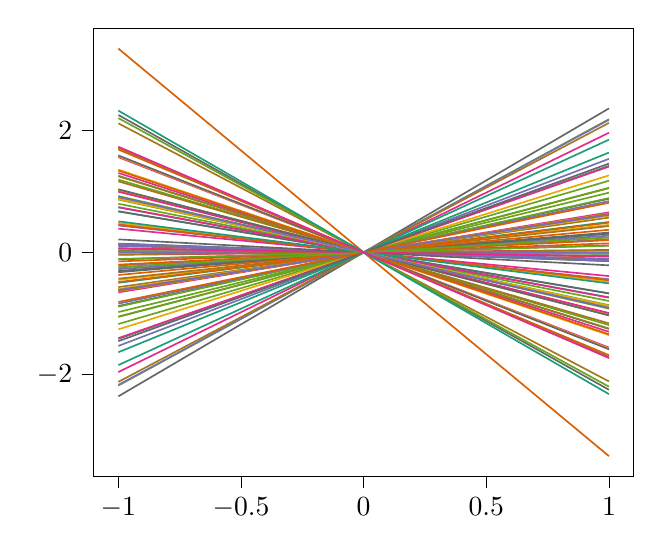
\begin{tikzpicture}

\definecolor{chocolate217952}{RGB}{217,95,2}
\definecolor{darkcyan27158119}{RGB}{27,158,119}
\definecolor{darkgoldenrod16611829}{RGB}{166,118,29}
\definecolor{darkgray176}{RGB}{176,176,176}
\definecolor{deeppink23141138}{RGB}{231,41,138}
\definecolor{dimgray102}{RGB}{102,102,102}
\definecolor{lightslategray117112179}{RGB}{117,112,179}
\definecolor{olivedrab10216630}{RGB}{102,166,30}
\definecolor{orange2301712}{RGB}{230,171,2}

\begin{axis}[
tick align=outside,
tick pos=left,
x grid style={darkgray176},
xmin=-1.1, xmax=1.1,
xtick style={color=black},
y grid style={darkgray176},
ymin=-3.66692908026053, ymax=3.66692908026053,
ytick style={color=black}
]
\addplot [semithick, darkcyan27158119]
table {%
-1 -0.497875773473803
-0.97979797979798 -0.487817677039989
-0.95959595959596 -0.477759580606175
-0.939393939393939 -0.467701484172361
-0.919191919191919 -0.457643387738546
-0.898989898989899 -0.447585291304732
-0.878787878787879 -0.437527194870918
-0.858585858585859 -0.427469098437104
-0.838383838383838 -0.41741100200329
-0.818181818181818 -0.407352905569475
-0.797979797979798 -0.397294809135661
-0.777777777777778 -0.387236712701847
-0.757575757575758 -0.377178616268033
-0.737373737373737 -0.367120519834219
-0.717171717171717 -0.357062423400404
-0.696969696969697 -0.34700432696659
-0.676767676767677 -0.336946230532776
-0.656565656565657 -0.326888134098962
-0.636363636363636 -0.316830037665148
-0.616161616161616 -0.306771941231333
-0.595959595959596 -0.296713844797519
-0.575757575757576 -0.286655748363705
-0.555555555555556 -0.276597651929891
-0.535353535353535 -0.266539555496076
-0.515151515151515 -0.256481459062262
-0.494949494949495 -0.246423362628448
-0.474747474747475 -0.236365266194634
-0.454545454545454 -0.22630716976082
-0.434343434343434 -0.216249073327005
-0.414141414141414 -0.206190976893191
-0.393939393939394 -0.196132880459377
-0.373737373737374 -0.186074784025563
-0.353535353535353 -0.176016687591749
-0.333333333333333 -0.165958591157934
-0.313131313131313 -0.15590049472412
-0.292929292929293 -0.145842398290306
-0.272727272727273 -0.135784301856492
-0.252525252525252 -0.125726205422678
-0.232323232323232 -0.115668108988863
-0.212121212121212 -0.105610012555049
-0.191919191919192 -0.0955519161212349
-0.171717171717172 -0.0854938196874207
-0.151515151515151 -0.0754357232536065
-0.131313131313131 -0.0653776268197923
-0.111111111111111 -0.0553195303859781
-0.0909090909090908 -0.0452614339521639
-0.0707070707070706 -0.0352033375183497
-0.0505050505050504 -0.0251452410845355
-0.0303030303030303 -0.0150871446507213
-0.0101010101010101 -0.00502904821690708
0.0101010101010102 0.00502904821690713
0.0303030303030305 0.0150871446507214
0.0505050505050506 0.0251452410845356
0.0707070707070707 0.0352033375183497
0.0909090909090911 0.045261433952164
0.111111111111111 0.0553195303859782
0.131313131313131 0.0653776268197924
0.151515151515152 0.0754357232536066
0.171717171717172 0.0854938196874207
0.191919191919192 0.095551916121235
0.212121212121212 0.105610012555049
0.232323232323232 0.115668108988863
0.252525252525253 0.125726205422678
0.272727272727273 0.135784301856492
0.292929292929293 0.145842398290306
0.313131313131313 0.15590049472412
0.333333333333333 0.165958591157934
0.353535353535354 0.176016687591749
0.373737373737374 0.186074784025563
0.393939393939394 0.196132880459377
0.414141414141414 0.206190976893191
0.434343434343434 0.216249073327005
0.454545454545455 0.22630716976082
0.474747474747475 0.236365266194634
0.494949494949495 0.246423362628448
0.515151515151515 0.256481459062262
0.535353535353535 0.266539555496076
0.555555555555556 0.276597651929891
0.575757575757576 0.286655748363705
0.595959595959596 0.296713844797519
0.616161616161616 0.306771941231333
0.636363636363636 0.316830037665148
0.656565656565657 0.326888134098962
0.676767676767677 0.336946230532776
0.696969696969697 0.34700432696659
0.717171717171717 0.357062423400404
0.737373737373737 0.367120519834219
0.757575757575758 0.377178616268033
0.777777777777778 0.387236712701847
0.797979797979798 0.397294809135661
0.818181818181818 0.407352905569475
0.838383838383838 0.41741100200329
0.858585858585859 0.427469098437104
0.878787878787879 0.437527194870918
0.898989898989899 0.447585291304732
0.919191919191919 0.457643387738546
0.939393939393939 0.467701484172361
0.95959595959596 0.477759580606175
0.97979797979798 0.487817677039989
1 0.497875773473803
};
\addplot [semithick, chocolate217952]
table {%
-1 -0.246317997684563
-0.97979797979798 -0.241341876519218
-0.95959595959596 -0.236365755353873
-0.939393939393939 -0.231389634188529
-0.919191919191919 -0.226413513023184
-0.898989898989899 -0.221437391857839
-0.878787878787879 -0.216461270692495
-0.858585858585859 -0.21148514952715
-0.838383838383838 -0.206509028361805
-0.818181818181818 -0.20153290719646
-0.797979797979798 -0.196556786031116
-0.777777777777778 -0.191580664865771
-0.757575757575758 -0.186604543700426
-0.737373737373737 -0.181628422535082
-0.717171717171717 -0.176652301369737
-0.696969696969697 -0.171676180204392
-0.676767676767677 -0.166700059039047
-0.656565656565657 -0.161723937873703
-0.636363636363636 -0.156747816708358
-0.616161616161616 -0.151771695543013
-0.595959595959596 -0.146795574377669
-0.575757575757576 -0.141819453212324
-0.555555555555556 -0.136843332046979
-0.535353535353535 -0.131867210881635
-0.515151515151515 -0.12689108971629
-0.494949494949495 -0.121914968550945
-0.474747474747475 -0.1169388473856
-0.454545454545454 -0.111962726220256
-0.434343434343434 -0.106986605054911
-0.414141414141414 -0.102010483889566
-0.393939393939394 -0.0970343627242217
-0.373737373737374 -0.092058241558877
-0.353535353535353 -0.0870821203935323
-0.333333333333333 -0.0821059992281876
-0.313131313131313 -0.0771298780628429
-0.292929292929293 -0.0721537568974982
-0.272727272727273 -0.0671776357321535
-0.252525252525252 -0.0622015145668088
-0.232323232323232 -0.0572253934014641
-0.212121212121212 -0.0522492722361194
-0.191919191919192 -0.0472731510707746
-0.171717171717172 -0.0422970299054299
-0.151515151515151 -0.0373209087400853
-0.131313131313131 -0.0323447875747406
-0.111111111111111 -0.0273686664093958
-0.0909090909090908 -0.0223925452440511
-0.0707070707070706 -0.0174164240787064
-0.0505050505050504 -0.0124403029133617
-0.0303030303030303 -0.00746418174801705
-0.0101010101010101 -0.00248806058267234
0.0101010101010102 0.00248806058267237
0.0303030303030305 0.0074641817480171
0.0505050505050506 0.0124403029133618
0.0707070707070707 0.0174164240787065
0.0909090909090911 0.0223925452440512
0.111111111111111 0.0273686664093959
0.131313131313131 0.0323447875747406
0.151515151515152 0.0373209087400853
0.171717171717172 0.04229702990543
0.191919191919192 0.0472731510707747
0.212121212121212 0.0522492722361194
0.232323232323232 0.0572253934014641
0.252525252525253 0.0622015145668088
0.272727272727273 0.0671776357321535
0.292929292929293 0.0721537568974982
0.313131313131313 0.0771298780628429
0.333333333333333 0.0821059992281876
0.353535353535354 0.0870821203935323
0.373737373737374 0.092058241558877
0.393939393939394 0.0970343627242217
0.414141414141414 0.102010483889566
0.434343434343434 0.106986605054911
0.454545454545455 0.111962726220256
0.474747474747475 0.116938847385601
0.494949494949495 0.121914968550945
0.515151515151515 0.12689108971629
0.535353535353535 0.131867210881635
0.555555555555556 0.136843332046979
0.575757575757576 0.141819453212324
0.595959595959596 0.146795574377669
0.616161616161616 0.151771695543013
0.636363636363636 0.156747816708358
0.656565656565657 0.161723937873703
0.676767676767677 0.166700059039048
0.696969696969697 0.171676180204392
0.717171717171717 0.176652301369737
0.737373737373737 0.181628422535082
0.757575757575758 0.186604543700426
0.777777777777778 0.191580664865771
0.797979797979798 0.196556786031116
0.818181818181818 0.20153290719646
0.838383838383838 0.206509028361805
0.858585858585859 0.21148514952715
0.878787878787879 0.216461270692495
0.898989898989899 0.221437391857839
0.919191919191919 0.226413513023184
0.939393939393939 0.231389634188529
0.95959595959596 0.236365755353873
0.97979797979798 0.241341876519218
1 0.246317997684563
};
\addplot [semithick, lightslategray117112179]
table {%
-1 -0.638559903895984
-0.97979797979798 -0.625659703817277
-0.95959595959596 -0.612759503738571
-0.939393939393939 -0.599859303659864
-0.919191919191919 -0.586959103581157
-0.898989898989899 -0.57405890350245
-0.878787878787879 -0.561158703423744
-0.858585858585859 -0.548258503345037
-0.838383838383838 -0.53535830326633
-0.818181818181818 -0.522458103187623
-0.797979797979798 -0.509557903108917
-0.777777777777778 -0.49665770303021
-0.757575757575758 -0.483757502951503
-0.737373737373737 -0.470857302872796
-0.717171717171717 -0.45795710279409
-0.696969696969697 -0.445056902715383
-0.676767676767677 -0.432156702636676
-0.656565656565657 -0.419256502557969
-0.636363636363636 -0.406356302479263
-0.616161616161616 -0.393456102400556
-0.595959595959596 -0.380555902321849
-0.575757575757576 -0.367655702243142
-0.555555555555556 -0.354755502164436
-0.535353535353535 -0.341855302085729
-0.515151515151515 -0.328955102007022
-0.494949494949495 -0.316054901928315
-0.474747474747475 -0.303154701849609
-0.454545454545454 -0.290254501770902
-0.434343434343434 -0.277354301692195
-0.414141414141414 -0.264454101613488
-0.393939393939394 -0.251553901534782
-0.373737373737374 -0.238653701456075
-0.353535353535353 -0.225753501377368
-0.333333333333333 -0.212853301298661
-0.313131313131313 -0.199953101219955
-0.292929292929293 -0.187052901141248
-0.272727272727273 -0.174152701062541
-0.252525252525252 -0.161252500983834
-0.232323232323232 -0.148352300905128
-0.212121212121212 -0.135452100826421
-0.191919191919192 -0.122551900747714
-0.171717171717172 -0.109651700669007
-0.151515151515151 -0.0967515005903006
-0.131313131313131 -0.0838513005115938
-0.111111111111111 -0.0709511004328871
-0.0909090909090908 -0.0580509003541803
-0.0707070707070706 -0.0451507002754736
-0.0505050505050504 -0.0322505001967668
-0.0303030303030303 -0.0193503001180601
-0.0101010101010101 -0.00645010003935334
0.0101010101010102 0.00645010003935342
0.0303030303030305 0.0193503001180602
0.0505050505050506 0.0322505001967669
0.0707070707070707 0.0451507002754736
0.0909090909090911 0.0580509003541805
0.111111111111111 0.0709511004328871
0.131313131313131 0.083851300511594
0.151515151515152 0.0967515005903007
0.171717171717172 0.109651700669007
0.191919191919192 0.122551900747714
0.212121212121212 0.135452100826421
0.232323232323232 0.148352300905128
0.252525252525253 0.161252500983834
0.272727272727273 0.174152701062541
0.292929292929293 0.187052901141248
0.313131313131313 0.199953101219955
0.333333333333333 0.212853301298661
0.353535353535354 0.225753501377368
0.373737373737374 0.238653701456075
0.393939393939394 0.251553901534782
0.414141414141414 0.264454101613488
0.434343434343434 0.277354301692195
0.454545454545455 0.290254501770902
0.474747474747475 0.303154701849609
0.494949494949495 0.316054901928315
0.515151515151515 0.328955102007022
0.535353535353535 0.341855302085729
0.555555555555556 0.354755502164436
0.575757575757576 0.367655702243142
0.595959595959596 0.380555902321849
0.616161616161616 0.393456102400556
0.636363636363636 0.406356302479263
0.656565656565657 0.419256502557969
0.676767676767677 0.432156702636676
0.696969696969697 0.445056902715383
0.717171717171717 0.45795710279409
0.737373737373737 0.470857302872796
0.757575757575758 0.483757502951503
0.777777777777778 0.49665770303021
0.797979797979798 0.509557903108917
0.818181818181818 0.522458103187623
0.838383838383838 0.53535830326633
0.858585858585859 0.548258503345037
0.878787878787879 0.561158703423744
0.898989898989899 0.57405890350245
0.919191919191919 0.586959103581157
0.939393939393939 0.599859303659864
0.95959595959596 0.612759503738571
0.97979797979798 0.625659703817277
1 0.638559903895984
};
\addplot [semithick, deeppink23141138]
table {%
-1 1.55765215131277
-0.97979797979798 1.52618443108423
-0.95959595959596 1.49471671085569
-0.939393939393939 1.46324899062714
-0.919191919191919 1.4317812703986
-0.898989898989899 1.40031355017006
-0.878787878787879 1.36884582994152
-0.858585858585859 1.33737810971298
-0.838383838383838 1.30591038948444
-0.818181818181818 1.2744426692559
-0.797979797979798 1.24297494902736
-0.777777777777778 1.21150722879882
-0.757575757575758 1.18003950857028
-0.737373737373737 1.14857178834174
-0.717171717171717 1.1171040681132
-0.696969696969697 1.08563634788466
-0.676767676767677 1.05416862765611
-0.656565656565657 1.02270090742757
-0.636363636363636 0.991233187199034
-0.616161616161616 0.959765466970493
-0.595959595959596 0.928297746741952
-0.575757575757576 0.896830026513411
-0.555555555555556 0.865362306284871
-0.535353535353535 0.83389458605633
-0.515151515151515 0.802426865827789
-0.494949494949495 0.770959145599248
-0.474747474747475 0.739491425370707
-0.454545454545454 0.708023705142167
-0.434343434343434 0.676555984913626
-0.414141414141414 0.645088264685085
-0.393939393939394 0.613620544456545
-0.373737373737374 0.582152824228004
-0.353535353535353 0.550685103999463
-0.333333333333333 0.519217383770922
-0.313131313131313 0.487749663542381
-0.292929292929293 0.456281943313841
-0.272727272727273 0.4248142230853
-0.252525252525252 0.393346502856759
-0.232323232323232 0.361878782628218
-0.212121212121212 0.330411062399678
-0.191919191919192 0.298943342171137
-0.171717171717172 0.267475621942596
-0.151515151515151 0.236007901714056
-0.131313131313131 0.204540181485515
-0.111111111111111 0.173072461256974
-0.0909090909090908 0.141604741028433
-0.0707070707070706 0.110137020799892
-0.0505050505050504 0.0786693005713517
-0.0303030303030303 0.0472015803428111
-0.0101010101010101 0.0157338601142703
0.0101010101010102 -0.0157338601142705
0.0303030303030305 -0.0472015803428114
0.0505050505050506 -0.078669300571352
0.0707070707070707 -0.110137020799893
0.0909090909090911 -0.141604741028434
0.111111111111111 -0.173072461256974
0.131313131313131 -0.204540181485515
0.151515151515152 -0.236007901714056
0.171717171717172 -0.267475621942596
0.191919191919192 -0.298943342171137
0.212121212121212 -0.330411062399678
0.232323232323232 -0.361878782628219
0.252525252525253 -0.393346502856759
0.272727272727273 -0.4248142230853
0.292929292929293 -0.456281943313841
0.313131313131313 -0.487749663542382
0.333333333333333 -0.519217383770923
0.353535353535354 -0.550685103999463
0.373737373737374 -0.582152824228004
0.393939393939394 -0.613620544456545
0.414141414141414 -0.645088264685086
0.434343434343434 -0.676555984913626
0.454545454545455 -0.708023705142167
0.474747474747475 -0.739491425370708
0.494949494949495 -0.770959145599248
0.515151515151515 -0.802426865827789
0.535353535353535 -0.83389458605633
0.555555555555556 -0.865362306284871
0.575757575757576 -0.896830026513412
0.595959595959596 -0.928297746741952
0.616161616161616 -0.959765466970493
0.636363636363636 -0.991233187199034
0.656565656565657 -1.02270090742757
0.676767676767677 -1.05416862765612
0.696969696969697 -1.08563634788466
0.717171717171717 -1.1171040681132
0.737373737373737 -1.14857178834174
0.757575757575758 -1.18003950857028
0.777777777777778 -1.21150722879882
0.797979797979798 -1.24297494902736
0.818181818181818 -1.2744426692559
0.838383838383838 -1.30591038948444
0.858585858585859 -1.33737810971298
0.878787878787879 -1.36884582994152
0.898989898989899 -1.40031355017006
0.919191919191919 -1.4317812703986
0.939393939393939 -1.46324899062714
0.95959595959596 -1.49471671085569
0.97979797979798 -1.52618443108423
1 -1.55765215131277
};
\addplot [semithick, olivedrab10216630]
table {%
-1 -2.17852231889229
-0.97979797979798 -2.13451176699548
-0.95959595959596 -2.09050121509866
-0.939393939393939 -2.04649066320185
-0.919191919191919 -2.00248011130503
-0.898989898989899 -1.95846955940822
-0.878787878787879 -1.91445900751141
-0.858585858585859 -1.87044845561459
-0.838383838383838 -1.82643790371778
-0.818181818181818 -1.78242735182096
-0.797979797979798 -1.73841679992415
-0.777777777777778 -1.69440624802734
-0.757575757575758 -1.65039569613052
-0.737373737373737 -1.60638514423371
-0.717171717171717 -1.56237459233689
-0.696969696969697 -1.51836404044008
-0.676767676767677 -1.47435348854327
-0.656565656565657 -1.43034293664645
-0.636363636363636 -1.38633238474964
-0.616161616161616 -1.34232183285283
-0.595959595959596 -1.29831128095601
-0.575757575757576 -1.2543007290592
-0.555555555555556 -1.21029017716238
-0.535353535353535 -1.16627962526557
-0.515151515151515 -1.12226907336876
-0.494949494949495 -1.07825852147194
-0.474747474747475 -1.03424796957513
-0.454545454545454 -0.990237417678314
-0.434343434343434 -0.9462268657815
-0.414141414141414 -0.902216313884686
-0.393939393939394 -0.858205761987872
-0.373737373737374 -0.814195210091058
-0.353535353535353 -0.770184658194244
-0.333333333333333 -0.72617410629743
-0.313131313131313 -0.682163554400616
-0.292929292929293 -0.638153002503802
-0.272727272727273 -0.594142450606988
-0.252525252525252 -0.550131898710174
-0.232323232323232 -0.50612134681336
-0.212121212121212 -0.462110794916546
-0.191919191919192 -0.418100243019732
-0.171717171717172 -0.374089691122918
-0.151515151515151 -0.330079139226104
-0.131313131313131 -0.286068587329291
-0.111111111111111 -0.242058035432477
-0.0909090909090908 -0.198047483535663
-0.0707070707070706 -0.154036931638849
-0.0505050505050504 -0.110026379742035
-0.0303030303030303 -0.0660158278452209
-0.0101010101010101 -0.0220052759484069
0.0101010101010102 0.0220052759484071
0.0303030303030305 0.0660158278452213
0.0505050505050506 0.110026379742035
0.0707070707070707 0.154036931638849
0.0909090909090911 0.198047483535663
0.111111111111111 0.242058035432477
0.131313131313131 0.286068587329291
0.151515151515152 0.330079139226105
0.171717171717172 0.374089691122918
0.191919191919192 0.418100243019733
0.212121212121212 0.462110794916546
0.232323232323232 0.506121346813361
0.252525252525253 0.550131898710174
0.272727272727273 0.594142450606989
0.292929292929293 0.638153002503802
0.313131313131313 0.682163554400616
0.333333333333333 0.72617410629743
0.353535353535354 0.770184658194244
0.373737373737374 0.814195210091058
0.393939393939394 0.858205761987872
0.414141414141414 0.902216313884686
0.434343434343434 0.9462268657815
0.454545454545455 0.990237417678314
0.474747474747475 1.03424796957513
0.494949494949495 1.07825852147194
0.515151515151515 1.12226907336876
0.535353535353535 1.16627962526557
0.555555555555556 1.21029017716238
0.575757575757576 1.2543007290592
0.595959595959596 1.29831128095601
0.616161616161616 1.34232183285283
0.636363636363636 1.38633238474964
0.656565656565657 1.43034293664645
0.676767676767677 1.47435348854327
0.696969696969697 1.51836404044008
0.717171717171717 1.5623745923369
0.737373737373737 1.60638514423371
0.757575757575758 1.65039569613052
0.777777777777778 1.69440624802734
0.797979797979798 1.73841679992415
0.818181818181818 1.78242735182096
0.838383838383838 1.82643790371778
0.858585858585859 1.87044845561459
0.878787878787879 1.91445900751141
0.898989898989899 1.95846955940822
0.919191919191919 2.00248011130503
0.939393939393939 2.04649066320185
0.95959595959596 2.09050121509866
0.97979797979798 2.13451176699548
1 2.17852231889229
};
\addplot [semithick, orange2301712]
table {%
-1 0.922435593374344
-0.97979797979798 0.903800530881933
-0.95959595959596 0.885165468389522
-0.939393939393939 0.866530405897111
-0.919191919191919 0.847895343404701
-0.898989898989899 0.829260280912289
-0.878787878787879 0.810625218419878
-0.858585858585859 0.791990155927467
-0.838383838383838 0.773355093435056
-0.818181818181818 0.754720030942645
-0.797979797979798 0.736084968450235
-0.777777777777778 0.717449905957823
-0.757575757575758 0.698814843465412
-0.737373737373737 0.680179780973001
-0.717171717171717 0.66154471848059
-0.696969696969697 0.64290965598818
-0.676767676767677 0.624274593495768
-0.656565656565657 0.605639531003357
-0.636363636363636 0.587004468510946
-0.616161616161616 0.568369406018535
-0.595959595959596 0.549734343526124
-0.575757575757576 0.531099281033713
-0.555555555555556 0.512464218541303
-0.535353535353535 0.493829156048891
-0.515151515151515 0.47519409355648
-0.494949494949495 0.456559031064069
-0.474747474747475 0.437923968571658
-0.454545454545454 0.419288906079247
-0.434343434343434 0.400653843586836
-0.414141414141414 0.382018781094425
-0.393939393939394 0.363383718602014
-0.373737373737374 0.344748656109603
-0.353535353535353 0.326113593617192
-0.333333333333333 0.307478531124781
-0.313131313131313 0.28884346863237
-0.292929292929293 0.270208406139959
-0.272727272727273 0.251573343647548
-0.252525252525252 0.232938281155137
-0.232323232323232 0.214303218662726
-0.212121212121212 0.195668156170315
-0.191919191919192 0.177033093677904
-0.171717171717172 0.158398031185493
-0.151515151515151 0.139762968693082
-0.131313131313131 0.121127906200671
-0.111111111111111 0.10249284370826
-0.0909090909090908 0.0838577812158494
-0.0707070707070706 0.0652227187234384
-0.0505050505050504 0.0465876562310274
-0.0303030303030303 0.0279525937386165
-0.0101010101010101 0.00931753124620546
0.0101010101010102 -0.00931753124620556
0.0303030303030305 -0.0279525937386167
0.0505050505050506 -0.0465876562310276
0.0707070707070707 -0.0652227187234385
0.0909090909090911 -0.0838577812158496
0.111111111111111 -0.102492843708261
0.131313131313131 -0.121127906200672
0.151515151515152 -0.139762968693083
0.171717171717172 -0.158398031185493
0.191919191919192 -0.177033093677905
0.212121212121212 -0.195668156170316
0.232323232323232 -0.214303218662727
0.252525252525253 -0.232938281155138
0.272727272727273 -0.251573343647549
0.292929292929293 -0.27020840613996
0.313131313131313 -0.28884346863237
0.333333333333333 -0.307478531124782
0.353535353535354 -0.326113593617193
0.373737373737374 -0.344748656109604
0.393939393939394 -0.363383718602015
0.414141414141414 -0.382018781094426
0.434343434343434 -0.400653843586837
0.454545454545455 -0.419288906079248
0.474747474747475 -0.437923968571659
0.494949494949495 -0.45655903106407
0.515151515151515 -0.475194093556481
0.535353535353535 -0.493829156048892
0.555555555555556 -0.512464218541303
0.575757575757576 -0.531099281033714
0.595959595959596 -0.549734343526124
0.616161616161616 -0.568369406018536
0.636363636363636 -0.587004468510947
0.656565656565657 -0.605639531003358
0.676767676767677 -0.624274593495769
0.696969696969697 -0.64290965598818
0.717171717171717 -0.661544718480591
0.737373737373737 -0.680179780973002
0.757575757575758 -0.698814843465413
0.777777777777778 -0.717449905957824
0.797979797979798 -0.736084968450235
0.818181818181818 -0.754720030942646
0.838383838383838 -0.773355093435056
0.858585858585859 -0.791990155927468
0.878787878787879 -0.810625218419879
0.898989898989899 -0.82926028091229
0.919191919191919 -0.847895343404701
0.939393939393939 -0.866530405897111
0.95959595959596 -0.885165468389523
0.97979797979798 -0.903800530881934
1 -0.922435593374344
};
\addplot [semithick, darkgoldenrod16611829]
table {%
-1 -0.568431589935611
-0.97979797979798 -0.556948123472266
-0.95959595959596 -0.54546465700892
-0.939393939393939 -0.533981190545574
-0.919191919191919 -0.522497724082229
-0.898989898989899 -0.511014257618883
-0.878787878787879 -0.499530791155537
-0.858585858585859 -0.488047324692192
-0.838383838383838 -0.476563858228846
-0.818181818181818 -0.4650803917655
-0.797979797979798 -0.453596925302155
-0.777777777777778 -0.442113458838809
-0.757575757575758 -0.430629992375463
-0.737373737373737 -0.419146525912118
-0.717171717171717 -0.407663059448772
-0.696969696969697 -0.396179592985426
-0.676767676767677 -0.38469612652208
-0.656565656565657 -0.373212660058735
-0.636363636363636 -0.361729193595389
-0.616161616161616 -0.350245727132043
-0.595959595959596 -0.338762260668698
-0.575757575757576 -0.327278794205352
-0.555555555555556 -0.315795327742006
-0.535353535353535 -0.304311861278661
-0.515151515151515 -0.292828394815315
-0.494949494949495 -0.281344928351969
-0.474747474747475 -0.269861461888624
-0.454545454545454 -0.258377995425278
-0.434343434343434 -0.246894528961932
-0.414141414141414 -0.235411062498587
-0.393939393939394 -0.223927596035241
-0.373737373737374 -0.212444129571895
-0.353535353535353 -0.200960663108549
-0.333333333333333 -0.189477196645204
-0.313131313131313 -0.177993730181858
-0.292929292929293 -0.166510263718512
-0.272727272727273 -0.155026797255167
-0.252525252525252 -0.143543330791821
-0.232323232323232 -0.132059864328475
-0.212121212121212 -0.12057639786513
-0.191919191919192 -0.109092931401784
-0.171717171717172 -0.0976094649384383
-0.151515151515151 -0.0861259984750926
-0.131313131313131 -0.0746425320117469
-0.111111111111111 -0.0631590655484012
-0.0909090909090908 -0.0516755990850555
-0.0707070707070706 -0.0401921326217098
-0.0505050505050504 -0.0287086661583641
-0.0303030303030303 -0.0172251996950185
-0.0101010101010101 -0.00574173323167282
0.0101010101010102 0.00574173323167288
0.0303030303030305 0.0172251996950186
0.0505050505050506 0.0287086661583643
0.0707070707070707 0.0401921326217099
0.0909090909090911 0.0516755990850557
0.111111111111111 0.0631590655484013
0.131313131313131 0.0746425320117471
0.151515151515152 0.0861259984750927
0.171717171717172 0.0976094649384383
0.191919191919192 0.109092931401784
0.212121212121212 0.12057639786513
0.232323232323232 0.132059864328475
0.252525252525253 0.143543330791821
0.272727272727273 0.155026797255167
0.292929292929293 0.166510263718513
0.313131313131313 0.177993730181858
0.333333333333333 0.189477196645204
0.353535353535354 0.20096066310855
0.373737373737374 0.212444129571895
0.393939393939394 0.223927596035241
0.414141414141414 0.235411062498587
0.434343434343434 0.246894528961932
0.454545454545455 0.258377995425278
0.474747474747475 0.269861461888624
0.494949494949495 0.281344928351969
0.515151515151515 0.292828394815315
0.535353535353535 0.304311861278661
0.555555555555556 0.315795327742006
0.575757575757576 0.327278794205352
0.595959595959596 0.338762260668698
0.616161616161616 0.350245727132044
0.636363636363636 0.361729193595389
0.656565656565657 0.373212660058735
0.676767676767677 0.384696126522081
0.696969696969697 0.396179592985426
0.717171717171717 0.407663059448772
0.737373737373737 0.419146525912118
0.757575757575758 0.430629992375463
0.777777777777778 0.442113458838809
0.797979797979798 0.453596925302155
0.818181818181818 0.4650803917655
0.838383838383838 0.476563858228846
0.858585858585859 0.488047324692192
0.878787878787879 0.499530791155537
0.898989898989899 0.511014257618883
0.919191919191919 0.522497724082229
0.939393939393939 0.533981190545574
0.95959595959596 0.54546465700892
0.97979797979798 0.556948123472266
1 0.568431589935611
};
\addplot [semithick, dimgray102]
table {%
-1 -0.877526016306959
-0.97979797979798 -0.859798217997727
-0.95959595959596 -0.842070419688496
-0.939393939393939 -0.824342621379265
-0.919191919191919 -0.806614823070033
-0.898989898989899 -0.788887024760802
-0.878787878787879 -0.77115922645157
-0.858585858585859 -0.753431428142339
-0.838383838383838 -0.735703629833107
-0.818181818181818 -0.717975831523876
-0.797979797979798 -0.700248033214644
-0.777777777777778 -0.682520234905413
-0.757575757575758 -0.664792436596181
-0.737373737373737 -0.64706463828695
-0.717171717171717 -0.629336839977718
-0.696969696969697 -0.611609041668487
-0.676767676767677 -0.593881243359255
-0.656565656565657 -0.576153445050024
-0.636363636363636 -0.558425646740792
-0.616161616161616 -0.540697848431561
-0.595959595959596 -0.522970050122329
-0.575757575757576 -0.505242251813098
-0.555555555555556 -0.487514453503866
-0.535353535353535 -0.469786655194635
-0.515151515151515 -0.452058856885403
-0.494949494949495 -0.434331058576172
-0.474747474747475 -0.41660326026694
-0.454545454545454 -0.398875461957709
-0.434343434343434 -0.381147663648477
-0.414141414141414 -0.363419865339246
-0.393939393939394 -0.345692067030014
-0.373737373737374 -0.327964268720783
-0.353535353535353 -0.310236470411551
-0.333333333333333 -0.29250867210232
-0.313131313131313 -0.274780873793088
-0.292929292929293 -0.257053075483857
-0.272727272727273 -0.239325277174625
-0.252525252525252 -0.221597478865394
-0.232323232323232 -0.203869680556162
-0.212121212121212 -0.186141882246931
-0.191919191919192 -0.168414083937699
-0.171717171717172 -0.150686285628468
-0.151515151515151 -0.132958487319236
-0.131313131313131 -0.115230689010005
-0.111111111111111 -0.0975028907007732
-0.0909090909090908 -0.0797750923915417
-0.0707070707070706 -0.0620472940823101
-0.0505050505050504 -0.0443194957730786
-0.0303030303030303 -0.0265916974638472
-0.0101010101010101 -0.00886389915461571
0.0101010101010102 0.0088638991546158
0.0303030303030305 0.0265916974638474
0.0505050505050506 0.0443194957730788
0.0707070707070707 0.0620472940823102
0.0909090909090911 0.0797750923915419
0.111111111111111 0.0975028907007733
0.131313131313131 0.115230689010005
0.151515151515152 0.132958487319236
0.171717171717172 0.150686285628468
0.191919191919192 0.168414083937699
0.212121212121212 0.186141882246931
0.232323232323232 0.203869680556162
0.252525252525253 0.221597478865394
0.272727272727273 0.239325277174625
0.292929292929293 0.257053075483857
0.313131313131313 0.274780873793088
0.333333333333333 0.29250867210232
0.353535353535354 0.310236470411551
0.373737373737374 0.327964268720783
0.393939393939394 0.345692067030014
0.414141414141414 0.363419865339246
0.434343434343434 0.381147663648477
0.454545454545455 0.398875461957709
0.474747474747475 0.41660326026694
0.494949494949495 0.434331058576172
0.515151515151515 0.452058856885403
0.535353535353535 0.469786655194635
0.555555555555556 0.487514453503866
0.575757575757576 0.505242251813098
0.595959595959596 0.522970050122329
0.616161616161616 0.540697848431561
0.636363636363636 0.558425646740792
0.656565656565657 0.576153445050024
0.676767676767677 0.593881243359255
0.696969696969697 0.611609041668487
0.717171717171717 0.629336839977718
0.737373737373737 0.64706463828695
0.757575757575758 0.664792436596181
0.777777777777778 0.682520234905413
0.797979797979798 0.700248033214644
0.818181818181818 0.717975831523876
0.838383838383838 0.735703629833107
0.858585858585859 0.753431428142339
0.878787878787879 0.77115922645157
0.898989898989899 0.788887024760802
0.919191919191919 0.806614823070033
0.939393939393939 0.824342621379265
0.95959595959596 0.842070419688496
0.97979797979798 0.859798217997728
1 0.877526016306959
};
\addplot [semithick, darkcyan27158119]
table {%
-1 0.140461335540084
-0.97979797979798 0.1376237328019
-0.95959595959596 0.134786130063717
-0.939393939393939 0.131948527325533
-0.919191919191919 0.12911092458735
-0.898989898989899 0.126273321849166
-0.878787878787879 0.123435719110983
-0.858585858585859 0.120598116372799
-0.838383838383838 0.117760513634616
-0.818181818181818 0.114922910896432
-0.797979797979798 0.112085308158249
-0.777777777777778 0.109247705420065
-0.757575757575758 0.106410102681882
-0.737373737373737 0.103572499943698
-0.717171717171717 0.100734897205515
-0.696969696969697 0.0978972944673312
-0.676767676767677 0.0950596917291477
-0.656565656565657 0.0922220889909642
-0.636363636363636 0.0893844862527807
-0.616161616161616 0.0865468835145972
-0.595959595959596 0.0837092807764136
-0.575757575757576 0.0808716780382301
-0.555555555555556 0.0780340753000466
-0.535353535353535 0.0751964725618631
-0.515151515151515 0.0723588698236796
-0.494949494949495 0.0695212670854961
-0.474747474747475 0.0666836643473126
-0.454545454545454 0.063846061609129
-0.434343434343434 0.0610084588709455
-0.414141414141414 0.058170856132762
-0.393939393939394 0.0553332533945785
-0.373737373737374 0.052495650656395
-0.353535353535353 0.0496580479182115
-0.333333333333333 0.046820445180028
-0.313131313131313 0.0439828424418444
-0.292929292929293 0.0411452397036609
-0.272727272727273 0.0383076369654774
-0.252525252525252 0.0354700342272939
-0.232323232323232 0.0326324314891104
-0.212121212121212 0.0297948287509269
-0.191919191919192 0.0269572260127434
-0.171717171717172 0.0241196232745598
-0.151515151515151 0.0212820205363763
-0.131313131313131 0.0184444177981928
-0.111111111111111 0.0156068150600093
-0.0909090909090908 0.0127692123218258
-0.0707070707070706 0.00993160958364228
-0.0505050505050504 0.00709400684545877
-0.0303030303030303 0.00425640410727527
-0.0101010101010101 0.00141880136909175
0.0101010101010102 -0.00141880136909177
0.0303030303030305 -0.0042564041072753
0.0505050505050506 -0.0070940068454588
0.0707070707070707 -0.0099316095836423
0.0909090909090911 -0.0127692123218258
0.111111111111111 -0.0156068150600093
0.131313131313131 -0.0184444177981929
0.151515151515152 -0.0212820205363764
0.171717171717172 -0.0241196232745599
0.191919191919192 -0.0269572260127434
0.212121212121212 -0.0297948287509269
0.232323232323232 -0.0326324314891104
0.252525252525253 -0.0354700342272939
0.272727272727273 -0.0383076369654775
0.292929292929293 -0.041145239703661
0.313131313131313 -0.0439828424418445
0.333333333333333 -0.046820445180028
0.353535353535354 -0.0496580479182115
0.373737373737374 -0.052495650656395
0.393939393939394 -0.0553332533945785
0.414141414141414 -0.0581708561327621
0.434343434343434 -0.0610084588709456
0.454545454545455 -0.0638460616091291
0.474747474747475 -0.0666836643473126
0.494949494949495 -0.0695212670854961
0.515151515151515 -0.0723588698236796
0.535353535353535 -0.0751964725618631
0.555555555555556 -0.0780340753000466
0.575757575757576 -0.0808716780382302
0.595959595959596 -0.0837092807764137
0.616161616161616 -0.0865468835145972
0.636363636363636 -0.0893844862527807
0.656565656565657 -0.0922220889909642
0.676767676767677 -0.0950596917291477
0.696969696969697 -0.0978972944673312
0.717171717171717 -0.100734897205515
0.737373737373737 -0.103572499943698
0.757575757575758 -0.106410102681882
0.777777777777778 -0.109247705420065
0.797979797979798 -0.112085308158249
0.818181818181818 -0.114922910896432
0.838383838383838 -0.117760513634616
0.858585858585859 -0.120598116372799
0.878787878787879 -0.123435719110983
0.898989898989899 -0.126273321849166
0.919191919191919 -0.12911092458735
0.939393939393939 -0.131948527325533
0.95959595959596 -0.134786130063717
0.97979797979798 -0.1376237328019
1 -0.140461335540084
};
\addplot [semithick, chocolate217952]
table {%
-1 -0.609679403860935
-0.97979797979798 -0.597362648227381
-0.95959595959596 -0.585045892593827
-0.939393939393939 -0.572729136960273
-0.919191919191919 -0.560412381326718
-0.898989898989899 -0.548095625693164
-0.878787878787879 -0.53577887005961
-0.858585858585859 -0.523462114426056
-0.838383838383838 -0.511145358792501
-0.818181818181818 -0.498828603158947
-0.797979797979798 -0.486511847525393
-0.777777777777778 -0.474195091891839
-0.757575757575758 -0.461878336258284
-0.737373737373737 -0.44956158062473
-0.717171717171717 -0.437244824991176
-0.696969696969697 -0.424928069357622
-0.676767676767677 -0.412611313724067
-0.656565656565657 -0.400294558090513
-0.636363636363636 -0.387977802456959
-0.616161616161616 -0.375661046823405
-0.595959595959596 -0.36334429118985
-0.575757575757576 -0.351027535556296
-0.555555555555556 -0.338710779922742
-0.535353535353535 -0.326394024289188
-0.515151515151515 -0.314077268655633
-0.494949494949495 -0.301760513022079
-0.474747474747475 -0.289443757388525
-0.454545454545454 -0.277127001754971
-0.434343434343434 -0.264810246121416
-0.414141414141414 -0.252493490487862
-0.393939393939394 -0.240176734854308
-0.373737373737374 -0.227859979220754
-0.353535353535353 -0.215543223587199
-0.333333333333333 -0.203226467953645
-0.313131313131313 -0.190909712320091
-0.292929292929293 -0.178592956686537
-0.272727272727273 -0.166276201052982
-0.252525252525252 -0.153959445419428
-0.232323232323232 -0.141642689785874
-0.212121212121212 -0.12932593415232
-0.191919191919192 -0.117009178518765
-0.171717171717172 -0.104692422885211
-0.151515151515151 -0.0923756672516569
-0.131313131313131 -0.0800589116181026
-0.111111111111111 -0.0677421559845483
-0.0909090909090908 -0.0554254003509941
-0.0707070707070706 -0.0431086447174398
-0.0505050505050504 -0.0307918890838856
-0.0303030303030303 -0.0184751334503314
-0.0101010101010101 -0.0061583778167771
0.0101010101010102 0.00615837781677717
0.0303030303030305 0.0184751334503315
0.0505050505050506 0.0307918890838857
0.0707070707070707 0.0431086447174399
0.0909090909090911 0.0554254003509942
0.111111111111111 0.0677421559845484
0.131313131313131 0.0800589116181027
0.151515151515152 0.0923756672516569
0.171717171717172 0.104692422885211
0.191919191919192 0.117009178518765
0.212121212121212 0.12932593415232
0.232323232323232 0.141642689785874
0.252525252525253 0.153959445419428
0.272727272727273 0.166276201052983
0.292929292929293 0.178592956686537
0.313131313131313 0.190909712320091
0.333333333333333 0.203226467953645
0.353535353535354 0.215543223587199
0.373737373737374 0.227859979220754
0.393939393939394 0.240176734854308
0.414141414141414 0.252493490487862
0.434343434343434 0.264810246121416
0.454545454545455 0.277127001754971
0.474747474747475 0.289443757388525
0.494949494949495 0.301760513022079
0.515151515151515 0.314077268655634
0.535353535353535 0.326394024289188
0.555555555555556 0.338710779922742
0.575757575757576 0.351027535556296
0.595959595959596 0.36334429118985
0.616161616161616 0.375661046823405
0.636363636363636 0.387977802456959
0.656565656565657 0.400294558090513
0.676767676767677 0.412611313724068
0.696969696969697 0.424928069357622
0.717171717171717 0.437244824991176
0.737373737373737 0.44956158062473
0.757575757575758 0.461878336258285
0.777777777777778 0.474195091891839
0.797979797979798 0.486511847525393
0.818181818181818 0.498828603158947
0.838383838383838 0.511145358792501
0.858585858585859 0.523462114426056
0.878787878787879 0.53577887005961
0.898989898989899 0.548095625693164
0.919191919191919 0.560412381326719
0.939393939393939 0.572729136960273
0.95959595959596 0.585045892593827
0.97979797979798 0.597362648227381
1 0.609679403860935
};
\addplot [semithick, lightslategray117112179]
table {%
-1 0.439996962010409
-0.97979797979798 0.431108134495047
-0.95959595959596 0.422219306979685
-0.939393939393939 0.413330479464323
-0.919191919191919 0.404441651948962
-0.898989898989899 0.3955528244336
-0.878787878787879 0.386663996918238
-0.858585858585859 0.377775169402876
-0.838383838383838 0.368886341887514
-0.818181818181818 0.359997514372153
-0.797979797979798 0.351108686856791
-0.777777777777778 0.342219859341429
-0.757575757575758 0.333331031826067
-0.737373737373737 0.324442204310705
-0.717171717171717 0.315553376795344
-0.696969696969697 0.306664549279982
-0.676767676767677 0.29777572176462
-0.656565656565657 0.288886894249258
-0.636363636363636 0.279998066733896
-0.616161616161616 0.271109239218535
-0.595959595959596 0.262220411703173
-0.575757575757576 0.253331584187811
-0.555555555555556 0.244442756672449
-0.535353535353535 0.235553929157087
-0.515151515151515 0.226665101641726
-0.494949494949495 0.217776274126364
-0.474747474747475 0.208887446611002
-0.454545454545454 0.19999861909564
-0.434343434343434 0.191109791580279
-0.414141414141414 0.182220964064917
-0.393939393939394 0.173332136549555
-0.373737373737374 0.164443309034193
-0.353535353535353 0.155554481518831
-0.333333333333333 0.14666565400347
-0.313131313131313 0.137776826488108
-0.292929292929293 0.128887998972746
-0.272727272727273 0.119999171457384
-0.252525252525252 0.111110343942022
-0.232323232323232 0.102221516426661
-0.212121212121212 0.0933326889112988
-0.191919191919192 0.084443861395937
-0.171717171717172 0.0755550338805752
-0.151515151515151 0.0666662063652134
-0.131313131313131 0.0577773788498516
-0.111111111111111 0.0488885513344898
-0.0909090909090908 0.039999723819128
-0.0707070707070706 0.0311108963037662
-0.0505050505050504 0.0222220687884044
-0.0303030303030303 0.0133332412730427
-0.0101010101010101 0.00444441375768088
0.0101010101010102 -0.00444441375768093
0.0303030303030305 -0.0133332412730428
0.0505050505050506 -0.0222220687884045
0.0707070707070707 -0.0311108963037663
0.0909090909090911 -0.0399997238191281
0.111111111111111 -0.0488885513344899
0.131313131313131 -0.0577773788498517
0.151515151515152 -0.0666662063652135
0.171717171717172 -0.0755550338805752
0.191919191919192 -0.0844438613959371
0.212121212121212 -0.0933326889112989
0.232323232323232 -0.102221516426661
0.252525252525253 -0.111110343942022
0.272727272727273 -0.119999171457384
0.292929292929293 -0.128887998972746
0.313131313131313 -0.137776826488108
0.333333333333333 -0.14666565400347
0.353535353535354 -0.155554481518831
0.373737373737374 -0.164443309034193
0.393939393939394 -0.173332136549555
0.414141414141414 -0.182220964064917
0.434343434343434 -0.191109791580279
0.454545454545455 -0.19999861909564
0.474747474747475 -0.208887446611002
0.494949494949495 -0.217776274126364
0.515151515151515 -0.226665101641726
0.535353535353535 -0.235553929157088
0.555555555555556 -0.244442756672449
0.575757575757576 -0.253331584187811
0.595959595959596 -0.262220411703173
0.616161616161616 -0.271109239218535
0.636363636363636 -0.279998066733897
0.656565656565657 -0.288886894249258
0.676767676767677 -0.29777572176462
0.696969696969697 -0.306664549279982
0.717171717171717 -0.315553376795344
0.737373737373737 -0.324442204310705
0.757575757575758 -0.333331031826067
0.777777777777778 -0.342219859341429
0.797979797979798 -0.351108686856791
0.818181818181818 -0.359997514372153
0.838383838383838 -0.368886341887514
0.858585858585859 -0.377775169402876
0.878787878787879 -0.386663996918238
0.898989898989899 -0.3955528244336
0.919191919191919 -0.404441651948962
0.939393939393939 -0.413330479464323
0.95959595959596 -0.422219306979685
0.97979797979798 -0.431108134495047
1 -0.439996962010409
};
\addplot [semithick, deeppink23141138]
table {%
-1 -0.654454947826896
-0.97979797979798 -0.641233635749585
-0.95959595959596 -0.628012323672274
-0.939393939393939 -0.614791011594963
-0.919191919191919 -0.601569699517652
-0.898989898989899 -0.588348387440341
-0.878787878787879 -0.57512707536303
-0.858585858585859 -0.561905763285719
-0.838383838383838 -0.548684451208408
-0.818181818181818 -0.535463139131097
-0.797979797979798 -0.522241827053786
-0.777777777777778 -0.509020514976475
-0.757575757575758 -0.495799202899164
-0.737373737373737 -0.482577890821853
-0.717171717171717 -0.469356578744542
-0.696969696969697 -0.456135266667231
-0.676767676767677 -0.44291395458992
-0.656565656565657 -0.429692642512609
-0.636363636363636 -0.416471330435298
-0.616161616161616 -0.403250018357987
-0.595959595959596 -0.390028706280676
-0.575757575757576 -0.376807394203365
-0.555555555555556 -0.363586082126054
-0.535353535353535 -0.350364770048742
-0.515151515151515 -0.337143457971431
-0.494949494949495 -0.32392214589412
-0.474747474747475 -0.310700833816809
-0.454545454545454 -0.297479521739498
-0.434343434343434 -0.284258209662187
-0.414141414141414 -0.271036897584876
-0.393939393939394 -0.257815585507565
-0.373737373737374 -0.244594273430254
-0.353535353535353 -0.231372961352943
-0.333333333333333 -0.218151649275632
-0.313131313131313 -0.204930337198321
-0.292929292929293 -0.19170902512101
-0.272727272727273 -0.178487713043699
-0.252525252525252 -0.165266400966388
-0.232323232323232 -0.152045088889077
-0.212121212121212 -0.138823776811766
-0.191919191919192 -0.125602464734455
-0.171717171717172 -0.112381152657144
-0.151515151515151 -0.0991598405798328
-0.131313131313131 -0.0859385285025217
-0.111111111111111 -0.0727172164252107
-0.0909090909090908 -0.0594959043478996
-0.0707070707070706 -0.0462745922705886
-0.0505050505050504 -0.0330532801932775
-0.0303030303030303 -0.0198319681159665
-0.0101010101010101 -0.00661065603865549
0.0101010101010102 0.00661065603865556
0.0303030303030305 0.0198319681159667
0.0505050505050506 0.0330532801932777
0.0707070707070707 0.0462745922705886
0.0909090909090911 0.0594959043478998
0.111111111111111 0.0727172164252107
0.131313131313131 0.0859385285025219
0.151515151515152 0.0991598405798328
0.171717171717172 0.112381152657144
0.191919191919192 0.125602464734455
0.212121212121212 0.138823776811766
0.232323232323232 0.152045088889077
0.252525252525253 0.165266400966388
0.272727272727273 0.178487713043699
0.292929292929293 0.19170902512101
0.313131313131313 0.204930337198321
0.333333333333333 0.218151649275632
0.353535353535354 0.231372961352943
0.373737373737374 0.244594273430254
0.393939393939394 0.257815585507565
0.414141414141414 0.271036897584876
0.434343434343434 0.284258209662187
0.454545454545455 0.297479521739498
0.474747474747475 0.31070083381681
0.494949494949495 0.32392214589412
0.515151515151515 0.337143457971432
0.535353535353535 0.350364770048743
0.555555555555556 0.363586082126054
0.575757575757576 0.376807394203365
0.595959595959596 0.390028706280676
0.616161616161616 0.403250018357987
0.636363636363636 0.416471330435298
0.656565656565657 0.429692642512609
0.676767676767677 0.44291395458992
0.696969696969697 0.456135266667231
0.717171717171717 0.469356578744542
0.737373737373737 0.482577890821853
0.757575757575758 0.495799202899164
0.777777777777778 0.509020514976475
0.797979797979798 0.522241827053786
0.818181818181818 0.535463139131097
0.838383838383838 0.548684451208408
0.858585858585859 0.561905763285719
0.878787878787879 0.57512707536303
0.898989898989899 0.588348387440341
0.919191919191919 0.601569699517652
0.939393939393939 0.614791011594963
0.95959595959596 0.628012323672274
0.97979797979798 0.641233635749585
1 0.654454947826896
};
\addplot [semithick, olivedrab10216630]
table {%
-1 -0.8880373852797
-0.97979797979798 -0.87009723608213
-0.95959595959596 -0.852157086884561
-0.939393939393939 -0.834216937686991
-0.919191919191919 -0.816276788489421
-0.898989898989899 -0.798336639291852
-0.878787878787879 -0.780396490094282
-0.858585858585859 -0.762456340896712
-0.838383838383838 -0.744516191699142
-0.818181818181818 -0.726576042501573
-0.797979797979798 -0.708635893304003
-0.777777777777778 -0.690695744106433
-0.757575757575758 -0.672755594908864
-0.737373737373737 -0.654815445711294
-0.717171717171717 -0.636875296513724
-0.696969696969697 -0.618935147316155
-0.676767676767677 -0.600994998118585
-0.656565656565657 -0.583054848921015
-0.636363636363636 -0.565114699723445
-0.616161616161616 -0.547174550525876
-0.595959595959596 -0.529234401328306
-0.575757575757576 -0.511294252130736
-0.555555555555556 -0.493354102933167
-0.535353535353535 -0.475413953735597
-0.515151515151515 -0.457473804538027
-0.494949494949495 -0.439533655340458
-0.474747474747475 -0.421593506142888
-0.454545454545454 -0.403653356945318
-0.434343434343434 -0.385713207747748
-0.414141414141414 -0.367773058550179
-0.393939393939394 -0.349832909352609
-0.373737373737374 -0.331892760155039
-0.353535353535353 -0.31395261095747
-0.333333333333333 -0.2960124617599
-0.313131313131313 -0.27807231256233
-0.292929292929293 -0.260132163364761
-0.272727272727273 -0.242192014167191
-0.252525252525252 -0.224251864969621
-0.232323232323232 -0.206311715772051
-0.212121212121212 -0.188371566574482
-0.191919191919192 -0.170431417376912
-0.171717171717172 -0.152491268179342
-0.151515151515151 -0.134551118981773
-0.131313131313131 -0.116610969784203
-0.111111111111111 -0.0986708205866333
-0.0909090909090908 -0.0807306713890636
-0.0707070707070706 -0.0627905221914938
-0.0505050505050504 -0.0448503729939241
-0.0303030303030303 -0.0269102237963545
-0.0101010101010101 -0.00897007459878481
0.0101010101010102 0.00897007459878491
0.0303030303030305 0.0269102237963547
0.0505050505050506 0.0448503729939243
0.0707070707070707 0.0627905221914939
0.0909090909090911 0.0807306713890638
0.111111111111111 0.0986708205866334
0.131313131313131 0.116610969784203
0.151515151515152 0.134551118981773
0.171717171717172 0.152491268179342
0.191919191919192 0.170431417376912
0.212121212121212 0.188371566574482
0.232323232323232 0.206311715772052
0.252525252525253 0.224251864969621
0.272727272727273 0.242192014167191
0.292929292929293 0.260132163364761
0.313131313131313 0.27807231256233
0.333333333333333 0.2960124617599
0.353535353535354 0.31395261095747
0.373737373737374 0.33189276015504
0.393939393939394 0.349832909352609
0.414141414141414 0.367773058550179
0.434343434343434 0.385713207747749
0.454545454545455 0.403653356945318
0.474747474747475 0.421593506142888
0.494949494949495 0.439533655340458
0.515151515151515 0.457473804538027
0.535353535353535 0.475413953735597
0.555555555555556 0.493354102933167
0.575757575757576 0.511294252130737
0.595959595959596 0.529234401328306
0.616161616161616 0.547174550525876
0.636363636363636 0.565114699723446
0.656565656565657 0.583054848921015
0.676767676767677 0.600994998118585
0.696969696969697 0.618935147316155
0.717171717171717 0.636875296513724
0.737373737373737 0.654815445711294
0.757575757575758 0.672755594908864
0.777777777777778 0.690695744106433
0.797979797979798 0.708635893304003
0.818181818181818 0.726576042501573
0.838383838383838 0.744516191699143
0.858585858585859 0.762456340896712
0.878787878787879 0.780396490094282
0.898989898989899 0.798336639291852
0.919191919191919 0.816276788489421
0.939393939393939 0.834216937686991
0.95959595959596 0.852157086884561
0.97979797979798 0.87009723608213
1 0.8880373852797
};
\addplot [semithick, orange2301712]
table {%
-1 -0.450507718654622
-0.97979797979798 -0.441406552621195
-0.95959595959596 -0.432305386587768
-0.939393939393939 -0.423204220554342
-0.919191919191919 -0.414103054520915
-0.898989898989899 -0.405001888487488
-0.878787878787879 -0.395900722454061
-0.858585858585859 -0.386799556420635
-0.838383838383838 -0.377698390387208
-0.818181818181818 -0.368597224353781
-0.797979797979798 -0.359496058320355
-0.777777777777778 -0.350394892286928
-0.757575757575758 -0.341293726253501
-0.737373737373737 -0.332192560220075
-0.717171717171717 -0.323091394186648
-0.696969696969697 -0.313990228153221
-0.676767676767677 -0.304889062119794
-0.656565656565657 -0.295787896086368
-0.636363636363636 -0.286686730052941
-0.616161616161616 -0.277585564019514
-0.595959595959596 -0.268484397986088
-0.575757575757576 -0.259383231952661
-0.555555555555556 -0.250282065919234
-0.535353535353535 -0.241180899885807
-0.515151515151515 -0.232079733852381
-0.494949494949495 -0.222978567818954
-0.474747474747475 -0.213877401785527
-0.454545454545454 -0.204776235752101
-0.434343434343434 -0.195675069718674
-0.414141414141414 -0.186573903685247
-0.393939393939394 -0.177472737651821
-0.373737373737374 -0.168371571618394
-0.353535353535353 -0.159270405584967
-0.333333333333333 -0.150169239551541
-0.313131313131313 -0.141068073518114
-0.292929292929293 -0.131966907484687
-0.272727272727273 -0.12286574145126
-0.252525252525252 -0.113764575417834
-0.232323232323232 -0.104663409384407
-0.212121212121212 -0.0955622433509803
-0.191919191919192 -0.0864610773175536
-0.171717171717172 -0.0773599112841269
-0.151515151515151 -0.0682587452507002
-0.131313131313131 -0.0591575792172735
-0.111111111111111 -0.0500564131838468
-0.0909090909090908 -0.0409552471504201
-0.0707070707070706 -0.0318540811169934
-0.0505050505050504 -0.0227529150835667
-0.0303030303030303 -0.01365174905014
-0.0101010101010101 -0.00455058301671333
0.0101010101010102 0.00455058301671338
0.0303030303030305 0.0136517490501401
0.0505050505050506 0.0227529150835668
0.0707070707070707 0.0318540811169935
0.0909090909090911 0.0409552471504202
0.111111111111111 0.0500564131838469
0.131313131313131 0.0591575792172736
0.151515151515152 0.0682587452507003
0.171717171717172 0.0773599112841269
0.191919191919192 0.0864610773175537
0.212121212121212 0.0955622433509804
0.232323232323232 0.104663409384407
0.252525252525253 0.113764575417834
0.272727272727273 0.122865741451261
0.292929292929293 0.131966907484687
0.313131313131313 0.141068073518114
0.333333333333333 0.150169239551541
0.353535353535354 0.159270405584967
0.373737373737374 0.168371571618394
0.393939393939394 0.177472737651821
0.414141414141414 0.186573903685247
0.434343434343434 0.195675069718674
0.454545454545455 0.204776235752101
0.474747474747475 0.213877401785528
0.494949494949495 0.222978567818954
0.515151515151515 0.232079733852381
0.535353535353535 0.241180899885808
0.555555555555556 0.250282065919234
0.575757575757576 0.259383231952661
0.595959595959596 0.268484397986088
0.616161616161616 0.277585564019514
0.636363636363636 0.286686730052941
0.656565656565657 0.295787896086368
0.676767676767677 0.304889062119794
0.696969696969697 0.313990228153221
0.717171717171717 0.323091394186648
0.737373737373737 0.332192560220075
0.757575757575758 0.341293726253501
0.777777777777778 0.350394892286928
0.797979797979798 0.359496058320355
0.818181818181818 0.368597224353781
0.838383838383838 0.377698390387208
0.858585858585859 0.386799556420635
0.878787878787879 0.395900722454061
0.898989898989899 0.405001888487488
0.919191919191919 0.414103054520915
0.939393939393939 0.423204220554342
0.95959595959596 0.432305386587768
0.97979797979798 0.441406552621195
1 0.450507718654622
};
\addplot [semithick, darkgoldenrod16611829]
table {%
-1 -1.05041771060051
-0.97979797979798 -1.0291971507904
-0.95959595959596 -1.00797659098029
-0.939393939393939 -0.986756031170177
-0.919191919191919 -0.965535471360066
-0.898989898989899 -0.944314911549954
-0.878787878787879 -0.923094351739843
-0.858585858585859 -0.901873791929732
-0.838383838383838 -0.88065323211962
-0.818181818181818 -0.859432672309509
-0.797979797979798 -0.838212112499398
-0.777777777777778 -0.816991552689286
-0.757575757575758 -0.795770992879175
-0.737373737373737 -0.774550433069064
-0.717171717171717 -0.753329873258952
-0.696969696969697 -0.732109313448841
-0.676767676767677 -0.71088875363873
-0.656565656565657 -0.689668193828618
-0.636363636363636 -0.668447634018507
-0.616161616161616 -0.647227074208396
-0.595959595959596 -0.626006514398284
-0.575757575757576 -0.604785954588173
-0.555555555555556 -0.583565394778062
-0.535353535353535 -0.56234483496795
-0.515151515151515 -0.541124275157839
-0.494949494949495 -0.519903715347728
-0.474747474747475 -0.498683155537616
-0.454545454545454 -0.477462595727505
-0.434343434343434 -0.456242035917394
-0.414141414141414 -0.435021476107282
-0.393939393939394 -0.413800916297171
-0.373737373737374 -0.39258035648706
-0.353535353535353 -0.371359796676948
-0.333333333333333 -0.350139236866837
-0.313131313131313 -0.328918677056726
-0.292929292929293 -0.307698117246614
-0.272727272727273 -0.286477557436503
-0.252525252525252 -0.265256997626392
-0.232323232323232 -0.24403643781628
-0.212121212121212 -0.222815878006169
-0.191919191919192 -0.201595318196058
-0.171717171717172 -0.180374758385946
-0.151515151515151 -0.159154198575835
-0.131313131313131 -0.137933638765724
-0.111111111111111 -0.116713078955612
-0.0909090909090908 -0.0954925191455009
-0.0707070707070706 -0.0742719593353896
-0.0505050505050504 -0.0530513995252782
-0.0303030303030303 -0.031830839715167
-0.0101010101010101 -0.0106102799050556
0.0101010101010102 0.0106102799050557
0.0303030303030305 0.0318308397151672
0.0505050505050506 0.0530513995252784
0.0707070707070707 0.0742719593353897
0.0909090909090911 0.0954925191455012
0.111111111111111 0.116713078955612
0.131313131313131 0.137933638765724
0.151515151515152 0.159154198575835
0.171717171717172 0.180374758385946
0.191919191919192 0.201595318196058
0.212121212121212 0.222815878006169
0.232323232323232 0.244036437816281
0.252525252525253 0.265256997626392
0.272727272727273 0.286477557436503
0.292929292929293 0.307698117246614
0.313131313131313 0.328918677056726
0.333333333333333 0.350139236866837
0.353535353535354 0.371359796676948
0.373737373737374 0.39258035648706
0.393939393939394 0.413800916297171
0.414141414141414 0.435021476107283
0.434343434343434 0.456242035917394
0.454545454545455 0.477462595727505
0.474747474747475 0.498683155537617
0.494949494949495 0.519903715347728
0.515151515151515 0.541124275157839
0.535353535353535 0.562344834967951
0.555555555555556 0.583565394778062
0.575757575757576 0.604785954588173
0.595959595959596 0.626006514398284
0.616161616161616 0.647227074208396
0.636363636363636 0.668447634018507
0.656565656565657 0.689668193828619
0.676767676767677 0.71088875363873
0.696969696969697 0.732109313448841
0.717171717171717 0.753329873258953
0.737373737373737 0.774550433069064
0.757575757575758 0.795770992879175
0.777777777777778 0.816991552689286
0.797979797979798 0.838212112499398
0.818181818181818 0.859432672309509
0.838383838383838 0.88065323211962
0.858585858585859 0.901873791929732
0.878787878787879 0.923094351739843
0.898989898989899 0.944314911549955
0.919191919191919 0.965535471360066
0.939393939393939 0.986756031170177
0.95959595959596 1.00797659098029
0.97979797979798 1.0291971507904
1 1.05041771060051
};
\addplot [semithick, dimgray102]
table {%
-1 -0.324814458509623
-0.97979797979798 -0.318252550256903
-0.95959595959596 -0.311690642004184
-0.939393939393939 -0.305128733751464
-0.919191919191919 -0.298566825498744
-0.898989898989899 -0.292004917246025
-0.878787878787879 -0.285443008993305
-0.858585858585859 -0.278881100740585
-0.838383838383838 -0.272319192487866
-0.818181818181818 -0.265757284235146
-0.797979797979798 -0.259195375982426
-0.777777777777778 -0.252633467729707
-0.757575757575758 -0.246071559476987
-0.737373737373737 -0.239509651224267
-0.717171717171717 -0.232947742971548
-0.696969696969697 -0.226385834718828
-0.676767676767677 -0.219823926466108
-0.656565656565657 -0.213262018213389
-0.636363636363636 -0.206700109960669
-0.616161616161616 -0.200138201707949
-0.595959595959596 -0.19357629345523
-0.575757575757576 -0.18701438520251
-0.555555555555556 -0.180452476949791
-0.535353535353535 -0.173890568697071
-0.515151515151515 -0.167328660444351
-0.494949494949495 -0.160766752191632
-0.474747474747475 -0.154204843938912
-0.454545454545454 -0.147642935686192
-0.434343434343434 -0.141081027433473
-0.414141414141414 -0.134519119180753
-0.393939393939394 -0.127957210928033
-0.373737373737374 -0.121395302675314
-0.353535353535353 -0.114833394422594
-0.333333333333333 -0.108271486169874
-0.313131313131313 -0.101709577917155
-0.292929292929293 -0.095147669664435
-0.272727272727273 -0.0885857614117153
-0.252525252525252 -0.0820238531589957
-0.232323232323232 -0.075461944906276
-0.212121212121212 -0.0689000366535564
-0.191919191919192 -0.0623381284008367
-0.171717171717172 -0.055776220148117
-0.151515151515151 -0.0492143118953974
-0.131313131313131 -0.0426524036426777
-0.111111111111111 -0.0360904953899581
-0.0909090909090908 -0.0295285871372384
-0.0707070707070706 -0.0229666788845188
-0.0505050505050504 -0.0164047706317991
-0.0303030303030303 -0.00984286237907947
-0.0101010101010101 -0.00328095412635981
0.0101010101010102 0.00328095412635985
0.0303030303030305 0.00984286237907955
0.0505050505050506 0.0164047706317992
0.0707070707070707 0.0229666788845188
0.0909090909090911 0.0295285871372385
0.111111111111111 0.0360904953899581
0.131313131313131 0.0426524036426778
0.151515151515152 0.0492143118953974
0.171717171717172 0.0557762201481171
0.191919191919192 0.0623381284008368
0.212121212121212 0.0689000366535564
0.232323232323232 0.0754619449062761
0.252525252525253 0.0820238531589957
0.272727272727273 0.0885857614117154
0.292929292929293 0.095147669664435
0.313131313131313 0.101709577917155
0.333333333333333 0.108271486169874
0.353535353535354 0.114833394422594
0.373737373737374 0.121395302675314
0.393939393939394 0.127957210928033
0.414141414141414 0.134519119180753
0.434343434343434 0.141081027433473
0.454545454545455 0.147642935686192
0.474747474747475 0.154204843938912
0.494949494949495 0.160766752191632
0.515151515151515 0.167328660444351
0.535353535353535 0.173890568697071
0.555555555555556 0.180452476949791
0.575757575757576 0.18701438520251
0.595959595959596 0.19357629345523
0.616161616161616 0.20013820170795
0.636363636363636 0.206700109960669
0.656565656565657 0.213262018213389
0.676767676767677 0.219823926466108
0.696969696969697 0.226385834718828
0.717171717171717 0.232947742971548
0.737373737373737 0.239509651224267
0.757575757575758 0.246071559476987
0.777777777777778 0.252633467729707
0.797979797979798 0.259195375982426
0.818181818181818 0.265757284235146
0.838383838383838 0.272319192487866
0.858585858585859 0.278881100740585
0.878787878787879 0.285443008993305
0.898989898989899 0.292004917246025
0.919191919191919 0.298566825498744
0.939393939393939 0.305128733751464
0.95959595959596 0.311690642004184
0.97979797979798 0.318252550256903
1 0.324814458509623
};
\addplot [semithick, darkcyan27158119]
table {%
-1 0.0227959016931142
-0.97979797979798 0.0223353784265866
-0.95959595959596 0.0218748551600591
-0.939393939393939 0.0214143318935315
-0.919191919191919 0.0209538086270039
-0.898989898989899 0.0204932853604764
-0.878787878787879 0.0200327620939488
-0.858585858585859 0.0195722388274213
-0.838383838383838 0.0191117155608937
-0.818181818181818 0.0186511922943661
-0.797979797979798 0.0181906690278386
-0.777777777777778 0.017730145761311
-0.757575757575758 0.0172696224947835
-0.737373737373737 0.0168090992282559
-0.717171717171717 0.0163485759617284
-0.696969696969697 0.0158880526952008
-0.676767676767677 0.0154275294286732
-0.656565656565657 0.0149670061621457
-0.636363636363636 0.0145064828956181
-0.616161616161616 0.0140459596290906
-0.595959595959596 0.013585436362563
-0.575757575757576 0.0131249130960354
-0.555555555555556 0.0126643898295079
-0.535353535353535 0.0122038665629803
-0.515151515151515 0.0117433432964528
-0.494949494949495 0.0112828200299252
-0.474747474747475 0.0108222967633976
-0.454545454545454 0.0103617734968701
-0.434343434343434 0.00990125023034252
-0.414141414141414 0.00944072696381496
-0.393939393939394 0.0089802036972874
-0.373737373737374 0.00851968043075984
-0.353535353535353 0.00805915716423228
-0.333333333333333 0.00759863389770473
-0.313131313131313 0.00713811063117717
-0.292929292929293 0.00667758736464961
-0.272727272727273 0.00621706409812205
-0.252525252525252 0.00575654083159449
-0.232323232323232 0.00529601756506693
-0.212121212121212 0.00483549429853937
-0.191919191919192 0.00437497103201181
-0.171717171717172 0.00391444776548425
-0.151515151515151 0.00345392449895669
-0.131313131313131 0.00299340123242913
-0.111111111111111 0.00253287796590157
-0.0909090909090908 0.00207235469937401
-0.0707070707070706 0.00161183143284646
-0.0505050505050504 0.0011513081663189
-0.0303030303030303 0.000690784899791338
-0.0101010101010101 0.000230261633263779
0.0101010101010102 -0.000230261633263781
0.0303030303030305 -0.000690784899791343
0.0505050505050506 -0.0011513081663189
0.0707070707070707 -0.00161183143284646
0.0909090909090911 -0.00207235469937402
0.111111111111111 -0.00253287796590158
0.131313131313131 -0.00299340123242914
0.151515151515152 -0.0034539244989567
0.171717171717172 -0.00391444776548425
0.191919191919192 -0.00437497103201182
0.212121212121212 -0.00483549429853937
0.232323232323232 -0.00529601756506693
0.252525252525253 -0.00575654083159449
0.272727272727273 -0.00621706409812205
0.292929292929293 -0.00667758736464961
0.313131313131313 -0.00713811063117717
0.333333333333333 -0.00759863389770473
0.353535353535354 -0.00805915716423229
0.373737373737374 -0.00851968043075985
0.393939393939394 -0.00898020369728741
0.414141414141414 -0.00944072696381497
0.434343434343434 -0.00990125023034253
0.454545454545455 -0.0103617734968701
0.474747474747475 -0.0108222967633976
0.494949494949495 -0.0112828200299252
0.515151515151515 -0.0117433432964528
0.535353535353535 -0.0122038665629803
0.555555555555556 -0.0126643898295079
0.575757575757576 -0.0131249130960354
0.595959595959596 -0.013585436362563
0.616161616161616 -0.0140459596290906
0.636363636363636 -0.0145064828956181
0.656565656565657 -0.0149670061621457
0.676767676767677 -0.0154275294286732
0.696969696969697 -0.0158880526952008
0.717171717171717 -0.0163485759617284
0.737373737373737 -0.0168090992282559
0.757575757575758 -0.0172696224947835
0.777777777777778 -0.017730145761311
0.797979797979798 -0.0181906690278386
0.818181818181818 -0.0186511922943662
0.838383838383838 -0.0191117155608937
0.858585858585859 -0.0195722388274213
0.878787878787879 -0.0200327620939488
0.898989898989899 -0.0204932853604764
0.919191919191919 -0.0209538086270039
0.939393939393939 -0.0214143318935315
0.95959595959596 -0.0218748551600591
0.97979797979798 -0.0223353784265866
1 -0.0227959016931142
};
\addplot [semithick, chocolate217952]
table {%
-1 -0.148166484596265
-0.97979797979798 -0.145173222281189
-0.95959595959596 -0.142179959966113
-0.939393939393939 -0.139186697651037
-0.919191919191919 -0.136193435335961
-0.898989898989899 -0.133200173020885
-0.878787878787879 -0.130206910705809
-0.858585858585859 -0.127213648390733
-0.838383838383838 -0.124220386075657
-0.818181818181818 -0.121227123760581
-0.797979797979798 -0.118233861445505
-0.777777777777778 -0.115240599130429
-0.757575757575758 -0.112247336815353
-0.737373737373737 -0.109254074500277
-0.717171717171717 -0.106260812185201
-0.696969696969697 -0.103267549870124
-0.676767676767677 -0.100274287555048
-0.656565656565657 -0.0972810252399723
-0.636363636363636 -0.0942877629248962
-0.616161616161616 -0.0912945006098202
-0.595959595959596 -0.0883012382947441
-0.575757575757576 -0.085307975979668
-0.555555555555556 -0.0823147136645919
-0.535353535353535 -0.0793214513495159
-0.515151515151515 -0.0763281890344398
-0.494949494949495 -0.0733349267193637
-0.474747474747475 -0.0703416644042877
-0.454545454545454 -0.0673484020892116
-0.434343434343434 -0.0643551397741355
-0.414141414141414 -0.0613618774590594
-0.393939393939394 -0.0583686151439834
-0.373737373737374 -0.0553753528289073
-0.353535353535353 -0.0523820905138312
-0.333333333333333 -0.0493888281987552
-0.313131313131313 -0.0463955658836791
-0.292929292929293 -0.043402303568603
-0.272727272727273 -0.0404090412535269
-0.252525252525252 -0.0374157789384509
-0.232323232323232 -0.0344225166233748
-0.212121212121212 -0.0314292543082987
-0.191919191919192 -0.0284359919932227
-0.171717171717172 -0.0254427296781466
-0.151515151515151 -0.0224494673630705
-0.131313131313131 -0.0194562050479945
-0.111111111111111 -0.0164629427329184
-0.0909090909090908 -0.0134696804178423
-0.0707070707070706 -0.0104764181027662
-0.0505050505050504 -0.00748315578769016
-0.0303030303030303 -0.0044898934726141
-0.0101010101010101 -0.00149663115753803
0.0101010101010102 0.00149663115753804
0.0303030303030305 0.00448989347261413
0.0505050505050506 0.00748315578769019
0.0707070707070707 0.0104764181027662
0.0909090909090911 0.0134696804178423
0.111111111111111 0.0164629427329184
0.131313131313131 0.0194562050479945
0.151515151515152 0.0224494673630705
0.171717171717172 0.0254427296781466
0.191919191919192 0.0284359919932227
0.212121212121212 0.0314292543082987
0.232323232323232 0.0344225166233748
0.252525252525253 0.0374157789384509
0.272727272727273 0.040409041253527
0.292929292929293 0.043402303568603
0.313131313131313 0.0463955658836791
0.333333333333333 0.0493888281987552
0.353535353535354 0.0523820905138312
0.373737373737374 0.0553753528289073
0.393939393939394 0.0583686151439834
0.414141414141414 0.0613618774590595
0.434343434343434 0.0643551397741355
0.454545454545455 0.0673484020892116
0.474747474747475 0.0703416644042877
0.494949494949495 0.0733349267193637
0.515151515151515 0.0763281890344398
0.535353535353535 0.0793214513495159
0.555555555555556 0.0823147136645919
0.575757575757576 0.085307975979668
0.595959595959596 0.0883012382947441
0.616161616161616 0.0912945006098202
0.636363636363636 0.0942877629248962
0.656565656565657 0.0972810252399723
0.676767676767677 0.100274287555048
0.696969696969697 0.103267549870124
0.717171717171717 0.106260812185201
0.737373737373737 0.109254074500277
0.757575757575758 0.112247336815353
0.777777777777778 0.115240599130429
0.797979797979798 0.118233861445505
0.818181818181818 0.121227123760581
0.838383838383838 0.124220386075657
0.858585858585859 0.127213648390733
0.878787878787879 0.130206910705809
0.898989898989899 0.133200173020885
0.919191919191919 0.136193435335961
0.939393939393939 0.139186697651037
0.95959595959596 0.142179959966113
0.97979797979798 0.145173222281189
1 0.148166484596265
};
\addplot [semithick, lightslategray117112179]
table {%
-1 0.0599500658877098
-0.97979797979798 0.0587389534455338
-0.95959595959596 0.0575278410033579
-0.939393939393939 0.0563167285611819
-0.919191919191919 0.055105616119006
-0.898989898989899 0.05389450367683
-0.878787878787879 0.0526833912346541
-0.858585858585859 0.0514722787924781
-0.838383838383838 0.0502611663503021
-0.818181818181818 0.0490500539081262
-0.797979797979798 0.0478389414659502
-0.777777777777778 0.0466278290237743
-0.757575757575758 0.0454167165815983
-0.737373737373737 0.0442056041394224
-0.717171717171717 0.0429944916972464
-0.696969696969697 0.0417833792550705
-0.676767676767677 0.0405722668128945
-0.656565656565657 0.0393611543707185
-0.636363636363636 0.0381500419285426
-0.616161616161616 0.0369389294863666
-0.595959595959596 0.0357278170441907
-0.575757575757576 0.0345167046020147
-0.555555555555556 0.0333055921598388
-0.535353535353535 0.0320944797176628
-0.515151515151515 0.0308833672754869
-0.494949494949495 0.0296722548333109
-0.474747474747475 0.0284611423911349
-0.454545454545454 0.027250029948959
-0.434343434343434 0.026038917506783
-0.414141414141414 0.0248278050646071
-0.393939393939394 0.0236166926224311
-0.373737373737374 0.0224055801802552
-0.353535353535353 0.0211944677380792
-0.333333333333333 0.0199833552959033
-0.313131313131313 0.0187722428537273
-0.292929292929293 0.0175611304115513
-0.272727272727273 0.0163500179693754
-0.252525252525252 0.0151389055271994
-0.232323232323232 0.0139277930850235
-0.212121212121212 0.0127166806428475
-0.191919191919192 0.0115055682006716
-0.171717171717172 0.0102944557584956
-0.151515151515151 0.00908334331631966
-0.131313131313131 0.00787223087414371
-0.111111111111111 0.00666111843196775
-0.0909090909090908 0.00545000598979179
-0.0707070707070706 0.00423889354761584
-0.0505050505050504 0.00302778110543988
-0.0303030303030303 0.00181666866326393
-0.0101010101010101 0.000605556221087975
0.0101010101010102 -0.000605556221087982
0.0303030303030305 -0.00181666866326394
0.0505050505050506 -0.00302778110543989
0.0707070707070707 -0.00423889354761584
0.0909090909090911 -0.00545000598979181
0.111111111111111 -0.00666111843196776
0.131313131313131 -0.00787223087414372
0.151515151515152 -0.00908334331631967
0.171717171717172 -0.0102944557584956
0.191919191919192 -0.0115055682006716
0.212121212121212 -0.0127166806428475
0.232323232323232 -0.0139277930850235
0.252525252525253 -0.0151389055271994
0.272727272727273 -0.0163500179693754
0.292929292929293 -0.0175611304115514
0.313131313131313 -0.0187722428537273
0.333333333333333 -0.0199833552959033
0.353535353535354 -0.0211944677380792
0.373737373737374 -0.0224055801802552
0.393939393939394 -0.0236166926224311
0.414141414141414 -0.0248278050646071
0.434343434343434 -0.026038917506783
0.454545454545455 -0.027250029948959
0.474747474747475 -0.028461142391135
0.494949494949495 -0.0296722548333109
0.515151515151515 -0.0308833672754869
0.535353535353535 -0.0320944797176628
0.555555555555556 -0.0333055921598388
0.575757575757576 -0.0345167046020147
0.595959595959596 -0.0357278170441907
0.616161616161616 -0.0369389294863666
0.636363636363636 -0.0381500419285426
0.656565656565657 -0.0393611543707186
0.676767676767677 -0.0405722668128945
0.696969696969697 -0.0417833792550705
0.717171717171717 -0.0429944916972464
0.737373737373737 -0.0442056041394224
0.757575757575758 -0.0454167165815983
0.777777777777778 -0.0466278290237743
0.797979797979798 -0.0478389414659502
0.818181818181818 -0.0490500539081262
0.838383838383838 -0.0502611663503021
0.858585858585859 -0.0514722787924781
0.878787878787879 -0.0526833912346541
0.898989898989899 -0.05389450367683
0.919191919191919 -0.055105616119006
0.939393939393939 -0.0563167285611819
0.95959595959596 -0.0575278410033579
0.97979797979798 -0.0587389534455338
1 -0.0599500658877098
};
\addplot [semithick, deeppink23141138]
table {%
-1 0.471695719985775
-0.97979797979798 0.462166513521416
-0.95959595959596 0.452637307057057
-0.939393939393939 0.443108100592698
-0.919191919191919 0.433578894128339
-0.898989898989899 0.42404968766398
-0.878787878787879 0.414520481199621
-0.858585858585859 0.404991274735262
-0.838383838383838 0.395462068270903
-0.818181818181818 0.385932861806543
-0.797979797979798 0.376403655342184
-0.777777777777778 0.366874448877825
-0.757575757575758 0.357345242413466
-0.737373737373737 0.347816035949107
-0.717171717171717 0.338286829484748
-0.696969696969697 0.328757623020389
-0.676767676767677 0.31922841655603
-0.656565656565657 0.309699210091671
-0.636363636363636 0.300170003627312
-0.616161616161616 0.290640797162952
-0.595959595959596 0.281111590698593
-0.575757575757576 0.271582384234234
-0.555555555555556 0.262053177769875
-0.535353535353535 0.252523971305516
-0.515151515151515 0.242994764841157
-0.494949494949495 0.233465558376798
-0.474747474747475 0.223936351912439
-0.454545454545454 0.21440714544808
-0.434343434343434 0.204877938983721
-0.414141414141414 0.195348732519361
-0.393939393939394 0.185819526055002
-0.373737373737374 0.176290319590643
-0.353535353535353 0.166761113126284
-0.333333333333333 0.157231906661925
-0.313131313131313 0.147702700197566
-0.292929292929293 0.138173493733207
-0.272727272727273 0.128644287268848
-0.252525252525252 0.119115080804489
-0.232323232323232 0.10958587434013
-0.212121212121212 0.10005666787577
-0.191919191919192 0.0905274614114114
-0.171717171717172 0.0809982549470523
-0.151515151515151 0.0714690484826932
-0.131313131313131 0.0619398420183341
-0.111111111111111 0.052410635553975
-0.0909090909090908 0.0428814290896159
-0.0707070707070706 0.0333522226252568
-0.0505050505050504 0.0238230161608977
-0.0303030303030303 0.0142938096965386
-0.0101010101010101 0.00476460323217953
0.0101010101010102 -0.00476460323217958
0.0303030303030305 -0.0142938096965387
0.0505050505050506 -0.0238230161608978
0.0707070707070707 -0.0333522226252568
0.0909090909090911 -0.042881429089616
0.111111111111111 -0.0524106355539751
0.131313131313131 -0.0619398420183342
0.151515151515152 -0.0714690484826933
0.171717171717172 -0.0809982549470523
0.191919191919192 -0.0905274614114115
0.212121212121212 -0.100056667875771
0.232323232323232 -0.10958587434013
0.252525252525253 -0.119115080804489
0.272727272727273 -0.128644287268848
0.292929292929293 -0.138173493733207
0.313131313131313 -0.147702700197566
0.333333333333333 -0.157231906661925
0.353535353535354 -0.166761113126284
0.373737373737374 -0.176290319590643
0.393939393939394 -0.185819526055002
0.414141414141414 -0.195348732519362
0.434343434343434 -0.204877938983721
0.454545454545455 -0.21440714544808
0.474747474747475 -0.223936351912439
0.494949494949495 -0.233465558376798
0.515151515151515 -0.242994764841157
0.535353535353535 -0.252523971305516
0.555555555555556 -0.262053177769875
0.575757575757576 -0.271582384234234
0.595959595959596 -0.281111590698593
0.616161616161616 -0.290640797162953
0.636363636363636 -0.300170003627312
0.656565656565657 -0.309699210091671
0.676767676767677 -0.31922841655603
0.696969696969697 -0.328757623020389
0.717171717171717 -0.338286829484748
0.737373737373737 -0.347816035949107
0.757575757575758 -0.357345242413466
0.777777777777778 -0.366874448877825
0.797979797979798 -0.376403655342184
0.818181818181818 -0.385932861806544
0.838383838383838 -0.395462068270903
0.858585858585859 -0.404991274735262
0.878787878787879 -0.414520481199621
0.898989898989899 -0.42404968766398
0.919191919191919 -0.433578894128339
0.939393939393939 -0.443108100592698
0.95959595959596 -0.452637307057057
0.97979797979798 -0.462166513521416
1 -0.471695719985775
};
\addplot [semithick, olivedrab10216630]
table {%
-1 -1.17168482033501
-0.97979797979798 -1.14801441992421
-0.95959595959596 -1.1243440195134
-0.939393939393939 -1.10067361910259
-0.919191919191919 -1.07700321869178
-0.898989898989899 -1.05333281828097
-0.878787878787879 -1.02966241787016
-0.858585858585859 -1.00599201745936
-0.838383838383838 -0.982321617048547
-0.818181818181818 -0.958651216637739
-0.797979797979798 -0.934980816226931
-0.777777777777778 -0.911310415816122
-0.757575757575758 -0.887640015405314
-0.737373737373737 -0.863969614994506
-0.717171717171717 -0.840299214583697
-0.696969696969697 -0.816628814172889
-0.676767676767677 -0.79295841376208
-0.656565656565657 -0.769288013351272
-0.636363636363636 -0.745617612940464
-0.616161616161616 -0.721947212529655
-0.595959595959596 -0.698276812118847
-0.575757575757576 -0.674606411708039
-0.555555555555556 -0.65093601129723
-0.535353535353535 -0.627265610886422
-0.515151515151515 -0.603595210475613
-0.494949494949495 -0.579924810064805
-0.474747474747475 -0.556254409653997
-0.454545454545454 -0.532584009243188
-0.434343434343434 -0.50891360883238
-0.414141414141414 -0.485243208421572
-0.393939393939394 -0.461572808010763
-0.373737373737374 -0.437902407599955
-0.353535353535353 -0.414232007189146
-0.333333333333333 -0.390561606778338
-0.313131313131313 -0.36689120636753
-0.292929292929293 -0.343220805956721
-0.272727272727273 -0.319550405545913
-0.252525252525252 -0.295880005135105
-0.232323232323232 -0.272209604724296
-0.212121212121212 -0.248539204313488
-0.191919191919192 -0.224868803902679
-0.171717171717172 -0.201198403491871
-0.151515151515151 -0.177528003081063
-0.131313131313131 -0.153857602670254
-0.111111111111111 -0.130187202259446
-0.0909090909090908 -0.106516801848638
-0.0707070707070706 -0.0828464014378292
-0.0505050505050504 -0.0591760010270208
-0.0303030303030303 -0.0355056006162125
-0.0101010101010101 -0.0118352002054041
0.0101010101010102 0.0118352002054043
0.0303030303030305 0.0355056006162128
0.0505050505050506 0.0591760010270211
0.0707070707070707 0.0828464014378293
0.0909090909090911 0.106516801848638
0.111111111111111 0.130187202259446
0.131313131313131 0.153857602670255
0.151515151515152 0.177528003081063
0.171717171717172 0.201198403491871
0.191919191919192 0.22486880390268
0.212121212121212 0.248539204313488
0.232323232323232 0.272209604724297
0.252525252525253 0.295880005135105
0.272727272727273 0.319550405545913
0.292929292929293 0.343220805956722
0.313131313131313 0.36689120636753
0.333333333333333 0.390561606778338
0.353535353535354 0.414232007189147
0.373737373737374 0.437902407599955
0.393939393939394 0.461572808010763
0.414141414141414 0.485243208421572
0.434343434343434 0.50891360883238
0.454545454545455 0.532584009243188
0.474747474747475 0.556254409653997
0.494949494949495 0.579924810064805
0.515151515151515 0.603595210475614
0.535353535353535 0.627265610886422
0.555555555555556 0.65093601129723
0.575757575757576 0.674606411708039
0.595959595959596 0.698276812118847
0.616161616161616 0.721947212529656
0.636363636363636 0.745617612940464
0.656565656565657 0.769288013351272
0.676767676767677 0.792958413762081
0.696969696969697 0.816628814172889
0.717171717171717 0.840299214583697
0.737373737373737 0.863969614994506
0.757575757575758 0.887640015405314
0.777777777777778 0.911310415816123
0.797979797979798 0.934980816226931
0.818181818181818 0.958651216637739
0.838383838383838 0.982321617048548
0.858585858585859 1.00599201745936
0.878787878787879 1.02966241787016
0.898989898989899 1.05333281828097
0.919191919191919 1.07700321869178
0.939393939393939 1.10067361910259
0.95959595959596 1.1243440195134
0.97979797979798 1.14801441992421
1 1.17168482033501
};
\addplot [semithick, orange2301712]
table {%
-1 -0.598536677405673
-0.97979797979798 -0.586445027357074
-0.95959595959596 -0.574353377308474
-0.939393939393939 -0.562261727259875
-0.919191919191919 -0.550170077211275
-0.898989898989899 -0.538078427162676
-0.878787878787879 -0.525986777114076
-0.858585858585859 -0.513895127065477
-0.838383838383838 -0.501803477016877
-0.818181818181818 -0.489711826968278
-0.797979797979798 -0.477620176919679
-0.777777777777778 -0.465528526871079
-0.757575757575758 -0.45343687682248
-0.737373737373737 -0.44134522677388
-0.717171717171717 -0.429253576725281
-0.696969696969697 -0.417161926676681
-0.676767676767677 -0.405070276628082
-0.656565656565657 -0.392978626579482
-0.636363636363636 -0.380886976530883
-0.616161616161616 -0.368795326482283
-0.595959595959596 -0.356703676433684
-0.575757575757576 -0.344612026385085
-0.555555555555556 -0.332520376336485
-0.535353535353535 -0.320428726287886
-0.515151515151515 -0.308337076239286
-0.494949494949495 -0.296245426190687
-0.474747474747475 -0.284153776142087
-0.454545454545454 -0.272062126093488
-0.434343434343434 -0.259970476044888
-0.414141414141414 -0.247878825996289
-0.393939393939394 -0.235787175947689
-0.373737373737374 -0.22369552589909
-0.353535353535353 -0.21160387585049
-0.333333333333333 -0.199512225801891
-0.313131313131313 -0.187420575753292
-0.292929292929293 -0.175328925704692
-0.272727272727273 -0.163237275656093
-0.252525252525252 -0.151145625607493
-0.232323232323232 -0.139053975558894
-0.212121212121212 -0.126962325510294
-0.191919191919192 -0.114870675461695
-0.171717171717172 -0.102779025413095
-0.151515151515151 -0.0906873753644959
-0.131313131313131 -0.0785957253158965
-0.111111111111111 -0.066504075267297
-0.0909090909090908 -0.0544124252186975
-0.0707070707070706 -0.042320775170098
-0.0505050505050504 -0.0302291251214986
-0.0303030303030303 -0.0181374750728992
-0.0101010101010101 -0.0060458250242997
0.0101010101010102 0.00604582502429977
0.0303030303030305 0.0181374750728993
0.0505050505050506 0.0302291251214987
0.0707070707070707 0.0423207751700981
0.0909090909090911 0.0544124252186976
0.111111111111111 0.0665040752672971
0.131313131313131 0.0785957253158966
0.151515151515152 0.090687375364496
0.171717171717172 0.102779025413095
0.191919191919192 0.114870675461695
0.212121212121212 0.126962325510294
0.232323232323232 0.139053975558894
0.252525252525253 0.151145625607493
0.272727272727273 0.163237275656093
0.292929292929293 0.175328925704692
0.313131313131313 0.187420575753292
0.333333333333333 0.199512225801891
0.353535353535354 0.211603875850491
0.373737373737374 0.22369552589909
0.393939393939394 0.235787175947689
0.414141414141414 0.247878825996289
0.434343434343434 0.259970476044888
0.454545454545455 0.272062126093488
0.474747474747475 0.284153776142087
0.494949494949495 0.296245426190687
0.515151515151515 0.308337076239286
0.535353535353535 0.320428726287886
0.555555555555556 0.332520376336485
0.575757575757576 0.344612026385085
0.595959595959596 0.356703676433684
0.616161616161616 0.368795326482284
0.636363636363636 0.380886976530883
0.656565656565657 0.392978626579483
0.676767676767677 0.405070276628082
0.696969696969697 0.417161926676681
0.717171717171717 0.429253576725281
0.737373737373737 0.44134522677388
0.757575757575758 0.45343687682248
0.777777777777778 0.465528526871079
0.797979797979798 0.477620176919679
0.818181818181818 0.489711826968278
0.838383838383838 0.501803477016878
0.858585858585859 0.513895127065477
0.878787878787879 0.525986777114076
0.898989898989899 0.538078427162676
0.919191919191919 0.550170077211275
0.939393939393939 0.562261727259875
0.95959595959596 0.574353377308474
0.97979797979798 0.586445027357074
1 0.598536677405673
};
\addplot [semithick, darkgoldenrod16611829]
table {%
-1 -0.429949303328093
-0.97979797979798 -0.421263458816415
-0.95959595959596 -0.412577614304736
-0.939393939393939 -0.403891769793057
-0.919191919191919 -0.395205925281379
-0.898989898989899 -0.3865200807697
-0.878787878787879 -0.377834236258021
-0.858585858585859 -0.369148391746343
-0.838383838383838 -0.360462547234664
-0.818181818181818 -0.351776702722985
-0.797979797979798 -0.343090858211307
-0.777777777777778 -0.334405013699628
-0.757575757575758 -0.32571916918795
-0.737373737373737 -0.317033324676271
-0.717171717171717 -0.308347480164592
-0.696969696969697 -0.299661635652914
-0.676767676767677 -0.290975791141235
-0.656565656565657 -0.282289946629556
-0.636363636363636 -0.273604102117878
-0.616161616161616 -0.264918257606199
-0.595959595959596 -0.25623241309452
-0.575757575757576 -0.247546568582842
-0.555555555555556 -0.238860724071163
-0.535353535353535 -0.230174879559484
-0.515151515151515 -0.221489035047806
-0.494949494949495 -0.212803190536127
-0.474747474747475 -0.204117346024448
-0.454545454545454 -0.19543150151277
-0.434343434343434 -0.186745657001091
-0.414141414141414 -0.178059812489412
-0.393939393939394 -0.169373967977734
-0.373737373737374 -0.160688123466055
-0.353535353535353 -0.152002278954376
-0.333333333333333 -0.143316434442698
-0.313131313131313 -0.134630589931019
-0.292929292929293 -0.12594474541934
-0.272727272727273 -0.117258900907662
-0.252525252525252 -0.108573056395983
-0.232323232323232 -0.0998872118843045
-0.212121212121212 -0.0912013673726258
-0.191919191919192 -0.0825155228609472
-0.171717171717172 -0.0738296783492685
-0.151515151515151 -0.0651438338375899
-0.131313131313131 -0.0564579893259112
-0.111111111111111 -0.0477721448142326
-0.0909090909090908 -0.0390863003025539
-0.0707070707070706 -0.0304004557908752
-0.0505050505050504 -0.0217146112791966
-0.0303030303030303 -0.013028766767518
-0.0101010101010101 -0.00434292225583931
0.0101010101010102 0.00434292225583935
0.0303030303030305 0.0130287667675181
0.0505050505050506 0.0217146112791967
0.0707070707070707 0.0304004557908753
0.0909090909090911 0.039086300302554
0.111111111111111 0.0477721448142326
0.131313131313131 0.0564579893259113
0.151515151515152 0.0651438338375899
0.171717171717172 0.0738296783492686
0.191919191919192 0.0825155228609473
0.212121212121212 0.0912013673726259
0.232323232323232 0.0998872118843046
0.252525252525253 0.108573056395983
0.272727272727273 0.117258900907662
0.292929292929293 0.125944745419341
0.313131313131313 0.134630589931019
0.333333333333333 0.143316434442698
0.353535353535354 0.152002278954376
0.373737373737374 0.160688123466055
0.393939393939394 0.169373967977734
0.414141414141414 0.178059812489412
0.434343434343434 0.186745657001091
0.454545454545455 0.19543150151277
0.474747474747475 0.204117346024448
0.494949494949495 0.212803190536127
0.515151515151515 0.221489035047806
0.535353535353535 0.230174879559484
0.555555555555556 0.238860724071163
0.575757575757576 0.247546568582842
0.595959595959596 0.25623241309452
0.616161616161616 0.264918257606199
0.636363636363636 0.273604102117878
0.656565656565657 0.282289946629556
0.676767676767677 0.290975791141235
0.696969696969697 0.299661635652914
0.717171717171717 0.308347480164592
0.737373737373737 0.317033324676271
0.757575757575758 0.32571916918795
0.777777777777778 0.334405013699628
0.797979797979798 0.343090858211307
0.818181818181818 0.351776702722986
0.838383838383838 0.360462547234664
0.858585858585859 0.369148391746343
0.878787878787879 0.377834236258021
0.898989898989899 0.3865200807697
0.919191919191919 0.395205925281379
0.939393939393939 0.403891769793057
0.95959595959596 0.412577614304736
0.97979797979798 0.421263458816415
1 0.429949303328093
};
\addplot [semithick, dimgray102]
table {%
-1 1.00015179590378
-0.97979797979798 0.979946709117844
-0.95959595959596 0.959741622331909
-0.939393939393939 0.939536535545974
-0.919191919191919 0.919331448760039
-0.898989898989899 0.899126361974104
-0.878787878787879 0.878921275188169
-0.858585858585859 0.858716188402234
-0.838383838383838 0.838511101616299
-0.818181818181818 0.818306014830364
-0.797979797979798 0.798100928044429
-0.777777777777778 0.777895841258494
-0.757575757575758 0.757690754472559
-0.737373737373737 0.737485667686624
-0.717171717171717 0.71728058090069
-0.696969696969697 0.697075494114755
-0.676767676767677 0.67687040732882
-0.656565656565657 0.656665320542885
-0.636363636363636 0.63646023375695
-0.616161616161616 0.616255146971015
-0.595959595959596 0.59605006018508
-0.575757575757576 0.575844973399145
-0.555555555555556 0.55563988661321
-0.535353535353535 0.535434799827275
-0.515151515151515 0.51522971304134
-0.494949494949495 0.495024626255405
-0.474747474747475 0.474819539469471
-0.454545454545454 0.454614452683536
-0.434343434343434 0.434409365897601
-0.414141414141414 0.414204279111666
-0.393939393939394 0.393999192325731
-0.373737373737374 0.373794105539796
-0.353535353535353 0.353589018753861
-0.333333333333333 0.333383931967926
-0.313131313131313 0.313178845181991
-0.292929292929293 0.292973758396056
-0.272727272727273 0.272768671610121
-0.252525252525252 0.252563584824186
-0.232323232323232 0.232358498038252
-0.212121212121212 0.212153411252317
-0.191919191919192 0.191948324466382
-0.171717171717172 0.171743237680447
-0.151515151515151 0.151538150894512
-0.131313131313131 0.131333064108577
-0.111111111111111 0.111127977322642
-0.0909090909090908 0.090922890536707
-0.0707070707070706 0.0707178037507721
-0.0505050505050504 0.0505127169648372
-0.0303030303030303 0.0303076301789023
-0.0101010101010101 0.0101025433929674
0.0101010101010102 -0.0101025433929675
0.0303030303030305 -0.0303076301789026
0.0505050505050506 -0.0505127169648374
0.0707070707070707 -0.0707178037507722
0.0909090909090911 -0.0909228905367073
0.111111111111111 -0.111127977322642
0.131313131313131 -0.131333064108577
0.151515151515152 -0.151538150894512
0.171717171717172 -0.171743237680447
0.191919191919192 -0.191948324466382
0.212121212121212 -0.212153411252317
0.232323232323232 -0.232358498038252
0.252525252525253 -0.252563584824187
0.272727272727273 -0.272768671610122
0.292929292929293 -0.292973758396056
0.313131313131313 -0.313178845181991
0.333333333333333 -0.333383931967926
0.353535353535354 -0.353589018753861
0.373737373737374 -0.373794105539796
0.393939393939394 -0.393999192325731
0.414141414141414 -0.414204279111666
0.434343434343434 -0.434409365897601
0.454545454545455 -0.454614452683536
0.474747474747475 -0.474819539469471
0.494949494949495 -0.495024626255406
0.515151515151515 -0.515229713041341
0.535353535353535 -0.535434799827275
0.555555555555556 -0.55563988661321
0.575757575757576 -0.575844973399145
0.595959595959596 -0.59605006018508
0.616161616161616 -0.616255146971015
0.636363636363636 -0.63646023375695
0.656565656565657 -0.656665320542885
0.676767676767677 -0.67687040732882
0.696969696969697 -0.697075494114755
0.717171717171717 -0.71728058090069
0.737373737373737 -0.737485667686625
0.757575757575758 -0.75769075447256
0.777777777777778 -0.777895841258494
0.797979797979798 -0.79810092804443
0.818181818181818 -0.818306014830364
0.838383838383838 -0.838511101616299
0.858585858585859 -0.858716188402234
0.878787878787879 -0.878921275188169
0.898989898989899 -0.899126361974104
0.919191919191919 -0.919331448760039
0.939393939393939 -0.939536535545974
0.95959595959596 -0.959741622331909
0.97979797979798 -0.979946709117844
1 -1.00015179590378
};
\addplot [semithick, darkcyan27158119]
table {%
-1 -0.307085812388049
-0.97979797979798 -0.300882058602432
-0.95959595959596 -0.294678304816815
-0.939393939393939 -0.288474551031198
-0.919191919191919 -0.28227079724558
-0.898989898989899 -0.276067043459963
-0.878787878787879 -0.269863289674346
-0.858585858585859 -0.263659535888729
-0.838383838383838 -0.257455782103112
-0.818181818181818 -0.251252028317495
-0.797979797979798 -0.245048274531877
-0.777777777777778 -0.23884452074626
-0.757575757575758 -0.232640766960643
-0.737373737373737 -0.226437013175026
-0.717171717171717 -0.220233259389409
-0.696969696969697 -0.214029505603792
-0.676767676767677 -0.207825751818175
-0.656565656565657 -0.201621998032557
-0.636363636363636 -0.19541824424694
-0.616161616161616 -0.189214490461323
-0.595959595959596 -0.183010736675706
-0.575757575757576 -0.176806982890089
-0.555555555555556 -0.170603229104472
-0.535353535353535 -0.164399475318854
-0.515151515151515 -0.158195721533237
-0.494949494949495 -0.15199196774762
-0.474747474747475 -0.145788213962003
-0.454545454545454 -0.139584460176386
-0.434343434343434 -0.133380706390769
-0.414141414141414 -0.127176952605152
-0.393939393939394 -0.120973198819534
-0.373737373737374 -0.114769445033917
-0.353535353535353 -0.1085656912483
-0.333333333333333 -0.102361937462683
-0.313131313131313 -0.0961581836770658
-0.292929292929293 -0.0899544298914487
-0.272727272727273 -0.0837506761058315
-0.252525252525252 -0.0775469223202144
-0.232323232323232 -0.0713431685345972
-0.212121212121212 -0.0651394147489801
-0.191919191919192 -0.0589356609633629
-0.171717171717172 -0.0527319071777458
-0.151515151515151 -0.0465281533921286
-0.131313131313131 -0.0403243996065115
-0.111111111111111 -0.0341206458208943
-0.0909090909090908 -0.0279168920352772
-0.0707070707070706 -0.02171313824966
-0.0505050505050504 -0.0155093844640428
-0.0303030303030303 -0.00930563067842572
-0.0101010101010101 -0.00310187689280856
0.0101010101010102 0.0031018768928086
0.0303030303030305 0.00930563067842579
0.0505050505050506 0.0155093844640429
0.0707070707070707 0.02171313824966
0.0909090909090911 0.0279168920352772
0.111111111111111 0.0341206458208944
0.131313131313131 0.0403243996065115
0.151515151515152 0.0465281533921287
0.171717171717172 0.0527319071777458
0.191919191919192 0.058935660963363
0.212121212121212 0.0651394147489801
0.232323232323232 0.0713431685345973
0.252525252525253 0.0775469223202144
0.272727272727273 0.0837506761058316
0.292929292929293 0.0899544298914487
0.313131313131313 0.0961581836770659
0.333333333333333 0.102361937462683
0.353535353535354 0.1085656912483
0.373737373737374 0.114769445033917
0.393939393939394 0.120973198819534
0.414141414141414 0.127176952605152
0.434343434343434 0.133380706390769
0.454545454545455 0.139584460176386
0.474747474747475 0.145788213962003
0.494949494949495 0.15199196774762
0.515151515151515 0.158195721533237
0.535353535353535 0.164399475318855
0.555555555555556 0.170603229104472
0.575757575757576 0.176806982890089
0.595959595959596 0.183010736675706
0.616161616161616 0.189214490461323
0.636363636363636 0.19541824424694
0.656565656565657 0.201621998032557
0.676767676767677 0.207825751818175
0.696969696969697 0.214029505603792
0.717171717171717 0.220233259389409
0.737373737373737 0.226437013175026
0.757575757575758 0.232640766960643
0.777777777777778 0.23884452074626
0.797979797979798 0.245048274531878
0.818181818181818 0.251252028317495
0.838383838383838 0.257455782103112
0.858585858585859 0.263659535888729
0.878787878787879 0.269863289674346
0.898989898989899 0.276067043459963
0.919191919191919 0.28227079724558
0.939393939393939 0.288474551031198
0.95959595959596 0.294678304816815
0.97979797979798 0.300882058602432
1 0.307085812388049
};
\addplot [semithick, chocolate217952]
table {%
-1 3.33357189114594
-0.97979797979798 3.26622700445612
-0.95959595959596 3.19888211776631
-0.939393939393939 3.13153723107649
-0.919191919191919 3.06419234438667
-0.898989898989899 2.99684745769685
-0.878787878787879 2.92950257100704
-0.858585858585859 2.86215768431722
-0.838383838383838 2.7948127976274
-0.818181818181818 2.72746791093759
-0.797979797979798 2.66012302424777
-0.777777777777778 2.59277813755795
-0.757575757575758 2.52543325086814
-0.737373737373737 2.45808836417832
-0.717171717171717 2.3907434774885
-0.696969696969697 2.32339859079869
-0.676767676767677 2.25605370410887
-0.656565656565657 2.18870881741905
-0.636363636363636 2.12136393072923
-0.616161616161616 2.05401904403942
-0.595959595959596 1.9866741573496
-0.575757575757576 1.91932927065978
-0.555555555555556 1.85198438396997
-0.535353535353535 1.78463949728015
-0.515151515151515 1.71729461059033
-0.494949494949495 1.64994972390052
-0.474747474747475 1.5826048372107
-0.454545454545454 1.51525995052088
-0.434343434343434 1.44791506383106
-0.414141414141414 1.38057017714125
-0.393939393939394 1.31322529045143
-0.373737373737374 1.24588040376161
-0.353535353535353 1.1785355170718
-0.333333333333333 1.11119063038198
-0.313131313131313 1.04384574369216
-0.292929292929293 0.976500857002345
-0.272727272727273 0.909155970312529
-0.252525252525252 0.841811083622712
-0.232323232323232 0.774466196932895
-0.212121212121212 0.707121310243078
-0.191919191919192 0.639776423553261
-0.171717171717172 0.572431536863444
-0.151515151515151 0.505086650173627
-0.131313131313131 0.43774176348381
-0.111111111111111 0.370396876793993
-0.0909090909090908 0.303051990104176
-0.0707070707070706 0.235707103414359
-0.0505050505050504 0.168362216724542
-0.0303030303030303 0.101017330034725
-0.0101010101010101 0.0336724433449083
0.0101010101010102 -0.0336724433449087
0.0303030303030305 -0.101017330034726
0.0505050505050506 -0.168362216724543
0.0707070707070707 -0.235707103414359
0.0909090909090911 -0.303051990104177
0.111111111111111 -0.370396876793993
0.131313131313131 -0.437741763483811
0.151515151515152 -0.505086650173627
0.171717171717172 -0.572431536863444
0.191919191919192 -0.639776423553261
0.212121212121212 -0.707121310243078
0.232323232323232 -0.774466196932896
0.252525252525253 -0.841811083622712
0.272727272727273 -0.90915597031253
0.292929292929293 -0.976500857002346
0.313131313131313 -1.04384574369216
0.333333333333333 -1.11119063038198
0.353535353535354 -1.1785355170718
0.373737373737374 -1.24588040376161
0.393939393939394 -1.31322529045143
0.414141414141414 -1.38057017714125
0.434343434343434 -1.44791506383106
0.454545454545455 -1.51525995052088
0.474747474747475 -1.5826048372107
0.494949494949495 -1.64994972390052
0.515151515151515 -1.71729461059033
0.535353535353535 -1.78463949728015
0.555555555555556 -1.85198438396997
0.575757575757576 -1.91932927065978
0.595959595959596 -1.9866741573496
0.616161616161616 -2.05401904403942
0.636363636363636 -2.12136393072923
0.656565656565657 -2.18870881741905
0.676767676767677 -2.25605370410887
0.696969696969697 -2.32339859079869
0.717171717171717 -2.3907434774885
0.737373737373737 -2.45808836417832
0.757575757575758 -2.52543325086814
0.777777777777778 -2.59277813755795
0.797979797979798 -2.66012302424777
0.818181818181818 -2.72746791093759
0.838383838383838 -2.7948127976274
0.858585858585859 -2.86215768431722
0.878787878787879 -2.92950257100704
0.898989898989899 -2.99684745769686
0.919191919191919 -3.06419234438667
0.939393939393939 -3.13153723107649
0.95959595959596 -3.19888211776631
0.97979797979798 -3.26622700445612
1 -3.33357189114594
};
\addplot [semithick, lightslategray117112179]
table {%
-1 -0.212964327750611
-0.97979797979798 -0.208662018099083
-0.95959595959596 -0.204359708447556
-0.939393939393939 -0.200057398796028
-0.919191919191919 -0.195755089144501
-0.898989898989899 -0.191452779492973
-0.878787878787879 -0.187150469841446
-0.858585858585859 -0.182848160189918
-0.838383838383838 -0.178545850538391
-0.818181818181818 -0.174243540886863
-0.797979797979798 -0.169941231235336
-0.777777777777778 -0.165638921583808
-0.757575757575758 -0.161336611932281
-0.737373737373737 -0.157034302280753
-0.717171717171717 -0.152731992629226
-0.696969696969697 -0.148429682977699
-0.676767676767677 -0.144127373326171
-0.656565656565657 -0.139825063674644
-0.636363636363636 -0.135522754023116
-0.616161616161616 -0.131220444371589
-0.595959595959596 -0.126918134720061
-0.575757575757576 -0.122615825068534
-0.555555555555556 -0.118313515417006
-0.535353535353535 -0.114011205765479
-0.515151515151515 -0.109708896113951
-0.494949494949495 -0.105406586462424
-0.474747474747475 -0.101104276810896
-0.454545454545454 -0.0968019671593686
-0.434343434343434 -0.0924996575078411
-0.414141414141414 -0.0881973478563136
-0.393939393939394 -0.0838950382047861
-0.373737373737374 -0.0795927285532586
-0.353535353535353 -0.0752904189017311
-0.333333333333333 -0.0709881092502036
-0.313131313131313 -0.0666857995986761
-0.292929292929293 -0.0623834899471486
-0.272727272727273 -0.0580811802956211
-0.252525252525252 -0.0537788706440937
-0.232323232323232 -0.0494765609925662
-0.212121212121212 -0.0451742513410387
-0.191919191919192 -0.0408719416895112
-0.171717171717172 -0.0365696320379837
-0.151515151515151 -0.0322673223864562
-0.131313131313131 -0.0279650127349287
-0.111111111111111 -0.0236627030834012
-0.0909090909090908 -0.0193603934318737
-0.0707070707070706 -0.0150580837803462
-0.0505050505050504 -0.0107557741288187
-0.0303030303030303 -0.00645346447729123
-0.0101010101010101 -0.00215115482576374
0.0101010101010102 0.00215115482576376
0.0303030303030305 0.00645346447729128
0.0505050505050506 0.0107557741288188
0.0707070707070707 0.0150580837803462
0.0909090909090911 0.0193603934318737
0.111111111111111 0.0236627030834012
0.131313131313131 0.0279650127349287
0.151515151515152 0.0322673223864562
0.171717171717172 0.0365696320379837
0.191919191919192 0.0408719416895112
0.212121212121212 0.0451742513410387
0.232323232323232 0.0494765609925662
0.252525252525253 0.0537788706440937
0.272727272727273 0.0580811802956212
0.292929292929293 0.0623834899471487
0.313131313131313 0.0666857995986761
0.333333333333333 0.0709881092502037
0.353535353535354 0.0752904189017311
0.373737373737374 0.0795927285532586
0.393939393939394 0.0838950382047861
0.414141414141414 0.0881973478563137
0.434343434343434 0.0924996575078411
0.454545454545455 0.0968019671593686
0.474747474747475 0.101104276810896
0.494949494949495 0.105406586462424
0.515151515151515 0.109708896113951
0.535353535353535 0.114011205765479
0.555555555555556 0.118313515417006
0.575757575757576 0.122615825068534
0.595959595959596 0.126918134720061
0.616161616161616 0.131220444371589
0.636363636363636 0.135522754023116
0.656565656565657 0.139825063674644
0.676767676767677 0.144127373326171
0.696969696969697 0.148429682977699
0.717171717171717 0.152731992629226
0.737373737373737 0.157034302280753
0.757575757575758 0.161336611932281
0.777777777777778 0.165638921583808
0.797979797979798 0.169941231235336
0.818181818181818 0.174243540886864
0.838383838383838 0.178545850538391
0.858585858585859 0.182848160189918
0.878787878787879 0.187150469841446
0.898989898989899 0.191452779492973
0.919191919191919 0.195755089144501
0.939393939393939 0.200057398796028
0.95959595959596 0.204359708447556
0.97979797979798 0.208662018099083
1 0.212964327750611
};
\addplot [semithick, deeppink23141138]
table {%
-1 0.387760136050563
-0.97979797979798 0.379926597948531
-0.95959595959596 0.3720930598465
-0.939393939393939 0.364259521744468
-0.919191919191919 0.356425983642437
-0.898989898989899 0.348592445540405
-0.878787878787879 0.340758907438373
-0.858585858585859 0.332925369336342
-0.838383838383838 0.32509183123431
-0.818181818181818 0.317258293132279
-0.797979797979798 0.309424755030247
-0.777777777777778 0.301591216928216
-0.757575757575758 0.293757678826184
-0.737373737373737 0.285924140724152
-0.717171717171717 0.278090602622121
-0.696969696969697 0.270257064520089
-0.676767676767677 0.262423526418058
-0.656565656565657 0.254589988316026
-0.636363636363636 0.246756450213995
-0.616161616161616 0.238922912111963
-0.595959595959596 0.231089374009931
-0.575757575757576 0.2232558359079
-0.555555555555556 0.215422297805868
-0.535353535353535 0.207588759703837
-0.515151515151515 0.199755221601805
-0.494949494949495 0.191921683499774
-0.474747474747475 0.184088145397742
-0.454545454545454 0.17625460729571
-0.434343434343434 0.168421069193679
-0.414141414141414 0.160587531091647
-0.393939393939394 0.152753992989616
-0.373737373737374 0.144920454887584
-0.353535353535353 0.137086916785553
-0.333333333333333 0.129253378683521
-0.313131313131313 0.121419840581489
-0.292929292929293 0.113586302479458
-0.272727272727273 0.105752764377426
-0.252525252525252 0.0979192262753946
-0.232323232323232 0.0900856881733631
-0.212121212121212 0.0822521500713315
-0.191919191919192 0.0744186119692999
-0.171717171717172 0.0665850738672683
-0.151515151515151 0.0587515357652368
-0.131313131313131 0.0509179976632052
-0.111111111111111 0.0430844595611736
-0.0909090909090908 0.035250921459142
-0.0707070707070706 0.0274173833571105
-0.0505050505050504 0.0195838452550789
-0.0303030303030303 0.0117503071530473
-0.0101010101010101 0.00391676905101577
0.0101010101010102 -0.00391676905101581
0.0303030303030305 -0.0117503071530474
0.0505050505050506 -0.019583845255079
0.0707070707070707 -0.0274173833571105
0.0909090909090911 -0.0352509214591421
0.111111111111111 -0.0430844595611737
0.131313131313131 -0.0509179976632053
0.151515151515152 -0.0587515357652368
0.171717171717172 -0.0665850738672684
0.191919191919192 -0.0744186119693
0.212121212121212 -0.0822521500713315
0.232323232323232 -0.0900856881733632
0.252525252525253 -0.0979192262753947
0.272727272727273 -0.105752764377426
0.292929292929293 -0.113586302479458
0.313131313131313 -0.121419840581489
0.333333333333333 -0.129253378683521
0.353535353535354 -0.137086916785553
0.373737373737374 -0.144920454887584
0.393939393939394 -0.152753992989616
0.414141414141414 -0.160587531091647
0.434343434343434 -0.168421069193679
0.454545454545455 -0.17625460729571
0.474747474747475 -0.184088145397742
0.494949494949495 -0.191921683499774
0.515151515151515 -0.199755221601805
0.535353535353535 -0.207588759703837
0.555555555555556 -0.215422297805868
0.575757575757576 -0.2232558359079
0.595959595959596 -0.231089374009931
0.616161616161616 -0.238922912111963
0.636363636363636 -0.246756450213995
0.656565656565657 -0.254589988316026
0.676767676767677 -0.262423526418058
0.696969696969697 -0.270257064520089
0.717171717171717 -0.278090602622121
0.737373737373737 -0.285924140724152
0.757575757575758 -0.293757678826184
0.777777777777778 -0.301591216928216
0.797979797979798 -0.309424755030247
0.818181818181818 -0.317258293132279
0.838383838383838 -0.32509183123431
0.858585858585859 -0.332925369336342
0.878787878787879 -0.340758907438373
0.898989898989899 -0.348592445540405
0.919191919191919 -0.356425983642437
0.939393939393939 -0.364259521744468
0.95959595959596 -0.3720930598465
0.97979797979798 -0.379926597948531
1 -0.387760136050563
};
\addplot [semithick, olivedrab10216630]
table {%
-1 1.18994032805522
-0.97979797979798 1.16590112950865
-0.95959595959596 1.14186193096208
-0.939393939393939 1.11782273241551
-0.919191919191919 1.09378353386894
-0.898989898989899 1.06974433532237
-0.878787878787879 1.0457051367758
-0.858585858585859 1.02166593822923
-0.838383838383838 0.997626739682658
-0.818181818181818 0.973587541136088
-0.797979797979798 0.949548342589518
-0.777777777777778 0.925509144042948
-0.757575757575758 0.901469945496378
-0.737373737373737 0.877430746949808
-0.717171717171717 0.853391548403238
-0.696969696969697 0.829352349856668
-0.676767676767677 0.805313151310098
-0.656565656565657 0.781273952763528
-0.636363636363636 0.757234754216958
-0.616161616161616 0.733195555670387
-0.595959595959596 0.709156357123817
-0.575757575757576 0.685117158577247
-0.555555555555556 0.661077960030677
-0.535353535353535 0.637038761484107
-0.515151515151515 0.612999562937537
-0.494949494949495 0.588960364390967
-0.474747474747475 0.564921165844397
-0.454545454545454 0.540881967297827
-0.434343434343434 0.516842768751257
-0.414141414141414 0.492803570204687
-0.393939393939394 0.468764371658117
-0.373737373737374 0.444725173111546
-0.353535353535353 0.420685974564976
-0.333333333333333 0.396646776018406
-0.313131313131313 0.372607577471836
-0.292929292929293 0.348568378925266
-0.272727272727273 0.324529180378696
-0.252525252525252 0.300489981832126
-0.232323232323232 0.276450783285556
-0.212121212121212 0.252411584738986
-0.191919191919192 0.228372386192416
-0.171717171717172 0.204333187645846
-0.151515151515151 0.180293989099276
-0.131313131313131 0.156254790552705
-0.111111111111111 0.132215592006135
-0.0909090909090908 0.108176393459565
-0.0707070707070706 0.0841371949129952
-0.0505050505050504 0.0600979963664251
-0.0303030303030303 0.0360587978198551
-0.0101010101010101 0.012019599273285
0.0101010101010102 -0.0120195992732851
0.0303030303030305 -0.0360587978198554
0.0505050505050506 -0.0600979963664253
0.0707070707070707 -0.0841371949129953
0.0909090909090911 -0.108176393459566
0.111111111111111 -0.132215592006136
0.131313131313131 -0.156254790552706
0.151515151515152 -0.180293989099276
0.171717171717172 -0.204333187645846
0.191919191919192 -0.228372386192416
0.212121212121212 -0.252411584738986
0.232323232323232 -0.276450783285556
0.252525252525253 -0.300489981832126
0.272727272727273 -0.324529180378696
0.292929292929293 -0.348568378925266
0.313131313131313 -0.372607577471836
0.333333333333333 -0.396646776018407
0.353535353535354 -0.420685974564976
0.373737373737374 -0.444725173111547
0.393939393939394 -0.468764371658117
0.414141414141414 -0.492803570204687
0.434343434343434 -0.516842768751257
0.454545454545455 -0.540881967297827
0.474747474747475 -0.564921165844397
0.494949494949495 -0.588960364390967
0.515151515151515 -0.612999562937537
0.535353535353535 -0.637038761484107
0.555555555555556 -0.661077960030677
0.575757575757576 -0.685117158577248
0.595959595959596 -0.709156357123817
0.616161616161616 -0.733195555670388
0.636363636363636 -0.757234754216958
0.656565656565657 -0.781273952763528
0.676767676767677 -0.805313151310098
0.696969696969697 -0.829352349856668
0.717171717171717 -0.853391548403238
0.737373737373737 -0.877430746949808
0.757575757575758 -0.901469945496378
0.777777777777778 -0.925509144042948
0.797979797979798 -0.949548342589518
0.818181818181818 -0.973587541136088
0.838383838383838 -0.997626739682658
0.858585858585859 -1.02166593822923
0.878787878787879 -1.0457051367758
0.898989898989899 -1.06974433532237
0.919191919191919 -1.09378353386894
0.939393939393939 -1.11782273241551
0.95959595959596 -1.14186193096208
0.97979797979798 -1.16590112950865
1 -1.18994032805522
};
\addplot [semithick, orange2301712]
table {%
-1 1.35380248736169
-0.97979797979798 1.32645294216247
-0.95959595959596 1.29910339696324
-0.939393939393939 1.27175385176401
-0.919191919191919 1.24440430656479
-0.898989898989899 1.21705476136556
-0.878787878787879 1.18970521616634
-0.858585858585859 1.16235567096711
-0.838383838383838 1.13500612576788
-0.818181818181818 1.10765658056866
-0.797979797979798 1.08030703536943
-0.777777777777778 1.05295749017021
-0.757575757575758 1.02560794497098
-0.737373737373737 0.998258399771753
-0.717171717171717 0.970908854572527
-0.696969696969697 0.943559309373301
-0.676767676767677 0.916209764174075
-0.656565656565657 0.888860218974849
-0.636363636363636 0.861510673775623
-0.616161616161616 0.834161128576397
-0.595959595959596 0.806811583377171
-0.575757575757576 0.779462038177944
-0.555555555555556 0.752112492978718
-0.535353535353535 0.724762947779492
-0.515151515151515 0.697413402580266
-0.494949494949495 0.67006385738104
-0.474747474747475 0.642714312181814
-0.454545454545454 0.615364766982588
-0.434343434343434 0.588015221783362
-0.414141414141414 0.560665676584135
-0.393939393939394 0.533316131384909
-0.373737373737374 0.505966586185683
-0.353535353535353 0.478617040986457
-0.333333333333333 0.451267495787231
-0.313131313131313 0.423917950588005
-0.292929292929293 0.396568405388779
-0.272727272727273 0.369218860189553
-0.252525252525252 0.341869314990326
-0.232323232323232 0.3145197697911
-0.212121212121212 0.287170224591874
-0.191919191919192 0.259820679392648
-0.171717171717172 0.232471134193422
-0.151515151515151 0.205121588994196
-0.131313131313131 0.17777204379497
-0.111111111111111 0.150422498595744
-0.0909090909090908 0.123072953396517
-0.0707070707070706 0.0957234081972913
-0.0505050505050504 0.0683738629980651
-0.0303030303030303 0.0410243177988391
-0.0101010101010101 0.013674772599613
0.0101010101010102 -0.0136747725996131
0.0303030303030305 -0.0410243177988394
0.0505050505050506 -0.0683738629980654
0.0707070707070707 -0.0957234081972914
0.0909090909090911 -0.123072953396518
0.111111111111111 -0.150422498595744
0.131313131313131 -0.17777204379497
0.151515151515152 -0.205121588994196
0.171717171717172 -0.232471134193422
0.191919191919192 -0.259820679392648
0.212121212121212 -0.287170224591874
0.232323232323232 -0.314519769791101
0.252525252525253 -0.341869314990327
0.272727272727273 -0.369218860189553
0.292929292929293 -0.396568405388779
0.313131313131313 -0.423917950588005
0.333333333333333 -0.451267495787231
0.353535353535354 -0.478617040986457
0.373737373737374 -0.505966586185683
0.393939393939394 -0.53331613138491
0.414141414141414 -0.560665676584136
0.434343434343434 -0.588015221783362
0.454545454545455 -0.615364766982588
0.474747474747475 -0.642714312181814
0.494949494949495 -0.67006385738104
0.515151515151515 -0.697413402580266
0.535353535353535 -0.724762947779492
0.555555555555556 -0.752112492978718
0.575757575757576 -0.779462038177945
0.595959595959596 -0.806811583377171
0.616161616161616 -0.834161128576397
0.636363636363636 -0.861510673775623
0.656565656565657 -0.888860218974849
0.676767676767677 -0.916209764174075
0.696969696969697 -0.943559309373301
0.717171717171717 -0.970908854572528
0.737373737373737 -0.998258399771753
0.757575757575758 -1.02560794497098
0.777777777777778 -1.05295749017021
0.797979797979798 -1.08030703536943
0.818181818181818 -1.10765658056866
0.838383838383838 -1.13500612576788
0.858585858585859 -1.16235567096711
0.878787878787879 -1.18970521616634
0.898989898989899 -1.21705476136556
0.919191919191919 -1.24440430656479
0.939393939393939 -1.27175385176401
0.95959595959596 -1.29910339696324
0.97979797979798 -1.32645294216247
1 -1.35380248736169
};
\addplot [semithick, darkgoldenrod16611829]
table {%
-1 0.0204506299119208
-0.97979797979798 0.0200374858732961
-0.95959595959596 0.0196243418346714
-0.939393939393939 0.0192111977960468
-0.919191919191919 0.0187980537574221
-0.898989898989899 0.0183849097187974
-0.878787878787879 0.0179717656801728
-0.858585858585859 0.0175586216415481
-0.838383838383838 0.0171454776029235
-0.818181818181818 0.0167323335642988
-0.797979797979798 0.0163191895256741
-0.777777777777778 0.0159060454870495
-0.757575757575758 0.0154929014484248
-0.737373737373737 0.0150797574098002
-0.717171717171717 0.0146666133711755
-0.696969696969697 0.0142534693325508
-0.676767676767677 0.0138403252939262
-0.656565656565657 0.0134271812553015
-0.636363636363636 0.0130140372166768
-0.616161616161616 0.0126008931780522
-0.595959595959596 0.0121877491394275
-0.575757575757576 0.0117746051008029
-0.555555555555556 0.0113614610621782
-0.535353535353535 0.0109483170235535
-0.515151515151515 0.0105351729849289
-0.494949494949495 0.0101220289463042
-0.474747474747475 0.00970888490767955
-0.454545454545454 0.00929574086905489
-0.434343434343434 0.00888259683043023
-0.414141414141414 0.00846945279180557
-0.393939393939394 0.0080563087531809
-0.373737373737374 0.00764316471455624
-0.353535353535353 0.00723002067593158
-0.333333333333333 0.00681687663730692
-0.313131313131313 0.00640373259868226
-0.292929292929293 0.00599058856005759
-0.272727272727273 0.00557744452143293
-0.252525252525252 0.00516430048280827
-0.232323232323232 0.00475115644418361
-0.212121212121212 0.00433801240555895
-0.191919191919192 0.00392486836693428
-0.171717171717172 0.00351172432830962
-0.151515151515151 0.00309858028968496
-0.131313131313131 0.0026854362510603
-0.111111111111111 0.00227229221243564
-0.0909090909090908 0.00185914817381098
-0.0707070707070706 0.00144600413518631
-0.0505050505050504 0.00103286009656165
-0.0303030303030303 0.000619716057936992
-0.0101010101010101 0.00020657201931233
0.0101010101010102 -0.000206572019312332
0.0303030303030305 -0.000619716057936997
0.0505050505050506 -0.00103286009656166
0.0707070707070707 -0.00144600413518632
0.0909090909090911 -0.00185914817381098
0.111111111111111 -0.00227229221243564
0.131313131313131 -0.0026854362510603
0.151515151515152 -0.00309858028968496
0.171717171717172 -0.00351172432830962
0.191919191919192 -0.00392486836693429
0.212121212121212 -0.00433801240555895
0.232323232323232 -0.00475115644418361
0.252525252525253 -0.00516430048280827
0.272727272727273 -0.00557744452143294
0.292929292929293 -0.0059905885600576
0.313131313131313 -0.00640373259868226
0.333333333333333 -0.00681687663730692
0.353535353535354 -0.00723002067593158
0.373737373737374 -0.00764316471455625
0.393939393939394 -0.00805630875318091
0.414141414141414 -0.00846945279180557
0.434343434343434 -0.00888259683043023
0.454545454545455 -0.00929574086905489
0.474747474747475 -0.00970888490767955
0.494949494949495 -0.0101220289463042
0.515151515151515 -0.0105351729849289
0.535353535353535 -0.0109483170235535
0.555555555555556 -0.0113614610621782
0.575757575757576 -0.0117746051008029
0.595959595959596 -0.0121877491394275
0.616161616161616 -0.0126008931780522
0.636363636363636 -0.0130140372166768
0.656565656565657 -0.0134271812553015
0.676767676767677 -0.0138403252939262
0.696969696969697 -0.0142534693325508
0.717171717171717 -0.0146666133711755
0.737373737373737 -0.0150797574098002
0.757575757575758 -0.0154929014484248
0.777777777777778 -0.0159060454870495
0.797979797979798 -0.0163191895256741
0.818181818181818 -0.0167323335642988
0.838383838383838 -0.0171454776029235
0.858585858585859 -0.0175586216415481
0.878787878787879 -0.0179717656801728
0.898989898989899 -0.0183849097187975
0.919191919191919 -0.0187980537574221
0.939393939393939 -0.0192111977960468
0.95959595959596 -0.0196243418346714
0.97979797979798 -0.0200374858732961
1 -0.0204506299119208
};
\addplot [semithick, dimgray102]
table {%
-1 0.143144228579284
-0.97979797979798 0.140252425981723
-0.95959595959596 0.137360623384162
-0.939393939393939 0.1344688207866
-0.919191919191919 0.131577018189039
-0.898989898989899 0.128685215591478
-0.878787878787879 0.125793412993917
-0.858585858585859 0.122901610396355
-0.838383838383838 0.120009807798794
-0.818181818181818 0.117118005201233
-0.797979797979798 0.114226202603671
-0.777777777777778 0.11133440000611
-0.757575757575758 0.108442597408549
-0.737373737373737 0.105550794810987
-0.717171717171717 0.102658992213426
-0.696969696969697 0.0997671896158649
-0.676767676767677 0.0968753870183035
-0.656565656565657 0.0939835844207423
-0.636363636363636 0.091091781823181
-0.616161616161616 0.0881999792256196
-0.595959595959596 0.0853081766280583
-0.575757575757576 0.082416374030497
-0.555555555555556 0.0795245714329358
-0.535353535353535 0.0766327688353744
-0.515151515151515 0.0737409662378131
-0.494949494949495 0.0708491636402518
-0.474747474747475 0.0679573610426905
-0.454545454545454 0.0650655584451292
-0.434343434343434 0.0621737558475679
-0.414141414141414 0.0592819532500067
-0.393939393939394 0.0563901506524453
-0.373737373737374 0.053498348054884
-0.353535353535353 0.0506065454573227
-0.333333333333333 0.0477147428597614
-0.313131313131313 0.0448229402622001
-0.292929292929293 0.0419311376646388
-0.272727272727273 0.0390393350670775
-0.252525252525252 0.0361475324695162
-0.232323232323232 0.0332557298719549
-0.212121212121212 0.0303639272743936
-0.191919191919192 0.0274721246768323
-0.171717171717172 0.024580322079271
-0.151515151515151 0.0216885194817097
-0.131313131313131 0.0187967168841484
-0.111111111111111 0.0159049142865871
-0.0909090909090908 0.0130131116890258
-0.0707070707070706 0.0101213090914645
-0.0505050505050504 0.00722950649390323
-0.0303030303030303 0.00433770389634195
-0.0101010101010101 0.00144590129878064
0.0101010101010102 -0.00144590129878066
0.0303030303030305 -0.00433770389634198
0.0505050505050506 -0.00722950649390326
0.0707070707070707 -0.0101213090914646
0.0909090909090911 -0.0130131116890259
0.111111111111111 -0.0159049142865872
0.131313131313131 -0.0187967168841485
0.151515151515152 -0.0216885194817098
0.171717171717172 -0.024580322079271
0.191919191919192 -0.0274721246768324
0.212121212121212 -0.0303639272743937
0.232323232323232 -0.033255729871955
0.252525252525253 -0.0361475324695163
0.272727272727273 -0.0390393350670776
0.292929292929293 -0.0419311376646389
0.313131313131313 -0.0448229402622002
0.333333333333333 -0.0477147428597615
0.353535353535354 -0.0506065454573228
0.373737373737374 -0.0534983480548841
0.393939393939394 -0.0563901506524454
0.414141414141414 -0.0592819532500067
0.434343434343434 -0.062173755847568
0.454545454545455 -0.0650655584451293
0.474747474747475 -0.0679573610426906
0.494949494949495 -0.0708491636402519
0.515151515151515 -0.0737409662378132
0.535353535353535 -0.0766327688353745
0.555555555555556 -0.0795245714329358
0.575757575757576 -0.0824163740304971
0.595959595959596 -0.0853081766280584
0.616161616161616 -0.0881999792256197
0.636363636363636 -0.091091781823181
0.656565656565657 -0.0939835844207423
0.676767676767677 -0.0968753870183036
0.696969696969697 -0.0997671896158649
0.717171717171717 -0.102658992213426
0.737373737373737 -0.105550794810987
0.757575757575758 -0.108442597408549
0.777777777777778 -0.11133440000611
0.797979797979798 -0.114226202603671
0.818181818181818 -0.117118005201233
0.838383838383838 -0.120009807798794
0.858585858585859 -0.122901610396355
0.878787878787879 -0.125793412993917
0.898989898989899 -0.128685215591478
0.919191919191919 -0.131577018189039
0.939393939393939 -0.1344688207866
0.95959595959596 -0.137360623384162
0.97979797979798 -0.140252425981723
1 -0.143144228579284
};
\addplot [semithick, darkcyan27158119]
table {%
-1 0.669574215048078
-0.97979797979798 0.656047463228925
-0.95959595959596 0.642520711409772
-0.939393939393939 0.628993959590619
-0.919191919191919 0.615467207771466
-0.898989898989899 0.601940455952313
-0.878787878787879 0.58841370413316
-0.858585858585859 0.574886952314007
-0.838383838383838 0.561360200494853
-0.818181818181818 0.5478334486757
-0.797979797979798 0.534306696856547
-0.777777777777778 0.520779945037394
-0.757575757575758 0.507253193218241
-0.737373737373737 0.493726441399088
-0.717171717171717 0.480199689579935
-0.696969696969697 0.466672937760782
-0.676767676767677 0.453146185941629
-0.656565656565657 0.439619434122476
-0.636363636363636 0.426092682303323
-0.616161616161616 0.412565930484169
-0.595959595959596 0.399039178665016
-0.575757575757576 0.385512426845863
-0.555555555555556 0.37198567502671
-0.535353535353535 0.358458923207557
-0.515151515151515 0.344932171388404
-0.494949494949495 0.331405419569251
-0.474747474747475 0.317878667750098
-0.454545454545454 0.304351915930945
-0.434343434343434 0.290825164111791
-0.414141414141414 0.277298412292638
-0.393939393939394 0.263771660473485
-0.373737373737374 0.250244908654332
-0.353535353535353 0.236718156835179
-0.333333333333333 0.223191405016026
-0.313131313131313 0.209664653196873
-0.292929292929293 0.19613790137772
-0.272727272727273 0.182611149558567
-0.252525252525252 0.169084397739414
-0.232323232323232 0.155557645920261
-0.212121212121212 0.142030894101107
-0.191919191919192 0.128504142281954
-0.171717171717172 0.114977390462801
-0.151515151515151 0.101450638643648
-0.131313131313131 0.0879238868244951
-0.111111111111111 0.074397135005342
-0.0909090909090908 0.0608703831861889
-0.0707070707070706 0.0473436313670358
-0.0505050505050504 0.0338168795478827
-0.0303030303030303 0.0202901277287296
-0.0101010101010101 0.00676337590957652
0.0101010101010102 -0.00676337590957659
0.0303030303030305 -0.0202901277287298
0.0505050505050506 -0.0338168795478828
0.0707070707070707 -0.0473436313670358
0.0909090909090911 -0.060870383186189
0.111111111111111 -0.0743971350053421
0.131313131313131 -0.0879238868244952
0.151515151515152 -0.101450638643648
0.171717171717172 -0.114977390462801
0.191919191919192 -0.128504142281955
0.212121212121212 -0.142030894101108
0.232323232323232 -0.155557645920261
0.252525252525253 -0.169084397739414
0.272727272727273 -0.182611149558567
0.292929292929293 -0.19613790137772
0.313131313131313 -0.209664653196873
0.333333333333333 -0.223191405016026
0.353535353535354 -0.236718156835179
0.373737373737374 -0.250244908654332
0.393939393939394 -0.263771660473485
0.414141414141414 -0.277298412292639
0.434343434343434 -0.290825164111792
0.454545454545455 -0.304351915930945
0.474747474747475 -0.317878667750098
0.494949494949495 -0.331405419569251
0.515151515151515 -0.344932171388404
0.535353535353535 -0.358458923207557
0.555555555555556 -0.37198567502671
0.575757575757576 -0.385512426845863
0.595959595959596 -0.399039178665016
0.616161616161616 -0.41256593048417
0.636363636363636 -0.426092682303323
0.656565656565657 -0.439619434122476
0.676767676767677 -0.453146185941629
0.696969696969697 -0.466672937760782
0.717171717171717 -0.480199689579935
0.737373737373737 -0.493726441399088
0.757575757575758 -0.507253193218241
0.777777777777778 -0.520779945037394
0.797979797979798 -0.534306696856547
0.818181818181818 -0.5478334486757
0.838383838383838 -0.561360200494853
0.858585858585859 -0.574886952314007
0.878787878787879 -0.58841370413316
0.898989898989899 -0.601940455952313
0.919191919191919 -0.615467207771466
0.939393939393939 -0.628993959590619
0.95959595959596 -0.642520711409772
0.97979797979798 -0.656047463228925
1 -0.669574215048078
};
\addplot [semithick, chocolate217952]
table {%
-1 0.0690023081751757
-0.97979797979798 0.0676083221514348
-0.95959595959596 0.0662143361276939
-0.939393939393939 0.064820350103953
-0.919191919191919 0.0634263640802121
-0.898989898989899 0.0620323780564711
-0.878787878787879 0.0606383920327302
-0.858585858585859 0.0592444060089893
-0.838383838383838 0.0578504199852483
-0.818181818181818 0.0564564339615074
-0.797979797979798 0.0550624479377665
-0.777777777777778 0.0536684619140256
-0.757575757575758 0.0522744758902847
-0.737373737373737 0.0508804898665437
-0.717171717171717 0.0494865038428028
-0.696969696969697 0.0480925178190619
-0.676767676767677 0.046698531795321
-0.656565656565657 0.04530454577158
-0.636363636363636 0.0439105597478391
-0.616161616161616 0.0425165737240982
-0.595959595959596 0.0411225877003573
-0.575757575757576 0.0397286016766163
-0.555555555555556 0.0383346156528754
-0.535353535353535 0.0369406296291345
-0.515151515151515 0.0355466436053936
-0.494949494949495 0.0341526575816526
-0.474747474747475 0.0327586715579117
-0.454545454545454 0.0313646855341708
-0.434343434343434 0.0299706995104299
-0.414141414141414 0.0285767134866889
-0.393939393939394 0.027182727462948
-0.373737373737374 0.0257887414392071
-0.353535353535353 0.0243947554154662
-0.333333333333333 0.0230007693917252
-0.313131313131313 0.0216067833679843
-0.292929292929293 0.0202127973442434
-0.272727272727273 0.0188188113205025
-0.252525252525252 0.0174248252967616
-0.232323232323232 0.0160308392730206
-0.212121212121212 0.0146368532492797
-0.191919191919192 0.0132428672255388
-0.171717171717172 0.0118488812017978
-0.151515151515151 0.0104548951780569
-0.131313131313131 0.00906090915431601
-0.111111111111111 0.00766692313057508
-0.0909090909090908 0.00627293710683415
-0.0707070707070706 0.00487895108309323
-0.0505050505050504 0.0034849650593523
-0.0303030303030303 0.00209097903561138
-0.0101010101010101 0.000696993011870459
0.0101010101010102 -0.000696993011870467
0.0303030303030305 -0.0020909790356114
0.0505050505050506 -0.00348496505935232
0.0707070707070707 -0.00487895108309324
0.0909090909090911 -0.00627293710683417
0.111111111111111 -0.00766692313057509
0.131313131313131 -0.00906090915431602
0.151515151515152 -0.0104548951780569
0.171717171717172 -0.0118488812017979
0.191919191919192 -0.0132428672255388
0.212121212121212 -0.0146368532492797
0.232323232323232 -0.0160308392730206
0.252525252525253 -0.0174248252967616
0.272727272727273 -0.0188188113205025
0.292929292929293 -0.0202127973442434
0.313131313131313 -0.0216067833679843
0.333333333333333 -0.0230007693917253
0.353535353535354 -0.0243947554154662
0.373737373737374 -0.0257887414392071
0.393939393939394 -0.027182727462948
0.414141414141414 -0.028576713486689
0.434343434343434 -0.0299706995104299
0.454545454545455 -0.0313646855341708
0.474747474747475 -0.0327586715579117
0.494949494949495 -0.0341526575816526
0.515151515151515 -0.0355466436053936
0.535353535353535 -0.0369406296291345
0.555555555555556 -0.0383346156528754
0.575757575757576 -0.0397286016766163
0.595959595959596 -0.0411225877003573
0.616161616161616 -0.0425165737240982
0.636363636363636 -0.0439105597478391
0.656565656565657 -0.0453045457715801
0.676767676767677 -0.046698531795321
0.696969696969697 -0.0480925178190619
0.717171717171717 -0.0494865038428028
0.737373737373737 -0.0508804898665437
0.757575757575758 -0.0522744758902847
0.777777777777778 -0.0536684619140256
0.797979797979798 -0.0550624479377665
0.818181818181818 -0.0564564339615074
0.838383838383838 -0.0578504199852484
0.858585858585859 -0.0592444060089893
0.878787878787879 -0.0606383920327302
0.898989898989899 -0.0620323780564711
0.919191919191919 -0.0634263640802121
0.939393939393939 -0.064820350103953
0.95959595959596 -0.0662143361276939
0.97979797979798 -0.0676083221514348
1 -0.0690023081751757
};
\addplot [semithick, lightslategray117112179]
table {%
-1 -0.274350019913524
-0.97979797979798 -0.268807595268807
-0.95959595959596 -0.263265170624089
-0.939393939393939 -0.257722745979371
-0.919191919191919 -0.252180321334654
-0.898989898989899 -0.246637896689936
-0.878787878787879 -0.241095472045218
-0.858585858585859 -0.235553047400501
-0.838383838383838 -0.230010622755783
-0.818181818181818 -0.224468198111065
-0.797979797979798 -0.218925773466348
-0.777777777777778 -0.21338334882163
-0.757575757575758 -0.207840924176912
-0.737373737373737 -0.202298499532195
-0.717171717171717 -0.196756074887477
-0.696969696969697 -0.191213650242759
-0.676767676767677 -0.185671225598042
-0.656565656565657 -0.180128800953324
-0.636363636363636 -0.174586376308606
-0.616161616161616 -0.169043951663889
-0.595959595959596 -0.163501527019171
-0.575757575757576 -0.157959102374453
-0.555555555555556 -0.152416677729736
-0.535353535353535 -0.146874253085018
-0.515151515151515 -0.1413318284403
-0.494949494949495 -0.135789403795583
-0.474747474747475 -0.130246979150865
-0.454545454545454 -0.124704554506147
-0.434343434343434 -0.11916212986143
-0.414141414141414 -0.113619705216712
-0.393939393939394 -0.108077280571994
-0.373737373737374 -0.102534855927277
-0.353535353535353 -0.096992431282559
-0.333333333333333 -0.0914500066378414
-0.313131313131313 -0.0859075819931237
-0.292929292929293 -0.080365157348406
-0.272727272727273 -0.0748227327036884
-0.252525252525252 -0.0692803080589707
-0.232323232323232 -0.0637378834142531
-0.212121212121212 -0.0581954587695354
-0.191919191919192 -0.0526530341248177
-0.171717171717172 -0.0471106094801001
-0.151515151515151 -0.0415681848353824
-0.131313131313131 -0.0360257601906648
-0.111111111111111 -0.0304833355459471
-0.0909090909090908 -0.0249409109012295
-0.0707070707070706 -0.0193984862565118
-0.0505050505050504 -0.0138560616117941
-0.0303030303030303 -0.00831363696707648
-0.0101010101010101 -0.00277121232235882
0.0101010101010102 0.00277121232235885
0.0303030303030305 0.00831363696707654
0.0505050505050506 0.0138560616117942
0.0707070707070707 0.0193984862565118
0.0909090909090911 0.0249409109012295
0.111111111111111 0.0304833355459471
0.131313131313131 0.0360257601906648
0.151515151515152 0.0415681848353825
0.171717171717172 0.0471106094801001
0.191919191919192 0.0526530341248178
0.212121212121212 0.0581954587695354
0.232323232323232 0.0637378834142531
0.252525252525253 0.0692803080589708
0.272727272727273 0.0748227327036885
0.292929292929293 0.0803651573484061
0.313131313131313 0.0859075819931237
0.333333333333333 0.0914500066378414
0.353535353535354 0.0969924312825591
0.373737373737374 0.102534855927277
0.393939393939394 0.108077280571994
0.414141414141414 0.113619705216712
0.434343434343434 0.11916212986143
0.454545454545455 0.124704554506147
0.474747474747475 0.130246979150865
0.494949494949495 0.135789403795583
0.515151515151515 0.1413318284403
0.535353535353535 0.146874253085018
0.555555555555556 0.152416677729736
0.575757575757576 0.157959102374453
0.595959595959596 0.163501527019171
0.616161616161616 0.169043951663889
0.636363636363636 0.174586376308606
0.656565656565657 0.180128800953324
0.676767676767677 0.185671225598042
0.696969696969697 0.191213650242759
0.717171717171717 0.196756074887477
0.737373737373737 0.202298499532195
0.757575757575758 0.207840924176912
0.777777777777778 0.21338334882163
0.797979797979798 0.218925773466348
0.818181818181818 0.224468198111065
0.838383838383838 0.230010622755783
0.858585858585859 0.235553047400501
0.878787878787879 0.241095472045218
0.898989898989899 0.246637896689936
0.919191919191919 0.252180321334654
0.939393939393939 0.257722745979371
0.95959595959596 0.263265170624089
0.97979797979798 0.268807595268807
1 0.274350019913524
};
\addplot [semithick, deeppink23141138]
table {%
-1 1.29958778037269
-0.97979797979798 1.2733334817793
-0.95959595959596 1.24707918318592
-0.939393939393939 1.22082488459253
-0.919191919191919 1.19457058599914
-0.898989898989899 1.16831628740575
-0.878787878787879 1.14206198881237
-0.858585858585859 1.11580769021898
-0.838383838383838 1.08955339162559
-0.818181818181818 1.0632990930322
-0.797979797979798 1.03704479443882
-0.777777777777778 1.01079049584543
-0.757575757575758 0.98453619725204
-0.737373737373737 0.958281898658652
-0.717171717171717 0.932027600065264
-0.696969696969697 0.905773301471877
-0.676767676767677 0.879519002878489
-0.656565656565657 0.853264704285101
-0.636363636363636 0.827010405691713
-0.616161616161616 0.800756107098326
-0.595959595959596 0.774501808504938
-0.575757575757576 0.74824750991155
-0.555555555555556 0.721993211318163
-0.535353535353535 0.695738912724775
-0.515151515151515 0.669484614131387
-0.494949494949495 0.643230315537999
-0.474747474747475 0.616976016944612
-0.454545454545454 0.590721718351224
-0.434343434343434 0.564467419757836
-0.414141414141414 0.538213121164448
-0.393939393939394 0.511958822571061
-0.373737373737374 0.485704523977673
-0.353535353535353 0.459450225384285
-0.333333333333333 0.433195926790897
-0.313131313131313 0.40694162819751
-0.292929292929293 0.380687329604122
-0.272727272727273 0.354433031010734
-0.252525252525252 0.328178732417347
-0.232323232323232 0.301924433823959
-0.212121212121212 0.275670135230571
-0.191919191919192 0.249415836637183
-0.171717171717172 0.223161538043796
-0.151515151515151 0.196907239450408
-0.131313131313131 0.17065294085702
-0.111111111111111 0.144398642263632
-0.0909090909090908 0.118144343670245
-0.0707070707070706 0.0918900450768569
-0.0505050505050504 0.0656357464834692
-0.0303030303030303 0.0393814478900816
-0.0101010101010101 0.0131271492966938
0.0101010101010102 -0.0131271492966939
0.0303030303030305 -0.0393814478900818
0.0505050505050506 -0.0656357464834695
0.0707070707070707 -0.0918900450768571
0.0909090909090911 -0.118144343670245
0.111111111111111 -0.144398642263633
0.131313131313131 -0.17065294085702
0.151515151515152 -0.196907239450408
0.171717171717172 -0.223161538043796
0.191919191919192 -0.249415836637184
0.212121212121212 -0.275670135230571
0.232323232323232 -0.301924433823959
0.252525252525253 -0.328178732417347
0.272727272727273 -0.354433031010735
0.292929292929293 -0.380687329604122
0.313131313131313 -0.40694162819751
0.333333333333333 -0.433195926790898
0.353535353535354 -0.459450225384285
0.373737373737374 -0.485704523977673
0.393939393939394 -0.511958822571061
0.414141414141414 -0.538213121164449
0.434343434343434 -0.564467419757836
0.454545454545455 -0.590721718351224
0.474747474747475 -0.616976016944612
0.494949494949495 -0.643230315537999
0.515151515151515 -0.669484614131387
0.535353535353535 -0.695738912724775
0.555555555555556 -0.721993211318163
0.575757575757576 -0.74824750991155
0.595959595959596 -0.774501808504938
0.616161616161616 -0.800756107098326
0.636363636363636 -0.827010405691714
0.656565656565657 -0.853264704285101
0.676767676767677 -0.879519002878489
0.696969696969697 -0.905773301471877
0.717171717171717 -0.932027600065265
0.737373737373737 -0.958281898658652
0.757575757575758 -0.98453619725204
0.777777777777778 -1.01079049584543
0.797979797979798 -1.03704479443882
0.818181818181818 -1.0632990930322
0.838383838383838 -1.08955339162559
0.858585858585859 -1.11580769021898
0.878787878787879 -1.14206198881237
0.898989898989899 -1.16831628740575
0.919191919191919 -1.19457058599914
0.939393939393939 -1.22082488459253
0.95959595959596 -1.24707918318592
0.97979797979798 -1.2733334817793
1 -1.29958778037269
};
\addplot [semithick, olivedrab10216630]
table {%
-1 -1.05609646918373
-0.97979797979798 -1.034761186978
-0.95959595959596 -1.01342590477227
-0.939393939393939 -0.992090622566535
-0.919191919191919 -0.970755340360803
-0.898989898989899 -0.949420058155071
-0.878787878787879 -0.928084775949339
-0.858585858585859 -0.906749493743607
-0.838383838383838 -0.885414211537876
-0.818181818181818 -0.864078929332144
-0.797979797979798 -0.842743647126412
-0.777777777777778 -0.82140836492068
-0.757575757575758 -0.800073082714948
-0.737373737373737 -0.778737800509216
-0.717171717171717 -0.757402518303484
-0.696969696969697 -0.736067236097752
-0.676767676767677 -0.71473195389202
-0.656565656565657 -0.693396671686288
-0.636363636363636 -0.672061389480556
-0.616161616161616 -0.650726107274824
-0.595959595959596 -0.629390825069092
-0.575757575757576 -0.60805554286336
-0.555555555555556 -0.586720260657628
-0.535353535353535 -0.565384978451896
-0.515151515151515 -0.544049696246165
-0.494949494949495 -0.522714414040433
-0.474747474747475 -0.501379131834701
-0.454545454545454 -0.480043849628969
-0.434343434343434 -0.458708567423237
-0.414141414141414 -0.437373285217505
-0.393939393939394 -0.416038003011773
-0.373737373737374 -0.394702720806041
-0.353535353535353 -0.373367438600309
-0.333333333333333 -0.352032156394577
-0.313131313131313 -0.330696874188845
-0.292929292929293 -0.309361591983113
-0.272727272727273 -0.288026309777381
-0.252525252525252 -0.266691027571649
-0.232323232323232 -0.245355745365917
-0.212121212121212 -0.224020463160185
-0.191919191919192 -0.202685180954453
-0.171717171717172 -0.181349898748721
-0.151515151515151 -0.16001461654299
-0.131313131313131 -0.138679334337258
-0.111111111111111 -0.117344052131526
-0.0909090909090908 -0.0960087699257937
-0.0707070707070706 -0.0746734877200617
-0.0505050505050504 -0.0533382055143297
-0.0303030303030303 -0.0320029233085979
-0.0101010101010101 -0.0106676411028659
0.0101010101010102 0.010667641102866
0.0303030303030305 0.0320029233085981
0.0505050505050506 0.05333820551433
0.0707070707070707 0.0746734877200618
0.0909090909090911 0.0960087699257939
0.111111111111111 0.117344052131526
0.131313131313131 0.138679334337258
0.151515151515152 0.16001461654299
0.171717171717172 0.181349898748722
0.191919191919192 0.202685180954454
0.212121212121212 0.224020463160185
0.232323232323232 0.245355745365918
0.252525252525253 0.266691027571649
0.272727272727273 0.288026309777381
0.292929292929293 0.309361591983113
0.313131313131313 0.330696874188845
0.333333333333333 0.352032156394577
0.353535353535354 0.373367438600309
0.373737373737374 0.394702720806041
0.393939393939394 0.416038003011773
0.414141414141414 0.437373285217505
0.434343434343434 0.458708567423237
0.454545454545455 0.480043849628969
0.474747474747475 0.501379131834701
0.494949494949495 0.522714414040433
0.515151515151515 0.544049696246165
0.535353535353535 0.565384978451897
0.555555555555556 0.586720260657628
0.575757575757576 0.60805554286336
0.595959595959596 0.629390825069092
0.616161616161616 0.650726107274824
0.636363636363636 0.672061389480556
0.656565656565657 0.693396671686288
0.676767676767677 0.71473195389202
0.696969696969697 0.736067236097752
0.717171717171717 0.757402518303484
0.737373737373737 0.778737800509216
0.757575757575758 0.800073082714948
0.777777777777778 0.82140836492068
0.797979797979798 0.842743647126412
0.818181818181818 0.864078929332144
0.838383838383838 0.885414211537876
0.858585858585859 0.906749493743608
0.878787878787879 0.92808477594934
0.898989898989899 0.949420058155072
0.919191919191919 0.970755340360803
0.939393939393939 0.992090622566535
0.95959595959596 1.01342590477227
0.97979797979798 1.034761186978
1 1.05609646918373
};
\addplot [semithick, orange2301712]
table {%
-1 0.00108205693112453
-0.97979797979798 0.00106019719514222
-0.95959595959596 0.0010383374591599
-0.939393939393939 0.00101647772317759
-0.919191919191919 0.000994617987195275
-0.898989898989899 0.000972758251212961
-0.878787878787879 0.000950898515230648
-0.858585858585859 0.000929038779248334
-0.838383838383838 0.00090717904326602
-0.818181818181818 0.000885319307283706
-0.797979797979798 0.000863459571301393
-0.777777777777778 0.000841599835319079
-0.757575757575758 0.000819740099336765
-0.737373737373737 0.000797880363354451
-0.717171717171717 0.000776020627372138
-0.696969696969697 0.000754160891389824
-0.676767676767677 0.00073230115540751
-0.656565656565657 0.000710441419425196
-0.636363636363636 0.000688581683442883
-0.616161616161616 0.000666721947460569
-0.595959595959596 0.000644862211478255
-0.575757575757576 0.000623002475495941
-0.555555555555556 0.000601142739513628
-0.535353535353535 0.000579283003531314
-0.515151515151515 0.000557423267549
-0.494949494949495 0.000535563531566687
-0.474747474747475 0.000513703795584373
-0.454545454545454 0.000491844059602059
-0.434343434343434 0.000469984323619745
-0.414141414141414 0.000448124587637432
-0.393939393939394 0.000426264851655118
-0.373737373737374 0.000404405115672804
-0.353535353535353 0.00038254537969049
-0.333333333333333 0.000360685643708177
-0.313131313131313 0.000338825907725863
-0.292929292929293 0.000316966171743549
-0.272727272727273 0.000295106435761235
-0.252525252525252 0.000273246699778922
-0.232323232323232 0.000251386963796608
-0.212121212121212 0.000229527227814294
-0.191919191919192 0.00020766749183198
-0.171717171717172 0.000185807755849667
-0.151515151515151 0.000163948019867353
-0.131313131313131 0.000142088283885039
-0.111111111111111 0.000120228547902725
-0.0909090909090908 9.83688119204117e-05
-0.0707070707070706 7.6509075938098e-05
-0.0505050505050504 5.46493399557842e-05
-0.0303030303030303 3.27896039734706e-05
-0.0101010101010101 1.09298679911568e-05
0.0101010101010102 -1.09298679911569e-05
0.0303030303030305 -3.27896039734708e-05
0.0505050505050506 -5.46493399557845e-05
0.0707070707070707 -7.65090759380981e-05
0.0909090909090911 -9.8368811920412e-05
0.111111111111111 -0.000120228547902726
0.131313131313131 -0.000142088283885039
0.151515151515152 -0.000163948019867353
0.171717171717172 -0.000185807755849667
0.191919191919192 -0.000207667491831981
0.212121212121212 -0.000229527227814294
0.232323232323232 -0.000251386963796608
0.252525252525253 -0.000273246699778922
0.272727272727273 -0.000295106435761236
0.292929292929293 -0.000316966171743549
0.313131313131313 -0.000338825907725863
0.333333333333333 -0.000360685643708177
0.353535353535354 -0.00038254537969049
0.373737373737374 -0.000404405115672804
0.393939393939394 -0.000426264851655118
0.414141414141414 -0.000448124587637432
0.434343434343434 -0.000469984323619745
0.454545454545455 -0.000491844059602059
0.474747474747475 -0.000513703795584373
0.494949494949495 -0.000535563531566687
0.515151515151515 -0.000557423267549001
0.535353535353535 -0.000579283003531314
0.555555555555556 -0.000601142739513628
0.575757575757576 -0.000623002475495942
0.595959595959596 -0.000644862211478255
0.616161616161616 -0.000666721947460569
0.636363636363636 -0.000688581683442883
0.656565656565657 -0.000710441419425197
0.676767676767677 -0.00073230115540751
0.696969696969697 -0.000754160891389824
0.717171717171717 -0.000776020627372138
0.737373737373737 -0.000797880363354452
0.757575757575758 -0.000819740099336765
0.777777777777778 -0.000841599835319079
0.797979797979798 -0.000863459571301393
0.818181818181818 -0.000885319307283706
0.838383838383838 -0.00090717904326602
0.858585858585859 -0.000929038779248334
0.878787878787879 -0.000950898515230648
0.898989898989899 -0.000972758251212962
0.919191919191919 -0.000994617987195275
0.939393939393939 -0.00101647772317759
0.95959595959596 -0.0010383374591599
0.97979797979798 -0.00106019719514222
1 -0.00108205693112453
};
\addplot [semithick, darkgoldenrod16611829]
table {%
-1 0.883144898624395
-0.97979797979798 0.865303587541074
-0.95959595959596 0.847462276457753
-0.939393939393939 0.829620965374431
-0.919191919191919 0.81177965429111
-0.898989898989899 0.793938343207789
-0.878787878787879 0.776097032124468
-0.858585858585859 0.758255721041147
-0.838383838383838 0.740414409957826
-0.818181818181818 0.722573098874505
-0.797979797979798 0.704731787791184
-0.777777777777778 0.686890476707863
-0.757575757575758 0.669049165624541
-0.737373737373737 0.65120785454122
-0.717171717171717 0.633366543457899
-0.696969696969697 0.615525232374578
-0.676767676767677 0.597683921291257
-0.656565656565657 0.579842610207936
-0.636363636363636 0.562001299124615
-0.616161616161616 0.544159988041294
-0.595959595959596 0.526318676957973
-0.575757575757576 0.508477365874651
-0.555555555555556 0.49063605479133
-0.535353535353535 0.472794743708009
-0.515151515151515 0.454953432624688
-0.494949494949495 0.437112121541367
-0.474747474747475 0.419270810458046
-0.454545454545454 0.401429499374725
-0.434343434343434 0.383588188291404
-0.414141414141414 0.365746877208083
-0.393939393939394 0.347905566124762
-0.373737373737374 0.33006425504144
-0.353535353535353 0.312222943958119
-0.333333333333333 0.294381632874798
-0.313131313131313 0.276540321791477
-0.292929292929293 0.258699010708156
-0.272727272727273 0.240857699624835
-0.252525252525252 0.223016388541514
-0.232323232323232 0.205175077458193
-0.212121212121212 0.187333766374872
-0.191919191919192 0.16949245529155
-0.171717171717172 0.151651144208229
-0.151515151515151 0.133809833124908
-0.131313131313131 0.115968522041587
-0.111111111111111 0.098127210958266
-0.0909090909090908 0.0802858998749449
-0.0707070707070706 0.0624445887916238
-0.0505050505050504 0.0446032777083027
-0.0303030303030303 0.0267619666249816
-0.0101010101010101 0.00892065554166051
0.0101010101010102 -0.00892065554166061
0.0303030303030305 -0.0267619666249818
0.0505050505050506 -0.0446032777083029
0.0707070707070707 -0.0624445887916239
0.0909090909090911 -0.0802858998749451
0.111111111111111 -0.0981272109582661
0.131313131313131 -0.115968522041587
0.151515151515152 -0.133809833124908
0.171717171717172 -0.151651144208229
0.191919191919192 -0.169492455291551
0.212121212121212 -0.187333766374872
0.232323232323232 -0.205175077458193
0.252525252525253 -0.223016388541514
0.272727272727273 -0.240857699624835
0.292929292929293 -0.258699010708156
0.313131313131313 -0.276540321791477
0.333333333333333 -0.294381632874798
0.353535353535354 -0.312222943958119
0.373737373737374 -0.330064255041441
0.393939393939394 -0.347905566124762
0.414141414141414 -0.365746877208083
0.434343434343434 -0.383588188291404
0.454545454545455 -0.401429499374725
0.474747474747475 -0.419270810458046
0.494949494949495 -0.437112121541367
0.515151515151515 -0.454953432624688
0.535353535353535 -0.472794743708009
0.555555555555556 -0.49063605479133
0.575757575757576 -0.508477365874652
0.595959595959596 -0.526318676957973
0.616161616161616 -0.544159988041294
0.636363636363636 -0.562001299124615
0.656565656565657 -0.579842610207936
0.676767676767677 -0.597683921291257
0.696969696969697 -0.615525232374578
0.717171717171717 -0.633366543457899
0.737373737373737 -0.65120785454122
0.757575757575758 -0.669049165624542
0.777777777777778 -0.686890476707863
0.797979797979798 -0.704731787791184
0.818181818181818 -0.722573098874505
0.838383838383838 -0.740414409957826
0.858585858585859 -0.758255721041147
0.878787878787879 -0.776097032124468
0.898989898989899 -0.793938343207789
0.919191919191919 -0.81177965429111
0.939393939393939 -0.829620965374431
0.95959595959596 -0.847462276457753
0.97979797979798 -0.865303587541074
1 -0.883144898624395
};
\addplot [semithick, dimgray102]
table {%
-1 0.672477011686372
-0.97979797979798 0.658891617510889
-0.95959595959596 0.645306223335407
-0.939393939393939 0.631720829159925
-0.919191919191919 0.618135434984443
-0.898989898989899 0.60455004080896
-0.878787878787879 0.590964646633478
-0.858585858585859 0.577379252457996
-0.838383838383838 0.563793858282514
-0.818181818181818 0.550208464107031
-0.797979797979798 0.536623069931549
-0.777777777777778 0.523037675756067
-0.757575757575758 0.509452281580585
-0.737373737373737 0.495866887405102
-0.717171717171717 0.48228149322962
-0.696969696969697 0.468696099054138
-0.676767676767677 0.455110704878656
-0.656565656565657 0.441525310703173
-0.636363636363636 0.427939916527691
-0.616161616161616 0.414354522352209
-0.595959595959596 0.400769128176727
-0.575757575757576 0.387183734001244
-0.555555555555556 0.373598339825762
-0.535353535353535 0.36001294565028
-0.515151515151515 0.346427551474798
-0.494949494949495 0.332842157299315
-0.474747474747475 0.319256763123833
-0.454545454545454 0.305671368948351
-0.434343434343434 0.292085974772868
-0.414141414141414 0.278500580597386
-0.393939393939394 0.264915186421904
-0.373737373737374 0.251329792246422
-0.353535353535353 0.237744398070939
-0.333333333333333 0.224159003895457
-0.313131313131313 0.210573609719975
-0.292929292929293 0.196988215544493
-0.272727272727273 0.18340282136901
-0.252525252525252 0.169817427193528
-0.232323232323232 0.156232033018046
-0.212121212121212 0.142646638842564
-0.191919191919192 0.129061244667081
-0.171717171717172 0.115475850491599
-0.151515151515151 0.101890456316117
-0.131313131313131 0.0883050621406346
-0.111111111111111 0.0747196679651524
-0.0909090909090908 0.0611342737896701
-0.0707070707070706 0.0475488796141878
-0.0505050505050504 0.0339634854387056
-0.0303030303030303 0.0203780912632234
-0.0101010101010101 0.0067926970877411
0.0101010101010102 -0.00679269708774117
0.0303030303030305 -0.0203780912632235
0.0505050505050506 -0.0339634854387057
0.0707070707070707 -0.0475488796141879
0.0909090909090911 -0.0611342737896703
0.111111111111111 -0.0747196679651524
0.131313131313131 -0.0883050621406348
0.151515151515152 -0.101890456316117
0.171717171717172 -0.115475850491599
0.191919191919192 -0.129061244667082
0.212121212121212 -0.142646638842564
0.232323232323232 -0.156232033018046
0.252525252525253 -0.169817427193528
0.272727272727273 -0.183402821369011
0.292929292929293 -0.196988215544493
0.313131313131313 -0.210573609719975
0.333333333333333 -0.224159003895457
0.353535353535354 -0.23774439807094
0.373737373737374 -0.251329792246422
0.393939393939394 -0.264915186421904
0.414141414141414 -0.278500580597386
0.434343434343434 -0.292085974772869
0.454545454545455 -0.305671368948351
0.474747474747475 -0.319256763123833
0.494949494949495 -0.332842157299315
0.515151515151515 -0.346427551474798
0.535353535353535 -0.36001294565028
0.555555555555556 -0.373598339825762
0.575757575757576 -0.387183734001244
0.595959595959596 -0.400769128176727
0.616161616161616 -0.414354522352209
0.636363636363636 -0.427939916527691
0.656565656565657 -0.441525310703174
0.676767676767677 -0.455110704878656
0.696969696969697 -0.468696099054138
0.717171717171717 -0.48228149322962
0.737373737373737 -0.495866887405102
0.757575757575758 -0.509452281580585
0.777777777777778 -0.523037675756067
0.797979797979798 -0.536623069931549
0.818181818181818 -0.550208464107032
0.838383838383838 -0.563793858282514
0.858585858585859 -0.577379252457996
0.878787878787879 -0.590964646633478
0.898989898989899 -0.604550040808961
0.919191919191919 -0.618135434984443
0.939393939393939 -0.631720829159925
0.95959595959596 -0.645306223335407
0.97979797979798 -0.65889161751089
1 -0.672477011686372
};
\addplot [semithick, darkcyan27158119]
table {%
-1 -1.41563284508295
-0.97979797979798 -1.38703420174794
-0.95959595959596 -1.35843555841293
-0.939393939393939 -1.32983691507792
-0.919191919191919 -1.30123827174291
-0.898989898989899 -1.2726396284079
-0.878787878787879 -1.24404098507289
-0.858585858585859 -1.21544234173789
-0.838383838383838 -1.18684369840288
-0.818181818181818 -1.15824505506787
-0.797979797979798 -1.12964641173286
-0.777777777777778 -1.10104776839785
-0.757575757575758 -1.07244912506284
-0.737373737373737 -1.04385048172783
-0.717171717171717 -1.01525183839282
-0.696969696969697 -0.986653195057813
-0.676767676767677 -0.958054551722804
-0.656565656565657 -0.929455908387795
-0.636363636363636 -0.900857265052786
-0.616161616161616 -0.872258621717777
-0.595959595959596 -0.843659978382768
-0.575757575757576 -0.815061335047759
-0.555555555555556 -0.78646269171275
-0.535353535353535 -0.75786404837774
-0.515151515151515 -0.729265405042732
-0.494949494949495 -0.700666761707722
-0.474747474747475 -0.672068118372713
-0.454545454545454 -0.643469475037704
-0.434343434343434 -0.614870831702695
-0.414141414141414 -0.586272188367686
-0.393939393939394 -0.557673545032677
-0.373737373737374 -0.529074901697668
-0.353535353535353 -0.500476258362659
-0.333333333333333 -0.47187761502765
-0.313131313131313 -0.443278971692641
-0.292929292929293 -0.414680328357631
-0.272727272727273 -0.386081685022623
-0.252525252525252 -0.357483041687613
-0.232323232323232 -0.328884398352604
-0.212121212121212 -0.300285755017595
-0.191919191919192 -0.271687111682586
-0.171717171717172 -0.243088468347577
-0.151515151515151 -0.214489825012568
-0.131313131313131 -0.185891181677559
-0.111111111111111 -0.15729253834255
-0.0909090909090908 -0.128693895007541
-0.0707070707070706 -0.100095251672532
-0.0505050505050504 -0.0714966083375225
-0.0303030303030303 -0.0428979650025136
-0.0101010101010101 -0.0142993216675045
0.0101010101010102 0.0142993216675046
0.0303030303030305 0.0428979650025139
0.0505050505050506 0.0714966083375228
0.0707070707070707 0.100095251672532
0.0909090909090911 0.128693895007541
0.111111111111111 0.15729253834255
0.131313131313131 0.185891181677559
0.151515151515152 0.214489825012568
0.171717171717172 0.243088468347577
0.191919191919192 0.271687111682586
0.212121212121212 0.300285755017595
0.232323232323232 0.328884398352605
0.252525252525253 0.357483041687614
0.272727272727273 0.386081685022623
0.292929292929293 0.414680328357632
0.313131313131313 0.443278971692641
0.333333333333333 0.47187761502765
0.353535353535354 0.500476258362659
0.373737373737374 0.529074901697668
0.393939393939394 0.557673545032677
0.414141414141414 0.586272188367686
0.434343434343434 0.614870831702695
0.454545454545455 0.643469475037704
0.474747474747475 0.672068118372714
0.494949494949495 0.700666761707723
0.515151515151515 0.729265405042732
0.535353535353535 0.757864048377741
0.555555555555556 0.78646269171275
0.575757575757576 0.815061335047759
0.595959595959596 0.843659978382768
0.616161616161616 0.872258621717777
0.636363636363636 0.900857265052786
0.656565656565657 0.929455908387795
0.676767676767677 0.958054551722804
0.696969696969697 0.986653195057813
0.717171717171717 1.01525183839282
0.737373737373737 1.04385048172783
0.757575757575758 1.07244912506284
0.777777777777778 1.10104776839785
0.797979797979798 1.12964641173286
0.818181818181818 1.15824505506787
0.838383838383838 1.18684369840288
0.858585858585859 1.21544234173789
0.878787878787879 1.2440409850729
0.898989898989899 1.2726396284079
0.919191919191919 1.30123827174291
0.939393939393939 1.32983691507792
0.95959595959596 1.35843555841293
0.97979797979798 1.38703420174794
1 1.41563284508295
};
\addplot [semithick, chocolate217952]
table {%
-1 0.122362847910209
-0.97979797979798 0.11989087118475
-0.95959595959596 0.117418894459291
-0.939393939393939 0.114946917733832
-0.919191919191919 0.112474941008374
-0.898989898989899 0.110002964282915
-0.878787878787879 0.107530987557456
-0.858585858585859 0.105059010831997
-0.838383838383838 0.102587034106539
-0.818181818181818 0.10011505738108
-0.797979797979798 0.097643080655621
-0.777777777777778 0.0951711039301623
-0.757575757575758 0.0926991272047035
-0.737373737373737 0.0902271504792447
-0.717171717171717 0.087755173753786
-0.696969696969697 0.0852831970283272
-0.676767676767677 0.0828112203028685
-0.656565656565657 0.0803392435774097
-0.636363636363636 0.0778672668519509
-0.616161616161616 0.0753952901264922
-0.595959595959596 0.0729233134010334
-0.575757575757576 0.0704513366755747
-0.555555555555556 0.0679793599501159
-0.535353535353535 0.0655073832246571
-0.515151515151515 0.0630354064991984
-0.494949494949495 0.0605634297737396
-0.474747474747475 0.0580914530482809
-0.454545454545454 0.0556194763228221
-0.434343434343434 0.0531474995973633
-0.414141414141414 0.0506755228719046
-0.393939393939394 0.0482035461464458
-0.373737373737374 0.0457315694209871
-0.353535353535353 0.0432595926955283
-0.333333333333333 0.0407876159700695
-0.313131313131313 0.0383156392446108
-0.292929292929293 0.035843662519152
-0.272727272727273 0.0333716857936933
-0.252525252525252 0.0308997090682345
-0.232323232323232 0.0284277323427757
-0.212121212121212 0.025955755617317
-0.191919191919192 0.0234837788918582
-0.171717171717172 0.0210118021663994
-0.151515151515151 0.0185398254409407
-0.131313131313131 0.0160678487154819
-0.111111111111111 0.0135958719900232
-0.0909090909090908 0.0111238952645644
-0.0707070707070706 0.00865191853910565
-0.0505050505050504 0.00617994181364689
-0.0303030303030303 0.00370796508818814
-0.0101010101010101 0.00123598836272937
0.0101010101010102 -0.00123598836272939
0.0303030303030305 -0.00370796508818816
0.0505050505050506 -0.00617994181364691
0.0707070707070707 -0.00865191853910566
0.0909090909090911 -0.0111238952645644
0.111111111111111 -0.0135958719900232
0.131313131313131 -0.016067848715482
0.151515151515152 -0.0185398254409407
0.171717171717172 -0.0210118021663995
0.191919191919192 -0.0234837788918582
0.212121212121212 -0.025955755617317
0.232323232323232 -0.0284277323427758
0.252525252525253 -0.0308997090682345
0.272727272727273 -0.0333716857936933
0.292929292929293 -0.035843662519152
0.313131313131313 -0.0383156392446108
0.333333333333333 -0.0407876159700696
0.353535353535354 -0.0432595926955283
0.373737373737374 -0.0457315694209871
0.393939393939394 -0.0482035461464458
0.414141414141414 -0.0506755228719046
0.434343434343434 -0.0531474995973634
0.454545454545455 -0.0556194763228221
0.474747474747475 -0.0580914530482809
0.494949494949495 -0.0605634297737396
0.515151515151515 -0.0630354064991984
0.535353535353535 -0.0655073832246572
0.555555555555556 -0.0679793599501159
0.575757575757576 -0.0704513366755747
0.595959595959596 -0.0729233134010334
0.616161616161616 -0.0753952901264922
0.636363636363636 -0.077867266851951
0.656565656565657 -0.0803392435774097
0.676767676767677 -0.0828112203028685
0.696969696969697 -0.0852831970283272
0.717171717171717 -0.087755173753786
0.737373737373737 -0.0902271504792448
0.757575757575758 -0.0926991272047035
0.777777777777778 -0.0951711039301623
0.797979797979798 -0.0976430806556211
0.818181818181818 -0.10011505738108
0.838383838383838 -0.102587034106539
0.858585858585859 -0.105059010831997
0.878787878787879 -0.107530987557456
0.898989898989899 -0.110002964282915
0.919191919191919 -0.112474941008374
0.939393939393939 -0.114946917733832
0.95959595959596 -0.117418894459291
0.97979797979798 -0.11989087118475
1 -0.122362847910209
};
\addplot [semithick, lightslategray117112179]
table {%
-1 0.00268422576416055
-0.97979797979798 0.0026299989810462
-0.95959595959596 0.00257577219793184
-0.939393939393939 0.00252154541481749
-0.919191919191919 0.00246731863170313
-0.898989898989899 0.00241309184858878
-0.878787878787879 0.00235886506547442
-0.858585858585859 0.00230463828236007
-0.838383838383838 0.00225041149924572
-0.818181818181818 0.00219618471613136
-0.797979797979798 0.00214195793301701
-0.777777777777778 0.00208773114990265
-0.757575757575758 0.0020335043667883
-0.737373737373737 0.00197927758367394
-0.717171717171717 0.00192505080055959
-0.696969696969697 0.00187082401744523
-0.676767676767677 0.00181659723433088
-0.656565656565657 0.00176237045121652
-0.636363636363636 0.00170814366810217
-0.616161616161616 0.00165391688498781
-0.595959595959596 0.00159969010187346
-0.575757575757576 0.00154546331875911
-0.555555555555556 0.00149123653564475
-0.535353535353535 0.0014370097525304
-0.515151515151515 0.00138278296941604
-0.494949494949495 0.00132855618630169
-0.474747474747475 0.00127432940318733
-0.454545454545454 0.00122010262007298
-0.434343434343434 0.00116587583695862
-0.414141414141414 0.00111164905384427
-0.393939393939394 0.00105742227072991
-0.373737373737374 0.00100319548761556
-0.353535353535353 0.000948968704501205
-0.333333333333333 0.000894741921386851
-0.313131313131313 0.000840515138272496
-0.292929292929293 0.000786288355158141
-0.272727272727273 0.000732061572043787
-0.252525252525252 0.000677834788929432
-0.232323232323232 0.000623608005815078
-0.212121212121212 0.000569381222700723
-0.191919191919192 0.000515154439586368
-0.171717171717172 0.000460927656472014
-0.151515151515151 0.000406700873357659
-0.131313131313131 0.000352474090243305
-0.111111111111111 0.00029824730712895
-0.0909090909090908 0.000244020524014595
-0.0707070707070706 0.000189793740900241
-0.0505050505050504 0.000135566957785886
-0.0303030303030303 8.13401746715318e-05
-0.0101010101010101 2.71133915571772e-05
0.0101010101010102 -2.71133915571775e-05
0.0303030303030305 -8.13401746715324e-05
0.0505050505050506 -0.000135566957785887
0.0707070707070707 -0.000189793740900241
0.0909090909090911 -0.000244020524014596
0.111111111111111 -0.00029824730712895
0.131313131313131 -0.000352474090243305
0.151515151515152 -0.00040670087335766
0.171717171717172 -0.000460927656472014
0.191919191919192 -0.000515154439586369
0.212121212121212 -0.000569381222700723
0.232323232323232 -0.000623608005815078
0.252525252525253 -0.000677834788929433
0.272727272727273 -0.000732061572043788
0.292929292929293 -0.000786288355158142
0.313131313131313 -0.000840515138272496
0.333333333333333 -0.000894741921386851
0.353535353535354 -0.000948968704501206
0.373737373737374 -0.00100319548761556
0.393939393939394 -0.00105742227072991
0.414141414141414 -0.00111164905384427
0.434343434343434 -0.00116587583695862
0.454545454545455 -0.00122010262007298
0.474747474747475 -0.00127432940318733
0.494949494949495 -0.00132855618630169
0.515151515151515 -0.00138278296941604
0.535353535353535 -0.0014370097525304
0.555555555555556 -0.00149123653564475
0.575757575757576 -0.00154546331875911
0.595959595959596 -0.00159969010187346
0.616161616161616 -0.00165391688498782
0.636363636363636 -0.00170814366810217
0.656565656565657 -0.00176237045121652
0.676767676767677 -0.00181659723433088
0.696969696969697 -0.00187082401744523
0.717171717171717 -0.00192505080055959
0.737373737373737 -0.00197927758367394
0.757575757575758 -0.0020335043667883
0.777777777777778 -0.00208773114990265
0.797979797979798 -0.00214195793301701
0.818181818181818 -0.00219618471613136
0.838383838383838 -0.00225041149924572
0.858585858585859 -0.00230463828236007
0.878787878787879 -0.00235886506547442
0.898989898989899 -0.00241309184858878
0.919191919191919 -0.00246731863170313
0.939393939393939 -0.00252154541481749
0.95959595959596 -0.00257577219793184
0.97979797979798 -0.0026299989810462
1 -0.00268422576416055
};
\addplot [semithick, deeppink23141138]
table {%
-1 -0.11468004817223
-0.97979797979798 -0.112363279522286
-0.95959595959596 -0.110046510872342
-0.939393939393939 -0.107729742222398
-0.919191919191919 -0.105412973572454
-0.898989898989899 -0.103096204922509
-0.878787878787879 -0.100779436272565
-0.858585858585859 -0.0984626676226214
-0.838383838383838 -0.0961458989726774
-0.818181818181818 -0.0938291303227333
-0.797979797979798 -0.0915123616727893
-0.777777777777778 -0.0891955930228453
-0.757575757575758 -0.0868788243729012
-0.737373737373737 -0.0845620557229572
-0.717171717171717 -0.0822452870730132
-0.696969696969697 -0.0799285184230692
-0.676767676767677 -0.0776117497731251
-0.656565656565657 -0.0752949811231811
-0.636363636363636 -0.072978212473237
-0.616161616161616 -0.070661443823293
-0.595959595959596 -0.068344675173349
-0.575757575757576 -0.0660279065234049
-0.555555555555556 -0.0637111378734609
-0.535353535353535 -0.0613943692235169
-0.515151515151515 -0.0590776005735728
-0.494949494949495 -0.0567608319236288
-0.474747474747475 -0.0544440632736848
-0.454545454545454 -0.0521272946237407
-0.434343434343434 -0.0498105259737967
-0.414141414141414 -0.0474937573238527
-0.393939393939394 -0.0451769886739086
-0.373737373737374 -0.0428602200239646
-0.353535353535353 -0.0405434513740206
-0.333333333333333 -0.0382266827240765
-0.313131313131313 -0.0359099140741325
-0.292929292929293 -0.0335931454241885
-0.272727272727273 -0.0312763767742444
-0.252525252525252 -0.0289596081243004
-0.232323232323232 -0.0266428394743564
-0.212121212121212 -0.0243260708244123
-0.191919191919192 -0.0220093021744683
-0.171717171717172 -0.0196925335245243
-0.151515151515151 -0.0173757648745802
-0.131313131313131 -0.0150589962246362
-0.111111111111111 -0.0127422275746922
-0.0909090909090908 -0.0104254589247481
-0.0707070707070706 -0.0081086902748041
-0.0505050505050504 -0.00579192162486007
-0.0303030303030303 -0.00347515297491605
-0.0101010101010101 -0.00115838432497201
0.0101010101010102 0.00115838432497202
0.0303030303030305 0.00347515297491607
0.0505050505050506 0.00579192162486009
0.0707070707070707 0.00810869027480412
0.0909090909090911 0.0104254589247482
0.111111111111111 0.0127422275746922
0.131313131313131 0.0150589962246362
0.151515151515152 0.0173757648745803
0.171717171717172 0.0196925335245243
0.191919191919192 0.0220093021744683
0.212121212121212 0.0243260708244124
0.232323232323232 0.0266428394743564
0.252525252525253 0.0289596081243004
0.272727272727273 0.0312763767742445
0.292929292929293 0.0335931454241885
0.313131313131313 0.0359099140741325
0.333333333333333 0.0382266827240766
0.353535353535354 0.0405434513740206
0.373737373737374 0.0428602200239646
0.393939393939394 0.0451769886739087
0.414141414141414 0.0474937573238527
0.434343434343434 0.0498105259737967
0.454545454545455 0.0521272946237408
0.474747474747475 0.0544440632736848
0.494949494949495 0.0567608319236288
0.515151515151515 0.0590776005735729
0.535353535353535 0.0613943692235169
0.555555555555556 0.0637111378734609
0.575757575757576 0.066027906523405
0.595959595959596 0.068344675173349
0.616161616161616 0.070661443823293
0.636363636363636 0.0729782124732371
0.656565656565657 0.0752949811231811
0.676767676767677 0.0776117497731251
0.696969696969697 0.0799285184230692
0.717171717171717 0.0822452870730132
0.737373737373737 0.0845620557229572
0.757575757575758 0.0868788243729013
0.777777777777778 0.0891955930228453
0.797979797979798 0.0915123616727893
0.818181818181818 0.0938291303227334
0.838383838383838 0.0961458989726774
0.858585858585859 0.0984626676226214
0.878787878787879 0.100779436272565
0.898989898989899 0.103096204922509
0.919191919191919 0.105412973572454
0.939393939393939 0.107729742222398
0.95959595959596 0.110046510872342
0.97979797979798 0.112363279522286
1 0.11468004817223
};
\addplot [semithick, olivedrab10216630]
table {%
-1 0.794957138735585
-0.97979797979798 0.778897398559109
-0.95959595959596 0.762837658382632
-0.939393939393939 0.746777918206156
-0.919191919191919 0.730718178029679
-0.898989898989899 0.714658437853203
-0.878787878787879 0.698598697676726
-0.858585858585859 0.68253895750025
-0.838383838383838 0.666479217323773
-0.818181818181818 0.650419477147297
-0.797979797979798 0.63435973697082
-0.777777777777778 0.618299996794344
-0.757575757575758 0.602240256617868
-0.737373737373737 0.586180516441391
-0.717171717171717 0.570120776264915
-0.696969696969697 0.554061036088438
-0.676767676767677 0.538001295911962
-0.656565656565657 0.521941555735485
-0.636363636363636 0.505881815559009
-0.616161616161616 0.489822075382532
-0.595959595959596 0.473762335206056
-0.575757575757576 0.457702595029579
-0.555555555555556 0.441642854853103
-0.535353535353535 0.425583114676626
-0.515151515151515 0.40952337450015
-0.494949494949495 0.393463634323673
-0.474747474747475 0.377403894147197
-0.454545454545454 0.36134415397072
-0.434343434343434 0.345284413794244
-0.414141414141414 0.329224673617768
-0.393939393939394 0.313164933441291
-0.373737373737374 0.297105193264815
-0.353535353535353 0.281045453088338
-0.333333333333333 0.264985712911862
-0.313131313131313 0.248925972735385
-0.292929292929293 0.232866232558909
-0.272727272727273 0.216806492382432
-0.252525252525252 0.200746752205956
-0.232323232323232 0.184687012029479
-0.212121212121212 0.168627271853003
-0.191919191919192 0.152567531676526
-0.171717171717172 0.13650779150005
-0.151515151515151 0.120448051323573
-0.131313131313131 0.104388311147097
-0.111111111111111 0.0883285709706205
-0.0909090909090908 0.072268830794144
-0.0707070707070706 0.0562090906176676
-0.0505050505050504 0.0401493504411911
-0.0303030303030303 0.0240896102647147
-0.0101010101010101 0.0080298700882382
0.0101010101010102 -0.00802987008823829
0.0303030303030305 -0.0240896102647149
0.0505050505050506 -0.0401493504411913
0.0707070707070707 -0.0562090906176676
0.0909090909090911 -0.0722688307941442
0.111111111111111 -0.0883285709706206
0.131313131313131 -0.104388311147097
0.151515151515152 -0.120448051323574
0.171717171717172 -0.13650779150005
0.191919191919192 -0.152567531676527
0.212121212121212 -0.168627271853003
0.232323232323232 -0.18468701202948
0.252525252525253 -0.200746752205956
0.272727272727273 -0.216806492382432
0.292929292929293 -0.232866232558909
0.313131313131313 -0.248925972735385
0.333333333333333 -0.264985712911862
0.353535353535354 -0.281045453088338
0.373737373737374 -0.297105193264815
0.393939393939394 -0.313164933441291
0.414141414141414 -0.329224673617768
0.434343434343434 -0.345284413794244
0.454545454545455 -0.361344153970721
0.474747474747475 -0.377403894147197
0.494949494949495 -0.393463634323674
0.515151515151515 -0.40952337450015
0.535353535353535 -0.425583114676626
0.555555555555556 -0.441642854853103
0.575757575757576 -0.457702595029579
0.595959595959596 -0.473762335206056
0.616161616161616 -0.489822075382532
0.636363636363636 -0.505881815559009
0.656565656565657 -0.521941555735485
0.676767676767677 -0.538001295911962
0.696969696969697 -0.554061036088438
0.717171717171717 -0.570120776264915
0.737373737373737 -0.586180516441391
0.757575757575758 -0.602240256617868
0.777777777777778 -0.618299996794344
0.797979797979798 -0.634359736970821
0.818181818181818 -0.650419477147297
0.838383838383838 -0.666479217323773
0.858585858585859 -0.68253895750025
0.878787878787879 -0.698598697676726
0.898989898989899 -0.714658437853203
0.919191919191919 -0.730718178029679
0.939393939393939 -0.746777918206156
0.95959595959596 -0.762837658382632
0.97979797979798 -0.778897398559109
1 -0.794957138735585
};
\addplot [semithick, orange2301712]
table {%
-1 -0.635031199127006
-0.97979797979798 -0.622202286013329
-0.95959595959596 -0.609373372899652
-0.939393939393939 -0.596544459785975
-0.919191919191919 -0.583715546672298
-0.898989898989899 -0.570886633558621
-0.878787878787879 -0.558057720444944
-0.858585858585859 -0.545228807331267
-0.838383838383838 -0.532399894217591
-0.818181818181818 -0.519570981103914
-0.797979797979798 -0.506742067990237
-0.777777777777778 -0.49391315487656
-0.757575757575758 -0.481084241762883
-0.737373737373737 -0.468255328649206
-0.717171717171717 -0.455426415535529
-0.696969696969697 -0.442597502421852
-0.676767676767677 -0.429768589308176
-0.656565656565657 -0.416939676194499
-0.636363636363636 -0.404110763080822
-0.616161616161616 -0.391281849967145
-0.595959595959596 -0.378452936853468
-0.575757575757576 -0.365624023739791
-0.555555555555556 -0.352795110626114
-0.535353535353535 -0.339966197512437
-0.515151515151515 -0.32713728439876
-0.494949494949495 -0.314308371285084
-0.474747474747475 -0.301479458171407
-0.454545454545454 -0.28865054505773
-0.434343434343434 -0.275821631944053
-0.414141414141414 -0.262992718830376
-0.393939393939394 -0.250163805716699
-0.373737373737374 -0.237334892603022
-0.353535353535353 -0.224505979489345
-0.333333333333333 -0.211677066375669
-0.313131313131313 -0.198848153261992
-0.292929292929293 -0.186019240148315
-0.272727272727273 -0.173190327034638
-0.252525252525252 -0.160361413920961
-0.232323232323232 -0.147532500807284
-0.212121212121212 -0.134703587693607
-0.191919191919192 -0.12187467457993
-0.171717171717172 -0.109045761466253
-0.151515151515151 -0.0962168483525766
-0.131313131313131 -0.0833879352388997
-0.111111111111111 -0.0705590221252228
-0.0909090909090908 -0.0577301090115459
-0.0707070707070706 -0.044901195897869
-0.0505050505050504 -0.0320722827841921
-0.0303030303030303 -0.0192433696705153
-0.0101010101010101 -0.00641445655683841
0.0101010101010102 0.00641445655683848
0.0303030303030305 0.0192433696705154
0.0505050505050506 0.0320722827841923
0.0707070707070707 0.0449011958978691
0.0909090909090911 0.0577301090115461
0.111111111111111 0.0705590221252229
0.131313131313131 0.0833879352388999
0.151515151515152 0.0962168483525767
0.171717171717172 0.109045761466253
0.191919191919192 0.12187467457993
0.212121212121212 0.134703587693607
0.232323232323232 0.147532500807284
0.252525252525253 0.160361413920961
0.272727272727273 0.173190327034638
0.292929292929293 0.186019240148315
0.313131313131313 0.198848153261992
0.333333333333333 0.211677066375669
0.353535353535354 0.224505979489345
0.373737373737374 0.237334892603022
0.393939393939394 0.250163805716699
0.414141414141414 0.262992718830376
0.434343434343434 0.275821631944053
0.454545454545455 0.28865054505773
0.474747474747475 0.301479458171407
0.494949494949495 0.314308371285084
0.515151515151515 0.327137284398761
0.535353535353535 0.339966197512437
0.555555555555556 0.352795110626114
0.575757575757576 0.365624023739791
0.595959595959596 0.378452936853468
0.616161616161616 0.391281849967145
0.636363636363636 0.404110763080822
0.656565656565657 0.416939676194499
0.676767676767677 0.429768589308176
0.696969696969697 0.442597502421852
0.717171717171717 0.455426415535529
0.737373737373737 0.468255328649206
0.757575757575758 0.481084241762883
0.777777777777778 0.49391315487656
0.797979797979798 0.506742067990237
0.818181818181818 0.519570981103914
0.838383838383838 0.532399894217591
0.858585858585859 0.545228807331268
0.878787878787879 0.558057720444944
0.898989898989899 0.570886633558621
0.919191919191919 0.583715546672298
0.939393939393939 0.596544459785975
0.95959595959596 0.609373372899652
0.97979797979798 0.622202286013329
1 0.635031199127006
};
\addplot [semithick, darkgoldenrod16611829]
table {%
-1 2.11091030985768
-0.97979797979798 2.06826565713328
-0.95959595959596 2.02562100440889
-0.939393939393939 1.98297635168449
-0.919191919191919 1.94033169896009
-0.898989898989899 1.89768704623569
-0.878787878787879 1.8550423935113
-0.858585858585859 1.8123977407869
-0.838383838383838 1.7697530880625
-0.818181818181818 1.7271084353381
-0.797979797979798 1.68446378261371
-0.777777777777778 1.64181912988931
-0.757575757575758 1.59917447716491
-0.737373737373737 1.55652982444051
-0.717171717171717 1.51388517171612
-0.696969696969697 1.47124051899172
-0.676767676767677 1.42859586626732
-0.656565656565657 1.38595121354292
-0.636363636363636 1.34330656081853
-0.616161616161616 1.30066190809413
-0.595959595959596 1.25801725536973
-0.575757575757576 1.21537260264533
-0.555555555555556 1.17272794992093
-0.535353535353535 1.13008329719654
-0.515151515151515 1.08743864447214
-0.494949494949495 1.04479399174774
-0.474747474747475 1.00214933902334
-0.454545454545454 0.959504686298946
-0.434343434343434 0.916860033574549
-0.414141414141414 0.874215380850151
-0.393939393939394 0.831570728125754
-0.373737373737374 0.788926075401356
-0.353535353535353 0.746281422676958
-0.333333333333333 0.703636769952561
-0.313131313131313 0.660992117228163
-0.292929292929293 0.618347464503765
-0.272727272727273 0.575702811779368
-0.252525252525252 0.53305815905497
-0.232323232323232 0.490413506330573
-0.212121212121212 0.447768853606175
-0.191919191919192 0.405124200881777
-0.171717171717172 0.36247954815738
-0.151515151515151 0.319834895432982
-0.131313131313131 0.277190242708584
-0.111111111111111 0.234545589984187
-0.0909090909090908 0.191900937259789
-0.0707070707070706 0.149256284535391
-0.0505050505050504 0.106611631810994
-0.0303030303030303 0.0639669790865964
-0.0101010101010101 0.0213223263621987
0.0101010101010102 -0.0213223263621989
0.0303030303030305 -0.0639669790865968
0.0505050505050506 -0.106611631810994
0.0707070707070707 -0.149256284535392
0.0909090909090911 -0.19190093725979
0.111111111111111 -0.234545589984187
0.131313131313131 -0.277190242708585
0.151515151515152 -0.319834895432982
0.171717171717172 -0.36247954815738
0.191919191919192 -0.405124200881778
0.212121212121212 -0.447768853606175
0.232323232323232 -0.490413506330573
0.252525252525253 -0.53305815905497
0.272727272727273 -0.575702811779368
0.292929292929293 -0.618347464503766
0.313131313131313 -0.660992117228163
0.333333333333333 -0.703636769952561
0.353535353535354 -0.746281422676959
0.373737373737374 -0.788926075401356
0.393939393939394 -0.831570728125754
0.414141414141414 -0.874215380850152
0.434343434343434 -0.916860033574549
0.454545454545455 -0.959504686298947
0.474747474747475 -1.00214933902334
0.494949494949495 -1.04479399174774
0.515151515151515 -1.08743864447214
0.535353535353535 -1.13008329719654
0.555555555555556 -1.17272794992093
0.575757575757576 -1.21537260264533
0.595959595959596 -1.25801725536973
0.616161616161616 -1.30066190809413
0.636363636363636 -1.34330656081853
0.656565656565657 -1.38595121354292
0.676767676767677 -1.42859586626732
0.696969696969697 -1.47124051899172
0.717171717171717 -1.51388517171612
0.737373737373737 -1.55652982444051
0.757575757575758 -1.59917447716491
0.777777777777778 -1.64181912988931
0.797979797979798 -1.68446378261371
0.818181818181818 -1.7271084353381
0.838383838383838 -1.7697530880625
0.858585858585859 -1.8123977407869
0.878787878787879 -1.8550423935113
0.898989898989899 -1.89768704623569
0.919191919191919 -1.94033169896009
0.939393939393939 -1.98297635168449
0.95959595959596 -2.02562100440889
0.97979797979798 -2.06826565713328
1 -2.11091030985768
};
\addplot [semithick, dimgray102]
table {%
-1 -0.306040999885166
-0.97979797979798 -0.29985835342284
-0.95959595959596 -0.293675706960513
-0.939393939393939 -0.287493060498187
-0.919191919191919 -0.28131041403586
-0.898989898989899 -0.275127767573533
-0.878787878787879 -0.268945121111207
-0.858585858585859 -0.26276247464888
-0.838383838383838 -0.256579828186554
-0.818181818181818 -0.250397181724227
-0.797979797979798 -0.2442145352619
-0.777777777777778 -0.238031888799574
-0.757575757575758 -0.231849242337247
-0.737373737373737 -0.225666595874921
-0.717171717171717 -0.219483949412594
-0.696969696969697 -0.213301302950267
-0.676767676767677 -0.207118656487941
-0.656565656565657 -0.200936010025614
-0.636363636363636 -0.194753363563288
-0.616161616161616 -0.188570717100961
-0.595959595959596 -0.182388070638634
-0.575757575757576 -0.176205424176308
-0.555555555555556 -0.170022777713981
-0.535353535353535 -0.163840131251655
-0.515151515151515 -0.157657484789328
-0.494949494949495 -0.151474838327002
-0.474747474747475 -0.145292191864675
-0.454545454545454 -0.139109545402348
-0.434343434343434 -0.132926898940022
-0.414141414141414 -0.126744252477695
-0.393939393939394 -0.120561606015369
-0.373737373737374 -0.114378959553042
-0.353535353535353 -0.108196313090715
-0.333333333333333 -0.102013666628389
-0.313131313131313 -0.0958310201660622
-0.292929292929293 -0.0896483737037356
-0.272727272727273 -0.083465727241409
-0.252525252525252 -0.0772830807790824
-0.232323232323232 -0.0711004343167558
-0.212121212121212 -0.0649177878544292
-0.191919191919192 -0.0587351413921026
-0.171717171717172 -0.052552494929776
-0.151515151515151 -0.0463698484674494
-0.131313131313131 -0.0401872020051228
-0.111111111111111 -0.0340045555427962
-0.0909090909090908 -0.0278219090804696
-0.0707070707070706 -0.021639262618143
-0.0505050505050504 -0.0154566161558164
-0.0303030303030303 -0.00927396969348988
-0.0101010101010101 -0.00309132323116328
0.0101010101010102 0.00309132323116332
0.0303030303030305 0.00927396969348995
0.0505050505050506 0.0154566161558165
0.0707070707070707 0.0216392626181431
0.0909090909090911 0.0278219090804697
0.111111111111111 0.0340045555427963
0.131313131313131 0.0401872020051229
0.151515151515152 0.0463698484674495
0.171717171717172 0.052552494929776
0.191919191919192 0.0587351413921027
0.212121212121212 0.0649177878544292
0.232323232323232 0.0711004343167559
0.252525252525253 0.0772830807790824
0.272727272727273 0.0834657272414091
0.292929292929293 0.0896483737037356
0.313131313131313 0.0958310201660622
0.333333333333333 0.102013666628389
0.353535353535354 0.108196313090715
0.373737373737374 0.114378959553042
0.393939393939394 0.120561606015369
0.414141414141414 0.126744252477695
0.434343434343434 0.132926898940022
0.454545454545455 0.139109545402348
0.474747474747475 0.145292191864675
0.494949494949495 0.151474838327002
0.515151515151515 0.157657484789328
0.535353535353535 0.163840131251655
0.555555555555556 0.170022777713981
0.575757575757576 0.176205424176308
0.595959595959596 0.182388070638635
0.616161616161616 0.188570717100961
0.636363636363636 0.194753363563288
0.656565656565657 0.200936010025614
0.676767676767677 0.207118656487941
0.696969696969697 0.213301302950267
0.717171717171717 0.219483949412594
0.737373737373737 0.225666595874921
0.757575757575758 0.231849242337247
0.777777777777778 0.238031888799574
0.797979797979798 0.244214535261901
0.818181818181818 0.250397181724227
0.838383838383838 0.256579828186554
0.858585858585859 0.26276247464888
0.878787878787879 0.268945121111207
0.898989898989899 0.275127767573533
0.919191919191919 0.28131041403586
0.939393939393939 0.287493060498187
0.95959595959596 0.293675706960513
0.97979797979798 0.29985835342284
1 0.306040999885166
};
\addplot [semithick, darkcyan27158119]
table {%
-1 1.25303863754123
-0.97979797979798 1.22772472567171
-0.95959595959596 1.20241081380219
-0.939393939393939 1.17709690193267
-0.919191919191919 1.15178299006315
-0.898989898989899 1.12646907819363
-0.878787878787879 1.10115516632411
-0.858585858585859 1.07584125445459
-0.838383838383838 1.05052734258507
-0.818181818181818 1.02521343071555
-0.797979797979798 0.999899518846034
-0.777777777777778 0.974585606976515
-0.757575757575758 0.949271695106995
-0.737373737373737 0.923957783237475
-0.717171717171717 0.898643871367955
-0.696969696969697 0.873329959498435
-0.676767676767677 0.848016047628915
-0.656565656565657 0.822702135759395
-0.636363636363636 0.797388223889876
-0.616161616161616 0.772074312020356
-0.595959595959596 0.746760400150836
-0.575757575757576 0.721446488281316
-0.555555555555556 0.696132576411796
-0.535353535353535 0.670818664542276
-0.515151515151515 0.645504752672756
-0.494949494949495 0.620190840803236
-0.474747474747475 0.594876928933717
-0.454545454545454 0.569563017064197
-0.434343434343434 0.544249105194677
-0.414141414141414 0.518935193325157
-0.393939393939394 0.493621281455637
-0.373737373737374 0.468307369586117
-0.353535353535353 0.442993457716597
-0.333333333333333 0.417679545847078
-0.313131313131313 0.392365633977558
-0.292929292929293 0.367051722108038
-0.272727272727273 0.341737810238518
-0.252525252525252 0.316423898368998
-0.232323232323232 0.291109986499478
-0.212121212121212 0.265796074629958
-0.191919191919192 0.240482162760439
-0.171717171717172 0.215168250890919
-0.151515151515151 0.189854339021399
-0.131313131313131 0.164540427151879
-0.111111111111111 0.139226515282359
-0.0909090909090908 0.113912603412839
-0.0707070707070706 0.0885986915433194
-0.0505050505050504 0.0632847796737995
-0.0303030303030303 0.0379708678042798
-0.0101010101010101 0.0126569559347599
0.0101010101010102 -0.01265695593476
0.0303030303030305 -0.03797086780428
0.0505050505050506 -0.0632847796737998
0.0707070707070707 -0.0885986915433195
0.0909090909090911 -0.11391260341284
0.111111111111111 -0.139226515282359
0.131313131313131 -0.164540427151879
0.151515151515152 -0.189854339021399
0.171717171717172 -0.215168250890919
0.191919191919192 -0.240482162760439
0.212121212121212 -0.265796074629959
0.232323232323232 -0.291109986499479
0.252525252525253 -0.316423898368998
0.272727272727273 -0.341737810238518
0.292929292929293 -0.367051722108038
0.313131313131313 -0.392365633977558
0.333333333333333 -0.417679545847078
0.353535353535354 -0.442993457716598
0.373737373737374 -0.468307369586118
0.393939393939394 -0.493621281455637
0.414141414141414 -0.518935193325157
0.434343434343434 -0.544249105194677
0.454545454545455 -0.569563017064197
0.474747474747475 -0.594876928933717
0.494949494949495 -0.620190840803237
0.515151515151515 -0.645504752672757
0.535353535353535 -0.670818664542276
0.555555555555556 -0.696132576411796
0.575757575757576 -0.721446488281316
0.595959595959596 -0.746760400150836
0.616161616161616 -0.772074312020356
0.636363636363636 -0.797388223889876
0.656565656565657 -0.822702135759396
0.676767676767677 -0.848016047628915
0.696969696969697 -0.873329959498435
0.717171717171717 -0.898643871367955
0.737373737373737 -0.923957783237475
0.757575757575758 -0.949271695106995
0.777777777777778 -0.974585606976515
0.797979797979798 -0.999899518846035
0.818181818181818 -1.02521343071555
0.838383838383838 -1.05052734258507
0.858585858585859 -1.07584125445459
0.878787878787879 -1.10115516632411
0.898989898989899 -1.12646907819363
0.919191919191919 -1.15178299006315
0.939393939393939 -1.17709690193267
0.95959595959596 -1.20241081380219
0.97979797979798 -1.22772472567171
1 -1.25303863754123
};
\addplot [semithick, chocolate217952]
table {%
-1 -0.200452500349899
-0.97979797979798 -0.196402954888285
-0.95959595959596 -0.192353409426671
-0.939393939393939 -0.188303863965057
-0.919191919191919 -0.184254318503443
-0.898989898989899 -0.180204773041829
-0.878787878787879 -0.176155227580214
-0.858585858585859 -0.1721056821186
-0.838383838383838 -0.168056136656986
-0.818181818181818 -0.164006591195372
-0.797979797979798 -0.159957045733758
-0.777777777777778 -0.155907500272144
-0.757575757575758 -0.15185795481053
-0.737373737373737 -0.147808409348916
-0.717171717171717 -0.143758863887301
-0.696969696969697 -0.139709318425687
-0.676767676767677 -0.135659772964073
-0.656565656565657 -0.131610227502459
-0.636363636363636 -0.127560682040845
-0.616161616161616 -0.123511136579231
-0.595959595959596 -0.119461591117617
-0.575757575757576 -0.115412045656003
-0.555555555555556 -0.111362500194388
-0.535353535353535 -0.107312954732774
-0.515151515151515 -0.10326340927116
-0.494949494949495 -0.0992138638095461
-0.474747474747475 -0.0951643183479319
-0.454545454545454 -0.0911147728863178
-0.434343434343434 -0.0870652274247037
-0.414141414141414 -0.0830156819630896
-0.393939393939394 -0.0789661365014754
-0.373737373737374 -0.0749165910398613
-0.353535353535353 -0.0708670455782472
-0.333333333333333 -0.0668175001166331
-0.313131313131313 -0.0627679546550189
-0.292929292929293 -0.0587184091934048
-0.272727272727273 -0.0546688637317907
-0.252525252525252 -0.0506193182701766
-0.232323232323232 -0.0465697728085624
-0.212121212121212 -0.0425202273469483
-0.191919191919192 -0.0384706818853342
-0.171717171717172 -0.03442113642372
-0.151515151515151 -0.0303715909621059
-0.131313131313131 -0.0263220455004918
-0.111111111111111 -0.0222725000388777
-0.0909090909090908 -0.0182229545772635
-0.0707070707070706 -0.0141734091156494
-0.0505050505050504 -0.0101238636540353
-0.0303030303030303 -0.00607431819242118
-0.0101010101010101 -0.00202477273080705
0.0101010101010102 0.00202477273080708
0.0303030303030305 0.00607431819242123
0.0505050505050506 0.0101238636540353
0.0707070707070707 0.0141734091156494
0.0909090909090911 0.0182229545772636
0.111111111111111 0.0222725000388777
0.131313131313131 0.0263220455004919
0.151515151515152 0.030371590962106
0.171717171717172 0.0344211364237201
0.191919191919192 0.0384706818853342
0.212121212121212 0.0425202273469483
0.232323232323232 0.0465697728085625
0.252525252525253 0.0506193182701766
0.272727272727273 0.0546688637317907
0.292929292929293 0.0587184091934048
0.313131313131313 0.0627679546550189
0.333333333333333 0.0668175001166331
0.353535353535354 0.0708670455782472
0.373737373737374 0.0749165910398614
0.393939393939394 0.0789661365014755
0.414141414141414 0.0830156819630896
0.434343434343434 0.0870652274247037
0.454545454545455 0.0911147728863178
0.474747474747475 0.095164318347932
0.494949494949495 0.0992138638095461
0.515151515151515 0.10326340927116
0.535353535353535 0.107312954732774
0.555555555555556 0.111362500194388
0.575757575757576 0.115412045656003
0.595959595959596 0.119461591117617
0.616161616161616 0.123511136579231
0.636363636363636 0.127560682040845
0.656565656565657 0.131610227502459
0.676767676767677 0.135659772964073
0.696969696969697 0.139709318425687
0.717171717171717 0.143758863887301
0.737373737373737 0.147808409348916
0.757575757575758 0.15185795481053
0.777777777777778 0.155907500272144
0.797979797979798 0.159957045733758
0.818181818181818 0.164006591195372
0.838383838383838 0.168056136656986
0.858585858585859 0.1721056821186
0.878787878787879 0.176155227580214
0.898989898989899 0.180204773041829
0.919191919191919 0.184254318503443
0.939393939393939 0.188303863965057
0.95959595959596 0.192353409426671
0.97979797979798 0.196402954888285
1 0.200452500349899
};
\addplot [semithick, lightslategray117112179]
table {%
-1 0.13883395054991
-0.97979797979798 0.136029224276175
-0.95959595959596 0.133224498002439
-0.939393939393939 0.130419771728703
-0.919191919191919 0.127615045454968
-0.898989898989899 0.124810319181232
-0.878787878787879 0.122005592907497
-0.858585858585859 0.119200866633761
-0.838383838383838 0.116396140360026
-0.818181818181818 0.11359141408629
-0.797979797979798 0.110786687812555
-0.777777777777778 0.107981961538819
-0.757575757575758 0.105177235265083
-0.737373737373737 0.102372508991348
-0.717171717171717 0.0995677827176123
-0.696969696969697 0.0967630564438768
-0.676767676767677 0.0939583301701412
-0.656565656565657 0.0911536038964056
-0.636363636363636 0.0883488776226701
-0.616161616161616 0.0855441513489345
-0.595959595959596 0.082739425075199
-0.575757575757576 0.0799346988014634
-0.555555555555556 0.0771299725277279
-0.535353535353535 0.0743252462539923
-0.515151515151515 0.0715205199802567
-0.494949494949495 0.0687157937065212
-0.474747474747475 0.0659110674327856
-0.454545454545454 0.06310634115905
-0.434343434343434 0.0603016148853145
-0.414141414141414 0.0574968886115789
-0.393939393939394 0.0546921623378434
-0.373737373737374 0.0518874360641078
-0.353535353535353 0.0490827097903723
-0.333333333333333 0.0462779835166367
-0.313131313131313 0.0434732572429011
-0.292929292929293 0.0406685309691656
-0.272727272727273 0.03786380469543
-0.252525252525252 0.0350590784216945
-0.232323232323232 0.0322543521479589
-0.212121212121212 0.0294496258742234
-0.191919191919192 0.0266448996004878
-0.171717171717172 0.0238401733267522
-0.151515151515151 0.0210354470530167
-0.131313131313131 0.0182307207792811
-0.111111111111111 0.0154259945055456
-0.0909090909090908 0.01262126823181
-0.0707070707070706 0.00981654195807444
-0.0505050505050504 0.00701181568433888
-0.0303030303030303 0.00420708941060333
-0.0101010101010101 0.00140236313686777
0.0101010101010102 -0.00140236313686779
0.0303030303030305 -0.00420708941060336
0.0505050505050506 -0.00701181568433891
0.0707070707070707 -0.00981654195807445
0.0909090909090911 -0.01262126823181
0.111111111111111 -0.0154259945055456
0.131313131313131 -0.0182307207792812
0.151515151515152 -0.0210354470530167
0.171717171717172 -0.0238401733267522
0.191919191919192 -0.0266448996004878
0.212121212121212 -0.0294496258742234
0.232323232323232 -0.0322543521479589
0.252525252525253 -0.0350590784216945
0.272727272727273 -0.0378638046954301
0.292929292929293 -0.0406685309691656
0.313131313131313 -0.0434732572429012
0.333333333333333 -0.0462779835166367
0.353535353535354 -0.0490827097903723
0.373737373737374 -0.0518874360641079
0.393939393939394 -0.0546921623378434
0.414141414141414 -0.057496888611579
0.434343434343434 -0.0603016148853145
0.454545454545455 -0.0631063411590501
0.474747474747475 -0.0659110674327856
0.494949494949495 -0.0687157937065212
0.515151515151515 -0.0715205199802568
0.535353535353535 -0.0743252462539923
0.555555555555556 -0.0771299725277279
0.575757575757576 -0.0799346988014634
0.595959595959596 -0.082739425075199
0.616161616161616 -0.0855441513489345
0.636363636363636 -0.0883488776226701
0.656565656565657 -0.0911536038964057
0.676767676767677 -0.0939583301701412
0.696969696969697 -0.0967630564438768
0.717171717171717 -0.0995677827176123
0.737373737373737 -0.102372508991348
0.757575757575758 -0.105177235265083
0.777777777777778 -0.107981961538819
0.797979797979798 -0.110786687812555
0.818181818181818 -0.11359141408629
0.838383838383838 -0.116396140360026
0.858585858585859 -0.119200866633761
0.878787878787879 -0.122005592907497
0.898989898989899 -0.124810319181232
0.919191919191919 -0.127615045454968
0.939393939393939 -0.130419771728703
0.95959595959596 -0.133224498002439
0.97979797979798 -0.136029224276175
1 -0.13883395054991
};
\addplot [semithick, deeppink23141138]
table {%
-1 -1.95724477242948
-0.97979797979798 -1.91770447399656
-0.95959595959596 -1.87816417556364
-0.939393939393939 -1.83862387713073
-0.919191919191919 -1.79908357869781
-0.898989898989899 -1.75954328026489
-0.878787878787879 -1.72000298183197
-0.858585858585859 -1.68046268339905
-0.838383838383838 -1.64092238496613
-0.818181818181818 -1.60138208653321
-0.797979797979798 -1.56184178810029
-0.777777777777778 -1.52230148966737
-0.757575757575758 -1.48276119123446
-0.737373737373737 -1.44322089280154
-0.717171717171717 -1.40368059436862
-0.696969696969697 -1.3641402959357
-0.676767676767677 -1.32459999750278
-0.656565656565657 -1.28505969906986
-0.636363636363636 -1.24551940063694
-0.616161616161616 -1.20597910220402
-0.595959595959596 -1.16643880377111
-0.575757575757576 -1.12689850533819
-0.555555555555556 -1.08735820690527
-0.535353535353535 -1.04781790847235
-0.515151515151515 -1.00827761003943
-0.494949494949495 -0.968737311606511
-0.474747474747475 -0.929197013173592
-0.454545454545454 -0.889656714740673
-0.434343434343434 -0.850116416307754
-0.414141414141414 -0.810576117874836
-0.393939393939394 -0.771035819441917
-0.373737373737374 -0.731495521008998
-0.353535353535353 -0.691955222576079
-0.333333333333333 -0.65241492414316
-0.313131313131313 -0.612874625710242
-0.292929292929293 -0.573334327277323
-0.272727272727273 -0.533794028844404
-0.252525252525252 -0.494253730411485
-0.232323232323232 -0.454713431978566
-0.212121212121212 -0.415173133545647
-0.191919191919192 -0.375632835112729
-0.171717171717172 -0.33609253667981
-0.151515151515151 -0.296552238246891
-0.131313131313131 -0.257011939813972
-0.111111111111111 -0.217471641381053
-0.0909090909090908 -0.177931342948135
-0.0707070707070706 -0.138391044515216
-0.0505050505050504 -0.0988507460822968
-0.0303030303030303 -0.0593104476493782
-0.0101010101010101 -0.0197701492164593
0.0101010101010102 0.0197701492164595
0.0303030303030305 0.0593104476493786
0.0505050505050506 0.0988507460822972
0.0707070707070707 0.138391044515216
0.0909090909090911 0.177931342948135
0.111111111111111 0.217471641381054
0.131313131313131 0.257011939813973
0.151515151515152 0.296552238246891
0.171717171717172 0.33609253667981
0.191919191919192 0.375632835112729
0.212121212121212 0.415173133545648
0.232323232323232 0.454713431978567
0.252525252525253 0.494253730411485
0.272727272727273 0.533794028844404
0.292929292929293 0.573334327277323
0.313131313131313 0.612874625710242
0.333333333333333 0.652414924143161
0.353535353535354 0.691955222576079
0.373737373737374 0.731495521008999
0.393939393939394 0.771035819441917
0.414141414141414 0.810576117874836
0.434343434343434 0.850116416307755
0.454545454545455 0.889656714740673
0.474747474747475 0.929197013173593
0.494949494949495 0.968737311606511
0.515151515151515 1.00827761003943
0.535353535353535 1.04781790847235
0.555555555555556 1.08735820690527
0.575757575757576 1.12689850533819
0.595959595959596 1.16643880377111
0.616161616161616 1.20597910220402
0.636363636363636 1.24551940063694
0.656565656565657 1.28505969906986
0.676767676767677 1.32459999750278
0.696969696969697 1.3641402959357
0.717171717171717 1.40368059436862
0.737373737373737 1.44322089280154
0.757575757575758 1.48276119123446
0.777777777777778 1.52230148966737
0.797979797979798 1.56184178810029
0.818181818181818 1.60138208653321
0.838383838383838 1.64092238496613
0.858585858585859 1.68046268339905
0.878787878787879 1.72000298183197
0.898989898989899 1.75954328026489
0.919191919191919 1.79908357869781
0.939393939393939 1.83862387713073
0.95959595959596 1.87816417556364
0.97979797979798 1.91770447399656
1 1.95724477242948
};
\addplot [semithick, olivedrab10216630]
table {%
-1 1.02943162825484
-0.97979797979798 1.00863502970424
-0.95959595959596 0.987838431153637
-0.939393939393939 0.967041832603034
-0.919191919191919 0.946245234052431
-0.898989898989899 0.925448635501828
-0.878787878787879 0.904652036951225
-0.858585858585859 0.883855438400622
-0.838383838383838 0.86305883985002
-0.818181818181818 0.842262241299417
-0.797979797979798 0.821465642748814
-0.777777777777778 0.800669044198211
-0.757575757575758 0.779872445647608
-0.737373737373737 0.759075847097005
-0.717171717171717 0.738279248546402
-0.696969696969697 0.717482649995799
-0.676767676767677 0.696686051445196
-0.656565656565657 0.675889452894594
-0.636363636363636 0.655092854343991
-0.616161616161616 0.634296255793388
-0.595959595959596 0.613499657242785
-0.575757575757576 0.592703058692182
-0.555555555555556 0.571906460141579
-0.535353535353535 0.551109861590976
-0.515151515151515 0.530313263040373
-0.494949494949495 0.509516664489771
-0.474747474747475 0.488720065939168
-0.454545454545454 0.467923467388565
-0.434343434343434 0.447126868837962
-0.414141414141414 0.426330270287359
-0.393939393939394 0.405533671736756
-0.373737373737374 0.384737073186153
-0.353535353535353 0.36394047463555
-0.333333333333333 0.343143876084947
-0.313131313131313 0.322347277534345
-0.292929292929293 0.301550678983742
-0.272727272727273 0.280754080433139
-0.252525252525252 0.259957481882536
-0.232323232323232 0.239160883331933
-0.212121212121212 0.21836428478133
-0.191919191919192 0.197567686230727
-0.171717171717172 0.176771087680124
-0.151515151515151 0.155974489129522
-0.131313131313131 0.135177890578919
-0.111111111111111 0.114381292028316
-0.0909090909090908 0.0935846934777129
-0.0707070707070706 0.07278809492711
-0.0505050505050504 0.0519914963765071
-0.0303030303030303 0.0311948978259043
-0.0101010101010101 0.0103982992753014
0.0101010101010102 -0.0103982992753015
0.0303030303030305 -0.0311948978259045
0.0505050505050506 -0.0519914963765073
0.0707070707070707 -0.0727880949271101
0.0909090909090911 -0.0935846934777131
0.111111111111111 -0.114381292028316
0.131313131313131 -0.135177890578919
0.151515151515152 -0.155974489129522
0.171717171717172 -0.176771087680124
0.191919191919192 -0.197567686230727
0.212121212121212 -0.21836428478133
0.232323232323232 -0.239160883331933
0.252525252525253 -0.259957481882536
0.272727272727273 -0.280754080433139
0.292929292929293 -0.301550678983742
0.313131313131313 -0.322347277534345
0.333333333333333 -0.343143876084948
0.353535353535354 -0.36394047463555
0.373737373737374 -0.384737073186153
0.393939393939394 -0.405533671736756
0.414141414141414 -0.426330270287359
0.434343434343434 -0.447126868837962
0.454545454545455 -0.467923467388565
0.474747474747475 -0.488720065939168
0.494949494949495 -0.509516664489771
0.515151515151515 -0.530313263040374
0.535353535353535 -0.551109861590976
0.555555555555556 -0.571906460141579
0.575757575757576 -0.592703058692182
0.595959595959596 -0.613499657242785
0.616161616161616 -0.634296255793388
0.636363636363636 -0.655092854343991
0.656565656565657 -0.675889452894594
0.676767676767677 -0.696686051445197
0.696969696969697 -0.717482649995799
0.717171717171717 -0.738279248546402
0.737373737373737 -0.759075847097005
0.757575757575758 -0.779872445647608
0.777777777777778 -0.800669044198211
0.797979797979798 -0.821465642748814
0.818181818181818 -0.842262241299417
0.838383838383838 -0.86305883985002
0.858585858585859 -0.883855438400623
0.878787878787879 -0.904652036951225
0.898989898989899 -0.925448635501828
0.919191919191919 -0.946245234052431
0.939393939393939 -0.967041832603034
0.95959595959596 -0.987838431153637
0.97979797979798 -1.00863502970424
1 -1.02943162825484
};
\addplot [semithick, orange2301712]
table {%
-1 -1.25922172009005
-0.97979797979798 -1.23378289746196
-0.95959595959596 -1.20834407483388
-0.939393939393939 -1.1829052522058
-0.919191919191919 -1.15746642957772
-0.898989898989899 -1.13202760694964
-0.878787878787879 -1.10658878432156
-0.858585858585859 -1.08114996169347
-0.838383838383838 -1.05571113906539
-0.818181818181818 -1.03027231643731
-0.797979797979798 -1.00483349380923
-0.777777777777778 -0.979394671181147
-0.757575757575758 -0.953955848553065
-0.737373737373737 -0.928517025924984
-0.717171717171717 -0.903078203296902
-0.696969696969697 -0.87763938066882
-0.676767676767677 -0.852200558040738
-0.656565656565657 -0.826761735412657
-0.636363636363636 -0.801322912784575
-0.616161616161616 -0.775884090156493
-0.595959595959596 -0.750445267528411
-0.575757575757576 -0.72500644490033
-0.555555555555556 -0.699567622272248
-0.535353535353535 -0.674128799644166
-0.515151515151515 -0.648689977016084
-0.494949494949495 -0.623251154388003
-0.474747474747475 -0.597812331759921
-0.454545454545454 -0.572373509131839
-0.434343434343434 -0.546934686503757
-0.414141414141414 -0.521495863875676
-0.393939393939394 -0.496057041247594
-0.373737373737374 -0.470618218619512
-0.353535353535353 -0.44517939599143
-0.333333333333333 -0.419740573363349
-0.313131313131313 -0.394301750735267
-0.292929292929293 -0.368862928107185
-0.272727272727273 -0.343424105479103
-0.252525252525252 -0.317985282851022
-0.232323232323232 -0.29254646022294
-0.212121212121212 -0.267107637594858
-0.191919191919192 -0.241668814966776
-0.171717171717172 -0.216229992338695
-0.151515151515151 -0.190791169710613
-0.131313131313131 -0.165352347082531
-0.111111111111111 -0.139913524454449
-0.0909090909090908 -0.114474701826368
-0.0707070707070706 -0.089035879198286
-0.0505050505050504 -0.0635970565702042
-0.0303030303030303 -0.0381582339421226
-0.0101010101010101 -0.0127194113140408
0.0101010101010102 0.012719411314041
0.0303030303030305 0.0381582339421229
0.0505050505050506 0.0635970565702045
0.0707070707070707 0.0890358791982861
0.0909090909090911 0.114474701826368
0.111111111111111 0.13991352445445
0.131313131313131 0.165352347082532
0.151515151515152 0.190791169710613
0.171717171717172 0.216229992338695
0.191919191919192 0.241668814966777
0.212121212121212 0.267107637594858
0.232323232323232 0.29254646022294
0.252525252525253 0.317985282851022
0.272727272727273 0.343424105479104
0.292929292929293 0.368862928107185
0.313131313131313 0.394301750735267
0.333333333333333 0.419740573363349
0.353535353535354 0.445179395991431
0.373737373737374 0.470618218619512
0.393939393939394 0.496057041247594
0.414141414141414 0.521495863875676
0.434343434343434 0.546934686503758
0.454545454545455 0.572373509131839
0.474747474747475 0.597812331759921
0.494949494949495 0.623251154388003
0.515151515151515 0.648689977016085
0.535353535353535 0.674128799644166
0.555555555555556 0.699567622272248
0.575757575757576 0.72500644490033
0.595959595959596 0.750445267528411
0.616161616161616 0.775884090156493
0.636363636363636 0.801322912784575
0.656565656565657 0.826761735412657
0.676767676767677 0.852200558040738
0.696969696969697 0.87763938066882
0.717171717171717 0.903078203296902
0.737373737373737 0.928517025924984
0.757575757575758 0.953955848553066
0.777777777777778 0.979394671181147
0.797979797979798 1.00483349380923
0.818181818181818 1.03027231643731
0.838383838383838 1.05571113906539
0.858585858585859 1.08114996169347
0.878787878787879 1.10658878432156
0.898989898989899 1.13202760694964
0.919191919191919 1.15746642957772
0.939393939393939 1.1829052522058
0.95959595959596 1.20834407483388
0.97979797979798 1.23378289746196
1 1.25922172009005
};
\addplot [semithick, darkgoldenrod16611829]
table {%
-1 1.16134126672591
-0.97979797979798 1.13787982699408
-0.95959595959596 1.11441838726224
-0.939393939393939 1.0909569475304
-0.919191919191919 1.06749550779857
-0.898989898989899 1.04403406806673
-0.878787878787879 1.02057262833489
-0.858585858585859 0.997111188603058
-0.838383838383838 0.973649748871221
-0.818181818181818 0.950188309139385
-0.797979797979798 0.926726869407548
-0.777777777777778 0.903265429675712
-0.757575757575758 0.879803989943875
-0.737373737373737 0.856342550212038
-0.717171717171717 0.832881110480202
-0.696969696969697 0.809419670748365
-0.676767676767677 0.785958231016528
-0.656565656565657 0.762496791284692
-0.636363636363636 0.739035351552855
-0.616161616161616 0.715573911821018
-0.595959595959596 0.692112472089182
-0.575757575757576 0.668651032357345
-0.555555555555556 0.645189592625508
-0.535353535353535 0.621728152893671
-0.515151515151515 0.598266713161835
-0.494949494949495 0.574805273429998
-0.474747474747475 0.551343833698162
-0.454545454545454 0.527882393966325
-0.434343434343434 0.504420954234488
-0.414141414141414 0.480959514502652
-0.393939393939394 0.457498074770815
-0.373737373737374 0.434036635038978
-0.353535353535353 0.410575195307142
-0.333333333333333 0.387113755575305
-0.313131313131313 0.363652315843468
-0.292929292929293 0.340190876111632
-0.272727272727273 0.316729436379795
-0.252525252525252 0.293267996647958
-0.232323232323232 0.269806556916122
-0.212121212121212 0.246345117184285
-0.191919191919192 0.222883677452448
-0.171717171717172 0.199422237720612
-0.151515151515151 0.175960797988775
-0.131313131313131 0.152499358256938
-0.111111111111111 0.129037918525102
-0.0909090909090908 0.105576478793265
-0.0707070707070706 0.0821150390614282
-0.0505050505050504 0.0586535993295915
-0.0303030303030303 0.035192159597755
-0.0101010101010101 0.0117307198659183
0.0101010101010102 -0.0117307198659184
0.0303030303030305 -0.0351921595977552
0.0505050505050506 -0.0586535993295918
0.0707070707070707 -0.0821150390614283
0.0909090909090911 -0.105576478793265
0.111111111111111 -0.129037918525102
0.131313131313131 -0.152499358256939
0.151515151515152 -0.175960797988775
0.171717171717172 -0.199422237720612
0.191919191919192 -0.222883677452448
0.212121212121212 -0.246345117184285
0.232323232323232 -0.269806556916122
0.252525252525253 -0.293267996647958
0.272727272727273 -0.316729436379795
0.292929292929293 -0.340190876111632
0.313131313131313 -0.363652315843468
0.333333333333333 -0.387113755575305
0.353535353535354 -0.410575195307142
0.373737373737374 -0.434036635038978
0.393939393939394 -0.457498074770815
0.414141414141414 -0.480959514502652
0.434343434343434 -0.504420954234488
0.454545454545455 -0.527882393966325
0.474747474747475 -0.551343833698162
0.494949494949495 -0.574805273429998
0.515151515151515 -0.598266713161835
0.535353535353535 -0.621728152893672
0.555555555555556 -0.645189592625508
0.575757575757576 -0.668651032357345
0.595959595959596 -0.692112472089182
0.616161616161616 -0.715573911821018
0.636363636363636 -0.739035351552855
0.656565656565657 -0.762496791284692
0.676767676767677 -0.785958231016528
0.696969696969697 -0.809419670748365
0.717171717171717 -0.832881110480202
0.737373737373737 -0.856342550212038
0.757575757575758 -0.879803989943875
0.777777777777778 -0.903265429675712
0.797979797979798 -0.926726869407549
0.818181818181818 -0.950188309139385
0.838383838383838 -0.973649748871222
0.858585858585859 -0.997111188603058
0.878787878787879 -1.0205726283349
0.898989898989899 -1.04403406806673
0.919191919191919 -1.06749550779857
0.939393939393939 -1.0909569475304
0.95959595959596 -1.11441838726224
0.97979797979798 -1.13787982699408
1 -1.16134126672591
};
\addplot [semithick, dimgray102]
table {%
-1 2.24773685988412
-0.97979797979798 2.20232803443191
-0.95959595959596 2.15691920897971
-0.939393939393939 2.1115103835275
-0.919191919191919 2.0661015580753
-0.898989898989899 2.02069273262309
-0.878787878787879 1.97528390717089
-0.858585858585859 1.92987508171868
-0.838383838383838 1.88446625626648
-0.818181818181818 1.83905743081428
-0.797979797979798 1.79364860536207
-0.777777777777778 1.74823977990987
-0.757575757575758 1.70283095445766
-0.737373737373737 1.65742212900546
-0.717171717171717 1.61201330355325
-0.696969696969697 1.56660447810105
-0.676767676767677 1.52119565264885
-0.656565656565657 1.47578682719664
-0.636363636363636 1.43037800174444
-0.616161616161616 1.38496917629223
-0.595959595959596 1.33956035084003
-0.575757575757576 1.29415152538782
-0.555555555555556 1.24874269993562
-0.535353535353535 1.20333387448342
-0.515151515151515 1.15792504903121
-0.494949494949495 1.11251622357901
-0.474747474747475 1.0671073981268
-0.454545454545454 1.0216985726746
-0.434343434343434 0.976289747222393
-0.414141414141414 0.930880921770189
-0.393939393939394 0.885472096317985
-0.373737373737374 0.84006327086578
-0.353535353535353 0.794654445413576
-0.333333333333333 0.749245619961372
-0.313131313131313 0.703836794509167
-0.292929292929293 0.658427969056963
-0.272727272727273 0.613019143604759
-0.252525252525252 0.567610318152554
-0.232323232323232 0.52220149270035
-0.212121212121212 0.476792667248145
-0.191919191919192 0.431383841795941
-0.171717171717172 0.385975016343737
-0.151515151515151 0.340566190891533
-0.131313131313131 0.295157365439328
-0.111111111111111 0.249748539987124
-0.0909090909090908 0.204339714534919
-0.0707070707070706 0.158930889082715
-0.0505050505050504 0.113522063630511
-0.0303030303030303 0.0681132381783065
-0.0101010101010101 0.0227044127261021
0.0101010101010102 -0.0227044127261023
0.0303030303030305 -0.068113238178307
0.0505050505050506 -0.113522063630511
0.0707070707070707 -0.158930889082715
0.0909090909090911 -0.20433971453492
0.111111111111111 -0.249748539987124
0.131313131313131 -0.295157365439329
0.151515151515152 -0.340566190891533
0.171717171717172 -0.385975016343737
0.191919191919192 -0.431383841795942
0.212121212121212 -0.476792667248146
0.232323232323232 -0.52220149270035
0.252525252525253 -0.567610318152554
0.272727272727273 -0.613019143604759
0.292929292929293 -0.658427969056963
0.313131313131313 -0.703836794509167
0.333333333333333 -0.749245619961372
0.353535353535354 -0.794654445413576
0.373737373737374 -0.840063270865781
0.393939393939394 -0.885472096317985
0.414141414141414 -0.93088092177019
0.434343434343434 -0.976289747222394
0.454545454545455 -1.0216985726746
0.474747474747475 -1.0671073981268
0.494949494949495 -1.11251622357901
0.515151515151515 -1.15792504903121
0.535353535353535 -1.20333387448342
0.555555555555556 -1.24874269993562
0.575757575757576 -1.29415152538782
0.595959595959596 -1.33956035084003
0.616161616161616 -1.38496917629223
0.636363636363636 -1.43037800174444
0.656565656565657 -1.47578682719664
0.676767676767677 -1.52119565264885
0.696969696969697 -1.56660447810105
0.717171717171717 -1.61201330355325
0.737373737373737 -1.65742212900546
0.757575757575758 -1.70283095445766
0.777777777777778 -1.74823977990987
0.797979797979798 -1.79364860536207
0.818181818181818 -1.83905743081428
0.838383838383838 -1.88446625626648
0.858585858585859 -1.92987508171869
0.878787878787879 -1.97528390717089
0.898989898989899 -2.02069273262309
0.919191919191919 -2.0661015580753
0.939393939393939 -2.1115103835275
0.95959595959596 -2.15691920897971
0.97979797979798 -2.20232803443191
1 -2.24773685988412
};
\addplot [semithick, darkcyan27158119]
table {%
-1 0.915025378508698
-0.97979797979798 0.896540017326704
-0.95959595959596 0.87805465614471
-0.939393939393939 0.859569294962716
-0.919191919191919 0.841083933780722
-0.898989898989899 0.822598572598729
-0.878787878787879 0.804113211416735
-0.858585858585859 0.785627850234741
-0.838383838383838 0.767142489052747
-0.818181818181818 0.748657127870753
-0.797979797979798 0.730171766688759
-0.777777777777778 0.711686405506765
-0.757575757575758 0.693201044324771
-0.737373737373737 0.674715683142777
-0.717171717171717 0.656230321960783
-0.696969696969697 0.63774496077879
-0.676767676767677 0.619259599596796
-0.656565656565657 0.600774238414802
-0.636363636363636 0.582288877232808
-0.616161616161616 0.563803516050814
-0.595959595959596 0.54531815486882
-0.575757575757576 0.526832793686826
-0.555555555555556 0.508347432504832
-0.535353535353535 0.489862071322838
-0.515151515151515 0.471376710140844
-0.494949494949495 0.452891348958851
-0.474747474747475 0.434405987776857
-0.454545454545454 0.415920626594863
-0.434343434343434 0.397435265412869
-0.414141414141414 0.378949904230875
-0.393939393939394 0.360464543048881
-0.373737373737374 0.341979181866887
-0.353535353535353 0.323493820684893
-0.333333333333333 0.305008459502899
-0.313131313131313 0.286523098320905
-0.292929292929293 0.268037737138911
-0.272727272727273 0.249552375956918
-0.252525252525252 0.231067014774924
-0.232323232323232 0.21258165359293
-0.212121212121212 0.194096292410936
-0.191919191919192 0.175610931228942
-0.171717171717172 0.157125570046948
-0.151515151515151 0.138640208864954
-0.131313131313131 0.12015484768296
-0.111111111111111 0.101669486500966
-0.0909090909090908 0.0831841253189725
-0.0707070707070706 0.0646987641369786
-0.0505050505050504 0.0462134029549846
-0.0303030303030303 0.0277280417729908
-0.0101010101010101 0.00924268059099691
0.0101010101010102 -0.00924268059099701
0.0303030303030305 -0.027728041772991
0.0505050505050506 -0.0462134029549848
0.0707070707070707 -0.0646987641369787
0.0909090909090911 -0.0831841253189727
0.111111111111111 -0.101669486500966
0.131313131313131 -0.120154847682961
0.151515151515152 -0.138640208864954
0.171717171717172 -0.157125570046948
0.191919191919192 -0.175610931228942
0.212121212121212 -0.194096292410936
0.232323232323232 -0.21258165359293
0.252525252525253 -0.231067014774924
0.272727272727273 -0.249552375956918
0.292929292929293 -0.268037737138912
0.313131313131313 -0.286523098320905
0.333333333333333 -0.305008459502899
0.353535353535354 -0.323493820684893
0.373737373737374 -0.341979181866887
0.393939393939394 -0.360464543048881
0.414141414141414 -0.378949904230875
0.434343434343434 -0.397435265412869
0.454545454545455 -0.415920626594863
0.474747474747475 -0.434405987776857
0.494949494949495 -0.452891348958851
0.515151515151515 -0.471376710140845
0.535353535353535 -0.489862071322838
0.555555555555556 -0.508347432504832
0.575757575757576 -0.526832793686826
0.595959595959596 -0.54531815486882
0.616161616161616 -0.563803516050814
0.636363636363636 -0.582288877232808
0.656565656565657 -0.600774238414802
0.676767676767677 -0.619259599596796
0.696969696969697 -0.63774496077879
0.717171717171717 -0.656230321960784
0.737373737373737 -0.674715683142777
0.757575757575758 -0.693201044324771
0.777777777777778 -0.711686405506765
0.797979797979798 -0.730171766688759
0.818181818181818 -0.748657127870753
0.838383838383838 -0.767142489052747
0.858585858585859 -0.785627850234741
0.878787878787879 -0.804113211416735
0.898989898989899 -0.822598572598729
0.919191919191919 -0.841083933780723
0.939393939393939 -0.859569294962716
0.95959595959596 -0.87805465614471
0.97979797979798 -0.896540017326704
1 -0.915025378508698
};
\addplot [semithick, chocolate217952]
table {%
-1 -0.369934941531455
-0.97979797979798 -0.362461508369204
-0.95959595959596 -0.354988075206952
-0.939393939393939 -0.3475146420447
-0.919191919191919 -0.340041208882449
-0.898989898989899 -0.332567775720197
-0.878787878787879 -0.325094342557946
-0.858585858585859 -0.317620909395694
-0.838383838383838 -0.310147476233442
-0.818181818181818 -0.302674043071191
-0.797979797979798 -0.295200609908939
-0.777777777777778 -0.287727176746687
-0.757575757575758 -0.280253743584436
-0.737373737373737 -0.272780310422184
-0.717171717171717 -0.265306877259933
-0.696969696969697 -0.257833444097681
-0.676767676767677 -0.250360010935429
-0.656565656565657 -0.242886577773178
-0.636363636363636 -0.235413144610926
-0.616161616161616 -0.227939711448674
-0.595959595959596 -0.220466278286423
-0.575757575757576 -0.212992845124171
-0.555555555555556 -0.20551941196192
-0.535353535353535 -0.198045978799668
-0.515151515151515 -0.190572545637416
-0.494949494949495 -0.183099112475165
-0.474747474747475 -0.175625679312913
-0.454545454545454 -0.168152246150661
-0.434343434343434 -0.16067881298841
-0.414141414141414 -0.153205379826158
-0.393939393939394 -0.145731946663907
-0.373737373737374 -0.138258513501655
-0.353535353535353 -0.130785080339403
-0.333333333333333 -0.123311647177152
-0.313131313131313 -0.1158382140149
-0.292929292929293 -0.108364780852648
-0.272727272727273 -0.100891347690397
-0.252525252525252 -0.0934179145281453
-0.232323232323232 -0.0859444813658936
-0.212121212121212 -0.078471048203642
-0.191919191919192 -0.0709976150413904
-0.171717171717172 -0.0635241818791387
-0.151515151515151 -0.0560507487168872
-0.131313131313131 -0.0485773155546355
-0.111111111111111 -0.0411038823923839
-0.0909090909090908 -0.0336304492301323
-0.0707070707070706 -0.0261570160678806
-0.0505050505050504 -0.018683582905629
-0.0303030303030303 -0.0112101497433774
-0.0101010101010101 -0.00373671658112579
0.0101010101010102 0.00373671658112584
0.0303030303030305 0.0112101497433775
0.0505050505050506 0.0186835829056291
0.0707070707070707 0.0261570160678807
0.0909090909090911 0.0336304492301324
0.111111111111111 0.0411038823923839
0.131313131313131 0.0485773155546356
0.151515151515152 0.0560507487168872
0.171717171717172 0.0635241818791388
0.191919191919192 0.0709976150413905
0.212121212121212 0.078471048203642
0.232323232323232 0.0859444813658937
0.252525252525253 0.0934179145281453
0.272727272727273 0.100891347690397
0.292929292929293 0.108364780852649
0.313131313131313 0.1158382140149
0.333333333333333 0.123311647177152
0.353535353535354 0.130785080339403
0.373737373737374 0.138258513501655
0.393939393939394 0.145731946663907
0.414141414141414 0.153205379826158
0.434343434343434 0.16067881298841
0.454545454545455 0.168152246150662
0.474747474747475 0.175625679312913
0.494949494949495 0.183099112475165
0.515151515151515 0.190572545637416
0.535353535353535 0.198045978799668
0.555555555555556 0.20551941196192
0.575757575757576 0.212992845124171
0.595959595959596 0.220466278286423
0.616161616161616 0.227939711448675
0.636363636363636 0.235413144610926
0.656565656565657 0.242886577773178
0.676767676767677 0.250360010935429
0.696969696969697 0.257833444097681
0.717171717171717 0.265306877259933
0.737373737373737 0.272780310422184
0.757575757575758 0.280253743584436
0.777777777777778 0.287727176746687
0.797979797979798 0.295200609908939
0.818181818181818 0.302674043071191
0.838383838383838 0.310147476233442
0.858585858585859 0.317620909395694
0.878787878787879 0.325094342557946
0.898989898989899 0.332567775720197
0.919191919191919 0.340041208882449
0.939393939393939 0.3475146420447
0.95959595959596 0.354988075206952
0.97979797979798 0.362461508369204
1 0.369934941531455
};
\addplot [semithick, lightslategray117112179]
table {%
-1 -1.53047973737155
-0.97979797979798 -1.49956095479839
-0.95959595959596 -1.46864217222522
-0.939393939393939 -1.43772338965206
-0.919191919191919 -1.4068046070789
-0.898989898989899 -1.37588582450574
-0.878787878787879 -1.34496704193257
-0.858585858585859 -1.31404825935941
-0.838383838383838 -1.28312947678625
-0.818181818181818 -1.25221069421308
-0.797979797979798 -1.22129191163992
-0.777777777777778 -1.19037312906676
-0.757575757575758 -1.1594543464936
-0.737373737373737 -1.12853556392043
-0.717171717171717 -1.09761678134727
-0.696969696969697 -1.06669799877411
-0.676767676767677 -1.03577921620095
-0.656565656565657 -1.00486043362778
-0.636363636363636 -0.973941651054621
-0.616161616161616 -0.943022868481459
-0.595959595959596 -0.912104085908296
-0.575757575757576 -0.881185303335134
-0.555555555555556 -0.850266520761971
-0.535353535353535 -0.819347738188808
-0.515151515151515 -0.788428955615646
-0.494949494949495 -0.757510173042483
-0.474747474747475 -0.726591390469321
-0.454545454545454 -0.695672607896158
-0.434343434343434 -0.664753825322995
-0.414141414141414 -0.633835042749833
-0.393939393939394 -0.60291626017667
-0.373737373737374 -0.571997477603508
-0.353535353535353 -0.541078695030345
-0.333333333333333 -0.510159912457183
-0.313131313131313 -0.47924112988402
-0.292929292929293 -0.448322347310857
-0.272727272727273 -0.417403564737695
-0.252525252525252 -0.386484782164532
-0.232323232323232 -0.35556599959137
-0.212121212121212 -0.324647217018207
-0.191919191919192 -0.293728434445044
-0.171717171717172 -0.262809651871882
-0.151515151515151 -0.231890869298719
-0.131313131313131 -0.200972086725557
-0.111111111111111 -0.170053304152394
-0.0909090909090908 -0.139134521579232
-0.0707070707070706 -0.108215739006069
-0.0505050505050504 -0.0772969564329063
-0.0303030303030303 -0.0463781738597438
-0.0101010101010101 -0.0154593912865812
0.0101010101010102 0.0154593912865814
0.0303030303030305 0.0463781738597442
0.0505050505050506 0.0772969564329066
0.0707070707070707 0.108215739006069
0.0909090909090911 0.139134521579232
0.111111111111111 0.170053304152394
0.131313131313131 0.200972086725557
0.151515151515152 0.23189086929872
0.171717171717172 0.262809651871882
0.191919191919192 0.293728434445045
0.212121212121212 0.324647217018207
0.232323232323232 0.35556599959137
0.252525252525253 0.386484782164532
0.272727272727273 0.417403564737695
0.292929292929293 0.448322347310858
0.313131313131313 0.47924112988402
0.333333333333333 0.510159912457183
0.353535353535354 0.541078695030345
0.373737373737374 0.571997477603508
0.393939393939394 0.602916260176671
0.414141414141414 0.633835042749833
0.434343434343434 0.664753825322996
0.454545454545455 0.695672607896158
0.474747474747475 0.726591390469321
0.494949494949495 0.757510173042483
0.515151515151515 0.788428955615646
0.535353535353535 0.819347738188809
0.555555555555556 0.850266520761971
0.575757575757576 0.881185303335134
0.595959595959596 0.912104085908296
0.616161616161616 0.943022868481459
0.636363636363636 0.973941651054622
0.656565656565657 1.00486043362778
0.676767676767677 1.03577921620095
0.696969696969697 1.06669799877411
0.717171717171717 1.09761678134727
0.737373737373737 1.12853556392043
0.757575757575758 1.1594543464936
0.777777777777778 1.19037312906676
0.797979797979798 1.22129191163992
0.818181818181818 1.25221069421308
0.838383838383838 1.28312947678625
0.858585858585859 1.31404825935941
0.878787878787879 1.34496704193257
0.898989898989899 1.37588582450574
0.919191919191919 1.4068046070789
0.939393939393939 1.43772338965206
0.95959595959596 1.46864217222522
0.97979797979798 1.49956095479839
1 1.53047973737155
};
\addplot [semithick, deeppink23141138]
table {%
-1 -0.0400440228154541
-0.97979797979798 -0.0392350526575661
-0.95959595959596 -0.0384260824996782
-0.939393939393939 -0.0376171123417902
-0.919191919191919 -0.0368081421839022
-0.898989898989899 -0.0359991720260143
-0.878787878787879 -0.0351902018681263
-0.858585858585859 -0.0343812317102384
-0.838383838383838 -0.0335722615523504
-0.818181818181818 -0.0327632913944624
-0.797979797979798 -0.0319543212365745
-0.777777777777778 -0.0311453510786865
-0.757575757575758 -0.0303363809207985
-0.737373737373737 -0.0295274107629106
-0.717171717171717 -0.0287184406050226
-0.696969696969697 -0.0279094704471347
-0.676767676767677 -0.0271005002892467
-0.656565656565657 -0.0262915301313587
-0.636363636363636 -0.0254825599734708
-0.616161616161616 -0.0246735898155828
-0.595959595959596 -0.0238646196576949
-0.575757575757576 -0.0230556494998069
-0.555555555555556 -0.0222466793419189
-0.535353535353535 -0.021437709184031
-0.515151515151515 -0.020628739026143
-0.494949494949495 -0.019819768868255
-0.474747474747475 -0.0190107987103671
-0.454545454545454 -0.0182018285524791
-0.434343434343434 -0.0173928583945912
-0.414141414141414 -0.0165838882367032
-0.393939393939394 -0.0157749180788152
-0.373737373737374 -0.0149659479209273
-0.353535353535353 -0.0141569777630393
-0.333333333333333 -0.0133480076051514
-0.313131313131313 -0.0125390374472634
-0.292929292929293 -0.0117300672893754
-0.272727272727273 -0.0109210971314875
-0.252525252525252 -0.0101121269735995
-0.232323232323232 -0.00930315681571155
-0.212121212121212 -0.00849418665782359
-0.191919191919192 -0.00768521649993563
-0.171717171717172 -0.00687624634204767
-0.151515151515151 -0.00606727618415971
-0.131313131313131 -0.00525830602627175
-0.111111111111111 -0.00444933586838378
-0.0909090909090908 -0.00364036571049582
-0.0707070707070706 -0.00283139555260786
-0.0505050505050504 -0.0020224253947199
-0.0303030303030303 -0.00121345523683194
-0.0101010101010101 -0.000404485078943979
0.0101010101010102 0.000404485078943983
0.0303030303030305 0.00121345523683195
0.0505050505050506 0.00202242539471991
0.0707070707070707 0.00283139555260786
0.0909090909090911 0.00364036571049583
0.111111111111111 0.00444933586838379
0.131313131313131 0.00525830602627176
0.151515151515152 0.00606727618415971
0.171717171717172 0.00687624634204767
0.191919191919192 0.00768521649993564
0.212121212121212 0.00849418665782359
0.232323232323232 0.00930315681571156
0.252525252525253 0.0101121269735995
0.272727272727273 0.0109210971314875
0.292929292929293 0.0117300672893754
0.313131313131313 0.0125390374472634
0.333333333333333 0.0133480076051514
0.353535353535354 0.0141569777630393
0.373737373737374 0.0149659479209273
0.393939393939394 0.0157749180788152
0.414141414141414 0.0165838882367032
0.434343434343434 0.0173928583945912
0.454545454545455 0.0182018285524791
0.474747474747475 0.0190107987103671
0.494949494949495 0.0198197688682551
0.515151515151515 0.020628739026143
0.535353535353535 0.021437709184031
0.555555555555556 0.0222466793419189
0.575757575757576 0.0230556494998069
0.595959595959596 0.0238646196576949
0.616161616161616 0.0246735898155828
0.636363636363636 0.0254825599734708
0.656565656565657 0.0262915301313588
0.676767676767677 0.0271005002892467
0.696969696969697 0.0279094704471347
0.717171717171717 0.0287184406050226
0.737373737373737 0.0295274107629106
0.757575757575758 0.0303363809207986
0.777777777777778 0.0311453510786865
0.797979797979798 0.0319543212365745
0.818181818181818 0.0327632913944624
0.838383838383838 0.0335722615523504
0.858585858585859 0.0343812317102384
0.878787878787879 0.0351902018681263
0.898989898989899 0.0359991720260143
0.919191919191919 0.0368081421839022
0.939393939393939 0.0376171123417902
0.95959595959596 0.0384260824996782
0.97979797979798 0.0392350526575661
1 0.0400440228154541
};
\addplot [semithick, olivedrab10216630]
table {%
-1 -0.976805974190988
-0.97979797979798 -0.957072520166928
-0.95959595959596 -0.937339066142867
-0.939393939393939 -0.917605612118807
-0.919191919191919 -0.897872158094747
-0.898989898989899 -0.878138704070686
-0.878787878787879 -0.858405250046626
-0.858585858585859 -0.838671796022565
-0.838383838383838 -0.818938341998505
-0.818181818181818 -0.799204887974445
-0.797979797979798 -0.779471433950384
-0.777777777777778 -0.759737979926324
-0.757575757575758 -0.740004525902264
-0.737373737373737 -0.720271071878203
-0.717171717171717 -0.700537617854143
-0.696969696969697 -0.680804163830083
-0.676767676767677 -0.661070709806022
-0.656565656565657 -0.641337255781962
-0.636363636363636 -0.621603801757901
-0.616161616161616 -0.601870347733841
-0.595959595959596 -0.582136893709781
-0.575757575757576 -0.56240343968572
-0.555555555555556 -0.54266998566166
-0.535353535353535 -0.5229365316376
-0.515151515151515 -0.503203077613539
-0.494949494949495 -0.483469623589479
-0.474747474747475 -0.463736169565419
-0.454545454545454 -0.444002715541358
-0.434343434343434 -0.424269261517298
-0.414141414141414 -0.404535807493237
-0.393939393939394 -0.384802353469177
-0.373737373737374 -0.365068899445117
-0.353535353535353 -0.345335445421056
-0.333333333333333 -0.325601991396996
-0.313131313131313 -0.305868537372936
-0.292929292929293 -0.286135083348875
-0.272727272727273 -0.266401629324815
-0.252525252525252 -0.246668175300755
-0.232323232323232 -0.226934721276694
-0.212121212121212 -0.207201267252634
-0.191919191919192 -0.187467813228573
-0.171717171717172 -0.167734359204513
-0.151515151515151 -0.148000905180453
-0.131313131313131 -0.128267451156392
-0.111111111111111 -0.108533997132332
-0.0909090909090908 -0.0888005431082716
-0.0707070707070706 -0.0690670890842112
-0.0505050505050504 -0.0493336350601508
-0.0303030303030303 -0.0296001810360905
-0.0101010101010101 -0.00986672701203014
0.0101010101010102 0.00986672701203025
0.0303030303030305 0.0296001810360907
0.0505050505050506 0.049333635060151
0.0707070707070707 0.0690670890842113
0.0909090909090911 0.0888005431082718
0.111111111111111 0.108533997132332
0.131313131313131 0.128267451156393
0.151515151515152 0.148000905180453
0.171717171717172 0.167734359204513
0.191919191919192 0.187467813228574
0.212121212121212 0.207201267252634
0.232323232323232 0.226934721276694
0.252525252525253 0.246668175300755
0.272727272727273 0.266401629324815
0.292929292929293 0.286135083348875
0.313131313131313 0.305868537372936
0.333333333333333 0.325601991396996
0.353535353535354 0.345335445421056
0.373737373737374 0.365068899445117
0.393939393939394 0.384802353469177
0.414141414141414 0.404535807493238
0.434343434343434 0.424269261517298
0.454545454545455 0.444002715541358
0.474747474747475 0.463736169565419
0.494949494949495 0.483469623589479
0.515151515151515 0.503203077613539
0.535353535353535 0.5229365316376
0.555555555555556 0.54266998566166
0.575757575757576 0.56240343968572
0.595959595959596 0.582136893709781
0.616161616161616 0.601870347733841
0.636363636363636 0.621603801757902
0.656565656565657 0.641337255781962
0.676767676767677 0.661070709806022
0.696969696969697 0.680804163830083
0.717171717171717 0.700537617854143
0.737373737373737 0.720271071878203
0.757575757575758 0.740004525902264
0.777777777777778 0.759737979926324
0.797979797979798 0.779471433950385
0.818181818181818 0.799204887974445
0.838383838383838 0.818938341998505
0.858585858585859 0.838671796022566
0.878787878787879 0.858405250046626
0.898989898989899 0.878138704070686
0.919191919191919 0.897872158094747
0.939393939393939 0.917605612118807
0.95959595959596 0.937339066142867
0.97979797979798 0.957072520166928
1 0.976805974190988
};
\addplot [semithick, orange2301712]
table {%
-1 0.481766187738313
-0.97979797979798 0.472033537480973
-0.95959595959596 0.462300887223633
-0.939393939393939 0.452568236966294
-0.919191919191919 0.442835586708954
-0.898989898989899 0.433102936451615
-0.878787878787879 0.423370286194275
-0.858585858585859 0.413637635936935
-0.838383838383838 0.403904985679596
-0.818181818181818 0.394172335422256
-0.797979797979798 0.384439685164916
-0.777777777777778 0.374707034907577
-0.757575757575758 0.364974384650237
-0.737373737373737 0.355241734392897
-0.717171717171717 0.345509084135558
-0.696969696969697 0.335776433878218
-0.676767676767677 0.326043783620878
-0.656565656565657 0.316311133363539
-0.636363636363636 0.306578483106199
-0.616161616161616 0.296845832848859
-0.595959595959596 0.28711318259152
-0.575757575757576 0.27738053233418
-0.555555555555556 0.26764788207684
-0.535353535353535 0.257915231819501
-0.515151515151515 0.248182581562161
-0.494949494949495 0.238449931304821
-0.474747474747475 0.228717281047482
-0.454545454545454 0.218984630790142
-0.434343434343434 0.209251980532803
-0.414141414141414 0.199519330275463
-0.393939393939394 0.189786680018123
-0.373737373737374 0.180054029760784
-0.353535353535353 0.170321379503444
-0.333333333333333 0.160588729246104
-0.313131313131313 0.150856078988765
-0.292929292929293 0.141123428731425
-0.272727272727273 0.131390778474085
-0.252525252525252 0.121658128216746
-0.232323232323232 0.111925477959406
-0.212121212121212 0.102192827702066
-0.191919191919192 0.0924601774447266
-0.171717171717172 0.082727527187387
-0.151515151515151 0.0729948769300474
-0.131313131313131 0.0632622266727077
-0.111111111111111 0.0535295764153681
-0.0909090909090908 0.0437969261580284
-0.0707070707070706 0.0340642759006887
-0.0505050505050504 0.0243316256433491
-0.0303030303030303 0.0145989753860095
-0.0101010101010101 0.0048663251286698
0.0101010101010102 -0.00486632512866986
0.0303030303030305 -0.0145989753860096
0.0505050505050506 -0.0243316256433492
0.0707070707070707 -0.0340642759006888
0.0909090909090911 -0.0437969261580285
0.111111111111111 -0.0535295764153681
0.131313131313131 -0.0632622266727078
0.151515151515152 -0.0729948769300474
0.171717171717172 -0.082727527187387
0.191919191919192 -0.0924601774447268
0.212121212121212 -0.102192827702066
0.232323232323232 -0.111925477959406
0.252525252525253 -0.121658128216746
0.272727272727273 -0.131390778474085
0.292929292929293 -0.141123428731425
0.313131313131313 -0.150856078988765
0.333333333333333 -0.160588729246104
0.353535353535354 -0.170321379503444
0.373737373737374 -0.180054029760784
0.393939393939394 -0.189786680018123
0.414141414141414 -0.199519330275463
0.434343434343434 -0.209251980532803
0.454545454545455 -0.218984630790142
0.474747474747475 -0.228717281047482
0.494949494949495 -0.238449931304822
0.515151515151515 -0.248182581562161
0.535353535353535 -0.257915231819501
0.555555555555556 -0.26764788207684
0.575757575757576 -0.27738053233418
0.595959595959596 -0.28711318259152
0.616161616161616 -0.29684583284886
0.636363636363636 -0.306578483106199
0.656565656565657 -0.316311133363539
0.676767676767677 -0.326043783620878
0.696969696969697 -0.335776433878218
0.717171717171717 -0.345509084135558
0.737373737373737 -0.355241734392897
0.757575757575758 -0.364974384650237
0.777777777777778 -0.374707034907577
0.797979797979798 -0.384439685164916
0.818181818181818 -0.394172335422256
0.838383838383838 -0.403904985679596
0.858585858585859 -0.413637635936935
0.878787878787879 -0.423370286194275
0.898989898989899 -0.433102936451615
0.919191919191919 -0.442835586708954
0.939393939393939 -0.452568236966294
0.95959595959596 -0.462300887223634
0.97979797979798 -0.472033537480973
1 -0.481766187738313
};
\addplot [semithick, darkgoldenrod16611829]
table {%
-1 1.24585727507426
-0.97979797979798 1.22068844123438
-0.95959595959596 1.19551960739449
-0.939393939393939 1.17035077355461
-0.919191919191919 1.14518193971472
-0.898989898989899 1.12001310587484
-0.878787878787879 1.09484427203496
-0.858585858585859 1.06967543819507
-0.838383838383838 1.04450660435519
-0.818181818181818 1.0193377705153
-0.797979797979798 0.99416893667542
-0.777777777777778 0.969000102835536
-0.757575757575758 0.943831268995652
-0.737373737373737 0.918662435155768
-0.717171717171717 0.893493601315884
-0.696969696969697 0.868324767476
-0.676767676767677 0.843155933636116
-0.656565656565657 0.817987099796232
-0.636363636363636 0.792818265956348
-0.616161616161616 0.767649432116464
-0.595959595959596 0.742480598276579
-0.575757575757576 0.717311764436695
-0.555555555555556 0.692142930596811
-0.535353535353535 0.666974096756927
-0.515151515151515 0.641805262917043
-0.494949494949495 0.616636429077159
-0.474747474747475 0.591467595237275
-0.454545454545454 0.566298761397391
-0.434343434343434 0.541129927557507
-0.414141414141414 0.515961093717623
-0.393939393939394 0.490792259877739
-0.373737373737374 0.465623426037855
-0.353535353535353 0.440454592197971
-0.333333333333333 0.415285758358087
-0.313131313131313 0.390116924518203
-0.292929292929293 0.364948090678319
-0.272727272727273 0.339779256838435
-0.252525252525252 0.314610422998551
-0.232323232323232 0.289441589158667
-0.212121212121212 0.264272755318782
-0.191919191919192 0.239103921478898
-0.171717171717172 0.213935087639014
-0.151515151515151 0.18876625379913
-0.131313131313131 0.163597419959246
-0.111111111111111 0.138428586119362
-0.0909090909090908 0.113259752279478
-0.0707070707070706 0.088090918439594
-0.0505050505050504 0.06292208459971
-0.0303030303030303 0.037753250759826
-0.0101010101010101 0.012584416919942
0.0101010101010102 -0.0125844169199421
0.0303030303030305 -0.0377532507598263
0.0505050505050506 -0.0629220845997103
0.0707070707070707 -0.0880909184395942
0.0909090909090911 -0.113259752279478
0.111111111111111 -0.138428586119362
0.131313131313131 -0.163597419959247
0.151515151515152 -0.18876625379913
0.171717171717172 -0.213935087639014
0.191919191919192 -0.239103921478899
0.212121212121212 -0.264272755318783
0.232323232323232 -0.289441589158667
0.252525252525253 -0.314610422998551
0.272727272727273 -0.339779256838435
0.292929292929293 -0.364948090678319
0.313131313131313 -0.390116924518203
0.333333333333333 -0.415285758358087
0.353535353535354 -0.440454592197971
0.373737373737374 -0.465623426037855
0.393939393939394 -0.490792259877739
0.414141414141414 -0.515961093717623
0.434343434343434 -0.541129927557507
0.454545454545455 -0.566298761397391
0.474747474747475 -0.591467595237275
0.494949494949495 -0.616636429077159
0.515151515151515 -0.641805262917044
0.535353535353535 -0.666974096756927
0.555555555555556 -0.692142930596811
0.575757575757576 -0.717311764436696
0.595959595959596 -0.74248059827658
0.616161616161616 -0.767649432116464
0.636363636363636 -0.792818265956348
0.656565656565657 -0.817987099796232
0.676767676767677 -0.843155933636116
0.696969696969697 -0.868324767476
0.717171717171717 -0.893493601315884
0.737373737373737 -0.918662435155768
0.757575757575758 -0.943831268995652
0.777777777777778 -0.969000102835536
0.797979797979798 -0.99416893667542
0.818181818181818 -1.0193377705153
0.838383838383838 -1.04450660435519
0.858585858585859 -1.06967543819507
0.878787878787879 -1.09484427203496
0.898989898989899 -1.12001310587484
0.919191919191919 -1.14518193971472
0.939393939393939 -1.17035077355461
0.95959595959596 -1.19551960739449
0.97979797979798 -1.22068844123438
1 -1.24585727507426
};
\addplot [semithick, dimgray102]
table {%
-1 -2.35493545487421
-0.97979797979798 -2.30736100124039
-0.95959595959596 -2.25978654760656
-0.939393939393939 -2.21221209397274
-0.919191919191919 -2.16463764033892
-0.898989898989899 -2.1170631867051
-0.878787878787879 -2.06948873307127
-0.858585858585859 -2.02191427943745
-0.838383838383838 -1.97433982580363
-0.818181818181818 -1.92676537216981
-0.797979797979798 -1.87919091853598
-0.777777777777778 -1.83161646490216
-0.757575757575758 -1.78404201126834
-0.737373737373737 -1.73646755763452
-0.717171717171717 -1.68889310400069
-0.696969696969697 -1.64131865036687
-0.676767676767677 -1.59374419673305
-0.656565656565657 -1.54616974309923
-0.636363636363636 -1.49859528946541
-0.616161616161616 -1.45102083583158
-0.595959595959596 -1.40344638219776
-0.575757575757576 -1.35587192856394
-0.555555555555556 -1.30829747493012
-0.535353535353535 -1.26072302129629
-0.515151515151515 -1.21314856766247
-0.494949494949495 -1.16557411402865
-0.474747474747475 -1.11799966039483
-0.454545454545454 -1.070425206761
-0.434343434343434 -1.02285075312718
-0.414141414141414 -0.975276299493359
-0.393939393939394 -0.927701845859537
-0.373737373737374 -0.880127392225714
-0.353535353535353 -0.832552938591892
-0.333333333333333 -0.784978484958069
-0.313131313131313 -0.737404031324247
-0.292929292929293 -0.689829577690424
-0.272727272727273 -0.642255124056602
-0.252525252525252 -0.59468067042278
-0.232323232323232 -0.547106216788957
-0.212121212121212 -0.499531763155135
-0.191919191919192 -0.451957309521312
-0.171717171717172 -0.40438285588749
-0.151515151515151 -0.356808402253668
-0.131313131313131 -0.309233948619845
-0.111111111111111 -0.261659494986023
-0.0909090909090908 -0.214085041352201
-0.0707070707070706 -0.166510587718378
-0.0505050505050504 -0.118936134084556
-0.0303030303030303 -0.0713616804507335
-0.0101010101010101 -0.0237872268169111
0.0101010101010102 0.0237872268169113
0.0303030303030305 0.071361680450734
0.0505050505050506 0.118936134084556
0.0707070707070707 0.166510587718378
0.0909090909090911 0.214085041352201
0.111111111111111 0.261659494986023
0.131313131313131 0.309233948619846
0.151515151515152 0.356808402253668
0.171717171717172 0.40438285588749
0.191919191919192 0.451957309521313
0.212121212121212 0.499531763155135
0.232323232323232 0.547106216788958
0.252525252525253 0.59468067042278
0.272727272727273 0.642255124056603
0.292929292929293 0.689829577690425
0.313131313131313 0.737404031324247
0.333333333333333 0.78497848495807
0.353535353535354 0.832552938591892
0.373737373737374 0.880127392225715
0.393939393939394 0.927701845859537
0.414141414141414 0.975276299493359
0.434343434343434 1.02285075312718
0.454545454545455 1.070425206761
0.474747474747475 1.11799966039483
0.494949494949495 1.16557411402865
0.515151515151515 1.21314856766247
0.535353535353535 1.26072302129629
0.555555555555556 1.30829747493012
0.575757575757576 1.35587192856394
0.595959595959596 1.40344638219776
0.616161616161616 1.45102083583158
0.636363636363636 1.49859528946541
0.656565656565657 1.54616974309923
0.676767676767677 1.59374419673305
0.696969696969697 1.64131865036687
0.717171717171717 1.6888931040007
0.737373737373737 1.73646755763452
0.757575757575758 1.78404201126834
0.777777777777778 1.83161646490216
0.797979797979798 1.87919091853598
0.818181818181818 1.92676537216981
0.838383838383838 1.97433982580363
0.858585858585859 2.02191427943745
0.878787878787879 2.06948873307127
0.898989898989899 2.1170631867051
0.919191919191919 2.16463764033892
0.939393939393939 2.21221209397274
0.95959595959596 2.25978654760656
0.97979797979798 2.30736100124039
1 2.35493545487421
};
\addplot [semithick, darkcyan27158119]
table {%
-1 0.735216945838686
-0.97979797979798 0.720364078245985
-0.95959595959596 0.705511210653284
-0.939393939393939 0.690658343060584
-0.919191919191919 0.675805475467883
-0.898989898989899 0.660952607875182
-0.878787878787879 0.646099740282481
-0.858585858585859 0.631246872689781
-0.838383838383838 0.61639400509708
-0.818181818181818 0.601541137504379
-0.797979797979798 0.586688269911679
-0.777777777777778 0.571835402318978
-0.757575757575758 0.556982534726277
-0.737373737373737 0.542129667133576
-0.717171717171717 0.527276799540876
-0.696969696969697 0.512423931948175
-0.676767676767677 0.497571064355474
-0.656565656565657 0.482718196762773
-0.636363636363636 0.467865329170073
-0.616161616161616 0.453012461577372
-0.595959595959596 0.438159593984671
-0.575757575757576 0.423306726391971
-0.555555555555556 0.40845385879927
-0.535353535353535 0.393600991206569
-0.515151515151515 0.378748123613868
-0.494949494949495 0.363895256021168
-0.474747474747475 0.349042388428467
-0.454545454545454 0.334189520835766
-0.434343434343434 0.319336653243065
-0.414141414141414 0.304483785650365
-0.393939393939394 0.289630918057664
-0.373737373737374 0.274778050464963
-0.353535353535353 0.259925182872263
-0.333333333333333 0.245072315279562
-0.313131313131313 0.230219447686861
-0.292929292929293 0.21536658009416
-0.272727272727273 0.20051371250146
-0.252525252525252 0.185660844908759
-0.232323232323232 0.170807977316058
-0.212121212121212 0.155955109723358
-0.191919191919192 0.141102242130657
-0.171717171717172 0.126249374537956
-0.151515151515151 0.111396506945255
-0.131313131313131 0.0965436393525547
-0.111111111111111 0.0816907717598539
-0.0909090909090908 0.0668379041671532
-0.0707070707070706 0.0519850365744525
-0.0505050505050504 0.0371321689817517
-0.0303030303030303 0.0222793013890511
-0.0101010101010101 0.00742643379635033
0.0101010101010102 -0.00742643379635041
0.0303030303030305 -0.0222793013890512
0.0505050505050506 -0.0371321689817519
0.0707070707070707 -0.0519850365744525
0.0909090909090911 -0.0668379041671534
0.111111111111111 -0.081690771759854
0.131313131313131 -0.0965436393525548
0.151515151515152 -0.111396506945255
0.171717171717172 -0.126249374537956
0.191919191919192 -0.141102242130657
0.212121212121212 -0.155955109723358
0.232323232323232 -0.170807977316058
0.252525252525253 -0.185660844908759
0.272727272727273 -0.20051371250146
0.292929292929293 -0.215366580094161
0.313131313131313 -0.230219447686861
0.333333333333333 -0.245072315279562
0.353535353535354 -0.259925182872263
0.373737373737374 -0.274778050464964
0.393939393939394 -0.289630918057664
0.414141414141414 -0.304483785650365
0.434343434343434 -0.319336653243066
0.454545454545455 -0.334189520835766
0.474747474747475 -0.349042388428467
0.494949494949495 -0.363895256021168
0.515151515151515 -0.378748123613869
0.535353535353535 -0.393600991206569
0.555555555555556 -0.40845385879927
0.575757575757576 -0.423306726391971
0.595959595959596 -0.438159593984671
0.616161616161616 -0.453012461577372
0.636363636363636 -0.467865329170073
0.656565656565657 -0.482718196762774
0.676767676767677 -0.497571064355474
0.696969696969697 -0.512423931948175
0.717171717171717 -0.527276799540876
0.737373737373737 -0.542129667133576
0.757575757575758 -0.556982534726277
0.777777777777778 -0.571835402318978
0.797979797979798 -0.586688269911679
0.818181818181818 -0.601541137504379
0.838383838383838 -0.61639400509708
0.858585858585859 -0.631246872689781
0.878787878787879 -0.646099740282482
0.898989898989899 -0.660952607875182
0.919191919191919 -0.675805475467883
0.939393939393939 -0.690658343060584
0.95959595959596 -0.705511210653284
0.97979797979798 -0.720364078245985
1 -0.735216945838686
};
\addplot [semithick, chocolate217952]
table {%
-1 0.450210482564375
-0.97979797979798 0.441115321300448
-0.95959595959596 0.432020160036521
-0.939393939393939 0.422924998772595
-0.919191919191919 0.413829837508668
-0.898989898989899 0.404734676244741
-0.878787878787879 0.395639514980814
-0.858585858585859 0.386544353716888
-0.838383838383838 0.377449192452961
-0.818181818181818 0.368354031189034
-0.797979797979798 0.359258869925107
-0.777777777777778 0.350163708661181
-0.757575757575758 0.341068547397254
-0.737373737373737 0.331973386133327
-0.717171717171717 0.3228782248694
-0.696969696969697 0.313783063605473
-0.676767676767677 0.304687902341547
-0.656565656565657 0.29559274107762
-0.636363636363636 0.286497579813693
-0.616161616161616 0.277402418549766
-0.595959595959596 0.26830725728584
-0.575757575757576 0.259212096021913
-0.555555555555556 0.250116934757986
-0.535353535353535 0.241021773494059
-0.515151515151515 0.231926612230133
-0.494949494949495 0.222831450966206
-0.474747474747475 0.213736289702279
-0.454545454545454 0.204641128438352
-0.434343434343434 0.195545967174425
-0.414141414141414 0.186450805910499
-0.393939393939394 0.177355644646572
-0.373737373737374 0.168260483382645
-0.353535353535353 0.159165322118718
-0.333333333333333 0.150070160854792
-0.313131313131313 0.140974999590865
-0.292929292929293 0.131879838326938
-0.272727272727273 0.122784677063011
-0.252525252525252 0.113689515799085
-0.232323232323232 0.104594354535158
-0.212121212121212 0.095499193271231
-0.191919191919192 0.0864040320073042
-0.171717171717172 0.0773088707433775
-0.151515151515151 0.0682137094794507
-0.131313131313131 0.059118548215524
-0.111111111111111 0.0500233869515972
-0.0909090909090908 0.0409282256876704
-0.0707070707070706 0.0318330644237436
-0.0505050505050504 0.0227379031598169
-0.0303030303030303 0.0136427418958901
-0.0101010101010101 0.00454758063196336
0.0101010101010102 -0.00454758063196341
0.0303030303030305 -0.0136427418958902
0.0505050505050506 -0.022737903159817
0.0707070707070707 -0.0318330644237437
0.0909090909090911 -0.0409282256876705
0.111111111111111 -0.0500233869515972
0.131313131313131 -0.0591185482155241
0.151515151515152 -0.0682137094794508
0.171717171717172 -0.0773088707433775
0.191919191919192 -0.0864040320073043
0.212121212121212 -0.0954991932712311
0.232323232323232 -0.104594354535158
0.252525252525253 -0.113689515799085
0.272727272727273 -0.122784677063011
0.292929292929293 -0.131879838326938
0.313131313131313 -0.140974999590865
0.333333333333333 -0.150070160854792
0.353535353535354 -0.159165322118718
0.373737373737374 -0.168260483382645
0.393939393939394 -0.177355644646572
0.414141414141414 -0.186450805910499
0.434343434343434 -0.195545967174426
0.454545454545455 -0.204641128438352
0.474747474747475 -0.213736289702279
0.494949494949495 -0.222831450966206
0.515151515151515 -0.231926612230133
0.535353535353535 -0.241021773494059
0.555555555555556 -0.250116934757986
0.575757575757576 -0.259212096021913
0.595959595959596 -0.26830725728584
0.616161616161616 -0.277402418549766
0.636363636363636 -0.286497579813693
0.656565656565657 -0.29559274107762
0.676767676767677 -0.304687902341547
0.696969696969697 -0.313783063605473
0.717171717171717 -0.3228782248694
0.737373737373737 -0.331973386133327
0.757575757575758 -0.341068547397254
0.777777777777778 -0.350163708661181
0.797979797979798 -0.359258869925107
0.818181818181818 -0.368354031189034
0.838383838383838 -0.377449192452961
0.858585858585859 -0.386544353716888
0.878787878787879 -0.395639514980814
0.898989898989899 -0.404734676244741
0.919191919191919 -0.413829837508668
0.939393939393939 -0.422924998772595
0.95959595959596 -0.432020160036521
0.97979797979798 -0.441115321300448
1 -0.450210482564375
};
\addplot [semithick, lightslategray117112179]
table {%
-1 0.103399173822136
-0.97979797979798 0.101310301623709
-0.95959595959596 0.099221429425282
-0.939393939393939 0.0971325572268551
-0.919191919191919 0.0950436850284281
-0.898989898989899 0.0929548128300011
-0.878787878787879 0.0908659406315741
-0.858585858585859 0.0887770684331471
-0.838383838383838 0.0866881962347201
-0.818181818181818 0.0845993240362931
-0.797979797979798 0.0825104518378661
-0.777777777777778 0.0804215796394391
-0.757575757575758 0.0783327074410121
-0.737373737373737 0.0762438352425852
-0.717171717171717 0.0741549630441582
-0.696969696969697 0.0720660908457312
-0.676767676767677 0.0699772186473042
-0.656565656565657 0.0678883464488772
-0.636363636363636 0.0657994742504502
-0.616161616161616 0.0637106020520232
-0.595959595959596 0.0616217298535962
-0.575757575757576 0.0595328576551692
-0.555555555555556 0.0574439854567422
-0.535353535353535 0.0553551132583152
-0.515151515151515 0.0532662410598883
-0.494949494949495 0.0511773688614613
-0.474747474747475 0.0490884966630343
-0.454545454545454 0.0469996244646073
-0.434343434343434 0.0449107522661803
-0.414141414141414 0.0428218800677533
-0.393939393939394 0.0407330078693263
-0.373737373737374 0.0386441356708993
-0.353535353535353 0.0365552634724723
-0.333333333333333 0.0344663912740453
-0.313131313131313 0.0323775190756183
-0.292929292929293 0.0302886468771914
-0.272727272727273 0.0281997746787644
-0.252525252525252 0.0261109024803374
-0.232323232323232 0.0240220302819104
-0.212121212121212 0.0219331580834834
-0.191919191919192 0.0198442858850564
-0.171717171717172 0.0177554136866294
-0.151515151515151 0.0156665414882024
-0.131313131313131 0.0135776692897754
-0.111111111111111 0.0114887970913484
-0.0909090909090908 0.00939992489292145
-0.0707070707070706 0.00731105269449446
-0.0505050505050504 0.00522218049606746
-0.0303030303030303 0.00313330829764048
-0.0101010101010101 0.00104443609921349
0.0101010101010102 -0.0010444360992135
0.0303030303030305 -0.00313330829764051
0.0505050505050506 -0.00522218049606749
0.0707070707070707 -0.00731105269449447
0.0909090909090911 -0.00939992489292147
0.111111111111111 -0.0114887970913485
0.131313131313131 -0.0135776692897755
0.151515151515152 -0.0156665414882024
0.171717171717172 -0.0177554136866294
0.191919191919192 -0.0198442858850564
0.212121212121212 -0.0219331580834834
0.232323232323232 -0.0240220302819104
0.252525252525253 -0.0261109024803374
0.272727272727273 -0.0281997746787644
0.292929292929293 -0.0302886468771914
0.313131313131313 -0.0323775190756184
0.333333333333333 -0.0344663912740454
0.353535353535354 -0.0365552634724723
0.373737373737374 -0.0386441356708993
0.393939393939394 -0.0407330078693263
0.414141414141414 -0.0428218800677533
0.434343434343434 -0.0449107522661803
0.454545454545455 -0.0469996244646073
0.474747474747475 -0.0490884966630343
0.494949494949495 -0.0511773688614613
0.515151515151515 -0.0532662410598883
0.535353535353535 -0.0553551132583153
0.555555555555556 -0.0574439854567422
0.575757575757576 -0.0595328576551692
0.595959595959596 -0.0616217298535962
0.616161616161616 -0.0637106020520232
0.636363636363636 -0.0657994742504502
0.656565656565657 -0.0678883464488772
0.676767676767677 -0.0699772186473042
0.696969696969697 -0.0720660908457312
0.717171717171717 -0.0741549630441582
0.737373737373737 -0.0762438352425852
0.757575757575758 -0.0783327074410122
0.777777777777778 -0.0804215796394391
0.797979797979798 -0.0825104518378662
0.818181818181818 -0.0845993240362931
0.838383838383838 -0.0866881962347201
0.858585858585859 -0.0887770684331471
0.878787878787879 -0.0908659406315741
0.898989898989899 -0.0929548128300011
0.919191919191919 -0.0950436850284281
0.939393939393939 -0.0971325572268551
0.95959595959596 -0.0992214294252821
0.97979797979798 -0.101310301623709
1 -0.103399173822136
};
\addplot [semithick, deeppink23141138]
table {%
-1 0.740638453295267
-0.97979797979798 0.725676060299403
-0.95959595959596 0.710713667303539
-0.939393939393939 0.695751274307675
-0.919191919191919 0.680788881311811
-0.898989898989899 0.665826488315947
-0.878787878787879 0.650864095320083
-0.858585858585859 0.635901702324219
-0.838383838383838 0.620939309328355
-0.818181818181818 0.605976916332491
-0.797979797979798 0.591014523336627
-0.777777777777778 0.576052130340763
-0.757575757575758 0.561089737344899
-0.737373737373737 0.546127344349035
-0.717171717171717 0.531164951353171
-0.696969696969697 0.516202558357307
-0.676767676767677 0.501240165361443
-0.656565656565657 0.486277772365579
-0.636363636363636 0.471315379369715
-0.616161616161616 0.456352986373851
-0.595959595959596 0.441390593377987
-0.575757575757576 0.426428200382123
-0.555555555555556 0.411465807386259
-0.535353535353535 0.396503414390395
-0.515151515151515 0.381541021394531
-0.494949494949495 0.366578628398667
-0.474747474747475 0.351616235402803
-0.454545454545454 0.336653842406939
-0.434343434343434 0.321691449411075
-0.414141414141414 0.306729056415212
-0.393939393939394 0.291766663419348
-0.373737373737374 0.276804270423484
-0.353535353535353 0.26184187742762
-0.333333333333333 0.246879484431756
-0.313131313131313 0.231917091435892
-0.292929292929293 0.216954698440028
-0.272727272727273 0.201992305444164
-0.252525252525252 0.1870299124483
-0.232323232323232 0.172067519452436
-0.212121212121212 0.157105126456572
-0.191919191919192 0.142142733460708
-0.171717171717172 0.127180340464844
-0.151515151515151 0.11221794746898
-0.131313131313131 0.0972555544731158
-0.111111111111111 0.0822931614772518
-0.0909090909090908 0.0673307684813878
-0.0707070707070706 0.0523683754855238
-0.0505050505050504 0.0374059824896599
-0.0303030303030303 0.0224435894937959
-0.0101010101010101 0.00748119649793196
0.0101010101010102 -0.00748119649793204
0.0303030303030305 -0.0224435894937961
0.0505050505050506 -0.03740598248966
0.0707070707070707 -0.0523683754855239
0.0909090909090911 -0.067330768481388
0.111111111111111 -0.0822931614772519
0.131313131313131 -0.097255554473116
0.151515151515152 -0.11221794746898
0.171717171717172 -0.127180340464844
0.191919191919192 -0.142142733460708
0.212121212121212 -0.157105126456572
0.232323232323232 -0.172067519452436
0.252525252525253 -0.1870299124483
0.272727272727273 -0.201992305444164
0.292929292929293 -0.216954698440028
0.313131313131313 -0.231917091435892
0.333333333333333 -0.246879484431756
0.353535353535354 -0.26184187742762
0.373737373737374 -0.276804270423484
0.393939393939394 -0.291766663419348
0.414141414141414 -0.306729056415212
0.434343434343434 -0.321691449411076
0.454545454545455 -0.33665384240694
0.474747474747475 -0.351616235402804
0.494949494949495 -0.366578628398668
0.515151515151515 -0.381541021394532
0.535353535353535 -0.396503414390395
0.555555555555556 -0.411465807386259
0.575757575757576 -0.426428200382123
0.595959595959596 -0.441390593377987
0.616161616161616 -0.456352986373851
0.636363636363636 -0.471315379369715
0.656565656565657 -0.486277772365579
0.676767676767677 -0.501240165361443
0.696969696969697 -0.516202558357307
0.717171717171717 -0.531164951353171
0.737373737373737 -0.546127344349035
0.757575757575758 -0.561089737344899
0.777777777777778 -0.576052130340763
0.797979797979798 -0.591014523336627
0.818181818181818 -0.605976916332491
0.838383838383838 -0.620939309328355
0.858585858585859 -0.635901702324219
0.878787878787879 -0.650864095320083
0.898989898989899 -0.665826488315947
0.919191919191919 -0.680788881311811
0.939393939393939 -0.695751274307675
0.95959595959596 -0.710713667303539
0.97979797979798 -0.725676060299403
1 -0.740638453295267
};
\addplot [semithick, olivedrab10216630]
table {%
-1 0.863730863632418
-0.97979797979798 0.846281755276208
-0.95959595959596 0.828832646919997
-0.939393939393939 0.811383538563787
-0.919191919191919 0.793934430207576
-0.898989898989899 0.776485321851366
-0.878787878787879 0.759036213495155
-0.858585858585859 0.741587105138945
-0.838383838383838 0.724137996782734
-0.818181818181818 0.706688888426524
-0.797979797979798 0.689239780070314
-0.777777777777778 0.671790671714103
-0.757575757575758 0.654341563357893
-0.737373737373737 0.636892455001682
-0.717171717171717 0.619443346645472
-0.696969696969697 0.601994238289261
-0.676767676767677 0.584545129933051
-0.656565656565657 0.56709602157684
-0.636363636363636 0.54964691322063
-0.616161616161616 0.532197804864419
-0.595959595959596 0.514748696508209
-0.575757575757576 0.497299588151998
-0.555555555555556 0.479850479795788
-0.535353535353535 0.462401371439577
-0.515151515151515 0.444952263083367
-0.494949494949495 0.427503154727156
-0.474747474747475 0.410054046370946
-0.454545454545454 0.392604938014735
-0.434343434343434 0.375155829658525
-0.414141414141414 0.357706721302315
-0.393939393939394 0.340257612946104
-0.373737373737374 0.322808504589894
-0.353535353535353 0.305359396233683
-0.333333333333333 0.287910287877473
-0.313131313131313 0.270461179521262
-0.292929292929293 0.253012071165052
-0.272727272727273 0.235562962808841
-0.252525252525252 0.218113854452631
-0.232323232323232 0.20066474609642
-0.212121212121212 0.18321563774021
-0.191919191919192 0.165766529383999
-0.171717171717172 0.148317421027789
-0.151515151515151 0.130868312671578
-0.131313131313131 0.113419204315368
-0.111111111111111 0.0959700959591575
-0.0909090909090908 0.078520987602947
-0.0707070707070706 0.0610718792467366
-0.0505050505050504 0.0436227708905261
-0.0303030303030303 0.0261736625343157
-0.0101010101010101 0.00872455417810519
0.0101010101010102 -0.00872455417810529
0.0303030303030305 -0.0261736625343159
0.0505050505050506 -0.0436227708905263
0.0707070707070707 -0.0610718792467366
0.0909090909090911 -0.0785209876029472
0.111111111111111 -0.0959700959591576
0.131313131313131 -0.113419204315368
0.151515151515152 -0.130868312671579
0.171717171717172 -0.148317421027789
0.191919191919192 -0.165766529384
0.212121212121212 -0.18321563774021
0.232323232323232 -0.200664746096421
0.252525252525253 -0.218113854452631
0.272727272727273 -0.235562962808841
0.292929292929293 -0.253012071165052
0.313131313131313 -0.270461179521262
0.333333333333333 -0.287910287877473
0.353535353535354 -0.305359396233683
0.373737373737374 -0.322808504589894
0.393939393939394 -0.340257612946104
0.414141414141414 -0.357706721302315
0.434343434343434 -0.375155829658525
0.454545454545455 -0.392604938014736
0.474747474747475 -0.410054046370946
0.494949494949495 -0.427503154727156
0.515151515151515 -0.444952263083367
0.535353535353535 -0.462401371439577
0.555555555555556 -0.479850479795788
0.575757575757576 -0.497299588151998
0.595959595959596 -0.514748696508209
0.616161616161616 -0.532197804864419
0.636363636363636 -0.54964691322063
0.656565656565657 -0.56709602157684
0.676767676767677 -0.584545129933051
0.696969696969697 -0.601994238289261
0.717171717171717 -0.619443346645472
0.737373737373737 -0.636892455001682
0.757575757575758 -0.654341563357893
0.777777777777778 -0.671790671714103
0.797979797979798 -0.689239780070314
0.818181818181818 -0.706688888426524
0.838383838383838 -0.724137996782734
0.858585858585859 -0.741587105138945
0.878787878787879 -0.759036213495155
0.898989898989899 -0.776485321851366
0.919191919191919 -0.793934430207576
0.939393939393939 -0.811383538563787
0.95959595959596 -0.828832646919997
0.97979797979798 -0.846281755276208
1 -0.863730863632418
};
\addplot [semithick, orange2301712]
table {%
-1 1.0137651832544
-0.97979797979798 0.993285078542188
-0.95959595959596 0.972804973829978
-0.939393939393939 0.952324869117768
-0.919191919191919 0.931844764405558
-0.898989898989899 0.911364659693348
-0.878787878787879 0.890884554981138
-0.858585858585859 0.870404450268928
-0.838383838383838 0.849924345556718
-0.818181818181818 0.829444240844508
-0.797979797979798 0.808964136132298
-0.777777777777778 0.788484031420088
-0.757575757575758 0.768003926707878
-0.737373737373737 0.747523821995667
-0.717171717171717 0.727043717283457
-0.696969696969697 0.706563612571247
-0.676767676767677 0.686083507859037
-0.656565656565657 0.665603403146827
-0.636363636363636 0.645123298434617
-0.616161616161616 0.624643193722407
-0.595959595959596 0.604163089010197
-0.575757575757576 0.583682984297987
-0.555555555555556 0.563202879585777
-0.535353535353535 0.542722774873567
-0.515151515151515 0.522242670161357
-0.494949494949495 0.501762565449147
-0.474747474747475 0.481282460736937
-0.454545454545454 0.460802356024726
-0.434343434343434 0.440322251312516
-0.414141414141414 0.419842146600306
-0.393939393939394 0.399362041888096
-0.373737373737374 0.378881937175886
-0.353535353535353 0.358401832463676
-0.333333333333333 0.337921727751466
-0.313131313131313 0.317441623039256
-0.292929292929293 0.296961518327046
-0.272727272727273 0.276481413614836
-0.252525252525252 0.256001308902626
-0.232323232323232 0.235521204190416
-0.212121212121212 0.215041099478206
-0.191919191919192 0.194560994765996
-0.171717171717172 0.174080890053785
-0.151515151515151 0.153600785341575
-0.131313131313131 0.133120680629365
-0.111111111111111 0.112640575917155
-0.0909090909090908 0.0921604712049452
-0.0707070707070706 0.0716803664927351
-0.0505050505050504 0.0512002617805251
-0.0303030303030303 0.0307201570683151
-0.0101010101010101 0.010240052356105
0.0101010101010102 -0.0102400523561051
0.0303030303030305 -0.0307201570683153
0.0505050505050506 -0.0512002617805253
0.0707070707070707 -0.0716803664927353
0.0909090909090911 -0.0921604712049454
0.111111111111111 -0.112640575917155
0.131313131313131 -0.133120680629366
0.151515151515152 -0.153600785341576
0.171717171717172 -0.174080890053786
0.191919191919192 -0.194560994765996
0.212121212121212 -0.215041099478206
0.232323232323232 -0.235521204190416
0.252525252525253 -0.256001308902626
0.272727272727273 -0.276481413614836
0.292929292929293 -0.296961518327046
0.313131313131313 -0.317441623039256
0.333333333333333 -0.337921727751466
0.353535353535354 -0.358401832463676
0.373737373737374 -0.378881937175886
0.393939393939394 -0.399362041888096
0.414141414141414 -0.419842146600307
0.434343434343434 -0.440322251312517
0.454545454545455 -0.460802356024727
0.474747474747475 -0.481282460736937
0.494949494949495 -0.501762565449147
0.515151515151515 -0.522242670161357
0.535353535353535 -0.542722774873567
0.555555555555556 -0.563202879585777
0.575757575757576 -0.583682984297987
0.595959595959596 -0.604163089010197
0.616161616161616 -0.624643193722407
0.636363636363636 -0.645123298434617
0.656565656565657 -0.665603403146827
0.676767676767677 -0.686083507859037
0.696969696969697 -0.706563612571247
0.717171717171717 -0.727043717283458
0.737373737373737 -0.747523821995668
0.757575757575758 -0.768003926707878
0.777777777777778 -0.788484031420088
0.797979797979798 -0.808964136132298
0.818181818181818 -0.829444240844508
0.838383838383838 -0.849924345556718
0.858585858585859 -0.870404450268928
0.878787878787879 -0.890884554981138
0.898989898989899 -0.911364659693348
0.919191919191919 -0.931844764405558
0.939393939393939 -0.952324869117768
0.95959595959596 -0.972804973829978
0.97979797979798 -0.993285078542188
1 -1.0137651832544
};
\addplot [semithick, darkgoldenrod16611829]
table {%
-1 -0.0306829020951889
-0.97979797979798 -0.0300630454872053
-0.95959595959596 -0.0294431888792217
-0.939393939393939 -0.0288233322712381
-0.919191919191919 -0.0282034756632545
-0.898989898989899 -0.0275836190552708
-0.878787878787879 -0.0269637624472872
-0.858585858585859 -0.0263439058393036
-0.838383838383838 -0.02572404923132
-0.818181818181818 -0.0251041926233364
-0.797979797979798 -0.0244843360153528
-0.777777777777778 -0.0238644794073692
-0.757575757575758 -0.0232446227993855
-0.737373737373737 -0.0226247661914019
-0.717171717171717 -0.0220049095834183
-0.696969696969697 -0.0213850529754347
-0.676767676767677 -0.0207651963674511
-0.656565656565657 -0.0201453397594675
-0.636363636363636 -0.0195254831514839
-0.616161616161616 -0.0189056265435002
-0.595959595959596 -0.0182857699355166
-0.575757575757576 -0.017665913327533
-0.555555555555556 -0.0170460567195494
-0.535353535353535 -0.0164262001115658
-0.515151515151515 -0.0158063435035822
-0.494949494949495 -0.0151864868955986
-0.474747474747475 -0.0145666302876149
-0.454545454545454 -0.0139467736796313
-0.434343434343434 -0.0133269170716477
-0.414141414141414 -0.0127070604636641
-0.393939393939394 -0.0120872038556805
-0.373737373737374 -0.0114673472476969
-0.353535353535353 -0.0108474906397133
-0.333333333333333 -0.0102276340317296
-0.313131313131313 -0.00960777742374602
-0.292929292929293 -0.00898792081576241
-0.272727272727273 -0.0083680642077788
-0.252525252525252 -0.00774820759979518
-0.232323232323232 -0.00712835099181157
-0.212121212121212 -0.00650849438382795
-0.191919191919192 -0.00588863777584434
-0.171717171717172 -0.00526878116786072
-0.151515151515151 -0.00464892455987711
-0.131313131313131 -0.00402906795189349
-0.111111111111111 -0.00340921134390988
-0.0909090909090908 -0.00278935473592626
-0.0707070707070706 -0.00216949812794265
-0.0505050505050504 -0.00154964151995903
-0.0303030303030303 -0.000929784911975421
-0.0101010101010101 -0.000309928303991806
0.0101010101010102 0.000309928303991809
0.0303030303030305 0.000929784911975428
0.0505050505050506 0.00154964151995904
0.0707070707070707 0.00216949812794265
0.0909090909090911 0.00278935473592627
0.111111111111111 0.00340921134390988
0.131313131313131 0.0040290679518935
0.151515151515152 0.00464892455987711
0.171717171717172 0.00526878116786072
0.191919191919192 0.00588863777584434
0.212121212121212 0.00650849438382795
0.232323232323232 0.00712835099181157
0.252525252525253 0.00774820759979518
0.272727272727273 0.0083680642077788
0.292929292929293 0.00898792081576241
0.313131313131313 0.00960777742374603
0.333333333333333 0.0102276340317296
0.353535353535354 0.0108474906397133
0.373737373737374 0.0114673472476969
0.393939393939394 0.0120872038556805
0.414141414141414 0.0127070604636641
0.434343434343434 0.0133269170716477
0.454545454545455 0.0139467736796313
0.474747474747475 0.0145666302876149
0.494949494949495 0.0151864868955986
0.515151515151515 0.0158063435035822
0.535353535353535 0.0164262001115658
0.555555555555556 0.0170460567195494
0.575757575757576 0.017665913327533
0.595959595959596 0.0182857699355166
0.616161616161616 0.0189056265435003
0.636363636363636 0.0195254831514839
0.656565656565657 0.0201453397594675
0.676767676767677 0.0207651963674511
0.696969696969697 0.0213850529754347
0.717171717171717 0.0220049095834183
0.737373737373737 0.0226247661914019
0.757575757575758 0.0232446227993856
0.777777777777778 0.0238644794073692
0.797979797979798 0.0244843360153528
0.818181818181818 0.0251041926233364
0.838383838383838 0.02572404923132
0.858585858585859 0.0263439058393036
0.878787878787879 0.0269637624472872
0.898989898989899 0.0275836190552709
0.919191919191919 0.0282034756632545
0.939393939393939 0.0288233322712381
0.95959595959596 0.0294431888792217
0.97979797979798 0.0300630454872053
1 0.0306829020951889
};
\addplot [semithick, dimgray102]
table {%
-1 0.211959305447046
-0.97979797979798 0.207677299276398
-0.95959595959596 0.203395293105751
-0.939393939393939 0.199113286935104
-0.919191919191919 0.194831280764456
-0.898989898989899 0.190549274593809
-0.878787878787879 0.186267268423161
-0.858585858585859 0.181985262252514
-0.838383838383838 0.177703256081867
-0.818181818181818 0.173421249911219
-0.797979797979798 0.169139243740572
-0.777777777777778 0.164857237569924
-0.757575757575758 0.160575231399277
-0.737373737373737 0.15629322522863
-0.717171717171717 0.152011219057982
-0.696969696969697 0.147729212887335
-0.676767676767677 0.143447206716687
-0.656565656565657 0.13916520054604
-0.636363636363636 0.134883194375393
-0.616161616161616 0.130601188204745
-0.595959595959596 0.126319182034098
-0.575757575757576 0.122037175863451
-0.555555555555556 0.117755169692803
-0.535353535353535 0.113473163522156
-0.515151515151515 0.109191157351508
-0.494949494949495 0.104909151180861
-0.474747474747475 0.100627145010214
-0.454545454545454 0.0963451388395662
-0.434343434343434 0.0920631326689188
-0.414141414141414 0.0877811264982715
-0.393939393939394 0.0834991203276241
-0.373737373737374 0.0792171141569767
-0.353535353535353 0.0749351079863293
-0.333333333333333 0.0706531018156819
-0.313131313131313 0.0663710956450345
-0.292929292929293 0.0620890894743871
-0.272727272727273 0.0578070833037397
-0.252525252525252 0.0535250771330923
-0.232323232323232 0.049243070962445
-0.212121212121212 0.0449610647917976
-0.191919191919192 0.0406790586211502
-0.171717171717172 0.0363970524505028
-0.151515151515151 0.0321150462798554
-0.131313131313131 0.027833040109208
-0.111111111111111 0.0235510339385606
-0.0909090909090908 0.0192690277679132
-0.0707070707070706 0.0149870215972658
-0.0505050505050504 0.0107050154266184
-0.0303030303030303 0.00642300925597108
-0.0101010101010101 0.00214100308532368
0.0101010101010102 -0.00214100308532371
0.0303030303030305 -0.00642300925597112
0.0505050505050506 -0.0107050154266185
0.0707070707070707 -0.0149870215972659
0.0909090909090911 -0.0192690277679133
0.111111111111111 -0.0235510339385606
0.131313131313131 -0.0278330401092081
0.151515151515152 -0.0321150462798554
0.171717171717172 -0.0363970524505028
0.191919191919192 -0.0406790586211502
0.212121212121212 -0.0449610647917976
0.232323232323232 -0.049243070962445
0.252525252525253 -0.0535250771330924
0.272727272727273 -0.0578070833037398
0.292929292929293 -0.0620890894743871
0.313131313131313 -0.0663710956450345
0.333333333333333 -0.0706531018156819
0.353535353535354 -0.0749351079863293
0.373737373737374 -0.0792171141569767
0.393939393939394 -0.0834991203276241
0.414141414141414 -0.0877811264982715
0.434343434343434 -0.0920631326689189
0.454545454545455 -0.0963451388395662
0.474747474747475 -0.100627145010214
0.494949494949495 -0.104909151180861
0.515151515151515 -0.109191157351508
0.535353535353535 -0.113473163522156
0.555555555555556 -0.117755169692803
0.575757575757576 -0.122037175863451
0.595959595959596 -0.126319182034098
0.616161616161616 -0.130601188204745
0.636363636363636 -0.134883194375393
0.656565656565657 -0.13916520054604
0.676767676767677 -0.143447206716688
0.696969696969697 -0.147729212887335
0.717171717171717 -0.152011219057982
0.737373737373737 -0.15629322522863
0.757575757575758 -0.160575231399277
0.777777777777778 -0.164857237569924
0.797979797979798 -0.169139243740572
0.818181818181818 -0.173421249911219
0.838383838383838 -0.177703256081867
0.858585858585859 -0.181985262252514
0.878787878787879 -0.186267268423161
0.898989898989899 -0.190549274593809
0.919191919191919 -0.194831280764456
0.939393939393939 -0.199113286935104
0.95959595959596 -0.203395293105751
0.97979797979798 -0.207677299276398
1 -0.211959305447046
};
\addplot [semithick, darkcyan27158119]
table {%
-1 0.507777526363334
-0.97979797979798 0.49751939451761
-0.95959595959596 0.487261262671886
-0.939393939393939 0.477003130826163
-0.919191919191919 0.466744998980439
-0.898989898989899 0.456486867134715
-0.878787878787879 0.446228735288991
-0.858585858585859 0.435970603443267
-0.838383838383838 0.425712471597543
-0.818181818181818 0.415454339751819
-0.797979797979798 0.405196207906095
-0.777777777777778 0.394938076060371
-0.757575757575758 0.384679944214647
-0.737373737373737 0.374421812368923
-0.717171717171717 0.364163680523199
-0.696969696969697 0.353905548677475
-0.676767676767677 0.343647416831751
-0.656565656565657 0.333389284986028
-0.636363636363636 0.323131153140304
-0.616161616161616 0.31287302129458
-0.595959595959596 0.302614889448856
-0.575757575757576 0.292356757603132
-0.555555555555556 0.282098625757408
-0.535353535353535 0.271840493911684
-0.515151515151515 0.26158236206596
-0.494949494949495 0.251324230220236
-0.474747474747475 0.241066098374512
-0.454545454545454 0.230807966528788
-0.434343434343434 0.220549834683064
-0.414141414141414 0.21029170283734
-0.393939393939394 0.200033570991617
-0.373737373737374 0.189775439145893
-0.353535353535353 0.179517307300169
-0.333333333333333 0.169259175454445
-0.313131313131313 0.159001043608721
-0.292929292929293 0.148742911762997
-0.272727272727273 0.138484779917273
-0.252525252525252 0.128226648071549
-0.232323232323232 0.117968516225825
-0.212121212121212 0.107710384380101
-0.191919191919192 0.0974522525343772
-0.171717171717172 0.0871941206886533
-0.151515151515151 0.0769359888429294
-0.131313131313131 0.0666778569972055
-0.111111111111111 0.0564197251514816
-0.0909090909090908 0.0461615933057576
-0.0707070707070706 0.0359034614600337
-0.0505050505050504 0.0256453296143098
-0.0303030303030303 0.0153871977685859
-0.0101010101010101 0.00512906592286194
0.0101010101010102 -0.005129065922862
0.0303030303030305 -0.015387197768586
0.0505050505050506 -0.0256453296143099
0.0707070707070707 -0.0359034614600337
0.0909090909090911 -0.0461615933057577
0.111111111111111 -0.0564197251514816
0.131313131313131 -0.0666778569972056
0.151515151515152 -0.0769359888429295
0.171717171717172 -0.0871941206886534
0.191919191919192 -0.0974522525343774
0.212121212121212 -0.107710384380101
0.232323232323232 -0.117968516225825
0.252525252525253 -0.128226648071549
0.272727272727273 -0.138484779917273
0.292929292929293 -0.148742911762997
0.313131313131313 -0.159001043608721
0.333333333333333 -0.169259175454445
0.353535353535354 -0.179517307300169
0.373737373737374 -0.189775439145893
0.393939393939394 -0.200033570991617
0.414141414141414 -0.210291702837341
0.434343434343434 -0.220549834683064
0.454545454545455 -0.230807966528788
0.474747474747475 -0.241066098374512
0.494949494949495 -0.251324230220236
0.515151515151515 -0.26158236206596
0.535353535353535 -0.271840493911684
0.555555555555556 -0.282098625757408
0.575757575757576 -0.292356757603132
0.595959595959596 -0.302614889448856
0.616161616161616 -0.31287302129458
0.636363636363636 -0.323131153140304
0.656565656565657 -0.333389284986028
0.676767676767677 -0.343647416831752
0.696969696969697 -0.353905548677475
0.717171717171717 -0.364163680523199
0.737373737373737 -0.374421812368923
0.757575757575758 -0.384679944214647
0.777777777777778 -0.394938076060371
0.797979797979798 -0.405196207906095
0.818181818181818 -0.415454339751819
0.838383838383838 -0.425712471597543
0.858585858585859 -0.435970603443267
0.878787878787879 -0.446228735288991
0.898989898989899 -0.456486867134715
0.919191919191919 -0.466744998980439
0.939393939393939 -0.477003130826163
0.95959595959596 -0.487261262671887
0.97979797979798 -0.49751939451761
1 -0.507777526363334
};
\addplot [semithick, chocolate217952]
table {%
-1 -0.485459766183029
-0.97979797979798 -0.475652498179331
-0.95959595959596 -0.465845230175634
-0.939393939393939 -0.456037962171936
-0.919191919191919 -0.446230694168239
-0.898989898989899 -0.436423426164541
-0.878787878787879 -0.426616158160844
-0.858585858585859 -0.416808890157146
-0.838383838383838 -0.407001622153449
-0.818181818181818 -0.397194354149751
-0.797979797979798 -0.387387086146053
-0.777777777777778 -0.377579818142356
-0.757575757575758 -0.367772550138658
-0.737373737373737 -0.357965282134961
-0.717171717171717 -0.348158014131263
-0.696969696969697 -0.338350746127566
-0.676767676767677 -0.328543478123868
-0.656565656565657 -0.318736210120171
-0.636363636363636 -0.308928942116473
-0.616161616161616 -0.299121674112775
-0.595959595959596 -0.289314406109078
-0.575757575757576 -0.27950713810538
-0.555555555555556 -0.269699870101683
-0.535353535353535 -0.259892602097985
-0.515151515151515 -0.250085334094288
-0.494949494949495 -0.24027806609059
-0.474747474747475 -0.230470798086893
-0.454545454545454 -0.220663530083195
-0.434343434343434 -0.210856262079497
-0.414141414141414 -0.2010489940758
-0.393939393939394 -0.191241726072102
-0.373737373737374 -0.181434458068405
-0.353535353535353 -0.171627190064707
-0.333333333333333 -0.16181992206101
-0.313131313131313 -0.152012654057312
-0.292929292929293 -0.142205386053615
-0.272727272727273 -0.132398118049917
-0.252525252525252 -0.122590850046219
-0.232323232323232 -0.112783582042522
-0.212121212121212 -0.102976314038824
-0.191919191919192 -0.0931690460351267
-0.171717171717172 -0.0833617780314292
-0.151515151515151 -0.0735545100277317
-0.131313131313131 -0.0637472420240341
-0.111111111111111 -0.0539399740203365
-0.0909090909090908 -0.044132706016639
-0.0707070707070706 -0.0343254380129414
-0.0505050505050504 -0.0245181700092438
-0.0303030303030303 -0.0147109020055463
-0.0101010101010101 -0.00490363400184876
0.0101010101010102 0.00490363400184881
0.0303030303030305 0.0147109020055464
0.0505050505050506 0.0245181700092439
0.0707070707070707 0.0343254380129415
0.0909090909090911 0.0441327060166391
0.111111111111111 0.0539399740203366
0.131313131313131 0.0637472420240342
0.151515151515152 0.0735545100277317
0.171717171717172 0.0833617780314292
0.191919191919192 0.0931690460351269
0.212121212121212 0.102976314038824
0.232323232323232 0.112783582042522
0.252525252525253 0.122590850046219
0.272727272727273 0.132398118049917
0.292929292929293 0.142205386053615
0.313131313131313 0.152012654057312
0.333333333333333 0.16181992206101
0.353535353535354 0.171627190064707
0.373737373737374 0.181434458068405
0.393939393939394 0.191241726072102
0.414141414141414 0.2010489940758
0.434343434343434 0.210856262079498
0.454545454545455 0.220663530083195
0.474747474747475 0.230470798086893
0.494949494949495 0.24027806609059
0.515151515151515 0.250085334094288
0.535353535353535 0.259892602097985
0.555555555555556 0.269699870101683
0.575757575757576 0.27950713810538
0.595959595959596 0.289314406109078
0.616161616161616 0.299121674112776
0.636363636363636 0.308928942116473
0.656565656565657 0.318736210120171
0.676767676767677 0.328543478123868
0.696969696969697 0.338350746127566
0.717171717171717 0.348158014131263
0.737373737373737 0.357965282134961
0.757575757575758 0.367772550138658
0.777777777777778 0.377579818142356
0.797979797979798 0.387387086146054
0.818181818181818 0.397194354149751
0.838383838383838 0.407001622153449
0.858585858585859 0.416808890157146
0.878787878787879 0.426616158160844
0.898989898989899 0.436423426164541
0.919191919191919 0.446230694168239
0.939393939393939 0.456037962171936
0.95959595959596 0.465845230175634
0.97979797979798 0.475652498179332
1 0.485459766183029
};
\addplot [semithick, lightslategray117112179]
table {%
-1 -2.16844242572571
-0.97979797979798 -2.12463550803428
-0.95959595959596 -2.08082859034285
-0.939393939393939 -2.03702167265142
-0.919191919191919 -1.99321475495999
-0.898989898989899 -1.94940783726857
-0.878787878787879 -1.90560091957714
-0.858585858585859 -1.86179400188571
-0.838383838383838 -1.81798708419428
-0.818181818181818 -1.77418016650285
-0.797979797979798 -1.73037324881142
-0.777777777777778 -1.68656633112
-0.757575757575758 -1.64275941342857
-0.737373737373737 -1.59895249573714
-0.717171717171717 -1.55514557804571
-0.696969696969697 -1.51133866035428
-0.676767676767677 -1.46753174266285
-0.656565656565657 -1.42372482497142
-0.636363636363636 -1.37991790728
-0.616161616161616 -1.33611098958857
-0.595959595959596 -1.29230407189714
-0.575757575757576 -1.24849715420571
-0.555555555555556 -1.20469023651428
-0.535353535353535 -1.16088331882285
-0.515151515151515 -1.11707640113143
-0.494949494949495 -1.07326948344
-0.474747474747475 -1.02946256574857
-0.454545454545454 -0.98565564805714
-0.434343434343434 -0.941848730365711
-0.414141414141414 -0.898041812674283
-0.393939393939394 -0.854234894982855
-0.373737373737374 -0.810427977291426
-0.353535353535353 -0.766621059599998
-0.333333333333333 -0.722814141908569
-0.313131313131313 -0.679007224217141
-0.292929292929293 -0.635200306525712
-0.272727272727273 -0.591393388834284
-0.252525252525252 -0.547586471142856
-0.232323232323232 -0.503779553451427
-0.212121212121212 -0.459972635759999
-0.191919191919192 -0.41616571806857
-0.171717171717172 -0.372358800377142
-0.151515151515151 -0.328551882685713
-0.131313131313131 -0.284744964994285
-0.111111111111111 -0.240938047302856
-0.0909090909090908 -0.197131129611428
-0.0707070707070706 -0.153324211919999
-0.0505050505050504 -0.109517294228571
-0.0303030303030303 -0.0657103765371426
-0.0101010101010101 -0.0219034588457141
0.0101010101010102 0.0219034588457144
0.0303030303030305 0.0657103765371431
0.0505050505050506 0.109517294228571
0.0707070707070707 0.15332421192
0.0909090909090911 0.197131129611428
0.111111111111111 0.240938047302857
0.131313131313131 0.284744964994285
0.151515151515152 0.328551882685714
0.171717171717172 0.372358800377142
0.191919191919192 0.416165718068571
0.212121212121212 0.459972635759999
0.232323232323232 0.503779553451428
0.252525252525253 0.547586471142856
0.272727272727273 0.591393388834284
0.292929292929293 0.635200306525713
0.313131313131313 0.679007224217141
0.333333333333333 0.72281414190857
0.353535353535354 0.766621059599998
0.373737373737374 0.810427977291427
0.393939393939394 0.854234894982855
0.414141414141414 0.898041812674284
0.434343434343434 0.941848730365712
0.454545454545455 0.98565564805714
0.474747474747475 1.02946256574857
0.494949494949495 1.07326948344
0.515151515151515 1.11707640113143
0.535353535353535 1.16088331882285
0.555555555555556 1.20469023651428
0.575757575757576 1.24849715420571
0.595959595959596 1.29230407189714
0.616161616161616 1.33611098958857
0.636363636363636 1.37991790728
0.656565656565657 1.42372482497143
0.676767676767677 1.46753174266285
0.696969696969697 1.51133866035428
0.717171717171717 1.55514557804571
0.737373737373737 1.59895249573714
0.757575757575758 1.64275941342857
0.777777777777778 1.68656633112
0.797979797979798 1.73037324881142
0.818181818181818 1.77418016650285
0.838383838383838 1.81798708419428
0.858585858585859 1.86179400188571
0.878787878787879 1.90560091957714
0.898989898989899 1.94940783726857
0.919191919191919 1.99321475495999
0.939393939393939 2.03702167265142
0.95959595959596 2.08082859034285
0.97979797979798 2.12463550803428
1 2.16844242572571
};
\addplot [semithick, deeppink23141138]
table {%
-1 0.992472936689916
-0.97979797979798 0.972422978372948
-0.95959595959596 0.95237302005598
-0.939393939393939 0.932323061739012
-0.919191919191919 0.912273103422044
-0.898989898989899 0.892223145105076
-0.878787878787879 0.872173186788108
-0.858585858585859 0.85212322847114
-0.838383838383838 0.832073270154172
-0.818181818181818 0.812023311837204
-0.797979797979798 0.791973353520236
-0.777777777777778 0.771923395203268
-0.757575757575758 0.7518734368863
-0.737373737373737 0.731823478569332
-0.717171717171717 0.711773520252364
-0.696969696969697 0.691723561935396
-0.676767676767677 0.671673603618428
-0.656565656565657 0.65162364530146
-0.636363636363636 0.631573686984492
-0.616161616161616 0.611523728667524
-0.595959595959596 0.591473770350556
-0.575757575757576 0.571423812033588
-0.555555555555556 0.55137385371662
-0.535353535353535 0.531323895399652
-0.515151515151515 0.511273937082684
-0.494949494949495 0.491223978765716
-0.474747474747475 0.471174020448748
-0.454545454545454 0.45112406213178
-0.434343434343434 0.431074103814812
-0.414141414141414 0.411024145497844
-0.393939393939394 0.390974187180876
-0.373737373737374 0.370924228863908
-0.353535353535353 0.35087427054694
-0.333333333333333 0.330824312229972
-0.313131313131313 0.310774353913004
-0.292929292929293 0.290724395596036
-0.272727272727273 0.270674437279068
-0.252525252525252 0.2506244789621
-0.232323232323232 0.230574520645132
-0.212121212121212 0.210524562328164
-0.191919191919192 0.190474604011196
-0.171717171717172 0.170424645694228
-0.151515151515151 0.15037468737726
-0.131313131313131 0.130324729060292
-0.111111111111111 0.110274770743324
-0.0909090909090908 0.0902248124263559
-0.0707070707070706 0.0701748541093879
-0.0505050505050504 0.0501248957924199
-0.0303030303030303 0.030074937475452
-0.0101010101010101 0.010024979158484
0.0101010101010102 -0.0100249791584841
0.0303030303030305 -0.0300749374754522
0.0505050505050506 -0.0501248957924201
0.0707070707070707 -0.070174854109388
0.0909090909090911 -0.0902248124263561
0.111111111111111 -0.110274770743324
0.131313131313131 -0.130324729060292
0.151515151515152 -0.15037468737726
0.171717171717172 -0.170424645694228
0.191919191919192 -0.190474604011196
0.212121212121212 -0.210524562328164
0.232323232323232 -0.230574520645132
0.252525252525253 -0.2506244789621
0.272727272727273 -0.270674437279068
0.292929292929293 -0.290724395596036
0.313131313131313 -0.310774353913004
0.333333333333333 -0.330824312229972
0.353535353535354 -0.35087427054694
0.373737373737374 -0.370924228863908
0.393939393939394 -0.390974187180876
0.414141414141414 -0.411024145497844
0.434343434343434 -0.431074103814812
0.454545454545455 -0.45112406213178
0.474747474747475 -0.471174020448748
0.494949494949495 -0.491223978765716
0.515151515151515 -0.511273937082684
0.535353535353535 -0.531323895399652
0.555555555555556 -0.55137385371662
0.575757575757576 -0.571423812033588
0.595959595959596 -0.591473770350556
0.616161616161616 -0.611523728667524
0.636363636363636 -0.631573686984492
0.656565656565657 -0.65162364530146
0.676767676767677 -0.671673603618428
0.696969696969697 -0.691723561935396
0.717171717171717 -0.711773520252364
0.737373737373737 -0.731823478569332
0.757575757575758 -0.7518734368863
0.777777777777778 -0.771923395203268
0.797979797979798 -0.791973353520236
0.818181818181818 -0.812023311837204
0.838383838383838 -0.832073270154172
0.858585858585859 -0.85212322847114
0.878787878787879 -0.872173186788108
0.898989898989899 -0.892223145105076
0.919191919191919 -0.912273103422044
0.939393939393939 -0.932323061739012
0.95959595959596 -0.95237302005598
0.97979797979798 -0.972422978372948
1 -0.992472936689916
};
\addplot [semithick, olivedrab10216630]
table {%
-1 2.19671066112013
-0.97979797979798 2.15233266796619
-0.95959595959596 2.10795467481225
-0.939393939393939 2.06357668165831
-0.919191919191919 2.01919868850436
-0.898989898989899 1.97482069535042
-0.878787878787879 1.93044270219648
-0.858585858585859 1.88606470904254
-0.838383838383838 1.8416867158886
-0.818181818181818 1.79730872273465
-0.797979797979798 1.75293072958071
-0.777777777777778 1.70855273642677
-0.757575757575758 1.66417474327283
-0.737373737373737 1.61979675011889
-0.717171717171717 1.57541875696494
-0.696969696969697 1.531040763811
-0.676767676767677 1.48666277065706
-0.656565656565657 1.44228477750312
-0.636363636363636 1.39790678434918
-0.616161616161616 1.35352879119523
-0.595959595959596 1.30915079804129
-0.575757575757576 1.26477280488735
-0.555555555555556 1.22039481173341
-0.535353535353535 1.17601681857947
-0.515151515151515 1.13163882542552
-0.494949494949495 1.08726083227158
-0.474747474747475 1.04288283911764
-0.454545454545454 0.998504845963697
-0.434343434343434 0.954126852809755
-0.414141414141414 0.909748859655813
-0.393939393939394 0.865370866501871
-0.373737373737374 0.820992873347928
-0.353535353535353 0.776614880193986
-0.333333333333333 0.732236887040044
-0.313131313131313 0.687858893886102
-0.292929292929293 0.64348090073216
-0.272727272727273 0.599102907578218
-0.252525252525252 0.554724914424276
-0.232323232323232 0.510346921270334
-0.212121212121212 0.465968928116392
-0.191919191919192 0.42159093496245
-0.171717171717172 0.377212941808507
-0.151515151515151 0.332834948654566
-0.131313131313131 0.288456955500623
-0.111111111111111 0.244078962346681
-0.0909090909090908 0.199700969192739
-0.0707070707070706 0.155322976038797
-0.0505050505050504 0.110944982884855
-0.0303030303030303 0.0665669897309131
-0.0101010101010101 0.0221889965769709
0.0101010101010102 -0.0221889965769712
0.0303030303030305 -0.0665669897309136
0.0505050505050506 -0.110944982884855
0.0707070707070707 -0.155322976038797
0.0909090909090911 -0.19970096919274
0.111111111111111 -0.244078962346682
0.131313131313131 -0.288456955500624
0.151515151515152 -0.332834948654566
0.171717171717172 -0.377212941808508
0.191919191919192 -0.42159093496245
0.212121212121212 -0.465968928116392
0.232323232323232 -0.510346921270334
0.252525252525253 -0.554724914424276
0.272727272727273 -0.599102907578219
0.292929292929293 -0.64348090073216
0.313131313131313 -0.687858893886102
0.333333333333333 -0.732236887040045
0.353535353535354 -0.776614880193987
0.373737373737374 -0.820992873347929
0.393939393939394 -0.865370866501871
0.414141414141414 -0.909748859655813
0.434343434343434 -0.954126852809755
0.454545454545455 -0.998504845963697
0.474747474747475 -1.04288283911764
0.494949494949495 -1.08726083227158
0.515151515151515 -1.13163882542552
0.535353535353535 -1.17601681857947
0.555555555555556 -1.22039481173341
0.575757575757576 -1.26477280488735
0.595959595959596 -1.30915079804129
0.616161616161616 -1.35352879119523
0.636363636363636 -1.39790678434918
0.656565656565657 -1.44228477750312
0.676767676767677 -1.48666277065706
0.696969696969697 -1.531040763811
0.717171717171717 -1.57541875696494
0.737373737373737 -1.61979675011889
0.757575757575758 -1.66417474327283
0.777777777777778 -1.70855273642677
0.797979797979798 -1.75293072958071
0.818181818181818 -1.79730872273465
0.838383838383838 -1.8416867158886
0.858585858585859 -1.88606470904254
0.878787878787879 -1.93044270219648
0.898989898989899 -1.97482069535042
0.919191919191919 -2.01919868850437
0.939393939393939 -2.06357668165831
0.95959595959596 -2.10795467481225
0.97979797979798 -2.15233266796619
1 -2.19671066112013
};
\addplot [semithick, orange2301712]
table {%
-1 0.872979681108513
-0.97979797979798 0.855343727954806
-0.95959595959596 0.837707774801098
-0.939393939393939 0.820071821647391
-0.919191919191919 0.802435868493684
-0.898989898989899 0.784799915339977
-0.878787878787879 0.767163962186269
-0.858585858585859 0.749528009032562
-0.838383838383838 0.731892055878854
-0.818181818181818 0.714256102725147
-0.797979797979798 0.69662014957144
-0.777777777777778 0.678984196417733
-0.757575757575758 0.661348243264025
-0.737373737373737 0.643712290110318
-0.717171717171717 0.62607633695661
-0.696969696969697 0.608440383802903
-0.676767676767677 0.590804430649196
-0.656565656565657 0.573168477495488
-0.636363636363636 0.555532524341781
-0.616161616161616 0.537896571188074
-0.595959595959596 0.520260618034366
-0.575757575757576 0.502624664880659
-0.555555555555556 0.484988711726952
-0.535353535353535 0.467352758573244
-0.515151515151515 0.449716805419537
-0.494949494949495 0.43208085226583
-0.474747474747475 0.414444899112122
-0.454545454545454 0.396808945958415
-0.434343434343434 0.379172992804708
-0.414141414141414 0.361537039651
-0.393939393939394 0.343901086497293
-0.373737373737374 0.326265133343586
-0.353535353535353 0.308629180189878
-0.333333333333333 0.290993227036171
-0.313131313131313 0.273357273882464
-0.292929292929293 0.255721320728756
-0.272727272727273 0.238085367575049
-0.252525252525252 0.220449414421342
-0.232323232323232 0.202813461267634
-0.212121212121212 0.185177508113927
-0.191919191919192 0.16754155496022
-0.171717171717172 0.149905601806512
-0.151515151515151 0.132269648652805
-0.131313131313131 0.114633695499098
-0.111111111111111 0.0969977423453903
-0.0909090909090908 0.0793617891916829
-0.0707070707070706 0.0617258360379756
-0.0505050505050504 0.0440898828842682
-0.0303030303030303 0.026453929730561
-0.0101010101010101 0.00881797657685363
0.0101010101010102 -0.00881797657685373
0.0303030303030305 -0.0264539297305612
0.0505050505050506 -0.0440898828842684
0.0707070707070707 -0.0617258360379757
0.0909090909090911 -0.0793617891916831
0.111111111111111 -0.0969977423453904
0.131313131313131 -0.114633695499098
0.151515151515152 -0.132269648652805
0.171717171717172 -0.149905601806512
0.191919191919192 -0.16754155496022
0.212121212121212 -0.185177508113927
0.232323232323232 -0.202813461267635
0.252525252525253 -0.220449414421342
0.272727272727273 -0.238085367575049
0.292929292929293 -0.255721320728756
0.313131313131313 -0.273357273882464
0.333333333333333 -0.290993227036171
0.353535353535354 -0.308629180189878
0.373737373737374 -0.326265133343586
0.393939393939394 -0.343901086497293
0.414141414141414 -0.361537039651001
0.434343434343434 -0.379172992804708
0.454545454545455 -0.396808945958415
0.474747474747475 -0.414444899112123
0.494949494949495 -0.43208085226583
0.515151515151515 -0.449716805419537
0.535353535353535 -0.467352758573245
0.555555555555556 -0.484988711726952
0.575757575757576 -0.502624664880659
0.595959595959596 -0.520260618034367
0.616161616161616 -0.537896571188074
0.636363636363636 -0.555532524341781
0.656565656565657 -0.573168477495489
0.676767676767677 -0.590804430649196
0.696969696969697 -0.608440383802903
0.717171717171717 -0.626076336956611
0.737373737373737 -0.643712290110318
0.757575757575758 -0.661348243264025
0.777777777777778 -0.678984196417733
0.797979797979798 -0.69662014957144
0.818181818181818 -0.714256102725147
0.838383838383838 -0.731892055878855
0.858585858585859 -0.749528009032562
0.878787878787879 -0.767163962186269
0.898989898989899 -0.784799915339977
0.919191919191919 -0.802435868493684
0.939393939393939 -0.820071821647391
0.95959595959596 -0.837707774801099
0.97979797979798 -0.855343727954806
1 -0.872979681108513
};
\addplot [semithick, darkgoldenrod16611829]
table {%
-1 -0.628687364647716
-0.97979797979798 -0.615986609806348
-0.95959595959596 -0.60328585496498
-0.939393939393939 -0.590585100123612
-0.919191919191919 -0.577884345282244
-0.898989898989899 -0.565183590440876
-0.878787878787879 -0.552482835599508
-0.858585858585859 -0.53978208075814
-0.838383838383838 -0.527081325916772
-0.818181818181818 -0.514380571075404
-0.797979797979798 -0.501679816234036
-0.777777777777778 -0.488979061392668
-0.757575757575758 -0.4762783065513
-0.737373737373737 -0.463577551709932
-0.717171717171717 -0.450876796868564
-0.696969696969697 -0.438176042027196
-0.676767676767677 -0.425475287185828
-0.656565656565657 -0.41277453234446
-0.636363636363636 -0.400073777503092
-0.616161616161616 -0.387373022661724
-0.595959595959596 -0.374672267820356
-0.575757575757576 -0.361971512978988
-0.555555555555556 -0.34927075813762
-0.535353535353535 -0.336570003296252
-0.515151515151515 -0.323869248454884
-0.494949494949495 -0.311168493613516
-0.474747474747475 -0.298467738772148
-0.454545454545454 -0.28576698393078
-0.434343434343434 -0.273066229089412
-0.414141414141414 -0.260365474248044
-0.393939393939394 -0.247664719406676
-0.373737373737374 -0.234963964565308
-0.353535353535353 -0.22226320972394
-0.333333333333333 -0.209562454882572
-0.313131313131313 -0.196861700041204
-0.292929292929293 -0.184160945199836
-0.272727272727273 -0.171460190358468
-0.252525252525252 -0.1587594355171
-0.232323232323232 -0.146058680675732
-0.212121212121212 -0.133357925834364
-0.191919191919192 -0.120657170992996
-0.171717171717172 -0.107956416151628
-0.151515151515151 -0.0952556613102599
-0.131313131313131 -0.082554906468892
-0.111111111111111 -0.0698541516275239
-0.0909090909090908 -0.0571533967861559
-0.0707070707070706 -0.0444526419447879
-0.0505050505050504 -0.0317518871034199
-0.0303030303030303 -0.019051132262052
-0.0101010101010101 -0.00635037742068397
0.0101010101010102 0.00635037742068404
0.0303030303030305 0.0190511322620521
0.0505050505050506 0.0317518871034201
0.0707070707070707 0.044452641944788
0.0909090909090911 0.0571533967861561
0.111111111111111 0.069854151627524
0.131313131313131 0.0825549064688921
0.151515151515152 0.09525566131026
0.171717171717172 0.107956416151628
0.191919191919192 0.120657170992996
0.212121212121212 0.133357925834364
0.232323232323232 0.146058680675732
0.252525252525253 0.1587594355171
0.272727272727273 0.171460190358468
0.292929292929293 0.184160945199836
0.313131313131313 0.196861700041204
0.333333333333333 0.209562454882572
0.353535353535354 0.22226320972394
0.373737373737374 0.234963964565308
0.393939393939394 0.247664719406676
0.414141414141414 0.260365474248044
0.434343434343434 0.273066229089412
0.454545454545455 0.28576698393078
0.474747474747475 0.298467738772148
0.494949494949495 0.311168493613516
0.515151515151515 0.323869248454884
0.535353535353535 0.336570003296252
0.555555555555556 0.34927075813762
0.575757575757576 0.361971512978988
0.595959595959596 0.374672267820356
0.616161616161616 0.387373022661724
0.636363636363636 0.400073777503092
0.656565656565657 0.41277453234446
0.676767676767677 0.425475287185828
0.696969696969697 0.438176042027196
0.717171717171717 0.450876796868564
0.737373737373737 0.463577551709932
0.757575757575758 0.4762783065513
0.777777777777778 0.488979061392668
0.797979797979798 0.501679816234036
0.818181818181818 0.514380571075404
0.838383838383838 0.527081325916772
0.858585858585859 0.53978208075814
0.878787878787879 0.552482835599508
0.898989898989899 0.565183590440876
0.919191919191919 0.577884345282244
0.939393939393939 0.590585100123612
0.95959595959596 0.60328585496498
0.97979797979798 0.615986609806348
1 0.628687364647716
};
\addplot [semithick, dimgray102]
table {%
-1 1.0302918202113
-0.97979797979798 1.00947784404542
-0.95959595959596 0.988663867879533
-0.939393939393939 0.967849891713648
-0.919191919191919 0.947035915547763
-0.898989898989899 0.926221939381878
-0.878787878787879 0.905407963215993
-0.858585858585859 0.884593987050108
-0.838383838383838 0.863780010884223
-0.818181818181818 0.842966034718338
-0.797979797979798 0.822152058552454
-0.777777777777778 0.801338082386569
-0.757575757575758 0.780524106220684
-0.737373737373737 0.759710130054799
-0.717171717171717 0.738896153888914
-0.696969696969697 0.718082177723029
-0.676767676767677 0.697268201557144
-0.656565656565657 0.676454225391259
-0.636363636363636 0.655640249225374
-0.616161616161616 0.634826273059489
-0.595959595959596 0.614012296893604
-0.575757575757576 0.593198320727719
-0.555555555555556 0.572384344561835
-0.535353535353535 0.55157036839595
-0.515151515151515 0.530756392230065
-0.494949494949495 0.50994241606418
-0.474747474747475 0.489128439898295
-0.454545454545454 0.46831446373241
-0.434343434343434 0.447500487566525
-0.414141414141414 0.42668651140064
-0.393939393939394 0.405872535234756
-0.373737373737374 0.385058559068871
-0.353535353535353 0.364244582902986
-0.333333333333333 0.343430606737101
-0.313131313131313 0.322616630571216
-0.292929292929293 0.301802654405331
-0.272727272727273 0.280988678239446
-0.252525252525252 0.260174702073561
-0.232323232323232 0.239360725907676
-0.212121212121212 0.218546749741791
-0.191919191919192 0.197732773575906
-0.171717171717172 0.176918797410022
-0.151515151515151 0.156104821244137
-0.131313131313131 0.135290845078252
-0.111111111111111 0.114476868912367
-0.0909090909090908 0.093662892746482
-0.0707070707070706 0.072848916580597
-0.0505050505050504 0.0520349404147121
-0.0303030303030303 0.0312209642488273
-0.0101010101010101 0.0104069880829424
0.0101010101010102 -0.0104069880829425
0.0303030303030305 -0.0312209642488275
0.0505050505050506 -0.0520349404147124
0.0707070707070707 -0.0728489165805972
0.0909090909090911 -0.0936628927464822
0.111111111111111 -0.114476868912367
0.131313131313131 -0.135290845078252
0.151515151515152 -0.156104821244137
0.171717171717172 -0.176918797410022
0.191919191919192 -0.197732773575907
0.212121212121212 -0.218546749741791
0.232323232323232 -0.239360725907677
0.252525252525253 -0.260174702073561
0.272727272727273 -0.280988678239446
0.292929292929293 -0.301802654405331
0.313131313131313 -0.322616630571216
0.333333333333333 -0.343430606737101
0.353535353535354 -0.364244582902986
0.373737373737374 -0.385058559068871
0.393939393939394 -0.405872535234756
0.414141414141414 -0.426686511400641
0.434343434343434 -0.447500487566525
0.454545454545455 -0.46831446373241
0.474747474747475 -0.489128439898295
0.494949494949495 -0.50994241606418
0.515151515151515 -0.530756392230065
0.535353535353535 -0.55157036839595
0.555555555555556 -0.572384344561835
0.575757575757576 -0.59319832072772
0.595959595959596 -0.614012296893605
0.616161616161616 -0.63482627305949
0.636363636363636 -0.655640249225374
0.656565656565657 -0.676454225391259
0.676767676767677 -0.697268201557144
0.696969696969697 -0.718082177723029
0.717171717171717 -0.738896153888914
0.737373737373737 -0.759710130054799
0.757575757575758 -0.780524106220684
0.777777777777778 -0.801338082386569
0.797979797979798 -0.822152058552454
0.818181818181818 -0.842966034718339
0.838383838383838 -0.863780010884223
0.858585858585859 -0.884593987050108
0.878787878787879 -0.905407963215993
0.898989898989899 -0.926221939381878
0.919191919191919 -0.947035915547763
0.939393939393939 -0.967849891713648
0.95959595959596 -0.988663867879533
0.97979797979798 -1.00947784404542
1 -1.0302918202113
};
\addplot [semithick, darkcyan27158119]
table {%
-1 -1.63324388213629
-0.97979797979798 -1.60024905623455
-0.95959595959596 -1.56725423033281
-0.939393939393939 -1.53425940443106
-0.919191919191919 -1.50126457852932
-0.898989898989899 -1.46826975262758
-0.878787878787879 -1.43527492672583
-0.858585858585859 -1.40228010082409
-0.838383838383838 -1.36928527492235
-0.818181818181818 -1.3362904490206
-0.797979797979798 -1.30329562311886
-0.777777777777778 -1.27030079721712
-0.757575757575758 -1.23730597131537
-0.737373737373737 -1.20431114541363
-0.717171717171717 -1.17131631951189
-0.696969696969697 -1.13832149361014
-0.676767676767677 -1.1053266677084
-0.656565656565657 -1.07233184180666
-0.636363636363636 -1.03933701590491
-0.616161616161616 -1.00634219000317
-0.595959595959596 -0.973347364101427
-0.575757575757576 -0.940352538199683
-0.555555555555556 -0.90735771229794
-0.535353535353535 -0.874362886396197
-0.515151515151515 -0.841368060494454
-0.494949494949495 -0.80837323459271
-0.474747474747475 -0.775378408690967
-0.454545454545454 -0.742383582789224
-0.434343434343434 -0.70938875688748
-0.414141414141414 -0.676393930985737
-0.393939393939394 -0.643399105083994
-0.373737373737374 -0.610404279182251
-0.353535353535353 -0.577409453280507
-0.333333333333333 -0.544414627378764
-0.313131313131313 -0.511419801477021
-0.292929292929293 -0.478424975575277
-0.272727272727273 -0.445430149673534
-0.252525252525252 -0.412435323771791
-0.232323232323232 -0.379440497870048
-0.212121212121212 -0.346445671968304
-0.191919191919192 -0.313450846066561
-0.171717171717172 -0.280456020164818
-0.151515151515151 -0.247461194263075
-0.131313131313131 -0.214466368361331
-0.111111111111111 -0.181471542459588
-0.0909090909090908 -0.148476716557845
-0.0707070707070706 -0.115481890656101
-0.0505050505050504 -0.082487064754358
-0.0303030303030303 -0.0494922388526149
-0.0101010101010101 -0.0164974129508716
0.0101010101010102 0.0164974129508717
0.0303030303030305 0.0494922388526152
0.0505050505050506 0.0824870647543584
0.0707070707070707 0.115481890656101
0.0909090909090911 0.148476716557845
0.111111111111111 0.181471542459588
0.131313131313131 0.214466368361332
0.151515151515152 0.247461194263075
0.171717171717172 0.280456020164818
0.191919191919192 0.313450846066561
0.212121212121212 0.346445671968304
0.232323232323232 0.379440497870048
0.252525252525253 0.412435323771791
0.272727272727273 0.445430149673535
0.292929292929293 0.478424975575278
0.313131313131313 0.511419801477021
0.333333333333333 0.544414627378764
0.353535353535354 0.577409453280507
0.373737373737374 0.610404279182251
0.393939393939394 0.643399105083994
0.414141414141414 0.676393930985738
0.434343434343434 0.709388756887481
0.454545454545455 0.742383582789224
0.474747474747475 0.775378408690967
0.494949494949495 0.80837323459271
0.515151515151515 0.841368060494454
0.535353535353535 0.874362886396197
0.555555555555556 0.90735771229794
0.575757575757576 0.940352538199684
0.595959595959596 0.973347364101427
0.616161616161616 1.00634219000317
0.636363636363636 1.03933701590491
0.656565656565657 1.07233184180666
0.676767676767677 1.1053266677084
0.696969696969697 1.13832149361014
0.717171717171717 1.17131631951189
0.737373737373737 1.20431114541363
0.757575757575758 1.23730597131537
0.777777777777778 1.27030079721712
0.797979797979798 1.30329562311886
0.818181818181818 1.3362904490206
0.838383838383838 1.36928527492235
0.858585858585859 1.40228010082409
0.878787878787879 1.43527492672583
0.898989898989899 1.46826975262758
0.919191919191919 1.50126457852932
0.939393939393939 1.53425940443106
0.95959595959596 1.56725423033281
0.97979797979798 1.60024905623455
1 1.63324388213629
};
\addplot [semithick, chocolate217952]
table {%
-1 1.33858828378728
-0.97979797979798 1.31154609623603
-0.95959595959596 1.28450390868477
-0.939393939393939 1.25746172113351
-0.919191919191919 1.23041953358225
-0.898989898989899 1.20337734603099
-0.878787878787879 1.17633515847973
-0.858585858585859 1.14929297092848
-0.838383838383838 1.12225078337722
-0.818181818181818 1.09520859582596
-0.797979797979798 1.0681664082747
-0.777777777777778 1.04112422072344
-0.757575757575758 1.01408203317218
-0.737373737373737 0.987039845620927
-0.717171717171717 0.959997658069668
-0.696969696969697 0.93295547051841
-0.676767676767677 0.905913282967152
-0.656565656565657 0.878871095415894
-0.636363636363636 0.851828907864635
-0.616161616161616 0.824786720313377
-0.595959595959596 0.797744532762119
-0.575757575757576 0.77070234521086
-0.555555555555556 0.743660157659602
-0.535353535353535 0.716617970108344
-0.515151515151515 0.689575782557086
-0.494949494949495 0.662533595005827
-0.474747474747475 0.635491407454569
-0.454545454545454 0.608449219903311
-0.434343434343434 0.581407032352052
-0.414141414141414 0.554364844800794
-0.393939393939394 0.527322657249536
-0.373737373737374 0.500280469698278
-0.353535353535353 0.47323828214702
-0.333333333333333 0.446196094595761
-0.313131313131313 0.419153907044503
-0.292929292929293 0.392111719493245
-0.272727272727273 0.365069531941987
-0.252525252525252 0.338027344390728
-0.232323232323232 0.31098515683947
-0.212121212121212 0.283942969288212
-0.191919191919192 0.256900781736953
-0.171717171717172 0.229858594185695
-0.151515151515151 0.202816406634437
-0.131313131313131 0.175774219083179
-0.111111111111111 0.14873203153192
-0.0909090909090908 0.121689843980662
-0.0707070707070706 0.0946476564294038
-0.0505050505050504 0.0676054688781455
-0.0303030303030303 0.0405632813268874
-0.0101010101010101 0.0135210937756291
0.0101010101010102 -0.0135210937756292
0.0303030303030305 -0.0405632813268877
0.0505050505050506 -0.0676054688781458
0.0707070707070707 -0.0946476564294039
0.0909090909090911 -0.121689843980662
0.111111111111111 -0.148732031531921
0.131313131313131 -0.175774219083179
0.151515151515152 -0.202816406634437
0.171717171717172 -0.229858594185695
0.191919191919192 -0.256900781736954
0.212121212121212 -0.283942969288212
0.232323232323232 -0.31098515683947
0.252525252525253 -0.338027344390728
0.272727272727273 -0.365069531941987
0.292929292929293 -0.392111719493245
0.313131313131313 -0.419153907044503
0.333333333333333 -0.446196094595762
0.353535353535354 -0.47323828214702
0.373737373737374 -0.500280469698278
0.393939393939394 -0.527322657249536
0.414141414141414 -0.554364844800795
0.434343434343434 -0.581407032352053
0.454545454545455 -0.608449219903311
0.474747474747475 -0.635491407454569
0.494949494949495 -0.662533595005828
0.515151515151515 -0.689575782557086
0.535353535353535 -0.716617970108344
0.555555555555556 -0.743660157659602
0.575757575757576 -0.770702345210861
0.595959595959596 -0.797744532762119
0.616161616161616 -0.824786720313377
0.636363636363636 -0.851828907864635
0.656565656565657 -0.878871095415894
0.676767676767677 -0.905913282967152
0.696969696969697 -0.93295547051841
0.717171717171717 -0.959997658069669
0.737373737373737 -0.987039845620927
0.757575757575758 -1.01408203317219
0.777777777777778 -1.04112422072344
0.797979797979798 -1.0681664082747
0.818181818181818 -1.09520859582596
0.838383838383838 -1.12225078337722
0.858585858585859 -1.14929297092848
0.878787878787879 -1.17633515847973
0.898989898989899 -1.20337734603099
0.919191919191919 -1.23041953358225
0.939393939393939 -1.25746172113351
0.95959595959596 -1.28450390868477
0.97979797979798 -1.31154609623603
1 -1.33858828378728
};
\addplot [semithick, lightslategray117112179]
table {%
-1 -0.83836507866961
-0.97979797979798 -0.821428410413658
-0.95959595959596 -0.804491742157706
-0.939393939393939 -0.787555073901754
-0.919191919191919 -0.770618405645803
-0.898989898989899 -0.753681737389851
-0.878787878787879 -0.736745069133899
-0.858585858585859 -0.719808400877948
-0.838383838383838 -0.702871732621996
-0.818181818181818 -0.685935064366044
-0.797979797979798 -0.668998396110093
-0.777777777777778 -0.652061727854141
-0.757575757575758 -0.635125059598189
-0.737373737373737 -0.618188391342237
-0.717171717171717 -0.601251723086286
-0.696969696969697 -0.584315054830334
-0.676767676767677 -0.567378386574382
-0.656565656565657 -0.550441718318431
-0.636363636363636 -0.533505050062479
-0.616161616161616 -0.516568381806527
-0.595959595959596 -0.499631713550575
-0.575757575757576 -0.482695045294624
-0.555555555555556 -0.465758377038672
-0.535353535353535 -0.44882170878272
-0.515151515151515 -0.431885040526769
-0.494949494949495 -0.414948372270817
-0.474747474747475 -0.398011704014865
-0.454545454545454 -0.381075035758913
-0.434343434343434 -0.364138367502962
-0.414141414141414 -0.34720169924701
-0.393939393939394 -0.330265030991058
-0.373737373737374 -0.313328362735107
-0.353535353535353 -0.296391694479155
-0.333333333333333 -0.279455026223203
-0.313131313131313 -0.262518357967251
-0.292929292929293 -0.2455816897113
-0.272727272727273 -0.228645021455348
-0.252525252525252 -0.211708353199396
-0.232323232323232 -0.194771684943445
-0.212121212121212 -0.177835016687493
-0.191919191919192 -0.160898348431541
-0.171717171717172 -0.143961680175589
-0.151515151515151 -0.127025011919638
-0.131313131313131 -0.110088343663686
-0.111111111111111 -0.0931516754077343
-0.0909090909090908 -0.0762150071517826
-0.0707070707070706 -0.0592783388958309
-0.0505050505050504 -0.0423416706398792
-0.0303030303030303 -0.0254050023839275
-0.0101010101010101 -0.00846833412797582
0.0101010101010102 0.00846833412797591
0.0303030303030305 0.0254050023839277
0.0505050505050506 0.0423416706398794
0.0707070707070707 0.059278338895831
0.0909090909090911 0.0762150071517828
0.111111111111111 0.0931516754077344
0.131313131313131 0.110088343663686
0.151515151515152 0.127025011919638
0.171717171717172 0.14396168017559
0.191919191919192 0.160898348431541
0.212121212121212 0.177835016687493
0.232323232323232 0.194771684943445
0.252525252525253 0.211708353199396
0.272727272727273 0.228645021455348
0.292929292929293 0.2455816897113
0.313131313131313 0.262518357967252
0.333333333333333 0.279455026223203
0.353535353535354 0.296391694479155
0.373737373737374 0.313328362735107
0.393939393939394 0.330265030991058
0.414141414141414 0.34720169924701
0.434343434343434 0.364138367502962
0.454545454545455 0.381075035758913
0.474747474747475 0.398011704014865
0.494949494949495 0.414948372270817
0.515151515151515 0.431885040526769
0.535353535353535 0.44882170878272
0.555555555555556 0.465758377038672
0.575757575757576 0.482695045294624
0.595959595959596 0.499631713550576
0.616161616161616 0.516568381806527
0.636363636363636 0.533505050062479
0.656565656565657 0.550441718318431
0.676767676767677 0.567378386574382
0.696969696969697 0.584315054830334
0.717171717171717 0.601251723086286
0.737373737373737 0.618188391342237
0.757575757575758 0.635125059598189
0.777777777777778 0.652061727854141
0.797979797979798 0.668998396110093
0.818181818181818 0.685935064366044
0.838383838383838 0.702871732621996
0.858585858585859 0.719808400877948
0.878787878787879 0.736745069133899
0.898989898989899 0.753681737389851
0.919191919191919 0.770618405645803
0.939393939393939 0.787555073901754
0.95959595959596 0.804491742157706
0.97979797979798 0.821428410413658
1 0.83836507866961
};
\addplot [semithick, deeppink23141138]
table {%
-1 -1.403240789804
-0.97979797979798 -1.37489249102008
-0.95959595959596 -1.34654419223616
-0.939393939393939 -1.31819589345224
-0.919191919191919 -1.28984759466832
-0.898989898989899 -1.2614992958844
-0.878787878787879 -1.23315099710049
-0.858585858585859 -1.20480269831657
-0.838383838383838 -1.17645439953265
-0.818181818181818 -1.14810610074873
-0.797979797979798 -1.11975780196481
-0.777777777777778 -1.09140950318089
-0.757575757575758 -1.06306120439697
-0.737373737373737 -1.03471290561305
-0.717171717171717 -1.00636460682913
-0.696969696969697 -0.978016308045213
-0.676767676767677 -0.949668009261293
-0.656565656565657 -0.921319710477374
-0.636363636363636 -0.892971411693455
-0.616161616161616 -0.864623112909536
-0.595959595959596 -0.836274814125616
-0.575757575757576 -0.807926515341697
-0.555555555555556 -0.779578216557778
-0.535353535353535 -0.751229917773859
-0.515151515151515 -0.72288161898994
-0.494949494949495 -0.69453332020602
-0.474747474747475 -0.666185021422101
-0.454545454545454 -0.637836722638182
-0.434343434343434 -0.609488423854263
-0.414141414141414 -0.581140125070344
-0.393939393939394 -0.552791826286424
-0.373737373737374 -0.524443527502505
-0.353535353535353 -0.496095228718586
-0.333333333333333 -0.467746929934667
-0.313131313131313 -0.439398631150748
-0.292929292929293 -0.411050332366828
-0.272727272727273 -0.382702033582909
-0.252525252525252 -0.35435373479899
-0.232323232323232 -0.326005436015071
-0.212121212121212 -0.297657137231152
-0.191919191919192 -0.269308838447232
-0.171717171717172 -0.240960539663313
-0.151515151515151 -0.212612240879394
-0.131313131313131 -0.184263942095475
-0.111111111111111 -0.155915643311556
-0.0909090909090908 -0.127567344527636
-0.0707070707070706 -0.0992190457437171
-0.0505050505050504 -0.0708707469597978
-0.0303030303030303 -0.0425224481758788
-0.0101010101010101 -0.0141741493919595
0.0101010101010102 0.0141741493919597
0.0303030303030305 0.0425224481758791
0.0505050505050506 0.0708707469597981
0.0707070707070707 0.0992190457437172
0.0909090909090911 0.127567344527637
0.111111111111111 0.155915643311556
0.131313131313131 0.184263942095475
0.151515151515152 0.212612240879394
0.171717171717172 0.240960539663313
0.191919191919192 0.269308838447233
0.212121212121212 0.297657137231152
0.232323232323232 0.326005436015071
0.252525252525253 0.35435373479899
0.272727272727273 0.382702033582909
0.292929292929293 0.411050332366829
0.313131313131313 0.439398631150748
0.333333333333333 0.467746929934667
0.353535353535354 0.496095228718586
0.373737373737374 0.524443527502505
0.393939393939394 0.552791826286425
0.414141414141414 0.581140125070344
0.434343434343434 0.609488423854263
0.454545454545455 0.637836722638182
0.474747474747475 0.666185021422101
0.494949494949495 0.694533320206021
0.515151515151515 0.72288161898994
0.535353535353535 0.751229917773859
0.555555555555556 0.779578216557778
0.575757575757576 0.807926515341697
0.595959595959596 0.836274814125617
0.616161616161616 0.864623112909536
0.636363636363636 0.892971411693455
0.656565656565657 0.921319710477374
0.676767676767677 0.949668009261293
0.696969696969697 0.978016308045213
0.717171717171717 1.00636460682913
0.737373737373737 1.03471290561305
0.757575757575758 1.06306120439697
0.777777777777778 1.09140950318089
0.797979797979798 1.11975780196481
0.818181818181818 1.14810610074873
0.838383838383838 1.17645439953265
0.858585858585859 1.20480269831657
0.878787878787879 1.23315099710049
0.898989898989899 1.2614992958844
0.919191919191919 1.28984759466832
0.939393939393939 1.31819589345224
0.95959595959596 1.34654419223616
0.97979797979798 1.37489249102008
1 1.403240789804
};
\addplot [semithick, olivedrab10216630]
table {%
-1 -0.107861171910131
-0.97979797979798 -0.105682158336189
-0.95959595959596 -0.103503144762247
-0.939393939393939 -0.101324131188305
-0.919191919191919 -0.0991451176143631
-0.898989898989899 -0.096966104040421
-0.878787878787879 -0.094787090466479
-0.858585858585859 -0.0926080768925369
-0.838383838383838 -0.0904290633185949
-0.818181818181818 -0.0882500497446528
-0.797979797979798 -0.0860710361707108
-0.777777777777778 -0.0838920225967687
-0.757575757575758 -0.0817130090228267
-0.737373737373737 -0.0795339954488846
-0.717171717171717 -0.0773549818749426
-0.696969696969697 -0.0751759683010006
-0.676767676767677 -0.0729969547270585
-0.656565656565657 -0.0708179411531165
-0.636363636363636 -0.0686389275791744
-0.616161616161616 -0.0664599140052324
-0.595959595959596 -0.0642809004312903
-0.575757575757576 -0.0621018868573483
-0.555555555555556 -0.0599228732834062
-0.535353535353535 -0.0577438597094642
-0.515151515151515 -0.0555648461355222
-0.494949494949495 -0.0533858325615801
-0.474747474747475 -0.0512068189876381
-0.454545454545454 -0.049027805413696
-0.434343434343434 -0.046848791839754
-0.414141414141414 -0.0446697782658119
-0.393939393939394 -0.0424907646918699
-0.373737373737374 -0.0403117511179278
-0.353535353535353 -0.0381327375439858
-0.333333333333333 -0.0359537239700437
-0.313131313131313 -0.0337747103961017
-0.292929292929293 -0.0315956968221596
-0.272727272727273 -0.0294166832482176
-0.252525252525252 -0.0272376696742756
-0.232323232323232 -0.0250586561003335
-0.212121212121212 -0.0228796425263915
-0.191919191919192 -0.0207006289524494
-0.171717171717172 -0.0185216153785074
-0.151515151515151 -0.0163426018045653
-0.131313131313131 -0.0141635882306233
-0.111111111111111 -0.0119845746566812
-0.0909090909090908 -0.00980556108273919
-0.0707070707070706 -0.00762654750879715
-0.0505050505050504 -0.0054475339348551
-0.0303030303030303 -0.00326852036091307
-0.0101010101010101 -0.00108950678697102
0.0101010101010102 0.00108950678697103
0.0303030303030305 0.00326852036091309
0.0505050505050506 0.00544753393485512
0.0707070707070707 0.00762654750879716
0.0909090909090911 0.00980556108273922
0.111111111111111 0.0119845746566813
0.131313131313131 0.0141635882306233
0.151515151515152 0.0163426018045654
0.171717171717172 0.0185216153785074
0.191919191919192 0.0207006289524494
0.212121212121212 0.0228796425263915
0.232323232323232 0.0250586561003335
0.252525252525253 0.0272376696742756
0.272727272727273 0.0294166832482176
0.292929292929293 0.0315956968221597
0.313131313131313 0.0337747103961017
0.333333333333333 0.0359537239700438
0.353535353535354 0.0381327375439858
0.373737373737374 0.0403117511179279
0.393939393939394 0.0424907646918699
0.414141414141414 0.0446697782658119
0.434343434343434 0.046848791839754
0.454545454545455 0.049027805413696
0.474747474747475 0.0512068189876381
0.494949494949495 0.0533858325615801
0.515151515151515 0.0555648461355222
0.535353535353535 0.0577438597094642
0.555555555555556 0.0599228732834062
0.575757575757576 0.0621018868573483
0.595959595959596 0.0642809004312903
0.616161616161616 0.0664599140052324
0.636363636363636 0.0686389275791744
0.656565656565657 0.0708179411531165
0.676767676767677 0.0729969547270585
0.696969696969697 0.0751759683010006
0.717171717171717 0.0773549818749426
0.737373737373737 0.0795339954488847
0.757575757575758 0.0817130090228267
0.777777777777778 0.0838920225967688
0.797979797979798 0.0860710361707108
0.818181818181818 0.0882500497446529
0.838383838383838 0.0904290633185949
0.858585858585859 0.0926080768925369
0.878787878787879 0.094787090466479
0.898989898989899 0.096966104040421
0.919191919191919 0.0991451176143631
0.939393939393939 0.101324131188305
0.95959595959596 0.103503144762247
0.97979797979798 0.105682158336189
1 0.107861171910131
};
\addplot [semithick, orange2301712]
table {%
-1 1.57207938676732
-0.97979797979798 1.54032020723666
-0.95959595959596 1.50856102770601
-0.939393939393939 1.47680184817536
-0.919191919191919 1.44504266864471
-0.898989898989899 1.41328348911405
-0.878787878787879 1.3815243095834
-0.858585858585859 1.34976513005275
-0.838383838383838 1.31800595052209
-0.818181818181818 1.28624677099144
-0.797979797979798 1.25448759146079
-0.777777777777778 1.22272841193014
-0.757575757575758 1.19096923239948
-0.737373737373737 1.15921005286883
-0.717171717171717 1.12745087333818
-0.696969696969697 1.09569169380752
-0.676767676767677 1.06393251427687
-0.656565656565657 1.03217333474622
-0.636363636363636 1.00041415521557
-0.616161616161616 0.968654975684913
-0.595959595959596 0.93689579615426
-0.575757575757576 0.905136616623607
-0.555555555555556 0.873377437092954
-0.535353535353535 0.841618257562301
-0.515151515151515 0.809859078031648
-0.494949494949495 0.778099898500995
-0.474747474747475 0.746340718970343
-0.454545454545454 0.71458153943969
-0.434343434343434 0.682822359909037
-0.414141414141414 0.651063180378384
-0.393939393939394 0.619304000847731
-0.373737373737374 0.587544821317078
-0.353535353535353 0.555785641786425
-0.333333333333333 0.524026462255772
-0.313131313131313 0.492267282725119
-0.292929292929293 0.460508103194467
-0.272727272727273 0.428748923663814
-0.252525252525252 0.396989744133161
-0.232323232323232 0.365230564602508
-0.212121212121212 0.333471385071855
-0.191919191919192 0.301712205541202
-0.171717171717172 0.269953026010549
-0.151515151515151 0.238193846479897
-0.131313131313131 0.206434666949244
-0.111111111111111 0.174675487418591
-0.0909090909090908 0.142916307887938
-0.0707070707070706 0.111157128357285
-0.0505050505050504 0.079397948826632
-0.0303030303030303 0.0476387692959793
-0.0101010101010101 0.0158795897653264
0.0101010101010102 -0.0158795897653265
0.0303030303030305 -0.0476387692959796
0.0505050505050506 -0.0793979488266324
0.0707070707070707 -0.111157128357285
0.0909090909090911 -0.142916307887938
0.111111111111111 -0.174675487418591
0.131313131313131 -0.206434666949244
0.151515151515152 -0.238193846479897
0.171717171717172 -0.269953026010549
0.191919191919192 -0.301712205541203
0.212121212121212 -0.333471385071855
0.232323232323232 -0.365230564602508
0.252525252525253 -0.396989744133161
0.272727272727273 -0.428748923663814
0.292929292929293 -0.460508103194467
0.313131313131313 -0.49226728272512
0.333333333333333 -0.524026462255773
0.353535353535354 -0.555785641786425
0.373737373737374 -0.587544821317079
0.393939393939394 -0.619304000847731
0.414141414141414 -0.651063180378384
0.434343434343434 -0.682822359909037
0.454545454545455 -0.71458153943969
0.474747474747475 -0.746340718970343
0.494949494949495 -0.778099898500996
0.515151515151515 -0.809859078031649
0.535353535353535 -0.841618257562301
0.555555555555556 -0.873377437092954
0.575757575757576 -0.905136616623607
0.595959595959596 -0.93689579615426
0.616161616161616 -0.968654975684913
0.636363636363636 -1.00041415521557
0.656565656565657 -1.03217333474622
0.676767676767677 -1.06393251427687
0.696969696969697 -1.09569169380752
0.717171717171717 -1.12745087333818
0.737373737373737 -1.15921005286883
0.757575757575758 -1.19096923239948
0.777777777777778 -1.22272841193014
0.797979797979798 -1.25448759146079
0.818181818181818 -1.28624677099144
0.838383838383838 -1.31800595052209
0.858585858585859 -1.34976513005275
0.878787878787879 -1.3815243095834
0.898989898989899 -1.41328348911405
0.919191919191919 -1.44504266864471
0.939393939393939 -1.47680184817536
0.95959595959596 -1.50856102770601
0.97979797979798 -1.54032020723666
1 -1.57207938676732
};
\addplot [semithick, darkgoldenrod16611829]
table {%
-1 -2.1181719091835
-0.97979797979798 -2.07538055748282
-0.95959595959596 -2.03258920578214
-0.939393939393939 -1.98979785408147
-0.919191919191919 -1.94700650238079
-0.898989898989899 -1.90421515068011
-0.878787878787879 -1.86142379897944
-0.858585858585859 -1.81863244727876
-0.838383838383838 -1.77584109557808
-0.818181818181818 -1.73304974387741
-0.797979797979798 -1.69025839217673
-0.777777777777778 -1.64746704047605
-0.757575757575758 -1.60467568877538
-0.737373737373737 -1.5618843370747
-0.717171717171717 -1.51909298537402
-0.696969696969697 -1.47630163367335
-0.676767676767677 -1.43351028197267
-0.656565656565657 -1.39071893027199
-0.636363636363636 -1.34792757857132
-0.616161616161616 -1.30513622687064
-0.595959595959596 -1.26234487516996
-0.575757575757576 -1.21955352346929
-0.555555555555556 -1.17676217176861
-0.535353535353535 -1.13397082006793
-0.515151515151515 -1.09117946836726
-0.494949494949495 -1.04838811666658
-0.474747474747475 -1.0055967649659
-0.454545454545454 -0.962805413265226
-0.434343434343434 -0.920014061564549
-0.414141414141414 -0.877222709863873
-0.393939393939394 -0.834431358163196
-0.373737373737374 -0.791640006462519
-0.353535353535353 -0.748848654761842
-0.333333333333333 -0.706057303061166
-0.313131313131313 -0.663265951360489
-0.292929292929293 -0.620474599659812
-0.272727272727273 -0.577683247959136
-0.252525252525252 -0.534891896258459
-0.232323232323232 -0.492100544557782
-0.212121212121212 -0.449309192857105
-0.191919191919192 -0.406517841156429
-0.171717171717172 -0.363726489455752
-0.151515151515151 -0.320935137755075
-0.131313131313131 -0.278143786054399
-0.111111111111111 -0.235352434353722
-0.0909090909090908 -0.192561082653045
-0.0707070707070706 -0.149769730952368
-0.0505050505050504 -0.106978379251692
-0.0303030303030303 -0.064187027551015
-0.0101010101010101 -0.0213956758503383
0.0101010101010102 0.0213956758503385
0.0303030303030305 0.0641870275510155
0.0505050505050506 0.106978379251692
0.0707070707070707 0.149769730952369
0.0909090909090911 0.192561082653046
0.111111111111111 0.235352434353722
0.131313131313131 0.278143786054399
0.151515151515152 0.320935137755076
0.171717171717172 0.363726489455752
0.191919191919192 0.406517841156429
0.212121212121212 0.449309192857106
0.232323232323232 0.492100544557783
0.252525252525253 0.534891896258459
0.272727272727273 0.577683247959136
0.292929292929293 0.620474599659813
0.313131313131313 0.663265951360489
0.333333333333333 0.706057303061166
0.353535353535354 0.748848654761843
0.373737373737374 0.79164000646252
0.393939393939394 0.834431358163196
0.414141414141414 0.877222709863873
0.434343434343434 0.92001406156455
0.454545454545455 0.962805413265226
0.474747474747475 1.0055967649659
0.494949494949495 1.04838811666658
0.515151515151515 1.09117946836726
0.535353535353535 1.13397082006793
0.555555555555556 1.17676217176861
0.575757575757576 1.21955352346929
0.595959595959596 1.26234487516996
0.616161616161616 1.30513622687064
0.636363636363636 1.34792757857132
0.656565656565657 1.39071893027199
0.676767676767677 1.43351028197267
0.696969696969697 1.47630163367335
0.717171717171717 1.51909298537402
0.737373737373737 1.5618843370747
0.757575757575758 1.60467568877538
0.777777777777778 1.64746704047605
0.797979797979798 1.69025839217673
0.818181818181818 1.73304974387741
0.838383838383838 1.77584109557808
0.858585858585859 1.81863244727876
0.878787878787879 1.86142379897944
0.898989898989899 1.90421515068011
0.919191919191919 1.94700650238079
0.939393939393939 1.98979785408147
0.95959595959596 2.03258920578214
0.97979797979798 2.07538055748282
1 2.1181719091835
};
\addplot [semithick, dimgray102]
table {%
-1 1.58538375973333
-0.97979797979798 1.55335580499125
-0.95959595959596 1.52132785024916
-0.939393939393939 1.48929989550707
-0.919191919191919 1.45727194076498
-0.898989898989899 1.4252439860229
-0.878787878787879 1.39321603128081
-0.858585858585859 1.36118807653872
-0.838383838383838 1.32916012179663
-0.818181818181818 1.29713216705454
-0.797979797979798 1.26510421231246
-0.777777777777778 1.23307625757037
-0.757575757575758 1.20104830282828
-0.737373737373737 1.16902034808619
-0.717171717171717 1.13699239334411
-0.696969696969697 1.10496443860202
-0.676767676767677 1.07293648385993
-0.656565656565657 1.04090852911784
-0.636363636363636 1.00888057437576
-0.616161616161616 0.97685261963367
-0.595959595959596 0.944824664891582
-0.575757575757576 0.912796710149494
-0.555555555555556 0.880768755407407
-0.535353535353535 0.848740800665319
-0.515151515151515 0.816712845923232
-0.494949494949495 0.784684891181144
-0.474747474747475 0.752656936439057
-0.454545454545454 0.720628981696969
-0.434343434343434 0.688601026954882
-0.414141414141414 0.656573072212794
-0.393939393939394 0.624545117470707
-0.373737373737374 0.592517162728619
-0.353535353535353 0.560489207986532
-0.333333333333333 0.528461253244444
-0.313131313131313 0.496433298502357
-0.292929292929293 0.464405343760269
-0.272727272727273 0.432377389018182
-0.252525252525252 0.400349434276094
-0.232323232323232 0.368321479534007
-0.212121212121212 0.336293524791919
-0.191919191919192 0.304265570049831
-0.171717171717172 0.272237615307744
-0.151515151515151 0.240209660565656
-0.131313131313131 0.208181705823569
-0.111111111111111 0.176153751081481
-0.0909090909090908 0.144125796339394
-0.0707070707070706 0.112097841597306
-0.0505050505050504 0.0800698868552186
-0.0303030303030303 0.0480419321131312
-0.0101010101010101 0.0160139773710437
0.0101010101010102 -0.0160139773710439
0.0303030303030305 -0.0480419321131316
0.0505050505050506 -0.080069886855219
0.0707070707070707 -0.112097841597306
0.0909090909090911 -0.144125796339394
0.111111111111111 -0.176153751081481
0.131313131313131 -0.208181705823569
0.151515151515152 -0.240209660565657
0.171717171717172 -0.272237615307744
0.191919191919192 -0.304265570049832
0.212121212121212 -0.336293524791919
0.232323232323232 -0.368321479534007
0.252525252525253 -0.400349434276094
0.272727272727273 -0.432377389018182
0.292929292929293 -0.464405343760269
0.313131313131313 -0.496433298502357
0.333333333333333 -0.528461253244444
0.353535353535354 -0.560489207986532
0.373737373737374 -0.59251716272862
0.393939393939394 -0.624545117470707
0.414141414141414 -0.656573072212795
0.434343434343434 -0.688601026954882
0.454545454545455 -0.720628981696969
0.474747474747475 -0.752656936439057
0.494949494949495 -0.784684891181145
0.515151515151515 -0.816712845923232
0.535353535353535 -0.84874080066532
0.555555555555556 -0.880768755407407
0.575757575757576 -0.912796710149495
0.595959595959596 -0.944824664891582
0.616161616161616 -0.97685261963367
0.636363636363636 -1.00888057437576
0.656565656565657 -1.04090852911785
0.676767676767677 -1.07293648385993
0.696969696969697 -1.10496443860202
0.717171717171717 -1.13699239334411
0.737373737373737 -1.16902034808619
0.757575757575758 -1.20104830282828
0.777777777777778 -1.23307625757037
0.797979797979798 -1.26510421231246
0.818181818181818 -1.29713216705455
0.838383838383838 -1.32916012179663
0.858585858585859 -1.36118807653872
0.878787878787879 -1.39321603128081
0.898989898989899 -1.4252439860229
0.919191919191919 -1.45727194076498
0.939393939393939 -1.48929989550707
0.95959595959596 -1.52132785024916
0.97979797979798 -1.55335580499125
1 -1.58538375973333
};
\addplot [semithick, darkcyan27158119]
table {%
-1 -1.84378069127309
-0.97979797979798 -1.80653259649989
-0.95959595959596 -1.7692845017267
-0.939393939393939 -1.7320364069535
-0.919191919191919 -1.69478831218031
-0.898989898989899 -1.65754021740712
-0.878787878787879 -1.62029212263392
-0.858585858585859 -1.58304402786073
-0.838383838383838 -1.54579593308754
-0.818181818181818 -1.50854783831434
-0.797979797979798 -1.47129974354115
-0.777777777777778 -1.43405164876796
-0.757575757575758 -1.39680355399476
-0.737373737373737 -1.35955545922157
-0.717171717171717 -1.32230736444837
-0.696969696969697 -1.28505926967518
-0.676767676767677 -1.24781117490199
-0.656565656565657 -1.21056308012879
-0.636363636363636 -1.1733149853556
-0.616161616161616 -1.13606689058241
-0.595959595959596 -1.09881879580921
-0.575757575757576 -1.06157070103602
-0.555555555555556 -1.02432260626283
-0.535353535353535 -0.987074511489632
-0.515151515151515 -0.949826416716438
-0.494949494949495 -0.912578321943244
-0.474747474747475 -0.875330227170051
-0.454545454545454 -0.838082132396857
-0.434343434343434 -0.800834037623663
-0.414141414141414 -0.76358594285047
-0.393939393939394 -0.726337848077276
-0.373737373737374 -0.689089753304082
-0.353535353535353 -0.651841658530889
-0.333333333333333 -0.614593563757695
-0.313131313131313 -0.577345468984501
-0.292929292929293 -0.540097374211308
-0.272727272727273 -0.502849279438114
-0.252525252525252 -0.465601184664921
-0.232323232323232 -0.428353089891727
-0.212121212121212 -0.391104995118533
-0.191919191919192 -0.35385690034534
-0.171717171717172 -0.316608805572146
-0.151515151515151 -0.279360710798952
-0.131313131313131 -0.242112616025759
-0.111111111111111 -0.204864521252565
-0.0909090909090908 -0.167616426479371
-0.0707070707070706 -0.130368331706178
-0.0505050505050504 -0.0931202369329839
-0.0303030303030303 -0.0558721421597904
-0.0101010101010101 -0.0186240473865967
0.0101010101010102 0.0186240473865969
0.0303030303030305 0.0558721421597908
0.0505050505050506 0.0931202369329843
0.0707070707070707 0.130368331706178
0.0909090909090911 0.167616426479372
0.111111111111111 0.204864521252565
0.131313131313131 0.242112616025759
0.151515151515152 0.279360710798953
0.171717171717172 0.316608805572146
0.191919191919192 0.35385690034534
0.212121212121212 0.391104995118533
0.232323232323232 0.428353089891727
0.252525252525253 0.465601184664921
0.272727272727273 0.502849279438115
0.292929292929293 0.540097374211308
0.313131313131313 0.577345468984502
0.333333333333333 0.614593563757695
0.353535353535354 0.651841658530889
0.373737373737374 0.689089753304083
0.393939393939394 0.726337848077276
0.414141414141414 0.76358594285047
0.434343434343434 0.800834037623664
0.454545454545455 0.838082132396857
0.474747474747475 0.875330227170051
0.494949494949495 0.912578321943245
0.515151515151515 0.949826416716438
0.535353535353535 0.987074511489632
0.555555555555556 1.02432260626283
0.575757575757576 1.06157070103602
0.595959595959596 1.09881879580921
0.616161616161616 1.13606689058241
0.636363636363636 1.1733149853556
0.656565656565657 1.21056308012879
0.676767676767677 1.24781117490199
0.696969696969697 1.28505926967518
0.717171717171717 1.32230736444837
0.737373737373737 1.35955545922157
0.757575757575758 1.39680355399476
0.777777777777778 1.43405164876796
0.797979797979798 1.47129974354115
0.818181818181818 1.50854783831434
0.838383838383838 1.54579593308754
0.858585858585859 1.58304402786073
0.878787878787879 1.62029212263392
0.898989898989899 1.65754021740712
0.919191919191919 1.69478831218031
0.939393939393939 1.7320364069535
0.95959595959596 1.7692845017267
0.97979797979798 1.80653259649989
1 1.84378069127309
};
\addplot [semithick, chocolate217952]
table {%
-1 1.68181825063462
-0.97979797979798 1.64784212435917
-0.95959595959596 1.61386599808372
-0.939393939393939 1.57988987180827
-0.919191919191919 1.54591374553283
-0.898989898989899 1.51193761925738
-0.878787878787879 1.47796149298193
-0.858585858585859 1.44398536670649
-0.838383838383838 1.41000924043104
-0.818181818181818 1.37603311415559
-0.797979797979798 1.34205698788015
-0.777777777777778 1.3080808616047
-0.757575757575758 1.27410473532925
-0.737373737373737 1.24012860905381
-0.717171717171717 1.20615248277836
-0.696969696969697 1.17217635650291
-0.676767676767677 1.13820023022747
-0.656565656565657 1.10422410395202
-0.636363636363636 1.07024797767657
-0.616161616161616 1.03627185140113
-0.595959595959596 1.00229572512568
-0.575757575757576 0.968319598850233
-0.555555555555556 0.934343472574786
-0.535353535353535 0.900367346299339
-0.515151515151515 0.866391220023893
-0.494949494949495 0.832415093748446
-0.474747474747475 0.798438967472999
-0.454545454545454 0.764462841197552
-0.434343434343434 0.730486714922105
-0.414141414141414 0.696510588646659
-0.393939393939394 0.662534462371212
-0.373737373737374 0.628558336095765
-0.353535353535353 0.594582209820318
-0.333333333333333 0.560606083544872
-0.313131313131313 0.526629957269425
-0.292929292929293 0.492653830993978
-0.272727272727273 0.458677704718531
-0.252525252525252 0.424701578443085
-0.232323232323232 0.390725452167638
-0.212121212121212 0.356749325892191
-0.191919191919192 0.322773199616744
-0.171717171717172 0.288797073341297
-0.151515151515151 0.254820947065851
-0.131313131313131 0.220844820790404
-0.111111111111111 0.186868694514957
-0.0909090909090908 0.15289256823951
-0.0707070707070706 0.118916441964064
-0.0505050505050504 0.0849403156886167
-0.0303030303030303 0.0509641894131701
-0.0101010101010101 0.0169880631377233
0.0101010101010102 -0.0169880631377235
0.0303030303030305 -0.0509641894131705
0.0505050505050506 -0.0849403156886171
0.0707070707070707 -0.118916441964064
0.0909090909090911 -0.152892568239511
0.111111111111111 -0.186868694514957
0.131313131313131 -0.220844820790404
0.151515151515152 -0.254820947065851
0.171717171717172 -0.288797073341298
0.191919191919192 -0.322773199616744
0.212121212121212 -0.356749325892191
0.232323232323232 -0.390725452167638
0.252525252525253 -0.424701578443085
0.272727272727273 -0.458677704718532
0.292929292929293 -0.492653830993978
0.313131313131313 -0.526629957269425
0.333333333333333 -0.560606083544872
0.353535353535354 -0.594582209820319
0.373737373737374 -0.628558336095766
0.393939393939394 -0.662534462371212
0.414141414141414 -0.696510588646659
0.434343434343434 -0.730486714922106
0.454545454545455 -0.764462841197552
0.474747474747475 -0.798438967472999
0.494949494949495 -0.832415093748446
0.515151515151515 -0.866391220023893
0.535353535353535 -0.90036734629934
0.555555555555556 -0.934343472574786
0.575757575757576 -0.968319598850233
0.595959595959596 -1.00229572512568
0.616161616161616 -1.03627185140113
0.636363636363636 -1.07024797767657
0.656565656565657 -1.10422410395202
0.676767676767677 -1.13820023022747
0.696969696969697 -1.17217635650291
0.717171717171717 -1.20615248277836
0.737373737373737 -1.24012860905381
0.757575757575758 -1.27410473532925
0.777777777777778 -1.3080808616047
0.797979797979798 -1.34205698788015
0.818181818181818 -1.37603311415559
0.838383838383838 -1.41000924043104
0.858585858585859 -1.44398536670649
0.878787878787879 -1.47796149298193
0.898989898989899 -1.51193761925738
0.919191919191919 -1.54591374553283
0.939393939393939 -1.57988987180827
0.95959595959596 -1.61386599808372
0.97979797979798 -1.64784212435917
1 -1.68181825063462
};
\addplot [semithick, lightslategray117112179]
table {%
-1 -0.613888007985101
-0.97979797979798 -0.601486230046009
-0.95959595959596 -0.589084452106916
-0.939393939393939 -0.576682674167823
-0.919191919191919 -0.56428089622873
-0.898989898989899 -0.551879118289637
-0.878787878787879 -0.539477340350544
-0.858585858585859 -0.527075562411451
-0.838383838383838 -0.514673784472358
-0.818181818181818 -0.502272006533265
-0.797979797979798 -0.489870228594172
-0.777777777777778 -0.477468450655079
-0.757575757575758 -0.465066672715986
-0.737373737373737 -0.452664894776893
-0.717171717171717 -0.4402631168378
-0.696969696969697 -0.427861338898707
-0.676767676767677 -0.415459560959614
-0.656565656565657 -0.403057783020521
-0.636363636363636 -0.390656005081428
-0.616161616161616 -0.378254227142335
-0.595959595959596 -0.365852449203242
-0.575757575757576 -0.353450671264149
-0.555555555555556 -0.341048893325056
-0.535353535353535 -0.328647115385963
-0.515151515151515 -0.31624533744687
-0.494949494949495 -0.303843559507777
-0.474747474747475 -0.291441781568684
-0.454545454545454 -0.279040003629592
-0.434343434343434 -0.266638225690499
-0.414141414141414 -0.254236447751406
-0.393939393939394 -0.241834669812313
-0.373737373737374 -0.22943289187322
-0.353535353535353 -0.217031113934127
-0.333333333333333 -0.204629335995034
-0.313131313131313 -0.192227558055941
-0.292929292929293 -0.179825780116848
-0.272727272727273 -0.167424002177755
-0.252525252525252 -0.155022224238662
-0.232323232323232 -0.142620446299569
-0.212121212121212 -0.130218668360476
-0.191919191919192 -0.117816890421383
-0.171717171717172 -0.10541511248229
-0.151515151515151 -0.0930133345431972
-0.131313131313131 -0.0806115566041042
-0.111111111111111 -0.0682097786650112
-0.0909090909090908 -0.0558080007259183
-0.0707070707070706 -0.0434062227868253
-0.0505050505050504 -0.0310044448477323
-0.0303030303030303 -0.0186026669086394
-0.0101010101010101 -0.00620088896954645
0.0101010101010102 0.00620088896954652
0.0303030303030305 0.0186026669086396
0.0505050505050506 0.0310044448477325
0.0707070707070707 0.0434062227868254
0.0909090909090911 0.0558080007259184
0.111111111111111 0.0682097786650113
0.131313131313131 0.0806115566041043
0.151515151515152 0.0930133345431972
0.171717171717172 0.10541511248229
0.191919191919192 0.117816890421383
0.212121212121212 0.130218668360476
0.232323232323232 0.142620446299569
0.252525252525253 0.155022224238662
0.272727272727273 0.167424002177755
0.292929292929293 0.179825780116848
0.313131313131313 0.192227558055941
0.333333333333333 0.204629335995034
0.353535353535354 0.217031113934127
0.373737373737374 0.22943289187322
0.393939393939394 0.241834669812313
0.414141414141414 0.254236447751406
0.434343434343434 0.266638225690499
0.454545454545455 0.279040003629592
0.474747474747475 0.291441781568685
0.494949494949495 0.303843559507778
0.515151515151515 0.316245337446871
0.535353535353535 0.328647115385963
0.555555555555556 0.341048893325056
0.575757575757576 0.353450671264149
0.595959595959596 0.365852449203242
0.616161616161616 0.378254227142335
0.636363636363636 0.390656005081428
0.656565656565657 0.403057783020521
0.676767676767677 0.415459560959614
0.696969696969697 0.427861338898707
0.717171717171717 0.4402631168378
0.737373737373737 0.452664894776893
0.757575757575758 0.465066672715986
0.777777777777778 0.477468450655079
0.797979797979798 0.489870228594172
0.818181818181818 0.502272006533265
0.838383838383838 0.514673784472358
0.858585858585859 0.527075562411451
0.878787878787879 0.539477340350544
0.898989898989899 0.551879118289637
0.919191919191919 0.56428089622873
0.939393939393939 0.576682674167823
0.95959595959596 0.589084452106916
0.97979797979798 0.601486230046009
1 0.613888007985101
};
\addplot [semithick, deeppink23141138]
table {%
-1 0.0633656317695366
-0.97979797979798 0.0620855179964147
-0.95959595959596 0.0608054042232927
-0.939393939393939 0.0595252904501708
-0.919191919191919 0.0582451766770488
-0.898989898989899 0.0569650629039268
-0.878787878787879 0.0556849491308049
-0.858585858585859 0.0544048353576829
-0.838383838383838 0.053124721584561
-0.818181818181818 0.051844607811439
-0.797979797979798 0.0505644940383171
-0.777777777777778 0.0492843802651951
-0.757575757575758 0.0480042664920732
-0.737373737373737 0.0467241527189512
-0.717171717171717 0.0454440389458293
-0.696969696969697 0.0441639251727073
-0.676767676767677 0.0428838113995854
-0.656565656565657 0.0416036976264634
-0.636363636363636 0.0403235838533415
-0.616161616161616 0.0390434700802195
-0.595959595959596 0.0377633563070976
-0.575757575757576 0.0364832425339756
-0.555555555555556 0.0352031287608537
-0.535353535353535 0.0339230149877317
-0.515151515151515 0.0326429012146098
-0.494949494949495 0.0313627874414878
-0.474747474747475 0.0300826736683659
-0.454545454545454 0.0288025598952439
-0.434343434343434 0.027522446122122
-0.414141414141414 0.026242332349
-0.393939393939394 0.0249622185758781
-0.373737373737374 0.0236821048027561
-0.353535353535353 0.0224019910296341
-0.333333333333333 0.0211218772565122
-0.313131313131313 0.0198417634833902
-0.292929292929293 0.0185616497102683
-0.272727272727273 0.0172815359371463
-0.252525252525252 0.0160014221640244
-0.232323232323232 0.0147213083909024
-0.212121212121212 0.0134411946177805
-0.191919191919192 0.0121610808446585
-0.171717171717172 0.0108809670715366
-0.151515151515151 0.00960085329841464
-0.131313131313131 0.00832073952529268
-0.111111111111111 0.00704062575217073
-0.0909090909090908 0.00576051197904878
-0.0707070707070706 0.00448039820592682
-0.0505050505050504 0.00320028443280487
-0.0303030303030303 0.00192017065968293
-0.0101010101010101 0.000640056886560973
0.0101010101010102 -0.00064005688656098
0.0303030303030305 -0.00192017065968294
0.0505050505050506 -0.00320028443280489
0.0707070707070707 -0.00448039820592683
0.0909090909090911 -0.00576051197904879
0.111111111111111 -0.00704062575217074
0.131313131313131 -0.0083207395252927
0.151515151515152 -0.00960085329841464
0.171717171717172 -0.0108809670715366
0.191919191919192 -0.0121610808446585
0.212121212121212 -0.0134411946177805
0.232323232323232 -0.0147213083909025
0.252525252525253 -0.0160014221640244
0.272727272727273 -0.0172815359371464
0.292929292929293 -0.0185616497102683
0.313131313131313 -0.0198417634833903
0.333333333333333 -0.0211218772565122
0.353535353535354 -0.0224019910296342
0.373737373737374 -0.0236821048027561
0.393939393939394 -0.0249622185758781
0.414141414141414 -0.026242332349
0.434343434343434 -0.027522446122122
0.454545454545455 -0.0288025598952439
0.474747474747475 -0.0300826736683659
0.494949494949495 -0.0313627874414878
0.515151515151515 -0.0326429012146098
0.535353535353535 -0.0339230149877317
0.555555555555556 -0.0352031287608537
0.575757575757576 -0.0364832425339756
0.595959595959596 -0.0377633563070976
0.616161616161616 -0.0390434700802195
0.636363636363636 -0.0403235838533415
0.656565656565657 -0.0416036976264634
0.676767676767677 -0.0428838113995854
0.696969696969697 -0.0441639251727073
0.717171717171717 -0.0454440389458293
0.737373737373737 -0.0467241527189512
0.757575757575758 -0.0480042664920732
0.777777777777778 -0.0492843802651951
0.797979797979798 -0.0505644940383171
0.818181818181818 -0.051844607811439
0.838383838383838 -0.053124721584561
0.858585858585859 -0.054404835357683
0.878787878787879 -0.0556849491308049
0.898989898989899 -0.0569650629039269
0.919191919191919 -0.0582451766770488
0.939393939393939 -0.0595252904501708
0.95959595959596 -0.0608054042232927
0.97979797979798 -0.0620855179964147
1 -0.0633656317695366
};
\addplot [semithick, olivedrab10216630]
table {%
-1 -0.243202578928103
-0.97979797979798 -0.238289395515414
-0.95959595959596 -0.233376212102725
-0.939393939393939 -0.228463028690036
-0.919191919191919 -0.223549845277347
-0.898989898989899 -0.218636661864658
-0.878787878787879 -0.213723478451969
-0.858585858585859 -0.20881029503928
-0.838383838383838 -0.203897111626591
-0.818181818181818 -0.198983928213903
-0.797979797979798 -0.194070744801214
-0.777777777777778 -0.189157561388525
-0.757575757575758 -0.184244377975836
-0.737373737373737 -0.179331194563147
-0.717171717171717 -0.174418011150458
-0.696969696969697 -0.169504827737769
-0.676767676767677 -0.16459164432508
-0.656565656565657 -0.159678460912391
-0.636363636363636 -0.154765277499702
-0.616161616161616 -0.149852094087013
-0.595959595959596 -0.144938910674324
-0.575757575757576 -0.140025727261635
-0.555555555555556 -0.135112543848946
-0.535353535353535 -0.130199360436257
-0.515151515151515 -0.125286177023568
-0.494949494949495 -0.120372993610879
-0.474747474747475 -0.11545981019819
-0.454545454545454 -0.110546626785501
-0.434343434343434 -0.105633443372812
-0.414141414141414 -0.100720259960124
-0.393939393939394 -0.0958070765474346
-0.373737373737374 -0.0908938931347456
-0.353535353535353 -0.0859807097220567
-0.333333333333333 -0.0810675263093677
-0.313131313131313 -0.0761543428966787
-0.292929292929293 -0.0712411594839898
-0.272727272727273 -0.0663279760713009
-0.252525252525252 -0.0614147926586119
-0.232323232323232 -0.0565016092459229
-0.212121212121212 -0.051588425833234
-0.191919191919192 -0.046675242420545
-0.171717171717172 -0.0417620590078561
-0.151515151515151 -0.0368488755951671
-0.131313131313131 -0.0319356921824782
-0.111111111111111 -0.0270225087697892
-0.0909090909090908 -0.0221093253571003
-0.0707070707070706 -0.0171961419444113
-0.0505050505050504 -0.0122829585317224
-0.0303030303030303 -0.00736977511903342
-0.0101010101010101 -0.00245659170634446
0.0101010101010102 0.00245659170634449
0.0303030303030305 0.00736977511903348
0.0505050505050506 0.0122829585317224
0.0707070707070707 0.0171961419444113
0.0909090909090911 0.0221093253571003
0.111111111111111 0.0270225087697892
0.131313131313131 0.0319356921824782
0.151515151515152 0.0368488755951672
0.171717171717172 0.0417620590078561
0.191919191919192 0.0466752424205451
0.212121212121212 0.051588425833234
0.232323232323232 0.056501609245923
0.252525252525253 0.0614147926586119
0.272727272727273 0.0663279760713009
0.292929292929293 0.0712411594839898
0.313131313131313 0.0761543428966788
0.333333333333333 0.0810675263093677
0.353535353535354 0.0859807097220567
0.373737373737374 0.0908938931347457
0.393939393939394 0.0958070765474346
0.414141414141414 0.100720259960124
0.434343434343434 0.105633443372812
0.454545454545455 0.110546626785501
0.474747474747475 0.11545981019819
0.494949494949495 0.120372993610879
0.515151515151515 0.125286177023568
0.535353535353535 0.130199360436257
0.555555555555556 0.135112543848946
0.575757575757576 0.140025727261635
0.595959595959596 0.144938910674324
0.616161616161616 0.149852094087013
0.636363636363636 0.154765277499702
0.656565656565657 0.159678460912391
0.676767676767677 0.16459164432508
0.696969696969697 0.169504827737769
0.717171717171717 0.174418011150458
0.737373737373737 0.179331194563147
0.757575757575758 0.184244377975836
0.777777777777778 0.189157561388525
0.797979797979798 0.194070744801214
0.818181818181818 0.198983928213903
0.838383838383838 0.203897111626592
0.858585858585859 0.208810295039281
0.878787878787879 0.213723478451969
0.898989898989899 0.218636661864658
0.919191919191919 0.223549845277347
0.939393939393939 0.228463028690036
0.95959595959596 0.233376212102725
0.97979797979798 0.238289395515414
1 0.243202578928103
};
\addplot [semithick, orange2301712]
table {%
-1 0.88618787457516
-0.97979797979798 0.868285089230207
-0.95959595959596 0.850382303885254
-0.939393939393939 0.832479518540302
-0.919191919191919 0.814576733195349
-0.898989898989899 0.796673947850396
-0.878787878787879 0.778771162505443
-0.858585858585859 0.760868377160491
-0.838383838383838 0.742965591815538
-0.818181818181818 0.725062806470585
-0.797979797979798 0.707160021125632
-0.777777777777778 0.68925723578068
-0.757575757575758 0.671354450435727
-0.737373737373737 0.653451665090774
-0.717171717171717 0.635548879745822
-0.696969696969697 0.617646094400869
-0.676767676767677 0.599743309055916
-0.656565656565657 0.581840523710963
-0.636363636363636 0.563937738366011
-0.616161616161616 0.546034953021058
-0.595959595959596 0.528132167676105
-0.575757575757576 0.510229382331152
-0.555555555555556 0.4923265969862
-0.535353535353535 0.474423811641247
-0.515151515151515 0.456521026296294
-0.494949494949495 0.438618240951342
-0.474747474747475 0.420715455606389
-0.454545454545454 0.402812670261436
-0.434343434343434 0.384909884916483
-0.414141414141414 0.367007099571531
-0.393939393939394 0.349104314226578
-0.373737373737374 0.331201528881625
-0.353535353535353 0.313298743536673
-0.333333333333333 0.29539595819172
-0.313131313131313 0.277493172846767
-0.292929292929293 0.259590387501814
-0.272727272727273 0.241687602156862
-0.252525252525252 0.223784816811909
-0.232323232323232 0.205882031466956
-0.212121212121212 0.187979246122004
-0.191919191919192 0.170076460777051
-0.171717171717172 0.152173675432098
-0.151515151515151 0.134270890087145
-0.131313131313131 0.116368104742193
-0.111111111111111 0.0984653193972399
-0.0909090909090908 0.0805625340522872
-0.0707070707070706 0.0626597487073344
-0.0505050505050504 0.0447569633623817
-0.0303030303030303 0.0268541780174291
-0.0101010101010101 0.00895139267247632
0.0101010101010102 -0.00895139267247642
0.0303030303030305 -0.0268541780174293
0.0505050505050506 -0.0447569633623819
0.0707070707070707 -0.0626597487073345
0.0909090909090911 -0.0805625340522874
0.111111111111111 -0.09846531939724
0.131313131313131 -0.116368104742193
0.151515151515152 -0.134270890087145
0.171717171717172 -0.152173675432098
0.191919191919192 -0.170076460777051
0.212121212121212 -0.187979246122004
0.232323232323232 -0.205882031466956
0.252525252525253 -0.223784816811909
0.272727272727273 -0.241687602156862
0.292929292929293 -0.259590387501815
0.313131313131313 -0.277493172846767
0.333333333333333 -0.29539595819172
0.353535353535354 -0.313298743536673
0.373737373737374 -0.331201528881626
0.393939393939394 -0.349104314226578
0.414141414141414 -0.367007099571531
0.434343434343434 -0.384909884916484
0.454545454545455 -0.402812670261436
0.474747474747475 -0.420715455606389
0.494949494949495 -0.438618240951342
0.515151515151515 -0.456521026296295
0.535353535353535 -0.474423811641247
0.555555555555556 -0.4923265969862
0.575757575757576 -0.510229382331153
0.595959595959596 -0.528132167676105
0.616161616161616 -0.546034953021058
0.636363636363636 -0.563937738366011
0.656565656565657 -0.581840523710964
0.676767676767677 -0.599743309055916
0.696969696969697 -0.617646094400869
0.717171717171717 -0.635548879745822
0.737373737373737 -0.653451665090774
0.757575757575758 -0.671354450435727
0.777777777777778 -0.68925723578068
0.797979797979798 -0.707160021125633
0.818181818181818 -0.725062806470585
0.838383838383838 -0.742965591815538
0.858585858585859 -0.760868377160491
0.878787878787879 -0.778771162505443
0.898989898989899 -0.796673947850396
0.919191919191919 -0.814576733195349
0.939393939393939 -0.832479518540302
0.95959595959596 -0.850382303885254
0.97979797979798 -0.868285089230207
1 -0.88618787457516
};
\addplot [semithick, darkgoldenrod16611829]
table {%
-1 1.70828666281879
-0.97979797979798 1.67377582114568
-0.95959595959596 1.63926497947257
-0.939393939393939 1.60475413779947
-0.919191919191919 1.57024329612636
-0.898989898989899 1.53573245445325
-0.878787878787879 1.50122161278015
-0.858585858585859 1.46671077110704
-0.838383838383838 1.43219992943393
-0.818181818181818 1.39768908776083
-0.797979797979798 1.36317824608772
-0.777777777777778 1.32866740441461
-0.757575757575758 1.29415656274151
-0.737373737373737 1.2596457210684
-0.717171717171717 1.22513487939529
-0.696969696969697 1.19062403772219
-0.676767676767677 1.15611319604908
-0.656565656565657 1.12160235437597
-0.636363636363636 1.08709151270286
-0.616161616161616 1.05258067102976
-0.595959595959596 1.01806982935665
-0.575757575757576 0.983558987683544
-0.555555555555556 0.949048146010438
-0.535353535353535 0.914537304337331
-0.515151515151515 0.880026462664224
-0.494949494949495 0.845515620991117
-0.474747474747475 0.81100477931801
-0.454545454545454 0.776493937644903
-0.434343434343434 0.741983095971797
-0.414141414141414 0.70747225429869
-0.393939393939394 0.672961412625583
-0.373737373737374 0.638450570952476
-0.353535353535353 0.603939729279369
-0.333333333333333 0.569428887606263
-0.313131313131313 0.534918045933156
-0.292929292929293 0.500407204260049
-0.272727272727273 0.465896362586942
-0.252525252525252 0.431385520913835
-0.232323232323232 0.396874679240728
-0.212121212121212 0.362363837567622
-0.191919191919192 0.327852995894515
-0.171717171717172 0.293342154221408
-0.151515151515151 0.258831312548301
-0.131313131313131 0.224320470875194
-0.111111111111111 0.189809629202087
-0.0909090909090908 0.155298787528981
-0.0707070707070706 0.120787945855874
-0.0505050505050504 0.0862771041827669
-0.0303030303030303 0.0517662625096602
-0.0101010101010101 0.0172554208365533
0.0101010101010102 -0.0172554208365535
0.0303030303030305 -0.0517662625096606
0.0505050505050506 -0.0862771041827672
0.0707070707070707 -0.120787945855874
0.0909090909090911 -0.155298787528981
0.111111111111111 -0.189809629202088
0.131313131313131 -0.224320470875195
0.151515151515152 -0.258831312548301
0.171717171717172 -0.293342154221408
0.191919191919192 -0.327852995894515
0.212121212121212 -0.362363837567622
0.232323232323232 -0.396874679240729
0.252525252525253 -0.431385520913835
0.272727272727273 -0.465896362586943
0.292929292929293 -0.500407204260049
0.313131313131313 -0.534918045933156
0.333333333333333 -0.569428887606263
0.353535353535354 -0.60393972927937
0.373737373737374 -0.638450570952477
0.393939393939394 -0.672961412625583
0.414141414141414 -0.70747225429869
0.434343434343434 -0.741983095971797
0.454545454545455 -0.776493937644904
0.474747474747475 -0.811004779318011
0.494949494949495 -0.845515620991117
0.515151515151515 -0.880026462664224
0.535353535353535 -0.914537304337331
0.555555555555556 -0.949048146010438
0.575757575757576 -0.983558987683545
0.595959595959596 -1.01806982935665
0.616161616161616 -1.05258067102976
0.636363636363636 -1.08709151270287
0.656565656565657 -1.12160235437597
0.676767676767677 -1.15611319604908
0.696969696969697 -1.19062403772219
0.717171717171717 -1.22513487939529
0.737373737373737 -1.2596457210684
0.757575757575758 -1.29415656274151
0.777777777777778 -1.32866740441461
0.797979797979798 -1.36317824608772
0.818181818181818 -1.39768908776083
0.838383838383838 -1.43219992943393
0.858585858585859 -1.46671077110704
0.878787878787879 -1.50122161278015
0.898989898989899 -1.53573245445325
0.919191919191919 -1.57024329612636
0.939393939393939 -1.60475413779947
0.95959595959596 -1.63926497947257
0.97979797979798 -1.67377582114568
1 -1.70828666281879
};
\addplot [semithick, dimgray102]
table {%
-1 -1.452568169757
-0.97979797979798 -1.42322335824675
-0.95959595959596 -1.39387854673651
-0.939393939393939 -1.36453373522627
-0.919191919191919 -1.33518892371603
-0.898989898989899 -1.30584411220578
-0.878787878787879 -1.27649930069554
-0.858585858585859 -1.2471544891853
-0.838383838383838 -1.21780967767506
-0.818181818181818 -1.18846486616482
-0.797979797979798 -1.15912005465457
-0.777777777777778 -1.12977524314433
-0.757575757575758 -1.10043043163409
-0.737373737373737 -1.07108562012385
-0.717171717171717 -1.0417408086136
-0.696969696969697 -1.01239599710336
-0.676767676767677 -0.983051185593119
-0.656565656565657 -0.953706374082877
-0.636363636363636 -0.924361562572634
-0.616161616161616 -0.895016751062392
-0.595959595959596 -0.865671939552149
-0.575757575757576 -0.836327128041907
-0.555555555555556 -0.806982316531665
-0.535353535353535 -0.777637505021422
-0.515151515151515 -0.74829269351118
-0.494949494949495 -0.718947882000938
-0.474747474747475 -0.689603070490695
-0.454545454545454 -0.660258258980453
-0.434343434343434 -0.63091344747021
-0.414141414141414 -0.601568635959968
-0.393939393939394 -0.572223824449726
-0.373737373737374 -0.542879012939483
-0.353535353535353 -0.513534201429241
-0.333333333333333 -0.484189389918999
-0.313131313131313 -0.454844578408756
-0.292929292929293 -0.425499766898514
-0.272727272727273 -0.396154955388272
-0.252525252525252 -0.366810143878029
-0.232323232323232 -0.337465332367787
-0.212121212121212 -0.308120520857545
-0.191919191919192 -0.278775709347302
-0.171717171717172 -0.24943089783706
-0.151515151515151 -0.220086086326818
-0.131313131313131 -0.190741274816575
-0.111111111111111 -0.161396463306333
-0.0909090909090908 -0.13205165179609
-0.0707070707070706 -0.102706840285848
-0.0505050505050504 -0.0733620287756057
-0.0303030303030303 -0.0440172172653635
-0.0101010101010101 -0.0146724057551211
0.0101010101010102 0.0146724057551213
0.0303030303030305 0.0440172172653638
0.0505050505050506 0.073362028775606
0.0707070707070707 0.102706840285848
0.0909090909090911 0.132051651796091
0.111111111111111 0.161396463306333
0.131313131313131 0.190741274816576
0.151515151515152 0.220086086326818
0.171717171717172 0.24943089783706
0.191919191919192 0.278775709347303
0.212121212121212 0.308120520857545
0.232323232323232 0.337465332367787
0.252525252525253 0.36681014387803
0.272727272727273 0.396154955388272
0.292929292929293 0.425499766898514
0.313131313131313 0.454844578408757
0.333333333333333 0.484189389918999
0.353535353535354 0.513534201429241
0.373737373737374 0.542879012939484
0.393939393939394 0.572223824449726
0.414141414141414 0.601568635959969
0.434343434343434 0.630913447470211
0.454545454545455 0.660258258980453
0.474747474747475 0.689603070490696
0.494949494949495 0.718947882000938
0.515151515151515 0.74829269351118
0.535353535353535 0.777637505021423
0.555555555555556 0.806982316531665
0.575757575757576 0.836327128041907
0.595959595959596 0.865671939552149
0.616161616161616 0.895016751062392
0.636363636363636 0.924361562572634
0.656565656565657 0.953706374082877
0.676767676767677 0.983051185593119
0.696969696969697 1.01239599710336
0.717171717171717 1.0417408086136
0.737373737373737 1.07108562012385
0.757575757575758 1.10043043163409
0.777777777777778 1.12977524314433
0.797979797979798 1.15912005465457
0.818181818181818 1.18846486616482
0.838383838383838 1.21780967767506
0.858585858585859 1.2471544891853
0.878787878787879 1.27649930069554
0.898989898989899 1.30584411220579
0.919191919191919 1.33518892371603
0.939393939393939 1.36453373522627
0.95959595959596 1.39387854673651
0.97979797979798 1.42322335824675
1 1.452568169757
};
\addplot [semithick, darkcyan27158119]
table {%
-1 2.3187132745169
-0.97979797979798 2.27187058210241
-0.95959595959596 2.22502788968793
-0.939393939393939 2.17818519727345
-0.919191919191919 2.13134250485897
-0.898989898989899 2.08449981244448
-0.878787878787879 2.03765712003
-0.858585858585859 1.99081442761552
-0.838383838383838 1.94397173520103
-0.818181818181818 1.89712904278655
-0.797979797979798 1.85028635037207
-0.777777777777778 1.80344365795759
-0.757575757575758 1.7566009655431
-0.737373737373737 1.70975827312862
-0.717171717171717 1.66291558071414
-0.696969696969697 1.61607288829966
-0.676767676767677 1.56923019588517
-0.656565656565657 1.52238750347069
-0.636363636363636 1.47554481105621
-0.616161616161616 1.42870211864172
-0.595959595959596 1.38185942622724
-0.575757575757576 1.33501673381276
-0.555555555555556 1.28817404139828
-0.535353535353535 1.24133134898379
-0.515151515151515 1.19448865656931
-0.494949494949495 1.14764596415483
-0.474747474747475 1.10080327174034
-0.454545454545454 1.05396057932586
-0.434343434343434 1.00711788691138
-0.414141414141414 0.960275194496897
-0.393939393939394 0.913432502082414
-0.373737373737374 0.866589809667931
-0.353535353535353 0.819747117253448
-0.333333333333333 0.772904424838965
-0.313131313131313 0.726061732424483
-0.292929292929293 0.67921904001
-0.272727272727273 0.632376347595517
-0.252525252525252 0.585533655181034
-0.232323232323232 0.538690962766552
-0.212121212121212 0.491848270352069
-0.191919191919192 0.445005577937586
-0.171717171717172 0.398162885523103
-0.151515151515151 0.351320193108621
-0.131313131313131 0.304477500694138
-0.111111111111111 0.257634808279655
-0.0909090909090908 0.210792115865172
-0.0707070707070706 0.163949423450689
-0.0505050505050504 0.117106731036207
-0.0303030303030303 0.0702640386217241
-0.0101010101010101 0.0234213462072413
0.0101010101010102 -0.0234213462072415
0.0303030303030305 -0.0702640386217246
0.0505050505050506 -0.117106731036207
0.0707070707070707 -0.16394942345069
0.0909090909090911 -0.210792115865173
0.111111111111111 -0.257634808279655
0.131313131313131 -0.304477500694138
0.151515151515152 -0.351320193108621
0.171717171717172 -0.398162885523103
0.191919191919192 -0.445005577937586
0.212121212121212 -0.491848270352069
0.232323232323232 -0.538690962766552
0.252525252525253 -0.585533655181035
0.272727272727273 -0.632376347595518
0.292929292929293 -0.67921904001
0.313131313131313 -0.726061732424483
0.333333333333333 -0.772904424838966
0.353535353535354 -0.819747117253448
0.373737373737374 -0.866589809667931
0.393939393939394 -0.913432502082414
0.414141414141414 -0.960275194496897
0.434343434343434 -1.00711788691138
0.454545454545455 -1.05396057932586
0.474747474747475 -1.10080327174035
0.494949494949495 -1.14764596415483
0.515151515151515 -1.19448865656931
0.535353535353535 -1.24133134898379
0.555555555555556 -1.28817404139828
0.575757575757576 -1.33501673381276
0.595959595959596 -1.38185942622724
0.616161616161616 -1.42870211864172
0.636363636363636 -1.47554481105621
0.656565656565657 -1.52238750347069
0.676767676767677 -1.56923019588517
0.696969696969697 -1.61607288829966
0.717171717171717 -1.66291558071414
0.737373737373737 -1.70975827312862
0.757575757575758 -1.7566009655431
0.777777777777778 -1.80344365795759
0.797979797979798 -1.85028635037207
0.818181818181818 -1.89712904278655
0.838383838383838 -1.94397173520103
0.858585858585859 -1.99081442761552
0.878787878787879 -2.03765712003
0.898989898989899 -2.08449981244448
0.919191919191919 -2.13134250485897
0.939393939393939 -2.17818519727345
0.95959595959596 -2.22502788968793
0.97979797979798 -2.27187058210241
1 -2.3187132745169
};
\addplot [semithick, chocolate217952]
table {%
-1 -0.811386371815325
-0.97979797979798 -0.794994727940268
-0.95959595959596 -0.778603084065211
-0.939393939393939 -0.762211440190154
-0.919191919191919 -0.745819796315097
-0.898989898989899 -0.72942815244004
-0.878787878787879 -0.713036508564982
-0.858585858585859 -0.696644864689925
-0.838383838383838 -0.680253220814868
-0.818181818181818 -0.663861576939811
-0.797979797979798 -0.647469933064754
-0.777777777777778 -0.631078289189697
-0.757575757575758 -0.61468664531464
-0.737373737373737 -0.598295001439583
-0.717171717171717 -0.581903357564526
-0.696969696969697 -0.565511713689469
-0.676767676767677 -0.549120069814412
-0.656565656565657 -0.532728425939355
-0.636363636363636 -0.516336782064298
-0.616161616161616 -0.499945138189241
-0.595959595959596 -0.483553494314183
-0.575757575757576 -0.467161850439126
-0.555555555555556 -0.450770206564069
-0.535353535353535 -0.434378562689012
-0.515151515151515 -0.417986918813955
-0.494949494949495 -0.401595274938898
-0.474747474747475 -0.385203631063841
-0.454545454545454 -0.368811987188784
-0.434343434343434 -0.352420343313727
-0.414141414141414 -0.33602869943867
-0.393939393939394 -0.319637055563613
-0.373737373737374 -0.303245411688556
-0.353535353535353 -0.286853767813499
-0.333333333333333 -0.270462123938442
-0.313131313131313 -0.254070480063385
-0.292929292929293 -0.237678836188327
-0.272727272727273 -0.22128719231327
-0.252525252525252 -0.204895548438213
-0.232323232323232 -0.188503904563156
-0.212121212121212 -0.172112260688099
-0.191919191919192 -0.155720616813042
-0.171717171717172 -0.139328972937985
-0.151515151515151 -0.122937329062928
-0.131313131313131 -0.106545685187871
-0.111111111111111 -0.0901540413128138
-0.0909090909090908 -0.0737623974377567
-0.0707070707070706 -0.0573707535626997
-0.0505050505050504 -0.0409791096876426
-0.0303030303030303 -0.0245874658125856
-0.0101010101010101 -0.0081958219375285
0.0101010101010102 0.00819582193752859
0.0303030303030305 0.0245874658125858
0.0505050505050506 0.0409791096876428
0.0707070707070707 0.0573707535626998
0.0909090909090911 0.0737623974377569
0.111111111111111 0.0901540413128139
0.131313131313131 0.106545685187871
0.151515151515152 0.122937329062928
0.171717171717172 0.139328972937985
0.191919191919192 0.155720616813042
0.212121212121212 0.172112260688099
0.232323232323232 0.188503904563156
0.252525252525253 0.204895548438213
0.272727272727273 0.221287192313271
0.292929292929293 0.237678836188328
0.313131313131313 0.254070480063385
0.333333333333333 0.270462123938442
0.353535353535354 0.286853767813499
0.373737373737374 0.303245411688556
0.393939393939394 0.319637055563613
0.414141414141414 0.33602869943867
0.434343434343434 0.352420343313727
0.454545454545455 0.368811987188784
0.474747474747475 0.385203631063841
0.494949494949495 0.401595274938898
0.515151515151515 0.417986918813955
0.535353535353535 0.434378562689012
0.555555555555556 0.450770206564069
0.575757575757576 0.467161850439127
0.595959595959596 0.483553494314184
0.616161616161616 0.499945138189241
0.636363636363636 0.516336782064298
0.656565656565657 0.532728425939355
0.676767676767677 0.549120069814412
0.696969696969697 0.565511713689469
0.717171717171717 0.581903357564526
0.737373737373737 0.598295001439583
0.757575757575758 0.61468664531464
0.777777777777778 0.631078289189697
0.797979797979798 0.647469933064754
0.818181818181818 0.663861576939811
0.838383838383838 0.680253220814868
0.858585858585859 0.696644864689926
0.878787878787879 0.713036508564983
0.898989898989899 0.72942815244004
0.919191919191919 0.745819796315097
0.939393939393939 0.762211440190154
0.95959595959596 0.778603084065211
0.97979797979798 0.794994727940268
1 0.811386371815325
};
\addplot [semithick, lightslategray117112179]
table {%
-1 0.905897055320905
-0.97979797979798 0.887596104708361
-0.95959595959596 0.869295154095818
-0.939393939393939 0.850994203483274
-0.919191919191919 0.832693252870731
-0.898989898989899 0.814392302258187
-0.878787878787879 0.796091351645644
-0.858585858585859 0.7777904010331
-0.838383838383838 0.759489450420557
-0.818181818181818 0.741188499808013
-0.797979797979798 0.72288754919547
-0.777777777777778 0.704586598582926
-0.757575757575758 0.686285647970383
-0.737373737373737 0.667984697357839
-0.717171717171717 0.649683746745295
-0.696969696969697 0.631382796132752
-0.676767676767677 0.613081845520208
-0.656565656565657 0.594780894907665
-0.636363636363636 0.576479944295121
-0.616161616161616 0.558178993682578
-0.595959595959596 0.539878043070034
-0.575757575757576 0.521577092457491
-0.555555555555556 0.503276141844947
-0.535353535353535 0.484975191232404
-0.515151515151515 0.46667424061986
-0.494949494949495 0.448373290007317
-0.474747474747475 0.430072339394773
-0.454545454545454 0.41177138878223
-0.434343434343434 0.393470438169686
-0.414141414141414 0.375169487557142
-0.393939393939394 0.356868536944599
-0.373737373737374 0.338567586332055
-0.353535353535353 0.320266635719512
-0.333333333333333 0.301965685106968
-0.313131313131313 0.283664734494425
-0.292929292929293 0.265363783881881
-0.272727272727273 0.247062833269338
-0.252525252525252 0.228761882656794
-0.232323232323232 0.210460932044251
-0.212121212121212 0.192159981431707
-0.191919191919192 0.173859030819164
-0.171717171717172 0.15555808020662
-0.151515151515151 0.137257129594076
-0.131313131313131 0.118956178981533
-0.111111111111111 0.100655228368989
-0.0909090909090908 0.0823542777564458
-0.0707070707070706 0.0640533271439023
-0.0505050505050504 0.0457523765313587
-0.0303030303030303 0.0274514259188153
-0.0101010101010101 0.00915047530627173
0.0101010101010102 -0.00915047530627183
0.0303030303030305 -0.0274514259188155
0.0505050505050506 -0.0457523765313589
0.0707070707070707 -0.0640533271439024
0.0909090909090911 -0.082354277756446
0.111111111111111 -0.100655228368989
0.131313131313131 -0.118956178981533
0.151515151515152 -0.137257129594077
0.171717171717172 -0.15555808020662
0.191919191919192 -0.173859030819164
0.212121212121212 -0.192159981431707
0.232323232323232 -0.210460932044251
0.252525252525253 -0.228761882656794
0.272727272727273 -0.247062833269338
0.292929292929293 -0.265363783881881
0.313131313131313 -0.283664734494425
0.333333333333333 -0.301965685106968
0.353535353535354 -0.320266635719512
0.373737373737374 -0.338567586332056
0.393939393939394 -0.356868536944599
0.414141414141414 -0.375169487557143
0.434343434343434 -0.393470438169686
0.454545454545455 -0.41177138878223
0.474747474747475 -0.430072339394773
0.494949494949495 -0.448373290007317
0.515151515151515 -0.46667424061986
0.535353535353535 -0.484975191232404
0.555555555555556 -0.503276141844947
0.575757575757576 -0.521577092457491
0.595959595959596 -0.539878043070034
0.616161616161616 -0.558178993682578
0.636363636363636 -0.576479944295122
0.656565656565657 -0.594780894907665
0.676767676767677 -0.613081845520209
0.696969696969697 -0.631382796132752
0.717171717171717 -0.649683746745296
0.737373737373737 -0.667984697357839
0.757575757575758 -0.686285647970383
0.777777777777778 -0.704586598582926
0.797979797979798 -0.72288754919547
0.818181818181818 -0.741188499808013
0.838383838383838 -0.759489450420557
0.858585858585859 -0.7777904010331
0.878787878787879 -0.796091351645644
0.898989898989899 -0.814392302258188
0.919191919191919 -0.832693252870731
0.939393939393939 -0.850994203483274
0.95959595959596 -0.869295154095818
0.97979797979798 -0.887596104708362
1 -0.905897055320905
};
\addplot [semithick, deeppink23141138]
table {%
-1 1.72865357684336
-0.97979797979798 1.69373128236168
-0.95959595959596 1.65880898787999
-0.939393939393939 1.62388669339831
-0.919191919191919 1.58896439891663
-0.898989898989899 1.55404210443494
-0.878787878787879 1.51911980995326
-0.858585858585859 1.48419751547157
-0.838383838383838 1.44927522098989
-0.818181818181818 1.41435292650821
-0.797979797979798 1.37943063202652
-0.777777777777778 1.34450833754484
-0.757575757575758 1.30958604306315
-0.737373737373737 1.27466374858147
-0.717171717171717 1.23974145409979
-0.696969696969697 1.2048191596181
-0.676767676767677 1.16989686513642
-0.656565656565657 1.13497457065473
-0.636363636363636 1.10005227617305
-0.616161616161616 1.06512998169137
-0.595959595959596 1.03020768720968
-0.575757575757576 0.995285392727997
-0.555555555555556 0.960363098246313
-0.535353535353535 0.925440803764629
-0.515151515151515 0.890518509282945
-0.494949494949495 0.85559621480126
-0.474747474747475 0.820673920319576
-0.454545454545454 0.785751625837892
-0.434343434343434 0.750829331356208
-0.414141414141414 0.715907036874524
-0.393939393939394 0.68098474239284
-0.373737373737374 0.646062447911156
-0.353535353535353 0.611140153429472
-0.333333333333333 0.576217858947788
-0.313131313131313 0.541295564466103
-0.292929292929293 0.506373269984419
-0.272727272727273 0.471450975502735
-0.252525252525252 0.436528681021051
-0.232323232323232 0.401606386539367
-0.212121212121212 0.366684092057683
-0.191919191919192 0.331761797575999
-0.171717171717172 0.296839503094315
-0.151515151515151 0.261917208612631
-0.131313131313131 0.226994914130947
-0.111111111111111 0.192072619649262
-0.0909090909090908 0.157150325167578
-0.0707070707070706 0.122228030685894
-0.0505050505050504 0.08730573620421
-0.0303030303030303 0.0523834417225261
-0.0101010101010101 0.017461147240842
0.0101010101010102 -0.0174611472408422
0.0303030303030305 -0.0523834417225265
0.0505050505050506 -0.0873057362042104
0.0707070707070707 -0.122228030685894
0.0909090909090911 -0.157150325167579
0.111111111111111 -0.192072619649263
0.131313131313131 -0.226994914130947
0.151515151515152 -0.261917208612631
0.171717171717172 -0.296839503094315
0.191919191919192 -0.331761797575999
0.212121212121212 -0.366684092057683
0.232323232323232 -0.401606386539367
0.252525252525253 -0.436528681021051
0.272727272727273 -0.471450975502736
0.292929292929293 -0.50637326998442
0.313131313131313 -0.541295564466104
0.333333333333333 -0.576217858947788
0.353535353535354 -0.611140153429472
0.373737373737374 -0.646062447911156
0.393939393939394 -0.68098474239284
0.414141414141414 -0.715907036874525
0.434343434343434 -0.750829331356208
0.454545454545455 -0.785751625837892
0.474747474747475 -0.820673920319577
0.494949494949495 -0.855596214801261
0.515151515151515 -0.890518509282945
0.535353535353535 -0.925440803764629
0.555555555555556 -0.960363098246313
0.575757575757576 -0.995285392727997
0.595959595959596 -1.03020768720968
0.616161616161616 -1.06512998169137
0.636363636363636 -1.10005227617305
0.656565656565657 -1.13497457065473
0.676767676767677 -1.16989686513642
0.696969696969697 -1.2048191596181
0.717171717171717 -1.23974145409979
0.737373737373737 -1.27466374858147
0.757575757575758 -1.30958604306315
0.777777777777778 -1.34450833754484
0.797979797979798 -1.37943063202652
0.818181818181818 -1.41435292650821
0.838383838383838 -1.44927522098989
0.858585858585859 -1.48419751547157
0.878787878787879 -1.51911980995326
0.898989898989899 -1.55404210443494
0.919191919191919 -1.58896439891663
0.939393939393939 -1.62388669339831
0.95959595959596 -1.65880898788
0.97979797979798 -1.69373128236168
1 -1.72865357684336
};
\end{axis}

\end{tikzpicture}

         \caption{$\lab = \trans{\feat}\task$}
         \label{fig:y equals x}
     \end{subfigure}
     \hfill
     \begin{subfigure}[b]{0.45\textwidth}
         \centering
          % This file was created with tikzplotlib v0.10.1.
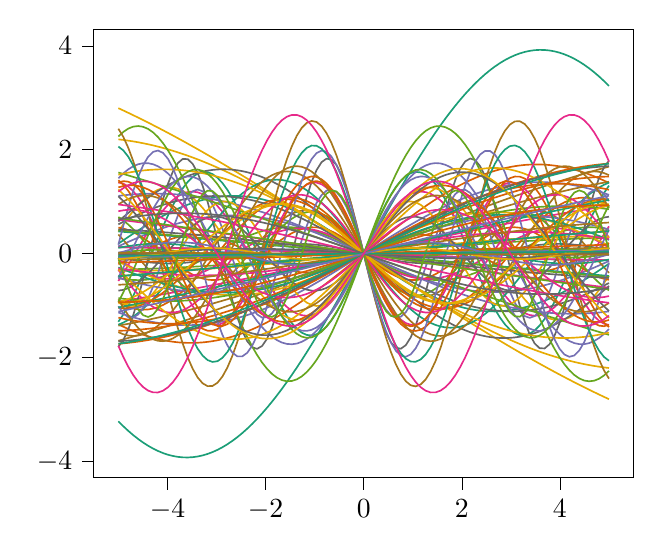
\begin{tikzpicture}

\definecolor{chocolate217952}{RGB}{217,95,2}
\definecolor{darkcyan27158119}{RGB}{27,158,119}
\definecolor{darkgoldenrod16611829}{RGB}{166,118,29}
\definecolor{darkgray176}{RGB}{176,176,176}
\definecolor{deeppink23141138}{RGB}{231,41,138}
\definecolor{dimgray102}{RGB}{102,102,102}
\definecolor{lightslategray117112179}{RGB}{117,112,179}
\definecolor{olivedrab10216630}{RGB}{102,166,30}
\definecolor{orange2301712}{RGB}{230,171,2}

\begin{axis}[
tick align=outside,
tick pos=left,
x grid style={darkgray176},
xmin=-5.5, xmax=5.5,
xtick style={color=black},
y grid style={darkgray176},
ymin=-4.31381980850293, ymax=4.31381980850293,
ytick style={color=black}
]
\addplot [semithick, darkcyan27158119]
table {%
-5 -1.31023422843018
-4.8989898989899 -1.16847120107245
-4.7979797979798 -1.001574530712
-4.6969696969697 -0.813134140084892
-4.5959595959596 -0.607203354169082
-4.49494949494949 -0.388211713762604
-4.39393939393939 -0.160869696715065
-4.29292929292929 0.0699326037553598
-4.19191919191919 0.29923066424501
-4.09090909090909 0.522092317330097
-3.98989898989899 0.733723841759725
-3.88888888888889 0.929573074692177
-3.78787878787879 1.10542732804549
-3.68686868686869 1.25750400279604
-3.58585858585859 1.38253195212507
-3.48484848484848 1.47782184330368
-3.38383838383838 1.5413240048428
-3.28282828282828 1.57167251462422
-3.18181818181818 1.56821458068369
-3.08080808080808 1.53102458266971
-2.97979797979798 1.46090247194819
-2.87878787878788 1.35935656476678
-2.77777777777778 1.22857109859504
-2.67676767676768 1.071359249499
-2.57575757575758 0.891102621139366
-2.47474747474747 0.691678506976099
-2.37373737373737 0.477376490258588
-2.27272727272727 0.252806175723346
-2.17171717171717 0.0227980376767631
-2.07070707070707 -0.207700482793968
-1.96969696969697 -0.433731396548123
-1.86868686868687 -0.650432812005778
-1.76767676767677 -0.853143513717806
-1.66666666666667 -1.03750322442193
-1.56565656565657 -1.19954639396281
-1.46464646464646 -1.33578749769034
-1.36363636363636 -1.44329600958023
-1.26262626262626 -1.51975943741605
-1.16161616161616 -1.56353306415538
-1.06060606060606 -1.57367532555051
-0.959595959595959 -1.5499680630564
-0.858585858585859 -1.49292121638878
-0.757575757575758 -1.40376185479611
-0.656565656565657 -1.28440778298132
-0.555555555555555 -1.13742628940572
-0.454545454545455 -0.965978924293363
-0.353535353535354 -0.773753495152501
-0.252525252525253 -0.564884742580625
-0.151515151515151 -0.343865402604729
-0.0505050505050502 -0.11544956859276
0.0505050505050502 0.11544956859276
0.151515151515151 0.343865402604729
0.252525252525253 0.564884742580625
0.353535353535354 0.773753495152501
0.454545454545454 0.965978924293362
0.555555555555555 1.13742628940572
0.656565656565657 1.28440778298132
0.757575757575758 1.40376185479611
0.858585858585858 1.49292121638878
0.959595959595959 1.5499680630564
1.06060606060606 1.57367532555051
1.16161616161616 1.56353306415538
1.26262626262626 1.51975943741605
1.36363636363636 1.44329600958023
1.46464646464646 1.33578749769034
1.56565656565657 1.19954639396281
1.66666666666667 1.03750322442193
1.76767676767677 0.853143513717807
1.86868686868687 0.650432812005779
1.96969696969697 0.433731396548123
2.07070707070707 0.207700482793968
2.17171717171717 -0.0227980376767617
2.27272727272727 -0.252806175723345
2.37373737373737 -0.477376490258588
2.47474747474747 -0.691678506976099
2.57575757575758 -0.891102621139365
2.67676767676768 -1.071359249499
2.77777777777778 -1.22857109859504
2.87878787878788 -1.35935656476678
2.97979797979798 -1.46090247194819
3.08080808080808 -1.53102458266971
3.18181818181818 -1.56821458068369
3.28282828282828 -1.57167251462422
3.38383838383838 -1.5413240048428
3.48484848484848 -1.47782184330368
3.58585858585859 -1.38253195212507
3.68686868686869 -1.25750400279604
3.78787878787879 -1.10542732804549
3.88888888888889 -0.929573074692176
3.98989898989899 -0.733723841759725
4.09090909090909 -0.522092317330098
4.19191919191919 -0.29923066424501
4.29292929292929 -0.0699326037553612
4.39393939393939 0.160869696715068
4.49494949494949 0.388211713762604
4.5959595959596 0.607203354169081
4.6969696969697 0.813134140084892
4.7979797979798 1.001574530712
4.8989898989899 1.16847120107246
5 1.31023422843018
};
\addplot [semithick, chocolate217952]
table {%
-5 -1.36044469182011
-4.8989898989899 -1.40621236743836
-4.7979797979798 -1.44913359196681
-4.6969696969697 -1.4891214843844
-4.5959595959596 -1.52609510131259
-4.49494949494949 -1.55997960086075
-4.39393939393939 -1.59070639412091
-4.29292929292929 -1.61821328400522
-4.19191919191919 -1.6424445911451
-4.09090909090909 -1.66335126659731
-3.98989898989899 -1.68089099112863
-3.88888888888889 -1.69502826087836
-3.78787878787879 -1.70573445922512
-3.68686868686869 -1.71298791471257
-3.58585858585859 -1.71677394491666
-3.48484848484848 -1.71708488616576
-3.38383838383838 -1.7139201090535
-3.28282828282828 -1.70728601971273
-3.18181818181818 -1.6971960468483
-3.08080808080808 -1.68367061455468
-2.97979797979798 -1.66673710097362
-2.87878787878788 -1.64642978287532
-2.77777777777778 -1.62278976627552
-2.67676767676768 -1.59586490322887
-2.57575757575758 -1.56570969496683
-2.47474747474747 -1.53238518157654
-2.37373737373737 -1.49595881844358
-2.27272727272727 -1.45650433970899
-2.17171717171717 -1.41410160901684
-2.07070707070707 -1.36883645785444
-1.96969696969697 -1.32080051181253
-1.86868686868687 -1.27009100511698
-1.76767676767677 -1.21681058380756
-1.66666666666667 -1.16106709796211
-1.56565656565657 -1.10297338338675
-1.46464646464646 -1.04264703321392
-1.36363636363636 -0.9802101598707
-1.26262626262626 -0.915789147899207
-1.16161616161616 -0.849514398129342
-1.06060606060606 -0.781520063721807
-0.959595959595959 -0.711943778615652
-0.858585858585859 -0.640926378930053
-0.757575757575758 -0.56861161788423
-0.656565656565657 -0.495145874812596
-0.555555555555555 -0.420677858864117
-0.454545454545455 -0.345358307985679
-0.353535353535354 -0.269339683798757
-0.252525252525253 -0.192775862987039
-0.151515151515151 -0.115821825819676
-0.0505050505050502 -0.03863334244066
0.0505050505050502 0.03863334244066
0.151515151515151 0.115821825819676
0.252525252525253 0.192775862987039
0.353535353535354 0.269339683798757
0.454545454545454 0.345358307985678
0.555555555555555 0.420677858864117
0.656565656565657 0.495145874812596
0.757575757575758 0.56861161788423
0.858585858585858 0.640926378930052
0.959595959595959 0.711943778615652
1.06060606060606 0.781520063721807
1.16161616161616 0.849514398129342
1.26262626262626 0.915789147899206
1.36363636363636 0.980210159870699
1.46464646464646 1.04264703321392
1.56565656565657 1.10297338338675
1.66666666666667 1.16106709796211
1.76767676767677 1.21681058380756
1.86868686868687 1.27009100511698
1.96969696969697 1.32080051181253
2.07070707070707 1.36883645785444
2.17171717171717 1.41410160901684
2.27272727272727 1.45650433970899
2.37373737373737 1.49595881844358
2.47474747474747 1.53238518157654
2.57575757575758 1.56570969496683
2.67676767676768 1.59586490322887
2.77777777777778 1.62278976627552
2.87878787878788 1.64642978287532
2.97979797979798 1.66673710097362
3.08080808080808 1.68367061455469
3.18181818181818 1.6971960468483
3.28282828282828 1.70728601971273
3.38383838383838 1.7139201090535
3.48484848484848 1.71708488616576
3.58585858585859 1.71677394491666
3.68686868686869 1.71298791471257
3.78787878787879 1.70573445922512
3.88888888888889 1.69502826087836
3.98989898989899 1.68089099112863
4.09090909090909 1.66335126659731
4.19191919191919 1.6424445911451
4.29292929292929 1.61821328400522
4.39393939393939 1.59070639412091
4.49494949494949 1.55997960086075
4.5959595959596 1.52609510131259
4.6969696969697 1.4891214843844
4.7979797979798 1.44913359196681
4.8989898989899 1.40621236743836
5 1.36044469182011
};
\addplot [semithick, lightslategray117112179]
table {%
-5 0.14182954839444
-4.8989898989899 0.18467269002218
-4.7979797979798 0.226860952221281
-4.6969696969697 0.268244728544571
-4.5959595959596 0.308677265382784
-4.49494949494949 0.348015182376757
-4.39393939393939 0.386118980867528
-4.29292929292929 0.422853538581299
-4.19191919191919 0.458088588795013
-4.09090909090909 0.491699182283373
-3.98989898989899 0.523566130409136
-3.88888888888889 0.553576427785426
-3.78787878787879 0.581623653011243
-3.68686868686869 0.607608346059071
-3.58585858585859 0.631438360976336
-3.48484848484848 0.653029192649956
-3.38383838383838 0.672304276475233
-3.28282828282828 0.689195259866406
-3.18181818181818 0.70364224464605
-3.08080808080808 0.715593999453768
-2.97979797979798 0.725008141420935
-2.87878787878788 0.731851286467255
-2.77777777777778 0.736099167686139
-2.67676767676768 0.737736721399112
-2.57575757575758 0.73675814057407
-2.47474747474747 0.733166895417958
-2.37373737373737 0.726975721070853
-2.27272727272727 0.718206572445085
-2.17171717171717 0.706890546369541
-2.07070707070707 0.693067771315246
-1.96969696969697 0.676787265093273
-1.86868686868687 0.658106761029601
-1.76767676767677 0.637092503233343
-1.66666666666667 0.613819011684346
-1.56565656565657 0.588368817973211
-1.46464646464646 0.560832172630834
-1.36363636363636 0.531306725085324
-1.26262626262626 0.499897177381238
-1.16161616161616 0.466714912889077
-1.06060606060606 0.43187760132172
-0.959595959595959 0.395508781458463
-0.858585858585859 0.35773742305639
-0.757575757575758 0.318697469502616
-0.656565656565657 0.278527362829227
-0.555555555555555 0.23736955277529
-0.454545454545455 0.195369991636887
-0.353535353535354 0.152677616696503
-0.252525252525253 0.109443822067176
-0.151515151515151 0.0658219218243188
-0.0505050505050502 0.021966606329044
0.0505050505050502 -0.021966606329044
0.151515151515151 -0.0658219218243188
0.252525252525253 -0.109443822067176
0.353535353535354 -0.152677616696503
0.454545454545454 -0.195369991636887
0.555555555555555 -0.23736955277529
0.656565656565657 -0.278527362829227
0.757575757575758 -0.318697469502616
0.858585858585858 -0.35773742305639
0.959595959595959 -0.395508781458463
1.06060606060606 -0.43187760132172
1.16161616161616 -0.466714912889077
1.26262626262626 -0.499897177381238
1.36363636363636 -0.531306725085324
1.46464646464646 -0.560832172630834
1.56565656565657 -0.588368817973211
1.66666666666667 -0.613819011684346
1.76767676767677 -0.637092503233343
1.86868686868687 -0.658106761029601
1.96969696969697 -0.676787265093273
2.07070707070707 -0.693067771315246
2.17171717171717 -0.706890546369541
2.27272727272727 -0.718206572445085
2.37373737373737 -0.726975721070853
2.47474747474747 -0.733166895417958
2.57575757575758 -0.73675814057407
2.67676767676768 -0.737736721399112
2.77777777777778 -0.736099167686139
2.87878787878788 -0.731851286467255
2.97979797979798 -0.725008141420935
3.08080808080808 -0.715593999453768
3.18181818181818 -0.70364224464605
3.28282828282828 -0.689195259866406
3.38383838383838 -0.672304276475233
3.48484848484848 -0.653029192649956
3.58585858585859 -0.631438360976336
3.68686868686869 -0.607608346059071
3.78787878787879 -0.581623653011243
3.88888888888889 -0.553576427785426
3.98989898989899 -0.523566130409136
4.09090909090909 -0.491699182283373
4.19191919191919 -0.458088588795013
4.29292929292929 -0.422853538581299
4.39393939393939 -0.386118980867528
4.49494949494949 -0.348015182376757
4.5959595959596 -0.308677265382784
4.6969696969697 -0.268244728544571
4.7979797979798 -0.226860952221281
4.8989898989899 -0.184672690022179
5 -0.14182954839444
};
\addplot [semithick, deeppink23141138]
table {%
-5 -0.52575000735024
-4.8989898989899 -0.375300020112409
-4.7979797979798 -0.217904987406914
-4.6969696969697 -0.0564775540510872
-4.5959595959596 0.105995014289466
-4.49494949494949 0.266506111395977
-4.39393939393939 0.422085428694693
-4.29292929292929 0.569853921755655
-4.19191919191919 0.707077087919664
-4.09090909090909 0.831215569134084
-3.98989898989899 0.939972143576057
-3.88888888888889 1.03133423646826
-3.78787878787879 1.10361116341114
-3.68686868686869 1.15546541703198
-3.58585858585859 1.18593741798149
-3.48484848484848 1.19446327225289
-3.38383838383838 1.1808852062187
-3.28282828282828 1.14545448628157
-3.18181818181818 1.08882676911012
-3.08080808080808 1.01204996850507
-2.97979797979798 0.91654486342321
-2.87878787878788 0.804078806013877
-2.77777777777778 0.676733016208903
-2.67676767676768 0.53686406809013
-2.57575757575758 0.387060280741335
-2.47474747474747 0.230093820585675
-2.37373737373737 0.0688694015700138
-2.27272727272727 -0.0936294674845546
-2.17171717171717 -0.254395693656241
-2.07070707070707 -0.410454247127321
-1.96969696969697 -0.558917215051027
-1.86868686868687 -0.697037243291365
-1.76767676767677 -0.822258377079571
-1.66666666666667 -0.932263359764789
-1.56565656565657 -1.02501651438066
-1.46464646464646 -1.09880141449084
-1.36363636363636 -1.15225264720264
-1.26262626262626 -1.18438108056405
-1.16161616161616 -1.19459216776306
-1.06060606060606 -1.18269694940433
-0.959595959595959 -1.1489155502625
-0.858585858585859 -1.09387310580369
-0.757575757575758 -1.0185881938561
-0.656565656565657 -0.924453985505492
-0.555555555555555 -0.813212464023982
-0.454545454545455 -0.686922188919103
-0.353535353535354 -0.547920201639625
-0.252525252525253 -0.398778777885033
-0.151515151515151 -0.242257826830865
-0.0505050505050502 -0.0812538181372825
0.0505050505050502 0.0812538181372825
0.151515151515151 0.242257826830865
0.252525252525253 0.398778777885033
0.353535353535354 0.547920201639625
0.454545454545454 0.686922188919102
0.555555555555555 0.813212464023982
0.656565656565657 0.924453985505492
0.757575757575758 1.0185881938561
0.858585858585858 1.09387310580369
0.959595959595959 1.1489155502625
1.06060606060606 1.18269694940433
1.16161616161616 1.19459216776306
1.26262626262626 1.18438108056405
1.36363636363636 1.15225264720264
1.46464646464646 1.09880141449084
1.56565656565657 1.02501651438066
1.66666666666667 0.932263359764789
1.76767676767677 0.822258377079572
1.86868686868687 0.697037243291366
1.96969696969697 0.558917215051027
2.07070707070707 0.410454247127321
2.17171717171717 0.254395693656242
2.27272727272727 0.0936294674845551
2.37373737373737 -0.0688694015700138
2.47474747474747 -0.230093820585675
2.57575757575758 -0.387060280741334
2.67676767676768 -0.536864068090129
2.77777777777778 -0.676733016208903
2.87878787878788 -0.804078806013877
2.97979797979798 -0.91654486342321
3.08080808080808 -1.01204996850507
3.18181818181818 -1.08882676911012
3.28282828282828 -1.14545448628157
3.38383838383838 -1.1808852062187
3.48484848484848 -1.19446327225289
3.58585858585859 -1.18593741798149
3.68686868686869 -1.15546541703198
3.78787878787879 -1.10361116341115
3.88888888888889 -1.03133423646826
3.98989898989899 -0.939972143576057
4.09090909090909 -0.831215569134084
4.19191919191919 -0.707077087919664
4.29292929292929 -0.569853921755657
4.39393939393939 -0.422085428694691
4.49494949494949 -0.266506111395977
4.5959595959596 -0.105995014289468
4.6969696969697 0.0564775540510872
4.7979797979798 0.217904987406914
4.8989898989899 0.37530002011241
5 0.52575000735024
};
\addplot [semithick, olivedrab10216630]
table {%
-5 -0.467170418478261
-4.8989898989899 -0.485538533547572
-4.7979797979798 -0.49871541556784
-4.6969696969697 -0.506560181250303
-4.5959595959596 -0.508988956702244
-4.49494949494949 -0.505975774181611
-4.39393939393939 -0.497552849736366
-4.29292929292929 -0.483810238760116
-4.19191919191919 -0.464894873146729
-4.09090909090909 -0.44100899033839
-3.98989898989899 -0.412407971063245
-3.88888888888889 -0.379397608880895
-3.78787878787879 -0.342330840728951
-3.68686868686869 -0.301603973426659
-3.58585858585859 -0.257652446480701
-3.48484848484848 -0.210946176495989
-3.38383838383838 -0.161984532967607
-3.28282828282828 -0.111290999171255
-3.18181818181818 -0.0594075752363444
-3.08080808080808 -0.00688898324241846
-2.97979797979798 0.0457032637037129
-2.87878787878788 0.0978068649984799
-2.77777777777778 0.148864744491738
-2.67676767676768 0.198331006578657
-2.57575757575758 0.245676772752556
-2.47474747474747 0.290395836216009
-2.37373737373737 0.332010074092799
-2.27272727272727 0.370074559374975
-2.17171717171717 0.404182317949591
-2.07070707070707 0.433968679844424
-1.96969696969697 0.459115178170454
-1.86868686868687 0.479352954074759
-1.76767676767677 0.494465631299115
-1.66666666666667 0.504291629610345
-1.56565656565657 0.508725892367938
-1.46464646464646 0.507721009758286
-1.36363636363636 0.501287725686256
-1.26262626262626 0.489494822904565
-1.16161616161616 0.472468387609129
-1.06060606060606 0.45039046136309
-0.959595959595959 0.423497094762773
-0.858585858585859 0.39207582365518
-0.757575757575758 0.356462594890554
-0.656565656565657 0.317038174478947
-0.555555555555555 0.274224076553717
-0.454545454545455 0.228478056668252
-0.353535353535354 0.180289217610246
-0.252525252525253 0.130172780060713
-0.151515151515151 0.0786645740082768
-0.0505050505050502 0.0263153098149001
0.0505050505050502 -0.0263153098149001
0.151515151515151 -0.0786645740082768
0.252525252525253 -0.130172780060713
0.353535353535354 -0.180289217610246
0.454545454545454 -0.228478056668252
0.555555555555555 -0.274224076553717
0.656565656565657 -0.317038174478947
0.757575757575758 -0.356462594890554
0.858585858585858 -0.39207582365518
0.959595959595959 -0.423497094762773
1.06060606060606 -0.45039046136309
1.16161616161616 -0.472468387609129
1.26262626262626 -0.489494822904565
1.36363636363636 -0.501287725686255
1.46464646464646 -0.507721009758286
1.56565656565657 -0.508725892367938
1.66666666666667 -0.504291629610345
1.76767676767677 -0.494465631299115
1.86868686868687 -0.479352954074759
1.96969696969697 -0.459115178170454
2.07070707070707 -0.433968679844424
2.17171717171717 -0.404182317949591
2.27272727272727 -0.370074559374976
2.37373737373737 -0.332010074092799
2.47474747474747 -0.290395836216009
2.57575757575758 -0.245676772752556
2.67676767676768 -0.198331006578657
2.77777777777778 -0.148864744491738
2.87878787878788 -0.0978068649984799
2.97979797979798 -0.0457032637037131
3.08080808080808 0.00688898324241869
3.18181818181818 0.0594075752363444
3.28282828282828 0.111290999171255
3.38383838383838 0.161984532967607
3.48484848484848 0.210946176495989
3.58585858585859 0.257652446480702
3.68686868686869 0.301603973426659
3.78787878787879 0.342330840728951
3.88888888888889 0.379397608880895
3.98989898989899 0.412407971063245
4.09090909090909 0.44100899033839
4.19191919191919 0.464894873146729
4.29292929292929 0.483810238760116
4.39393939393939 0.497552849736366
4.49494949494949 0.505975774181611
4.5959595959596 0.508988956702244
4.6969696969697 0.506560181250303
4.7979797979798 0.49871541556784
4.8989898989899 0.485538533547572
5 0.467170418478261
};
\addplot [semithick, orange2301712]
table {%
-5 2.19996153878231
-4.8989898989899 2.18853999326829
-4.7979797979798 2.17535936838932
-4.6969696969697 2.16043025831564
-4.5959595959596 2.14376466259467
-4.49494949494949 2.12537597650621
-4.39393939393939 2.10527898029569
-4.29292929292929 2.0834898272943
-4.19191919191919 2.06002603093545
-4.09090909090909 2.03490645067801
-3.98989898989899 2.00815127684769
-3.88888888888889 1.97978201440867
-3.78787878787879 1.94982146567864
-3.68686868686869 1.91829371200094
-3.58585858585859 1.88522409438881
-3.48484848484848 1.85063919315703
-3.38383838383838 1.81456680655754
-3.28282828282828 1.77703592843604
-3.18181818181818 1.73807672492772
-3.08080808080808 1.69772051021059
-2.97979797979798 1.65599972133619
-2.87878787878788 1.6129478921577
-2.77777777777778 1.56859962637647
-2.67676767676768 1.52299056972867
-2.57575757575758 1.47615738133439
-2.47474747474747 1.42813770423215
-2.37373737373737 1.37897013512267
-2.27272727272727 1.328694193346
-2.17171717171717 1.27735028911718
-2.07070707070707 1.22497969104575
-1.96969696969697 1.17162449296535
-1.86868686868687 1.11732758010003
-1.76767676767677 1.06213259459447
-1.66666666666667 1.00608390043577
-1.56565656565657 0.94922654779511
-1.46464646464646 0.891606236817833
-1.36363636363636 0.833269280891106
-1.26262626262626 0.774262569418687
-1.16161616161616 0.7146335301327
-1.06060606060606 0.654430090972724
-0.959595959595959 0.593700641562821
-0.858585858585859 0.532493994317494
-0.757575757575758 0.470859345207798
-0.656565656565657 0.408846234219181
-0.555555555555555 0.3465045055328
-0.454545454545455 0.283884267462346
-0.353535353535354 0.221035852178562
-0.252525252525253 0.158009775253831
-0.151515151515151 0.0948566950593565
-0.0505050505050502 0.0316273720475614
0.0505050505050502 -0.0316273720475614
0.151515151515151 -0.0948566950593565
0.252525252525253 -0.158009775253831
0.353535353535354 -0.221035852178562
0.454545454545454 -0.283884267462346
0.555555555555555 -0.3465045055328
0.656565656565657 -0.408846234219181
0.757575757575758 -0.470859345207798
0.858585858585858 -0.532493994317493
0.959595959595959 -0.593700641562821
1.06060606060606 -0.654430090972724
1.16161616161616 -0.7146335301327
1.26262626262626 -0.774262569418686
1.36363636363636 -0.833269280891106
1.46464646464646 -0.891606236817833
1.56565656565657 -0.94922654779511
1.66666666666667 -1.00608390043577
1.76767676767677 -1.06213259459447
1.86868686868687 -1.11732758010003
1.96969696969697 -1.17162449296535
2.07070707070707 -1.22497969104575
2.17171717171717 -1.27735028911718
2.27272727272727 -1.328694193346
2.37373737373737 -1.37897013512267
2.47474747474747 -1.42813770423215
2.57575757575758 -1.47615738133439
2.67676767676768 -1.52299056972867
2.77777777777778 -1.56859962637647
2.87878787878788 -1.6129478921577
2.97979797979798 -1.65599972133619
3.08080808080808 -1.69772051021059
3.18181818181818 -1.73807672492772
3.28282828282828 -1.77703592843604
3.38383838383838 -1.81456680655754
3.48484848484848 -1.85063919315703
3.58585858585859 -1.88522409438881
3.68686868686869 -1.91829371200094
3.78787878787879 -1.94982146567864
3.88888888888889 -1.97978201440867
3.98989898989899 -2.00815127684769
4.09090909090909 -2.03490645067801
4.19191919191919 -2.06002603093545
4.29292929292929 -2.0834898272943
4.39393939393939 -2.10527898029569
4.49494949494949 -2.12537597650621
4.5959595959596 -2.14376466259467
4.6969696969697 -2.16043025831564
4.7979797979798 -2.17535936838932
4.8989898989899 -2.18853999326829
5 -2.19996153878231
};
\addplot [semithick, darkgoldenrod16611829]
table {%
-5 0.36883155284084
-4.8989898989899 0.263617147373229
-4.7979797979798 0.153522441092125
-4.6969696969697 0.0405855991547606
-4.5959595959596 -0.073102597292526
-4.49494949494949 -0.185437457401148
-4.39393939393939 -0.294339344415171
-4.29292929292929 -0.397792175643916
-4.19191919191919 -0.493880745868624
-4.09090909090909 -0.580826183221102
-3.98989898989899 -0.657018881145522
-3.88888888888889 -0.721048296779373
-3.78787878787879 -0.771729064101063
-3.68686868686869 -0.808122938415763
-3.58585858585859 -0.829556165924853
-3.48484848484848 -0.835631956818981
-3.38383838383838 -0.826237830982422
-3.28282828282828 -0.801547700318932
-3.18181818181818 -0.762018649149326
-3.08080808080808 -0.708382472284762
-2.97979797979798 -0.641632127429974
-2.87878787878788 -0.563003352720899
-2.77777777777778 -0.473951789708173
-2.67676767676768 -0.376126035304951
-2.57575757575758 -0.271337121583886
-2.47474747474747 -0.161524988438775
-2.37373737373737 -0.0487225697969429
-2.27272727272727 0.0649818417515907
-2.17171717171717 0.177483255170744
-2.07070707070707 0.286698950330588
-1.96969696969697 0.390607035061945
-1.86868686868687 0.487283876112973
-1.76767676767677 0.574939711054601
-1.66666666666667 0.651951781857483
-1.56565656565657 0.716894376744017
-1.46464646464646 0.768565224155569
-1.36363636363636 0.80600775020774
-1.26262626262626 0.82852878758508
-1.16161616161616 0.835711408033382
-1.06060606060606 0.827422640883756
-0.959595959595959 0.803815934716716
-0.858585858585859 0.765328316593887
-0.757575757575758 0.712672301448027
-0.656565656565657 0.646822701411473
-0.555555555555555 0.568998579279757
-0.454545454545455 0.480640680202932
-0.353535353535354 0.383384759407998
-0.252525252525253 0.279031299731913
-0.151515151515151 0.169512179579485
-0.0505050505050502 0.0568549083767868
0.0505050505050502 -0.0568549083767868
0.151515151515151 -0.169512179579485
0.252525252525253 -0.279031299731913
0.353535353535354 -0.383384759407998
0.454545454545454 -0.480640680202931
0.555555555555555 -0.568998579279757
0.656565656565657 -0.646822701411473
0.757575757575758 -0.712672301448027
0.858585858585858 -0.765328316593887
0.959595959595959 -0.803815934716716
1.06060606060606 -0.827422640883756
1.16161616161616 -0.835711408033382
1.26262626262626 -0.82852878758508
1.36363636363636 -0.80600775020774
1.46464646464646 -0.768565224155569
1.56565656565657 -0.716894376744017
1.66666666666667 -0.651951781857483
1.76767676767677 -0.574939711054601
1.86868686868687 -0.487283876112973
1.96969696969697 -0.390607035061945
2.07070707070707 -0.286698950330588
2.17171717171717 -0.177483255170745
2.27272727272727 -0.0649818417515911
2.37373737373737 0.0487225697969429
2.47474747474747 0.161524988438775
2.57575757575758 0.271337121583886
2.67676767676768 0.37612603530495
2.77777777777778 0.473951789708173
2.87878787878788 0.563003352720899
2.97979797979798 0.641632127429973
3.08080808080808 0.708382472284762
3.18181818181818 0.762018649149326
3.28282828282828 0.801547700318932
3.38383838383838 0.826237830982422
3.48484848484848 0.835631956818981
3.58585858585859 0.829556165924853
3.68686868686869 0.808122938415763
3.78787878787879 0.771729064101063
3.88888888888889 0.721048296779373
3.98989898989899 0.657018881145522
4.09090909090909 0.580826183221103
4.19191919191919 0.493880745868624
4.29292929292929 0.397792175643917
4.39393939393939 0.29433934441517
4.49494949494949 0.185437457401148
4.5959595959596 0.0731025972925267
4.6969696969697 -0.0405855991547606
4.7979797979798 -0.153522441092125
4.8989898989899 -0.263617147373231
5 -0.36883155284084
};
\addplot [semithick, dimgray102]
table {%
-5 0.124369150306977
-4.8989898989899 0.123629700869409
-4.7979797979798 0.122795156531711
-4.6969696969697 0.121866159218194
-4.5959595959596 0.120843423505582
-4.49494949494949 0.119727736073369
-4.39393939393939 0.118519955098709
-4.29292929292929 0.117221009596317
-4.19191919191919 0.115831898703875
-4.09090909090909 0.114353690913507
-3.98989898989899 0.112787523249901
-3.88888888888889 0.111134600395722
-3.78787878787879 0.109396193764981
-3.68686868686869 0.107573640525072
-3.58585858585859 0.105668342568235
-3.48484848484848 0.103681765433234
-3.38383838383838 0.101615437178074
-3.28282828282828 0.0994709472046375
-3.18181818181818 0.0972499450361237
-3.08080808080808 0.0949541390482542
-2.97979797979798 0.0925852951552035
-2.87878787878788 0.0901452354512729
-2.77777777777778 0.0876358368093514
-2.67676767676768 0.0850590294372418
-2.57575757575758 0.0824167953929605
-2.47474747474747 0.0797111670601564
-2.37373737373737 0.0769442255848186
-2.27272727272727 0.0741180992744769
-2.17171717171717 0.071234961961126
-2.07070707070707 0.0682970313291324
-1.96969696969697 0.0653065672094111
-1.86868686868687 0.0622658698411831
-1.76767676767677 0.0591772781026509
-1.66666666666667 0.0560431677119539
-1.56565656565657 0.0528659493997863
-1.46464646464646 0.0496480670550837
-1.36363636363636 0.0463919958452054
-1.26262626262626 0.043100240312056
-1.16161616161616 0.0397753324456145
-1.06060606060606 0.0364198297363485
-0.959595959595959 0.033036313208015
-0.858585858585859 0.0296273854323594
-0.757575757575758 0.026195668527239
-0.656565656565657 0.0227438021397134
-0.555555555555555 0.0192744414156503
-0.454545454545455 0.0157902549574102
-0.353535353535354 0.0122939227711804
-0.252525252525253 0.00878813420553777
-0.151515151515151 0.00527558588282439
-0.0505050505050502 0.00175897962492939
0.0505050505050502 -0.00175897962492939
0.151515151515151 -0.00527558588282439
0.252525252525253 -0.00878813420553777
0.353535353535354 -0.0122939227711804
0.454545454545454 -0.0157902549574102
0.555555555555555 -0.0192744414156503
0.656565656565657 -0.0227438021397134
0.757575757575758 -0.026195668527239
0.858585858585858 -0.0296273854323593
0.959595959595959 -0.033036313208015
1.06060606060606 -0.0364198297363485
1.16161616161616 -0.0397753324456145
1.26262626262626 -0.043100240312056
1.36363636363636 -0.0463919958452053
1.46464646464646 -0.0496480670550837
1.56565656565657 -0.0528659493997863
1.66666666666667 -0.0560431677119539
1.76767676767677 -0.0591772781026509
1.86868686868687 -0.0622658698411831
1.96969696969697 -0.0653065672094111
2.07070707070707 -0.0682970313291324
2.17171717171717 -0.071234961961126
2.27272727272727 -0.0741180992744769
2.37373737373737 -0.0769442255848186
2.47474747474747 -0.0797111670601564
2.57575757575758 -0.0824167953929604
2.67676767676768 -0.0850590294372418
2.77777777777778 -0.0876358368093514
2.87878787878788 -0.0901452354512729
2.97979797979798 -0.0925852951552035
3.08080808080808 -0.0949541390482542
3.18181818181818 -0.0972499450361237
3.28282828282828 -0.0994709472046375
3.38383838383838 -0.101615437178074
3.48484848484848 -0.103681765433234
3.58585858585859 -0.105668342568235
3.68686868686869 -0.107573640525072
3.78787878787879 -0.109396193764981
3.88888888888889 -0.111134600395722
3.98989898989899 -0.112787523249901
4.09090909090909 -0.114353690913507
4.19191919191919 -0.115831898703875
4.29292929292929 -0.117221009596317
4.39393939393939 -0.118519955098709
4.49494949494949 -0.119727736073369
4.5959595959596 -0.120843423505582
4.6969696969697 -0.121866159218194
4.7979797979798 -0.122795156531711
4.8989898989899 -0.123629700869409
5 -0.124369150306977
};
\addplot [semithick, darkcyan27158119]
table {%
-5 0.192107306885827
-4.8989898989899 0.257370863618842
-4.7979797979798 0.321709468939234
-4.6969696969697 0.384891899766656
-4.5959595959596 0.446691088134575
-4.49494949494949 0.50688493723772
-4.39393939393939 0.565257119613936
-4.29292929292929 0.621597854591907
-4.19191919191919 0.67570466221072
-4.09090909090909 0.727383090901786
-3.98989898989899 0.77644741631796
-3.88888888888889 0.822721308798358
-3.78787878787879 0.866038467070119
-3.68686868686869 0.906243215909672
-3.58585858585859 0.943191065615619
-3.48484848484848 0.976749231282556
-3.38383838383838 1.00679711000966
-3.28282828282828 1.03322671432904
-3.18181818181818 1.05594306029608
-3.08080808080808 1.07486450884725
-2.97979797979798 1.08992305919829
-2.87878787878788 1.10106459322867
-2.77777777777778 1.1082490699738
-2.67676767676768 1.11145066952608
-2.57575757575758 1.11065788582773
-2.47474747474747 1.10587356802178
-2.37373737373737 1.09711491021268
-2.27272727272727 1.08441338967335
-2.17171717171717 1.06781465372065
-2.07070707070707 1.04737835566597
-1.96969696969697 1.02317794043034
-1.86868686868687 0.995300380594653
-1.76767676767677 0.963845863833577
-1.66666666666667 0.928927432856383
-1.56565656565657 0.8906705791488
-1.46464646464646 0.849212791975858
-1.36363636363636 0.804703064266558
-1.26262626262626 0.757301357156133
-1.16161616161616 0.707178025110258
-1.06060606060606 0.654513203697232
-0.959595959595959 0.599496162208366
-0.858585858585859 0.542324623453182
-0.757575757575758 0.483204053173953
-0.656565656565657 0.422346921633345
-0.555555555555555 0.359971940028867
-0.454545454545455 0.29630327447838
-0.353535353535354 0.231569740401439
-0.252525252525253 0.166003980191775
-0.151515151515151 0.099841627136206
-0.0505050505050502 0.0333204585847421
0.0505050505050502 -0.0333204585847421
0.151515151515151 -0.099841627136206
0.252525252525253 -0.166003980191775
0.353535353535354 -0.231569740401439
0.454545454545454 -0.296303274478379
0.555555555555555 -0.359971940028867
0.656565656565657 -0.422346921633345
0.757575757575758 -0.483204053173953
0.858585858585858 -0.542324623453181
0.959595959595959 -0.599496162208366
1.06060606060606 -0.654513203697232
1.16161616161616 -0.707178025110258
1.26262626262626 -0.757301357156133
1.36363636363636 -0.804703064266558
1.46464646464646 -0.849212791975858
1.56565656565657 -0.8906705791488
1.66666666666667 -0.928927432856383
1.76767676767677 -0.963845863833577
1.86868686868687 -0.995300380594653
1.96969696969697 -1.02317794043034
2.07070707070707 -1.04737835566597
2.17171717171717 -1.06781465372065
2.27272727272727 -1.08441338967335
2.37373737373737 -1.09711491021268
2.47474747474747 -1.10587356802178
2.57575757575758 -1.11065788582773
2.67676767676768 -1.11145066952608
2.77777777777778 -1.1082490699738
2.87878787878788 -1.10106459322867
2.97979797979798 -1.08992305919829
3.08080808080808 -1.07486450884725
3.18181818181818 -1.05594306029608
3.28282828282828 -1.03322671432904
3.38383838383838 -1.00679711000966
3.48484848484848 -0.976749231282556
3.58585858585859 -0.943191065615619
3.68686868686869 -0.906243215909672
3.78787878787879 -0.866038467070119
3.88888888888889 -0.822721308798358
3.98989898989899 -0.77644741631796
4.09090909090909 -0.727383090901786
4.19191919191919 -0.67570466221072
4.29292929292929 -0.621597854591907
4.39393939393939 -0.565257119613935
4.49494949494949 -0.50688493723772
4.5959595959596 -0.446691088134576
4.6969696969697 -0.384891899766656
4.7979797979798 -0.321709468939234
4.8989898989899 -0.257370863618842
5 -0.192107306885827
};
\addplot [semithick, chocolate217952]
table {%
-5 -0.203910432785738
-4.8989898989899 -0.160102993147983
-4.7979797979798 -0.113210471272397
-4.6969696969697 -0.0641364560518615
-4.5959595959596 -0.0138265723602083
-4.49494949494949 0.0367497405340467
-4.39393939393939 0.0866179094421258
-4.29292929292929 0.134817006656767
-4.19191919191919 0.180418266414304
-4.09090909090909 0.222542981616671
-3.98989898989899 0.260379435954952
-3.88888888888889 0.293198545163285
-3.78787878787879 0.320367906006171
-3.68686868686869 0.341363982284181
-3.58585858585859 0.355782193041546
-3.48484848484848 0.363344708582305
-3.38383838383838 0.363905804070779
-3.28282828282828 0.357454667555915
-3.18181818181818 0.344115608310667
-3.08080808080808 0.324145661471842
-2.97979797979798 0.297929635137473
-2.87878787878788 0.265972695360989
-2.77777777777778 0.228890631924588
-2.67676767676768 0.187397992464142
-2.57575757575758 0.142294313593445
-2.47474747474747 0.0944487143452474
-2.37373737373737 0.0447831488035823
-2.27272727272727 -0.00574535936152481
-2.17171717171717 -0.0561631581278403
-2.07070707070707 -0.105498728772408
-1.96969696969697 -0.152801406415727
-1.86868686868687 -0.197159698725706
-1.76767676767677 -0.237718849791695
-1.66666666666667 -0.273697310723977
-1.56565656565657 -0.304401799600807
-1.46464646464646 -0.329240660567456
-1.36363636363636 -0.347735264665968
-1.26262626262626 -0.359529232708933
-1.16161616161616 -0.364395302478403
-1.06060606060606 -0.36223970792342
-0.959595959595959 -0.353103985971827
-0.858585858585859 -0.33716417614024
-0.757575757575758 -0.314727428365202
-0.656565656565657 -0.286226084420432
-0.555555555555555 -0.252209346967478
-0.454545454545455 -0.213332696771824
-0.353535353535354 -0.170345262007944
-0.252525252525253 -0.124075383038705
-0.151515151515151 -0.0754146508265725
-0.0505050505050502 -0.0253007265462426
0.0505050505050502 0.0253007265462426
0.151515151515151 0.0754146508265725
0.252525252525253 0.124075383038705
0.353535353535354 0.170345262007944
0.454545454545454 0.213332696771823
0.555555555555555 0.252209346967478
0.656565656565657 0.286226084420432
0.757575757575758 0.314727428365202
0.858585858585858 0.33716417614024
0.959595959595959 0.353103985971827
1.06060606060606 0.36223970792342
1.16161616161616 0.364395302478403
1.26262626262626 0.359529232708933
1.36363636363636 0.347735264665968
1.46464646464646 0.329240660567456
1.56565656565657 0.304401799600807
1.66666666666667 0.273697310723977
1.76767676767677 0.237718849791695
1.86868686868687 0.197159698725706
1.96969696969697 0.152801406415727
2.07070707070707 0.105498728772408
2.17171717171717 0.0561631581278405
2.27272727272727 0.00574535936152513
2.37373737373737 -0.0447831488035823
2.47474747474747 -0.0944487143452474
2.57575757575758 -0.142294313593445
2.67676767676768 -0.187397992464141
2.77777777777778 -0.228890631924588
2.87878787878788 -0.265972695360989
2.97979797979798 -0.297929635137473
3.08080808080808 -0.324145661471842
3.18181818181818 -0.344115608310667
3.28282828282828 -0.357454667555915
3.38383838383838 -0.363905804070779
3.48484848484848 -0.363344708582305
3.58585858585859 -0.355782193041546
3.68686868686869 -0.341363982284181
3.78787878787879 -0.320367906006171
3.88888888888889 -0.293198545163285
3.98989898989899 -0.260379435954952
4.09090909090909 -0.222542981616671
4.19191919191919 -0.180418266414304
4.29292929292929 -0.134817006656767
4.39393939393939 -0.0866179094421252
4.49494949494949 -0.0367497405340467
4.5959595959596 0.0138265723602079
4.6969696969697 0.0641364560518615
4.7979797979798 0.113210471272397
4.8989898989899 0.160102993147984
5 0.203910432785738
};
\addplot [semithick, lightslategray117112179]
table {%
-5 -1.13153764933796
-4.8989898989899 -1.16484667181074
-4.7979797979798 -1.1959050157868
-4.6969696969697 -1.22465267135359
-4.5959595959596 -1.25103409323481
-4.49494949494949 -1.27499830811324
-4.39393939393939 -1.29649901311962
-4.29292929292929 -1.31549466529765
-4.19191919191919 -1.3319485618718
-4.09090909090909 -1.34582891116332
-3.98989898989899 -1.357108894017
-3.88888888888889 -1.36576671562029
-3.78787878787879 -1.37178564761455
-3.68686868686869 -1.37515406041697
-3.58585858585859 -1.37586544569092
-3.48484848484848 -1.37391842892114
-3.38383838383838 -1.3693167720695
-3.28282828282828 -1.3620693663063
-3.18181818181818 -1.35219021483102
-3.08080808080808 -1.3396984058158
-2.97979797979798 -1.3246180755239
-2.87878787878788 -1.30697836167442
-2.77777777777778 -1.28681334714334
-2.67676767676768 -1.26416199410971
-2.57575757575758 -1.2390680687742
-2.47474747474747 -1.2115800567955
-2.37373737373737 -1.1817510696079
-2.27272727272727 -1.14963874180116
-2.17171717171717 -1.11530511976078
-2.07070707070707 -1.07881654178409
-1.96969696969697 -1.04024350990351
-1.86868686868687 -0.999660553664861
-1.76767676767677 -0.957146086123837
-1.66666666666667 -0.912782252338843
-1.56565656565657 -0.866654770653028
-1.46464646464646 -0.818852767072114
-1.36363636363636 -0.769468603058056
-1.26262626262626 -0.71859769707125
-1.16161616161616 -0.666338340206126
-1.06060606060606 -0.612791506276312
-0.959595959595959 -0.558060656716358
-0.858585858585859 -0.502251540676938
-0.757575757575758 -0.445471990699818
-0.656565656565657 -0.387831714367362
-0.555555555555555 -0.329442082329135
-0.454545454545455 -0.270415913115199
-0.353535353535354 -0.210867255151847
-0.252525252525253 -0.150911166400979
-0.151515151515151 -0.0906634920488882
-0.0505050505050502 -0.0302406406739936
0.0505050505050502 0.0302406406739936
0.151515151515151 0.0906634920488882
0.252525252525253 0.150911166400979
0.353535353535354 0.210867255151847
0.454545454545454 0.270415913115199
0.555555555555555 0.329442082329135
0.656565656565657 0.387831714367362
0.757575757575758 0.445471990699818
0.858585858585858 0.502251540676937
0.959595959595959 0.558060656716358
1.06060606060606 0.612791506276312
1.16161616161616 0.666338340206126
1.26262626262626 0.71859769707125
1.36363636363636 0.769468603058056
1.46464646464646 0.818852767072114
1.56565656565657 0.866654770653028
1.66666666666667 0.912782252338843
1.76767676767677 0.957146086123837
1.86868686868687 0.999660553664861
1.96969696969697 1.04024350990351
2.07070707070707 1.07881654178409
2.17171717171717 1.11530511976078
2.27272727272727 1.14963874180116
2.37373737373737 1.1817510696079
2.47474747474747 1.2115800567955
2.57575757575758 1.2390680687742
2.67676767676768 1.26416199410971
2.77777777777778 1.28681334714334
2.87878787878788 1.30697836167442
2.97979797979798 1.3246180755239
3.08080808080808 1.3396984058158
3.18181818181818 1.35219021483102
3.28282828282828 1.3620693663063
3.38383838383838 1.3693167720695
3.48484848484848 1.37391842892114
3.58585858585859 1.37586544569092
3.68686868686869 1.37515406041697
3.78787878787879 1.37178564761455
3.88888888888889 1.36576671562029
3.98989898989899 1.357108894017
4.09090909090909 1.34582891116332
4.19191919191919 1.3319485618718
4.29292929292929 1.31549466529765
4.39393939393939 1.29649901311962
4.49494949494949 1.27499830811324
4.5959595959596 1.25103409323481
4.6969696969697 1.22465267135359
4.7979797979798 1.1959050157868
4.8989898989899 1.16484667181074
5 1.13153764933796
};
\addplot [semithick, deeppink23141138]
table {%
-5 -0.921745480257708
-4.8989898989899 -0.907033581870859
-4.7979797979798 -0.892091739414442
-4.6969696969697 -0.876923740827659
-4.5959595959596 -0.861533431383045
-4.49494949494949 -0.84592471271165
-4.39393939393939 -0.830101541813925
-4.29292929292929 -0.814067930056573
-4.19191919191919 -0.797827942155622
-4.09090909090909 -0.781385695145966
-3.98989898989899 -0.764745357337651
-3.88888888888889 -0.747911147259153
-3.78787878787879 -0.730887332587934
-3.68686868686869 -0.713678229068528
-3.58585858585859 -0.696288199418454
-3.48484848484848 -0.67872165222221
-3.38383838383838 -0.660983040813642
-3.28282828282828 -0.643076862146973
-3.18181818181818 -0.625007655656767
-3.08080808080808 -0.60678000210713
-2.97979797979798 -0.588398522430428
-2.87878787878788 -0.569867876555827
-2.77777777777778 -0.55119276222794
-2.67676767676768 -0.532377913815895
-2.57575757575758 -0.513428101113114
-2.47474747474747 -0.494348128128112
-2.37373737373737 -0.475142831866622
-2.27272727272727 -0.455817081105355
-2.17171717171717 -0.436375775157706
-2.07070707070707 -0.416823842631718
-1.96969696969697 -0.397166240180621
-1.86868686868687 -0.377407951246259
-1.76767676767677 -0.357553984795727
-1.66666666666667 -0.337609374051535
-1.56565656565657 -0.317579175215628
-1.46464646464646 -0.297468466187575
-1.36363636363636 -0.277282345277261
-1.26262626262626 -0.257025929912401
-1.16161616161616 -0.236704355341213
-1.06060606060606 -0.216322773330564
-0.959595959595959 -0.195886350859945
-0.858585858585859 -0.175400268811565
-0.757575757575758 -0.154869720656947
-0.656565656565657 -0.13429991114031
-0.555555555555555 -0.113696054959109
-0.454545454545455 -0.0930633754420429
-0.353535353535354 -0.072407103224878
-0.252525252525253 -0.051732474924417
-0.151515151515151 -0.0310447318109538
-0.0505050505050502 -0.0103491184795473
0.0505050505050502 0.0103491184795473
0.151515151515151 0.0310447318109538
0.252525252525253 0.051732474924417
0.353535353535354 0.072407103224878
0.454545454545454 0.0930633754420428
0.555555555555555 0.113696054959109
0.656565656565657 0.13429991114031
0.757575757575758 0.154869720656947
0.858585858585858 0.175400268811565
0.959595959595959 0.195886350859945
1.06060606060606 0.216322773330564
1.16161616161616 0.236704355341213
1.26262626262626 0.257025929912401
1.36363636363636 0.277282345277261
1.46464646464646 0.297468466187575
1.56565656565657 0.317579175215628
1.66666666666667 0.337609374051535
1.76767676767677 0.357553984795726
1.86868686868687 0.377407951246259
1.96969696969697 0.397166240180621
2.07070707070707 0.416823842631718
2.17171717171717 0.436375775157705
2.27272727272727 0.455817081105355
2.37373737373737 0.475142831866622
2.47474747474747 0.494348128128112
2.57575757575758 0.513428101113114
2.67676767676768 0.532377913815895
2.77777777777778 0.55119276222794
2.87878787878788 0.569867876555827
2.97979797979798 0.588398522430428
3.08080808080808 0.60678000210713
3.18181818181818 0.625007655656767
3.28282828282828 0.643076862146972
3.38383838383838 0.660983040813642
3.48484848484848 0.67872165222221
3.58585858585859 0.696288199418454
3.68686868686869 0.713678229068528
3.78787878787879 0.730887332587933
3.88888888888889 0.747911147259154
3.98989898989899 0.764745357337651
4.09090909090909 0.781385695145966
4.19191919191919 0.797827942155622
4.29292929292929 0.814067930056573
4.39393939393939 0.830101541813925
4.49494949494949 0.84592471271165
4.5959595959596 0.861533431383045
4.6969696969697 0.876923740827659
4.7979797979798 0.892091739414442
4.8989898989899 0.907033581870859
5 0.921745480257708
};
\addplot [semithick, olivedrab10216630]
table {%
-5 -0.306916200233186
-4.8989898989899 -0.304655158398725
-4.7979797979798 -0.302180100362065
-4.6969696969697 -0.299492764818602
-4.5959595959596 -0.296595039585859
-4.49494949494949 -0.293488960277325
-4.39393939393939 -0.290176708872457
-4.29292929292929 -0.286660612183872
-4.19191919191919 -0.282943140222792
-4.09090909090909 -0.279026904463892
-3.98989898989899 -0.274914656010774
-3.88888888888889 -0.270609283663357
-3.78787878787879 -0.266113811888529
-3.68686868686869 -0.261431398695501
-3.58585858585859 -0.256565333417346
-3.48484848484848 -0.251519034400288
-3.38383838383838 -0.246296046602361
-3.28282828282828 -0.240900039103118
-3.18181818181818 -0.235334802526155
-3.08080808080808 -0.229604246376247
-2.97979797979798 -0.223712396292973
-2.87878787878788 -0.217663391222758
-2.77777777777778 -0.211461480511319
-2.67676767676768 -0.205111020918553
-2.57575757575758 -0.198616473557975
-2.47474747474747 -0.191982400762841
-2.37373737373737 -0.185213462881174
-2.27272727272727 -0.178314415001927
-2.17171717171717 -0.171290103614599
-2.07070707070707 -0.164145463204638
-1.96969696969697 -0.156885512787035
-1.86868686868687 -0.149515352380527
-1.76767676767677 -0.142040159424907
-1.66666666666667 -0.134465185143936
-1.56565656565657 -0.126795750856433
-1.46464646464646 -0.119037244238114
-1.36363636363636 -0.111195115536829
-1.26262626262626 -0.103274873743825
-1.16161616161616 -0.0952820827237629
-1.06060606060606 -0.0872223573061694
-0.959595959595959 -0.0791013593410975
-0.858585858585859 -0.0709247937217507
-0.757575757575758 -0.0626984043768714
-0.656565656565657 -0.0544279702357076
-0.555555555555555 -0.0461193011683916
-0.454545454545455 -0.0377782339045835
-0.353535353535354 -0.029410627933246
-0.252525252525253 -0.0210223613864314
-0.151515151515151 -0.0126193269099719
-0.0505050505050502 -0.00420742752397412
0.0505050505050502 0.00420742752397412
0.151515151515151 0.0126193269099719
0.252525252525253 0.0210223613864314
0.353535353535354 0.029410627933246
0.454545454545454 0.0377782339045834
0.555555555555555 0.0461193011683916
0.656565656565657 0.0544279702357076
0.757575757575758 0.0626984043768714
0.858585858585858 0.0709247937217507
0.959595959595959 0.0791013593410975
1.06060606060606 0.0872223573061694
1.16161616161616 0.0952820827237629
1.26262626262626 0.103274873743825
1.36363636363636 0.111195115536829
1.46464646464646 0.119037244238114
1.56565656565657 0.126795750856433
1.66666666666667 0.134465185143936
1.76767676767677 0.142040159424907
1.86868686868687 0.149515352380527
1.96969696969697 0.156885512787035
2.07070707070707 0.164145463204638
2.17171717171717 0.171290103614598
2.27272727272727 0.178314415001927
2.37373737373737 0.185213462881174
2.47474747474747 0.191982400762841
2.57575757575758 0.198616473557975
2.67676767676768 0.205111020918553
2.77777777777778 0.211461480511319
2.87878787878788 0.217663391222758
2.97979797979798 0.223712396292973
3.08080808080808 0.229604246376247
3.18181818181818 0.235334802526155
3.28282828282828 0.240900039103118
3.38383838383838 0.246296046602361
3.48484848484848 0.251519034400288
3.58585858585859 0.256565333417346
3.68686868686869 0.261431398695501
3.78787878787879 0.266113811888529
3.88888888888889 0.270609283663357
3.98989898989899 0.274914656010774
4.09090909090909 0.279026904463892
4.19191919191919 0.282943140222792
4.29292929292929 0.286660612183872
4.39393939393939 0.290176708872457
4.49494949494949 0.293488960277325
4.5959595959596 0.296595039585859
4.6969696969697 0.299492764818602
4.7979797979798 0.302180100362065
4.8989898989899 0.304655158398726
5 0.306916200233186
};
\addplot [semithick, orange2301712]
table {%
-5 0.424324569331711
-4.8989898989899 0.565519941886179
-4.7979797979798 0.698569624158392
-4.6969696969697 0.821557182396556
-4.5959595959596 0.932711116634399
-4.49494949494949 1.03043037719198
-4.39393939393939 1.11330742602836
-4.29292929292929 1.18014851077281
-4.19191919191919 1.22999085940945
-4.09090909090909 1.26211654794506
-3.98989898989899 1.27606284131136
-3.88888888888889 1.27162885855274
-3.78787878787879 1.24887846629457
-3.68686868686869 1.208139358815
-3.58585858585859 1.14999833797073
-3.48484848484848 1.07529286096427
-3.38383838383838 0.98509897769769
-3.28282828282828 0.880715831462007
-3.18181818181818 0.763646946212696
-3.08080808080808 0.63557856996738
-2.97979797979798 0.498355386265184
-2.87878787878788 0.353953943537373
-2.77777777777778 0.204454185109813
-2.67676767676768 0.0520094899161674
-2.57575757575758 -0.101184344547762
-2.47474747474747 -0.252920730262226
-2.37373737373737 -0.401014072147314
-2.27272727272727 -0.543331249146608
-2.17171717171717 -0.677822339480492
-2.07070707070707 -0.802550147505732
-1.96969696969697 -0.915718106879559
-1.86868686868687 -1.01569615811395
-1.76767676767677 -1.10104422778257
-1.66666666666667 -1.17053297118824
-1.56565656565657 -1.22316147971576
-1.46464646464646 -1.25817169781534
-1.36363636363636 -1.27505934195559
-1.26262626262626 -1.27358116427102
-1.16161616161616 -1.25375845627887
-1.06060606060606 -1.21587674219837
-0.959595959595959 -1.16048166628962
-0.858585858585859 -1.08837113345055
-0.757575757575758 -1.000583816278
-0.656565656565657 -0.898384194135874
-0.555555555555555 -0.783244339726257
-0.454545454545455 -0.656822715507674
-0.353535353535354 -0.520940285374746
-0.252525252525253 -0.377554285684112
-0.151515151515151 -0.228730033426003
-0.0505050505050502 -0.0766111776136421
0.0505050505050502 0.0766111776136421
0.151515151515151 0.228730033426003
0.252525252525253 0.377554285684112
0.353535353535354 0.520940285374746
0.454545454545454 0.656822715507672
0.555555555555555 0.783244339726257
0.656565656565657 0.898384194135874
0.757575757575758 1.000583816278
0.858585858585858 1.08837113345055
0.959595959595959 1.16048166628962
1.06060606060606 1.21587674219837
1.16161616161616 1.25375845627887
1.26262626262626 1.27358116427102
1.36363636363636 1.27505934195559
1.46464646464646 1.25817169781534
1.56565656565657 1.22316147971576
1.66666666666667 1.17053297118824
1.76767676767677 1.10104422778258
1.86868686868687 1.01569615811396
1.96969696969697 0.915718106879559
2.07070707070707 0.802550147505732
2.17171717171717 0.677822339480493
2.27272727272727 0.543331249146609
2.37373737373737 0.401014072147314
2.47474747474747 0.252920730262226
2.57575757575758 0.101184344547762
2.67676767676768 -0.0520094899161669
2.77777777777778 -0.204454185109813
2.87878787878788 -0.353953943537373
2.97979797979798 -0.498355386265184
3.08080808080808 -0.63557856996738
3.18181818181818 -0.763646946212696
3.28282828282828 -0.880715831462005
3.38383838383838 -0.98509897769769
3.48484848484848 -1.07529286096427
3.58585858585859 -1.14999833797073
3.68686868686869 -1.208139358815
3.78787878787879 -1.24887846629457
3.88888888888889 -1.27162885855274
3.98989898989899 -1.27606284131136
4.09090909090909 -1.26211654794506
4.19191919191919 -1.22999085940945
4.29292929292929 -1.18014851077281
4.39393939393939 -1.11330742602836
4.49494949494949 -1.03043037719198
4.5959595959596 -0.932711116634399
4.6969696969697 -0.821557182396556
4.7979797979798 -0.698569624158392
4.8989898989899 -0.565519941886178
5 -0.424324569331711
};
\addplot [semithick, darkgoldenrod16611829]
table {%
-5 -1.67577666618326
-4.8989898989899 -1.64930198216606
-4.7979797979798 -1.62239389670631
-4.6969696969697 -1.59505948067591
-4.5959595959596 -1.56730591697736
-4.49494949494949 -1.53914049865626
-4.39393939393939 -1.51057062698482
-4.29292929292929 -1.48160380951697
-4.19191919191919 -1.45224765811556
-4.09090909090909 -1.42250988695211
-3.98989898989899 -1.39239831047966
-3.88888888888889 -1.36192084137937
-3.78787878787879 -1.33108548848115
-3.68686868686869 -1.29990035465917
-3.58585858585859 -1.26837363470259
-3.48484848484848 -1.23651361316211
-3.38383838383838 -1.204328662173
-3.28282828282828 -1.17182723925507
-3.18181818181818 -1.13901788509022
-3.08080808080808 -1.10590922127812
-2.97979797979798 -1.07250994807063
-2.87878787878788 -1.0388288420856
-2.77777777777778 -1.0048747540005
-2.67676767676768 -0.970656606226705
-2.57575757575758 -0.936183390564851
-2.47474747474747 -0.901464165841979
-2.37373737373737 -0.866508055531073
-2.27272727272727 -0.831324245353608
-2.17171717171717 -0.795921980865734
-2.07070707070707 -0.760310565028745
-1.96969696969697 -0.724499355764452
-1.86868686868687 -0.688497763496127
-1.76767676767677 -0.652315248675642
-1.66666666666667 -0.615961319297462
-1.56565656565657 -0.579445528400148
-1.46464646464646 -0.542777471556024
-1.36363636363636 -0.505966784349659
-1.26262626262626 -0.469023139845846
-1.16161616161616 -0.431956246047727
-1.06060606060606 -0.394775843345729
-0.959595959595959 -0.357491701958007
-0.858585858585859 -0.320113619363032
-0.757575757575758 -0.282651417725022
-0.656565656565657 -0.24511494131289
-0.555555555555555 -0.20751405391338
-0.454545454545455 -0.169858636239069
-0.353535353535354 -0.132158583331931
-0.252525252525253 -0.0944238019631271
-0.151515151515151 -0.05666420802972
-0.0505050505050502 -0.0188897239489857
0.0505050505050502 0.0188897239489857
0.151515151515151 0.05666420802972
0.252525252525253 0.0944238019631271
0.353535353535354 0.132158583331931
0.454545454545454 0.169858636239069
0.555555555555555 0.20751405391338
0.656565656565657 0.24511494131289
0.757575757575758 0.282651417725022
0.858585858585858 0.320113619363031
0.959595959595959 0.357491701958007
1.06060606060606 0.394775843345729
1.16161616161616 0.431956246047727
1.26262626262626 0.469023139845846
1.36363636363636 0.505966784349659
1.46464646464646 0.542777471556024
1.56565656565657 0.579445528400148
1.66666666666667 0.615961319297462
1.76767676767677 0.652315248675642
1.86868686868687 0.688497763496127
1.96969696969697 0.724499355764452
2.07070707070707 0.760310565028745
2.17171717171717 0.795921980865734
2.27272727272727 0.831324245353608
2.37373737373737 0.866508055531073
2.47474747474747 0.901464165841979
2.57575757575758 0.936183390564851
2.67676767676768 0.970656606226705
2.77777777777778 1.0048747540005
2.87878787878788 1.0388288420856
2.97979797979798 1.07250994807063
3.08080808080808 1.10590922127812
3.18181818181818 1.13901788509022
3.28282828282828 1.17182723925507
3.38383838383838 1.204328662173
3.48484848484848 1.23651361316211
3.58585858585859 1.26837363470259
3.68686868686869 1.29990035465917
3.78787878787879 1.33108548848115
3.88888888888889 1.36192084137937
3.98989898989899 1.39239831047966
4.09090909090909 1.42250988695211
4.19191919191919 1.45224765811556
4.29292929292929 1.48160380951697
4.39393939393939 1.51057062698482
4.49494949494949 1.53914049865626
4.5959595959596 1.56730591697736
4.6969696969697 1.59505948067591
4.7979797979798 1.62239389670631
4.8989898989899 1.64930198216606
5 1.67577666618326
};
\addplot [semithick, dimgray102]
table {%
-5 -1.7898121016918
-4.8989898989899 -1.66278856900447
-4.7979797979798 -1.45721742140004
-4.6969696969697 -1.18280952870353
-4.5959595959596 -0.852527504374931
-4.49494949494949 -0.481973371271878
-4.39393939393939 -0.088651545707705
-4.29292929292929 0.308858044677472
-4.19191919191919 0.69177764857273
-4.09090909090909 1.04201872354301
-3.98989898989899 1.34303641139182
-3.88888888888889 1.58061109221731
-3.78787878787879 1.74352009773118
-3.68686868686869 1.82406785312004
-3.58585858585859 1.81844940435023
-3.48484848484848 1.72693015843661
-3.38383838383838 1.55383334601686
-3.28282828282828 1.3073357984806
-3.18181818181818 0.999081686832356
-3.08080808080808 0.643632468679982
-2.97979797979798 0.257779027019934
-2.87878787878788 -0.140251505657875
-2.77777777777778 -0.531656769517203
-2.67676767676768 -0.897947372391635
-2.57575757575758 -1.22182030068183
-2.47474747474747 -1.48797628752509
-2.37373737373737 -1.68384252700243
-2.27272727272727 -1.80016659445774
-2.17171717171717 -1.83145351703255
-2.07070707070707 -1.77622534786569
-1.96969696969697 -1.63709098206574
-1.86868686868687 -1.42062291645541
-1.76767676767677 -1.13704677477082
-1.66666666666667 -0.799758264675572
-1.56565656565657 -0.424690384808669
-1.46464646464646 -0.0295607740477909
-1.36363636363636 0.366965242930834
-1.26262626262626 0.746156377335095
-1.16161616161616 1.09010021398463
-1.06060606060606 1.38254936668865
-0.959595959595959 1.60968898017474
-0.858585858585859 1.76078932293939
-0.757575757575758 1.82871264352185
-0.656565656565657 1.81025034707822
-0.555555555555555 1.70627456454481
-0.454545454545455 1.52169695449285
-0.353535353535354 1.26523668381281
-0.252525252525253 0.949008547469239
-0.151515151515151 0.587950683925733
-0.0505050505050502 0.199118920096823
0.0505050505050502 -0.199118920096823
0.151515151515151 -0.587950683925733
0.252525252525253 -0.949008547469239
0.353535353535354 -1.26523668381281
0.454545454545454 -1.52169695449285
0.555555555555555 -1.70627456454481
0.656565656565657 -1.81025034707822
0.757575757575758 -1.82871264352185
0.858585858585858 -1.76078932293939
0.959595959595959 -1.60968898017474
1.06060606060606 -1.38254936668865
1.16161616161616 -1.09010021398463
1.26262626262626 -0.746156377335096
1.36363636363636 -0.366965242930835
1.46464646464646 0.0295607740477909
1.56565656565657 0.424690384808669
1.66666666666667 0.799758264675574
1.76767676767677 1.13704677477082
1.86868686868687 1.4206229164554
1.96969696969697 1.63709098206574
2.07070707070707 1.77622534786569
2.17171717171717 1.83145351703255
2.27272727272727 1.80016659445774
2.37373737373737 1.68384252700243
2.47474747474747 1.48797628752509
2.57575757575758 1.22182030068183
2.67676767676768 0.897947372391637
2.77777777777778 0.531656769517203
2.87878787878788 0.140251505657875
2.97979797979798 -0.257779027019933
3.08080808080808 -0.643632468679983
3.18181818181818 -0.999081686832356
3.28282828282828 -1.30733579848059
3.38383838383838 -1.55383334601686
3.48484848484848 -1.72693015843661
3.58585858585859 -1.81844940435023
3.68686868686869 -1.82406785312004
3.78787878787879 -1.74352009773118
3.88888888888889 -1.58061109221731
3.98989898989899 -1.34303641139182
4.09090909090909 -1.04201872354301
4.19191919191919 -0.69177764857273
4.29292929292929 -0.308858044677475
4.39393939393939 0.0886515457077115
4.49494949494949 0.481973371271878
4.5959595959596 0.852527504374925
4.6969696969697 1.18280952870353
4.7979797979798 1.45721742140004
4.8989898989899 1.66278856900447
5 1.7898121016918
};
\addplot [semithick, darkcyan27158119]
table {%
-5 -3.22678852656996
-4.8989898989899 -3.32160273308359
-4.7979797979798 -3.41000309202755
-4.6969696969697 -3.4918189067614
-4.5959595959596 -3.56689219506793
-4.49494949494949 -3.63507799420884
-4.39393939393939 -3.69624464084046
-4.29292929292929 -3.7502740252491
-4.19191919191919 -3.79706181941492
-4.09090909090909 -3.83651767846404
-3.98989898989899 -3.86856541512004
-3.88888888888889 -3.89314314681766
-3.78787878787879 -3.91020341519496
-3.68686868686869 -3.91971327773302
-3.58585858585859 -3.9216543713663
-3.48484848484848 -3.91602294794076
-3.38383838383838 -3.90282988145138
-3.28282828282828 -3.88210064704502
-3.18181818181818 -3.8538752718292
-3.08080808080808 -3.81820825758176
-2.97979797979798 -3.77516847551067
-2.87878787878788 -3.72483903326721
-2.77777777777778 -3.66731711446929
-2.67676767676768 -3.60271379104475
-2.57575757575758 -3.53115380875706
-2.47474747474747 -3.45277534632758
-2.37373737373737 -3.36772974861937
-2.27272727272727 -3.27618123439788
-2.17171717171717 -3.17830657923281
-2.07070707070707 -3.07429477415337
-1.96969696969697 -2.96434666071615
-1.86868686868687 -2.84867454319013
-1.76767676767677 -2.7275017786079
-1.66666666666667 -2.60106234547443
-1.56565656565657 -2.46960039196641
-1.46464646464646 -2.33336976449437
-1.36363636363636 -2.19263351753806
-1.26262626262626 -2.04766340570153
-1.16161616161616 -1.89873935896864
-1.06060606060606 -1.74614894217239
-0.959595959595959 -1.59018679972168
-0.858585858585859 -1.43115408665784
-0.757575757575758 -1.26935788713936
-0.656565656565657 -1.10511062147791
-0.555555555555555 -0.938729442870394
-0.454545454545455 -0.770535624992156
-0.353535353535354 -0.600853941633653
-0.252525252525253 -0.430012039578648
-0.151515151515151 -0.258339805934764
-0.0505050505050502 -0.0861687311381009
0.0505050505050502 0.0861687311381009
0.151515151515151 0.258339805934764
0.252525252525253 0.430012039578648
0.353535353535354 0.600853941633653
0.454545454545454 0.770535624992155
0.555555555555555 0.938729442870394
0.656565656565657 1.10511062147791
0.757575757575758 1.26935788713936
0.858585858585858 1.43115408665784
0.959595959595959 1.59018679972168
1.06060606060606 1.74614894217239
1.16161616161616 1.89873935896864
1.26262626262626 2.04766340570153
1.36363636363636 2.19263351753806
1.46464646464646 2.33336976449437
1.56565656565657 2.46960039196641
1.66666666666667 2.60106234547443
1.76767676767677 2.72750177860789
1.86868686868687 2.84867454319013
1.96969696969697 2.96434666071615
2.07070707070707 3.07429477415337
2.17171717171717 3.17830657923281
2.27272727272727 3.27618123439788
2.37373737373737 3.36772974861937
2.47474747474747 3.45277534632758
2.57575757575758 3.53115380875706
2.67676767676768 3.60271379104475
2.77777777777778 3.66731711446929
2.87878787878788 3.72483903326721
2.97979797979798 3.77516847551067
3.08080808080808 3.81820825758176
3.18181818181818 3.8538752718292
3.28282828282828 3.88210064704502
3.38383838383838 3.90282988145138
3.48484848484848 3.91602294794076
3.58585858585859 3.9216543713663
3.68686868686869 3.91971327773302
3.78787878787879 3.91020341519496
3.88888888888889 3.89314314681766
3.98989898989899 3.86856541512004
4.09090909090909 3.83651767846404
4.19191919191919 3.79706181941492
4.29292929292929 3.75027402524911
4.39393939393939 3.69624464084046
4.49494949494949 3.63507799420884
4.5959595959596 3.56689219506793
4.6969696969697 3.4918189067614
4.7979797979798 3.41000309202755
4.8989898989899 3.32160273308359
5 3.22678852656996
};
\addplot [semithick, chocolate217952]
table {%
-5 0.502089649262315
-4.8989898989899 0.483874506108326
-4.7979797979798 0.453977518981495
-4.6969696969697 0.413120469944041
-4.5959595959596 0.362289742171809
-4.49494949494949 0.302712506394743
-4.39393939393939 0.235827094171737
-4.29292929292929 0.16324827325721
-4.19191919191919 0.0867282633919268
-4.09090909090909 0.0081144336866016
-3.98989898989899 -0.0706952971192321
-3.88888888888889 -0.147798280782707
-3.78787878787879 -0.221333073864198
-3.68686868686869 -0.289524377255138
-3.58585858585859 -0.350725895983457
-3.48484848484848 -0.403460084562341
-3.38383838383838 -0.446453818338112
-3.28282828282828 -0.478669129648828
-3.18181818181818 -0.499328266752008
-3.08080808080808 -0.5079324705413
-2.97979797979798 -0.504274015738954
-2.87878787878788 -0.488441225862005
-2.77777777777778 -0.460816340889337
-2.67676767676768 -0.422066289109059
-2.57575757575758 -0.373126585935027
-2.47474747474747 -0.315178748412136
-2.37373737373737 -0.249621770676179
-2.27272727272727 -0.178038349016328
-2.17171717171717 -0.102156671944927
-2.07070707070707 -0.0238086977502428
-1.96969696969697 0.0551140731919536
-1.86868686868687 0.132706263589797
-1.76767676767677 0.207094619427429
-1.66666666666667 0.276483234627301
-1.56565656565657 0.339196908355262
-1.46464646464646 0.393721588223337
-1.36363636363636 0.438740922998205
-1.26262626262626 0.473168042348898
-1.16161616161616 0.496171796397479
-1.06060606060606 0.507196821589569
-0.959595959595959 0.505976948448445
-0.858585858585859 0.492541627518662
-0.757575757575758 0.467215218362143
-0.656565656565657 0.430609158772001
-0.555555555555555 0.383607203257296
-0.454545454545455 0.327344087175669
-0.353535353535354 0.263178131610776
-0.252525252525253 0.192658450375837
-0.151515151515151 0.117487550841672
-0.0505050505050502 0.0394802314912987
0.0505050505050502 -0.0394802314912987
0.151515151515151 -0.117487550841672
0.252525252525253 -0.192658450375837
0.353535353535354 -0.263178131610776
0.454545454545454 -0.327344087175669
0.555555555555555 -0.383607203257296
0.656565656565657 -0.430609158772001
0.757575757575758 -0.467215218362143
0.858585858585858 -0.492541627518662
0.959595959595959 -0.505976948448445
1.06060606060606 -0.507196821589569
1.16161616161616 -0.496171796397479
1.26262626262626 -0.473168042348898
1.36363636363636 -0.438740922998205
1.46464646464646 -0.393721588223337
1.56565656565657 -0.339196908355262
1.66666666666667 -0.276483234627301
1.76767676767677 -0.20709461942743
1.86868686868687 -0.132706263589797
1.96969696969697 -0.0551140731919536
2.07070707070707 0.0238086977502428
2.17171717171717 0.102156671944927
2.27272727272727 0.178038349016328
2.37373737373737 0.249621770676179
2.47474747474747 0.315178748412136
2.57575757575758 0.373126585935027
2.67676767676768 0.422066289109059
2.77777777777778 0.460816340889337
2.87878787878788 0.488441225862005
2.97979797979798 0.504274015738954
3.08080808080808 0.5079324705413
3.18181818181818 0.499328266752008
3.28282828282828 0.478669129648829
3.38383838383838 0.446453818338112
3.48484848484848 0.403460084562341
3.58585858585859 0.350725895983456
3.68686868686869 0.289524377255138
3.78787878787879 0.221333073864199
3.88888888888889 0.147798280782707
3.98989898989899 0.0706952971192321
4.09090909090909 -0.00811443368660115
4.19191919191919 -0.0867282633919268
4.29292929292929 -0.163248273257209
4.39393939393939 -0.235827094171737
4.49494949494949 -0.302712506394743
4.5959595959596 -0.362289742171809
4.6969696969697 -0.413120469944041
4.7979797979798 -0.453977518981495
4.8989898989899 -0.483874506108326
5 -0.502089649262315
};
\addplot [semithick, lightslategray117112179]
table {%
-5 1.11151482942094
-4.8989898989899 1.12255045900811
-4.7979797979798 1.13202148612435
-4.6969696969697 1.13991471012259
-4.5959595959596 1.14621912948598
-4.49494949494949 1.15092595716177
-4.39393939393939 1.1540286328086
-4.29292929292929 1.15552283194023
-4.19191919191919 1.15540647195307
-4.09090909090909 1.15367971502877
-3.98989898989899 1.1503449679083
-3.88888888888889 1.14540687853736
-3.78787878787879 1.13887232958813
-3.68686868686869 1.13075042886629
-3.58585858585859 1.12105249661659
-3.48484848484848 1.10979204974478
-3.38383838383838 1.09698478297786
-3.28282828282828 1.08264854698889
-3.18181818181818 1.06680332351684
-3.08080808080808 1.04947119751619
-2.97979797979798 1.0306763263751
-2.87878787878788 1.01044490624502
-2.77777777777778 0.98880513552867
-2.67676767676768 0.96578717557735
-2.57575757575758 0.941423108652235
-2.47474747474747 0.915746893208386
-2.37373737373737 0.888794316563695
-2.27272727272727 0.860602945018792
-2.17171717171717 0.831212071497417
-2.07070707070707 0.800662660780231
-1.96969696969697 0.76899729240841
-1.86868686868687 0.736260101336604
-1.76767676767677 0.702496716417957
-1.66666666666667 0.667754196806957
-1.56565656565657 0.632080966368735
-1.46464646464646 0.595526746186243
-1.36363636363636 0.558142485259379
-1.26262626262626 0.519980289492648
-1.16161616161616 0.481093349070343
-1.06060606060606 0.441535864320462
-0.959595959595959 0.401362970170692
-0.858585858585859 0.360630659301762
-0.757575757575758 0.319395704105255
-0.656565656565657 0.277715577554678
-0.555555555555555 0.235648373100054
-0.454545454545455 0.193252723697708
-0.353535353535354 0.150587720088087
-0.252525252525253 0.107712828435527
-0.151515151515151 0.0646878074447527
-0.0505050505050502 0.0215726250696462
0.0505050505050502 -0.0215726250696462
0.151515151515151 -0.0646878074447527
0.252525252525253 -0.107712828435527
0.353535353535354 -0.150587720088087
0.454545454545454 -0.193252723697708
0.555555555555555 -0.235648373100054
0.656565656565657 -0.277715577554678
0.757575757575758 -0.319395704105255
0.858585858585858 -0.360630659301762
0.959595959595959 -0.401362970170692
1.06060606060606 -0.441535864320462
1.16161616161616 -0.481093349070343
1.26262626262626 -0.519980289492648
1.36363636363636 -0.558142485259379
1.46464646464646 -0.595526746186243
1.56565656565657 -0.632080966368735
1.66666666666667 -0.667754196806957
1.76767676767677 -0.702496716417957
1.86868686868687 -0.736260101336604
1.96969696969697 -0.76899729240841
2.07070707070707 -0.800662660780231
2.17171717171717 -0.831212071497417
2.27272727272727 -0.860602945018792
2.37373737373737 -0.888794316563695
2.47474747474747 -0.915746893208386
2.57575757575758 -0.941423108652235
2.67676767676768 -0.96578717557735
2.77777777777778 -0.98880513552867
2.87878787878788 -1.01044490624502
2.97979797979798 -1.0306763263751
3.08080808080808 -1.04947119751619
3.18181818181818 -1.06680332351684
3.28282828282828 -1.08264854698889
3.38383838383838 -1.09698478297786
3.48484848484848 -1.10979204974478
3.58585858585859 -1.12105249661659
3.68686868686869 -1.13075042886629
3.78787878787879 -1.13887232958813
3.88888888888889 -1.14540687853736
3.98989898989899 -1.1503449679083
4.09090909090909 -1.15367971502877
4.19191919191919 -1.15540647195307
4.29292929292929 -1.15552283194023
4.39393939393939 -1.1540286328086
4.49494949494949 -1.15092595716177
4.5959595959596 -1.14621912948598
4.6969696969697 -1.13991471012259
4.7979797979798 -1.13202148612435
4.8989898989899 -1.12255045900811
5 -1.11151482942094
};
\addplot [semithick, deeppink23141138]
table {%
-5 1.3707571866142
-4.8989898989899 1.34768022348631
-4.7979797979798 1.29098443079874
-4.6969696969697 1.2020841249137
-4.5959595959596 1.08319698639019
-4.49494949494949 0.937288738385066
-4.39393939393939 0.767999164606339
-4.29292929292929 0.579551312352557
-4.19191919191919 0.376646145632385
-4.09090909090909 0.164345276316259
-3.98989898989899 -0.0520553013261664
-3.88888888888889 -0.267157322922085
-3.78787878787879 -0.475594917491166
-3.68686868686869 -0.672168462865235
-3.58585858585859 -0.851974293914607
-3.48484848484848 -1.01052702791826
-3.38383838383838 -1.1438714555856
-3.28282828282828 -1.24868120652968
-3.18181818181818 -1.32234172791238
-3.08080808080808 -1.363015506301
-2.97979797979798 -1.36968790573119
-2.87878787878788 -1.34219247851359
-2.77777777777778 -1.28121511738833
-2.67676767676768 -1.18827694544895
-2.57575757575758 -1.06569637065869
-2.47474747474747 -0.916531251535745
-2.37373737373737 -0.744502616725236
-2.27272727272727 -0.553901841326601
-2.17171717171717 -0.349483595528213
-2.07070707070707 -0.136347236020645
-1.96969696969697 0.0801904010369158
-1.86868686868687 0.294727632228306
-1.76767676767677 0.501912675666448
-1.66666666666667 0.69657715495071
-1.56565656565657 0.873865027945627
-1.46464646464646 1.02935372416204
-1.36363636363636 1.15916446888362
-1.26262626262626 1.26005904192596
-1.16161616161616 1.32952055731309
-1.06060606060606 1.36581624876552
-0.959595959595959 1.36804069477198
-0.858585858585859 1.33613840496475
-0.757575757575758 1.2709052043659
-0.656565656565657 1.17396838097323
-0.555555555555555 1.04774609191846
-0.454545454545455 0.895387040839462
-0.353535353535354 0.720691931256863
-0.252525252525253 0.528018655355783
-0.151515151515151 0.322173583305007
-0.0505050505050502 0.108291664977934
0.0505050505050502 -0.108291664977934
0.151515151515151 -0.322173583305007
0.252525252525253 -0.528018655355783
0.353535353535354 -0.720691931256863
0.454545454545454 -0.895387040839461
0.555555555555555 -1.04774609191846
0.656565656565657 -1.17396838097323
0.757575757575758 -1.2709052043659
0.858585858585858 -1.33613840496475
0.959595959595959 -1.36804069477198
1.06060606060606 -1.36581624876552
1.16161616161616 -1.32952055731309
1.26262626262626 -1.26005904192596
1.36363636363636 -1.15916446888362
1.46464646464646 -1.02935372416204
1.56565656565657 -0.873865027945627
1.66666666666667 -0.69657715495071
1.76767676767677 -0.501912675666449
1.86868686868687 -0.294727632228307
1.96969696969697 -0.0801904010369158
2.07070707070707 0.136347236020645
2.17171717171717 0.349483595528212
2.27272727272727 0.5539018413266
2.37373737373737 0.744502616725236
2.47474747474747 0.916531251535745
2.57575757575758 1.06569637065869
2.67676767676768 1.18827694544895
2.77777777777778 1.28121511738833
2.87878787878788 1.34219247851359
2.97979797979798 1.36968790573119
3.08080808080808 1.363015506301
3.18181818181818 1.32234172791238
3.28282828282828 1.24868120652968
3.38383838383838 1.1438714555856
3.48484848484848 1.01052702791826
3.58585858585859 0.851974293914606
3.68686868686869 0.672168462865235
3.78787878787879 0.475594917491168
3.88888888888889 0.267157322922084
3.98989898989899 0.0520553013261664
4.09090909090909 -0.164345276316257
4.19191919191919 -0.376646145632385
4.29292929292929 -0.579551312352554
4.39393939393939 -0.767999164606341
4.49494949494949 -0.937288738385066
4.5959595959596 -1.08319698639019
4.6969696969697 -1.2020841249137
4.7979797979798 -1.29098443079874
4.8989898989899 -1.34768022348631
5 -1.3707571866142
};
\addplot [semithick, olivedrab10216630]
table {%
-5 0.70582625905884
-4.8989898989899 0.64073421517458
-4.7979797979798 0.561533453043631
-4.6969696969697 0.469967942648187
-4.5959595959596 0.368053920918767
-4.49494949494949 0.258035494981095
-4.39393939393939 0.142335227789884
-4.29292929292929 0.0235007942346703
-4.19191919191919 -0.095851117670502
-4.09090909090909 -0.213092425239561
-3.98989898989899 -0.325641520473137
-3.88888888888889 -0.431020116062758
-3.78787878787879 -0.526907816313618
-3.68686868686869 -0.611193211355413
-3.58585858585859 -0.682020369566584
-3.48484848484848 -0.73782970446689
-3.38383838383838 -0.777392316205199
-3.28282828282828 -0.799837051456309
-3.18181818181818 -0.804669685878397
-3.08080808080808 -0.791783806740822
-2.97979797979798 -0.761463156091079
-2.87878787878788 -0.714375382865252
-2.77777777777778 -0.651557341518078
-2.67676767676768 -0.574392260891075
-2.57575757575758 -0.484579286051362
-2.47474747474747 -0.38409606377806
-2.37373737373737 -0.27515519554928
-2.27272727272727 -0.160155516918031
-2.17171717171717 -0.041629276086208
-2.07070707070707 0.0778136252160625
-1.96969696969697 0.19554310075157
-1.86868686868687 0.308966793252163
-1.76767676767677 0.415587157117669
-1.66666666666667 0.51305645339875
-1.56565656565657 0.599228446095573
-1.46464646464646 0.672205661439886
-1.36363636363636 0.730381169529498
-1.26262626262626 0.772473968299816
-1.16161616161616 0.797557190691143
-1.06060606060606 0.805078513900895
-0.959595959595959 0.794872321316917
-0.858585858585859 0.767163349330879
-0.757575757575758 0.722561738730331
-0.656565656565657 0.662049599635833
-0.555555555555555 0.586959385818027
-0.454545454545455 0.498944554583778
-0.353535353535354 0.399943158289281
-0.252525252525253 0.292135169180856
-0.151515151515151 0.177894477253839
-0.0505050505050502 0.0597366181180555
0.0505050505050502 -0.0597366181180555
0.151515151515151 -0.177894477253839
0.252525252525253 -0.292135169180856
0.353535353535354 -0.399943158289281
0.454545454545454 -0.498944554583778
0.555555555555555 -0.586959385818027
0.656565656565657 -0.662049599635833
0.757575757575758 -0.722561738730331
0.858585858585858 -0.767163349330879
0.959595959595959 -0.794872321316917
1.06060606060606 -0.805078513900895
1.16161616161616 -0.797557190691143
1.26262626262626 -0.772473968299816
1.36363636363636 -0.730381169529498
1.46464646464646 -0.672205661439886
1.56565656565657 -0.599228446095573
1.66666666666667 -0.51305645339875
1.76767676767677 -0.415587157117669
1.86868686868687 -0.308966793252164
1.96969696969697 -0.19554310075157
2.07070707070707 -0.0778136252160625
2.17171717171717 0.0416292760862077
2.27272727272727 0.160155516918031
2.37373737373737 0.27515519554928
2.47474747474747 0.38409606377806
2.57575757575758 0.484579286051362
2.67676767676768 0.574392260891074
2.77777777777778 0.651557341518078
2.87878787878788 0.714375382865252
2.97979797979798 0.761463156091079
3.08080808080808 0.791783806740822
3.18181818181818 0.804669685878397
3.28282828282828 0.799837051456309
3.38383838383838 0.777392316205199
3.48484848484848 0.73782970446689
3.58585858585859 0.682020369566583
3.68686868686869 0.611193211355413
3.78787878787879 0.526907816313619
3.88888888888889 0.431020116062757
3.98989898989899 0.325641520473137
4.09090909090909 0.213092425239563
4.19191919191919 0.095851117670502
4.29292929292929 -0.0235007942346695
4.39393939393939 -0.142335227789885
4.49494949494949 -0.258035494981095
4.5959595959596 -0.368053920918766
4.6969696969697 -0.469967942648187
4.7979797979798 -0.561533453043631
4.8989898989899 -0.640734215174581
5 -0.70582625905884
};
\addplot [semithick, orange2301712]
table {%
-5 2.79998260585479
-4.8989898989899 2.75552693971658
-4.7979797979798 2.71035953324654
-4.6969696969697 2.66449205298453
-4.5959595959596 2.61793634629635
-4.49494949494949 2.57070443831361
-4.39393939393939 2.52280852882771
-4.29292929292929 2.47426098913869
-4.19191919191919 2.42507435885975
-4.09090909090909 2.37526134267835
-3.98989898989899 2.32483480707464
-3.88888888888889 2.27380777699809
-3.78787878787879 2.22219343250325
-3.68686868686869 2.17000510534532
-3.58585858585859 2.11725627553671
-3.48484848484848 2.06396056786514
-3.38383838383838 2.01013174837446
-3.28282828282828 1.95578372080891
-3.18181818181818 1.90093052302188
-3.08080808080808 1.84558632334997
-2.97979797979798 1.78976541695338
-2.87878787878788 1.73348222212353
-2.77777777777778 1.67675127655889
-2.67676767676768 1.61958723360995
-2.57575757575758 1.56200485849431
-2.47474747474747 1.50401902448292
-2.37373737373737 1.44564470905836
-2.27272727272727 1.38689699004624
-2.17171717171717 1.32779104172063
-2.07070707070707 1.26834213088465
-1.96969696969697 1.20856561292711
-1.86868686868687 1.14847692785627
-1.76767676767677 1.08809159631178
-1.66666666666667 1.02742521555573
-1.56565656565657 0.966493455443994
-1.46464646464646 0.905312054378734
-1.36363636363636 0.843896815243265
-1.26262626262626 0.782263601320232
-1.16161616161616 0.720428332194198
-1.06060606060606 0.658406979639682
-0.959595959595959 0.596215563495726
-0.858585858585859 0.533870147528038
-0.757575757575758 0.471386835279796
-0.656565656565657 0.40878176591217
-0.555555555555555 0.346071110035655
-0.454545454545455 0.283271065533268
-0.353535353535354 0.220397853376712
-0.252525252525253 0.157467713436567
-0.151515151515151 0.0944969002876072
-0.0505050505050502 0.0315016790103152
0.0505050505050502 -0.0315016790103152
0.151515151515151 -0.0944969002876072
0.252525252525253 -0.157467713436567
0.353535353535354 -0.220397853376712
0.454545454545454 -0.283271065533268
0.555555555555555 -0.346071110035655
0.656565656565657 -0.40878176591217
0.757575757575758 -0.471386835279796
0.858585858585858 -0.533870147528038
0.959595959595959 -0.596215563495726
1.06060606060606 -0.658406979639682
1.16161616161616 -0.720428332194198
1.26262626262626 -0.782263601320232
1.36363636363636 -0.843896815243265
1.46464646464646 -0.905312054378734
1.56565656565657 -0.966493455443994
1.66666666666667 -1.02742521555573
1.76767676767677 -1.08809159631178
1.86868686868687 -1.14847692785627
1.96969696969697 -1.20856561292711
2.07070707070707 -1.26834213088465
2.17171717171717 -1.32779104172063
2.27272727272727 -1.38689699004624
2.37373737373737 -1.44564470905836
2.47474747474747 -1.50401902448292
2.57575757575758 -1.56200485849431
2.67676767676768 -1.61958723360994
2.77777777777778 -1.67675127655889
2.87878787878788 -1.73348222212353
2.97979797979798 -1.78976541695338
3.08080808080808 -1.84558632334997
3.18181818181818 -1.90093052302188
3.28282828282828 -1.95578372080891
3.38383838383838 -2.01013174837446
3.48484848484848 -2.06396056786514
3.58585858585859 -2.11725627553671
3.68686868686869 -2.17000510534532
3.78787878787879 -2.22219343250325
3.88888888888889 -2.27380777699809
3.98989898989899 -2.32483480707464
4.09090909090909 -2.37526134267835
4.19191919191919 -2.42507435885975
4.29292929292929 -2.47426098913869
4.39393939393939 -2.52280852882771
4.49494949494949 -2.57070443831361
4.5959595959596 -2.61793634629635
4.6969696969697 -2.66449205298453
4.7979797979798 -2.71035953324654
4.8989898989899 -2.75552693971658
5 -2.79998260585479
};
\addplot [semithick, darkgoldenrod16611829]
table {%
-5 -0.429916623385747
-4.8989898989899 -0.423064298403655
-4.7979797979798 -0.416104185384407
-4.6969696969697 -0.409038057620915
-4.5959595959596 -0.401867715416453
-4.49494949494949 -0.39459498562598
-4.39393939393939 -0.387221721190698
-4.29292929292929 -0.379749800665956
-4.19191919191919 -0.372181127742635
-4.09090909090909 -0.364517630762127
-3.98989898989899 -0.356761262225034
-3.88888888888889 -0.348913998293712
-3.78787878787879 -0.340977838288781
-3.68686868686869 -0.332954804179746
-3.58585858585859 -0.324846940069836
-3.48484848484848 -0.316656311675212
-3.38383838383838 -0.30838500579866
-3.28282828282828 -0.300035129797926
-3.18181818181818 -0.291608811048796
-3.08080808080808 -0.283108196403087
-2.97979797979798 -0.274535451641678
-2.87878787878788 -0.265892760922708
-2.77777777777778 -0.2571823262251
-2.67676767676768 -0.248406366787543
-2.57575757575758 -0.239567118543074
-2.47474747474747 -0.230666833549412
-2.37373737373737 -0.221707779415174
-2.27272727272727 -0.212692238722144
-2.17171717171717 -0.20362250844371
-2.07070707070707 -0.194500899359645
-1.96969696969697 -0.185329735467374
-1.86868686868687 -0.176111353389858
-1.76767676767677 -0.166848101780277
-1.66666666666667 -0.157542340723641
-1.56565656565657 -0.148196441135488
-1.46464646464646 -0.138812784157824
-1.36363636363636 -0.129393760552455
-1.26262626262626 -0.119941770091877
-1.16161616161616 -0.110459220947855
-1.06060606060606 -0.100948529077878
-0.959595959595959 -0.0914121176096173
-0.858585858585859 -0.0818524162235677
-0.757575757575758 -0.0722718605340129
-0.656565656565657 -0.0626728914684822
-0.555555555555555 -0.0530579546458524
-0.454545454545455 -0.0434294997532549
-0.353535353535354 -0.0337899799219454
-0.252525252525253 -0.0241418511022978
-0.151515151515151 -0.0144875714380777
-0.0505050505050502 -0.0048296006401592
0.0505050505050502 0.0048296006401592
0.151515151515151 0.0144875714380777
0.252525252525253 0.0241418511022978
0.353535353535354 0.0337899799219454
0.454545454545454 0.0434294997532548
0.555555555555555 0.0530579546458524
0.656565656565657 0.0626728914684822
0.757575757575758 0.0722718605340129
0.858585858585858 0.0818524162235676
0.959595959595959 0.0914121176096173
1.06060606060606 0.100948529077878
1.16161616161616 0.110459220947855
1.26262626262626 0.119941770091877
1.36363636363636 0.129393760552455
1.46464646464646 0.138812784157824
1.56565656565657 0.148196441135488
1.66666666666667 0.157542340723641
1.76767676767677 0.166848101780277
1.86868686868687 0.176111353389858
1.96969696969697 0.185329735467374
2.07070707070707 0.194500899359645
2.17171717171717 0.203622508443709
2.27272727272727 0.212692238722144
2.37373737373737 0.221707779415174
2.47474747474747 0.230666833549412
2.57575757575758 0.239567118543074
2.67676767676768 0.248406366787543
2.77777777777778 0.2571823262251
2.87878787878788 0.265892760922708
2.97979797979798 0.274535451641678
3.08080808080808 0.283108196403087
3.18181818181818 0.291608811048796
3.28282828282828 0.300035129797926
3.38383838383838 0.30838500579866
3.48484848484848 0.316656311675212
3.58585858585859 0.324846940069837
3.68686868686869 0.332954804179746
3.78787878787879 0.340977838288781
3.88888888888889 0.348913998293712
3.98989898989899 0.356761262225034
4.09090909090909 0.364517630762127
4.19191919191919 0.372181127742635
4.29292929292929 0.379749800665956
4.39393939393939 0.387221721190698
4.49494949494949 0.39459498562598
4.5959595959596 0.401867715416453
4.6969696969697 0.409038057620915
4.7979797979798 0.416104185384407
4.8989898989899 0.423064298403655
5 0.429916623385747
};
\addplot [semithick, dimgray102]
table {%
-5 0.621015503418677
-4.8989898989899 0.703366726418912
-4.7979797979798 0.783548818540291
-4.6969696969697 0.861314504150602
-4.5959595959596 0.936423959636309
-4.49494949494949 1.0086455530008
-4.39393939393939 1.07775655820032
-4.29292929292929 1.14354384201457
-4.19191919191919 1.20580452133381
-4.09090909090909 1.26434658883527
-3.98989898989899 1.31898950511958
-3.88888888888889 1.36956475548086
-3.78787878787879 1.41591636959363
-3.68686868686869 1.45790140251368
-3.58585858585859 1.49539037550975
-3.48484848484848 1.52826767536629
-3.38383838383838 1.55643191092609
-3.28282828282828 1.57979622577311
-3.18181818181818 1.59828856609117
-3.08080808080808 1.61185190287266
-2.97979797979798 1.62044440779171
-2.87878787878788 1.62403958219968
-2.77777777777778 1.62262633884502
-2.67676767676768 1.61620903606556
-2.57575757575758 1.60480746434767
-2.47474747474747 1.5884567852939
-2.37373737373737 1.56720742318719
-2.27272727272727 1.54112490948612
-2.17171717171717 1.51028968073076
-2.07070707070707 1.47479683048232
-1.96969696969697 1.43475581606164
-1.86868686868687 1.39029012099097
-1.76767676767677 1.34153687417988
-1.66666666666667 1.2886464270299
-1.56565656565657 1.2317818897619
-1.46464646464646 1.17111862839631
-1.36363636363636 1.10684372393723
-1.26262626262626 1.03915539542854
-1.16161616161616 0.968262388660991
-1.06060606060606 0.89438333241571
-0.959595959595959 0.817746064229192
-0.858585858585859 0.738586927759236
-0.757575757575758 0.657150043918603
-0.656565656565657 0.573686558024213
-0.555555555555555 0.488453865283587
-0.454545454545455 0.401714817007098
-0.353535353535354 0.313736909994
-0.252525252525253 0.224791461592117
-0.151515151515151 0.135152772975239
-0.0505050505050502 0.0450972832186257
0.0505050505050502 -0.0450972832186257
0.151515151515151 -0.135152772975239
0.252525252525253 -0.224791461592117
0.353535353535354 -0.313736909994
0.454545454545454 -0.401714817007097
0.555555555555555 -0.488453865283587
0.656565656565657 -0.573686558024213
0.757575757575758 -0.657150043918603
0.858585858585858 -0.738586927759235
0.959595959595959 -0.817746064229192
1.06060606060606 -0.89438333241571
1.16161616161616 -0.968262388660991
1.26262626262626 -1.03915539542854
1.36363636363636 -1.10684372393723
1.46464646464646 -1.17111862839631
1.56565656565657 -1.2317818897619
1.66666666666667 -1.2886464270299
1.76767676767677 -1.34153687417988
1.86868686868687 -1.39029012099097
1.96969696969697 -1.43475581606164
2.07070707070707 -1.47479683048232
2.17171717171717 -1.51028968073076
2.27272727272727 -1.54112490948612
2.37373737373737 -1.56720742318719
2.47474747474747 -1.5884567852939
2.57575757575758 -1.60480746434767
2.67676767676768 -1.61620903606556
2.77777777777778 -1.62262633884502
2.87878787878788 -1.62403958219968
2.97979797979798 -1.62044440779171
3.08080808080808 -1.61185190287266
3.18181818181818 -1.59828856609117
3.28282828282828 -1.57979622577311
3.38383838383838 -1.55643191092609
3.48484848484848 -1.52826767536629
3.58585858585859 -1.49539037550975
3.68686868686869 -1.45790140251368
3.78787878787879 -1.41591636959363
3.88888888888889 -1.36956475548086
3.98989898989899 -1.31898950511958
4.09090909090909 -1.26434658883527
4.19191919191919 -1.20580452133381
4.29292929292929 -1.14354384201458
4.39393939393939 -1.07775655820032
4.49494949494949 -1.0086455530008
4.5959595959596 -0.936423959636309
4.6969696969697 -0.861314504150602
4.7979797979798 -0.783548818540291
4.8989898989899 -0.703366726418911
5 -0.621015503418677
};
\addplot [semithick, darkcyan27158119]
table {%
-5 0.428125211853071
-4.8989898989899 0.419943080810866
-4.7979797979798 0.411732660422519
-4.6969696969697 0.403494503780664
-4.5959595959596 0.395229165846377
-4.49494949494949 0.386937203411798
-4.39393939393939 0.378619175062616
-4.29292929292929 0.370275641140443
-4.19191919191919 0.361907163705069
-4.09090909090909 0.353514306496594
-3.98989898989899 0.345097634897457
-3.88888888888889 0.336657715894344
-3.78787878787879 0.328195118039997
-3.68686868686869 0.319710411414913
-3.58585858585859 0.311204167588939
-3.48484848484848 0.302676959582771
-3.38383838383838 0.294129361829348
-3.28282828282828 0.285561950135162
-3.18181818181818 0.276975301641462
-3.08080808080808 0.268369994785383
-2.97979797979798 0.25974660926097
-2.87878787878788 0.251105725980137
-2.77777777777778 0.242447927033527
-2.67676767676768 0.233773795651302
-2.57575757575758 0.225083916163854
-2.47474747474747 0.216378873962443
-2.37373737373737 0.207659255459759
-2.27272727272727 0.198925648050421
-2.17171717171717 0.190178640071408
-2.07070707070707 0.181418820762423
-1.96969696969697 0.1726467802262
-1.86868686868687 0.163863109388755
-1.76767676767677 0.155068399959574
-1.66666666666667 0.146263244391756
-1.56565656565657 0.137448235842099
-1.46464646464646 0.128623968131146
-1.36363636363636 0.11979103570318
-1.26262626262626 0.110950033586181
-1.16161616161616 0.102101557351741
-1.06060606060606 0.0932462030749441
-0.959595959595959 0.0843845672942103
-0.858585858585859 0.0755172469711128
-0.757575757575758 0.0666448394501619
-0.656565656565657 0.0577679424185655
-0.555555555555555 0.0488871538659663
-0.454545454545455 0.040003072044158
-0.353535353535354 0.0311162954267845
-0.252525252525253 0.0222274226690238
-0.151515151515151 0.01333705256726
-0.0505050505050502 0.00444578401874509
0.0505050505050502 -0.00444578401874509
0.151515151515151 -0.01333705256726
0.252525252525253 -0.0222274226690238
0.353535353535354 -0.0311162954267845
0.454545454545454 -0.0400030720441579
0.555555555555555 -0.0488871538659663
0.656565656565657 -0.0577679424185655
0.757575757575758 -0.0666448394501619
0.858585858585858 -0.0755172469711127
0.959595959595959 -0.0843845672942103
1.06060606060606 -0.0932462030749441
1.16161616161616 -0.102101557351741
1.26262626262626 -0.110950033586181
1.36363636363636 -0.11979103570318
1.46464646464646 -0.128623968131146
1.56565656565657 -0.137448235842099
1.66666666666667 -0.146263244391756
1.76767676767677 -0.155068399959574
1.86868686868687 -0.163863109388755
1.96969696969697 -0.1726467802262
2.07070707070707 -0.181418820762423
2.17171717171717 -0.190178640071408
2.27272727272727 -0.198925648050421
2.37373737373737 -0.207659255459759
2.47474747474747 -0.216378873962443
2.57575757575758 -0.225083916163854
2.67676767676768 -0.233773795651302
2.77777777777778 -0.242447927033527
2.87878787878788 -0.251105725980137
2.97979797979798 -0.25974660926097
3.08080808080808 -0.268369994785383
3.18181818181818 -0.276975301641462
3.28282828282828 -0.285561950135161
3.38383838383838 -0.294129361829348
3.48484848484848 -0.302676959582771
3.58585858585859 -0.311204167588939
3.68686868686869 -0.319710411414913
3.78787878787879 -0.328195118039997
3.88888888888889 -0.336657715894344
3.98989898989899 -0.345097634897457
4.09090909090909 -0.353514306496594
4.19191919191919 -0.361907163705069
4.29292929292929 -0.370275641140443
4.39393939393939 -0.378619175062616
4.49494949494949 -0.386937203411798
4.5959595959596 -0.395229165846377
4.6969696969697 -0.403494503780664
4.7979797979798 -0.411732660422519
4.8989898989899 -0.419943080810867
5 -0.428125211853071
};
\addplot [semithick, chocolate217952]
table {%
-5 -0.923138542109855
-4.8989898989899 -0.976992448854991
-4.7979797979798 -1.01984370098093
-4.6969696969697 -1.05120971796446
-4.5959595959596 -1.07073726324572
-4.49494949494949 -1.07820642229359
-4.39393939393939 -1.07353307923042
-4.29292929292929 -1.05676986412484
-4.19191919191919 -1.02810556028458
-4.09090909090909 -0.987862978224105
-3.98989898989899 -0.93649532025007
-3.88888888888889 -0.874581076605612
-3.78787878787879 -0.802817510652007
-3.68686868686869 -0.722012806455932
-3.58585858585859 -0.63307696721436
-3.48484848484848 -0.537011567016824
-3.38383838383838 -0.434898471358261
-3.28282828282828 -0.327887653429295
-3.18181818181818 -0.217184243394005
-3.08080808080808 -0.104034956503068
-2.97979797979798 0.0102859471143518
-2.87878787878788 0.12449101286254
-2.77777777777778 0.237294090684081
-2.67676767676768 0.34742481937331
-2.57575757575758 0.453642933079505
-2.47474747474747 0.55475222888341
-2.37373737373737 0.649614038147591
-2.27272727272727 0.737160049929513
-2.17171717171717 0.816404342043132
-2.07070707070707 0.886454484278069
-1.96969696969697 0.946521588734588
-1.86868686868687 0.995929194089896
-1.76767676767677 1.03412088374331
-1.66666666666667 1.06066655204655
-1.56565656565657 1.07526724805038
-1.46464646464646 1.07775854221851
-1.36363636363636 1.06811237819358
-1.26262626262626 1.04643738876111
-1.16161616161616 1.01297767245318
-1.06060606060606 0.96811004456924
-0.959595959595959 0.912339793572655
-0.858585858585859 0.846294990653184
-0.757575757575758 0.770719416539907
-0.656565656565657 0.686464185221055
-0.555555555555555 0.594478158902418
-0.454545454545455 0.495797262148782
-0.353535353535354 0.391532815549944
-0.252525252525253 0.282859020294802
-0.151515151515151 0.170999734599203
-0.0505050505050502 0.0572146909082628
0.0505050505050502 -0.0572146909082628
0.151515151515151 -0.170999734599203
0.252525252525253 -0.282859020294802
0.353535353535354 -0.391532815549944
0.454545454545454 -0.495797262148781
0.555555555555555 -0.594478158902418
0.656565656565657 -0.686464185221055
0.757575757575758 -0.770719416539907
0.858585858585858 -0.846294990653183
0.959595959595959 -0.912339793572655
1.06060606060606 -0.96811004456924
1.16161616161616 -1.01297767245318
1.26262626262626 -1.04643738876111
1.36363636363636 -1.06811237819358
1.46464646464646 -1.07775854221851
1.56565656565657 -1.07526724805038
1.66666666666667 -1.06066655204655
1.76767676767677 -1.03412088374331
1.86868686868687 -0.995929194089897
1.96969696969697 -0.946521588734588
2.07070707070707 -0.886454484278069
2.17171717171717 -0.816404342043132
2.27272727272727 -0.737160049929514
2.37373737373737 -0.649614038147591
2.47474747474747 -0.55475222888341
2.57575757575758 -0.453642933079506
2.67676767676768 -0.347424819373311
2.77777777777778 -0.237294090684081
2.87878787878788 -0.12449101286254
2.97979797979798 -0.0102859471143523
3.08080808080808 0.104034956503069
3.18181818181818 0.217184243394005
3.28282828282828 0.327887653429294
3.38383838383838 0.434898471358261
3.48484848484848 0.537011567016824
3.58585858585859 0.63307696721436
3.68686868686869 0.722012806455932
3.78787878787879 0.802817510652006
3.88888888888889 0.874581076605612
3.98989898989899 0.93649532025007
4.09090909090909 0.987862978224105
4.19191919191919 1.02810556028458
4.29292929292929 1.05676986412484
4.39393939393939 1.07353307923042
4.49494949494949 1.07820642229359
4.5959595959596 1.07073726324572
4.6969696969697 1.05120971796446
4.7979797979798 1.01984370098093
4.8989898989899 0.97699244885499
5 0.923138542109855
};
\addplot [semithick, lightslategray117112179]
table {%
-5 0.0242345418029509
-4.8989898989899 0.0232037839930557
-4.7979797979798 0.0219987415804463
-4.6969696969697 0.0206284656896375
-4.5959595959596 0.0191032485207855
-4.49494949494949 0.0174345460445375
-4.39393939393939 0.0156348919557515
-4.29292929292929 0.0137178035323845
-4.19191919191919 0.0116976801066459
-4.09090909090909 0.00958969491100483
-3.98989898989899 0.00740968111139924
-3.88888888888889 0.00517401288365705
-3.78787878787879 0.0028994824263692
-3.68686868686869 0.000603173833975965
-3.58585858585859 -0.00169766522258869
-3.48484848484848 -0.00398575304388286
-3.38383838383838 -0.00624390370553197
-3.28282828282828 -0.00845515614243335
-3.18181818181818 -0.0106029015440335
-3.08080808080808 -0.0126710081038062
-2.97979797979798 -0.0146439421859339
-2.87878787878788 -0.0165068849991026
-2.77777777777778 -0.0182458439010706
-2.67676767676768 -0.0198477574979954
-2.57575757575758 -0.0213005937491158
-2.47474747474747 -0.0225934403399182
-2.37373737373737 -0.0237165866449927
-2.27272727272727 -0.0246615966649512
-2.17171717171717 -0.0254213723895752
-2.07070707070707 -0.0259902071112708
-1.96969696969697 -0.026363828288391
-1.86868686868687 -0.0265394296364763
-1.76767676767677 -0.0265156922063762
-1.66666666666667 -0.0262927942909319
-1.56565656565657 -0.0258724100858112
-1.46464646464646 -0.0252576971145543
-1.36363636363636 -0.0244532725122805
-1.26262626262626 -0.0234651783461915
-1.16161616161616 -0.0223008362333493
-1.06060606060606 -0.0209689915965961
-0.959595959595959 -0.0194796479773138
-0.858585858585859 -0.017843991898402
-0.757575757575758 -0.0160743088418308
-0.656565656565657 -0.0141838909718671
-0.555555555555555 -0.012186937297066
-0.454545454545455 -0.0100984470209176
-0.353535353535354 -0.00793410688219513
-0.252525252525253 -0.00571017333119694
-0.151515151515151 -0.00344335042686075
-0.0505050505050502 -0.00115066437187074
0.0505050505050502 0.00115066437187074
0.151515151515151 0.00344335042686075
0.252525252525253 0.00571017333119694
0.353535353535354 0.00793410688219513
0.454545454545454 0.0100984470209176
0.555555555555555 0.012186937297066
0.656565656565657 0.0141838909718671
0.757575757575758 0.0160743088418308
0.858585858585858 0.017843991898402
0.959595959595959 0.0194796479773138
1.06060606060606 0.0209689915965961
1.16161616161616 0.0223008362333493
1.26262626262626 0.0234651783461915
1.36363636363636 0.0244532725122804
1.46464646464646 0.0252576971145543
1.56565656565657 0.0258724100858112
1.66666666666667 0.0262927942909319
1.76767676767677 0.0265156922063762
1.86868686868687 0.0265394296364763
1.96969696969697 0.026363828288391
2.07070707070707 0.0259902071112708
2.17171717171717 0.0254213723895752
2.27272727272727 0.0246615966649512
2.37373737373737 0.0237165866449927
2.47474747474747 0.0225934403399182
2.57575757575758 0.0213005937491158
2.67676767676768 0.0198477574979954
2.77777777777778 0.0182458439010706
2.87878787878788 0.0165068849991026
2.97979797979798 0.0146439421859339
3.08080808080808 0.0126710081038062
3.18181818181818 0.0106029015440335
3.28282828282828 0.00845515614243337
3.38383838383838 0.00624390370553197
3.48484848484848 0.00398575304388287
3.58585858585859 0.00169766522258866
3.68686868686869 -0.000603173833975965
3.78787878787879 -0.00289948242636918
3.88888888888889 -0.00517401288365706
3.98989898989899 -0.00740968111139924
4.09090909090909 -0.00958969491100482
4.19191919191919 -0.0116976801066459
4.29292929292929 -0.0137178035323844
4.39393939393939 -0.0156348919557515
4.49494949494949 -0.0174345460445375
4.5959595959596 -0.0191032485207855
4.6969696969697 -0.0206284656896375
4.7979797979798 -0.0219987415804463
4.8989898989899 -0.0232037839930557
5 -0.0242345418029509
};
\addplot [semithick, deeppink23141138]
table {%
-5 -0.117317448957383
-4.8989898989899 -0.173987998478279
-4.7979797979798 -0.228071312593075
-4.6969696969697 -0.278763161892957
-4.5959595959596 -0.325309748711095
-4.49494949494949 -0.367018916240684
-4.39393939393939 -0.4032704410414
-4.29292929292929 -0.433525255882687
-4.19191919191919 -0.457333465778415
-4.09090909090909 -0.474341038012896
-3.98989898989899 -0.484295066676288
-3.88888888888889 -0.487047533424703
-3.78787878787879 -0.482557508541793
-3.68686868686869 -0.470891759571601
-3.58585858585859 -0.452223758472182
-3.48484848484848 -0.426831102053824
-3.38383838383838 -0.395091384060434
-3.28282828282828 -0.357476580277068
-3.18181818181818 -0.31454603015813
-3.08080808080808 -0.266938119340806
-2.97979797979798 -0.215360786726366
-2.87878787878788 -0.160580997290898
-2.77777777777778 -0.10341333716681
-2.67676767676768 -0.0447079005884779
-2.57575757575758 0.014662351174502
-2.47474747474747 0.0738145709213248
-2.37373737373737 0.131869153629709
-2.27272727272727 0.187962816353799
-2.17171717171717 0.241261435409625
-2.07070707070707 0.290972449956648
-1.96969696969697 0.336356647531744
-1.86868686868687 0.376739156282425
-1.76767676767677 0.411519480442657
-1.66666666666667 0.440180429821796
-1.56565656565657 0.462295810523395
-1.46464646464646 0.477536762531414
-1.36363636363636 0.48567664992267
-1.26262626262626 0.486594430987134
-1.16161616161616 0.480276458141721
-1.06060606060606 0.466816680872507
-0.959595959595959 0.446415248687583
-0.858585858585859 0.419375534854908
-0.757575757575758 0.386099625182758
-0.656565656565657 0.347082338925492
-0.555555555555555 0.302903870724908
-0.454545454545455 0.254221163002988
-0.353535353535354 0.201758137100194
-0.252525252525253 0.146294928424222
-0.151515151515151 0.0886562856846225
-0.0505050505050502 0.029699306718946
0.0505050505050502 -0.029699306718946
0.151515151515151 -0.0886562856846225
0.252525252525253 -0.146294928424222
0.353535353535354 -0.201758137100194
0.454545454545454 -0.254221163002987
0.555555555555555 -0.302903870724908
0.656565656565657 -0.347082338925492
0.757575757575758 -0.386099625182758
0.858585858585858 -0.419375534854907
0.959595959595959 -0.446415248687583
1.06060606060606 -0.466816680872507
1.16161616161616 -0.480276458141721
1.26262626262626 -0.486594430987134
1.36363636363636 -0.48567664992267
1.46464646464646 -0.477536762531414
1.56565656565657 -0.462295810523395
1.66666666666667 -0.440180429821796
1.76767676767677 -0.411519480442657
1.86868686868687 -0.376739156282425
1.96969696969697 -0.336356647531744
2.07070707070707 -0.290972449956648
2.17171717171717 -0.241261435409625
2.27272727272727 -0.187962816353799
2.37373737373737 -0.131869153629709
2.47474747474747 -0.0738145709213248
2.57575757575758 -0.0146623511745025
2.67676767676768 0.0447079005884777
2.77777777777778 0.10341333716681
2.87878787878788 0.160580997290898
2.97979797979798 0.215360786726366
3.08080808080808 0.266938119340806
3.18181818181818 0.31454603015813
3.28282828282828 0.357476580277067
3.38383838383838 0.395091384060434
3.48484848484848 0.426831102053824
3.58585858585859 0.452223758472183
3.68686868686869 0.470891759571601
3.78787878787879 0.482557508541793
3.88888888888889 0.487047533424703
3.98989898989899 0.484295066676288
4.09090909090909 0.474341038012896
4.19191919191919 0.457333465778415
4.29292929292929 0.433525255882687
4.39393939393939 0.4032704410414
4.49494949494949 0.367018916240684
4.5959595959596 0.325309748711095
4.6969696969697 0.278763161892957
4.7979797979798 0.228071312593075
4.8989898989899 0.173987998478278
5 0.117317448957383
};
\addplot [semithick, olivedrab10216630]
table {%
-5 2.25530262371359
-4.8989898989899 2.34368159484216
-4.7979797979798 2.40701251352403
-4.6969696969697 2.44461853177092
-4.5959595959596 2.45609773597843
-4.49494949494949 2.44132744237003
-4.39393939393939 2.4004655081776
-4.29292929292929 2.33394864454525
-4.19191919191919 2.24248774918729
-4.09090909090909 2.12706030868244
-3.98989898989899 1.98889995160462
-3.88888888888889 1.82948326414102
-3.78787878787879 1.65051400910537
-3.68686868686869 1.45390491700521
-3.58585858585859 1.24175724377108
-3.48484848484848 1.01633831362369
-3.38383838383838 0.78005728708946
-3.28282828282828 0.535439413143259
-3.18181818181818 0.285099040658025
-3.08080808080808 0.0317116776009417
-2.97979797979798 -0.222014603407058
-2.87878787878788 -0.473368107565884
-2.77777777777778 -0.719662499082876
-2.67676767676768 -0.958265511335457
-2.57575757575758 -1.18662707917058
-2.47474747474747 -1.40230659267753
-2.37373737373737 -1.60299898115989
-2.27272727272727 -1.78655934853476
-2.17171717171717 -1.95102589686879
-2.07070707070707 -2.09464089305633
-1.96969696969697 -2.21586945455849
-1.86868686868687 -2.31341595343108
-1.76767676767677 -2.38623786332363
-1.66666666666667 -2.4335569014599
-1.56565656565657 -2.45486734652025
-1.46464646464646 -2.4499414435286
-1.36363636363636 -2.41883183797946
-1.26262626262626 -2.36187101319013
-1.16161616161616 -2.27966773689164
-1.06060606060606 -2.17310055503518
-0.959595959595959 -2.04330840234895
-0.858585858585859 -1.89167842999497
-0.757575757575758 -1.71983118041737
-0.656565656565657 -1.52960326782592
-0.555555555555555 -1.32302774941658
-0.454545454545455 -1.10231239711139
-0.353535353535354 -0.869816102038105
-0.252525252525253 -0.628023663926111
-0.151515151515151 -0.37951923485664
-0.0505050505050502 -0.126958701186553
0.0505050505050502 0.126958701186553
0.151515151515151 0.37951923485664
0.252525252525253 0.628023663926111
0.353535353535354 0.869816102038105
0.454545454545454 1.10231239711139
0.555555555555555 1.32302774941658
0.656565656565657 1.52960326782592
0.757575757575758 1.71983118041737
0.858585858585858 1.89167842999496
0.959595959595959 2.04330840234895
1.06060606060606 2.17310055503518
1.16161616161616 2.27966773689164
1.26262626262626 2.36187101319013
1.36363636363636 2.41883183797946
1.46464646464646 2.4499414435286
1.56565656565657 2.45486734652025
1.66666666666667 2.4335569014599
1.76767676767677 2.38623786332363
1.86868686868687 2.31341595343108
1.96969696969697 2.21586945455849
2.07070707070707 2.09464089305633
2.17171717171717 1.95102589686879
2.27272727272727 1.78655934853476
2.37373737373737 1.60299898115989
2.47474747474747 1.40230659267753
2.57575757575758 1.18662707917059
2.67676767676768 0.958265511335458
2.77777777777778 0.719662499082876
2.87878787878788 0.473368107565884
2.97979797979798 0.222014603407059
3.08080808080808 -0.0317116776009428
3.18181818181818 -0.285099040658025
3.28282828282828 -0.535439413143256
3.38383838383838 -0.78005728708946
3.48484848484848 -1.01633831362369
3.58585858585859 -1.24175724377109
3.68686868686869 -1.45390491700521
3.78787878787879 -1.65051400910536
3.88888888888889 -1.82948326414103
3.98989898989899 -1.98889995160462
4.09090909090909 -2.12706030868244
4.19191919191919 -2.24248774918729
4.29292929292929 -2.33394864454525
4.39393939393939 -2.4004655081776
4.49494949494949 -2.44132744237003
4.5959595959596 -2.45609773597843
4.6969696969697 -2.44461853177092
4.7979797979798 -2.40701251352403
4.8989898989899 -2.34368159484216
5 -2.25530262371359
};
\addplot [semithick, orange2301712]
table {%
-5 -0.326358047708833
-4.8989898989899 -0.327427723255004
-4.7979797979798 -0.328118613209659
-4.6969696969697 -0.328429918315004
-4.5959595959596 -0.328361278436937
-4.49494949494949 -0.327912772981677
-4.39393939393939 -0.327084920803894
-4.29292929292929 -0.325878679606481
-4.19191919191919 -0.324295444832623
-4.09090909090909 -0.32233704805148
-3.98989898989899 -0.320005754839334
-3.88888888888889 -0.317304262158644
-3.78787878787879 -0.314235695238066
-3.68686868686869 -0.310803603957019
-3.58585858585859 -0.307011958739
-3.48484848484848 -0.302865145958389
-3.38383838383838 -0.298367962866062
-3.28282828282828 -0.293525612039678
-3.18181818181818 -0.288343695365063
-3.08080808080808 -0.282828207555655
-2.97979797979798 -0.276985529217506
-2.87878787878788 -0.270822419467859
-2.77777777777778 -0.26434600811585
-2.67676767676768 -0.257563787414365
-2.57575757575758 -0.250483603392611
-2.47474747474747 -0.243113646779421
-2.37373737373737 -0.23546244352778
-2.27272727272727 -0.227538844951563
-2.17171717171717 -0.219352017485864
-2.07070707070707 -0.210911432082787
-1.96969696969697 -0.202226853254949
-1.86868686868687 -0.193308327779377
-1.76767676767677 -0.184166173074872
-1.66666666666667 -0.174810965266275
-1.56565656565657 -0.165253526949449
-1.46464646464646 -0.155504914671136
-1.36363636363636 -0.145576406138157
-1.26262626262626 -0.135479487170773
-1.16161616161616 -0.125225838415281
-1.06060606060606 -0.114827321831232
-0.959595959595959 -0.104295966968892
-0.858585858585859 -0.0936439570528258
-0.757575757575758 -0.0828836148877012
-0.656565656565657 -0.0720273886026245
-0.555555555555555 -0.0610878372504889
-0.454545454545455 -0.0500776162790026
-0.353535353535354 -0.0390094628902016
-0.252525252525253 -0.0278961813053864
-0.151515151515151 -0.0167506279525249
-0.0505050505050502 -0.00558569659326189
0.0505050505050502 0.00558569659326189
0.151515151515151 0.0167506279525249
0.252525252525253 0.0278961813053864
0.353535353535354 0.0390094628902016
0.454545454545454 0.0500776162790025
0.555555555555555 0.0610878372504889
0.656565656565657 0.0720273886026245
0.757575757575758 0.0828836148877012
0.858585858585858 0.0936439570528257
0.959595959595959 0.104295966968892
1.06060606060606 0.114827321831232
1.16161616161616 0.125225838415281
1.26262626262626 0.135479487170773
1.36363636363636 0.145576406138157
1.46464646464646 0.155504914671136
1.56565656565657 0.165253526949449
1.66666666666667 0.174810965266275
1.76767676767677 0.184166173074872
1.86868686868687 0.193308327779377
1.96969696969697 0.202226853254949
2.07070707070707 0.210911432082787
2.17171717171717 0.219352017485864
2.27272727272727 0.227538844951563
2.37373737373737 0.23546244352778
2.47474747474747 0.243113646779421
2.57575757575758 0.250483603392611
2.67676767676768 0.257563787414365
2.77777777777778 0.26434600811585
2.87878787878788 0.270822419467859
2.97979797979798 0.276985529217506
3.08080808080808 0.282828207555655
3.18181818181818 0.288343695365063
3.28282828282828 0.293525612039678
3.38383838383838 0.298367962866062
3.48484848484848 0.302865145958389
3.58585858585859 0.307011958739
3.68686868686869 0.310803603957019
3.78787878787879 0.314235695238066
3.88888888888889 0.317304262158644
3.98989898989899 0.320005754839334
4.09090909090909 0.32233704805148
4.19191919191919 0.324295444832623
4.29292929292929 0.325878679606481
4.39393939393939 0.327084920803894
4.49494949494949 0.327912772981677
4.5959595959596 0.328361278436937
4.6969696969697 0.328429918315004
4.7979797979798 0.328118613209659
4.8989898989899 0.327427723255004
5 0.326358047708833
};
\addplot [semithick, darkgoldenrod16611829]
table {%
-5 -1.3845841096317
-4.8989898989899 -1.36728152538682
-4.7979797979798 -1.34937135379391
-4.6969696969697 -1.3308615537067
-4.5959595959596 -1.31176035043953
-4.49494949494949 -1.29207623211225
-4.39393939393939 -1.27181794587825
-4.29292929292929 -1.25099449403748
-4.19191919191919 -1.22961513003604
-4.09090909090909 -1.20768935435414
-3.98989898989899 -1.18522691028432
-3.88888888888889 -1.16223777960179
-3.78787878787879 -1.13873217812874
-3.68686868686869 -1.11472055119467
-3.58585858585859 -1.09021356899475
-3.48484848484848 -1.06522212184825
-3.38383838383838 -1.03975731535909
-3.28282828282828 -1.01383046548084
-3.18181818181818 -0.987453093488143
-3.08080808080808 -0.960636920856923
-2.97979797979798 -0.933393864055673
-2.87878787878788 -0.905736029250043
-2.77777777777778 -0.877675706923146
-2.67676767676768 -0.849225366413969
-2.57575757575758 -0.820397650376286
-2.47474747474747 -0.791205369160573
-2.37373737373737 -0.761661495121387
-2.27272727272727 -0.731779156852762
-2.17171717171717 -0.701571633354175
-2.07070707070707 -0.671052348129678
-1.96969696969697 -0.640234863222805
-1.86868686868687 -0.609132873189929
-1.76767676767677 -0.577760199014728
-1.66666666666667 -0.546130781966462
-1.56565656565657 -0.514258677404812
-1.46464646464646 -0.482158048534011
-1.36363636363636 -0.449843160109051
-1.26262626262626 -0.417328372096768
-1.16161616161616 -0.384628133294614
-1.06060606060606 -0.351756974909955
-0.959595959595959 -0.31872950410275
-0.858585858585859 -0.285560397494475
-0.757575757575758 -0.252264394646184
-0.656565656565657 -0.218856291508596
-0.555555555555555 -0.185350933847132
-0.454545454545455 -0.151763210644805
-0.353535353535354 -0.118108047485913
-0.252525252525253 -0.0844003999234651
-0.151515151515151 -0.0506552468332896
-0.0505050505050502 -0.0168875837577776
0.0505050505050502 0.0168875837577776
0.151515151515151 0.0506552468332896
0.252525252525253 0.0844003999234651
0.353535353535354 0.118108047485913
0.454545454545454 0.151763210644805
0.555555555555555 0.185350933847132
0.656565656565657 0.218856291508596
0.757575757575758 0.252264394646184
0.858585858585858 0.285560397494475
0.959595959595959 0.31872950410275
1.06060606060606 0.351756974909955
1.16161616161616 0.384628133294614
1.26262626262626 0.417328372096768
1.36363636363636 0.449843160109051
1.46464646464646 0.482158048534011
1.56565656565657 0.514258677404812
1.66666666666667 0.546130781966462
1.76767676767677 0.577760199014728
1.86868686868687 0.609132873189929
1.96969696969697 0.640234863222805
2.07070707070707 0.671052348129678
2.17171717171717 0.701571633354175
2.27272727272727 0.731779156852761
2.37373737373737 0.761661495121387
2.47474747474747 0.791205369160573
2.57575757575758 0.820397650376286
2.67676767676768 0.849225366413969
2.77777777777778 0.877675706923146
2.87878787878788 0.905736029250043
2.97979797979798 0.933393864055673
3.08080808080808 0.960636920856923
3.18181818181818 0.987453093488143
3.28282828282828 1.01383046548084
3.38383838383838 1.03975731535909
3.48484848484848 1.06522212184825
3.58585858585859 1.09021356899475
3.68686868686869 1.11472055119467
3.78787878787879 1.13873217812874
3.88888888888889 1.16223777960179
3.98989898989899 1.18522691028432
4.09090909090909 1.20768935435414
4.19191919191919 1.22961513003604
4.29292929292929 1.25099449403748
4.39393939393939 1.27181794587825
4.49494949494949 1.29207623211225
4.5959595959596 1.31176035043953
4.6969696969697 1.3308615537067
4.7979797979798 1.34937135379391
4.8989898989899 1.36728152538682
5 1.3845841096317
};
\addplot [semithick, dimgray102]
table {%
-5 -0.0624672363669312
-4.8989898989899 -0.0832995811875083
-4.7979797979798 -0.102931826349965
-4.6969696969697 -0.12108112948737
-4.5959595959596 -0.137486013024686
-4.49494949494949 -0.151910131294339
-4.39393939393939 -0.164145675575596
-4.29292929292929 -0.174016368001274
-4.19191919191919 -0.181380001198461
-4.09090909090909 -0.186130487074559
-3.98989898989899 -0.188199385231733
-3.88888888888889 -0.187556888989857
-3.78787878787879 -0.184212254812281
-3.68686868686869 -0.178213668947672
-3.58585858585859 -0.169647553209233
-3.48484848484848 -0.158637319892953
-3.38383838383838 -0.145341593772812
-3.28282828282828 -0.129951926788735
-3.18181818181818 -0.112690038351825
-3.08080808080808 -0.0938046210259158
-2.97979797979798 -0.0735677576060591
-2.87878787878788 -0.0522710012132363
-2.77777777777778 -0.0302211748794686
-2.67676767676768 -0.00773595113884989
-2.57575757575758 0.0148607246905384
-2.47474747474747 0.0372433015969033
-2.37373737373737 0.0590893130982985
-2.27272727272727 0.080084023027262
-2.17171717171717 0.0999249599445758
-2.07070707070707 0.118326274854701
-1.96969696969697 0.135022859441152
-1.86868686868687 0.14977416549026
-1.76767676767677 0.162367670476773
-1.66666666666667 0.172621939382493
-1.56565656565657 0.18038923863622
-1.46464646464646 0.185557664515921
-1.36363636363636 0.188052755349125
-1.26262626262626 0.18783856428456
-1.16161616161616 0.184918177179559
-1.06060606060606 0.179333668142015
-0.959595959595959 0.171165493367398
-0.858585858585859 0.160531332003848
-0.757575757575758 0.147584390745023
-0.656565656565657 0.132511196576495
-0.555555555555555 0.115528909475668
-0.454545454545455 0.096882193781226
-0.353535353535354 0.0768396933063891
-0.252525252525253 0.0556901609791416
-0.151515151515151 0.0337382987698114
-0.0505050505050502 0.011300367840303
0.0505050505050502 -0.011300367840303
0.151515151515151 -0.0337382987698114
0.252525252525253 -0.0556901609791416
0.353535353535354 -0.0768396933063891
0.454545454545454 -0.0968821937812258
0.555555555555555 -0.115528909475668
0.656565656565657 -0.132511196576495
0.757575757575758 -0.147584390745023
0.858585858585858 -0.160531332003848
0.959595959595959 -0.171165493367398
1.06060606060606 -0.179333668142015
1.16161616161616 -0.184918177179559
1.26262626262626 -0.18783856428456
1.36363636363636 -0.188052755349125
1.46464646464646 -0.185557664515921
1.56565656565657 -0.18038923863622
1.66666666666667 -0.172621939382493
1.76767676767677 -0.162367670476774
1.86868686868687 -0.14977416549026
1.96969696969697 -0.135022859441152
2.07070707070707 -0.118326274854701
2.17171717171717 -0.0999249599445759
2.27272727272727 -0.0800840230272621
2.37373737373737 -0.0590893130982985
2.47474747474747 -0.0372433015969033
2.57575757575758 -0.0148607246905384
2.67676767676768 0.0077359511388498
2.77777777777778 0.0302211748794686
2.87878787878788 0.0522710012132363
2.97979797979798 0.0735677576060591
3.08080808080808 0.0938046210259159
3.18181818181818 0.112690038351825
3.28282828282828 0.129951926788735
3.38383838383838 0.145341593772812
3.48484848484848 0.158637319892953
3.58585858585859 0.169647553209233
3.68686868686869 0.178213668947672
3.78787878787879 0.184212254812281
3.88888888888889 0.187556888989857
3.98989898989899 0.188199385231733
4.09090909090909 0.186130487074559
4.19191919191919 0.181380001198461
4.29292929292929 0.174016368001274
4.39393939393939 0.164145675575595
4.49494949494949 0.151910131294339
4.5959595959596 0.137486013024687
4.6969696969697 0.12108112948737
4.7979797979798 0.102931826349965
4.8989898989899 0.0832995811875081
5 0.0624672363669312
};
\addplot [semithick, darkcyan27158119]
table {%
-5 -1.3672037828074
-4.8989898989899 -1.3259071770992
-4.7979797979798 -1.27401256453758
-4.6969696969697 -1.21193473996571
-4.5959595959596 -1.1401698928768
-4.49494949494949 -1.05929164135999
-4.39393939393939 -0.969946447157587
-4.29292929292929 -0.872848448481409
-4.19191919191919 -0.768773751889436
-4.09090909090909 -0.658554228848089
-3.98989898989899 -0.543070866564276
-3.88888888888889 -0.423246726234195
-3.78787878787879 -0.300039564993757
-3.68686868686869 -0.174434180543563
-3.58585858585859 -0.0474345396380146
-3.48484848484848 0.0799442466442657
-3.38383838383838 0.206684036706854
-3.28282828282828 0.331771796464952
-3.18181818181818 0.454207696550337
-3.08080808080808 0.573013103970731
-2.97979797979798 0.687238404346025
-2.87878787878788 0.795970592198067
-2.77777777777778 0.89834056862465
-2.67676767676768 0.993530088027221
-2.57575757575758 1.08077829836694
-2.47474747474747 1.15938782267272
-2.37373737373737 1.22873033319149
-2.27272727272727 1.28825157362659
-2.17171717171717 1.33747578932117
-2.07070707070707 1.37600952997622
-1.96969696969697 1.40354479450795
-1.86868686868687 1.41986149290761
-1.76767676767677 1.42482920542602
-1.66666666666667 1.41840822502168
-1.56565656565657 1.40064987474004
-1.46464646464646 1.37169609748725
-1.36363636363636 1.33177832147719
-1.26262626262626 1.28121561042036
-1.16161616161616 1.22041211324029
-1.06060606060606 1.14985383370177
-0.959595959595959 1.07010474577146
-0.858585858585859 0.981802285760937
-0.757575757575758 0.88565225728339
-0.656565656565657 0.782423189748998
-0.555555555555555 0.672940195491486
-0.454545454545455 0.558078374626094
-0.353535353535354 0.438755820354029
-0.252525252525253 0.315926280622194
-0.151515151515151 0.190571534793704
-0.0505050505050502 0.0636935462626369
0.0505050505050502 -0.0636935462626369
0.151515151515151 -0.190571534793704
0.252525252525253 -0.315926280622194
0.353535353535354 -0.438755820354029
0.454545454545454 -0.558078374626094
0.555555555555555 -0.672940195491486
0.656565656565657 -0.782423189748998
0.757575757575758 -0.88565225728339
0.858585858585858 -0.981802285760936
0.959595959595959 -1.07010474577146
1.06060606060606 -1.14985383370177
1.16161616161616 -1.22041211324029
1.26262626262626 -1.28121561042036
1.36363636363636 -1.33177832147719
1.46464646464646 -1.37169609748725
1.56565656565657 -1.40064987474004
1.66666666666667 -1.41840822502168
1.76767676767677 -1.42482920542602
1.86868686868687 -1.41986149290761
1.96969696969697 -1.40354479450795
2.07070707070707 -1.37600952997622
2.17171717171717 -1.33747578932117
2.27272727272727 -1.28825157362659
2.37373737373737 -1.22873033319149
2.47474747474747 -1.15938782267272
2.57575757575758 -1.08077829836694
2.67676767676768 -0.993530088027221
2.77777777777778 -0.89834056862465
2.87878787878788 -0.795970592198067
2.97979797979798 -0.687238404346026
3.08080808080808 -0.573013103970731
3.18181818181818 -0.454207696550337
3.28282828282828 -0.331771796464952
3.38383838383838 -0.206684036706854
3.48484848484848 -0.0799442466442663
3.58585858585859 0.0474345396380152
3.68686868686869 0.174434180543563
3.78787878787879 0.300039564993756
3.88888888888889 0.423246726234195
3.98989898989899 0.543070866564276
4.09090909090909 0.658554228848088
4.19191919191919 0.768773751889436
4.29292929292929 0.872848448481408
4.39393939393939 0.969946447157588
4.49494949494949 1.05929164135999
4.5959595959596 1.1401698928768
4.6969696969697 1.21193473996571
4.7979797979798 1.27401256453758
4.8989898989899 1.3259071770992
5 1.3672037828074
};
\addplot [semithick, chocolate217952]
table {%
-5 -1.04680023311514
-4.8989898989899 -1.05197120203638
-4.7979797979798 -1.04721030741433
-4.6969696969697 -1.03256249777574
-4.5959595959596 -1.00816606592394
-4.49494949494949 -0.974251343289686
-4.39393939393939 -0.931138525327637
-4.29292929292929 -0.879234648489109
-4.19191919191919 -0.819029747312243
-4.09090909090909 -0.75109222791117
-3.98989898989899 -0.676063501543969
-3.88888888888889 -0.594651928924949
-3.78787878787879 -0.507626132454165
-3.68686868686869 -0.415807739504705
-3.58585858585859 -0.320063625279782
-3.48484848484848 -0.221297728476308
-3.38383838383838 -0.120442517024852
-3.28282828282828 -0.0184501844795996
-3.18181818181818 0.0837163398251284
-3.08080808080808 0.185092481976924
-2.97979797979798 0.284721130214128
-2.87878787878788 0.381661671203047
-2.77777777777778 0.474998870550333
-2.67676767676768 0.563851513707873
-2.57575757575758 0.647380725689742
-2.47474747474747 0.724797891053161
-2.37373737373737 0.795372099369395
-2.27272727272727 0.858437045890447
-2.17171717171717 0.91339732226103
-2.07070707070707 0.95973403788399
-1.96969696969697 0.99700971886677
-1.86868686868687 1.02487243829703
-1.76767676767677 1.04305913885267
-1.66666666666667 1.05139811637691
-1.56565656565657 1.04981064097038
-1.46464646464646 1.03831170029537
-1.36363636363636 1.0170098580744
-1.26262626262626 0.986106229119126
-1.16161616161616 0.945892580566502
-1.06060606060606 0.896748577248824
-0.959595959595959 0.839138197204632
-0.858585858585859 0.77360535117233
-0.757575757575758 0.700768747423716
-0.656565656565657 0.621316050419557
-0.555555555555555 0.53599738843643
-0.454545454545455 0.44561827146061
-0.353535353535354 0.351031986212521
-0.252525252525253 0.253131540101808
-0.151515151515151 0.152841230171696
-0.0505050505050502 0.0511079166318692
0.0505050505050502 -0.0511079166318692
0.151515151515151 -0.152841230171696
0.252525252525253 -0.253131540101808
0.353535353535354 -0.351031986212521
0.454545454545454 -0.445618271460609
0.555555555555555 -0.53599738843643
0.656565656565657 -0.621316050419557
0.757575757575758 -0.700768747423716
0.858585858585858 -0.773605351172329
0.959595959595959 -0.839138197204632
1.06060606060606 -0.896748577248824
1.16161616161616 -0.945892580566502
1.26262626262626 -0.986106229119126
1.36363636363636 -1.0170098580744
1.46464646464646 -1.03831170029537
1.56565656565657 -1.04981064097038
1.66666666666667 -1.05139811637691
1.76767676767677 -1.04305913885268
1.86868686868687 -1.02487243829703
1.96969696969697 -0.99700971886677
2.07070707070707 -0.95973403788399
2.17171717171717 -0.91339732226103
2.27272727272727 -0.858437045890447
2.37373737373737 -0.795372099369395
2.47474747474747 -0.724797891053161
2.57575757575758 -0.647380725689742
2.67676767676768 -0.563851513707873
2.77777777777778 -0.474998870550333
2.87878787878788 -0.381661671203047
2.97979797979798 -0.284721130214128
3.08080808080808 -0.185092481976924
3.18181818181818 -0.0837163398251284
3.28282828282828 0.0184501844795987
3.38383838383838 0.120442517024852
3.48484848484848 0.221297728476307
3.58585858585859 0.320063625279783
3.68686868686869 0.415807739504705
3.78787878787879 0.507626132454164
3.88888888888889 0.59465192892495
3.98989898989899 0.676063501543969
4.09090909090909 0.751092227911169
4.19191919191919 0.819029747312243
4.29292929292929 0.879234648489109
4.39393939393939 0.931138525327637
4.49494949494949 0.974251343289686
4.5959595959596 1.00816606592394
4.6969696969697 1.03256249777574
4.7979797979798 1.04721030741433
4.8989898989899 1.05197120203638
5 1.04680023311514
};
\addplot [semithick, lightslategray117112179]
table {%
-5 -1.01253985651944
-4.8989898989899 -1.14897123424852
-4.7979797979798 -1.22254100812861
-4.6969696969697 -1.22922408697985
-4.5959595959596 -1.16865483148706
-4.49494949494949 -1.0441470587683
-4.39393939393939 -0.862512739438217
-4.29292929292929 -0.633689306468816
-4.19191919191919 -0.370195966230036
-4.09090909090909 -0.0864487575896996
-3.98989898989899 0.202028166983337
-3.88888888888889 0.47945188654942
-3.78787878787879 0.73064421436388
-3.68686868686869 0.941862114804683
-3.58585858585859 1.10154960144889
-3.48484848484848 1.20096997904612
-3.38383838383838 1.23468383866714
-3.28282828282828 1.20084665433552
-3.18181818181818 1.10130969927153
-3.08080808080808 0.941518760498438
-2.97979797979798 0.73021619325751
-2.87878787878788 0.478962616194578
-2.77777777777778 0.201504415952034
-2.67676767676768 -0.0869783342460017
-2.57575757575758 -0.370702394732896
-2.47474747474747 -0.634144879503223
-2.37373737373737 -0.862892532053263
-2.27272727272727 -1.04443029205133
-2.17171717171717 -1.1688260094031
-2.07070707070707 -1.22927384417838
-1.96969696969697 -1.22246662233321
-1.86868686868687 -1.14877677519589
-1.76767676767677 -1.0122359632992
-1.66666666666667 -0.820314499363627
-1.56565656565657 -0.583512638466423
-1.46464646464646 -0.314786096405081
-1.36363636363636 -0.0288372268393213
-1.26262626262626 0.258689362233805
-1.16161616161616 0.532062743877571
-1.06060606060606 0.776326330226672
-0.959595959595959 0.978116165472544
-0.858585858585859 1.12639208402542
-0.757575757575758 1.21304173130708
-0.656565656565657 1.23332440046715
-0.555555555555555 1.18613040218031
-0.454545454545455 1.07404177708947
-0.353535353535354 0.903191029243826
-0.252525252525253 0.682925609396046
-0.151515151515151 0.4252965046826
-0.0505050505050502 0.144398914563425
0.0505050505050502 -0.144398914563425
0.151515151515151 -0.4252965046826
0.252525252525253 -0.682925609396046
0.353535353535354 -0.903191029243826
0.454545454545454 -1.07404177708947
0.555555555555555 -1.18613040218031
0.656565656565657 -1.23332440046715
0.757575757575758 -1.21304173130708
0.858585858585858 -1.12639208402543
0.959595959595959 -0.978116165472544
1.06060606060606 -0.776326330226672
1.16161616161616 -0.532062743877571
1.26262626262626 -0.258689362233806
1.36363636363636 0.0288372268393202
1.46464646464646 0.314786096405081
1.56565656565657 0.583512638466423
1.66666666666667 0.820314499363628
1.76767676767677 1.0122359632992
1.86868686868687 1.14877677519589
1.96969696969697 1.22246662233321
2.07070707070707 1.22927384417838
2.17171717171717 1.1688260094031
2.27272727272727 1.04443029205133
2.37373737373737 0.862892532053263
2.47474747474747 0.634144879503223
2.57575757575758 0.370702394732898
2.67676767676768 0.0869783342460028
2.77777777777778 -0.201504415952034
2.87878787878788 -0.478962616194578
2.97979797979798 -0.730216193257509
3.08080808080808 -0.941518760498439
3.18181818181818 -1.10130969927153
3.28282828282828 -1.20084665433552
3.38383838383838 -1.23468383866714
3.48484848484848 -1.20096997904612
3.58585858585859 -1.10154960144889
3.68686868686869 -0.941862114804683
3.78787878787879 -0.730644214363882
3.88888888888889 -0.479451886549418
3.98989898989899 -0.202028166983337
4.09090909090909 0.0864487575896974
4.19191919191919 0.370195966230036
4.29292929292929 0.633689306468814
4.39393939393939 0.862512739438218
4.49494949494949 1.0441470587683
4.5959595959596 1.16865483148705
4.6969696969697 1.22922408697985
4.7979797979798 1.22254100812861
4.8989898989899 1.14897123424852
5 1.01253985651944
};
\addplot [semithick, deeppink23141138]
table {%
-5 0.000165989584099219
-4.8989898989899 0.00016263709779465
-4.7979797979798 0.000159284560148051
-4.6969696969697 0.000155931972217767
-4.5959595959596 0.000152579335062159
-4.49494949494949 0.000149226649739601
-4.39393939393939 0.000145873917308486
-4.29292929292929 0.000142521138827219
-4.19191919191919 0.000139168315354221
-4.09090909090909 0.000135815447947927
-3.98989898989899 0.000132462537666785
-3.88888888888889 0.000129109585569258
-3.78787878787879 0.000125756592713821
-3.68686868686869 0.000122403560158962
-3.58585858585859 0.000119050488963182
-3.48484848484848 0.000115697380184995
-3.38383838383838 0.000112344234882924
-3.28282828282828 0.000108991054115507
-3.18181818181818 0.00010563783894129
-3.08080808080808 0.000102284590418833
-2.97979797979798 9.89313096067047e-05
-2.87878787878788 9.55779975634835e-05
-2.77777777777778 9.22246553477588e-05
-2.67676767676768 8.88712840181291e-05
-2.57575757575758 8.55178846332023e-05
-2.47474747474747 8.21644582515949e-05
-2.37373737373737 7.88110059319319e-05
-2.27272727272727 7.54575287328469e-05
-2.17171717171717 7.21040277129808e-05
-2.07070707070707 6.87505039309825e-05
-1.96969696969697 6.53969584455076e-05
-1.86868686868687 6.20433923152191e-05
-1.76767676767677 5.8689806598786e-05
-1.66666666666667 5.53362023548839e-05
-1.56565656565657 5.1982580642194e-05
-1.46464646464646 4.8628942519403e-05
-1.36363636363636 4.5275289045203e-05
-1.26262626262626 4.19216212782907e-05
-1.16161616161616 3.85679402773676e-05
-1.06060606060606 3.5214247101139e-05
-0.959595959595959 3.18605428083143e-05
-0.858585858585859 2.85068284576064e-05
-0.757575757575758 2.51531051077313e-05
-0.656565656565657 2.17993738174078e-05
-0.555555555555555 1.84456356453574e-05
-0.454545454545455 1.50918916503036e-05
-0.353535353535354 1.17381428909718e-05
-0.252525252525253 8.38439042608878e-06
-0.151515151515151 5.03063531438273e-06
-0.0505050505050502 1.67687861458249e-06
0.0505050505050502 -1.67687861458249e-06
0.151515151515151 -5.03063531438273e-06
0.252525252525253 -8.38439042608878e-06
0.353535353535354 -1.17381428909718e-05
0.454545454545454 -1.50918916503036e-05
0.555555555555555 -1.84456356453574e-05
0.656565656565657 -2.17993738174078e-05
0.757575757575758 -2.51531051077313e-05
0.858585858585858 -2.85068284576064e-05
0.959595959595959 -3.18605428083143e-05
1.06060606060606 -3.5214247101139e-05
1.16161616161616 -3.85679402773676e-05
1.26262626262626 -4.19216212782907e-05
1.36363636363636 -4.5275289045203e-05
1.46464646464646 -4.8628942519403e-05
1.56565656565657 -5.1982580642194e-05
1.66666666666667 -5.53362023548839e-05
1.76767676767677 -5.8689806598786e-05
1.86868686868687 -6.20433923152191e-05
1.96969696969697 -6.53969584455076e-05
2.07070707070707 -6.87505039309825e-05
2.17171717171717 -7.21040277129808e-05
2.27272727272727 -7.54575287328469e-05
2.37373737373737 -7.88110059319319e-05
2.47474747474747 -8.21644582515949e-05
2.57575757575758 -8.55178846332023e-05
2.67676767676768 -8.88712840181291e-05
2.77777777777778 -9.22246553477588e-05
2.87878787878788 -9.55779975634835e-05
2.97979797979798 -9.89313096067047e-05
3.08080808080808 -0.000102284590418833
3.18181818181818 -0.00010563783894129
3.28282828282828 -0.000108991054115507
3.38383838383838 -0.000112344234882924
3.48484848484848 -0.000115697380184995
3.58585858585859 -0.000119050488963182
3.68686868686869 -0.000122403560158962
3.78787878787879 -0.000125756592713821
3.88888888888889 -0.000129109585569258
3.98989898989899 -0.000132462537666785
4.09090909090909 -0.000135815447947927
4.19191919191919 -0.000139168315354221
4.29292929292929 -0.000142521138827219
4.39393939393939 -0.000145873917308486
4.49494949494949 -0.000149226649739601
4.5959595959596 -0.000152579335062158
4.6969696969697 -0.000155931972217767
4.7979797979798 -0.000159284560148051
4.8989898989899 -0.00016263709779465
5 -0.000165989584099219
};
\addplot [semithick, olivedrab10216630]
table {%
-5 0.450676603395333
-4.8989898989899 0.441925230885016
-4.7979797979798 0.433152393770976
-4.6969696969697 0.424358518155773
-4.5959595959596 0.415544031163821
-4.49494949494949 0.406709360920642
-4.39393939393939 0.397854936532072
-4.29292929292929 0.38898118806342
-4.19191919191919 0.380088546518577
-4.09090909090909 0.371177443819086
-3.98989898989899 0.362248312783157
-3.88888888888889 0.35330158710465
-3.78787878787879 0.344337701332011
-3.68686868686869 0.335357090847158
-3.58585858585859 0.326360191844344
-3.48484848484848 0.317347441308965
-3.38383838383838 0.308319276996335
-3.28282828282828 0.299276137410427
-3.18181818181818 0.290218461782573
-3.08080808080808 0.281146690050129
-2.97979797979798 0.27206126283511
-2.87878787878788 0.262962621422785
-2.77777777777778 0.253851207740247
-2.67676767676768 0.244727464334946
-2.57575757575758 0.235591834353195
-2.47474747474747 0.226444761518646
-2.37373737373737 0.217286690110737
-2.27272727272727 0.208118064943116
-2.17171717171717 0.198939331342033
-2.07070707070707 0.189750935124712
-1.96969696969697 0.180553322577695
-1.86868686868687 0.171346940435169
-1.76767676767677 0.162132235857266
-1.66666666666667 0.152909656408344
-1.56565656565657 0.143679650035247
-1.46464646464646 0.134442665045554
-1.36363636363636 0.125199150085795
-1.26262626262626 0.115949554119668
-1.16161616161616 0.10669432640623
-1.06060606060606 0.0974339164780733
-0.959595959595959 0.0881687741194958
-0.858585858585859 0.0788993493446522
-0.757575757575758 0.0696260923756965
-0.656565656565657 0.0603494536209155
-0.555555555555555 0.0510698836528516
-0.454545454545455 0.0417878331864178
-0.353535353535354 0.0325037530570068
-0.252525252525253 0.0232180941985935
-0.151515151515151 0.0139313076218324
-0.0505050505050502 0.00464384439215237
0.0505050505050502 -0.00464384439215237
0.151515151515151 -0.0139313076218324
0.252525252525253 -0.0232180941985935
0.353535353535354 -0.0325037530570068
0.454545454545454 -0.0417878331864177
0.555555555555555 -0.0510698836528516
0.656565656565657 -0.0603494536209155
0.757575757575758 -0.0696260923756965
0.858585858585858 -0.0788993493446521
0.959595959595959 -0.0881687741194958
1.06060606060606 -0.0974339164780733
1.16161616161616 -0.10669432640623
1.26262626262626 -0.115949554119668
1.36363636363636 -0.125199150085795
1.46464646464646 -0.134442665045554
1.56565656565657 -0.143679650035247
1.66666666666667 -0.152909656408344
1.76767676767677 -0.162132235857266
1.86868686868687 -0.171346940435169
1.96969696969697 -0.180553322577695
2.07070707070707 -0.189750935124712
2.17171717171717 -0.198939331342033
2.27272727272727 -0.208118064943116
2.37373737373737 -0.217286690110737
2.47474747474747 -0.226444761518646
2.57575757575758 -0.235591834353195
2.67676767676768 -0.244727464334946
2.77777777777778 -0.253851207740247
2.87878787878788 -0.262962621422785
2.97979797979798 -0.27206126283511
3.08080808080808 -0.281146690050129
3.18181818181818 -0.290218461782573
3.28282828282828 -0.299276137410427
3.38383838383838 -0.308319276996335
3.48484848484848 -0.317347441308965
3.58585858585859 -0.326360191844345
3.68686868686869 -0.335357090847158
3.78787878787879 -0.344337701332011
3.88888888888889 -0.35330158710465
3.98989898989899 -0.362248312783157
4.09090909090909 -0.371177443819086
4.19191919191919 -0.380088546518577
4.29292929292929 -0.38898118806342
4.39393939393939 -0.397854936532072
4.49494949494949 -0.406709360920642
4.5959595959596 -0.415544031163821
4.6969696969697 -0.424358518155773
4.7979797979798 -0.433152393770976
4.8989898989899 -0.441925230885016
5 -0.450676603395333
};
\addplot [semithick, orange2301712]
table {%
-5 -0.89724873898186
-4.8989898989899 -0.96078388696079
-4.7979797979798 -0.997216785088827
-4.6969696969697 -1.00551971680946
-4.5959595959596 -0.985458469067036
-4.49494949494949 -0.937598939100274
-4.39393939393939 -0.863291171343211
-4.29292929292929 -0.764631274728301
-4.19191919191919 -0.644402294646506
-4.09090909090909 -0.505995707476355
-3.98989898989899 -0.353315752201662
-3.88888888888889 -0.190669297777284
-3.78787878787879 -0.0226443529167271
-3.68686868686869 0.146019354644568
-3.58585858585859 0.310564078648426
-3.48484848484848 0.466348263088213
-3.38383838383838 0.608977473433119
-3.28282828282828 0.73442835693206
-3.18181818181818 0.839162135265846
-3.08080808080808 0.920224428092806
-2.97979797979798 0.975328591617704
-2.87878787878788 1.00292022132986
-2.77777777777778 1.00222099938653
-2.67676767676768 0.973250649773577
-2.57575757575758 0.916826381921895
-2.47474747474747 0.834539838474253
-2.37373737373737 0.728712197470948
-2.27272727272727 0.602328695453234
-2.17171717171717 0.458954418488018
-2.07070707070707 0.302633736520757
-1.96969696969697 0.137776217860241
-1.86868686868687 -0.0309677580261246
-1.76767676767677 -0.19883818063299
-1.66666666666667 -0.361099681062301
-1.56565656565657 -0.513175109566335
-1.46464646464646 -0.650774649969538
-1.36363636363636 -0.770016828847983
-1.26262626262626 -0.867538005981858
-1.16161616161616 -0.940587257522099
-1.06060606060606 -0.987103975361586
-0.959595959595959 -1.00577599375083
-0.858585858585859 -0.996076603494897
-0.757575757575758 -0.958279409617442
-0.656565656565657 -0.893450613379779
-0.555555555555555 -0.803418936367493
-0.454545454545455 -0.69072403504027
-0.353535353535354 -0.558544860891928
-0.252525252525253 -0.410609987071405
-0.151515151515151 -0.251092431014105
-0.0505050505050502 -0.0844919399769749
0.0505050505050502 0.0844919399769749
0.151515151515151 0.251092431014105
0.252525252525253 0.410609987071405
0.353535353535354 0.558544860891928
0.454545454545454 0.690724035040269
0.555555555555555 0.803418936367493
0.656565656565657 0.893450613379779
0.757575757575758 0.958279409617442
0.858585858585858 0.996076603494897
0.959595959595959 1.00577599375083
1.06060606060606 0.987103975361586
1.16161616161616 0.940587257522099
1.26262626262626 0.867538005981858
1.36363636363636 0.770016828847984
1.46464646464646 0.650774649969538
1.56565656565657 0.513175109566335
1.66666666666667 0.3610996810623
1.76767676767677 0.198838180632991
1.86868686868687 0.0309677580261255
1.96969696969697 -0.137776217860241
2.07070707070707 -0.302633736520757
2.17171717171717 -0.458954418488017
2.27272727272727 -0.602328695453233
2.37373737373737 -0.728712197470948
2.47474747474747 -0.834539838474253
2.57575757575758 -0.916826381921894
2.67676767676768 -0.973250649773577
2.77777777777778 -1.00222099938653
2.87878787878788 -1.00292022132986
2.97979797979798 -0.975328591617705
3.08080808080808 -0.920224428092806
3.18181818181818 -0.839162135265846
3.28282828282828 -0.734428356932062
3.38383838383838 -0.608977473433119
3.48484848484848 -0.466348263088213
3.58585858585859 -0.310564078648425
3.68686868686869 -0.146019354644568
3.78787878787879 0.0226443529167263
3.88888888888889 0.190669297777285
3.98989898989899 0.353315752201662
4.09090909090909 0.505995707476354
4.19191919191919 0.644402294646506
4.29292929292929 0.764631274728299
4.39393939393939 0.863291171343212
4.49494949494949 0.937598939100274
4.5959595959596 0.985458469067036
4.6969696969697 1.00551971680946
4.7979797979798 0.997216785088827
4.8989898989899 0.96078388696079
5 0.89724873898186
};
\addplot [semithick, darkgoldenrod16611829]
table {%
-5 -0.118413852132755
-4.8989898989899 -0.116305379573076
-4.7979797979798 -0.114179925645211
-4.6969696969697 -0.112037800679739
-4.5959595959596 -0.109879317441322
-4.49494949494949 -0.10770479108304
-4.39393939393939 -0.105514539100377
-4.29292929292929 -0.103308881284862
-4.19191919191919 -0.101088139677381
-4.09090909090909 -0.0988526385211562
-3.98989898989899 -0.0966027042144011
-3.88888888888889 -0.0943386652626674
-3.78787878787879 -0.0920608522308795
-3.68686868686869 -0.0897695976950705
-3.58585858585859 -0.0874652361938233
-3.48484848484848 -0.0851481041794262
-3.38383838383838 -0.0828185399687482
-3.28282828282828 -0.0804768836938427
-3.18181818181818 -0.0781234772522859
-3.08080808080808 -0.0757586642572572
-2.97979797979798 -0.0733827899873698
-2.87878787878788 -0.0709962013362575
-2.77777777777778 -0.0685992467619257
-2.67676767676768 -0.0661922762358743
-2.57575757575758 -0.063775641192
-2.47474747474747 -0.0613496944752835
-2.37373737373737 -0.058914790290273
-2.27272727272727 -0.056471284149367
-2.17171717171717 -0.0540195328209075
-2.07070707070707 -0.0515598942770895
-1.96969696969697 -0.0490927276416945
-1.86868686868687 -0.046618393137656
-1.76767676767677 -0.0441372520344644
-1.66666666666667 -0.0416496665954197
-1.56565656565657 -0.039156000024738
-1.46464646464646 -0.0366566164145219
-1.36363636363636 -0.0341518806915999
-1.26262626262626 -0.0316421585642452
-1.16161616161616 -0.0291278164687794
-1.06060606060606 -0.0266092215160708
-0.959595959595959 -0.0240867414379334
-0.858585858585859 -0.0215607445334354
-0.757575757575758 -0.0190315996151257
-0.656565656565657 -0.0164996759551841
-0.555555555555555 -0.0139653432315057
-0.454545454545455 -0.0114289714737247
-0.353535353535354 -0.0088909310091884
-0.252525252525253 -0.00635159240888627
-0.151515151515151 -0.00381132643334444
-0.0505050505050502 -0.00127050397849204
0.0505050505050502 0.00127050397849204
0.151515151515151 0.00381132643334444
0.252525252525253 0.00635159240888627
0.353535353535354 0.0088909310091884
0.454545454545454 0.0114289714737247
0.555555555555555 0.0139653432315057
0.656565656565657 0.0164996759551841
0.757575757575758 0.0190315996151257
0.858585858585858 0.0215607445334354
0.959595959595959 0.0240867414379334
1.06060606060606 0.0266092215160708
1.16161616161616 0.0291278164687794
1.26262626262626 0.0316421585642452
1.36363636363636 0.0341518806915999
1.46464646464646 0.0366566164145219
1.56565656565657 0.039156000024738
1.66666666666667 0.0416496665954197
1.76767676767677 0.0441372520344644
1.86868686868687 0.046618393137656
1.96969696969697 0.0490927276416945
2.07070707070707 0.0515598942770895
2.17171717171717 0.0540195328209075
2.27272727272727 0.056471284149367
2.37373737373737 0.058914790290273
2.47474747474747 0.0613496944752835
2.57575757575758 0.0637756411919999
2.67676767676768 0.0661922762358743
2.77777777777778 0.0685992467619257
2.87878787878788 0.0709962013362575
2.97979797979798 0.0733827899873698
3.08080808080808 0.0757586642572572
3.18181818181818 0.0781234772522859
3.28282828282828 0.0804768836938427
3.38383838383838 0.0828185399687482
3.48484848484848 0.0851481041794262
3.58585858585859 0.0874652361938233
3.68686868686869 0.0897695976950705
3.78787878787879 0.0920608522308795
3.88888888888889 0.0943386652626674
3.98989898989899 0.0966027042144011
4.09090909090909 0.0988526385211562
4.19191919191919 0.101088139677381
4.29292929292929 0.103308881284862
4.39393939393939 0.105514539100377
4.49494949494949 0.10770479108304
4.5959595959596 0.109879317441322
4.6969696969697 0.112037800679739
4.7979797979798 0.114179925645211
4.8989898989899 0.116305379573076
5 0.118413852132755
};
\addplot [semithick, dimgray102]
table {%
-5 0.564255589207433
-4.8989898989899 0.613761724273329
-4.7979797979798 0.661564618626411
-4.6969696969697 0.707531615190437
-4.5959595959596 0.751535151660855
-4.49494949494949 0.793453114500995
-4.39393939393939 0.833169177817462
-4.29292929292929 0.870573126174333
-4.19191919191919 0.905561160450318
-4.09090909090909 0.938036185890103
-3.98989898989899 0.967908081550506
-3.88888888888889 0.995093950393729
-3.78787878787879 1.01951834933364
-3.68686868686869 1.04111349859674
-3.58585858585859 1.05981946981672
-3.48484848484848 1.07558435234083
-3.38383838383838 1.08836439728625
-3.28282828282828 1.09812413894699
-3.18181818181818 1.10483649321421
-3.08080808080808 1.10848283273691
-2.97979797979798 1.10905303861441
-2.87878787878788 1.10654552847717
-2.77777777777778 1.10096726087795
-2.67676767676768 1.0923337159813
-2.57575757575758 1.08066885260477
-2.47474747474747 1.06600504173114
-2.37373737373737 1.04838297667623
-2.27272727272727 1.02785156016151
-2.17171717171717 1.00446776860487
-2.07070707070707 0.978296494006309
-1.96969696969697 0.949410363867079
-1.86868686868687 0.917889539642259
-1.76767676767677 0.883821494285924
-1.66666666666667 0.847300769506301
-1.56565656565657 0.808428713404529
-1.46464646464646 0.767313199225099
-1.36363636363636 0.724068325998483
-1.26262626262626 0.67881410190666
-1.16161616161616 0.631676111250268
-1.06060606060606 0.582785165941536
-0.959595959595959 0.532276942490166
-0.858585858585859 0.480291605489538
-0.757575757575758 0.4269734186481
-0.656565656565657 0.372470344445381
-0.555555555555555 0.316933633523581
-0.454545454545455 0.260517404954252
-0.353535353535354 0.203378218544825
-0.252525252525253 0.14567464037191
-0.151515151515151 0.0875668027470065
-0.0505050505050502 0.0292159598357991
0.0505050505050502 -0.0292159598357991
0.151515151515151 -0.0875668027470065
0.252525252525253 -0.14567464037191
0.353535353535354 -0.203378218544825
0.454545454545454 -0.260517404954251
0.555555555555555 -0.316933633523581
0.656565656565657 -0.372470344445381
0.757575757575758 -0.4269734186481
0.858585858585858 -0.480291605489537
0.959595959595959 -0.532276942490166
1.06060606060606 -0.582785165941536
1.16161616161616 -0.631676111250268
1.26262626262626 -0.67881410190666
1.36363636363636 -0.724068325998483
1.46464646464646 -0.767313199225099
1.56565656565657 -0.808428713404529
1.66666666666667 -0.847300769506302
1.76767676767677 -0.883821494285924
1.86868686868687 -0.917889539642259
1.96969696969697 -0.949410363867079
2.07070707070707 -0.978296494006309
2.17171717171717 -1.00446776860487
2.27272727272727 -1.02785156016151
2.37373737373737 -1.04838297667623
2.47474747474747 -1.06600504173114
2.57575757575758 -1.08066885260477
2.67676767676768 -1.0923337159813
2.77777777777778 -1.10096726087795
2.87878787878788 -1.10654552847717
2.97979797979798 -1.10905303861441
3.08080808080808 -1.10848283273691
3.18181818181818 -1.10483649321421
3.28282828282828 -1.09812413894699
3.38383838383838 -1.08836439728625
3.48484848484848 -1.07558435234083
3.58585858585859 -1.05981946981672
3.68686868686869 -1.04111349859674
3.78787878787879 -1.01951834933364
3.88888888888889 -0.995093950393729
3.98989898989899 -0.967908081550506
4.09090909090909 -0.938036185890103
4.19191919191919 -0.905561160450318
4.29292929292929 -0.870573126174333
4.39393939393939 -0.833169177817461
4.49494949494949 -0.793453114500995
4.5959595959596 -0.751535151660855
4.6969696969697 -0.707531615190437
4.7979797979798 -0.661564618626411
4.8989898989899 -0.613761724273328
5 -0.564255589207433
};
\addplot [semithick, darkcyan27158119]
table {%
-5 -0.0610905511272075
-4.8989898989899 -0.0601023048776201
-4.7979797979798 -0.0590995648554818
-4.6969696969697 -0.0580825728732462
-4.5959595959596 -0.0570515741802513
-4.49494949494949 -0.0560068174035768
-4.39393939393939 -0.054948554488088
-4.29292929292929 -0.053877040635678
-4.19191919191919 -0.0527925342437261
-4.09090909090909 -0.0516952968427842
-3.98989898989899 -0.0505855930335089
-3.88888888888889 -0.0494636904228519
-3.78787878787879 -0.0483298595595269
-3.68686868686869 -0.0471843738687657
-3.58585858585859 -0.0460275095863813
-3.48484848484848 -0.0448595456921537
-3.38383838383838 -0.0436807638425529
-3.28282828282828 -0.042491448302817
-3.18181818181818 -0.0412918858784016
-3.08080808080808 -0.0400823658458156
-2.97979797979798 -0.0388631798828622
-2.87878787878788 -0.0376346219983
-2.77777777777778 -0.0363969884609422
-2.67676767676768 -0.0351505777282112
-2.57575757575758 -0.033895690374165
-2.47474747474747 -0.0326326290170129
-2.37373737373737 -0.0313616982461392
-2.27272727272727 -0.0300832045486503
-2.17171717171717 -0.0287974562354655
-2.07070707070707 -0.0275047633669668
-1.96969696969697 -0.0262054376782273
-1.86868686868687 -0.0248997925038362
-1.76767676767677 -0.0235881427023372
-1.66666666666667 -0.0222708045803001
-1.56565656565657 -0.0209480958160427
-1.46464646464646 -0.0196203353830224
-1.36363636363636 -0.0182878434729149
-1.26262626262626 -0.0169509414183998
-1.16161616161616 -0.0156099516156704
-1.06060606060606 -0.0142651974466873
-0.959595959595959 -0.0129170032011946
-0.858585858585859 -0.0115656939985165
-0.757575757575758 -0.0102115957091544
-0.656565656565657 -0.00885503487620293
-0.555555555555555 -0.00749633863660293
-0.454545454545455 -0.00613583464225236
-0.353535353535354 -0.00477385098099224
-0.252525252525253 -0.00341071609748779
-0.151515151515151 -0.00204675871402344
-0.0505050505050502 -0.000682307751230838
0.0505050505050502 0.000682307751230838
0.151515151515151 0.00204675871402344
0.252525252525253 0.00341071609748779
0.353535353535354 0.00477385098099224
0.454545454545454 0.00613583464225235
0.555555555555555 0.00749633863660293
0.656565656565657 0.00885503487620293
0.757575757575758 0.0102115957091544
0.858585858585858 0.0115656939985165
0.959595959595959 0.0129170032011946
1.06060606060606 0.0142651974466873
1.16161616161616 0.0156099516156704
1.26262626262626 0.0169509414183998
1.36363636363636 0.0182878434729149
1.46464646464646 0.0196203353830224
1.56565656565657 0.0209480958160427
1.66666666666667 0.0222708045803001
1.76767676767677 0.0235881427023372
1.86868686868687 0.0248997925038362
1.96969696969697 0.0262054376782273
2.07070707070707 0.0275047633669668
2.17171717171717 0.0287974562354655
2.27272727272727 0.0300832045486503
2.37373737373737 0.0313616982461392
2.47474747474747 0.0326326290170129
2.57575757575758 0.033895690374165
2.67676767676768 0.0351505777282112
2.77777777777778 0.0363969884609422
2.87878787878788 0.0376346219983
2.97979797979798 0.0388631798828622
3.08080808080808 0.0400823658458156
3.18181818181818 0.0412918858784016
3.28282828282828 0.042491448302817
3.38383838383838 0.0436807638425529
3.48484848484848 0.0448595456921537
3.58585858585859 0.0460275095863813
3.68686868686869 0.0471843738687657
3.78787878787879 0.0483298595595269
3.88888888888889 0.0494636904228519
3.98989898989899 0.0505855930335089
4.09090909090909 0.0516952968427842
4.19191919191919 0.0527925342437261
4.29292929292929 0.053877040635678
4.39393939393939 0.054948554488088
4.49494949494949 0.0560068174035768
4.5959595959596 0.0570515741802513
4.6969696969697 0.0580825728732462
4.7979797979798 0.0590995648554818
4.8989898989899 0.0601023048776201
5 0.0610905511272075
};
\addplot [semithick, chocolate217952]
table {%
-5 -1.73472529239373
-4.8989898989899 -1.72618944555935
-4.7979797979798 -1.71624490767577
-4.6969696969697 -1.70489979417986
-4.5959595959596 -1.69216336347597
-4.49494949494949 -1.67804600938035
-4.39393939393939 -1.66255925263912
-4.29292929292929 -1.64571573152652
-4.19191919191919 -1.62752919153119
-4.09090909090909 -1.60801447413893
-3.98989898989899 -1.58718750472094
-3.88888888888889 -1.56506527953768
-3.78787878787879 -1.54166585186869
-3.68686868686869 -1.51700831727987
-3.58585858585859 -1.49111279804016
-3.48484848484848 -1.46400042670038
-3.38383838383838 -1.43569332884756
-3.28282828282828 -1.40621460504896
-3.18181818181818 -1.37558831200036
-3.08080808080808 -1.34383944289414
-2.97979797979798 -1.31099390702307
-2.87878787878788 -1.27707850863653
-2.77777777777778 -1.2421209250664
-2.67676767676768 -1.20614968414036
-2.57575757575758 -1.16919414090125
-2.47474747474747 -1.1312844536513
-2.37373737373737 -1.09245155934081
-2.27272727272727 -1.05272714832148
-2.17171717171717 -1.01214363848486
-2.07070707070707 -0.970734148807086
-1.96969696969697 -0.928532472321483
-1.86868686868687 -0.885573048541097
-1.76767676767677 -0.841890935353641
-1.66666666666667 -0.797521780411822
-1.56565656565657 -0.752501792042361
-1.46464646464646 -0.706867709697473
-1.36363636363636 -0.660656773972913
-1.26262626262626 -0.61390669621705
-1.16161616161616 -0.566655627755772
-1.06060606060606 -0.518942128758347
-0.959595959595959 -0.470805136769628
-0.858585858585859 -0.422283934934306
-0.757575757575758 -0.373418119939114
-0.656565656565657 -0.324247569699177
-0.555555555555555 -0.274812410814842
-0.454545454545455 -0.225152985825579
-0.353535353535354 -0.175309820287645
-0.252525252525253 -0.125323589702412
-0.151515151515151 -0.0752350863223107
-0.0505050505050502 -0.0250851858615119
0.0505050505050502 0.0250851858615119
0.151515151515151 0.0752350863223107
0.252525252525253 0.125323589702412
0.353535353535354 0.175309820287645
0.454545454545454 0.225152985825578
0.555555555555555 0.274812410814842
0.656565656565657 0.324247569699177
0.757575757575758 0.373418119939114
0.858585858585858 0.422283934934305
0.959595959595959 0.470805136769628
1.06060606060606 0.518942128758347
1.16161616161616 0.566655627755772
1.26262626262626 0.613906696217049
1.36363636363636 0.660656773972913
1.46464646464646 0.706867709697473
1.56565656565657 0.752501792042361
1.66666666666667 0.797521780411823
1.76767676767677 0.841890935353641
1.86868686868687 0.885573048541096
1.96969696969697 0.928532472321483
2.07070707070707 0.970734148807086
2.17171717171717 1.01214363848486
2.27272727272727 1.05272714832148
2.37373737373737 1.09245155934081
2.47474747474747 1.1312844536513
2.57575757575758 1.16919414090125
2.67676767676768 1.20614968414036
2.77777777777778 1.2421209250664
2.87878787878788 1.27707850863653
2.97979797979798 1.31099390702307
3.08080808080808 1.34383944289414
3.18181818181818 1.37558831200036
3.28282828282828 1.40621460504896
3.38383838383838 1.43569332884756
3.48484848484848 1.46400042670038
3.58585858585859 1.49111279804016
3.68686868686869 1.51700831727987
3.78787878787879 1.54166585186869
3.88888888888889 1.56506527953768
3.98989898989899 1.58718750472094
4.09090909090909 1.60801447413893
4.19191919191919 1.62752919153119
4.29292929292929 1.64571573152652
4.39393939393939 1.66255925263912
4.49494949494949 1.67804600938035
4.5959595959596 1.69216336347597
4.6969696969697 1.70489979417986
4.7979797979798 1.71624490767577
4.8989898989899 1.72618944555935
5 1.73472529239373
};
\addplot [semithick, lightslategray117112179]
table {%
-5 -0.464648993352949
-4.8989898989899 -0.492057428087902
-4.7979797979798 -0.518257574427782
-4.6969696969697 -0.543185095709906
-4.5959595959596 -0.566778780309443
-4.49494949494949 -0.588980691949709
-4.39393939393939 -0.609736311969563
-4.29292929292929 -0.628994673198568
-4.19191919191919 -0.646708485111161
-4.09090909090909 -0.662834249952517
-3.98989898989899 -0.677332369550946
-3.88888888888889 -0.69016724255453
-3.78787878787879 -0.701307351853237
-3.68686868686869 -0.710725341971838
-3.58585858585859 -0.718398086243576
-3.48484848484848 -0.724306743599639
-3.38383838383838 -0.728436804834989
-3.28282828282828 -0.730778128236941
-3.18181818181818 -0.731324964488981
-3.08080808080808 -0.730075970788707
-2.97979797979798 -0.727034214145186
-2.87878787878788 -0.722207163847657
-2.77777777777778 -0.715606673124065
-2.67676767676768 -0.707248950034461
-2.57575757575758 -0.697154517670749
-2.47474747474747 -0.685348163760506
-2.37373737373737 -0.671858879798634
-2.27272727272727 -0.656719789856306
-2.17171717171717 -0.639968069242022
-2.07070707070707 -0.621644853214515
-1.96969696969697 -0.601795135971663
-1.86868686868687 -0.580467660163451
-1.76767676767677 -0.557714797200296
-1.66666666666667 -0.533592418650645
-1.56565656565657 -0.50815975904364
-1.46464646464646 -0.481479270413746
-1.36363636363636 -0.453616468944536
-1.26262626262626 -0.424639774088188
-1.16161616161616 -0.394620340555765
-1.06060606060606 -0.363631883590841
-0.959595959595959 -0.33175049795552
-0.858585858585859 -0.299054471073349
-0.757575757575758 -0.265624090787966
-0.656565656565657 -0.231541448209544
-0.555555555555555 -0.196890236133174
-0.454545454545455 -0.16175554352416
-0.353535353535354 -0.126223646574917
-0.252525252525253 -0.0903817968465172
-0.151515151515151 -0.0543180070151506
-0.0505050505050502 -0.0181208347495934
0.0505050505050502 0.0181208347495934
0.151515151515151 0.0543180070151506
0.252525252525253 0.0903817968465172
0.353535353535354 0.126223646574917
0.454545454545454 0.16175554352416
0.555555555555555 0.196890236133174
0.656565656565657 0.231541448209544
0.757575757575758 0.265624090787966
0.858585858585858 0.299054471073349
0.959595959595959 0.33175049795552
1.06060606060606 0.363631883590841
1.16161616161616 0.394620340555765
1.26262626262626 0.424639774088188
1.36363636363636 0.453616468944536
1.46464646464646 0.481479270413746
1.56565656565657 0.50815975904364
1.66666666666667 0.533592418650646
1.76767676767677 0.557714797200296
1.86868686868687 0.580467660163451
1.96969696969697 0.601795135971663
2.07070707070707 0.621644853214515
2.17171717171717 0.639968069242022
2.27272727272727 0.656719789856306
2.37373737373737 0.671858879798634
2.47474747474747 0.685348163760506
2.57575757575758 0.697154517670749
2.67676767676768 0.707248950034461
2.77777777777778 0.715606673124065
2.87878787878788 0.722207163847657
2.97979797979798 0.727034214145186
3.08080808080808 0.730075970788707
3.18181818181818 0.731324964488981
3.28282828282828 0.730778128236941
3.38383838383838 0.728436804834989
3.48484848484848 0.724306743599639
3.58585858585859 0.718398086243576
3.68686868686869 0.710725341971838
3.78787878787879 0.701307351853237
3.88888888888889 0.69016724255453
3.98989898989899 0.677332369550946
4.09090909090909 0.662834249952518
4.19191919191919 0.646708485111161
4.29292929292929 0.628994673198568
4.39393939393939 0.609736311969563
4.49494949494949 0.588980691949709
4.5959595959596 0.566778780309444
4.6969696969697 0.543185095709906
4.7979797979798 0.518257574427782
4.8989898989899 0.492057428087902
5 0.464648993352949
};
\addplot [semithick, deeppink23141138]
table {%
-5 0.655138853517353
-4.8989898989899 0.643256154492406
-4.7979797979798 0.631292257056048
-4.6969696969697 0.619248671414533
-4.5959595959596 0.607126917833176
-4.49494949494949 0.594928526444458
-4.39393939393939 0.58265503705487
-4.29292929292929 0.570307998950545
-4.19191919191919 0.557888970701695
-4.09090909090909 0.545399519965865
-3.98989898989899 0.532841223290053
-3.88888888888889 0.520215665911701
-3.78787878787879 0.507524441558586
-3.68686868686869 0.49476915224765
-3.58585858585859 0.481951408082769
-3.48484848484848 0.469072827051518
-3.38383838383838 0.456135034820924
-3.28282828282828 0.443139664532262
-3.18181818181818 0.430088356594902
-3.08080808080808 0.416982758479239
-2.97979797979798 0.403824524508735
-2.87878787878788 0.390615315651089
-2.77777777777778 0.377356799308576
-2.67676767676768 0.364050649107569
-2.57575757575758 0.350698544687276
-2.47474747474747 0.337302171487721
-2.37373737373737 0.323863220536987
-2.27272727272727 0.310383388237761
-2.17171717171717 0.296864376153193
-2.07070707070707 0.283307890792109
-1.96969696969697 0.269715643393598
-1.86868686868687 0.256089349711
-1.76767676767677 0.24243072979533
-1.66666666666667 0.22874150777815
-1.56565656565657 0.215023411653937
-1.46464646464646 0.201278173061952
-1.36363636363636 0.187507527067658
-1.26262626262626 0.173713211943705
-1.16161616161616 0.159896968950501
-1.06060606060606 0.146060542116415
-0.959595959595959 0.132205678017631
-0.858585858585859 0.118334125557671
-0.757575757575758 0.104447635746636
-0.656565656565657 0.0905479614801729
-0.555555555555555 0.0766368573182046
-0.454545454545455 0.0627160792634548
-0.353535353535354 0.0487873845397846
-0.252525252525253 0.0348525313703788
-0.151515151515151 0.0209132787558047
-0.0505050505050502 0.00697138625197272
0.0505050505050502 -0.00697138625197272
0.151515151515151 -0.0209132787558047
0.252525252525253 -0.0348525313703788
0.353535353535354 -0.0487873845397846
0.454545454545454 -0.0627160792634547
0.555555555555555 -0.0766368573182046
0.656565656565657 -0.0905479614801729
0.757575757575758 -0.104447635746636
0.858585858585858 -0.118334125557671
0.959595959595959 -0.132205678017631
1.06060606060606 -0.146060542116415
1.16161616161616 -0.159896968950501
1.26262626262626 -0.173713211943705
1.36363636363636 -0.187507527067658
1.46464646464646 -0.201278173061952
1.56565656565657 -0.215023411653937
1.66666666666667 -0.228741507778151
1.76767676767677 -0.24243072979533
1.86868686868687 -0.256089349711
1.96969696969697 -0.269715643393598
2.07070707070707 -0.283307890792109
2.17171717171717 -0.296864376153193
2.27272727272727 -0.310383388237761
2.37373737373737 -0.323863220536987
2.47474747474747 -0.337302171487721
2.57575757575758 -0.350698544687276
2.67676767676768 -0.364050649107569
2.77777777777778 -0.377356799308576
2.87878787878788 -0.390615315651089
2.97979797979798 -0.403824524508735
3.08080808080808 -0.416982758479239
3.18181818181818 -0.430088356594902
3.28282828282828 -0.443139664532262
3.38383838383838 -0.456135034820924
3.48484848484848 -0.469072827051518
3.58585858585859 -0.481951408082769
3.68686868686869 -0.49476915224765
3.78787878787879 -0.507524441558586
3.88888888888889 -0.520215665911701
3.98989898989899 -0.532841223290053
4.09090909090909 -0.545399519965865
4.19191919191919 -0.557888970701695
4.29292929292929 -0.570307998950545
4.39393939393939 -0.58265503705487
4.49494949494949 -0.594928526444458
4.5959595959596 -0.607126917833176
4.6969696969697 -0.619248671414533
4.7979797979798 -0.631292257056048
4.8989898989899 -0.643256154492406
5 -0.655138853517353
};
\addplot [semithick, olivedrab10216630]
table {%
-5 1.56213104565642
-4.8989898989899 1.53404714929122
-4.7979797979798 1.50575497370369
-4.6969696969697 1.47725836015276
-4.5959595959596 1.44856117765415
-4.49494949494949 1.41966732245502
-4.39393939393939 1.39058071750498
-4.29292929292929 1.36130531192352
-4.19191919191919 1.33184508046375
-4.09090909090909 1.30220402297282
-3.98989898989899 1.2723861638488
-3.88888888888889 1.24239555149433
-3.78787878787879 1.21223625776692
-3.68686868686869 1.18191237742614
-3.58585858585859 1.15142802757766
-3.48484848484848 1.12078734711427
-3.38383838383838 1.08999449615393
-3.28282828282828 1.05905365547494
-3.18181818181818 1.02796902594835
-3.08080808080808 0.996744827967553
-2.97979797979798 0.965385300875307
-2.87878787878788 0.93389470238815
-2.77777777777778 0.902277308018322
-2.67676767676768 0.870537410493276
-2.57575757575758 0.838679319172849
-2.47474747474747 0.806707359464175
-2.37373737373737 0.774625872234423
-2.27272727272727 0.742439213221431
-2.17171717171717 0.710151752442319
-2.07070707070707 0.677767873600173
-1.96969696969697 0.645291973488864
-1.86868686868687 0.612728461396086
-1.76767676767677 0.580081758504708
-1.66666666666667 0.547356297292501
-1.56565656565657 0.514556520930339
-1.46464646464646 0.481686882678941
-1.36363636363636 0.448751845284252
-1.26262626262626 0.415755880371528
-1.16161616161616 0.382703467838218
-1.06060606060606 0.349599095245725
-0.959595959595959 0.316447257210128
-0.858585858585859 0.283252454791935
-0.757575757575758 0.250019194884979
-0.656565656565657 0.216751989604503
-0.555555555555555 0.183455355674552
-0.454545454545455 0.150133813814731
-0.353535353535354 0.11679188812642
-0.252525252525253 0.0834341054785334
-0.151515151515151 0.0500649948929015
-0.0505050505050502 0.0166890869293616
0.0505050505050502 -0.0166890869293616
0.151515151515151 -0.0500649948929015
0.252525252525253 -0.0834341054785334
0.353535353535354 -0.11679188812642
0.454545454545454 -0.150133813814731
0.555555555555555 -0.183455355674552
0.656565656565657 -0.216751989604503
0.757575757575758 -0.250019194884979
0.858585858585858 -0.283252454791935
0.959595959595959 -0.316447257210128
1.06060606060606 -0.349599095245725
1.16161616161616 -0.382703467838218
1.26262626262626 -0.415755880371527
1.36363636363636 -0.448751845284252
1.46464646464646 -0.481686882678941
1.56565656565657 -0.514556520930339
1.66666666666667 -0.547356297292501
1.76767676767677 -0.580081758504708
1.86868686868687 -0.612728461396086
1.96969696969697 -0.645291973488864
2.07070707070707 -0.677767873600173
2.17171717171717 -0.710151752442319
2.27272727272727 -0.742439213221431
2.37373737373737 -0.774625872234423
2.47474747474747 -0.806707359464175
2.57575757575758 -0.838679319172849
2.67676767676768 -0.870537410493276
2.77777777777778 -0.902277308018322
2.87878787878788 -0.93389470238815
2.97979797979798 -0.965385300875307
3.08080808080808 -0.996744827967553
3.18181818181818 -1.02796902594835
3.28282828282828 -1.05905365547494
3.38383838383838 -1.08999449615393
3.48484848484848 -1.12078734711427
3.58585858585859 -1.15142802757766
3.68686868686869 -1.18191237742614
3.78787878787879 -1.21223625776692
3.88888888888889 -1.24239555149433
3.98989898989899 -1.2723861638488
4.09090909090909 -1.30220402297282
4.19191919191919 -1.33184508046375
4.29292929292929 -1.36130531192352
4.39393939393939 -1.39058071750498
4.49494949494949 -1.41966732245502
4.5959595959596 -1.44856117765415
4.6969696969697 -1.47725836015276
4.7979797979798 -1.50575497370369
4.8989898989899 -1.53404714929122
5 -1.56213104565642
};
\addplot [semithick, orange2301712]
table {%
-5 -0.153540339176238
-4.8989898989899 -0.199953008565592
-4.7979797979798 -0.245656553547448
-4.6969696969697 -0.290488888542358
-4.5959595959596 -0.334291017678151
-4.49494949494949 -0.376907598661688
-4.39393939393939 -0.418187493693361
-4.29292929292929 -0.457984305470545
-4.19191919191919 -0.496156896379086
-4.09090909090909 -0.532569889031543
-3.98989898989899 -0.567094146377039
-3.88888888888889 -0.599607229680044
-3.78787878787879 -0.629993832743873
-3.68686868686869 -0.658146190838963
-3.58585858585859 -0.683964462885668
-3.48484848484848 -0.707357085536182
-3.38383838383838 -0.728241097899866
-3.28282828282828 -0.746542435760333
-3.18181818181818 -0.762196194240882
-3.08080808080808 -0.775146857986745
-2.97979797979798 -0.785348498047809
-2.87878787878788 -0.792764934763583
-2.77777777777778 -0.79736986607275
-2.67676767676768 -0.799146960792251
-2.57575757575758 -0.798089916535095
-2.47474747474747 -0.794202482061492
-2.37373737373737 -0.787498443984046
-2.27272727272727 -0.778001577874143
-2.17171717171717 -0.765745563942959
-2.07070707070707 -0.750773867596088
-1.96969696969697 -0.733139585285429
-1.86868686868687 -0.712905256204988
-1.76767676767677 -0.69014264049843
-1.66666666666667 -0.664932464764926
-1.56565656565657 -0.637364135765886
-1.46464646464646 -0.607535423347873
-1.36363636363636 -0.575552113706212
-1.26262626262626 -0.541527634218975
-1.16161616161616 -0.505582651181859
-1.06060606060606 -0.467844641870556
-0.959595959595959 -0.4284474424483
-0.858585858585859 -0.387530773321888
-0.757575757575758 -0.345239743629508
-0.656565656565657 -0.301724336617666
-0.555555555555555 -0.257138877732303
-0.454545454545455 -0.211641487310502
-0.353535353535354 -0.165393519813779
-0.252525252525253 -0.118558991591696
-0.151515151515151 -0.0713039992052126
-0.0505050505050502 -0.0237961303726512
0.0505050505050502 0.0237961303726512
0.151515151515151 0.0713039992052126
0.252525252525253 0.118558991591696
0.353535353535354 0.165393519813779
0.454545454545454 0.211641487310502
0.555555555555555 0.257138877732303
0.656565656565657 0.301724336617666
0.757575757575758 0.345239743629508
0.858585858585858 0.387530773321888
0.959595959595959 0.4284474424483
1.06060606060606 0.467844641870556
1.16161616161616 0.505582651181859
1.26262626262626 0.541527634218975
1.36363636363636 0.575552113706212
1.46464646464646 0.607535423347873
1.56565656565657 0.637364135765886
1.66666666666667 0.664932464764926
1.76767676767677 0.690142640498429
1.86868686868687 0.712905256204988
1.96969696969697 0.733139585285429
2.07070707070707 0.750773867596088
2.17171717171717 0.765745563942959
2.27272727272727 0.778001577874143
2.37373737373737 0.787498443984046
2.47474747474747 0.794202482061492
2.57575757575758 0.798089916535095
2.67676767676768 0.799146960792251
2.77777777777778 0.79736986607275
2.87878787878788 0.792764934763583
2.97979797979798 0.785348498047809
3.08080808080808 0.775146857986745
3.18181818181818 0.762196194240882
3.28282828282828 0.746542435760333
3.38383838383838 0.728241097899866
3.48484848484848 0.707357085536182
3.58585858585859 0.683964462885668
3.68686868686869 0.658146190838963
3.78787878787879 0.629993832743873
3.88888888888889 0.599607229680044
3.98989898989899 0.567094146377039
4.09090909090909 0.532569889031543
4.19191919191919 0.496156896379086
4.29292929292929 0.457984305470545
4.39393939393939 0.418187493693361
4.49494949494949 0.376907598661688
4.5959595959596 0.334291017678151
4.6969696969697 0.290488888542358
4.7979797979798 0.245656553547448
4.8989898989899 0.199953008565591
5 0.153540339176238
};
\addplot [semithick, darkgoldenrod16611829]
table {%
-5 -1.51090734625515
-4.8989898989899 -1.55118117722337
-4.7979797979798 -1.57553535604547
-4.6969696969697 -1.58371993767256
-4.5959595959596 -1.57565092437802
-4.49494949494949 -1.55141112781965
-4.39393939393939 -1.51124931915
-4.29292929292929 -1.45557767589739
-4.19191919191919 -1.38496755181984
-4.09090909090909 -1.30014361314578
-3.98989898989899 -1.20197640138073
-3.88888888888889 -1.09147339900734
-3.78787878787879 -0.969768689770751
-3.68686868686869 -0.838111319665115
-3.58585858585859 -0.697852478071354
-3.48484848484848 -0.550431630605336
-3.38383838383838 -0.397361745993863
-3.28282828282828 -0.240213768593948
-3.18181818181818 -0.0806004959126825
-3.08080808080808 0.0798399734085199
-2.97979797979798 0.239461051273275
-2.87878787878788 0.396624558936178
-2.77777777777778 0.549717539504253
-2.67676767676768 0.697168811588474
-2.57575757575758 0.837465094216541
-2.47474747474747 0.969166537518154
-2.37373737373737 1.0909214997926
-2.27272727272727 1.2014804193027
-2.17171717171717 1.29970863843006
-2.07070707070707 1.38459804857821
-1.96969696969697 1.45527743631297
-1.86868686868687 1.51102142455837
-1.76767676767677 1.55125791708532
-1.66666666666667 1.5755739698909
-1.56565656565657 1.58372002921056
-1.46464646464646 1.57561249266916
-1.36363636363636 1.55133456728556
-1.26262626262626 1.51113541552552
-1.16161616161616 1.45542759816658
-1.06060606060606 1.38478284021881
-0.959595959595959 1.29992616335537
-0.858585858585859 1.20172844507128
-0.757575757575758 1.09119748093522
-0.656565656565657 0.969467641661758
-0.555555555555555 0.83778823115264
-0.454545454545455 0.697510664987751
-0.353535353535354 0.550074600951775
-0.252525252525253 0.396993163937996
-0.151515151515151 0.239837416864836
-0.0505050505050502 0.0802202369789402
0.0505050505050502 -0.0802202369789402
0.151515151515151 -0.239837416864836
0.252525252525253 -0.396993163937996
0.353535353535354 -0.550074600951775
0.454545454545454 -0.69751066498775
0.555555555555555 -0.83778823115264
0.656565656565657 -0.969467641661758
0.757575757575758 -1.09119748093522
0.858585858585858 -1.20172844507128
0.959595959595959 -1.29992616335537
1.06060606060606 -1.38478284021881
1.16161616161616 -1.45542759816658
1.26262626262626 -1.51113541552552
1.36363636363636 -1.55133456728556
1.46464646464646 -1.57561249266916
1.56565656565657 -1.58372002921056
1.66666666666667 -1.5755739698909
1.76767676767677 -1.55125791708532
1.86868686868687 -1.51102142455837
1.96969696969697 -1.45527743631297
2.07070707070707 -1.38459804857821
2.17171717171717 -1.29970863843006
2.27272727272727 -1.2014804193027
2.37373737373737 -1.0909214997926
2.47474747474747 -0.969166537518154
2.57575757575758 -0.837465094216542
2.67676767676768 -0.697168811588475
2.77777777777778 -0.549717539504253
2.87878787878788 -0.396624558936178
2.97979797979798 -0.239461051273276
3.08080808080808 -0.0798399734085192
3.18181818181818 0.0806004959126825
3.28282828282828 0.240213768593946
3.38383838383838 0.397361745993863
3.48484848484848 0.550431630605335
3.58585858585859 0.697852478071356
3.68686868686869 0.838111319665115
3.78787878787879 0.969768689770749
3.88888888888889 1.09147339900734
3.98989898989899 1.20197640138073
4.09090909090909 1.30014361314578
4.19191919191919 1.38496755181984
4.29292929292929 1.45557767589739
4.39393939393939 1.51124931915
4.49494949494949 1.55141112781965
4.5959595959596 1.57565092437802
4.6969696969697 1.58371993767256
4.7979797979798 1.57553535604547
4.8989898989899 1.55118117722337
5 1.51090734625515
};
\addplot [semithick, dimgray102]
table {%
-5 -0.0775237580528882
-4.8989898989899 -0.075967080545077
-4.7979797979798 -0.0744098245843339
-4.6969696969697 -0.0728520020284171
-4.5959595959596 -0.0712936247393992
-4.49494949494949 -0.0697347045835769
-4.39393939393939 -0.0681752534313805
-4.29292929292929 -0.0666152831572835
-4.19191919191919 -0.0650548056397124
-4.09090909090909 -0.063493832760956
-3.98989898989899 -0.0619323764070753
-3.88888888888889 -0.0603704484678123
-3.78787878787879 -0.0588080608365003
-3.68686868686869 -0.0572452254099726
-3.58585858585859 -0.0556819540884726
-3.48484848484848 -0.0541182587755625
-3.38383838383838 -0.0525541513780332
-3.28282828282828 -0.0509896438058134
-3.18181818181818 -0.0494247479718788
-3.08080808080808 -0.0478594757921617
-2.97979797979798 -0.0462938391854599
-2.87878787878788 -0.0447278500733465
-2.77777777777778 -0.0431615203800783
-2.67676767676768 -0.0415948620325057
-2.57575757575758 -0.0400278869599817
-2.47474747474747 -0.038460607094271
-2.37373737373737 -0.0368930343694589
-2.27272727272727 -0.035325180721861
-2.17171717171717 -0.0337570580899318
-2.07070707070707 -0.0321886784141741
-1.96969696969697 -0.0306200536370479
-1.86868686868687 -0.0290511957028795
-1.76767676767677 -0.0274821165577707
-1.66666666666667 -0.0259128281495076
-1.56565656565657 -0.0243433424274697
-1.46464646464646 -0.0227736713425392
-1.36363636363636 -0.0212038268470094
-1.26262626262626 -0.0196338208944943
-1.16161616161616 -0.0180636654398372
-1.06060606060606 -0.0164933724390199
-0.959595959595959 -0.0149229538490714
-0.858585858585859 -0.0133524216279771
-0.757575757575758 -0.0117817877345875
-0.656565656565657 -0.0102110641285276
-0.555555555555555 -0.00864026277010514
-0.454545454545455 -0.00706939562022021
-0.353535353535354 -0.0054984746402737
-0.252525252525253 -0.00392751179207644
-0.151515151515151 -0.00235651903775807
-0.0505050505050502 -0.00078550833967594
0.0505050505050502 0.00078550833967594
0.151515151515151 0.00235651903775807
0.252525252525253 0.00392751179207644
0.353535353535354 0.0054984746402737
0.454545454545454 0.0070693956202202
0.555555555555555 0.00864026277010514
0.656565656565657 0.0102110641285276
0.757575757575758 0.0117817877345875
0.858585858585858 0.013352421627977
0.959595959595959 0.0149229538490714
1.06060606060606 0.0164933724390199
1.16161616161616 0.0180636654398372
1.26262626262626 0.0196338208944943
1.36363636363636 0.0212038268470094
1.46464646464646 0.0227736713425392
1.56565656565657 0.0243433424274697
1.66666666666667 0.0259128281495076
1.76767676767677 0.0274821165577707
1.86868686868687 0.0290511957028795
1.96969696969697 0.0306200536370479
2.07070707070707 0.0321886784141741
2.17171717171717 0.0337570580899318
2.27272727272727 0.035325180721861
2.37373737373737 0.0368930343694589
2.47474747474747 0.038460607094271
2.57575757575758 0.0400278869599817
2.67676767676768 0.0415948620325057
2.77777777777778 0.0431615203800783
2.87878787878788 0.0447278500733465
2.97979797979798 0.0462938391854599
3.08080808080808 0.0478594757921617
3.18181818181818 0.0494247479718788
3.28282828282828 0.0509896438058134
3.38383838383838 0.0525541513780332
3.48484848484848 0.0541182587755625
3.58585858585859 0.0556819540884726
3.68686868686869 0.0572452254099726
3.78787878787879 0.0588080608365003
3.88888888888889 0.0603704484678123
3.98989898989899 0.0619323764070753
4.09090909090909 0.063493832760956
4.19191919191919 0.0650548056397124
4.29292929292929 0.0666152831572835
4.39393939393939 0.0681752534313805
4.49494949494949 0.0697347045835769
4.5959595959596 0.0712936247393992
4.6969696969697 0.0728520020284171
4.7979797979798 0.0744098245843339
4.8989898989899 0.075967080545077
5 0.0775237580528882
};
\addplot [semithick, darkcyan27158119]
table {%
-5 -0.264308594084702
-4.8989898989899 -0.303185259595679
-4.7979797979798 -0.341105542591083
-4.6969696969697 -0.377949825462555
-4.5959595959596 -0.413601884789525
-4.49494949494949 -0.447949257960088
-4.39393939393939 -0.480883597928615
-4.29292929292929 -0.512301014991002
-4.19191919191919 -0.542102404499473
-4.09090909090909 -0.570193759483163
-3.98989898989899 -0.596486467188335
-3.88888888888889 -0.620897588602816
-3.78787878787879 -0.643350120082902
-3.68686868686869 -0.663773236257443
-3.58585858585859 -0.682102513442884
-3.48484848484848 -0.698280132864504
-3.38383838383838 -0.712255063042807
-3.28282828282828 -0.723983220769735
-3.18181818181818 -0.733427610166912
-3.08080808080808 -0.740558439387259
-2.97979797979798 -0.745353214591872
-2.87878787878788 -0.747796810905689
-2.77777777777778 -0.747881520128145
-2.67676767676768 -0.745607075048295
-2.57575757575758 -0.740980650287723
-2.47474747474747 -0.734016839668557
-2.37373737373737 -0.724737610178001
-2.27272727272727 -0.713172232674587
-2.17171717171717 -0.699357189554739
-2.07070707070707 -0.683336059670903
-1.96969696969697 -0.665159380864268
-1.86868686868687 -0.644884490545714
-1.76767676767677 -0.622575344827856
-1.66666666666667 -0.598302316778732
-1.56565656565657 -0.572141974433533
-1.46464646464646 -0.544176839264622
-1.36363636363636 -0.514495125871736
-1.26262626262626 -0.483190463713505
-1.16161616161616 -0.450361601758083
-1.06060606060606 -0.416112096984533
-0.959595959595959 -0.380549987717595
-0.858585858585859 -0.343787452826272
-0.757575757575758 -0.305940457861279
-0.656565656565657 -0.267128389247604
-0.555555555555555 -0.227473677686081
-0.454545454545455 -0.187101411951964
-0.353535353535354 -0.146138944308728
-0.252525252525253 -0.104715488781822
-0.151515151515151 -0.0629617135595779
-0.0505050505050502 -0.0210093288070445
0.0505050505050502 0.0210093288070445
0.151515151515151 0.0629617135595779
0.252525252525253 0.104715488781822
0.353535353535354 0.146138944308728
0.454545454545454 0.187101411951964
0.555555555555555 0.227473677686081
0.656565656565657 0.267128389247604
0.757575757575758 0.305940457861279
0.858585858585858 0.343787452826271
0.959595959595959 0.380549987717595
1.06060606060606 0.416112096984533
1.16161616161616 0.450361601758083
1.26262626262626 0.483190463713505
1.36363636363636 0.514495125871736
1.46464646464646 0.544176839264622
1.56565656565657 0.572141974433533
1.66666666666667 0.598302316778732
1.76767676767677 0.622575344827856
1.86868686868687 0.644884490545714
1.96969696969697 0.665159380864268
2.07070707070707 0.683336059670903
2.17171717171717 0.699357189554739
2.27272727272727 0.713172232674587
2.37373737373737 0.724737610178001
2.47474747474747 0.734016839668557
2.57575757575758 0.740980650287723
2.67676767676768 0.745607075048295
2.77777777777778 0.747881520128145
2.87878787878788 0.747796810905689
2.97979797979798 0.745353214591872
3.08080808080808 0.740558439387259
3.18181818181818 0.733427610166912
3.28282828282828 0.723983220769735
3.38383838383838 0.712255063042807
3.48484848484848 0.698280132864504
3.58585858585859 0.682102513442884
3.68686868686869 0.663773236257443
3.78787878787879 0.643350120082902
3.88888888888889 0.620897588602816
3.98989898989899 0.596486467188335
4.09090909090909 0.570193759483163
4.19191919191919 0.542102404499473
4.29292929292929 0.512301014991002
4.39393939393939 0.480883597928615
4.49494949494949 0.447949257960088
4.5959595959596 0.413601884789525
4.6969696969697 0.377949825462555
4.7979797979798 0.341105542591083
4.8989898989899 0.303185259595679
5 0.264308594084702
};
\addplot [semithick, chocolate217952]
table {%
-5 1.41339658430077
-4.8989898989899 1.32680468291127
-4.7979797979798 1.20950854881126
-4.6969696969697 1.06422258890918
-4.5959595959596 0.894308936290522
-4.49494949494949 0.703699645460286
-4.39393939393939 0.496805698756578
-4.29292929292929 0.278414929662208
-4.19191919191919 0.053581225220583
-4.09090909090909 -0.172492428423269
-3.98989898989899 -0.39457435085655
-3.88888888888889 -0.607525236260538
-3.78787878787879 -0.806417084587023
-3.68686868686869 -0.986647242805085
-3.58585858585859 -1.14404491713426
-3.48484848484848 -1.27496769141265
-3.38383838383838 -1.37638581802157
-3.28282828282828 -1.44595233074918
-3.18181818181818 -1.48205735707759
-3.08080808080808 -1.483865373026
-2.97979797979798 -1.45133453841767
-2.87878787878788 -1.38521766512383
-2.77777777777778 -1.28704479587784
-2.67676767676768 -1.15908779681196
-2.57575757575758 -1.00430778309771
-2.47474747474747 -0.826286594339112
-2.37373737373737 -0.629143905479607
-2.27272727272727 -0.417441891399858
-2.17171717171717 -0.196079651409136
-2.07070707070707 0.0298201631953945
-1.96969696969697 0.255029894894726
-1.86868686868687 0.474337855714108
-1.76767676767677 0.682668933430171
-1.66666666666667 0.875202037212131
-1.56565656565657 1.04748166483035
-1.46464646464646 1.19552100960123
-1.36363636363636 1.31589422102039
-1.26262626262626 1.40581568403603
-1.16161616161616 1.46320448232212
-1.06060606060606 1.48673255377561
-0.959595959595959 1.47585542384763
-0.858585858585859 1.43082480549402
-0.757575757575758 1.35268277416327
-0.656565656565657 1.24323765262163
-0.555555555555555 1.10502216367609
-0.454545454545455 0.94123481920367
-0.353535353535354 0.755665901831873
-0.252525252525253 0.552609752164259
-0.151515151515151 0.336765391355181
-0.0505050505050502 0.113127778774992
0.0505050505050502 -0.113127778774992
0.151515151515151 -0.336765391355181
0.252525252525253 -0.552609752164259
0.353535353535354 -0.755665901831873
0.454545454545454 -0.941234819203668
0.555555555555555 -1.10502216367609
0.656565656565657 -1.24323765262163
0.757575757575758 -1.35268277416327
0.858585858585858 -1.43082480549402
0.959595959595959 -1.47585542384763
1.06060606060606 -1.48673255377561
1.16161616161616 -1.46320448232212
1.26262626262626 -1.40581568403603
1.36363636363636 -1.31589422102039
1.46464646464646 -1.19552100960123
1.56565656565657 -1.04748166483035
1.66666666666667 -0.87520203721213
1.76767676767677 -0.682668933430172
1.86868686868687 -0.474337855714109
1.96969696969697 -0.255029894894726
2.07070707070707 -0.0298201631953945
2.17171717171717 0.196079651409136
2.27272727272727 0.417441891399858
2.37373737373737 0.629143905479607
2.47474747474747 0.826286594339112
2.57575757575758 1.00430778309771
2.67676767676768 1.15908779681195
2.77777777777778 1.28704479587784
2.87878787878788 1.38521766512383
2.97979797979798 1.45133453841767
3.08080808080808 1.483865373026
3.18181818181818 1.48205735707759
3.28282828282828 1.44595233074918
3.38383838383838 1.37638581802157
3.48484848484848 1.27496769141265
3.58585858585859 1.14404491713425
3.68686868686869 0.986647242805085
3.78787878787879 0.806417084587025
3.88888888888889 0.607525236260538
3.98989898989899 0.39457435085655
4.09090909090909 0.172492428423272
4.19191919191919 -0.053581225220583
4.29292929292929 -0.278414929662206
4.39393939393939 -0.49680569875658
4.49494949494949 -0.703699645460286
4.5959595959596 -0.894308936290521
4.6969696969697 -1.06422258890918
4.7979797979798 -1.20950854881126
4.8989898989899 -1.32680468291127
5 -1.41339658430077
};
\addplot [semithick, lightslategray117112179]
table {%
-5 1.45042388092167
-4.8989898989899 1.54551654568294
-4.7979797979798 1.6229038929092
-4.6969696969697 1.6816993791599
-4.5959595959596 1.72122944791015
-4.49494949494949 1.74104124576192
-4.39393939393939 1.74090781029745
-4.29292929292929 1.72083067014306
-4.19191919191919 1.68103982745733
-4.09090909090909 1.62199112304423
-3.98989898989899 1.54436101427628
-3.88888888888889 1.44903882565138
-3.78787878787879 1.33711656076048
-3.68686868686869 1.20987639237919
-3.58585858585859 1.06877597399603
-3.48484848484848 0.915431741047286
-3.38383838383838 0.751600393158145
-3.28282828282828 0.579158769528203
-3.18181818181818 0.400082348007341
-3.08080808080808 0.216422614174873
-2.97979797979798 0.0302835596800493
-2.87878787878788 -0.15620242092289
-2.77777777777778 -0.340898958721158
-2.67676767676768 -0.521690184519776
-2.57575757575758 -0.696504968074785
-2.47474747474747 -0.863340644800482
-2.37373737373737 -1.02028595813941
-2.27272727272727 -1.16554295476906
-2.17171717171717 -1.29744758181554
-2.07070707070707 -1.41448875011404
-1.96969696969697 -1.51532564512901
-1.86868686868687 -1.59880308722135
-1.76767676767677 -1.66396476529661
-1.66666666666667 -1.71006419223071
-1.56565656565657 -1.73657325656839
-1.46464646464646 -1.74318827252709
-1.36363636363636 -1.72983345899764
-1.26262626262626 -1.69666180768682
-1.16161616161616 -1.6440533304562
-1.06060606060606 -1.57261070593578
-0.959595959595959 -1.48315237528442
-0.858585858585859 -1.37670316619143
-0.757575757575758 -1.25448255253022
-0.656565656565657 -1.1178906841602
-0.555555555555555 -0.968492346918807
-0.454545454545455 -0.807999036556414
-0.353535353535354 -0.638249351973911
-0.252525252525253 -0.461187932376487
-0.151515151515151 -0.27884317963789
-0.0505050505050502 -0.0933040210860709
0.0505050505050502 0.0933040210860709
0.151515151515151 0.27884317963789
0.252525252525253 0.461187932376487
0.353535353535354 0.638249351973911
0.454545454545454 0.807999036556412
0.555555555555555 0.968492346918807
0.656565656565657 1.1178906841602
0.757575757575758 1.25448255253022
0.858585858585858 1.37670316619143
0.959595959595959 1.48315237528442
1.06060606060606 1.57261070593578
1.16161616161616 1.6440533304562
1.26262626262626 1.69666180768682
1.36363636363636 1.72983345899764
1.46464646464646 1.74318827252709
1.56565656565657 1.73657325656839
1.66666666666667 1.71006419223071
1.76767676767677 1.66396476529661
1.86868686868687 1.59880308722135
1.96969696969697 1.51532564512901
2.07070707070707 1.41448875011404
2.17171717171717 1.29744758181554
2.27272727272727 1.16554295476906
2.37373737373737 1.02028595813941
2.47474747474747 0.863340644800482
2.57575757575758 0.696504968074786
2.67676767676768 0.521690184519777
2.77777777777778 0.340898958721158
2.87878787878788 0.15620242092289
2.97979797979798 -0.0302835596800485
3.08080808080808 -0.216422614174874
3.18181818181818 -0.400082348007341
3.28282828282828 -0.579158769528201
3.38383838383838 -0.751600393158145
3.48484848484848 -0.915431741047285
3.58585858585859 -1.06877597399603
3.68686868686869 -1.20987639237919
3.78787878787879 -1.33711656076048
3.88888888888889 -1.44903882565138
3.98989898989899 -1.54436101427628
4.09090909090909 -1.62199112304423
4.19191919191919 -1.68103982745733
4.29292929292929 -1.72083067014306
4.39393939393939 -1.74090781029745
4.49494949494949 -1.74104124576192
4.5959595959596 -1.72122944791015
4.6969696969697 -1.6816993791599
4.7979797979798 -1.6229038929092
4.8989898989899 -1.54551654568294
5 -1.45042388092167
};
\addplot [semithick, deeppink23141138]
table {%
-5 0.125041118481058
-4.8989898989899 0.123742175928653
-4.7979797979798 0.122374696195101
-4.6969696969697 0.12093943668753
-4.5959595959596 0.11943719235431
-4.49494949494949 0.117868795244748
-4.39393939393939 0.116235114048248
-4.29292929292929 0.114537053613162
-4.19191919191919 0.112775554445625
-4.09090909090909 0.110951592188636
-3.98989898989899 0.109066177081676
-3.88888888888889 0.107120353401167
-3.78787878787879 0.105115198882077
-3.68686868686869 0.103051824120995
-3.58585858585859 0.100931371961005
-3.48484848484848 0.0987550168586934
-3.38383838383838 0.0965239642336589
-3.28282828282828 0.0942394498008608
-3.18181818181818 0.0919027388861939
-3.08080808080808 0.0895151257256621
-2.97979797979798 0.0870779327485377
-2.87878787878788 0.0845925098449072
-2.77777777777778 0.0820602336180063
-2.67676767676768 0.0794825066217596
-2.57575757575758 0.0768607565839466
-2.47474747474747 0.0741964356154256
-2.37373737373737 0.0714910194058511
-2.27272727272727 0.0687460064063326
-2.17171717171717 0.0659629169994868
-2.07070707070707 0.0631432926573412
-1.96969696969697 0.060288695087558
-1.86868686868687 0.0574007053684503
-1.76767676767677 0.054480923073268
-1.66666666666667 0.0515309653842418
-1.56565656565657 0.0485524661968724
-1.46464646464646 0.0455470752149638
-1.36363636363636 0.0425164570369007
-1.26262626262626 0.0394622902336755
-1.16161616161616 0.0363862664191771
-1.06060606060606 0.0332900893132553
-0.959595959595959 0.03017547379808
-0.858585858585859 0.0270441449683184
-0.757575757575758 0.0238978371756544
-0.656565656565657 0.0207382930681831
-0.555555555555555 0.0175672626252079
-0.454545454545455 0.0143865021879782
-0.353535353535354 0.0111977734869037
-0.252525252525253 0.00800284266578276
-0.151515151515151 0.00480347930358706
-0.0505050505050502 0.00160145543434356
0.0505050505050502 -0.00160145543434356
0.151515151515151 -0.00480347930358706
0.252525252525253 -0.00800284266578276
0.353535353535354 -0.0111977734869037
0.454545454545454 -0.0143865021879782
0.555555555555555 -0.0175672626252079
0.656565656565657 -0.0207382930681831
0.757575757575758 -0.0238978371756544
0.858585858585858 -0.0270441449683183
0.959595959595959 -0.03017547379808
1.06060606060606 -0.0332900893132553
1.16161616161616 -0.0363862664191771
1.26262626262626 -0.0394622902336755
1.36363636363636 -0.0425164570369007
1.46464646464646 -0.0455470752149638
1.56565656565657 -0.0485524661968724
1.66666666666667 -0.0515309653842418
1.76767676767677 -0.054480923073268
1.86868686868687 -0.0574007053684502
1.96969696969697 -0.060288695087558
2.07070707070707 -0.0631432926573412
2.17171717171717 -0.0659629169994868
2.27272727272727 -0.0687460064063326
2.37373737373737 -0.0714910194058511
2.47474747474747 -0.0741964356154256
2.57575757575758 -0.0768607565839466
2.67676767676768 -0.0794825066217596
2.77777777777778 -0.0820602336180063
2.87878787878788 -0.0845925098449072
2.97979797979798 -0.0870779327485376
3.08080808080808 -0.0895151257256621
3.18181818181818 -0.0919027388861939
3.28282828282828 -0.0942394498008607
3.38383838383838 -0.0965239642336589
3.48484848484848 -0.0987550168586934
3.58585858585859 -0.100931371961005
3.68686868686869 -0.103051824120995
3.78787878787879 -0.105115198882077
3.88888888888889 -0.107120353401167
3.98989898989899 -0.109066177081676
4.09090909090909 -0.110951592188636
4.19191919191919 -0.112775554445625
4.29292929292929 -0.114537053613162
4.39393939393939 -0.116235114048248
4.49494949494949 -0.117868795244748
4.5959595959596 -0.11943719235431
4.6969696969697 -0.12093943668753
4.7979797979798 -0.122374696195101
4.8989898989899 -0.123742175928653
5 -0.125041118481058
};
\addplot [semithick, olivedrab10216630]
table {%
-5 -0.855792521211873
-4.8989898989899 -0.867791440456298
-4.7979797979798 -0.878467464417676
-4.6969696969697 -0.887804318146655
-4.5959595959596 -0.895787768177475
-4.49494949494949 -0.902405644226013
-4.39393939393939 -0.907647857742649
-4.29292929292929 -0.911506417291639
-4.19191919191919 -0.913975440733579
-4.09090909090909 -0.915051164192368
-3.98989898989899 -0.914731947793002
-3.88888888888889 -0.913018278161473
-3.78787878787879 -0.90991276768293
-3.68686868686869 -0.905420150519262
-3.58585858585859 -0.899547275392149
-3.48484848484848 -0.892303095142611
-3.38383838383838 -0.883698653082941
-3.28282828282828 -0.873747066161846
-3.18181818181818 -0.862463504968461
-3.08080808080808 -0.849865170605702
-2.97979797979798 -0.835971268468238
-2.87878787878788 -0.820802978965029
-2.77777777777778 -0.804383425231081
-2.67676767676768 -0.786737637877635
-2.57575757575758 -0.767892516834522
-2.47474747474747 -0.747876790342854
-2.37373737373737 -0.726720971160567
-2.27272727272727 -0.704457310047581
-2.17171717171717 -0.681119746601471
-2.07070707070707 -0.656743857518622
-1.96969696969697 -0.631366802359711
-1.86868686868687 -0.605027266902221
-1.76767676767677 -0.577765404166324
-1.66666666666667 -0.549622773204047
-1.56565656565657 -0.520642275745017
-1.46464646464646 -0.490868090795389
-1.36363636363636 -0.460345607289636
-1.26262626262626 -0.429121354897876
-1.16161616161616 -0.397242933094222
-1.06060606060606 -0.364758938594279
-0.959595959595959 -0.331718891272402
-0.858585858585859 -0.298173158671662
-0.757575757575758 -0.264172879221589
-0.656565656565657 -0.229769884280743
-0.555555555555555 -0.195016619122964
-0.454545454545455 -0.159966062987738
-0.353535353535354 -0.124671648316569
-0.252525252525253 -0.0891871792984684
-0.151515151515151 -0.0535667498487463
-0.0505050505050502 -0.0178646611461213
0.0505050505050502 0.0178646611461213
0.151515151515151 0.0535667498487463
0.252525252525253 0.0891871792984684
0.353535353535354 0.124671648316569
0.454545454545454 0.159966062987738
0.555555555555555 0.195016619122964
0.656565656565657 0.229769884280743
0.757575757575758 0.264172879221589
0.858585858585858 0.298173158671662
0.959595959595959 0.331718891272402
1.06060606060606 0.364758938594279
1.16161616161616 0.397242933094222
1.26262626262626 0.429121354897875
1.36363636363636 0.460345607289636
1.46464646464646 0.490868090795389
1.56565656565657 0.520642275745017
1.66666666666667 0.549622773204047
1.76767676767677 0.577765404166324
1.86868686868687 0.60502726690222
1.96969696969697 0.631366802359711
2.07070707070707 0.656743857518622
2.17171717171717 0.681119746601471
2.27272727272727 0.704457310047581
2.37373737373737 0.726720971160567
2.47474747474747 0.747876790342854
2.57575757575758 0.767892516834522
2.67676767676768 0.786737637877635
2.77777777777778 0.804383425231081
2.87878787878788 0.820802978965029
2.97979797979798 0.835971268468238
3.08080808080808 0.849865170605702
3.18181818181818 0.862463504968461
3.28282828282828 0.873747066161846
3.38383838383838 0.883698653082941
3.48484848484848 0.892303095142611
3.58585858585859 0.899547275392149
3.68686868686869 0.905420150519262
3.78787878787879 0.90991276768293
3.88888888888889 0.913018278161473
3.98989898989899 0.914731947793002
4.09090909090909 0.915051164192368
4.19191919191919 0.913975440733579
4.29292929292929 0.911506417291639
4.39393939393939 0.907647857742648
4.49494949494949 0.902405644226013
4.5959595959596 0.895787768177475
4.6969696969697 0.887804318146655
4.7979797979798 0.878467464417676
4.8989898989899 0.867791440456298
5 0.855792521211873
};
\addplot [semithick, orange2301712]
table {%
-5 1.51950018496411
-4.8989898989899 1.54056906608872
-4.7979797979798 1.55929677676113
-4.6969696969697 1.57565485687276
-4.5959595959596 1.58961844739286
-4.49494949494949 1.6011663281462
-4.39393939393939 1.61028095006095
-4.29292929292929 1.61694846183761
-4.19191919191919 1.62115873099859
-4.09090909090909 1.62290535928627
-3.98989898989899 1.62218569238632
-3.88888888888889 1.61900082396143
-3.78787878787879 1.61335559398924
-3.68686868686869 1.60525858140718
-3.58585858585859 1.59472209107518
-3.48484848484848 1.58176213507632
-3.38383838383838 1.56639840838351
-3.28282828282828 1.54865425892952
-3.18181818181818 1.52855665212557
-3.08080808080808 1.50613612988261
-2.97979797979798 1.48142676419738
-2.87878787878788 1.45446610537392
-2.77777777777778 1.42529512495917
-2.67676767676768 1.39395815347938
-2.57575757575758 1.36050281307192
-2.47474747474747 1.32497994511491
-2.37373737373737 1.28744353296468
-2.27272727272727 1.24795061991839
-2.17171717171717 1.20656122252648
-2.07070707070707 1.16333823938685
-1.96969696969697 1.11834735555913
-1.86868686868687 1.07165694274452
-1.76767676767677 1.02333795538269
-1.66666666666667 0.973463822823867
-1.56565656565657 0.922110337739761
-1.46464646464646 0.869355540943047
-1.36363636363636 0.815279602790374
-1.26262626262626 0.759964701349163
-1.16161616161616 0.70349489751332
-1.06060606060606 0.645956007257666
-0.959595959595959 0.587435471225195
-0.858585858585859 0.528022221845376
-0.757575757575758 0.467806548185395
-0.656565656565657 0.406879958739767
-0.555555555555555 0.345335042366794
-0.454545454545455 0.283265327583222
-0.353535353535354 0.220765140430919
-0.252525252525253 0.157929461131569
-0.151515151515151 0.0948537797472285
-0.0505050505050502 0.0316339510660785
0.0505050505050502 -0.0316339510660785
0.151515151515151 -0.0948537797472285
0.252525252525253 -0.157929461131569
0.353535353535354 -0.220765140430919
0.454545454545454 -0.283265327583221
0.555555555555555 -0.345335042366794
0.656565656565657 -0.406879958739767
0.757575757575758 -0.467806548185395
0.858585858585858 -0.528022221845375
0.959595959595959 -0.587435471225195
1.06060606060606 -0.645956007257666
1.16161616161616 -0.70349489751332
1.26262626262626 -0.759964701349162
1.36363636363636 -0.815279602790374
1.46464646464646 -0.869355540943047
1.56565656565657 -0.922110337739761
1.66666666666667 -0.973463822823867
1.76767676767677 -1.02333795538269
1.86868686868687 -1.07165694274452
1.96969696969697 -1.11834735555913
2.07070707070707 -1.16333823938685
2.17171717171717 -1.20656122252648
2.27272727272727 -1.24795061991839
2.37373737373737 -1.28744353296468
2.47474747474747 -1.32497994511491
2.57575757575758 -1.36050281307192
2.67676767676768 -1.39395815347938
2.77777777777778 -1.42529512495917
2.87878787878788 -1.45446610537392
2.97979797979798 -1.48142676419738
3.08080808080808 -1.50613612988261
3.18181818181818 -1.52855665212557
3.28282828282828 -1.54865425892952
3.38383838383838 -1.56639840838351
3.48484848484848 -1.58176213507632
3.58585858585859 -1.59472209107519
3.68686868686869 -1.60525858140718
3.78787878787879 -1.61335559398924
3.88888888888889 -1.61900082396143
3.98989898989899 -1.62218569238632
4.09090909090909 -1.62290535928627
4.19191919191919 -1.62115873099859
4.29292929292929 -1.61694846183761
4.39393939393939 -1.61028095006095
4.49494949494949 -1.6011663281462
4.5959595959596 -1.58961844739286
4.6969696969697 -1.57565485687276
4.7979797979798 -1.55929677676113
4.8989898989899 -1.54056906608872
5 -1.51950018496411
};
\addplot [semithick, darkgoldenrod16611829]
table {%
-5 2.40460904982423
-4.8989898989899 2.24652160243031
-4.7979797979798 2.03683254965443
-4.6969696969697 1.78035835608902
-4.5959595959596 1.4829901202718
-4.49494949494949 1.15155825876373
-4.39393939393939 0.793675614508317
-4.29292929292929 0.417562593203862
-4.19191919191919 0.031858344228379
-4.09090909090909 -0.354577676792034
-3.98989898989899 -0.732869205751796
-3.88888888888889 -1.09432705391771
-3.78787878787879 -1.43064869474247
-3.68686868686869 -1.73410896921915
-3.58585858585859 -1.99773752935925
-3.48484848484848 -2.21547894399618
-3.38383838383838 -2.38233178935496
-3.28282828282828 -2.49446352953931
-3.18181818181818 -2.54929854818235
-3.08080808080808 -2.54557730921282
-2.97979797979798 -2.48338528784032
-2.87878787878788 -2.36415100722763
-2.77777777777778 -2.1906132259469
-2.67676767676768 -1.96675802990927
-2.57575757575758 -1.69772727373841
-2.47474747474747 -1.38970047464908
-2.37373737373737 -1.04975287167592
-2.27272727272727 -0.685692910569093
-2.17171717171717 -0.305882887256715
-2.07070707070707 0.0809531303858469
-1.96969696969697 0.465929690507911
-1.86868686868687 0.840204052173782
-1.76767676767677 1.1951792992023
-1.66666666666667 1.52270180752071
-1.56565656565657 1.81524853029533
-1.46464646464646 2.06609979898255
-1.36363636363636 2.26949367113661
-1.26262626262626 2.42075827967345
-1.16161616161616 2.51641914358674
-1.06060606060606 2.55427897523641
-0.959595959595959 2.53346815107177
-0.858585858585859 2.45446468649898
-0.757575757575758 2.31908325607905
-0.656565656565657 2.13043351125757
-0.555555555555555 1.89284865304947
-0.454545454545455 1.61178590033247
-0.353535353535354 1.2937011399485
-0.252525252525253 0.945900637844716
-0.151515151515151 0.576373217383317
-0.0505050505050502 0.193606759610203
0.0505050505050502 -0.193606759610203
0.151515151515151 -0.576373217383317
0.252525252525253 -0.945900637844716
0.353535353535354 -1.2937011399485
0.454545454545454 -1.61178590033247
0.555555555555555 -1.89284865304947
0.656565656565657 -2.13043351125757
0.757575757575758 -2.31908325607905
0.858585858585858 -2.45446468649898
0.959595959595959 -2.53346815107177
1.06060606060606 -2.55427897523641
1.16161616161616 -2.51641914358674
1.26262626262626 -2.42075827967345
1.36363636363636 -2.26949367113661
1.46464646464646 -2.06609979898255
1.56565656565657 -1.81524853029533
1.66666666666667 -1.52270180752071
1.76767676767677 -1.1951792992023
1.86868686868687 -0.840204052173783
1.96969696969697 -0.465929690507911
2.07070707070707 -0.0809531303858469
2.17171717171717 0.305882887256714
2.27272727272727 0.685692910569091
2.37373737373737 1.04975287167592
2.47474747474747 1.38970047464908
2.57575757575758 1.69772727373841
2.67676767676768 1.96675802990927
2.77777777777778 2.1906132259469
2.87878787878788 2.36415100722763
2.97979797979798 2.48338528784032
3.08080808080808 2.54557730921282
3.18181818181818 2.54929854818235
3.28282828282828 2.49446352953931
3.38383838383838 2.38233178935496
3.48484848484848 2.21547894399618
3.58585858585859 1.99773752935925
3.68686868686869 1.73410896921915
3.78787878787879 1.43064869474247
3.88888888888889 1.09432705391771
3.98989898989899 0.732869205751796
4.09090909090909 0.354577676792036
4.19191919191919 -0.031858344228379
4.29292929292929 -0.417562593203857
4.39393939393939 -0.793675614508322
4.49494949494949 -1.15155825876373
4.5959595959596 -1.4829901202718
4.6969696969697 -1.78035835608902
4.7979797979798 -2.03683254965443
4.8989898989899 -2.24652160243031
5 -2.40460904982423
};
\addplot [semithick, dimgray102]
table {%
-5 -0.711523575601582
-4.8989898989899 -0.695866696296692
-4.7979797979798 -0.662999819985325
-4.6969696969697 -0.613735801839228
-4.5959595959596 -0.5492930269447
-4.49494949494949 -0.471265277514522
-4.39393939393939 -0.381582315874241
-4.29292929292929 -0.282462158074308
-4.19191919191919 -0.176356218484885
-4.09090909090909 -0.0658886820431472
-3.98989898989899 0.046208396416851
-3.88888888888889 0.157162660644984
-3.78787878787879 0.264230018180177
-3.68686868686869 0.364762506542721
-3.58585858585859 0.456273781964506
-3.48484848484848 0.536500611006641
-3.38383838383838 0.603458844269534
-3.28282828282828 0.65549248786794
-3.18181818181818 0.691314659047832
-3.08080808080808 0.710039413041265
-2.97979797979798 0.711203654025593
-2.87878787878788 0.694778588290811
-2.77777777777778 0.661170436358222
-2.67676767676768 0.611210386438486
-2.57575757575758 0.546134037697561
-2.47474747474747 0.467550841734416
-2.37373737373737 0.377404298036068
-2.27272727272727 0.277923887845763
-2.17171717171717 0.171569935203565
-2.07070707070707 0.0609727588419837
-1.96969696969697 -0.0511323801836136
-1.86868686868687 -0.161972926271256
-1.76767676767677 -0.26880759940781
-1.66666666666667 -0.368994191804552
-1.56565656565657 -0.460054914303855
-1.46464646464646 -0.539737676426378
-1.36363636363636 -0.606071784496314
-1.26262626262626 -0.657416680332928
-1.16161616161616 -0.692502515115535
-1.06060606060606 -0.710461554959481
-0.959595959595959 -0.71084964148846
-0.858585858585859 -0.693657176645778
-0.757575757575758 -0.659309360071037
-0.656565656565657 -0.60865567317149
-0.555555555555555 -0.542948869965323
-0.454545454545455 -0.463813994289959
-0.353535353535354 -0.373208189633839
-0.252525252525253 -0.273372295564655
-0.151515151515151 -0.166775427858769
-0.0505050505050502 -0.0560539129618636
0.0505050505050502 0.0560539129618636
0.151515151515151 0.166775427858769
0.252525252525253 0.273372295564655
0.353535353535354 0.373208189633839
0.454545454545454 0.463813994289959
0.555555555555555 0.542948869965323
0.656565656565657 0.60865567317149
0.757575757575758 0.659309360071037
0.858585858585858 0.693657176645778
0.959595959595959 0.71084964148846
1.06060606060606 0.710461554959481
1.16161616161616 0.692502515115535
1.26262626262626 0.657416680332928
1.36363636363636 0.606071784496314
1.46464646464646 0.539737676426378
1.56565656565657 0.460054914303855
1.66666666666667 0.368994191804552
1.76767676767677 0.268807599407811
1.86868686868687 0.161972926271257
1.96969696969697 0.0511323801836136
2.07070707070707 -0.0609727588419837
2.17171717171717 -0.171569935203564
2.27272727272727 -0.277923887845763
2.37373737373737 -0.377404298036068
2.47474747474747 -0.467550841734416
2.57575757575758 -0.54613403769756
2.67676767676768 -0.611210386438486
2.77777777777778 -0.661170436358222
2.87878787878788 -0.694778588290811
2.97979797979798 -0.711203654025593
3.08080808080808 -0.710039413041265
3.18181818181818 -0.691314659047832
3.28282828282828 -0.65549248786794
3.38383838383838 -0.603458844269534
3.48484848484848 -0.536500611006641
3.58585858585859 -0.456273781964505
3.68686868686869 -0.364762506542721
3.78787878787879 -0.264230018180178
3.88888888888889 -0.157162660644984
3.98989898989899 -0.046208396416851
4.09090909090909 0.0658886820431466
4.19191919191919 0.176356218484885
4.29292929292929 0.282462158074308
4.39393939393939 0.381582315874241
4.49494949494949 0.471265277514522
4.5959595959596 0.549293026944699
4.6969696969697 0.613735801839228
4.7979797979798 0.662999819985325
4.8989898989899 0.695866696296693
5 0.711523575601582
};
\addplot [semithick, darkcyan27158119]
table {%
-5 -1.03522425268475
-4.8989898989899 -1.01648898946276
-4.7979797979798 -0.997622989228373
-4.6969696969697 -0.978628678455995
-4.5959595959596 -0.95950850012284
-4.49494949494949 -0.940264913394738
-4.39393939393939 -0.920900393309851
-4.29292929292929 -0.901417430460331
-4.19191919191919 -0.881818530671998
-4.09090909090909 -0.862106214682048
-3.98989898989899 -0.842283017814844
-3.88888888888889 -0.822351489655833
-3.78787878787879 -0.802314193723628
-3.68686868686869 -0.782173707140296
-3.58585858585859 -0.7619326202999
-3.48484848484848 -0.741593536535334
-3.38383838383838 -0.721159071783488
-3.28282828282828 -0.700631854248797
-3.18181818181818 -0.680014524065215
-3.08080808080808 -0.659309732956644
-2.97979797979798 -0.638520143895888
-2.87878787878788 -0.617648430762141
-2.77777777777778 -0.596697277997092
-2.67676767676768 -0.575669380259658
-2.57575757575758 -0.554567442079405
-2.47474747474747 -0.533394177508707
-2.37373737373737 -0.512152309773668
-2.27272727272727 -0.490844570923878
-2.17171717171717 -0.469473701481021
-2.07070707070707 -0.448042450086403
-1.96969696969697 -0.426553573147431
-1.86868686868687 -0.405009834483092
-1.76767676767677 -0.383414004968485
-1.66666666666667 -0.361768862178439
-1.56565656565657 -0.340077190030272
-1.46464646464646 -0.318341778425733
-1.36363636363636 -0.296565422892179
-1.26262626262626 -0.274750924223018
-1.16161616161616 -0.252901088117488
-1.06060606060606 -0.231018724819797
-0.959595959595959 -0.209106648757676
-0.858585858585859 -0.187167678180403
-0.757575757575758 -0.165204634796326
-0.656565656565657 -0.143220343409948
-0.555555555555555 -0.121217631558612
-0.454545454545455 -0.0991993291488318
-0.353535353535354 -0.0771682680923184
-0.252525252525253 -0.0551272819417546
-0.151515151515151 -0.0330792055263507
-0.0505050505050502 -0.0110268745872407
0.0505050505050502 0.0110268745872407
0.151515151515151 0.0330792055263507
0.252525252525253 0.0551272819417546
0.353535353535354 0.0771682680923184
0.454545454545454 0.0991993291488316
0.555555555555555 0.121217631558612
0.656565656565657 0.143220343409948
0.757575757575758 0.165204634796326
0.858585858585858 0.187167678180402
0.959595959595959 0.209106648757676
1.06060606060606 0.231018724819797
1.16161616161616 0.252901088117488
1.26262626262626 0.274750924223018
1.36363636363636 0.296565422892179
1.46464646464646 0.318341778425733
1.56565656565657 0.340077190030272
1.66666666666667 0.361768862178439
1.76767676767677 0.383414004968485
1.86868686868687 0.405009834483092
1.96969696969697 0.426553573147431
2.07070707070707 0.448042450086403
2.17171717171717 0.469473701481021
2.27272727272727 0.490844570923878
2.37373737373737 0.512152309773668
2.47474747474747 0.533394177508707
2.57575757575758 0.554567442079405
2.67676767676768 0.575669380259658
2.77777777777778 0.596697277997092
2.87878787878788 0.617648430762141
2.97979797979798 0.638520143895888
3.08080808080808 0.659309732956645
3.18181818181818 0.680014524065215
3.28282828282828 0.700631854248797
3.38383838383838 0.721159071783488
3.48484848484848 0.741593536535334
3.58585858585859 0.7619326202999
3.68686868686869 0.782173707140296
3.78787878787879 0.802314193723628
3.88888888888889 0.822351489655833
3.98989898989899 0.842283017814844
4.09090909090909 0.862106214682048
4.19191919191919 0.881818530671998
4.29292929292929 0.901417430460331
4.39393939393939 0.920900393309851
4.49494949494949 0.940264913394738
4.5959595959596 0.959508500122839
4.6969696969697 0.978628678455995
4.7979797979798 0.997622989228373
4.8989898989899 1.01648898946276
5 1.03522425268475
};
\addplot [semithick, chocolate217952]
table {%
-5 -1.4842918337942
-4.8989898989899 -1.48127797730165
-4.7979797979798 -1.4768673824425
-4.6969696969697 -1.47106420808981
-4.5959595959596 -1.46387392621871
-4.49494949494949 -1.45530331674677
-4.39393939393939 -1.44536046114096
-4.29292929292929 -1.43405473479747
-4.19191919191919 -1.42139679820136
-4.09090909090909 -1.4073985868745
-3.98989898989899 -1.39207330012122
-3.88888888888889 -1.37543538858232
-3.78787878787879 -1.35750054060919
-3.68686868686869 -1.33828566747076
-3.58585858585859 -1.31780888740746
-3.48484848484848 -1.29608950854698
-3.38383838383838 -1.27314801069813
-3.28282828282828 -1.24900602603982
-3.18181818181818 -1.2236863187235
-3.08080808080808 -1.1972127634082
-2.97979797979798 -1.16961032274846
-2.87878787878788 -1.14090502385631
-2.77777777777778 -1.11112393375963
-2.67676767676768 -1.08029513387984
-2.57575757575758 -1.04844769355318
-2.47474747474747 -1.01561164262041
-2.37373737373737 -0.981817943110851
-2.27272727272727 -0.94709846004738
-2.17171717171717 -0.911485931400055
-2.07070707070707 -0.875013937216548
-1.96969696969697 -0.837716867958584
-1.86868686868687 -0.799629892074215
-1.76767676767677 -0.760788922836505
-1.66666666666667 -0.721230584479909
-1.56565656565657 -0.68099217766625
-1.46464646464646 -0.640111644312893
-1.36363636363636 -0.598627531816246
-1.26262626262626 -0.556578956704345
-1.16161616161616 -0.514005567752786
-1.06060606060606 -0.470947508598792
-0.959595959595959 -0.427445379888651
-0.858585858585859 -0.383540200994235
-0.757575757575758 -0.33927337133469
-0.656565656565657 -0.294686631339768
-0.555555555555555 -0.249822023091606
-0.454545454545455 -0.20472185068208
-0.353535353535354 -0.159428640323087
-0.252525252525253 -0.113985100247401
-0.151515151515151 -0.0684340804378793
-0.0505050505050502 -0.022818532223025
0.0505050505050502 0.022818532223025
0.151515151515151 0.0684340804378793
0.252525252525253 0.113985100247401
0.353535353535354 0.159428640323087
0.454545454545454 0.20472185068208
0.555555555555555 0.249822023091606
0.656565656565657 0.294686631339768
0.757575757575758 0.33927337133469
0.858585858585858 0.383540200994235
0.959595959595959 0.427445379888651
1.06060606060606 0.470947508598792
1.16161616161616 0.514005567752786
1.26262626262626 0.556578956704345
1.36363636363636 0.598627531816246
1.46464646464646 0.640111644312893
1.56565656565657 0.68099217766625
1.66666666666667 0.721230584479909
1.76767676767677 0.760788922836505
1.86868686868687 0.799629892074215
1.96969696969697 0.837716867958584
2.07070707070707 0.875013937216548
2.17171717171717 0.911485931400054
2.27272727272727 0.94709846004738
2.37373737373737 0.981817943110851
2.47474747474747 1.01561164262041
2.57575757575758 1.04844769355318
2.67676767676768 1.08029513387984
2.77777777777778 1.11112393375963
2.87878787878788 1.14090502385631
2.97979797979798 1.16961032274846
3.08080808080808 1.1972127634082
3.18181818181818 1.2236863187235
3.28282828282828 1.24900602603982
3.38383838383838 1.27314801069813
3.48484848484848 1.29608950854698
3.58585858585859 1.31780888740746
3.68686868686869 1.33828566747076
3.78787878787879 1.35750054060919
3.88888888888889 1.37543538858232
3.98989898989899 1.39207330012122
4.09090909090909 1.4073985868745
4.19191919191919 1.42139679820136
4.29292929292929 1.43405473479747
4.39393939393939 1.44536046114096
4.49494949494949 1.45530331674677
4.5959595959596 1.46387392621871
4.6969696969697 1.47106420808981
4.7979797979798 1.4768673824425
4.8989898989899 1.48127797730165
5 1.4842918337942
};
\addplot [semithick, lightslategray117112179]
table {%
-5 0.172680734607512
-4.8989898989899 0.540488343386873
-4.7979797979798 0.88911958893864
-4.6969696969697 1.20620513993681
-4.5959595959596 1.4804948967732
-4.49494949494949 1.70225714169468
-4.39393939393939 1.86362381721062
-4.29292929292929 1.95886968239697
-4.19191919191919 1.98461544271559
-4.09090909090909 1.93994764636409
-3.98989898989899 1.82645109326995
-3.88888888888889 1.64815260686767
-3.78787878787879 1.41137816361911
-3.68686868686869 1.12452844927875
-3.58585858585859 0.797780805099582
-3.48484848484848 0.442728138838483
-3.38383838383838 0.0719676118893164
-3.28282828282828 -0.301346304199688
-3.18181818181818 -0.663968544404591
-3.08080808080808 -1.00303338113356
-2.97979797979798 -1.30651089635715
-2.87878787878788 -1.56363379946762
-2.77777777777778 -1.76527944749864
-2.67676767676768 -1.90429351374323
-2.57575757575758 -1.97574382110513
-2.47474747474747 -1.97709533425293
-2.37373737373737 -1.90830010190823
-2.27272727272727 -1.77179895814249
-2.17171717171717 -1.57243492232119
-2.07070707070707 -1.31728137023902
-1.96969696969697 -1.01539107288246
-1.86868686868687 -0.677475006848559
-1.76767676767677 -0.315522332129372
-1.66666666666667 0.0576249796645322
-1.56565656565657 0.4287277745793
-1.46464646464646 0.78461943750263
-1.36363636363636 1.1126730396924
-1.26262626262626 1.40124933839586
-1.16161616161616 1.64010973366812
-1.06060606060606 1.82077953080675
-0.959595959595959 1.93684861996095
-0.858585858585859 1.98419890489357
-0.757575757575758 1.96115041179223
-0.656565656565657 1.86852089423286
-0.555555555555555 1.70959681952979
-0.454545454545455 1.49001676586773
-0.353535353535354 1.21757136725033
-0.252525252525253 0.901926904158005
-0.151515151515151 0.55428234683516
-0.0505050505050502 0.186972019207351
0.0505050505050502 -0.186972019207351
0.151515151515151 -0.55428234683516
0.252525252525253 -0.901926904158005
0.353535353535354 -1.21757136725033
0.454545454545454 -1.49001676586773
0.555555555555555 -1.70959681952979
0.656565656565657 -1.86852089423286
0.757575757575758 -1.96115041179223
0.858585858585858 -1.98419890489357
0.959595959595959 -1.93684861996095
1.06060606060606 -1.82077953080675
1.16161616161616 -1.64010973366812
1.26262626262626 -1.40124933839586
1.36363636363636 -1.1126730396924
1.46464646464646 -0.78461943750263
1.56565656565657 -0.4287277745793
1.66666666666667 -0.0576249796645304
1.76767676767677 0.315522332129371
1.86868686868687 0.677475006848557
1.96969696969697 1.01539107288246
2.07070707070707 1.31728137023902
2.17171717171717 1.57243492232119
2.27272727272727 1.77179895814249
2.37373737373737 1.90830010190823
2.47474747474747 1.97709533425293
2.57575757575758 1.97574382110513
2.67676767676768 1.90429351374323
2.77777777777778 1.76527944749864
2.87878787878788 1.56363379946762
2.97979797979798 1.30651089635715
3.08080808080808 1.00303338113356
3.18181818181818 0.663968544404591
3.28282828282828 0.301346304199692
3.38383838383838 -0.0719676118893164
3.48484848484848 -0.442728138838481
3.58585858585859 -0.797780805099585
3.68686868686869 -1.12452844927875
3.78787878787879 -1.41137816361911
3.88888888888889 -1.64815260686767
3.98989898989899 -1.82645109326995
4.09090909090909 -1.93994764636408
4.19191919191919 -1.98461544271559
4.29292929292929 -1.95886968239697
4.39393939393939 -1.86362381721062
4.49494949494949 -1.70225714169468
4.5959595959596 -1.48049489677321
4.6969696969697 -1.20620513993681
4.7979797979798 -0.88911958893864
4.8989898989899 -0.540488343386873
5 -0.172680734607512
};
\addplot [semithick, deeppink23141138]
table {%
-5 -0.311929739607015
-4.8989898989899 -0.441582719720183
-4.7979797979798 -0.564745906326688
-4.6969696969697 -0.679609211275425
-4.5959595959596 -0.784484526999407
-4.49494949494949 -0.877830536067949
-4.39393939393939 -0.958275363413317
-4.29292929292929 -1.02463673831966
-4.19191919191919 -1.07593936986021
-4.09090909090909 -1.11142928042177
-3.98989898989899 -1.13058488666144
-3.88888888888889 -1.13312466504255
-3.78787878787879 -1.11901128929188
-3.68686868686869 -1.08845217897141
-3.58585858585859 -1.04189645110242
-3.48484848484848 -0.980028319642852
-3.38383838383838 -0.90375703982369
-3.28282828282828 -0.814203545128989
-3.18181818181818 -0.712683973311461
-3.08080808080808 -0.600690323556215
-2.97979797979798 -0.47986852906786
-2.87878787878788 -0.35199426734082
-2.77777777777778 -0.218946863621225
-2.67676767676768 -0.0826816710924731
-2.57575757575758 0.054798666296377
-2.47474747474747 0.191473646018764
-2.37373737373737 0.325334601620333
-2.27272727272727 0.454414223417838
-2.17171717171717 0.57681547139143
-2.07070707070707 0.690739455347194
-1.96969696969697 0.794511872604542
-1.86868686868687 0.886607614662592
-1.76767676767677 0.965673181209607
-1.66666666666667 1.03054657206428
-1.56565656565657 1.08027436470366
-1.46464646464646 1.11412572639505
-1.36363636363636 1.13160315500013
-1.26262626262626 1.13244979059753
-1.16161616161616 1.1166531904671
-1.06060606060606 1.08444551195642
-0.959595959595959 1.03630010054197
-0.858585858585859 0.97292453322896
-0.757575757575758 0.895250219528807
-0.656565656565657 0.804418712845157
-0.555555555555555 0.701764933445383
-0.454545454545455 0.588797549583997
-0.353535353535354 0.467176805110017
-0.252525252525253 0.338690119418528
-0.151515151515151 0.20522581834579
-0.0505050505050502 0.068745382076132
0.0505050505050502 -0.068745382076132
0.151515151515151 -0.20522581834579
0.252525252525253 -0.338690119418528
0.353535353535354 -0.467176805110017
0.454545454545454 -0.588797549583996
0.555555555555555 -0.701764933445383
0.656565656565657 -0.804418712845157
0.757575757575758 -0.895250219528807
0.858585858585858 -0.972924533228959
0.959595959595959 -1.03630010054197
1.06060606060606 -1.08444551195642
1.16161616161616 -1.1166531904671
1.26262626262626 -1.13244979059753
1.36363636363636 -1.13160315500013
1.46464646464646 -1.11412572639505
1.56565656565657 -1.08027436470366
1.66666666666667 -1.03054657206428
1.76767676767677 -0.965673181209607
1.86868686868687 -0.886607614662592
1.96969696969697 -0.794511872604542
2.07070707070707 -0.690739455347194
2.17171717171717 -0.57681547139143
2.27272727272727 -0.454414223417839
2.37373737373737 -0.325334601620333
2.47474747474747 -0.191473646018764
2.57575757575758 -0.0547986662963775
2.67676767676768 0.0826816710924726
2.77777777777778 0.218946863621225
2.87878787878788 0.35199426734082
2.97979797979798 0.47986852906786
3.08080808080808 0.600690323556216
3.18181818181818 0.712683973311461
3.28282828282828 0.814203545128988
3.38383838383838 0.90375703982369
3.48484848484848 0.980028319642851
3.58585858585859 1.04189645110242
3.68686868686869 1.08845217897141
3.78787878787879 1.11901128929188
3.88888888888889 1.13312466504255
3.98989898989899 1.13058488666144
4.09090909090909 1.11142928042177
4.19191919191919 1.07593936986021
4.29292929292929 1.02463673831966
4.39393939393939 0.958275363413316
4.49494949494949 0.877830536067949
4.5959595959596 0.784484526999408
4.6969696969697 0.679609211275425
4.7979797979798 0.564745906326688
4.8989898989899 0.441582719720182
5 0.311929739607015
};
\addplot [semithick, olivedrab10216630]
table {%
-5 0.0095456266130884
-4.8989898989899 0.02325169899414
-4.7979797979798 0.0361399582887189
-4.6969696969697 0.0477570962411306
-4.5959595959596 0.0576945127122096
-4.49494949494949 0.0656026870394948
-4.39393939393939 0.0712034714430501
-4.29292929292929 0.0742998740909711
-4.19191919191919 0.0747829877327773
-4.09090909090909 0.0726358202055035
-3.98989898989899 0.0679338920852201
-3.88888888888889 0.0608425804632698
-3.78787878787879 0.0516113022724172
-3.68686868686869 0.0405647417480487
-3.58585858585859 0.02809143057379
-3.48484848484848 0.0146300823727842
-3.38383838383838 0.000654162190451095
-3.28282828282828 -0.0133447663062491
-3.18181818181818 -0.0268743301976392
-3.08080808080808 -0.0394586651433355
-2.97979797979798 -0.0506551525714332
-2.87878787878788 -0.0600699875413325
-2.77777777777778 -0.0673720297244362
-2.67676767676768 -0.0723044503334448
-2.57575757575758 -0.0746937653522848
-2.47474747474747 -0.0744559373482246
-2.37373737373737 -0.0715993312521065
-2.27272727272727 -0.0662244201454413
-2.17171717171717 -0.0585202514024775
-2.07070707070707 -0.0487577974807537
-1.96969696969697 -0.0372804252273674
-1.86868686868687 -0.0244918189162936
-1.76767676767677 -0.0108417817899354
-1.66666666666667 0.00318958450427094
-1.56565656565657 0.0171087661383945
-1.46464646464646 0.0304261950642576
-1.36363636363636 0.0426734681919832
-1.26262626262626 0.0534198221506889
-1.16161616161616 0.0622872841779752
-1.06060606060606 0.0689639662483026
-0.959595959595959 0.0732150348567
-0.858585858585859 0.0748909706265266
-0.757575757575758 0.0739328272328279
-0.656565656565657 0.0703743046734527
-0.555555555555555 0.064340563966454
-0.454545454545455 0.0560438249634569
-0.353535353535354 0.0457759021135219
-0.252525252525253 0.0338979407110076
-0.151515151515151 0.0208277146260316
-0.0505050505050502 0.00702493228412211
0.0505050505050502 -0.00702493228412211
0.151515151515151 -0.0208277146260316
0.252525252525253 -0.0338979407110076
0.353535353535354 -0.0457759021135219
0.454545454545454 -0.0560438249634568
0.555555555555555 -0.064340563966454
0.656565656565657 -0.0703743046734527
0.757575757575758 -0.0739328272328279
0.858585858585858 -0.0748909706265266
0.959595959595959 -0.0732150348567
1.06060606060606 -0.0689639662483026
1.16161616161616 -0.0622872841779752
1.26262626262626 -0.053419822150689
1.36363636363636 -0.0426734681919832
1.46464646464646 -0.0304261950642576
1.56565656565657 -0.0171087661383945
1.66666666666667 -0.00318958450427087
1.76767676767677 0.0108417817899353
1.86868686868687 0.0244918189162935
1.96969696969697 0.0372804252273674
2.07070707070707 0.0487577974807537
2.17171717171717 0.0585202514024775
2.27272727272727 0.0662244201454413
2.37373737373737 0.0715993312521065
2.47474747474747 0.0744559373482246
2.57575757575758 0.0746937653522848
2.67676767676768 0.0723044503334448
2.77777777777778 0.0673720297244362
2.87878787878788 0.0600699875413325
2.97979797979798 0.0506551525714332
3.08080808080808 0.0394586651433355
3.18181818181818 0.0268743301976392
3.28282828282828 0.0133447663062492
3.38383838383838 -0.000654162190451095
3.48484848484848 -0.0146300823727841
3.58585858585859 -0.0280914305737901
3.68686868686869 -0.0405647417480487
3.78787878787879 -0.0516113022724171
3.88888888888889 -0.0608425804632698
3.98989898989899 -0.0679338920852201
4.09090909090909 -0.0726358202055035
4.19191919191919 -0.0747829877327773
4.29292929292929 -0.0742998740909712
4.39393939393939 -0.07120347144305
4.49494949494949 -0.0656026870394948
4.5959595959596 -0.0576945127122097
4.6969696969697 -0.0477570962411306
4.7979797979798 -0.0361399582887189
4.8989898989899 -0.0232516989941399
5 -0.0095456266130884
};
\addplot [semithick, orange2301712]
table {%
-5 -0.299339317226639
-4.8989898989899 -0.395755412963431
-4.7979797979798 -0.490757575977725
-4.6969696969697 -0.584006387874741
-4.5959595959596 -0.675168694534138
-4.49494949494949 -0.763918796384361
-4.39393939393939 -0.849939612043776
-4.29292929292929 -0.932923811171234
-4.19191919191919 -1.01257491247867
-4.09090909090909 -1.08860834298278
-3.98989898989899 -1.16075245471144
-3.88888888888889 -1.22874949523228
-3.78787878787879 -1.29235652853617
-3.68686868686869 -1.35134630298528
-3.58585858585859 -1.40550806322503
-3.48484848484848 -1.45464830315898
-3.38383838383838 -1.49859145729653
-3.28282828282828 -1.53718052800345
-3.18181818181818 -1.57027764641425
-3.08080808080808 -1.59776456500226
-2.97979797979798 -1.61954308004783
-2.87878787878788 -1.635535382495
-2.77777777777778 -1.64568433594336
-2.67676767676768 -1.64995368078178
-2.57575757575758 -1.64832816373468
-2.47474747474747 -1.64081359235813
-2.37373737373737 -1.62743681429088
-2.27272727272727 -1.60824562133467
-2.17171717171717 -1.58330857870633
-2.07070707070707 -1.55271478007185
-1.96969696969697 -1.51657352923751
-1.86868686868687 -1.4750139496354
-1.76767676767677 -1.42818452299844
-1.66666666666667 -1.37625255887322
-1.56565656565657 -1.31940359686578
-1.46464646464646 -1.25784074375622
-1.36363636363636 -1.19178394785009
-1.26262626262626 -1.12146921315952
-1.16161616161616 -1.04714775622126
-1.06060606060606 -0.969085108564417
-0.959595959595959 -0.887560168034244
-0.858585858585859 -0.802864202361619
-0.757575757575758 -0.715299808538028
-0.656565656565657 -0.625179831714031
-0.555555555555555 -0.532826247483664
-0.454545454545455 -0.438569011548117
-0.353535353535354 -0.34274488086852
-0.252525252525253 -0.245696210519586
-0.151515151515151 -0.147769730542615
-0.0505050505050502 -0.0493153071678661
0.0505050505050502 0.0493153071678661
0.151515151515151 0.147769730542615
0.252525252525253 0.245696210519586
0.353535353535354 0.34274488086852
0.454545454545454 0.438569011548116
0.555555555555555 0.532826247483664
0.656565656565657 0.625179831714031
0.757575757575758 0.715299808538028
0.858585858585858 0.802864202361618
0.959595959595959 0.887560168034244
1.06060606060606 0.969085108564417
1.16161616161616 1.04714775622126
1.26262626262626 1.12146921315952
1.36363636363636 1.19178394785009
1.46464646464646 1.25784074375622
1.56565656565657 1.31940359686578
1.66666666666667 1.37625255887322
1.76767676767677 1.42818452299844
1.86868686868687 1.4750139496354
1.96969696969697 1.51657352923751
2.07070707070707 1.55271478007185
2.17171717171717 1.58330857870633
2.27272727272727 1.60824562133467
2.37373737373737 1.62743681429088
2.47474747474747 1.64081359235813
2.57575757575758 1.64832816373468
2.67676767676768 1.64995368078178
2.77777777777778 1.64568433594336
2.87878787878788 1.635535382495
2.97979797979798 1.61954308004783
3.08080808080808 1.59776456500226
3.18181818181818 1.57027764641425
3.28282828282828 1.53718052800345
3.38383838383838 1.49859145729653
3.48484848484848 1.45464830315898
3.58585858585859 1.40550806322503
3.68686868686869 1.35134630298528
3.78787878787879 1.29235652853617
3.88888888888889 1.22874949523228
3.98989898989899 1.16075245471144
4.09090909090909 1.08860834298278
4.19191919191919 1.01257491247867
4.29292929292929 0.932923811171235
4.39393939393939 0.849939612043775
4.49494949494949 0.763918796384361
4.5959595959596 0.67516869453414
4.6969696969697 0.584006387874741
4.7979797979798 0.490757575977725
4.8989898989899 0.395755412963431
5 0.299339317226639
};
\addplot [semithick, darkgoldenrod16611829]
table {%
-5 -0.00873620416368459
-4.8989898989899 -0.0103160671663614
-4.7979797979798 -0.0115782901791694
-4.6969696969697 -0.0124840083422218
-4.5959595959596 -0.0130053338661611
-4.49494949494949 -0.013126214719581
-4.39393939393939 -0.0128429288839606
-4.29292929292929 -0.0121641989576028
-4.19191919191919 -0.0111109235798296
-4.09090909090909 -0.00971553394510001
-3.98989898989899 -0.00802099522049677
-3.88888888888889 -0.00607948361373889
-3.78787878787879 -0.00395077982585861
-3.68686868686869 -0.00170042835542425
-3.58585858585859 0.000602280669190347
-3.48484848484848 0.0028864449884851
-3.38383838383838 0.00508173334932455
-3.28282828282828 0.00712055106068439
-3.18181818181818 0.00894012128845357
-3.08080808080808 0.0104844180045544
-2.97979797979798 0.0117058910733249
-2.87878787878788 0.0125669303583701
-2.77777777777778 0.0130410237688543
-2.67676767676768 0.0131135735880632
-2.57575757575758 0.0127823459488197
-2.47474747474747 0.0120575396160481
-2.37373737373737 0.0109614719586145
-2.27272727272727 0.00952789177962266
-2.17171717171717 0.00780094016367275
-2.07070707070707 0.00583379133742967
-1.96969696969697 0.00368701539249536
-1.86868686868687 0.00142671328366233
-1.76767676767677 -0.000877518472550887
-1.66666666666667 -0.0031547307305158
-1.56565656565657 -0.00533480629664646
-1.46464646464646 -0.00735061889408058
-1.36363636363636 -0.00914010003463359
-1.26262626262626 -0.0106481501573789
-1.16161616161616 -0.0118283351883631
-1.06060606060606 -0.0126443162830207
-0.959595959595959 -0.0130709687283716
-0.858585858585859 -0.0130951555531034
-0.757575757575758 -0.0127161320254654
-0.656565656565657 -0.0119455685841564
-0.555555555555555 -0.0108071914961486
-0.454545454545455 -0.00933605230587936
-0.353535353535354 -0.00757744857005879
-0.252525252525253 -0.00558552910953316
-0.151515151515151 -0.00342162672362004
-0.0505050505050502 -0.00115236970397888
0.0505050505050502 0.00115236970397888
0.151515151515151 0.00342162672362004
0.252525252525253 0.00558552910953316
0.353535353535354 0.00757744857005879
0.454545454545454 0.00933605230587934
0.555555555555555 0.0108071914961486
0.656565656565657 0.0119455685841564
0.757575757575758 0.0127161320254654
0.858585858585858 0.0130951555531034
0.959595959595959 0.0130709687283716
1.06060606060606 0.0126443162830207
1.16161616161616 0.0118283351883631
1.26262626262626 0.0106481501573789
1.36363636363636 0.00914010003463359
1.46464646464646 0.00735061889408058
1.56565656565657 0.00533480629664646
1.66666666666667 0.00315473073051579
1.76767676767677 0.000877518472550898
1.86868686868687 -0.00142671328366231
1.96969696969697 -0.00368701539249536
2.07070707070707 -0.00583379133742967
2.17171717171717 -0.00780094016367274
2.27272727272727 -0.00952789177962265
2.37373737373737 -0.0109614719586145
2.47474747474747 -0.0120575396160481
2.57575757575758 -0.0127823459488197
2.67676767676768 -0.0131135735880632
2.77777777777778 -0.0130410237688543
2.87878787878788 -0.0125669303583701
2.97979797979798 -0.0117058910733249
3.08080808080808 -0.0104844180045543
3.18181818181818 -0.00894012128845357
3.28282828282828 -0.0071205510606844
3.38383838383838 -0.00508173334932455
3.48484848484848 -0.00288644498848511
3.58585858585859 -0.000602280669190324
3.68686868686869 0.00170042835542425
3.78787878787879 0.00395077982585859
3.88888888888889 0.0060794836137389
3.98989898989899 0.00802099522049677
4.09090909090909 0.00971553394509999
4.19191919191919 0.0111109235798296
4.29292929292929 0.0121641989576028
4.39393939393939 0.0128429288839606
4.49494949494949 0.013126214719581
4.5959595959596 0.0130053338661611
4.6969696969697 0.0124840083422218
4.7979797979798 0.0115782901791694
4.8989898989899 0.0103160671663614
5 0.00873620416368459
};
\addplot [semithick, dimgray102]
table {%
-5 0.466990756827052
-4.8989898989899 0.462040479622397
-4.7979797979798 0.456839282864153
-4.6969696969697 0.451389991157579
-4.5959595959596 0.445695563840445
-4.49494949494949 0.439759093375908
-4.39393939393939 0.433583803673094
-4.29292929292929 0.427173048336295
-4.19191919191919 0.420530308843732
-4.09090909090909 0.413659192656876
-3.98989898989899 0.406563431261349
-3.88888888888889 0.399246878140471
-3.78787878787879 0.391713506682557
-3.68686868686869 0.383967408023097
-3.58585858585859 0.376012788822984
-3.48484848484848 0.367853968984018
-3.38383838383838 0.359495379302897
-3.28282828282828 0.350941559064995
-3.18181818181818 0.342197153579219
-3.08080808080808 0.33326691165529
-2.97979797979798 0.324155683024814
-2.87878787878788 0.314868415707545
-2.77777777777778 0.305410153324274
-2.67676767676768 0.295786032357798
-2.57575757575758 0.286001279363457
-2.47474747474747 0.276061208130761
-2.37373737373737 0.265971216797636
-2.27272727272727 0.255736784918867
-2.17171717171717 0.245363470490325
-2.07070707070707 0.234856906930597
-1.96969696969697 0.224222800021653
-1.86868686868687 0.213466924810218
-1.76767676767677 0.202595122471525
-1.66666666666667 0.19161329713716
-1.56565656565657 0.180527412688713
-1.46464646464646 0.169343489518985
-1.36363636363636 0.1580676012625
-1.26262626262626 0.146705871497112
-1.16161616161616 0.135264470418476
-1.06060606060606 0.123749611489217
-0.959595959595959 0.112167548064592
-0.858585858585859 0.100524569996492
-0.757575757575758 0.0888270002176198
-0.656565656565657 0.07708119130771
-0.555555555555555 0.0652935220436407
-0.454545454545455 0.053470393935323
-0.353535353535354 0.0416182277492432
-0.252525252525253 0.0297434600215483
-0.151515151515151 0.017852539562567
-0.0505050505050502 0.00595192395466469
0.0505050505050502 -0.00595192395466469
0.151515151515151 -0.017852539562567
0.252525252525253 -0.0297434600215483
0.353535353535354 -0.0416182277492432
0.454545454545454 -0.0534703939353229
0.555555555555555 -0.0652935220436407
0.656565656565657 -0.07708119130771
0.757575757575758 -0.0888270002176198
0.858585858585858 -0.100524569996492
0.959595959595959 -0.112167548064592
1.06060606060606 -0.123749611489217
1.16161616161616 -0.135264470418476
1.26262626262626 -0.146705871497112
1.36363636363636 -0.1580676012625
1.46464646464646 -0.169343489518985
1.56565656565657 -0.180527412688713
1.66666666666667 -0.19161329713716
1.76767676767677 -0.202595122471525
1.86868686868687 -0.213466924810218
1.96969696969697 -0.224222800021653
2.07070707070707 -0.234856906930597
2.17171717171717 -0.245363470490325
2.27272727272727 -0.255736784918867
2.37373737373737 -0.265971216797636
2.47474747474747 -0.276061208130761
2.57575757575758 -0.286001279363457
2.67676767676768 -0.295786032357798
2.77777777777778 -0.305410153324274
2.87878787878788 -0.314868415707545
2.97979797979798 -0.324155683024814
3.08080808080808 -0.33326691165529
3.18181818181818 -0.342197153579219
3.28282828282828 -0.350941559064995
3.38383838383838 -0.359495379302897
3.48484848484848 -0.367853968984018
3.58585858585859 -0.376012788822984
3.68686868686869 -0.383967408023097
3.78787878787879 -0.391713506682557
3.88888888888889 -0.399246878140471
3.98989898989899 -0.406563431261349
4.09090909090909 -0.413659192656876
4.19191919191919 -0.420530308843732
4.29292929292929 -0.427173048336295
4.39393939393939 -0.433583803673094
4.49494949494949 -0.439759093375908
4.5959595959596 -0.445695563840445
4.6969696969697 -0.451389991157579
4.7979797979798 -0.456839282864153
4.8989898989899 -0.462040479622397
5 -0.466990756827052
};
\addplot [semithick, darkcyan27158119]
table {%
-5 2.06066431271871
-4.8989898989899 1.987014861871
-4.7979797979798 1.8653503920845
-4.6969696969697 1.69861085208987
-4.5959595959596 1.49082540257651
-4.49494949494949 1.24701505394803
-4.39393939393939 0.973071336626028
-4.29292929292929 0.675613935761216
-4.19191919191919 0.361830730523532
-4.09090909090909 0.0393041033255498
-3.98989898989899 -0.284172283887701
-3.88888888888889 -0.600781818791702
-3.78787878787879 -0.902873822417552
-3.68686868686869 -1.18314842320732
-3.58585858585859 -1.43483295401935
-3.48484848484848 -1.65184560955594
-3.38383838383838 -1.82894240953012
-3.28282828282828 -1.96184391629504
-3.18181818181818 -2.04733864488057
-3.08080808080808 -2.08336066659591
-2.97979797979798 -2.06903953095372
-2.87878787878788 -2.00472129958255
-2.77777777777778 -1.89196018385578
-2.67676767676768 -1.73348098830866
-2.57575757575758 -1.53311326737561
-2.47474747474747 -1.29569878651091
-2.37373737373737 -1.02697452383879
-2.27272727272727 -0.733434039527871
-2.17171717171717 -0.422170562815611
-2.07070707070707 -0.100705588390395
-1.96969696969697 0.223192876003416
-1.86868686868687 0.541698018800115
-1.76767676767677 0.847113354806289
-1.66666666666667 1.13205870613604
-1.56565656565657 1.38964853977038
-1.46464646464646 1.61365835232098
-1.36363636363636 1.79867508141045
-1.26262626262626 1.94022790906874
-1.16161616161616 2.03489629636014
-1.06060606060606 2.08039263864922
-0.959595959595959 2.07561754419081
-0.858585858585859 2.02068640027025
-0.757575757575758 1.91692658493907
-0.656565656565657 1.76684539172274
-0.555555555555555 1.57406944238083
-0.454545454545455 1.34325705177359
-0.353535353535354 1.07998566248536
-0.252525252525253 0.790617069279379
-0.151515151515151 0.48214369015396
-0.0505050505050502 0.162019598767554
0.0505050505050502 -0.162019598767554
0.151515151515151 -0.48214369015396
0.252525252525253 -0.790617069279379
0.353535353535354 -1.07998566248536
0.454545454545454 -1.34325705177359
0.555555555555555 -1.57406944238083
0.656565656565657 -1.76684539172274
0.757575757575758 -1.91692658493907
0.858585858585858 -2.02068640027025
0.959595959595959 -2.07561754419081
1.06060606060606 -2.08039263864922
1.16161616161616 -2.03489629636014
1.26262626262626 -1.94022790906874
1.36363636363636 -1.79867508141045
1.46464646464646 -1.61365835232098
1.56565656565657 -1.38964853977038
1.66666666666667 -1.13205870613604
1.76767676767677 -0.847113354806291
1.86868686868687 -0.541698018800116
1.96969696969697 -0.223192876003416
2.07070707070707 0.100705588390395
2.17171717171717 0.42217056281561
2.27272727272727 0.733434039527869
2.37373737373737 1.02697452383879
2.47474747474747 1.29569878651091
2.57575757575758 1.53311326737561
2.67676767676768 1.73348098830865
2.77777777777778 1.89196018385578
2.87878787878788 2.00472129958255
2.97979797979798 2.06903953095372
3.08080808080808 2.08336066659591
3.18181818181818 2.04733864488057
3.28282828282828 1.96184391629504
3.38383838383838 1.82894240953012
3.48484848484848 1.65184560955594
3.58585858585859 1.43483295401935
3.68686868686869 1.18314842320732
3.78787878787879 0.902873822417554
3.88888888888889 0.600781818791702
3.98989898989899 0.284172283887701
4.09090909090909 -0.039304103325548
4.19191919191919 -0.361830730523532
4.29292929292929 -0.675613935761213
4.39393939393939 -0.973071336626031
4.49494949494949 -1.24701505394803
4.5959595959596 -1.49082540257651
4.6969696969697 -1.69861085208987
4.7979797979798 -1.8653503920845
4.8989898989899 -1.987014861871
5 -2.06066431271871
};
\addplot [semithick, chocolate217952]
table {%
-5 -1.22975243827997
-4.8989898989899 -1.25082884816422
-4.7979797979798 -1.26988261085815
-4.6969696969697 -1.28688291556008
-4.5959595959596 -1.30180227200337
-4.49494949494949 -1.31461655490948
-4.39393939393939 -1.32530504299958
-4.29292929292929 -1.33385045250184
-4.19191919191919 -1.34023896510009
-4.09090909090909 -1.34446025027861
-3.98989898989899 -1.3465074820271
-3.88888888888889 -1.34637734987863
-3.78787878787879 -1.34407006426281
-3.68686868686869 -1.33958935616552
-3.58585858585859 -1.33294247109572
-3.48484848484848 -1.32414015736917
-3.38383838383838 -1.31319664872788
-3.28282828282828 -1.30012964132352
-3.18181818181818 -1.28496026510192
-3.08080808080808 -1.26771304963501
-2.97979797979798 -1.24841588445536
-2.87878787878788 -1.22709997395755
-2.77777777777778 -1.20379978693925
-2.67676767676768 -1.17855300086358
-2.57575757575758 -1.15140044093296
-2.47474747474747 -1.1223860140729
-2.37373737373737 -1.09155663793249
-2.27272727272727 -1.05896216501641
-2.17171717171717 -1.02465530207122
-2.07070707070707 -0.988691524856088
-1.96969696969697 -0.95112898843598
-1.86868686868687 -0.912028433142293
-1.76767676767677 -0.871453086352951
-1.66666666666667 -0.829468560250871
-1.56565656565657 -0.786142745726066
-1.46464646464646 -0.74154570259299
-1.36363636363636 -0.69574954630063
-1.26262626262626 -0.648828331318539
-1.16161616161616 -0.600857931387388
-1.06060606060606 -0.551915916827675
-0.959595959595959 -0.502081429104983
-0.858585858585859 -0.45143505285463
-0.757575757575758 -0.400058685572641
-0.656565656565657 -0.348035405183775
-0.555555555555555 -0.295449335700733
-0.454545454545455 -0.242385511191801
-0.353535353535354 -0.188929738276893
-0.252525252525253 -0.135168457374337
-0.151515151515151 -0.0811886029227865
-0.0505050505050502 -0.0270774628042724
0.0505050505050502 0.0270774628042724
0.151515151515151 0.0811886029227865
0.252525252525253 0.135168457374337
0.353535353535354 0.188929738276893
0.454545454545454 0.242385511191801
0.555555555555555 0.295449335700733
0.656565656565657 0.348035405183775
0.757575757575758 0.400058685572641
0.858585858585858 0.451435052854629
0.959595959595959 0.502081429104983
1.06060606060606 0.551915916827675
1.16161616161616 0.600857931387388
1.26262626262626 0.648828331318539
1.36363636363636 0.69574954630063
1.46464646464646 0.74154570259299
1.56565656565657 0.786142745726066
1.66666666666667 0.829468560250871
1.76767676767677 0.871453086352951
1.86868686868687 0.912028433142292
1.96969696969697 0.95112898843598
2.07070707070707 0.988691524856088
2.17171717171717 1.02465530207122
2.27272727272727 1.05896216501641
2.37373737373737 1.09155663793249
2.47474747474747 1.1223860140729
2.57575757575758 1.15140044093296
2.67676767676768 1.17855300086358
2.77777777777778 1.20379978693925
2.87878787878788 1.22709997395755
2.97979797979798 1.24841588445536
3.08080808080808 1.26771304963501
3.18181818181818 1.28496026510192
3.28282828282828 1.30012964132352
3.38383838383838 1.31319664872788
3.48484848484848 1.32414015736917
3.58585858585859 1.33294247109572
3.68686868686869 1.33958935616552
3.78787878787879 1.34407006426281
3.88888888888889 1.34637734987863
3.98989898989899 1.3465074820271
4.09090909090909 1.34446025027861
4.19191919191919 1.34023896510009
4.29292929292929 1.33385045250184
4.39393939393939 1.32530504299958
4.49494949494949 1.31461655490948
4.5959595959596 1.30180227200337
4.6969696969697 1.28688291556008
4.7979797979798 1.26988261085815
4.8989898989899 1.25082884816422
5 1.22975243827997
};
\addplot [semithick, lightslategray117112179]
table {%
-5 -0.0748099946121244
-4.8989898989899 -0.075327306530868
-4.7979797979798 -0.0751275132371384
-4.6969696969697 -0.0742125167345907
-4.5959595959596 -0.0725910276594018
-4.49494949494949 -0.0702784823562563
-4.39393939393939 -0.0672968959265478
-4.29292929292929 -0.0636746526477534
-4.19191919191919 -0.0594462357591616
-4.09090909090909 -0.0546518991863536
-3.98989898989899 -0.0493372843295739
-3.88888888888889 -0.0435529855641108
-3.78787878787879 -0.0373540685890613
-3.68686868686869 -0.0307995462097309
-3.58585858585859 -0.0239518165441456
-3.48484848484848 -0.0168760690018695
-3.38383838383838 -0.0096396636901252
-3.28282828282828 -0.00231149015518219
-3.18181818181818 0.00503868843629605
-3.08080808080808 0.0123408994326471
-2.97979797979798 0.0195256268268713
-2.87878787878788 0.0265244730391018
-2.77777777777778 0.0332708100518079
-2.67676767676768 0.0397004136990168
-2.57575757575758 0.0457520750712123
-2.47474747474747 0.0513681832154216
-2.37373737373737 0.0564952735832689
-2.27272727272727 0.0610845370058495
-2.17171717171717 0.0650922843500549
-2.07070707070707 0.068480362432887
-1.96969696969697 0.0712165172343185
-1.86868686868687 0.0732747009509617
-1.76767676767677 0.0746353199674411
-1.66666666666667 0.0752854213848168
-1.56565656565657 0.0752188163303346
-1.46464646464646 0.0744361388746119
-1.36363636363636 0.0729448399953753
-1.26262626262626 0.0707591166452163
-1.16161616161616 0.0678997765986275
-1.06060606060606 0.0643940403649576
-0.959595959595959 0.0602752820530457
-0.858585858585859 0.0555827116544662
-0.757575757575758 0.0503610017700021
-0.656565656565657 0.0446598623328585
-0.555555555555555 0.0385335673771899
-0.454545454545455 0.032040438357037
-0.353535353535354 0.0252422889344044
-0.252525252525253 0.0182038365220161
-0.151515151515151 0.0109920861827783
-0.0505050505050502 0.00367569275113961
0.0505050505050502 -0.00367569275113961
0.151515151515151 -0.0109920861827783
0.252525252525253 -0.0182038365220161
0.353535353535354 -0.0252422889344044
0.454545454545454 -0.032040438357037
0.555555555555555 -0.0385335673771899
0.656565656565657 -0.0446598623328585
0.757575757575758 -0.0503610017700021
0.858585858585858 -0.0555827116544661
0.959595959595959 -0.0602752820530457
1.06060606060606 -0.0643940403649576
1.16161616161616 -0.0678997765986275
1.26262626262626 -0.0707591166452163
1.36363636363636 -0.0729448399953753
1.46464646464646 -0.0744361388746119
1.56565656565657 -0.0752188163303346
1.66666666666667 -0.0752854213848168
1.76767676767677 -0.0746353199674411
1.86868686868687 -0.0732747009509617
1.96969696969697 -0.0712165172343185
2.07070707070707 -0.068480362432887
2.17171717171717 -0.0650922843500549
2.27272727272727 -0.0610845370058496
2.37373737373737 -0.0564952735832689
2.47474747474747 -0.0513681832154216
2.57575757575758 -0.0457520750712123
2.67676767676768 -0.0397004136990168
2.77777777777778 -0.0332708100518079
2.87878787878788 -0.0265244730391018
2.97979797979798 -0.0195256268268713
3.08080808080808 -0.0123408994326471
3.18181818181818 -0.00503868843629605
3.28282828282828 0.00231149015518213
3.38383838383838 0.0096396636901252
3.48484848484848 0.0168760690018695
3.58585858585859 0.0239518165441457
3.68686868686869 0.0307995462097309
3.78787878787879 0.0373540685890612
3.88888888888889 0.0435529855641108
3.98989898989899 0.0493372843295739
4.09090909090909 0.0546518991863535
4.19191919191919 0.0594462357591616
4.29292929292929 0.0636746526477533
4.39393939393939 0.0672968959265478
4.49494949494949 0.0702784823562563
4.5959595959596 0.0725910276594018
4.6969696969697 0.0742125167345907
4.7979797979798 0.0751275132371384
4.8989898989899 0.075327306530868
5 0.0748099946121244
};
\addplot [semithick, deeppink23141138]
table {%
-5 -0.283823267849992
-4.8989898989899 -0.298294376832441
-4.7979797979798 -0.312067852734601
-4.6969696969697 -0.325111482973311
-4.5959595959596 -0.337394761884879
-4.49494949494949 -0.348888962069899
-4.39393939393939 -0.359567201579186
-4.29292929292929 -0.369404506783669
-4.19191919191919 -0.378377870781225
-4.09090909090909 -0.38646630720385
-3.98989898989899 -0.393650899299318
-3.88888888888889 -0.399914844172559
-3.78787878787879 -0.405243492083263
-3.68686868686869 -0.409624380707818
-3.58585858585859 -0.413047264285448
-3.48484848484848 -0.41550413758039
-3.38383838383838 -0.416989254604057
-3.28282828282828 -0.417499142053416
-3.18181818181818 -0.41703260743414
-3.08080808080808 -0.415590741849546
-2.97979797979798 -0.413176917448782
-2.87878787878788 -0.409796779540252
-2.77777777777778 -0.4054582333887
-2.67676767676768 -0.400171425726854
-2.57575757575758 -0.393948721024849
-2.47474747474747 -0.386804672572946
-2.37373737373737 -0.378755988445162
-2.27272727272727 -0.369821492423428
-2.17171717171717 -0.360022079973646
-2.07070707070707 -0.349380669376628
-1.96969696969697 -0.337922148128182
-1.86868686868687 -0.325673314733729
-1.76767676767677 -0.312662816033553
-1.66666666666667 -0.298921080205284
-1.56565656565657 -0.284480245600291
-1.46464646464646 -0.269374085580429
-1.36363636363636 -0.253637929530909
-1.26262626262626 -0.237308580234049
-1.16161616161616 -0.220424227797117
-1.06060606060606 -0.203024360335593
-0.959595959595959 -0.18514967162072
-0.858585858585859 -0.166841965907342
-0.757575757575758 -0.148144060164604
-0.656565656565657 -0.129099683938191
-0.555555555555555 -0.109753377078265
-0.454545454545455 -0.0901503855723317
-0.353535353535354 -0.0703365557266219
-0.252525252525253 -0.0503582269434881
-0.151515151515151 -0.0302621233455772
-0.0505050505050502 -0.0100952445002419
0.0505050505050502 0.0100952445002419
0.151515151515151 0.0302621233455772
0.252525252525253 0.0503582269434881
0.353535353535354 0.0703365557266219
0.454545454545454 0.0901503855723315
0.555555555555555 0.109753377078265
0.656565656565657 0.129099683938191
0.757575757575758 0.148144060164604
0.858585858585858 0.166841965907341
0.959595959595959 0.18514967162072
1.06060606060606 0.203024360335593
1.16161616161616 0.220424227797117
1.26262626262626 0.237308580234049
1.36363636363636 0.253637929530909
1.46464646464646 0.269374085580429
1.56565656565657 0.284480245600291
1.66666666666667 0.298921080205284
1.76767676767677 0.312662816033553
1.86868686868687 0.325673314733729
1.96969696969697 0.337922148128182
2.07070707070707 0.349380669376628
2.17171717171717 0.360022079973646
2.27272727272727 0.369821492423427
2.37373737373737 0.378755988445162
2.47474747474747 0.386804672572946
2.57575757575758 0.393948721024849
2.67676767676768 0.400171425726854
2.77777777777778 0.4054582333887
2.87878787878788 0.409796779540252
2.97979797979798 0.413176917448782
3.08080808080808 0.415590741849546
3.18181818181818 0.41703260743414
3.28282828282828 0.417499142053416
3.38383838383838 0.416989254604057
3.48484848484848 0.41550413758039
3.58585858585859 0.413047264285448
3.68686868686869 0.409624380707818
3.78787878787879 0.405243492083263
3.88888888888889 0.399914844172559
3.98989898989899 0.393650899299318
4.09090909090909 0.38646630720385
4.19191919191919 0.378377870781225
4.29292929292929 0.369404506783669
4.39393939393939 0.359567201579186
4.49494949494949 0.348888962069899
4.5959595959596 0.337394761884879
4.6969696969697 0.325111482973311
4.7979797979798 0.312067852734601
4.8989898989899 0.298294376832441
5 0.283823267849992
};
\addplot [semithick, olivedrab10216630]
table {%
-5 0.686246637133965
-4.8989898989899 0.67296184163059
-4.7979797979798 0.659641893465052
-4.6969696969697 0.646287488414748
-4.5959595959596 0.632899324056954
-4.49494949494949 0.61947809973239
-4.39393939393939 0.606024516508688
-4.29292929292929 0.592539277143771
-4.19191919191919 0.579023086049143
-4.09090909090909 0.565476649253095
-3.98989898989899 0.551900674363828
-3.88888888888889 0.538295870532481
-3.78787878787879 0.5246629484161
-3.68686868686869 0.511002620140507
-3.58585858585859 0.497315599263107
-3.48484848484848 0.483602600735612
-3.38383838383838 0.469864340866696
-3.28282828282828 0.456101537284578
-3.18181818181818 0.442314908899537
-3.08080808080808 0.428505175866355
-2.97979797979798 0.414673059546707
-2.87878787878788 0.400819282471474
-2.77777777777778 0.386944568303
-2.67676767676768 0.373049641797297
-2.57575757575758 0.359135228766183
-2.47474747474747 0.345202056039367
-2.37373737373737 0.331250851426487
-2.27272727272727 0.317282343679088
-2.17171717171717 0.30329726245256
-2.07070707070707 0.289296338268018
-1.96969696969697 0.275280302474147
-1.86868686868687 0.261249887208997
-1.76767676767677 0.247205825361743
-1.66666666666667 0.233148850534397
-1.56565656565657 0.219079697003491
-1.46464646464646 0.20499909968172
-1.36363636363636 0.190907794079555
-1.26262626262626 0.176806516266821
-1.16161616161616 0.16269600283425
-1.06060606060606 0.148576990855001
-0.959595959595959 0.134450217846165
-0.858585858585859 0.120316421730231
-0.757575757575758 0.106176340796551
-0.656565656565657 0.0920307136627631
-0.555555555555555 0.0778802792362203
-0.454545454545455 0.0637257766753856
-0.353535353535354 0.0495679453512242
-0.252525252525253 0.0354075248085824
-0.151515151515151 0.0212452547275557
-0.0505050505050502 0.00708187488485192
0.0505050505050502 -0.00708187488485192
0.151515151515151 -0.0212452547275557
0.252525252525253 -0.0354075248085824
0.353535353535354 -0.0495679453512242
0.454545454545454 -0.0637257766753854
0.555555555555555 -0.0778802792362203
0.656565656565657 -0.0920307136627631
0.757575757575758 -0.106176340796551
0.858585858585858 -0.120316421730231
0.959595959595959 -0.134450217846165
1.06060606060606 -0.148576990855001
1.16161616161616 -0.16269600283425
1.26262626262626 -0.176806516266821
1.36363636363636 -0.190907794079555
1.46464646464646 -0.20499909968172
1.56565656565657 -0.219079697003491
1.66666666666667 -0.233148850534397
1.76767676767677 -0.247205825361743
1.86868686868687 -0.261249887208997
1.96969696969697 -0.275280302474147
2.07070707070707 -0.289296338268018
2.17171717171717 -0.30329726245256
2.27272727272727 -0.317282343679088
2.37373737373737 -0.331250851426487
2.47474747474747 -0.345202056039367
2.57575757575758 -0.359135228766183
2.67676767676768 -0.373049641797297
2.77777777777778 -0.386944568303
2.87878787878788 -0.400819282471474
2.97979797979798 -0.414673059546707
3.08080808080808 -0.428505175866355
3.18181818181818 -0.442314908899537
3.28282828282828 -0.456101537284578
3.38383838383838 -0.469864340866696
3.48484848484848 -0.483602600735612
3.58585858585859 -0.497315599263108
3.68686868686869 -0.511002620140507
3.78787878787879 -0.5246629484161
3.88888888888889 -0.538295870532481
3.98989898989899 -0.551900674363828
4.09090909090909 -0.565476649253095
4.19191919191919 -0.579023086049143
4.29292929292929 -0.59253927714377
4.39393939393939 -0.606024516508688
4.49494949494949 -0.61947809973239
4.5959595959596 -0.632899324056954
4.6969696969697 -0.646287488414748
4.7979797979798 -0.659641893465052
4.8989898989899 -0.67296184163059
5 -0.686246637133965
};
\addplot [semithick, orange2301712]
table {%
-5 -0.930730860233259
-4.8989898989899 -0.906365501937074
-4.7979797979798 -0.874606913781898
-4.6969696969697 -0.835714150797658
-4.5959595959596 -0.790004461529205
-4.49494949494949 -0.737850700237676
-4.39393939393939 -0.679678285525628
-4.29292929292929 -0.615961730194463
-4.19191919191919 -0.547220770640126
-4.09090909090909 -0.474016127359622
-3.98989898989899 -0.396944931149919
-3.88888888888889 -0.316635852307791
-3.78787878787879 -0.233743972561716
-3.68686868686869 -0.148945441565556
-3.58585858585859 -0.062931961541007
-3.48484848484848 0.0235948549423489
-3.38383838383838 0.109929208025779
-3.28282828282828 0.195366867775875
-3.18181818181818 0.279210918593138
-3.08080808080808 0.360777443957493
-2.97979797979798 0.439401105140218
-2.87878787878788 0.51444056837669
-2.77777777777778 0.585283736230483
-2.67676767676768 0.651352740476512
-2.57575757575758 0.712108655776266
-2.47474747474747 0.767055895695637
-2.37373737373737 0.815746255206991
-2.27272727272727 0.857782566700777
-2.17171717171717 0.892821939684547
-2.07070707070707 0.920578557743145
-1.96969696969697 0.940826009945246
-1.86868686868687 0.953399137678932
-1.76767676767677 0.958195381851671
-1.66666666666667 0.955175619465563
-1.56565656565657 0.944364482743913
-1.46464646464646 0.925850158206011
-1.36363636363636 0.899783667329066
-1.26262626262626 0.866377634664935
-1.16161616161616 0.825904553460148
-1.06060606060606 0.778694562926543
-0.959595959595959 0.72513275529337
-0.858585858585859 0.66565603460723
-0.757575757575758 0.60074955290265
-0.656565656565657 0.530942752813486
-0.555555555555555 0.456805048905581
-0.454545454545455 0.378941182958091
-0.353535353535354 0.297986291080488
-0.252525252525253 0.214600722902786
-0.151515151515151 0.129464655098901
-0.0505050505050502 0.0432725431806766
0.0505050505050502 -0.0432725431806766
0.151515151515151 -0.129464655098901
0.252525252525253 -0.214600722902786
0.353535353535354 -0.297986291080488
0.454545454545454 -0.37894118295809
0.555555555555555 -0.456805048905581
0.656565656565657 -0.530942752813486
0.757575757575758 -0.60074955290265
0.858585858585858 -0.665656034607229
0.959595959595959 -0.72513275529337
1.06060606060606 -0.778694562926543
1.16161616161616 -0.825904553460148
1.26262626262626 -0.866377634664935
1.36363636363636 -0.899783667329065
1.46464646464646 -0.925850158206011
1.56565656565657 -0.944364482743913
1.66666666666667 -0.955175619465563
1.76767676767677 -0.958195381851671
1.86868686868687 -0.953399137678932
1.96969696969697 -0.940826009945246
2.07070707070707 -0.920578557743145
2.17171717171717 -0.892821939684547
2.27272727272727 -0.857782566700777
2.37373737373737 -0.815746255206991
2.47474747474747 -0.767055895695637
2.57575757575758 -0.712108655776266
2.67676767676768 -0.651352740476512
2.77777777777778 -0.585283736230483
2.87878787878788 -0.51444056837669
2.97979797979798 -0.439401105140218
3.08080808080808 -0.360777443957493
3.18181818181818 -0.279210918593138
3.28282828282828 -0.195366867775875
3.38383838383838 -0.109929208025779
3.48484848484848 -0.0235948549423493
3.58585858585859 0.0629319615410079
3.68686868686869 0.148945441565556
3.78787878787879 0.233743972561715
3.88888888888889 0.316635852307791
3.98989898989899 0.396944931149919
4.09090909090909 0.474016127359621
4.19191919191919 0.547220770640126
4.29292929292929 0.615961730194462
4.39393939393939 0.679678285525628
4.49494949494949 0.737850700237676
4.5959595959596 0.790004461529205
4.6969696969697 0.835714150797658
4.7979797979798 0.874606913781898
4.8989898989899 0.906365501937074
5 0.930730860233259
};
\addplot [semithick, darkgoldenrod16611829]
table {%
-5 0.948382361032469
-4.8989898989899 1.0063750400798
-4.7979797979798 1.05295671171838
-4.6969696969697 1.08759919929538
-4.5959595959596 1.10990970125405
-4.49494949494949 1.11963524500168
-4.39393939393939 1.1166655552956
-4.29292929292929 1.10103430462358
-4.19191919191919 1.07291873140086
-4.09090909090909 1.03263763031287
-3.98989898989899 0.980647737590795
-3.88888888888889 0.917538552206087
-3.78787878787879 0.844025651705194
-3.68686868686869 0.76094257847425
-3.58585858585859 0.669231388433186
-3.48484848484848 0.569931969324988
-3.38383838383838 0.464170249717037
-3.28282828282828 0.353145432409426
-3.18181818181818 0.238116397007071
-3.08080808080808 0.120387425833082
-2.97979797979798 0.00129341503331721
-2.87878787878788 -0.117815261440714
-2.77777777777778 -0.23558806334749
-2.67676767676768 -0.350689597556633
-2.57575757575758 -0.461814759701173
-2.47474747474747 -0.567703532393925
-2.37373737373737 -0.667155272215113
-2.27272727272727 -0.759042323475042
-2.17171717171717 -0.842322804389153
-2.07070707070707 -0.916052420686556
-1.96969696969697 -0.979395172700819
-1.86868686868687 -1.03163283453827
-1.76767676767677 -1.07217309784219
-1.66666666666667 -1.10055628781293
-1.56565656565657 -1.11646057533297
-1.46464646464646 -1.11970562609802
-1.36363636363636 -1.11025464537762
-1.26262626262626 -1.08821479522045
-1.16161616161616 -1.05383597937353
-1.06060606060606 -1.00750800969299
-0.959595959595959 -0.949756186175559
-0.858585858585859 -0.881235340727604
-0.757575757575758 -0.802722412207824
-0.656565656565657 -0.715107636933041
-0.555555555555555 -0.619384454535558
-0.454545454545455 -0.516638243626753
-0.353535353535354 -0.408034014990086
-0.252525252525253 -0.29480320184701
-0.151515151515151 -0.178229696977268
-0.0505050505050502 -0.0596352950148247
0.0505050505050502 0.0596352950148247
0.151515151515151 0.178229696977268
0.252525252525253 0.29480320184701
0.353535353535354 0.408034014990086
0.454545454545454 0.516638243626752
0.555555555555555 0.619384454535558
0.656565656565657 0.715107636933041
0.757575757575758 0.802722412207824
0.858585858585858 0.881235340727603
0.959595959595959 0.949756186175559
1.06060606060606 1.00750800969299
1.16161616161616 1.05383597937353
1.26262626262626 1.08821479522045
1.36363636363636 1.11025464537762
1.46464646464646 1.11970562609802
1.56565656565657 1.11646057533297
1.66666666666667 1.10055628781293
1.76767676767677 1.07217309784219
1.86868686868687 1.03163283453827
1.96969696969697 0.979395172700819
2.07070707070707 0.916052420686556
2.17171717171717 0.842322804389154
2.27272727272727 0.759042323475042
2.37373737373737 0.667155272215113
2.47474747474747 0.567703532393925
2.57575757575758 0.461814759701174
2.67676767676768 0.350689597556634
2.77777777777778 0.23558806334749
2.87878787878788 0.117815261440714
2.97979797979798 -0.00129341503331672
3.08080808080808 -0.120387425833083
3.18181818181818 -0.238116397007071
3.28282828282828 -0.353145432409425
3.38383838383838 -0.464170249717037
3.48484848484848 -0.569931969324987
3.58585858585859 -0.669231388433187
3.68686868686869 -0.76094257847425
3.78787878787879 -0.844025651705193
3.88888888888889 -0.917538552206087
3.98989898989899 -0.980647737590795
4.09090909090909 -1.03263763031287
4.19191919191919 -1.07291873140086
4.29292929292929 -1.10103430462358
4.39393939393939 -1.1166655552956
4.49494949494949 -1.11963524500168
4.5959595959596 -1.10990970125405
4.6969696969697 -1.08759919929538
4.7979797979798 -1.05295671171838
4.8989898989899 -1.0063750400798
5 -0.948382361032469
};
\addplot [semithick, dimgray102]
table {%
-5 -1.68574270588258
-4.8989898989899 -1.67974624119865
-4.7979797979798 -1.67227684678814
-4.6969696969697 -1.66334107238624
-4.5959595959596 -1.65294675356206
-4.49494949494949 -1.64110300484778
-4.39393939393939 -1.62782021174636
-4.29292929292929 -1.61311002162473
-4.19191919191919 -1.59698533350047
-4.09090909090909 -1.579460286731
-3.98989898989899 -1.56055024861509
-3.88888888888889 -1.54027180091765
-3.78787878787879 -1.51864272532955
-3.68686868686869 -1.49568198787532
-3.58585858585859 -1.47140972228224
-3.48484848484848 -1.4458472123256
-3.38383838383838 -1.41901687316543
-3.28282828282828 -1.39094223169117
-3.18181818181818 -1.36164790589152
-3.08080808080808 -1.33115958326752
-2.97979797979798 -1.29950399830774
-2.87878787878788 -1.26670890904548
-2.77777777777778 -1.2328030727184
-2.67676767676768 -1.19781622055198
-2.57575757575758 -1.16177903168888
-2.47474747474747 -1.12472310628718
-2.37373737373737 -1.08668093781091
-2.27272727272727 -1.04768588453731
-2.17171717171717 -1.00777214030575
-2.07070707070707 -0.966974704533968
-1.96969696969697 -0.92532935152789
-1.86868686868687 -0.882872599112001
-1.76767676767677 -0.839641676607727
-1.66666666666667 -0.795674492187923
-1.56565656565657 -0.751009599636094
-1.46464646464646 -0.705686164539494
-1.36363636363636 -0.659743929945748
-1.26262626262626 -0.613223181513119
-1.16161616161616 -0.566164712184962
-1.06060606060606 -0.51860978641936
-0.959595959595959 -0.470600104005298
-0.858585858585859 -0.422177763497103
-0.757575757575758 -0.37338522529922
-0.656565656565657 -0.324265274433685
-0.555555555555555 -0.274860983022956
-0.454545454545455 -0.225215672520985
-0.353535353535354 -0.175372875725661
-0.252525252525253 -0.125376298605931
-0.151515151515151 -0.075269781977068
-0.0505050505050502 -0.0250972630576997
0.0505050505050502 0.0250972630576997
0.151515151515151 0.075269781977068
0.252525252525253 0.125376298605931
0.353535353535354 0.175372875725661
0.454545454545454 0.225215672520984
0.555555555555555 0.274860983022956
0.656565656565657 0.324265274433685
0.757575757575758 0.37338522529922
0.858585858585858 0.422177763497103
0.959595959595959 0.470600104005298
1.06060606060606 0.51860978641936
1.16161616161616 0.566164712184962
1.26262626262626 0.613223181513119
1.36363636363636 0.659743929945748
1.46464646464646 0.705686164539494
1.56565656565657 0.751009599636094
1.66666666666667 0.795674492187923
1.76767676767677 0.839641676607727
1.86868686868687 0.882872599112001
1.96969696969697 0.92532935152789
2.07070707070707 0.966974704533968
2.17171717171717 1.00777214030575
2.27272727272727 1.04768588453731
2.37373737373737 1.08668093781091
2.47474747474747 1.12472310628718
2.57575757575758 1.16177903168888
2.67676767676768 1.19781622055198
2.77777777777778 1.2328030727184
2.87878787878788 1.26670890904548
2.97979797979798 1.29950399830774
3.08080808080808 1.33115958326752
3.18181818181818 1.36164790589152
3.28282828282828 1.39094223169117
3.38383838383838 1.41901687316543
3.48484848484848 1.4458472123256
3.58585858585859 1.47140972228224
3.68686868686869 1.49568198787532
3.78787878787879 1.51864272532955
3.88888888888889 1.54027180091765
3.98989898989899 1.56055024861509
4.09090909090909 1.579460286731
4.19191919191919 1.59698533350047
4.29292929292929 1.61311002162473
4.39393939393939 1.62782021174636
4.49494949494949 1.64110300484778
4.5959595959596 1.65294675356206
4.6969696969697 1.66334107238624
4.7979797979798 1.67227684678814
4.8989898989899 1.67974624119865
5 1.68574270588258
};
\addplot [semithick, darkcyan27158119]
table {%
-5 0.112946182339863
-4.8989898989899 0.129987772694332
-4.7979797979798 0.145333924345498
-4.6969696969697 0.158784476471177
-4.5959595959596 0.170163992673146
-4.49494949494949 0.179324049205126
-4.39393939393939 0.186145170873053
-4.29292929292929 0.190538389357551
-4.19191919191919 0.192446403633331
-4.09090909090909 0.191844327350065
-3.98989898989899 0.188740013426621
-3.88888888888889 0.183173951624951
-3.78787878787879 0.175218740439576
-3.68686868686869 0.164978140190846
-3.58585858585859 0.152585719672556
-3.48484848484848 0.138203114005756
-3.38383838383838 0.122017916421687
-3.28282828282828 0.104241231471463
-3.18181818181818 0.0851049215761107
-3.08080808080808 0.0648585828304219
-2.97979797979798 0.0437662895053687
-2.87878787878788 0.0221031497107644
-2.77777777777778 0.000151717142864614
-2.67676767676768 -0.0218016942812816
-2.57575757575758 -0.043470744834279
-2.47474747474747 -0.0645728037254775
-2.37373737373737 -0.0848326354721704
-2.27272727272727 -0.103985989813323
-2.17171717171717 -0.121783048342366
-2.07070707070707 -0.137991682904398
-1.96969696969697 -0.15240048325833
-1.86868686868687 -0.164821514513963
-1.76767676767677 -0.175092768378602
-1.66666666666667 -0.183080276241409
-1.56565656565657 -0.188679856534435
-1.46464646464646 -0.191818473579367
-1.36363636363636 -0.192455190196482
-1.26262626262626 -0.190581701650853
-1.16161616161616 -0.186222443971538
-1.06060606060606 -0.179434275230906
-0.959595959595959 -0.170305733941225
-0.858585858585859 -0.158955884241273
-0.757575757575758 -0.145532762935273
-0.656565656565657 -0.130211448639542
-0.555555555555555 -0.113191778221071
-0.454545454545455 -0.0946957403126895
-0.353535353535354 -0.0749645799013504
-0.252525252525253 -0.0542556517545758
-0.151515151515151 -0.0328390637260215
-0.0505050505050502 -0.0109941537217359
0.0505050505050502 0.0109941537217359
0.151515151515151 0.0328390637260215
0.252525252525253 0.0542556517545758
0.353535353535354 0.0749645799013504
0.454545454545454 0.0946957403126893
0.555555555555555 0.113191778221071
0.656565656565657 0.130211448639542
0.757575757575758 0.145532762935273
0.858585858585858 0.158955884241273
0.959595959595959 0.170305733941225
1.06060606060606 0.179434275230906
1.16161616161616 0.186222443971538
1.26262626262626 0.190581701650853
1.36363636363636 0.192455190196482
1.46464646464646 0.191818473579367
1.56565656565657 0.188679856534435
1.66666666666667 0.183080276241409
1.76767676767677 0.175092768378602
1.86868686868687 0.164821514513963
1.96969696969697 0.15240048325833
2.07070707070707 0.137991682904398
2.17171717171717 0.121783048342366
2.27272727272727 0.103985989813323
2.37373737373737 0.0848326354721704
2.47474747474747 0.0645728037254775
2.57575757575758 0.0434707448342791
2.67676767676768 0.0218016942812817
2.77777777777778 -0.000151717142864614
2.87878787878788 -0.0221031497107644
2.97979797979798 -0.0437662895053687
3.08080808080808 -0.0648585828304219
3.18181818181818 -0.0851049215761107
3.28282828282828 -0.104241231471462
3.38383838383838 -0.122017916421687
3.48484848484848 -0.138203114005756
3.58585858585859 -0.152585719672556
3.68686868686869 -0.164978140190846
3.78787878787879 -0.175218740439576
3.88888888888889 -0.183173951624951
3.98989898989899 -0.188740013426621
4.09090909090909 -0.191844327350065
4.19191919191919 -0.192446403633331
4.29292929292929 -0.190538389357551
4.39393939393939 -0.186145170873053
4.49494949494949 -0.179324049205126
4.5959595959596 -0.170163992673146
4.6969696969697 -0.158784476471177
4.7979797979798 -0.145333924345498
4.8989898989899 -0.129987772694332
5 -0.112946182339863
};
\addplot [semithick, chocolate217952]
table {%
-5 1.2757049032951
-4.8989898989899 1.30195270943005
-4.7979797979798 1.31512473569399
-4.6969696969697 1.31508869270754
-4.5959595959596 1.30184494245787
-4.49494949494949 1.27552649466313
-4.39393939393939 1.23639767092841
-4.29292929292929 1.18485145010929
-4.19191919191919 1.12140552154405
-4.09090909090909 1.04669708579275
-3.98989898989899 0.961476455100472
-3.88888888888889 0.866599517856499
-3.78787878787879 0.763019142730526
-3.68686868686869 0.651775608815868
-3.58585858585859 0.533986157891745
-3.48484848484848 0.410833773733417
-3.38383838383838 0.283555301161885
-3.28282828282828 0.153429024155982
-3.18181818181818 0.0217618277824572
-3.08080808080808 -0.110123927120585
-2.97979797979798 -0.240903684686603
-2.87878787878788 -0.369263996808663
-2.77777777777778 -0.493915714369958
-2.67676767676768 -0.613606934434561
-2.57575757575758 -0.727135573367079
-2.47474747474747 -0.833361439606801
-2.37373737373737 -0.93121768484695
-2.27272727272727 -1.0197215186125
-2.17171717171717 -1.09798407862782
-2.07070707070707 -1.16521935784405
-1.96969696969697 -1.22075209847015
-1.86868686868687 -1.26402457372634
-1.76767676767677 -1.2946021892093
-1.66666666666667 -1.31217784761344
-1.56565656565657 -1.31657503297263
-1.46464646464646 -1.30774958344644
-1.36363636363636 -1.28579013484661
-1.26262626262626 -1.25091723044934
-1.16161616161616 -1.20348110603359
-1.06060606060606 -1.14395817239086
-0.959595959595959 -1.07294623063325
-0.858585858585859 -0.991158468353439
-0.757575757575758 -0.89941629693448
-0.656565656565657 -0.798641101945661
-0.555555555555555 -0.689844989477001
-0.454545454545455 -0.574120621348828
-0.353535353535354 -0.452630241283509
-0.252525252525253 -0.32659400225179
-0.151515151515151 -0.197277712224586
-0.0505050505050502 -0.0659801214021805
0.0505050505050502 0.0659801214021805
0.151515151515151 0.197277712224586
0.252525252525253 0.32659400225179
0.353535353535354 0.452630241283509
0.454545454545454 0.574120621348827
0.555555555555555 0.689844989477001
0.656565656565657 0.798641101945661
0.757575757575758 0.89941629693448
0.858585858585858 0.991158468353438
0.959595959595959 1.07294623063325
1.06060606060606 1.14395817239086
1.16161616161616 1.20348110603359
1.26262626262626 1.25091723044934
1.36363636363636 1.28579013484661
1.46464646464646 1.30774958344644
1.56565656565657 1.31657503297263
1.66666666666667 1.31217784761344
1.76767676767677 1.2946021892093
1.86868686868687 1.26402457372635
1.96969696969697 1.22075209847015
2.07070707070707 1.16521935784405
2.17171717171717 1.09798407862782
2.27272727272727 1.0197215186125
2.37373737373737 0.93121768484695
2.47474747474747 0.833361439606801
2.57575757575758 0.727135573367079
2.67676767676768 0.613606934434561
2.77777777777778 0.493915714369958
2.87878787878788 0.369263996808663
2.97979797979798 0.240903684686604
3.08080808080808 0.110123927120585
3.18181818181818 -0.0217618277824572
3.28282828282828 -0.153429024155981
3.38383838383838 -0.283555301161885
3.48484848484848 -0.410833773733416
3.58585858585859 -0.533986157891746
3.68686868686869 -0.651775608815868
3.78787878787879 -0.763019142730525
3.88888888888889 -0.866599517856499
3.98989898989899 -0.961476455100472
4.09090909090909 -1.04669708579275
4.19191919191919 -1.12140552154405
4.29292929292929 -1.18485145010929
4.39393939393939 -1.23639767092841
4.49494949494949 -1.27552649466313
4.5959595959596 -1.30184494245787
4.6969696969697 -1.31508869270754
4.7979797979798 -1.31512473569399
4.8989898989899 -1.30195270943005
5 -1.2757049032951
};
\addplot [semithick, lightslategray117112179]
table {%
-5 -0.459361837046458
-4.8989898989899 -0.267290810004203
-4.7979797979798 -0.0704790937117789
-4.6969696969697 0.127582644913682
-4.5959595959596 0.32338156846802
-4.49494949494949 0.513444972999781
-4.39393939393939 0.694401880140124
-4.29292929292929 0.863042825020388
-4.19191919191919 1.01637677957448
-4.09090909090909 1.15168420163022
-3.98989898989899 1.26656526890717
-3.88888888888889 1.35898244243913
-3.78787878787879 1.42729660451351
-3.68686868686869 1.47029613018226
-3.58585858585859 1.48721837673016
-3.48484848484848 1.47776320996142
-3.38383838383838 1.44209832740167
-3.28282828282828 1.38085628400241
-3.18181818181818 1.2951232731004
-3.08080808080808 1.1864198616136
-2.97979797979798 1.0566740211557
-2.87878787878788 0.908186933391369
-2.77777777777778 0.743592176110812
-2.67676767676768 0.565809013902519
-2.57575757575758 0.37799062186416
-2.47474747474747 0.183468160659683
-2.37373737373737 -0.0143083051885537
-2.27272727272727 -0.211830997895115
-2.17171717171717 -0.40559664061347
-2.07070707070707 -0.592168591808982
-1.96969696969697 -0.768237797783167
-1.86868686868687 -0.9306814822908
-1.76767676767677 -1.07661853232657
-1.66666666666667 -1.20346059775493
-1.56565656565657 -1.30895799847638
-1.46464646464646 -1.39123962491736
-1.36363636363636 -1.44884612416579
-1.26262626262626 -1.48075578316044
-1.16161616161616 -1.48640264986812
-1.06060606060606 -1.46568657105014
-0.959595959595959 -1.41897496858738
-0.858585858585859 -1.34709632285915
-0.757575757575758 -1.25132547875485
-0.656565656565657 -1.13336103493231
-0.555555555555555 -0.995295217348443
-0.454545454545455 -0.839576771387438
-0.353535353535354 -0.668967530734517
-0.252525252525253 -0.486493433292785
-0.151515151515151 -0.295390852928454
-0.0505050505050502 -0.0990491989085257
0.0505050505050502 0.0990491989085257
0.151515151515151 0.295390852928454
0.252525252525253 0.486493433292785
0.353535353535354 0.668967530734517
0.454545454545454 0.839576771387436
0.555555555555555 0.995295217348443
0.656565656565657 1.13336103493231
0.757575757575758 1.25132547875485
0.858585858585858 1.34709632285915
0.959595959595959 1.41897496858738
1.06060606060606 1.46568657105014
1.16161616161616 1.48640264986812
1.26262626262626 1.48075578316044
1.36363636363636 1.44884612416579
1.46464646464646 1.39123962491736
1.56565656565657 1.30895799847638
1.66666666666667 1.20346059775493
1.76767676767677 1.07661853232657
1.86868686868687 0.930681482290801
1.96969696969697 0.768237797783167
2.07070707070707 0.592168591808982
2.17171717171717 0.405596640613471
2.27272727272727 0.211830997895115
2.37373737373737 0.0143083051885537
2.47474747474747 -0.183468160659683
2.57575757575758 -0.377990621864158
2.67676767676768 -0.565809013902517
2.77777777777778 -0.743592176110812
2.87878787878788 -0.908186933391369
2.97979797979798 -1.0566740211557
3.08080808080808 -1.1864198616136
3.18181818181818 -1.2951232731004
3.28282828282828 -1.38085628400241
3.38383838383838 -1.44209832740167
3.48484848484848 -1.47776320996142
3.58585858585859 -1.48721837673016
3.68686868686869 -1.47029613018226
3.78787878787879 -1.42729660451351
3.88888888888889 -1.35898244243913
3.98989898989899 -1.26656526890717
4.09090909090909 -1.15168420163022
4.19191919191919 -1.01637677957448
4.29292929292929 -0.863042825020389
4.39393939393939 -0.694401880140123
4.49494949494949 -0.513444972999781
4.5959595959596 -0.323381568468021
4.6969696969697 -0.127582644913682
4.7979797979798 0.0704790937117789
4.8989898989899 0.267290810004204
5 0.459361837046458
};
\addplot [semithick, deeppink23141138]
table {%
-5 0.816511194852489
-4.8989898989899 0.834750255133201
-4.7979797979798 0.844551830500881
-4.6969696969697 0.845816848635659
-4.5959595959596 0.838532522992863
-4.49494949494949 0.8227724820468
-4.39393939393939 0.79869602506919
-4.29292929292929 0.766546511964698
-4.19191919191919 0.72664890343877
-4.09090909090909 0.679406476361266
-3.98989898989899 0.625296747526305
-3.88888888888889 0.564866647010141
-3.78787878787879 0.498726989913773
-3.68686868686869 0.427546302368786
-3.58585858585859 0.352044064211893
-3.48484848484848 0.272983436629846
-3.38383838383838 0.19116354828219
-3.28282828282828 0.107411417872151
-3.18181818181818 0.0225735948106755
-3.08080808080808 -0.0624923975319434
-2.97979797979798 -0.146926729496968
-2.87878787878788 -0.229875956119611
-2.77777777777778 -0.310501643576258
-2.67676767676768 -0.38798884390213
-2.57575757575758 -0.461554332318701
-2.47474747474747 -0.530454523909621
-2.37373737373737 -0.593992989625031
-2.27272727272727 -0.651527495644006
-2.17171717171717 -0.702476494942718
-2.07070707070707 -0.746325005452849
-1.96969696969697 -0.782629815395051
-1.86868686868687 -0.811023963172999
-1.76767676767677 -0.831220446546175
-1.66666666666667 -0.843015123589843
-1.56565656565657 -0.846288776119883
-1.46464646464646 -0.841008314725825
-1.36363636363636 -0.827227113231842
-1.26262626262626 -0.805084469205049
-1.16161616161616 -0.774804195964176
-1.06060606060606 -0.736692360320295
-0.959595959595959 -0.691134188916079
-0.858585858585859 -0.638590174433648
-0.757575757575758 -0.579591421028695
-0.656565656565657 -0.514734276038258
-0.555555555555555 -0.444674302223768
-0.454545454545455 -0.370119651476682
-0.353535353535354 -0.291823906963949
-0.252525252525253 -0.210578466063429
-0.151515151515151 -0.127204541081001
-0.0505050505050502 -0.042544858604473
0.0505050505050502 0.042544858604473
0.151515151515151 0.127204541081001
0.252525252525253 0.210578466063429
0.353535353535354 0.291823906963949
0.454545454545454 0.370119651476682
0.555555555555555 0.444674302223768
0.656565656565657 0.514734276038258
0.757575757575758 0.579591421028695
0.858585858585858 0.638590174433648
0.959595959595959 0.691134188916079
1.06060606060606 0.736692360320295
1.16161616161616 0.774804195964176
1.26262626262626 0.805084469205049
1.36363636363636 0.827227113231842
1.46464646464646 0.841008314725825
1.56565656565657 0.846288776119883
1.66666666666667 0.843015123589843
1.76767676767677 0.831220446546175
1.86868686868687 0.811023963172999
1.96969696969697 0.782629815395051
2.07070707070707 0.746325005452849
2.17171717171717 0.702476494942718
2.27272727272727 0.651527495644006
2.37373737373737 0.593992989625031
2.47474747474747 0.530454523909621
2.57575757575758 0.461554332318701
2.67676767676768 0.387988843902131
2.77777777777778 0.310501643576258
2.87878787878788 0.229875956119611
2.97979797979798 0.146926729496968
3.08080808080808 0.062492397531943
3.18181818181818 -0.0225735948106755
3.28282828282828 -0.107411417872151
3.38383838383838 -0.19116354828219
3.48484848484848 -0.272983436629846
3.58585858585859 -0.352044064211893
3.68686868686869 -0.427546302368786
3.78787878787879 -0.498726989913773
3.88888888888889 -0.564866647010142
3.98989898989899 -0.625296747526305
4.09090909090909 -0.679406476361266
4.19191919191919 -0.72664890343877
4.29292929292929 -0.766546511964697
4.39393939393939 -0.79869602506919
4.49494949494949 -0.8227724820468
4.5959595959596 -0.838532522992863
4.6969696969697 -0.845816848635659
4.7979797979798 -0.844551830500881
4.8989898989899 -0.834750255133201
5 -0.816511194852489
};
\addplot [semithick, olivedrab10216630]
table {%
-5 -0.0656635228081437
-4.8989898989899 -0.0665092774570619
-4.7979797979798 -0.0672559933704687
-4.6969696969697 -0.0679025586162746
-4.5959595959596 -0.0684480103964037
-4.49494949494949 -0.0688915364804927
-4.39393939393939 -0.0692324764153807
-4.29292929292929 -0.0694703225085872
-4.19191919191919 -0.0696047205843158
-4.09090909090909 -0.0696354705108558
-3.98989898989899 -0.0695625264985977
-3.88888888888889 -0.0693859971682184
-3.78787878787879 -0.0691061453889344
-3.68686868686869 -0.0687233878870646
-3.58585858585859 -0.0682382946254837
-3.48484848484848 -0.0676515879548935
-3.38383838383838 -0.0669641415381721
-3.28282828282828 -0.066176979049406
-3.18181818181818 -0.0652912726495404
-3.08080808080808 -0.0643083412409185
-2.97979797979798 -0.0632296485033083
-2.87878787878788 -0.0620568007143424
-2.77777777777778 -0.0607915443576155
-2.67676767676768 -0.0594357635220013
-2.57575757575758 -0.0579914770960629
-2.47474747474747 -0.0564608357617323
-2.37373737373737 -0.0548461187917377
-2.27272727272727 -0.053149730655546
-2.17171717171717 -0.0513741974388759
-2.07070707070707 -0.0495221630821123
-1.96969696969697 -0.0475963854432237
-1.86868686868687 -0.0455997321910457
-1.76767676767677 -0.0435351765350447
-1.66666666666667 -0.0414057927979225
-1.56565656565657 -0.0392147518376528
-1.46464646464646 -0.0369653163257673
-1.36363636363636 -0.034660835888923
-1.26262626262626 -0.0323047421209848
-1.16161616161616 -0.0299005434730508
-1.06060606060606 -0.0274518200290296
-0.959595959595959 -0.0249622181745504
-0.858585858585859 -0.0224354451671419
-0.757575757575758 -0.0198752636157687
-0.656565656565657 -0.0172854858779426
-0.555555555555555 -0.0146699683827547
-0.454545454545455 -0.01203260588828
-0.353535353535354 -0.00937732568190635
-0.252525252525253 -0.00670808173222462
-0.151515151515151 -0.00402884880118768
-0.0505050505050502 -0.00134361652530604
0.0505050505050502 0.00134361652530604
0.151515151515151 0.00402884880118768
0.252525252525253 0.00670808173222462
0.353535353535354 0.00937732568190635
0.454545454545454 0.01203260588828
0.555555555555555 0.0146699683827547
0.656565656565657 0.0172854858779426
0.757575757575758 0.0198752636157687
0.858585858585858 0.0224354451671419
0.959595959595959 0.0249622181745504
1.06060606060606 0.0274518200290296
1.16161616161616 0.0299005434730508
1.26262626262626 0.0323047421209848
1.36363636363636 0.034660835888923
1.46464646464646 0.0369653163257673
1.56565656565657 0.0392147518376528
1.66666666666667 0.0414057927979225
1.76767676767677 0.0435351765350447
1.86868686868687 0.0455997321910457
1.96969696969697 0.0475963854432237
2.07070707070707 0.0495221630821123
2.17171717171717 0.0513741974388758
2.27272727272727 0.053149730655546
2.37373737373737 0.0548461187917377
2.47474747474747 0.0564608357617323
2.57575757575758 0.0579914770960629
2.67676767676768 0.0594357635220013
2.77777777777778 0.0607915443576155
2.87878787878788 0.0620568007143424
2.97979797979798 0.0632296485033083
3.08080808080808 0.0643083412409185
3.18181818181818 0.0652912726495404
3.28282828282828 0.066176979049406
3.38383838383838 0.0669641415381721
3.48484848484848 0.0676515879548935
3.58585858585859 0.0682382946254838
3.68686868686869 0.0687233878870646
3.78787878787879 0.0691061453889344
3.88888888888889 0.0693859971682184
3.98989898989899 0.0695625264985977
4.09090909090909 0.0696354705108558
4.19191919191919 0.0696047205843158
4.29292929292929 0.0694703225085872
4.39393939393939 0.0692324764153807
4.49494949494949 0.0688915364804927
4.5959595959596 0.0684480103964037
4.6969696969697 0.0679025586162746
4.7979797979798 0.0672559933704687
4.8989898989899 0.0665092774570619
5 0.0656635228081437
};
\addplot [semithick, orange2301712]
table {%
-5 -0.952554847946203
-4.8989898989899 -0.954422208017554
-4.7979797979798 -0.947393070816203
-4.6969696969697 -0.931532957344717
-4.5959595959596 -0.906989705169174
-4.49494949494949 -0.873992090374423
-4.39393939393939 -0.832847695063606
-4.29292929292929 -0.78394004027971
-4.19191919191919 -0.727725011074176
-4.09090909090909 -0.664726607045726
-3.98989898989899 -0.595532057960093
-3.88888888888889 -0.520786349979642
-3.78787878787879 -0.441186213525783
-3.68686868686869 -0.357473628815361
-3.58585858585859 -0.27042890960817
-3.48484848484848 -0.180863429634331
-3.38383838383838 -0.0896120595010245
-3.28282828282828 0.00247461542323863
-3.18181818181818 0.094538223607039
-3.08080808080808 0.18572060853197
-2.97979797979798 0.275171827864348
-2.87878787878788 0.362058076059681
-2.77777777777778 0.445569456550589
-2.67676767676768 0.524927531070929
-2.57575757575758 0.599392575746293
-2.47474747474747 0.668270476314354
-2.37373737373737 0.730919198202357
-2.27272727272727 0.786754771151925
-2.17171717171717 0.835256732606454
-2.07070707070707 0.875972979121394
-1.96969696969697 0.908523980575763
-1.86868686868687 0.932606317902792
-1.76767676767677 0.947995511363271
-1.66666666666667 0.95454811299832
-1.56565656565657 0.95220304375709
-1.46464646464646 0.940982162835577
-1.36363636363636 0.920990063919551
-1.26262626262626 0.892413100230874
-1.16161616161616 0.855517647465106
-1.06060606060606 0.810647620812137
-0.959595959595959 0.758221269204558
-0.858585858585859 0.698727276675679
-0.757575757575758 0.632720207167778
-0.656565656565657 0.560815335251083
-0.555555555555555 0.483682910938144
-0.454545454545455 0.402041912053213
-0.353535353535354 0.316653342392951
-0.252525252525253 0.228313138148617
-0.151515151515151 0.137844748711401
-0.0505050505050502 0.0460914610177677
0.0505050505050502 -0.0460914610177677
0.151515151515151 -0.137844748711401
0.252525252525253 -0.228313138148617
0.353535353535354 -0.316653342392951
0.454545454545454 -0.402041912053213
0.555555555555555 -0.483682910938144
0.656565656565657 -0.560815335251083
0.757575757575758 -0.632720207167778
0.858585858585858 -0.698727276675679
0.959595959595959 -0.758221269204558
1.06060606060606 -0.810647620812137
1.16161616161616 -0.855517647465106
1.26262626262626 -0.892413100230874
1.36363636363636 -0.920990063919551
1.46464646464646 -0.940982162835577
1.56565656565657 -0.95220304375709
1.66666666666667 -0.95454811299832
1.76767676767677 -0.947995511363271
1.86868686868687 -0.932606317902792
1.96969696969697 -0.908523980575763
2.07070707070707 -0.875972979121394
2.17171717171717 -0.835256732606455
2.27272727272727 -0.786754771151925
2.37373737373737 -0.730919198202357
2.47474747474747 -0.668270476314354
2.57575757575758 -0.599392575746294
2.67676767676768 -0.52492753107093
2.77777777777778 -0.445569456550589
2.87878787878788 -0.362058076059681
2.97979797979798 -0.275171827864348
3.08080808080808 -0.18572060853197
3.18181818181818 -0.094538223607039
3.28282828282828 -0.00247461542323905
3.38383838383838 0.0896120595010245
3.48484848484848 0.18086342963433
3.58585858585859 0.270428909608171
3.68686868686869 0.357473628815361
3.78787878787879 0.441186213525782
3.88888888888889 0.520786349979643
3.98989898989899 0.595532057960093
4.09090909090909 0.664726607045726
4.19191919191919 0.727725011074176
4.29292929292929 0.783940040279709
4.39393939393939 0.832847695063606
4.49494949494949 0.873992090374423
4.5959595959596 0.906989705169174
4.6969696969697 0.931532957344717
4.7979797979798 0.947393070816203
4.8989898989899 0.954422208017554
5 0.952554847946203
};
\addplot [semithick, darkgoldenrod16611829]
table {%
-5 -0.880103125532735
-4.8989898989899 -1.04019879926465
-4.7979797979798 -1.18635483642972
-4.6969696969697 -1.3166126094641
-4.5959595959596 -1.42922654240923
-4.49494949494949 -1.52268750326196
-4.39393939393939 -1.59574302775449
-4.29292929292929 -1.64741410354675
-4.19191919191919 -1.67700828990714
-4.09090909090909 -1.68412899706585
-3.98989898989899 -1.66868080088861
-3.88888888888889 -1.63087072164931
-3.78787878787879 -1.57120544976475
-3.68686868686869 -1.49048455566929
-3.58585858585859 -1.38978977482332
-3.48484848484848 -1.27047051144666
-3.38383838383838 -1.1341257552402
-3.28282828282828 -0.98258265342872
-3.18181818181818 -0.817872025279624
-3.08080808080808 -0.642201147225757
-2.97979797979798 -0.45792417329727
-2.87878787878788 -0.267510587256323
-2.77777777777778 -0.0735121092055287
-2.67676767676768 0.121471499847445
-2.57575757575758 0.314827277218342
-2.47474747474747 0.503964074689574
-2.37373737373737 0.686347282319248
-2.27272727272727 0.859532794584406
-2.17171717171717 1.02119976368045
-2.07070707070707 1.16918170105188
-1.96969696969697 1.30149551036473
-1.86868686868687 1.41636806285177
-1.76767676767677 1.51225995889604
-1.66666666666667 1.58788615742509
-1.56565656565657 1.64223319666298
-1.46464646464646 1.67457277546574
-1.36363636363636 1.68447151323771
-1.26262626262626 1.67179675763675
-1.16161616161616 1.63671836223967
-1.06060606060606 1.57970641034549
-0.959595959595959 1.50152491541963
-0.858585858585859 1.40322158259914
-0.757575757575758 1.2861137684641
-0.656565656565657 1.15177082722771
-0.555555555555555 1.00199307992233
-0.454545454545455 0.838787688414253
-0.353535353535354 0.664341757557826
-0.252525252525253 0.480993025945353
-0.151515151515151 0.291198538023987
-0.0505050505050502 0.0975017174026415
0.0505050505050502 -0.0975017174026415
0.151515151515151 -0.291198538023987
0.252525252525253 -0.480993025945353
0.353535353535354 -0.664341757557826
0.454545454545454 -0.838787688414251
0.555555555555555 -1.00199307992233
0.656565656565657 -1.15177082722771
0.757575757575758 -1.2861137684641
0.858585858585858 -1.40322158259914
0.959595959595959 -1.50152491541963
1.06060606060606 -1.57970641034549
1.16161616161616 -1.63671836223967
1.26262626262626 -1.67179675763675
1.36363636363636 -1.68447151323771
1.46464646464646 -1.67457277546574
1.56565656565657 -1.64223319666298
1.66666666666667 -1.58788615742509
1.76767676767677 -1.51225995889604
1.86868686868687 -1.41636806285177
1.96969696969697 -1.30149551036473
2.07070707070707 -1.16918170105188
2.17171717171717 -1.02119976368046
2.27272727272727 -0.859532794584407
2.37373737373737 -0.686347282319248
2.47474747474747 -0.503964074689574
2.57575757575758 -0.314827277218343
2.67676767676768 -0.121471499847446
2.77777777777778 0.0735121092055287
2.87878787878788 0.267510587256323
2.97979797979798 0.457924173297269
3.08080808080808 0.642201147225758
3.18181818181818 0.817872025279624
3.28282828282828 0.982582653428719
3.38383838383838 1.1341257552402
3.48484848484848 1.27047051144666
3.58585858585859 1.38978977482332
3.68686868686869 1.49048455566929
3.78787878787879 1.57120544976475
3.88888888888889 1.63087072164931
3.98989898989899 1.66868080088861
4.09090909090909 1.68412899706585
4.19191919191919 1.67700828990714
4.29292929292929 1.64741410354675
4.39393939393939 1.59574302775449
4.49494949494949 1.52268750326196
4.5959595959596 1.42922654240923
4.6969696969697 1.3166126094641
4.7979797979798 1.18635483642972
4.8989898989899 1.04019879926465
5 0.880103125532735
};
\addplot [semithick, dimgray102]
table {%
-5 1.10386438406926
-4.8989898989899 1.0121995551697
-4.7979797979798 0.914182746197983
-4.6969696969697 0.81042905406276
-4.5959595959596 0.701589577039554
-4.49494949494949 0.588347328853855
-4.39393939393939 0.471412952481277
-4.29292929292929 0.351520260562499
-4.19191919191919 0.229421630418743
-4.09090909090909 0.105883282566064
-3.98989898989899 -0.0183195276422841
-3.88888888888889 -0.142407375070889
-3.78787878787879 -0.265601556024383
-3.68686868686869 -0.387128974942284
-3.58585858585859 -0.506226995900436
-3.48484848484848 -0.622148228473801
-3.38383838383838 -0.734165217927309
-3.28282828282828 -0.841575010301815
-3.18181818181818 -0.943703563747336
-3.08080808080808 -1.03990997842058
-2.97979797979798 -1.1295905184024
-2.87878787878788 -1.21218240039582
-2.77777777777778 -1.28716732542922
-2.67676767676768 -1.35407473140139
-2.57575757575758 -1.41248474605763
-2.47474747474747 -1.46203082186569
-2.37373737373737 -1.50240203625642
-2.27272727272727 -1.53334504279432
-2.17171717171717 -1.55466566103357
-2.07070707070707 -1.56623009508234
-1.96969696969697 -1.56796577322861
-1.86868686868687 -1.55986180335834
-1.76767676767677 -1.54196904130806
-1.66666666666667 -1.51439977172303
-1.56565656565657 -1.4773270034236
-1.46464646464646 -1.43098338370177
-1.36363636363636 -1.37565973836103
-1.26262626262626 -1.31170324666158
-1.16161616161616 -1.23951526262366
-1.06060606060606 -1.15954879636145
-0.959595959595959 -1.07230567125311
-0.858585858585859 -0.978333374786924
-0.757575757575758 -0.878221622845945
-0.656565656565657 -0.7725986589915
-0.555555555555555 -0.662127311969304
-0.454545454545455 -0.547500836178893
-0.353535353535354 -0.429438561209223
-0.252525252525253 -0.308681377741435
-0.151515151515151 -0.185987088146653
-0.0505050505050502 -0.0621256509557748
0.0505050505050502 0.0621256509557748
0.151515151515151 0.185987088146653
0.252525252525253 0.308681377741435
0.353535353535354 0.429438561209223
0.454545454545454 0.547500836178892
0.555555555555555 0.662127311969304
0.656565656565657 0.7725986589915
0.757575757575758 0.878221622845945
0.858585858585858 0.978333374786923
0.959595959595959 1.07230567125311
1.06060606060606 1.15954879636145
1.16161616161616 1.23951526262366
1.26262626262626 1.31170324666158
1.36363636363636 1.37565973836103
1.46464646464646 1.43098338370177
1.56565656565657 1.4773270034236
1.66666666666667 1.51439977172303
1.76767676767677 1.54196904130806
1.86868686868687 1.55986180335834
1.96969696969697 1.56796577322861
2.07070707070707 1.56623009508234
2.17171717171717 1.55466566103357
2.27272727272727 1.53334504279432
2.37373737373737 1.50240203625642
2.47474747474747 1.46203082186569
2.57575757575758 1.41248474605763
2.67676767676768 1.35407473140139
2.77777777777778 1.28716732542922
2.87878787878788 1.21218240039582
2.97979797979798 1.1295905184024
3.08080808080808 1.03990997842058
3.18181818181818 0.943703563747336
3.28282828282828 0.841575010301816
3.38383838383838 0.734165217927309
3.48484848484848 0.622148228473801
3.58585858585859 0.506226995900434
3.68686868686869 0.387128974942284
3.78787878787879 0.265601556024384
3.88888888888889 0.142407375070889
3.98989898989899 0.0183195276422841
4.09090909090909 -0.105883282566062
4.19191919191919 -0.229421630418743
4.29292929292929 -0.351520260562498
4.39393939393939 -0.471412952481279
4.49494949494949 -0.588347328853855
4.5959595959596 -0.701589577039553
4.6969696969697 -0.81042905406276
4.7979797979798 -0.914182746197983
4.8989898989899 -1.0121995551697
5 -1.10386438406926
};
\addplot [semithick, darkcyan27158119]
table {%
-5 -0.435187061097947
-4.8989898989899 -0.427422488433783
-4.7979797979798 -0.419596422634288
-4.6969696969697 -0.41170998963302
-4.5959595959596 -0.403764324048547
-4.49494949494949 -0.395760569021211
-4.39393939393939 -0.387699876048662
-4.29292929292929 -0.379583404820192
-4.19191919191919 -0.371412323049897
-4.09090909090909 -0.36318780630867
-3.98989898989899 -0.354911037855079
-3.88888888888889 -0.346583208465126
-3.78787878787879 -0.338205516260936
-3.68686868686869 -0.329779166538379
-3.58585858585859 -0.321305371593669
-3.48484848484848 -0.312785350548947
-3.38383838383838 -0.304220329176887
-3.28282828282828 -0.295611539724347
-3.18181818181818 -0.286960220735085
-3.08080808080808 -0.27826761687157
-2.97979797979798 -0.26953497873591
-2.87878787878788 -0.260763562689934
-2.77777777777778 -0.251954630674434
-2.67676767676768 -0.243109450027613
-2.57575757575758 -0.234229293302754
-2.47474747474747 -0.225315438085136
-2.37373737373737 -0.216369166808229
-2.27272727272727 -0.207391766569192
-2.17171717171717 -0.198384528943698
-2.07070707070707 -0.189348749800113
-1.96969696969697 -0.180285729113064
-1.86868686868687 -0.171196770776409
-1.76767676767677 -0.162083182415648
-1.66666666666667 -0.152946275199794
-1.56565656565657 -0.143787363652737
-1.46464646464646 -0.134607765464123
-1.36363636363636 -0.125408801299776
-1.26262626262626 -0.1161917946117
-1.16161616161616 -0.106958071447669
-1.06060606060606 -0.0977089602604526
-0.959595959595959 -0.0884457917166883
-0.858585858585859 -0.0791698985054425
-0.757575757575758 -0.0698826151464746
-0.656565656565657 -0.0605852777982414
-0.555555555555555 -0.0512792240656635
-0.454545454545455 -0.0419657928076854
-0.353535353535354 -0.032646323944653
-0.252525252525253 -0.0233221582655413
-0.151515151515151 -0.0139946372350541
-0.0505050505050502 -0.00466510280062896
0.0505050505050502 0.00466510280062896
0.151515151515151 0.0139946372350541
0.252525252525253 0.0233221582655413
0.353535353535354 0.032646323944653
0.454545454545454 0.0419657928076853
0.555555555555555 0.0512792240656635
0.656565656565657 0.0605852777982414
0.757575757575758 0.0698826151464746
0.858585858585858 0.0791698985054424
0.959595959595959 0.0884457917166883
1.06060606060606 0.0977089602604526
1.16161616161616 0.106958071447669
1.26262626262626 0.1161917946117
1.36363636363636 0.125408801299776
1.46464646464646 0.134607765464123
1.56565656565657 0.143787363652737
1.66666666666667 0.152946275199794
1.76767676767677 0.162083182415648
1.86868686868687 0.171196770776409
1.96969696969697 0.180285729113064
2.07070707070707 0.189348749800113
2.17171717171717 0.198384528943698
2.27272727272727 0.207391766569192
2.37373737373737 0.216369166808229
2.47474747474747 0.225315438085136
2.57575757575758 0.234229293302754
2.67676767676768 0.243109450027613
2.77777777777778 0.251954630674434
2.87878787878788 0.260763562689934
2.97979797979798 0.26953497873591
3.08080808080808 0.27826761687157
3.18181818181818 0.286960220735085
3.28282828282828 0.295611539724347
3.38383838383838 0.304220329176887
3.48484848484848 0.312785350548947
3.58585858585859 0.321305371593669
3.68686868686869 0.329779166538379
3.78787878787879 0.338205516260936
3.88888888888889 0.346583208465126
3.98989898989899 0.354911037855079
4.09090909090909 0.36318780630867
4.19191919191919 0.371412323049897
4.29292929292929 0.379583404820192
4.39393939393939 0.387699876048662
4.49494949494949 0.395760569021211
4.5959595959596 0.403764324048547
4.6969696969697 0.41170998963302
4.7979797979798 0.419596422634288
4.8989898989899 0.427422488433783
5 0.435187061097947
};
\addplot [semithick, chocolate217952]
table {%
-5 1.36974986128194
-4.8989898989899 1.39579864907902
-4.7979797979798 1.3850102946385
-4.6969696969697 1.33766951821519
-4.5959595959596 1.25502571127103
-4.49494949494949 1.13925996322996
-4.39393939393939 0.993427499377975
-4.29292929292929 0.821377049055324
-4.19191919191919 0.627649272130642
-4.09090909090909 0.41735692442918
-3.98989898989899 0.196049924722436
-3.88888888888889 -0.0304311156437076
-3.78787878787879 -0.25610903491774
-3.68686868686869 -0.475027866873681
-3.58585858585859 -0.681410027361715
-3.48484848484848 -0.869808793098209
-3.38383838383838 -1.03525204855962
-3.28282828282828 -1.17337350729217
-3.18181818181818 -1.28052794451737
-3.08080808080808 -1.35388739987857
-2.97979797979798 -1.39151581139908
-2.87878787878788 -1.39242011095386
-2.77777777777778 -1.35657643277163
-2.67676767676768 -1.28493074328701
-2.57575757575758 -1.1793738757201
-2.47474747474747 -1.04269162825698
-2.37373737373737 -0.87849124281212
-2.27272727272727 -0.691106204704569
-2.17171717171717 -0.485481875721651
-2.07070707070707 -0.267044978879082
-1.96969696969697 -0.0415603793629929
-1.86868686868687 0.185021058588247
-1.76767676767677 0.406719523585857
-1.66666666666667 0.617684072949555
-1.56565656565657 0.812347047535142
-1.46464646464646 0.985571010300439
-1.36363636363636 1.13278433068859
-1.26262626262626 1.25010183656106
-1.16161616161616 1.33442734950155
-1.06060606060606 1.38353539743605
-0.959595959595959 1.39612994805506
-0.858585858585859 1.37187861297801
-0.757575757575758 1.31142141996268
-0.656565656565657 1.21635392164831
-0.555555555555555 1.08918508661708
-0.454545454545455 0.933271084089623
-0.353535353535354 0.752726709772121
-0.252525252525253 0.552316790454832
-0.151515151515151 0.337330433351459
-0.0505050505050502 0.113441438920961
0.0505050505050502 -0.113441438920961
0.151515151515151 -0.337330433351459
0.252525252525253 -0.552316790454832
0.353535353535354 -0.752726709772121
0.454545454545454 -0.933271084089621
0.555555555555555 -1.08918508661708
0.656565656565657 -1.21635392164831
0.757575757575758 -1.31142141996268
0.858585858585858 -1.37187861297801
0.959595959595959 -1.39612994805506
1.06060606060606 -1.38353539743605
1.16161616161616 -1.33442734950155
1.26262626262626 -1.25010183656106
1.36363636363636 -1.13278433068859
1.46464646464646 -0.985571010300439
1.56565656565657 -0.812347047535142
1.66666666666667 -0.617684072949553
1.76767676767677 -0.406719523585857
1.86868686868687 -0.185021058588248
1.96969696969697 0.0415603793629929
2.07070707070707 0.267044978879082
2.17171717171717 0.48548187572165
2.27272727272727 0.691106204704568
2.37373737373737 0.87849124281212
2.47474747474747 1.04269162825698
2.57575757575758 1.1793738757201
2.67676767676768 1.28493074328701
2.77777777777778 1.35657643277163
2.87878787878788 1.39242011095386
2.97979797979798 1.39151581139908
3.08080808080808 1.35388739987857
3.18181818181818 1.28052794451737
3.28282828282828 1.17337350729217
3.38383838383838 1.03525204855962
3.48484848484848 0.86980879309821
3.58585858585859 0.681410027361714
3.68686868686869 0.475027866873681
3.78787878787879 0.256109034917742
3.88888888888889 0.0304311156437064
3.98989898989899 -0.196049924722436
4.09090909090909 -0.417356924429178
4.19191919191919 -0.627649272130642
4.29292929292929 -0.821377049055322
4.39393939393939 -0.993427499377977
4.49494949494949 -1.13925996322996
4.5959595959596 -1.25502571127103
4.6969696969697 -1.33766951821519
4.7979797979798 -1.3850102946385
4.8989898989899 -1.39579864907902
5 -1.36974986128194
};
\addplot [semithick, lightslategray117112179]
table {%
-5 -0.0669446486081055
-4.8989898989899 -0.0656912954711136
-4.7979797979798 -0.0644319616791568
-4.6969696969697 -0.0631667618842729
-4.5959595959596 -0.0618958112725514
-4.49494949494949 -0.0606192255536464
-4.39393939393939 -0.0593371209502426
-4.29292929292929 -0.058049614187474
-4.19191919191919 -0.0567568224822969
-4.09090909090909 -0.0554588635328184
-3.98989898989899 -0.0541558555075809
-3.88888888888889 -0.052847917034804
-3.78787878787879 -0.0515351671915838
-3.68686868686869 -0.0502177254930528
-3.58585858585859 -0.0488957118814982
-3.48484848484848 -0.0475692467154427
-3.38383838383838 -0.0462384507586864
-3.28282828282828 -0.0449034451693125
-3.18181818181818 -0.043564351488657
-3.08080808080808 -0.042221291630243
-2.97979797979798 -0.0408743878686816
-2.87878787878788 -0.03952376282854
-2.77777777777778 -0.0381695394731771
-2.67676767676768 -0.0368118410935493
-2.57575757575758 -0.0354507912969852
-2.47474747474747 -0.0340865139959327
-2.37373737373737 -0.0327191333966775
-2.27272727272727 -0.0313487739880353
-2.17171717171717 -0.0299755605300178
-2.07070707070707 -0.0285996180424748
-1.96969696969697 -0.0272210717937118
-1.86868686868687 -0.0258400472890854
-1.76767676767677 -0.0244566702595771
-1.66666666666667 -0.0230710666503468
-1.56565656565657 -0.0216833626092659
-1.46464646464646 -0.0202936844754332
-1.36363636363636 -0.0189021587676725
-1.26262626262626 -0.0175089121730138
-1.16161616161616 -0.0161140715351601
-1.06060606060606 -0.0147177638429388
-0.959595959595959 -0.0133201162187407
-0.858585858585859 -0.0119212559069464
-0.757575757575758 -0.0105213102623418
-0.656565656565657 -0.00912040673852335
-0.555555555555555 -0.00771867287629475
-0.454545454545455 -0.00631623629205513
-0.353535353535354 -0.0049132246661807
-0.252525252525253 -0.00350976573140052
-0.151515151515151 -0.00210598726116749
-0.0505050505050502 -0.000702017058025564
0.0505050505050502 0.000702017058025564
0.151515151515151 0.00210598726116749
0.252525252525253 0.00350976573140052
0.353535353535354 0.0049132246661807
0.454545454545454 0.00631623629205512
0.555555555555555 0.00771867287629475
0.656565656565657 0.00912040673852335
0.757575757575758 0.0105213102623418
0.858585858585858 0.0119212559069464
0.959595959595959 0.0133201162187407
1.06060606060606 0.0147177638429388
1.16161616161616 0.0161140715351601
1.26262626262626 0.0175089121730138
1.36363636363636 0.0189021587676725
1.46464646464646 0.0202936844754332
1.56565656565657 0.0216833626092659
1.66666666666667 0.0230710666503468
1.76767676767677 0.0244566702595771
1.86868686868687 0.0258400472890853
1.96969696969697 0.0272210717937118
2.07070707070707 0.0285996180424748
2.17171717171717 0.0299755605300178
2.27272727272727 0.0313487739880353
2.37373737373737 0.0327191333966775
2.47474747474747 0.0340865139959327
2.57575757575758 0.0354507912969852
2.67676767676768 0.0368118410935493
2.77777777777778 0.0381695394731771
2.87878787878788 0.03952376282854
2.97979797979798 0.0408743878686816
3.08080808080808 0.042221291630243
3.18181818181818 0.043564351488657
3.28282828282828 0.0449034451693125
3.38383838383838 0.0462384507586864
3.48484848484848 0.0475692467154427
3.58585858585859 0.0488957118814982
3.68686868686869 0.0502177254930528
3.78787878787879 0.0515351671915838
3.88888888888889 0.052847917034804
3.98989898989899 0.0541558555075809
4.09090909090909 0.0554588635328184
4.19191919191919 0.0567568224822969
4.29292929292929 0.058049614187474
4.39393939393939 0.0593371209502426
4.49494949494949 0.0606192255536464
4.5959595959596 0.0618958112725514
4.6969696969697 0.0631667618842729
4.7979797979798 0.0644319616791568
4.8989898989899 0.0656912954711136
5 0.0669446486081055
};
\addplot [semithick, deeppink23141138]
table {%
-5 0.946064212203043
-4.8989898989899 0.933756555879874
-4.7979797979798 0.921059520733547
-4.6969696969697 0.907978401459529
-4.5959595959596 0.894518652917328
-4.49494949494949 0.880685887855808
-4.39393939393939 0.866485874572655
-4.29292929292929 0.851924534508984
-4.19191919191919 0.837007939780082
-4.09090909090909 0.821742310643322
-3.98989898989899 0.806134012904298
-3.88888888888889 0.790189555262272
-3.78787878787879 0.773915586596027
-3.68686868686869 0.757318893191268
-3.58585858585859 0.740406395910724
-3.48484848484848 0.723185147308132
-3.38383838383838 0.705662328687306
-3.28282828282828 0.687845247107509
-3.18181818181818 0.669741332336398
-3.08080808080808 0.651358133751788
-2.97979797979798 0.632703317193546
-2.87878787878788 0.613784661766912
-2.77777777777778 0.594610056598596
-2.67676767676768 0.575187497546991
-2.57575757575758 0.555525083867883
-2.47474747474747 0.535631014837036
-2.37373737373737 0.515513586331076
-2.27272727272727 0.495181187368091
-2.17171717171717 0.474642296609388
-2.07070707070707 0.45390547882387
-1.96969696969697 0.432979381316505
-1.86868686868687 0.411872730322381
-1.76767676767677 0.39059432736784
-1.66666666666667 0.369153045600225
-1.56565656565657 0.347557826087749
-1.46464646464646 0.325817674091052
-1.36363636363636 0.303941655307982
-1.26262626262626 0.281938892093179
-1.16161616161616 0.259818559654027
-1.06060606060606 0.237589882224571
-0.959595959595959 0.21526212921899
-0.858585858585859 0.192844611366225
-0.757575757575758 0.170346676827383
-0.656565656565657 0.147777707297532
-0.555555555555555 0.125147114093507
-0.454545454545455 0.102464334229373
-0.353535353535354 0.079738826481159
-0.252525252525253 0.0569800674425316
-0.151515151515151 0.0341975475730275
-0.0505050505050502 0.0114007672405097
0.0505050505050502 -0.0114007672405097
0.151515151515151 -0.0341975475730275
0.252525252525253 -0.0569800674425316
0.353535353535354 -0.079738826481159
0.454545454545454 -0.102464334229373
0.555555555555555 -0.125147114093507
0.656565656565657 -0.147777707297532
0.757575757575758 -0.170346676827383
0.858585858585858 -0.192844611366225
0.959595959595959 -0.21526212921899
1.06060606060606 -0.237589882224571
1.16161616161616 -0.259818559654027
1.26262626262626 -0.281938892093179
1.36363636363636 -0.303941655307982
1.46464646464646 -0.325817674091052
1.56565656565657 -0.347557826087749
1.66666666666667 -0.369153045600225
1.76767676767677 -0.39059432736784
1.86868686868687 -0.411872730322381
1.96969696969697 -0.432979381316505
2.07070707070707 -0.45390547882387
2.17171717171717 -0.474642296609388
2.27272727272727 -0.495181187368091
2.37373737373737 -0.515513586331076
2.47474747474747 -0.535631014837036
2.57575757575758 -0.555525083867883
2.67676767676768 -0.575187497546991
2.77777777777778 -0.594610056598596
2.87878787878788 -0.613784661766912
2.97979797979798 -0.632703317193546
3.08080808080808 -0.651358133751788
3.18181818181818 -0.669741332336398
3.28282828282828 -0.687845247107509
3.38383838383838 -0.705662328687306
3.48484848484848 -0.723185147308132
3.58585858585859 -0.740406395910724
3.68686868686869 -0.757318893191268
3.78787878787879 -0.773915586596027
3.88888888888889 -0.790189555262272
3.98989898989899 -0.806134012904298
4.09090909090909 -0.821742310643321
4.19191919191919 -0.837007939780082
4.29292929292929 -0.851924534508984
4.39393939393939 -0.866485874572656
4.49494949494949 -0.880685887855808
4.5959595959596 -0.894518652917328
4.6969696969697 -0.907978401459529
4.7979797979798 -0.921059520733547
4.8989898989899 -0.933756555879874
5 -0.946064212203043
};
\addplot [semithick, olivedrab10216630]
table {%
-5 -0.936611340380638
-4.8989898989899 -0.743825097115307
-4.7979797979798 -0.53661133384968
-4.6969696969697 -0.318989249082771
-4.5959595959596 -0.0951799251532266
-4.49494949494949 0.130475545510409
-4.39393939393939 0.353600261901702
-4.29292929292929 0.569866410505375
-4.19191919191919 0.775079209246363
-4.09090909090909 0.965258271109445
-3.98989898989899 1.13671480926919
-3.88888888888889 1.28612318622952
-3.78787878787879 1.41058541917813
-3.68686868686869 1.50768739038478
-3.58585858585859 1.57554567236486
-3.48484848484848 1.61284405956916
-3.38383838383838 1.6188590980171
-3.28282828282828 1.59347411769063
-3.18181818181818 1.53718149551113
-3.08080808080808 1.45107310500574
-2.97979797979798 1.33681913790506
-2.87878787878788 1.19663570845672
-2.77777777777778 1.03324186881411
-2.67676767676768 0.849806869246593
-2.57575757575758 0.649888686132304
-2.47474747474747 0.437365010068797
-2.37373737373737 0.216358032682615
-2.27272727272727 -0.00884550899785941
-2.17171717171717 -0.233877479755984
-2.07070707070707 -0.45437307223125
-1.96969696969697 -0.666055468415299
-1.86868686868687 -0.864818794472331
-1.76767676767677 -1.04680775986008
-1.66666666666667 -1.20849243604003
-1.56565656565657 -1.34673672434009
-1.46464646464646 -1.45885918494048
-1.36363636363636 -1.54268504712012
-1.26262626262626 -1.59658839195287
-1.16161616161616 -1.61952368926145
-1.06060606060606 -1.61104607712615
-0.959595959595959 -1.57131999059912
-0.858585858585859 -1.50111597225834
-0.757575757575758 -1.40179572646503
-0.656565656565657 -1.27528570721779
-0.555555555555555 -1.12403975190396
-0.454545454545455 -0.950991485718104
-0.353535353535354 -0.759497419930275
-0.252525252525253 -0.55327184769192
-0.151515151515151 -0.336314800165716
-0.0505050505050502 -0.112834460370127
0.0505050505050502 0.112834460370127
0.151515151515151 0.336314800165716
0.252525252525253 0.55327184769192
0.353535353535354 0.759497419930275
0.454545454545454 0.950991485718103
0.555555555555555 1.12403975190396
0.656565656565657 1.27528570721779
0.757575757575758 1.40179572646503
0.858585858585858 1.50111597225834
0.959595959595959 1.57131999059912
1.06060606060606 1.61104607712615
1.16161616161616 1.61952368926145
1.26262626262626 1.59658839195287
1.36363636363636 1.54268504712012
1.46464646464646 1.45885918494048
1.56565656565657 1.34673672434009
1.66666666666667 1.20849243604002
1.76767676767677 1.04680775986008
1.86868686868687 0.864818794472332
1.96969696969697 0.666055468415299
2.07070707070707 0.45437307223125
2.17171717171717 0.233877479755985
2.27272727272727 0.00884550899786013
2.37373737373737 -0.216358032682615
2.47474747474747 -0.437365010068797
2.57575757575758 -0.649888686132303
2.67676767676768 -0.849806869246592
2.77777777777778 -1.03324186881411
2.87878787878788 -1.19663570845672
2.97979797979798 -1.33681913790506
3.08080808080808 -1.45107310500574
3.18181818181818 -1.53718149551113
3.28282828282828 -1.59347411769063
3.38383838383838 -1.6188590980171
3.48484848484848 -1.61284405956916
3.58585858585859 -1.57554567236486
3.68686868686869 -1.50768739038478
3.78787878787879 -1.41058541917813
3.88888888888889 -1.28612318622952
3.98989898989899 -1.13671480926919
4.09090909090909 -0.965258271109447
4.19191919191919 -0.775079209246363
4.29292929292929 -0.569866410505377
4.39393939393939 -0.353600261901699
4.49494949494949 -0.130475545510409
4.5959595959596 0.0951799251532251
4.6969696969697 0.318989249082771
4.7979797979798 0.53661133384968
4.8989898989899 0.743825097115309
5 0.936611340380638
};
\addplot [semithick, orange2301712]
table {%
-5 1.23442514240005
-4.8989898989899 1.14373304589108
-4.7979797979798 1.04559139760923
-4.6969696969697 0.94063943001576
-4.5959595959596 0.82956073367323
-4.49494949494949 0.713078804770055
-4.39393939393939 0.591952332725139
-4.29292929292929 0.466970258566117
-4.19191919191919 0.338946636267797
-4.09090909090909 0.208715330520799
-3.98989898989899 0.0771245854657443
-3.88888888888889 -0.0549685002311692
-3.78787878787879 -0.186703555975358
-3.68686868686869 -0.317222543152311
-3.58585858585859 -0.445675343847001
-3.48484848484848 -0.571225297972895
-3.38383838383838 -0.693054652745195
-3.28282828282828 -0.810369889003907
-3.18181818181818 -0.922406889694448
-3.08080808080808 -1.02843591684158
-2.97979797979798 -1.12776636459982
-2.87878787878788 -1.21975125742199
-2.77777777777778 -1.30379146404763
-2.67676767676768 -1.37933959986414
-2.57575757575758 -1.44590359222297
-2.47474747474747 -1.50304988548886
-2.37373737373737 -1.55040626494628
-2.27272727272727 -1.58766428117008
-2.17171717171717 -1.61458125906941
-2.07070707070707 -1.63098187851939
-1.96969696969697 -1.63675931628523
-1.86868686868687 -1.63187594180103
-1.76767676767677 -1.61636356227144
-1.66666666666667 -1.59032321549967
-1.56565656565657 -1.55392451179135
-1.46464646464646 -1.50740452922052
-1.36363636363636 -1.45106626945341
-1.26262626262626 -1.38527668418775
-1.16161616161616 -1.31046428506208
-1.06060606060606 -1.22711635260269
-0.959595959595959 -1.13577576238728
-0.858585858585859 -1.0370374490977
-0.757575757575758 -0.931544531492699
-0.656565656565657 -0.819984123540165
-0.555555555555555 -0.70308285899247
-0.454545454545455 -0.581602158554991
-0.353535353535354 -0.456333270474479
-0.252525252525253 -0.328092116849747
-0.151515151515151 -0.197713979232531
-0.0505050505050502 -0.0660480581331418
0.0505050505050502 0.0660480581331418
0.151515151515151 0.197713979232531
0.252525252525253 0.328092116849747
0.353535353535354 0.456333270474479
0.454545454545454 0.58160215855499
0.555555555555555 0.70308285899247
0.656565656565657 0.819984123540165
0.757575757575758 0.931544531492699
0.858585858585858 1.0370374490977
0.959595959595959 1.13577576238728
1.06060606060606 1.22711635260269
1.16161616161616 1.31046428506208
1.26262626262626 1.38527668418775
1.36363636363636 1.45106626945341
1.46464646464646 1.50740452922052
1.56565656565657 1.55392451179135
1.66666666666667 1.59032321549967
1.76767676767677 1.61636356227144
1.86868686868687 1.63187594180103
1.96969696969697 1.63675931628523
2.07070707070707 1.63098187851939
2.17171717171717 1.61458125906941
2.27272727272727 1.58766428117008
2.37373737373737 1.55040626494628
2.47474747474747 1.50304988548886
2.57575757575758 1.44590359222297
2.67676767676768 1.37933959986414
2.77777777777778 1.30379146404763
2.87878787878788 1.21975125742199
2.97979797979798 1.12776636459982
3.08080808080808 1.02843591684158
3.18181818181818 0.922406889694448
3.28282828282828 0.810369889003909
3.38383838383838 0.693054652745195
3.48484848484848 0.571225297972896
3.58585858585859 0.445675343847001
3.68686868686869 0.317222543152311
3.78787878787879 0.18670355597536
3.88888888888889 0.0549685002311685
3.98989898989899 -0.0771245854657443
4.09090909090909 -0.208715330520798
4.19191919191919 -0.338946636267797
4.29292929292929 -0.466970258566116
4.39393939393939 -0.59195233272514
4.49494949494949 -0.713078804770055
4.5959595959596 -0.82956073367323
4.6969696969697 -0.94063943001576
4.7979797979798 -1.04559139760923
4.8989898989899 -1.14373304589108
5 -1.23442514240005
};
\addplot [semithick, darkgoldenrod16611829]
table {%
-5 -0.599325451744463
-4.8989898989899 -0.593441150312389
-4.7979797979798 -0.587211087765869
-4.6969696969697 -0.580638893973457
-4.5959595959596 -0.573728398142224
-4.49494949494949 -0.566483626586723
-4.39393939393939 -0.558908800383107
-4.29292929292929 -0.551008332909768
-4.19191919191919 -0.542786827275938
-4.09090909090909 -0.534249073639747
-3.98989898989899 -0.525400046417294
-3.88888888888889 -0.516244901384366
-3.78787878787879 -0.506788972672492
-3.68686868686869 -0.497037769661072
-3.58585858585859 -0.486996973767411
-3.48484848484848 -0.476672435136509
-3.38383838383838 -0.466070169232546
-3.28282828282828 -0.455196353334048
-3.18181818181818 -0.444057322934775
-3.08080808080808 -0.432659568052417
-2.97979797979798 -0.421009729447272
-2.87878787878788 -0.409114594753089
-2.77777777777778 -0.396981094522335
-2.67676767676768 -0.384616298188196
-2.57575757575758 -0.372027409945658
-2.47474747474747 -0.359221764554076
-2.37373737373737 -0.346206823063665
-2.27272727272727 -0.332990168468411
-2.17171717171717 -0.319579501287935
-2.07070707070707 -0.305982635080882
-1.96969696969697 -0.292207491892444
-1.86868686868687 -0.278262097638686
-1.76767676767677 -0.264154577430338
-1.66666666666667 -0.249893150838804
-1.56565656565657 -0.235486127107131
-1.46464646464646 -0.22094190030873
-1.36363636363636 -0.206268944456677
-1.26262626262626 -0.191475808566429
-1.16161616161616 -0.176571111674851
-1.06060606060606 -0.161563537818439
-0.959595959595959 -0.146461830973675
-0.858585858585859 -0.131274789962458
-0.757575757575758 -0.116011263325577
-0.656565656565657 -0.100680144167223
-0.555555555555555 -0.0852903649735286
-0.454545454545455 -0.0698508924081677
-0.353535353535354 -0.0543707220880396
-0.252525252525253 -0.0388588733420854
-0.151515151515151 -0.0233243839562871
-0.0505050505050502 -0.00777630490791453
0.0505050505050502 0.00777630490791453
0.151515151515151 0.0233243839562871
0.252525252525253 0.0388588733420854
0.353535353535354 0.0543707220880396
0.454545454545454 0.0698508924081676
0.555555555555555 0.0852903649735286
0.656565656565657 0.100680144167223
0.757575757575758 0.116011263325577
0.858585858585858 0.131274789962458
0.959595959595959 0.146461830973675
1.06060606060606 0.161563537818439
1.16161616161616 0.176571111674851
1.26262626262626 0.191475808566429
1.36363636363636 0.206268944456677
1.46464646464646 0.22094190030873
1.56565656565657 0.235486127107131
1.66666666666667 0.249893150838804
1.76767676767677 0.264154577430338
1.86868686868687 0.278262097638686
1.96969696969697 0.292207491892444
2.07070707070707 0.305982635080882
2.17171717171717 0.319579501287935
2.27272727272727 0.332990168468411
2.37373737373737 0.346206823063665
2.47474747474747 0.359221764554076
2.57575757575758 0.372027409945658
2.67676767676768 0.384616298188195
2.77777777777778 0.396981094522335
2.87878787878788 0.409114594753089
2.97979797979798 0.421009729447272
3.08080808080808 0.432659568052417
3.18181818181818 0.444057322934775
3.28282828282828 0.455196353334048
3.38383838383838 0.466070169232546
3.48484848484848 0.476672435136509
3.58585858585859 0.486996973767411
3.68686868686869 0.497037769661072
3.78787878787879 0.506788972672492
3.88888888888889 0.516244901384366
3.98989898989899 0.525400046417294
4.09090909090909 0.534249073639747
4.19191919191919 0.542786827275938
4.29292929292929 0.551008332909768
4.39393939393939 0.558908800383107
4.49494949494949 0.566483626586723
4.5959595959596 0.573728398142224
4.6969696969697 0.580638893973457
4.7979797979798 0.587211087765869
4.8989898989899 0.593441150312389
5 0.599325451744463
};
\addplot [semithick, dimgray102]
table {%
-5 -0.0262268787865854
-4.8989898989899 -0.0199399337057478
-4.7979797979798 -0.0135575596826956
-4.6969696969697 -0.00711030161345616
-4.5959595959596 -0.000629014917451304
-4.49494949494949 0.00585528213099983
-4.39393939393939 0.0123115568505719
-4.29292929292929 0.0187089106697735
-4.19191919191919 0.0250167270019628
-4.09090909090909 0.0312048177708328
-3.98989898989899 0.0372435678851238
-3.88888888888889 0.0431040769711333
-3.78787878787879 0.0487582976847138
-3.68686868686869 0.0541791699408267
-3.58585858585859 0.0593407504182495
-3.48484848484848 0.0642183367196531
-3.38383838383838 0.0687885855928394
-3.28282828282828 0.073029624647355
-3.18181818181818 0.0769211570318246
-3.08080808080808 0.0804445585710363
-2.97979797979798 0.0835829668979009
-2.87878787878788 0.086321362153712
-2.77777777777778 0.0886466388704937
-2.67676767676768 0.090547668691416
-2.57575757575758 0.0920153536291133
-2.47474747474747 0.0930426696070175
-2.37373737373737 0.0936247000753278
-2.27272727272727 0.0937586595407347
-2.17171717171717 0.0934439068972911
-2.07070707070707 0.0926819484946302
-1.96969696969697 0.0914764309288466
-1.86868686868687 0.0898331235905422
-1.76767676767677 0.0877598910535587
-1.66666666666667 0.0852666554365394
-1.56565656565657 0.0823653489174512
-1.46464646464646 0.0790698566283234
-1.36363636363636 0.0753959502034987
-1.26262626262626 0.0713612122994239
-1.16161616161616 0.0669849524472127
-1.06060606060606 0.0622881146406978
-0.959595959595959 0.0572931771022364
-0.858585858585859 0.052024044705975
-0.757575757575758 0.0465059345734139
-0.656565656565657 0.0407652553887918
-0.555555555555555 0.0348294810118649
-0.454545454545455 0.0287270189929479
-0.353535353535354 0.0224870746194787
-0.252525252525253 0.0161395111447573
-0.151515151515151 0.00971470686777773
-0.0505050505050502 0.00324340974814386
0.0505050505050502 -0.00324340974814386
0.151515151515151 -0.00971470686777773
0.252525252525253 -0.0161395111447573
0.353535353535354 -0.0224870746194787
0.454545454545454 -0.0287270189929478
0.555555555555555 -0.0348294810118649
0.656565656565657 -0.0407652553887918
0.757575757575758 -0.0465059345734139
0.858585858585858 -0.052024044705975
0.959595959595959 -0.0572931771022364
1.06060606060606 -0.0622881146406978
1.16161616161616 -0.0669849524472127
1.26262626262626 -0.0713612122994239
1.36363636363636 -0.0753959502034987
1.46464646464646 -0.0790698566283234
1.56565656565657 -0.0823653489174512
1.66666666666667 -0.0852666554365394
1.76767676767677 -0.0877598910535587
1.86868686868687 -0.0898331235905422
1.96969696969697 -0.0914764309288466
2.07070707070707 -0.0926819484946302
2.17171717171717 -0.0934439068972911
2.27272727272727 -0.0937586595407347
2.37373737373737 -0.0936247000753278
2.47474747474747 -0.0930426696070175
2.57575757575758 -0.0920153536291133
2.67676767676768 -0.090547668691416
2.77777777777778 -0.0886466388704937
2.87878787878788 -0.086321362153712
2.97979797979798 -0.0835829668979009
3.08080808080808 -0.0804445585710363
3.18181818181818 -0.0769211570318246
3.28282828282828 -0.0730296246473551
3.38383838383838 -0.0687885855928394
3.48484848484848 -0.0642183367196531
3.58585858585859 -0.0593407504182495
3.68686868686869 -0.0541791699408267
3.78787878787879 -0.0487582976847139
3.88888888888889 -0.0431040769711333
3.98989898989899 -0.0372435678851238
4.09090909090909 -0.0312048177708328
4.19191919191919 -0.0250167270019628
4.29292929292929 -0.0187089106697736
4.39393939393939 -0.0123115568505718
4.49494949494949 -0.00585528213099983
4.5959595959596 0.000629014917451263
4.6969696969697 0.00711030161345616
4.7979797979798 0.0135575596826956
4.8989898989899 0.0199399337057479
5 0.0262268787865854
};
\addplot [semithick, darkcyan27158119]
table {%
-5 -1.73322927789618
-4.8989898989899 -1.7195814192845
-4.7979797979798 -1.7047673548559
-4.6969696969697 -1.68879713138567
-4.5959595959596 -1.67168157974654
-4.49494949494949 -1.65343230756328
-4.39393939393939 -1.63406169134052
-4.29292929292929 -1.61358286806906
-4.19191919191919 -1.59200972631653
-4.09090909090909 -1.56935689680825
-3.98989898989899 -1.54563974250479
-3.88888888888889 -1.52087434818293
-3.78787878787879 -1.49507750952715
-3.68686868686869 -1.46826672173885
-3.58585858585859 -1.44046016767134
-3.48484848484848 -1.41167670549833
-3.38383838383838 -1.38193585592446
-3.28282828282828 -1.35125778894657
-3.18181818181818 -1.31966331017453
-3.08080808080808 -1.28717384672108
-2.97979797979798 -1.25381143267011
-2.87878787878788 -1.21959869413337
-2.77777777777778 -1.18455883390558
-2.67676767676768 -1.14871561572854
-2.57575757575758 -1.11209334817469
-2.47474747474747 -1.07471686816131
-2.37373737373737 -1.03661152410629
-2.27272727272727 -0.997803158737048
-2.17171717171717 -0.958318091564208
-2.07070707070707 -0.918183101031933
-1.96969696969697 -0.877425406357002
-1.86868686868687 -0.836072649068966
-1.76767676767677 -0.794152874263889
-1.66666666666667 -0.751694511584399
-1.56565656565657 -0.708726355938943
-1.46464646464646 -0.665277547973317
-1.36363636363636 -0.621377554307722
-1.26262626262626 -0.577056147552749
-1.16161616161616 -0.532343386117841
-1.06060606060606 -0.48726959382593
-0.959595959595959 -0.441865339348074
-0.858585858585859 -0.396161415472035
-0.757575757575758 -0.350188818218869
-0.656565656565657 -0.303978725821683
-0.555555555555555 -0.257562477580814
-0.454545454545455 -0.21097155260978
-0.353535353535354 -0.164237548486401
-0.252525252525253 -0.11739215982359
-0.151515151515151 -0.0704671567743292
-0.0505050505050502 -0.0234943634854145
0.0505050505050502 0.0234943634854145
0.151515151515151 0.0704671567743292
0.252525252525253 0.11739215982359
0.353535353535354 0.164237548486401
0.454545454545454 0.210971552609779
0.555555555555555 0.257562477580814
0.656565656565657 0.303978725821683
0.757575757575758 0.350188818218869
0.858585858585858 0.396161415472035
0.959595959595959 0.441865339348074
1.06060606060606 0.48726959382593
1.16161616161616 0.532343386117841
1.26262626262626 0.577056147552749
1.36363636363636 0.621377554307722
1.46464646464646 0.665277547973317
1.56565656565657 0.708726355938943
1.66666666666667 0.751694511584399
1.76767676767677 0.794152874263889
1.86868686868687 0.836072649068966
1.96969696969697 0.877425406357002
2.07070707070707 0.918183101031933
2.17171717171717 0.958318091564207
2.27272727272727 0.997803158737048
2.37373737373737 1.03661152410629
2.47474747474747 1.07471686816131
2.57575757575758 1.11209334817469
2.67676767676768 1.14871561572854
2.77777777777778 1.18455883390558
2.87878787878788 1.21959869413337
2.97979797979798 1.25381143267011
3.08080808080808 1.28717384672108
3.18181818181818 1.31966331017453
3.28282828282828 1.35125778894657
3.38383838383838 1.38193585592446
3.48484848484848 1.41167670549833
3.58585858585859 1.44046016767134
3.68686868686869 1.46826672173885
3.78787878787879 1.49507750952714
3.88888888888889 1.52087434818293
3.98989898989899 1.54563974250479
4.09090909090909 1.56935689680825
4.19191919191919 1.59200972631653
4.29292929292929 1.61358286806906
4.39393939393939 1.63406169134052
4.49494949494949 1.65343230756328
4.5959595959596 1.67168157974654
4.6969696969697 1.68879713138567
4.7979797979798 1.7047673548559
4.8989898989899 1.7195814192845
5 1.73322927789618
};
\addplot [semithick, chocolate217952]
table {%
-5 -0.174666092565918
-4.8989898989899 -0.171438757410335
-4.7979797979798 -0.168193276035139
-4.6969696969697 -0.164929991963689
-4.5959595959596 -0.161649250603699
-4.49494949494949 -0.158351399210681
-4.39393939393939 -0.155036786851183
-4.29292929292929 -0.151705764365849
-4.19191919191919 -0.148358684332279
-4.09090909090909 -0.144995901027709
-3.98989898989899 -0.141617770391516
-3.88888888888889 -0.13822464998754
-3.78787878787879 -0.134816898966238
-3.68686868686869 -0.131394878026667
-3.58585858585859 -0.12795894937831
-3.48484848484848 -0.124509476702734
-3.38383838383838 -0.121046825115094
-3.28282828282828 -0.117571361125492
-3.18181818181818 -0.114083452600176
-3.08080808080808 -0.11058346872261
-2.97979797979798 -0.107071779954391
-2.87878787878788 -0.103548757996043
-2.77777777777778 -0.100014775747666
-2.67676767676768 -0.0964702072694742
-2.57575757575758 -0.0929154277421956
-2.47474747474747 -0.0893508134273653
-2.37373737373737 -0.0857767416274976
-2.27272727272727 -0.0821935906461496
-2.17171717171717 -0.0786017397478798
-2.07070707070707 -0.0750015691181037
-1.96969696969697 -0.0713934598228525
-1.86868686868687 -0.0677777937684387
-1.76767676767677 -0.0641549536610326
-1.66666666666667 -0.0605253229661537
-1.56565656565657 -0.056889285868083
-1.46464646464646 -0.0532472272291974
-1.36363636363636 -0.049599532549234
-1.26262626262626 -0.045946587924486
-1.16161616161616 -0.0422887800069358
-1.06060606060606 -0.0386264959633288
-0.959595959595959 -0.0349601234341937
-0.858585858585859 -0.0312900504928115
-0.757575757575758 -0.0276166656041397
-0.656565656565657 -0.0239403575836942
-0.555555555555555 -0.0202615155563946
-0.454545454545455 -0.0165805289153768
-0.353535353535354 -0.0128977872807768
-0.252525252525253 -0.00921368045849076
-0.151515151515151 -0.00552859839891549
-0.0505050505050502 -0.00184293115567339
0.0505050505050502 0.00184293115567339
0.151515151515151 0.00552859839891549
0.252525252525253 0.00921368045849076
0.353535353535354 0.0128977872807768
0.454545454545454 0.0165805289153768
0.555555555555555 0.0202615155563946
0.656565656565657 0.0239403575836942
0.757575757575758 0.0276166656041397
0.858585858585858 0.0312900504928115
0.959595959595959 0.0349601234341937
1.06060606060606 0.0386264959633288
1.16161616161616 0.0422887800069358
1.26262626262626 0.045946587924486
1.36363636363636 0.049599532549234
1.46464646464646 0.0532472272291974
1.56565656565657 0.056889285868083
1.66666666666667 0.0605253229661538
1.76767676767677 0.0641549536610326
1.86868686868687 0.0677777937684387
1.96969696969697 0.0713934598228525
2.07070707070707 0.0750015691181037
2.17171717171717 0.0786017397478798
2.27272727272727 0.0821935906461496
2.37373737373737 0.0857767416274976
2.47474747474747 0.0893508134273653
2.57575757575758 0.0929154277421956
2.67676767676768 0.0964702072694742
2.77777777777778 0.100014775747666
2.87878787878788 0.103548757996043
2.97979797979798 0.107071779954391
3.08080808080808 0.11058346872261
3.18181818181818 0.114083452600176
3.28282828282828 0.117571361125492
3.38383838383838 0.121046825115094
3.48484848484848 0.124509476702734
3.58585858585859 0.12795894937831
3.68686868686869 0.131394878026667
3.78787878787879 0.134816898966238
3.88888888888889 0.13822464998754
3.98989898989899 0.141617770391516
4.09090909090909 0.144995901027709
4.19191919191919 0.148358684332279
4.29292929292929 0.151705764365849
4.39393939393939 0.155036786851183
4.49494949494949 0.158351399210681
4.5959595959596 0.161649250603699
4.6969696969697 0.164929991963689
4.7979797979798 0.168193276035139
4.8989898989899 0.171438757410335
5 0.174666092565918
};
\addplot [semithick, lightslategray117112179]
table {%
-5 0.0124558790717416
-4.8989898989899 0.0398471434136215
-4.7979797979798 0.0666087734872016
-4.6969696969697 0.0923179023583333
-4.5959595959596 0.116568293916755
-4.49494949494949 0.138976761910283
-4.39393939393939 0.159189224762671
-4.29292929292929 0.176886300501503
-4.19191919191919 0.191788353389325
-4.09090909090909 0.203659912514991
-3.98989898989899 0.212313392525993
-3.88888888888889 0.2176120577096
-3.78787878787879 0.219472182586642
-3.68686868686869 0.217864374877885
-3.58585858585859 0.212814039938482
-3.48484848484848 0.204400979321865
-3.38383838383838 0.192758129816264
-3.28282828282828 0.178069462878636
-3.18181818181818 0.160567077657558
-3.08080808080808 0.140527533538926
-2.97979797979798 0.11826748016478
-2.87878787878788 0.0941386539763764
-2.77777777777778 0.0685223203423347
-2.67676767676768 0.0418232490931244
-2.57575757575758 0.0144633186559084
-2.47474747474747 -0.0131251501476484
-2.37373737373737 -0.0405062253063522
-2.27272727272727 -0.0672472518857232
-2.17171717171717 -0.0929256885123658
-2.07070707070707 -0.117135784051533
-1.96969696969697 -0.139494988978105
-1.86868686868687 -0.159650000133369
-1.76767676767677 -0.177282343352951
-1.66666666666667 -0.192113405753458
-1.56565656565657 -0.203908838161457
-1.46464646464646 -0.212482258120961
-1.36363636363636 -0.21769819496731
-1.26262626262626 -0.21947423043163
-1.16161616161616 -0.21778230095166
-1.06060606060606 -0.212649141110835
-0.959595959595959 -0.204155861198714
-0.858585858585859 -0.19243666556785
-0.757575757575758 -0.177676732038634
-0.656565656565657 -0.160109285860148
-0.555555555555555 -0.140011914462076
-0.454545454545455 -0.117702181229166
-0.353535353535354 -0.0935326076060372
-0.252525252525253 -0.0678851028212964
-0.151515151515151 -0.0411649292482395
-0.0505050505050502 -0.0137942987569091
0.0505050505050502 0.0137942987569091
0.151515151515151 0.0411649292482395
0.252525252525253 0.0678851028212964
0.353535353535354 0.0935326076060372
0.454545454545454 0.117702181229166
0.555555555555555 0.140011914462076
0.656565656565657 0.160109285860148
0.757575757575758 0.177676732038634
0.858585858585858 0.19243666556785
0.959595959595959 0.204155861198714
1.06060606060606 0.212649141110835
1.16161616161616 0.21778230095166
1.26262626262626 0.21947423043163
1.36363636363636 0.21769819496731
1.46464646464646 0.212482258120961
1.56565656565657 0.203908838161457
1.66666666666667 0.192113405753458
1.76767676767677 0.177282343352951
1.86868686868687 0.159650000133369
1.96969696969697 0.139494988978105
2.07070707070707 0.117135784051533
2.17171717171717 0.0929256885123659
2.27272727272727 0.0672472518857232
2.37373737373737 0.0405062253063522
2.47474747474747 0.0131251501476484
2.57575757575758 -0.0144633186559083
2.67676767676768 -0.0418232490931243
2.77777777777778 -0.0685223203423347
2.87878787878788 -0.0941386539763764
2.97979797979798 -0.11826748016478
3.08080808080808 -0.140527533538926
3.18181818181818 -0.160567077657558
3.28282828282828 -0.178069462878636
3.38383838383838 -0.192758129816264
3.48484848484848 -0.204400979321865
3.58585858585859 -0.212814039938482
3.68686868686869 -0.217864374877885
3.78787878787879 -0.219472182586642
3.88888888888889 -0.2176120577096
3.98989898989899 -0.212313392525993
4.09090909090909 -0.203659912514991
4.19191919191919 -0.191788353389325
4.29292929292929 -0.176886300501503
4.39393939393939 -0.159189224762671
4.49494949494949 -0.138976761910283
4.5959595959596 -0.116568293916755
4.6969696969697 -0.0923179023583333
4.7979797979798 -0.0666087734872016
4.8989898989899 -0.0398471434136213
5 -0.0124558790717416
};
\addplot [semithick, deeppink23141138]
table {%
-5 -1.77490244667231
-4.8989898989899 -1.98780669923123
-4.7979797979798 -2.17568181495851
-4.6969696969697 -2.33616219563948
-4.5959595959596 -2.46722717930112
-4.49494949494949 -2.56722648304059
-4.39393939393939 -2.63490098228741
-4.29292929292929 -2.66939856486069
-4.19191919191919 -2.67028486019767
-4.09090909090909 -2.63754870865831
-3.98989898989899 -2.57160230204
-3.88888888888889 -2.47327599353323
-3.78787878787879 -2.34380784246777
-3.68686868686869 -2.18482802549492
-3.58585858585859 -1.99833831048979
-3.48484848484848 -1.78668685162471
-3.38383838383838 -1.55253862297719
-3.28282828282828 -1.29884186295288
-3.18181818181818 -1.02879095203297
-3.08080808080808 -0.745786191264608
-2.97979797979798 -0.453390987936852
-2.87878787878788 -0.155286987531548
-2.77777777777778 0.144772283102297
-2.67676767676768 0.443008677656391
-2.57575757575758 0.735667002262863
-2.47474747474747 1.01906229839213
-2.37373737373737 1.28962624139421
-2.27272727272727 1.54395207046397
-2.17171717171717 1.77883748430218
-2.07070707070707 1.99132496235866
-1.96969696969697 2.17873900395957
-1.86868686868687 2.33871981642828
-1.76767676767677 2.46925302802166
-1.66666666666667 2.56869505155627
-1.56565656565657 2.63579377936246
-1.46464646464646 2.66970434898951
-1.36363636363636 2.66999978115036
-1.26262626262626 2.63667635596018
-1.16161616161616 2.57015365977469
-1.06060606060606 2.47126930203845
-0.959595959595959 2.34126836866511
-0.858585858585859 2.18178774474561
-0.757575757575758 1.99483550398231
-0.656565656565657 1.78276562436352
-0.555555555555555 1.54824834844197
-0.454545454545455 1.29423656142058
-0.353535353535354 1.02392861039046
-0.252525252525253 0.740728032876479
-0.151515151515151 0.448200701761628
-0.0505050505050502 0.150029926192762
0.0505050505050502 -0.150029926192762
0.151515151515151 -0.448200701761628
0.252525252525253 -0.740728032876479
0.353535353535354 -1.02392861039046
0.454545454545454 -1.29423656142057
0.555555555555555 -1.54824834844197
0.656565656565657 -1.78276562436352
0.757575757575758 -1.99483550398231
0.858585858585858 -2.18178774474561
0.959595959595959 -2.34126836866511
1.06060606060606 -2.47126930203845
1.16161616161616 -2.57015365977469
1.26262626262626 -2.63667635596018
1.36363636363636 -2.66999978115036
1.46464646464646 -2.66970434898951
1.56565656565657 -2.63579377936246
1.66666666666667 -2.56869505155627
1.76767676767677 -2.46925302802167
1.86868686868687 -2.33871981642828
1.96969696969697 -2.17873900395957
2.07070707070707 -1.99132496235866
2.17171717171717 -1.77883748430218
2.27272727272727 -1.54395207046397
2.37373737373737 -1.28962624139421
2.47474747474747 -1.01906229839213
2.57575757575758 -0.735667002262865
2.67676767676768 -0.443008677656392
2.77777777777778 -0.144772283102297
2.87878787878788 0.155286987531548
2.97979797979798 0.453390987936851
3.08080808080808 0.74578619126461
3.18181818181818 1.02879095203297
3.28282828282828 1.29884186295288
3.38383838383838 1.55253862297719
3.48484848484848 1.78668685162471
3.58585858585859 1.9983383104898
3.68686868686869 2.18482802549492
3.78787878787879 2.34380784246777
3.88888888888889 2.47327599353323
3.98989898989899 2.57160230204
4.09090909090909 2.63754870865831
4.19191919191919 2.67028486019767
4.29292929292929 2.66939856486069
4.39393939393939 2.63490098228741
4.49494949494949 2.56722648304059
4.5959595959596 2.46722717930112
4.6969696969697 2.33616219563948
4.7979797979798 2.17568181495851
4.8989898989899 1.98780669923123
5 1.77490244667231
};
\addplot [semithick, olivedrab10216630]
table {%
-5 -0.0847604362444628
-4.8989898989899 -0.385678965228898
-4.7979797979798 -0.662146209531845
-4.6969696969697 -0.896634691885921
-4.5959595959596 -1.07427830562346
-4.49494949494949 -1.18381479647874
-4.39393939393939 -1.21829976726556
-4.29292929292929 -1.17554693894368
-4.19191919191919 -1.0582667563921
-4.09090909090909 -0.873894551556793
-3.98989898989899 -0.63411915809015
-3.88888888888889 -0.354141862382757
-3.78787878787879 -0.0517126720286989
-3.68686868686869 0.25399499959971
-3.58585858585859 0.543599889892351
-3.48484848484848 0.798741620772876
-3.38383838383838 1.0032447104071
-3.28282828282828 1.14414406680479
-3.18181818181818 1.21250694904586
-3.08080808080808 1.20399928541258
-2.97979797979798 1.11916044497669
-2.87878787878788 0.963369042665561
-2.77777777777778 0.746501945698465
-2.67676767676768 0.482308099711691
-2.57575757575758 0.187536872759278
-2.47474747474747 -0.11912382154169
-2.37373737373737 -0.418232300825865
-2.27272727272727 -0.69082567824438
-2.17171717171717 -0.919622072039457
-2.07070707070707 -1.09011624271622
-1.96969696969697 -1.19149919657889
-1.86868686868687 -1.21734345458341
-1.76767676767677 -1.16601054181456
-1.66666666666667 -1.04075486355965
-1.56565656565657 -0.849517382440704
-1.46464646464646 -0.604422177067591
-1.36363636363636 -0.321007799399166
-1.26262626262626 -0.0172421612376288
-1.16161616161616 0.287616595893191
-1.06060606060606 0.574241028885719
-0.959595959595959 0.824459714770049
-0.858585858585859 1.02240928304176
-0.757575757575758 1.15554012202185
-0.656565656565657 1.2154119994517
-0.555555555555555 1.19822915654892
-0.454545454545455 1.10508095161753
-0.353535353535354 0.941872796882925
-0.252525252525253 0.718951767020003
-0.151515151515151 0.450450615054151
-0.0505050505050502 0.153391783731575
0.0505050505050502 -0.153391783731575
0.151515151515151 -0.450450615054151
0.252525252525253 -0.718951767020003
0.353535353535354 -0.941872796882925
0.454545454545454 -1.10508095161752
0.555555555555555 -1.19822915654892
0.656565656565657 -1.2154119994517
0.757575757575758 -1.15554012202185
0.858585858585858 -1.02240928304177
0.959595959595959 -0.824459714770049
1.06060606060606 -0.574241028885719
1.16161616161616 -0.287616595893191
1.26262626262626 0.0172421612376277
1.36363636363636 0.321007799399165
1.46464646464646 0.604422177067591
1.56565656565657 0.849517382440704
1.66666666666667 1.04075486355965
1.76767676767677 1.16601054181456
1.86868686868687 1.21734345458341
1.96969696969697 1.19149919657889
2.07070707070707 1.09011624271622
2.17171717171717 0.919622072039458
2.27272727272727 0.690825678244381
2.37373737373737 0.418232300825865
2.47474747474747 0.11912382154169
2.57575757575758 -0.187536872759275
2.67676767676768 -0.48230809971169
2.77777777777778 -0.746501945698465
2.87878787878788 -0.963369042665561
2.97979797979798 -1.11916044497669
3.08080808080808 -1.20399928541258
3.18181818181818 -1.21250694904586
3.28282828282828 -1.14414406680479
3.38383838383838 -1.0032447104071
3.48484848484848 -0.798741620772876
3.58585858585859 -0.54359988989235
3.68686868686869 -0.25399499959971
3.78787878787879 0.0517126720286968
3.88888888888889 0.354141862382757
3.98989898989899 0.63411915809015
4.09090909090909 0.87389455155679
4.19191919191919 1.0582667563921
4.29292929292929 1.17554693894368
4.39393939393939 1.21829976726556
4.49494949494949 1.18381479647874
4.5959595959596 1.07427830562346
4.6969696969697 0.896634691885921
4.7979797979798 0.662146209531845
4.8989898989899 0.385678965228896
5 0.0847604362444628
};
\addplot [semithick, orange2301712]
table {%
-5 -0.104151098735476
-4.8989898989899 -0.0981820280696639
-4.7979797979798 -0.0899257569640278
-4.6969696969697 -0.079574619466615
-4.5959595959596 -0.0673697506069435
-4.49494949494949 -0.0535954690324551
-4.39393939393939 -0.0385726536605529
-4.29292929292929 -0.0226512686404968
-4.19191919191919 -0.00620221075998226
-4.09090909090909 0.0103913307847732
-3.98989898989899 0.026742800976873
-3.88888888888889 0.0424712839750943
-3.78787878787879 0.0572103767427652
-3.68686868686869 0.0706167245934571
-3.58585858585859 0.0823780198135953
-3.48484848484848 0.0922202770299981
-3.38383838383838 0.0999142158389419
-3.28282828282828 0.105280602010153
-3.18181818181818 0.108194422839653
-3.08080808080808 0.108587799384484
-2.97979797979798 0.10645156773732
-2.87878787878788 0.101835492504362
-2.77777777777778 0.0948471075134475
-2.67676767676768 0.0856492107586601
-2.57575757575758 0.0744560719379947
-2.47474747474747 0.0615284409314141
-2.37373737373737 0.0471674734993506
-2.27272727272727 0.0317077157056076
-2.17171717171717 0.0155093104961049
-2.07070707070707 -0.00105039201480285
-1.96969696969697 -0.0175856251077787
-1.86868686868687 -0.0337111920910612
-1.76767676767677 -0.0490514396539408
-1.66666666666667 -0.0632490089023033
-1.56565656565657 -0.0759731602164066
-1.46464646464646 -0.0869274779990768
-1.36363636363636 -0.0958567758282865
-1.26262626262626 -0.102553041155061
-1.16161616161616 -0.106860281061942
-1.06060606060606 -0.108678156197591
-0.959595959595959 -0.107964318233182
-0.858585858585859 -0.104735396388318
-0.757575757575758 -0.0990666100448877
-0.656565656565657 -0.0910900164731752
-0.555555555555555 -0.0809914344903737
-0.454545454545455 -0.0690061157164263
-0.353535353535354 -0.0554132642675051
-0.252525252525253 -0.0405295325536663
-0.151515151515151 -0.0247016446993896
-0.0505050505050502 -0.00829831942818833
0.0505050505050502 0.00829831942818833
0.151515151515151 0.0247016446993896
0.252525252525253 0.0405295325536663
0.353535353535354 0.0554132642675051
0.454545454545454 0.0690061157164262
0.555555555555555 0.0809914344903737
0.656565656565657 0.0910900164731752
0.757575757575758 0.0990666100448877
0.858585858585858 0.104735396388318
0.959595959595959 0.107964318233182
1.06060606060606 0.108678156197591
1.16161616161616 0.106860281061942
1.26262626262626 0.102553041155061
1.36363636363636 0.0958567758282866
1.46464646464646 0.0869274779990768
1.56565656565657 0.0759731602164066
1.66666666666667 0.0632490089023032
1.76767676767677 0.0490514396539408
1.86868686868687 0.0337111920910613
1.96969696969697 0.0175856251077787
2.07070707070707 0.00105039201480285
2.17171717171717 -0.0155093104961048
2.27272727272727 -0.0317077157056075
2.37373737373737 -0.0471674734993506
2.47474747474747 -0.0615284409314141
2.57575757575758 -0.0744560719379947
2.67676767676768 -0.0856492107586601
2.77777777777778 -0.0948471075134475
2.87878787878788 -0.101835492504362
2.97979797979798 -0.10645156773732
3.08080808080808 -0.108587799384484
3.18181818181818 -0.108194422839653
3.28282828282828 -0.105280602010153
3.38383838383838 -0.0999142158389419
3.48484848484848 -0.0922202770299981
3.58585858585859 -0.0823780198135952
3.68686868686869 -0.0706167245934571
3.78787878787879 -0.0572103767427653
3.88888888888889 -0.0424712839750942
3.98989898989899 -0.026742800976873
4.09090909090909 -0.0103913307847733
4.19191919191919 0.00620221075998226
4.29292929292929 0.0226512686404967
4.39393939393939 0.038572653660553
4.49494949494949 0.0535954690324551
4.5959595959596 0.0673697506069433
4.6969696969697 0.079574619466615
4.7979797979798 0.0899257569640278
4.8989898989899 0.098182028069664
5 0.104151098735476
};
\addplot [semithick, darkgoldenrod16611829]
table {%
-5 0.0168828094044375
-4.8989898989899 0.0165562836674336
-4.7979797979798 0.0162288749030799
-4.6969696969697 0.0159006005736826
-4.5959595959596 0.0155714781877125
-4.49494949494949 0.0152415252988717
-4.39393939393939 0.0149107595051567
-4.29292929292929 0.0145791984479204
-4.19191919191919 0.0142468598109311
-4.09090909090909 0.0139137613194288
-3.98989898989899 0.0135799207391808
-3.88888888888889 0.013245355875533
-3.78787878787879 0.0129100845724614
-3.68686868686869 0.0125741247116196
-3.58585858585859 0.0122374942113854
-3.48484848484848 0.0119002110259051
-3.38383838383838 0.0115622931441357
-3.28282828282828 0.0112237585888859
-3.18181818181818 0.0108846254158545
-3.08080808080808 0.0105449117126674
-2.97979797979798 0.0102046355979133
-2.87878787878788 0.00986381522017667
-2.77777777777778 0.00952246875707049
-2.67676767676768 0.00918061441426627
-2.57575757575758 0.00883827042452327
-2.47474747474747 0.00849545504671602
-2.37373737373737 0.00815218656486046
-2.27272727272727 0.00780848328713877
-2.17171717171717 0.00746436354492293
-2.07070707070707 0.007119845691797
-1.96969696969697 0.00677494810257824
-1.86868686868687 0.00642968917233706
-1.76767676767677 0.00608408731541599
-1.66666666666667 0.00573816096444748
-1.56565656565657 0.00539192856937085
-1.46464646464646 0.00504540859644823
-1.36363636363636 0.0046986195272797
-1.26262626262626 0.00435157985781752
-1.16161616161616 0.00400430809737973
-1.06060606060606 0.00365682276766287
-0.959595959595959 0.0033091424017542
-0.858585858585859 0.00296128554314321
-0.757575757575758 0.0026132707447326
-0.656565656565657 0.00226511656784875
-0.555555555555555 0.00191684158125181
-0.454545454545455 0.00156846436014528
-0.353535353535354 0.00122000348518534
-0.252525252525253 0.000871477541489802
-0.151515151515151 0.000522905117646956
-0.0505050505050502 0.00017430480472408
0.0505050505050502 -0.00017430480472408
0.151515151515151 -0.000522905117646956
0.252525252525253 -0.000871477541489802
0.353535353535354 -0.00122000348518534
0.454545454545454 -0.00156846436014528
0.555555555555555 -0.00191684158125181
0.656565656565657 -0.00226511656784875
0.757575757575758 -0.0026132707447326
0.858585858585858 -0.00296128554314321
0.959595959595959 -0.0033091424017542
1.06060606060606 -0.00365682276766287
1.16161616161616 -0.00400430809737973
1.26262626262626 -0.00435157985781752
1.36363636363636 -0.0046986195272797
1.46464646464646 -0.00504540859644823
1.56565656565657 -0.00539192856937085
1.66666666666667 -0.00573816096444748
1.76767676767677 -0.00608408731541599
1.86868686868687 -0.00642968917233706
1.96969696969697 -0.00677494810257824
2.07070707070707 -0.007119845691797
2.17171717171717 -0.00746436354492293
2.27272727272727 -0.00780848328713877
2.37373737373737 -0.00815218656486046
2.47474747474747 -0.00849545504671602
2.57575757575758 -0.00883827042452327
2.67676767676768 -0.00918061441426627
2.77777777777778 -0.00952246875707049
2.87878787878788 -0.00986381522017667
2.97979797979798 -0.0102046355979133
3.08080808080808 -0.0105449117126674
3.18181818181818 -0.0108846254158545
3.28282828282828 -0.0112237585888859
3.38383838383838 -0.0115622931441357
3.48484848484848 -0.0119002110259051
3.58585858585859 -0.0122374942113854
3.68686868686869 -0.0125741247116196
3.78787878787879 -0.0129100845724614
3.88888888888889 -0.013245355875533
3.98989898989899 -0.0135799207391808
4.09090909090909 -0.0139137613194288
4.19191919191919 -0.0142468598109311
4.29292929292929 -0.0145791984479204
4.39393939393939 -0.0149107595051567
4.49494949494949 -0.0152415252988717
4.5959595959596 -0.0155714781877125
4.6969696969697 -0.0159006005736826
4.7979797979798 -0.0162288749030799
4.8989898989899 -0.0165562836674336
5 -0.0168828094044375
};
\addplot [semithick, dimgray102]
table {%
-5 0.658303648474751
-4.8989898989899 0.675640836492941
-4.7979797979798 0.691721639857592
-4.6969696969697 0.706516155588492
-4.5959595959596 0.719996872615387
-4.49494949494949 0.732138722936051
-4.39393939393939 0.742919128231378
-4.29292929292929 0.75231804185078
-4.19191919191919 0.760317986089842
-4.09090909090909 0.7669040846909
-3.98989898989899 0.772064090506117
-3.88888888888889 0.775788408271609
-3.78787878787879 0.778070112450265
-3.68686868686869 0.778904960110103
-3.58585858585859 0.778291398814191
-3.48484848484848 0.776230569507471
-3.38383838383838 0.772726304395127
-3.28282828282828 0.767785119816417
-3.18181818181818 0.761416204127256
-3.08080808080808 0.753631400614046
-2.97979797979798 0.744445185470551
-2.87878787878788 0.733874640878765
-2.77777777777778 0.721939423243816
-2.67676767676768 0.708661726642001
-2.57575757575758 0.694066241549893
-2.47474747474747 0.678180108931283
-2.37373737373737 0.66103286976734
-2.27272727272727 0.642656410123812
-2.17171717171717 0.623084901857456
-2.07070707070707 0.60235473907192
-1.96969696969697 0.580504470441266
-1.86868686868687 0.55757472752697
-1.76767676767677 0.533608149221696
-1.66666666666667 0.50864930246035
-1.56565656565657 0.482744599345856
-1.46464646464646 0.455942210843744
-1.36363636363636 0.428291977206076
-1.26262626262626 0.399845315291235
-1.16161616161616 0.370655122951962
-1.06060606060606 0.340775680669406
-0.959595959595959 0.31026255061612
-0.858585858585859 0.279172473335686
-0.757575757575758 0.247563262231119
-0.656565656565657 0.215493696058226
-0.555555555555555 0.18302340962386
-0.454545454545455 0.150212782892298
-0.353535353535354 0.117122828705973
-0.252525252525253 0.0838150793293387
-0.151515151515151 0.0503514720268404
-0.0505050505050502 0.0167942338877782
0.0505050505050502 -0.0167942338877782
0.151515151515151 -0.0503514720268404
0.252525252525253 -0.0838150793293387
0.353535353535354 -0.117122828705973
0.454545454545454 -0.150212782892298
0.555555555555555 -0.18302340962386
0.656565656565657 -0.215493696058226
0.757575757575758 -0.247563262231119
0.858585858585858 -0.279172473335686
0.959595959595959 -0.31026255061612
1.06060606060606 -0.340775680669406
1.16161616161616 -0.370655122951962
1.26262626262626 -0.399845315291235
1.36363636363636 -0.428291977206076
1.46464646464646 -0.455942210843744
1.56565656565657 -0.482744599345856
1.66666666666667 -0.508649302460351
1.76767676767677 -0.533608149221695
1.86868686868687 -0.55757472752697
1.96969696969697 -0.580504470441266
2.07070707070707 -0.60235473907192
2.17171717171717 -0.623084901857456
2.27272727272727 -0.642656410123812
2.37373737373737 -0.66103286976734
2.47474747474747 -0.678180108931283
2.57575757575758 -0.694066241549892
2.67676767676768 -0.708661726642001
2.77777777777778 -0.721939423243816
2.87878787878788 -0.733874640878765
2.97979797979798 -0.744445185470551
3.08080808080808 -0.753631400614046
3.18181818181818 -0.761416204127256
3.28282828282828 -0.767785119816417
3.38383838383838 -0.772726304395127
3.48484848484848 -0.776230569507471
3.58585858585859 -0.778291398814191
3.68686868686869 -0.778904960110103
3.78787878787879 -0.778070112450265
3.88888888888889 -0.775788408271609
3.98989898989899 -0.772064090506117
4.09090909090909 -0.7669040846909
4.19191919191919 -0.760317986089842
4.29292929292929 -0.75231804185078
4.39393939393939 -0.742919128231378
4.49494949494949 -0.732138722936051
4.5959595959596 -0.719996872615387
4.6969696969697 -0.706516155588492
4.7979797979798 -0.691721639857592
4.8989898989899 -0.67564083649294
5 -0.658303648474751
};
\addplot [semithick, darkcyan27158119]
table {%
-5 -0.0412165124752508
-4.8989898989899 -0.0403899024869536
-4.7979797979798 -0.0395629228000291
-4.6969696969697 -0.0387355809840241
-4.5959595959596 -0.0379078846117999
-4.49494949494949 -0.0370798412594634
-4.39393939393939 -0.0362514585062973
-4.29292929292929 -0.0354227439346909
-4.19191919191919 -0.0345937051300708
-4.09090909090909 -0.0337643496808314
-3.98989898989899 -0.0329346851782652
-3.88888888888889 -0.032104719216494
-3.78787878787879 -0.0312744593923984
-3.68686868686869 -0.0304439133055492
-3.58585858585859 -0.0296130885581372
-3.48484848484848 -0.0287819927549039
-3.38383838383838 -0.027950633503072
-3.28282828282828 -0.0271190184122753
-3.18181818181818 -0.0262871550944897
-3.08080808080808 -0.0254550511639629
-2.97979797979798 -0.0246227142371451
-2.87878787878788 -0.0237901519326192
-2.77777777777778 -0.022957371871031
-2.67676767676768 -0.0221243816750195
-2.57575757575758 -0.0212911889691471
-2.47474747474747 -0.0204578013798299
-2.37373737373737 -0.0196242265352676
-2.27272727272727 -0.0187904720653741
-2.17171717171717 -0.0179565456017074
-2.07070707070707 -0.0171224547773998
-1.96969696969697 -0.016288207227088
-1.86868686868687 -0.0154538105868433
-1.76767676767677 -0.0146192724941016
-1.66666666666667 -0.0137846005875936
-1.56565656565657 -0.0129498025072748
-1.46464646464646 -0.0121148858942556
-1.36363636363636 -0.0112798583907314
-1.26262626262626 -0.0104447276399125
-1.16161616161616 -0.00960950128595439
-1.06060606060606 -0.00877418697388757
-0.959595959595959 -0.00793879234954764
-0.858585858585859 -0.00710332505950533
-0.757575757575758 -0.00626779275099647
-0.656565656565657 -0.00543220307185204
-0.555555555555555 -0.00459656367042816
-0.454545454545455 -0.00376088219553605
-0.353535353535354 -0.00292516629637204
-0.252525252525253 -0.00208942362244757
-0.151515151515151 -0.00125366182351914
-0.0505050505050502 -0.000417888549518313
0.0505050505050502 0.000417888549518313
0.151515151515151 0.00125366182351914
0.252525252525253 0.00208942362244757
0.353535353535354 0.00292516629637204
0.454545454545454 0.00376088219553604
0.555555555555555 0.00459656367042816
0.656565656565657 0.00543220307185204
0.757575757575758 0.00626779275099647
0.858585858585858 0.00710332505950532
0.959595959595959 0.00793879234954764
1.06060606060606 0.00877418697388757
1.16161616161616 0.00960950128595439
1.26262626262626 0.0104447276399125
1.36363636363636 0.0112798583907314
1.46464646464646 0.0121148858942556
1.56565656565657 0.0129498025072748
1.66666666666667 0.0137846005875936
1.76767676767677 0.0146192724941016
1.86868686868687 0.0154538105868433
1.96969696969697 0.016288207227088
2.07070707070707 0.0171224547773998
2.17171717171717 0.0179565456017074
2.27272727272727 0.0187904720653741
2.37373737373737 0.0196242265352676
2.47474747474747 0.0204578013798299
2.57575757575758 0.0212911889691471
2.67676767676768 0.0221243816750195
2.77777777777778 0.022957371871031
2.87878787878788 0.0237901519326192
2.97979797979798 0.0246227142371451
3.08080808080808 0.0254550511639629
3.18181818181818 0.0262871550944897
3.28282828282828 0.0271190184122753
3.38383838383838 0.027950633503072
3.48484848484848 0.0287819927549039
3.58585858585859 0.0296130885581372
3.68686868686869 0.0304439133055492
3.78787878787879 0.0312744593923984
3.88888888888889 0.032104719216494
3.98989898989899 0.0329346851782652
4.09090909090909 0.0337643496808314
4.19191919191919 0.0345937051300708
4.29292929292929 0.0354227439346909
4.39393939393939 0.0362514585062973
4.49494949494949 0.0370798412594634
4.5959595959596 0.0379078846117999
4.6969696969697 0.0387355809840241
4.7979797979798 0.0395629228000291
4.8989898989899 0.0403899024869536
5 0.0412165124752508
};
\addplot [semithick, chocolate217952]
table {%
-5 -0.932244277363468
-4.8989898989899 -0.931999877894987
-4.7979797979798 -0.930807783193106
-4.6969696969697 -0.928669205428015
-4.5959595959596 -0.925586319192223
-4.49494949494949 -0.921562259289349
-4.39393939393939 -0.916601117546528
-4.29292929292929 -0.910707938653672
-4.19191919191919 -0.903888715033825
-4.09090909090909 -0.896150380749827
-3.98989898989899 -0.887500804453477
-3.88888888888889 -0.877948781384368
-3.78787878787879 -0.867504024426532
-3.68686868686869 -0.856177154231986
-3.58585858585859 -0.843979688421223
-3.48484848484848 -0.830924029871627
-3.38383838383838 -0.817023454105729
-3.28282828282828 -0.802292095792111
-3.18181818181818 -0.786744934372712
-3.08080808080808 -0.770397778831114
-2.97979797979798 -0.753267251617334
-2.87878787878788 -0.735370771745444
-2.77777777777778 -0.716726537081205
-2.67676767676768 -0.697353505837748
-2.57575757575758 -0.677271377298088
-2.47474747474747 -0.6565005717841
-2.37373737373737 -0.635062209892306
-2.27272727272727 -0.612978091017596
-2.17171717171717 -0.590270671186725
-2.07070707070707 -0.566963040224107
-1.96969696969697 -0.543078898273154
-1.86868686868687 -0.518642531697005
-1.76767676767677 -0.493678788383171
-1.66666666666667 -0.468213052477195
-1.56565656565657 -0.442271218571025
-1.46464646464646 -0.415879665372341
-1.36363636363636 -0.389065228881621
-1.26262626262626 -0.361855175104207
-1.16161616161616 -0.334277172325125
-1.06060606060606 -0.30635926297485
-0.959595959595959 -0.278129835114633
-0.858585858585859 -0.249617593570363
-0.757575757575758 -0.220851530744342
-0.656565656565657 -0.191860897134634
-0.555555555555555 -0.162675171591973
-0.454545454545455 -0.133324031344476
-0.353535353535354 -0.10383732182063
-0.252525252525253 -0.0742450263012575
-0.151515151515151 -0.0445772354312975
-0.0505050505050502 -0.01486411662242
0.0505050505050502 0.01486411662242
0.151515151515151 0.0445772354312975
0.252525252525253 0.0742450263012575
0.353535353535354 0.10383732182063
0.454545454545454 0.133324031344475
0.555555555555555 0.162675171591973
0.656565656565657 0.191860897134634
0.757575757575758 0.220851530744342
0.858585858585858 0.249617593570363
0.959595959595959 0.278129835114633
1.06060606060606 0.30635926297485
1.16161616161616 0.334277172325125
1.26262626262626 0.361855175104207
1.36363636363636 0.389065228881621
1.46464646464646 0.415879665372341
1.56565656565657 0.442271218571025
1.66666666666667 0.468213052477196
1.76767676767677 0.493678788383171
1.86868686868687 0.518642531697005
1.96969696969697 0.543078898273154
2.07070707070707 0.566963040224107
2.17171717171717 0.590270671186725
2.27272727272727 0.612978091017596
2.37373737373737 0.635062209892306
2.47474747474747 0.6565005717841
2.57575757575758 0.677271377298088
2.67676767676768 0.697353505837747
2.77777777777778 0.716726537081205
2.87878787878788 0.735370771745444
2.97979797979798 0.753267251617334
3.08080808080808 0.770397778831114
3.18181818181818 0.786744934372712
3.28282828282828 0.802292095792111
3.38383838383838 0.817023454105729
3.48484848484848 0.830924029871627
3.58585858585859 0.843979688421223
3.68686868686869 0.856177154231986
3.78787878787879 0.867504024426532
3.88888888888889 0.877948781384368
3.98989898989899 0.887500804453477
4.09090909090909 0.896150380749827
4.19191919191919 0.903888715033825
4.29292929292929 0.910707938653672
4.39393939393939 0.916601117546528
4.49494949494949 0.921562259289349
4.5959595959596 0.925586319192222
4.6969696969697 0.928669205428015
4.7979797979798 0.930807783193106
4.8989898989899 0.931999877894987
5 0.932244277363468
};
\addplot [semithick, lightslategray117112179]
table {%
-5 -1.11479266775695
-4.8989898989899 -1.09480378811413
-4.7979797979798 -1.07466317585119
-4.6969696969697 -1.05437362232481
-4.5959595959596 -1.03393793953395
-4.49494949494949 -1.01335895973013
-4.39393939393939 -0.992639535024908
-4.29292929292929 -0.971782536994562
-4.19191919191919 -0.950790856282142
-4.09090909090909 -0.929667402196832
-3.98989898989899 -0.908415102310741
-3.88888888888889 -0.887036902053159
-3.78787878787879 -0.865535764302344
-3.68686868686869 -0.84391466897488
-3.58585858585859 -0.822176612612687
-3.48484848484848 -0.800324607967715
-3.38383838383838 -0.778361683584399
-3.28282828282828 -0.756290883379922
-3.18181818181818 -0.734115266222347
-3.08080808080808 -0.71183790550668
-2.97979797979798 -0.689461888728914
-2.87878787878788 -0.666990317058129
-2.77777777777778 -0.644426304906681
-2.67676767676768 -0.621772979498574
-2.57575757575758 -0.599033480436042
-2.47474747474747 -0.576210959264421
-2.37373737373737 -0.553308579035366
-2.27272727272727 -0.530329513868477
-2.17171717171717 -0.507276948511379
-2.07070707070707 -0.484154077898343
-1.96969696969697 -0.460964106707486
-1.86868686868687 -0.437710248916626
-1.76767676767677 -0.414395727357844
-1.66666666666667 -0.39102377327082
-1.56565656565657 -0.367597625855008
-1.46464646464646 -0.344120531820698
-1.36363636363636 -0.320595744939051
-1.26262626262626 -0.297026525591142
-1.16161616161616 -0.273416140316092
-1.06060606060606 -0.249767861358353
-0.959595959595959 -0.226084966214191
-0.858585858585859 -0.202370737177448
-0.757575757575758 -0.178628460884638
-0.656565656565657 -0.154861427859441
-0.555555555555555 -0.131072932056658
-0.454545454545455 -0.107266270405689
-0.353535353535354 -0.0834447423536018
-0.252525252525253 -0.0596116494078506
-0.151515151515151 -0.0357702946787071
-0.0505050505050502 -0.0119239824214722
0.0505050505050502 0.0119239824214722
0.151515151515151 0.0357702946787071
0.252525252525253 0.0596116494078506
0.353535353535354 0.0834447423536018
0.454545454545454 0.107266270405689
0.555555555555555 0.131072932056658
0.656565656565657 0.154861427859441
0.757575757575758 0.178628460884638
0.858585858585858 0.202370737177448
0.959595959595959 0.226084966214191
1.06060606060606 0.249767861358353
1.16161616161616 0.273416140316092
1.26262626262626 0.297026525591142
1.36363636363636 0.320595744939051
1.46464646464646 0.344120531820698
1.56565656565657 0.367597625855008
1.66666666666667 0.39102377327082
1.76767676767677 0.414395727357844
1.86868686868687 0.437710248916626
1.96969696969697 0.460964106707486
2.07070707070707 0.484154077898343
2.17171717171717 0.507276948511379
2.27272727272727 0.530329513868477
2.37373737373737 0.553308579035366
2.47474747474747 0.576210959264421
2.57575757575758 0.599033480436042
2.67676767676768 0.621772979498574
2.77777777777778 0.644426304906681
2.87878787878788 0.666990317058129
2.97979797979798 0.689461888728914
3.08080808080808 0.71183790550668
3.18181818181818 0.734115266222347
3.28282828282828 0.756290883379922
3.38383838383838 0.778361683584399
3.48484848484848 0.800324607967715
3.58585858585859 0.822176612612687
3.68686868686869 0.84391466897488
3.78787878787879 0.865535764302344
3.88888888888889 0.88703690205316
3.98989898989899 0.908415102310741
4.09090909090909 0.929667402196832
4.19191919191919 0.950790856282142
4.29292929292929 0.971782536994562
4.39393939393939 0.992639535024909
4.49494949494949 1.01335895973013
4.5959595959596 1.03393793953395
4.6969696969697 1.05437362232481
4.7979797979798 1.07466317585119
4.8989898989899 1.09480378811413
5 1.11479266775695
};
\addplot [semithick, deeppink23141138]
table {%
-5 1.191810439959
-4.8989898989899 1.26159960985921
-4.7979797979798 1.31717328599109
-4.6969696969697 1.35790527345051
-4.5959595959596 1.38333661100336
-4.49494949494949 1.39318074258408
-4.39393939393939 1.38732674616159
-4.29292929292929 1.36584058359019
-4.19191919191919 1.32896435736244
-4.09090909090909 1.27711358263865
-3.98989898989899 1.21087250529144
-3.88888888888889 1.13098751872081
-3.78787878787879 1.03835875361792
-3.68686868686869 0.934029935442712
-3.58585858585859 0.819176623899753
-3.48484848484848 0.695092966927698
-3.38383838383838 0.56317711845641
-3.28282828282828 0.424915484241909
-3.18181818181818 0.281865973294484
-3.08080808080808 0.135640443620071
-2.97979797979798 -0.0121134599266444
-2.87878787878788 -0.159730871029359
-2.77777777777778 -0.30554846134584
-2.67676767676768 -0.447923182613977
-2.57575757575758 -0.585250780245279
-2.47474747474747 -0.71598386979773
-2.37373737373737 -0.838649372645336
-2.27272727272727 -0.951865114382132
-2.17171717171717 -1.05435539893263
-2.07070707070707 -1.1449653828822
-1.96969696969697 -1.22267408805987
-1.86868686868687 -1.28660590574986
-1.76767676767677 -1.33604046290445
-1.66666666666667 -1.37042073918716
-1.56565656565657 -1.38935934338495
-1.46464646464646 -1.3926428784677
-1.36363636363636 -1.38023434611029
-1.26262626262626 -1.35227356358361
-1.16161616161616 -1.30907558831688
-1.06060606060606 -1.2511271678831
-0.959595959595959 -1.1790812554087
-0.858585858585859 -1.09374965220672
-0.757575757575758 -0.996093860535149
-0.656565656565657 -0.887214249550019
-0.555555555555555 -0.768337656529468
-0.454545454545455 -0.640803563076121
-0.353535353535354 -0.506049002062028
-0.252525252525253 -0.365592365382194
-0.151515151515151 -0.221016294968212
-0.0505050505050502 -0.0739498498432142
0.0505050505050502 0.0739498498432142
0.151515151515151 0.221016294968212
0.252525252525253 0.365592365382194
0.353535353535354 0.506049002062028
0.454545454545454 0.64080356307612
0.555555555555555 0.768337656529468
0.656565656565657 0.887214249550019
0.757575757575758 0.996093860535149
0.858585858585858 1.09374965220672
0.959595959595959 1.1790812554087
1.06060606060606 1.2511271678831
1.16161616161616 1.30907558831688
1.26262626262626 1.35227356358361
1.36363636363636 1.38023434611029
1.46464646464646 1.3926428784677
1.56565656565657 1.38935934338495
1.66666666666667 1.37042073918716
1.76767676767677 1.33604046290445
1.86868686868687 1.28660590574986
1.96969696969697 1.22267408805987
2.07070707070707 1.1449653828822
2.17171717171717 1.05435539893263
2.27272727272727 0.951865114382133
2.37373737373737 0.838649372645336
2.47474747474747 0.71598386979773
2.57575757575758 0.585250780245279
2.67676767676768 0.447923182613977
2.77777777777778 0.30554846134584
2.87878787878788 0.159730871029359
2.97979797979798 0.012113459926645
3.08080808080808 -0.135640443620072
3.18181818181818 -0.281865973294484
3.28282828282828 -0.424915484241907
3.38383838383838 -0.56317711845641
3.48484848484848 -0.695092966927698
3.58585858585859 -0.819176623899754
3.68686868686869 -0.934029935442712
3.78787878787879 -1.03835875361792
3.88888888888889 -1.13098751872081
3.98989898989899 -1.21087250529144
4.09090909090909 -1.27711358263865
4.19191919191919 -1.32896435736244
4.29292929292929 -1.36584058359019
4.39393939393939 -1.38732674616159
4.49494949494949 -1.39318074258408
4.5959595959596 -1.38333661100336
4.6969696969697 -1.35790527345051
4.7979797979798 -1.31717328599109
4.8989898989899 -1.26159960985921
5 -1.191810439959
};
\end{axis}

\end{tikzpicture}

         \caption{$\lab = \trans{\sine(\feat+\phase)}\task$}
         \label{fig:three sin x}
     \end{subfigure}
  \caption{100 sample tasks drawn from $\prob_\task$ for linear and $\prob_{\task,\phase}$ nonlinear tasks}

\end{figure}
